%TC: macro \marginfootnote [other]
%TC: envir SCfigure [] other
%TC: macrocount beginSCfigure [figure]
\documentclass[11pt,twoside]{report}
\usepackage{preamble}
\usepackage{standalone}
\graphicspath{{../img/}}

\DeclareRobustCommand{\wordcount}{%TC: macro \marginfootnote [other]
%TC: envir SCfigure [] other
%TC: macrocount beginSCfigure [figure]
\documentclass[12pt,twoside]{report}
\usepackage{preamble}
\usepackage{standalone}
\graphicspath{{../img/}}

\title{TBD}
\author{\href{mailto:joshua.fe.robinson@gmail.com}{Joshua Robinson}}
\date{\today}

\begin{document}

\newgeometry{margin=1in}

\maketitle

\chapter*{Abstract}
\addcontentsline{toc}{chapter}{Abstract}

This dissertation describes an investigation into methods for advancing understanding of liquids at high densities, where dynamical processes become highly non-trivial.
Specifically, we address structure in supercooled liquids approaching their glass transition, and the kinetics of nucleating the stable cystal phase.
In both cases we describe the liquid using equilibrium physics, even though the system is metastable and not strictly in equilibrium.
The first three results chapters focus on the supercooled liquid, while the final results chapter addresses nucleation.

In the first part we combine geometric techniques with liquid state theory to develop an approach for treating local structure inside the bulk hard sphere liquid.
We describe methods for calculating many-body correlation functions to do this
We are able to predict the concentrations of complex many-particle structures in the bulk liquid, of relevance to theories of supercooled liquids and glasses.
In addition, the problem we solve has potential to advance study of self-assembly and protein folding in aqueous environments.

In the final part we address nucleation of salt crystals in drying aerosol droplets, of particular relevance to climate models.
Treating the droplet in the continuum limit we solve the diffusion equation with moving boundary conditions.
By comparison with experimental data we are able to assess the accuracy of classical nucleation theory in this system.
We find it successly predicts the nucleation kinetics of \ce{NaCl} aerosol droplets but fails for \ce{NaNO3}.
We find a complex interplay between inhomogeneity of the droplet concentration profile and droplet temperature affects the nucleation kinetics.

\chapter*{}
\vspace*{0.2\textheight}
\begin{center}
\noindent\emph{Dedicated to all of the cats of the internet, whose rheological properties inspired this delve into liquids.}
\end{center}

\chapter*{Author's declaration}
\addcontentsline{toc}{chapter}{Author's declaration}

I declare that the work in this dissertation was carried out in accordance with the requirements of the University's Regulations and Code of Practice for Research Degree Programmes and that it has not been submitted for any other academic award.
Except where indicated by specific reference in the text, the work is the candidate's own work.
Work done in collaboration with, or with the assistance of, others, is indicated as such. Any views expressed in the dissertation are those of the author.

\vspace{1cm}

SIGNED: .............................................................
\qquad
DATE: ..........................

\vspace{1cm}

\section*{Significant contributions:}

\cite{RobinsonPRL2019}\; \fullcite{RobinsonPRL2019}. \\
\cite{GregsonJPCB2019}\; \fullcite{GregsonJPCB2019}. \\
%\section*{Prospective publications:}
\cite{RobinsonPRE2019}\; \fullcite{RobinsonPRE2019}. \\
\cite{RobinsonResummation2019}\; \fullcite{RobinsonResummation2019}. \\
\cite{RobinsonTBD2019}\; \fullcite{RobinsonTBD2019}. \\
\cite{GregsonTBD2019}\; \fullcite{GregsonTBD2019}. \\

\section*{Other contributions:}

\cite{RoyallJPCM2018}\; \fullcite{RoyallJPCM2018}.

%\restoregeometry

\chapter*{Acknowledgements}

It has now been 4 years since Paddy gave me the `humble' task of solving the glass transition once and for all.
Having failed spectacularly at this, I hope we can collectively agree that the real glass transition was the friends we made along the way.
In particular, all of the water-dwelling mammals of G.39 who survived toaster theft, near-total sunlight deprivation, icosahedral fever dreams, mass exodus into promised lands, countless water features, two fumigations, an incident with an electric fence, more mice than I care to remember and Paddy.
I will treasure these memories, and your friendship, until the end of my days.

I have learned that research is an almost constant uphill struggle, with the occasional false summit.
Members of the group, past and present.
I want to thank Kate Oliver, Nick Wood and Max Meissner for keeping me sane in difficult times, and Kirsty Wynne for teaching me perspective and the meaning of a `false summit'.

Francesco, invaluable.

Paddy: freedom to develop the ideas.

Bob Evans, from the beginning.
Upon reading the published material which forms parts of chapters \ref{chapter:morphometric-framework} and \ref{chapter:morphometric-applications}, Bob described me as ``completely mad'', which I \emph{think} was a compliment, so I must additionally thank him for inadverently suggesting an `insanity defence' to rely upon in my viva.

Roland Roth, a founding member of the Bristol's White Bear institute: conjured up the initial idea with Paddy, which I have added to along the way.
Our collaborators in chemistry for a fun and fruitful project: Flo Gregson, Rachel Miles and Jonathan Reid.
I thank Flo Gregson in particular for doing the experiments which made this collaboration possible, and for providing valuable feedback on my initial attempts at describing them in chapter \ref{chapter:aerosols}.

Boulder was influential.
I've had the pleasure to encounter Gilles Tarjus multiple times throughout these years, who was always warm, supportive and optimistic about my work in stark contrast to my own views; this.

I have failed at this, but hopefully in an entertaining way: I have stumbled upon a scheme to predict things about a macroscopic system from fewer particles than a person (traditionally) has fingers.

Financially, I acknowledge the European Research Council under the FP7 / ERC Grant Agreement No.\ 617266 ``NANOPRS'' and Paddy for continuing to find ways to support me after my 3.5 years ran out.

Last, and certainly not least, I thank my close friends and family.
You know who you are.
My mothers.
I have tried to keep the introduction minimally mathematical for them.

%\newgeometry{margin=1in}

\chapter*{Word count}
\begin{center}
  \wordcount
\end{center}

\chapter*{}
\vspace*{0.2\textheight}
\begin{center}
\noindent\enquote{\itshape Keep cool, never freeze.}\hspace{1.5cm} \bigbreak

\hspace{1.5cm} -- Hellmann's\textsuperscript{\textregistered} mayonnaise bottle.
\end{center}


\tableofcontents
\listoffigures
\listoftodos

\restoregeometry

%TC: macro \marginfootnote [other]
%TC: envir SCfigure [] other
%TC: macrocount beginSCfigure [figure]
\documentclass[11pt,twoside]{report}
\usepackage{preamble}
\setcounter{chapter}{0}
\graphicspath{{../img/}}
\def\includebibliography{}

\begin{document}
\chapter{Introduction}

\section{Overview}

$\cdots$

%Begin with a short (1–2 pages) broader introduction for a general audience: one that my mother could understand so she knows what I’ve been working on all these years.

\section{Simple liquids}

Physics is filled with toy models.
The Ising model is the most widely studied magnetic model, and the usual starting point for students learning statistical mechanics/phase transitions particular the critical point where this is \emph{the} model system.

What are simple liquids, with hard spheres at the forefront.
\hl{Hard spheres serve as a good touchstone for some of the fundamental knowns and controversies in liquid state theory and, by extension, soft matter.}
The physicists favourite toy model is the hard sphere liquid.
Interaction potential is the no-overlap condition%
\marginfootnote{I like to imagine them as ideal billiard balls, i.e.\ without any dissipative forces like friction so they continue to bounce off one another forever.}:
\begin{equation}
  U =
  \begin{cases}
    \infty & \; r < \sigma \\
    0 & \; \textrm{otherwise}.
  \end{cases}
\end{equation}
As the potential is everywhere zero or divergent, temperature has no effect on the interactions making this system athermal.
Instead, the natural control parameter is (number) density $\rho = N/V$, or as it is normally rescaled into volume fraction: the volume of space occupied by the spheres i.e.\
\begin{equation}
  \eta = \frac{N v}{V} = \rho v
\end{equation}
where $v$ is the volume of a single hard sphere.

When van der Waals wrote down their famous equation of state for real gases, i.e.\
\begin{equation}
  (p - a N)(V - Nv) = N k_B T
\end{equation}
where $V - Nv$ corrects for the volume occupied by finite-sized particles and $p - aN$ for the interactions,
it was widely believed that to go beyond this to understand liquids more sophisticated treatments of the \emph{attractions} would be required.
History shows that in actual fact the treatment of \emph{repulsions} were lacking.
It turns out that to a large degree simple liquids can be considered as hard spheres plus an attractive perturbation: an accurate treatment of the repulsion is needed, attractions can be less accurate.

\begin{SCfigure}
  \includegraphics[width=\linewidth]{shade-balls}
  \caption{
    Shade balls covering the Los Angeles reservoir to prevent water evaporation.
    These balls spontaneously form long-range hexagonal ordering, reminiscent of crystallisation in atomic systems.
    As macroscopic objects these balls interact primarily as hard spheres.
    Image by Gerd Ludwig, \emph{National Geographic}.}
  \label{fig:shade-balls}
\end{SCfigure}

Despite their coarse simplification of real atomic interactions, we see that hard spheres actually capture a lot of the essential physics.
To illustrate this consider the phase diagram of hard spheres Fig.\ \ref{?}.
We see there is a freezing transition at $\eta = 0.493$, suggesting that the liquid will spontaneously order into a crystal at high densities.
This is surprising, in everyday scenarios (e.g.\ water) we are used to seeing crystallisation as one lowers temperature and the explanation normally given in classrooms is that the crystal is favoured due to attractions between molecules.
Now, in real systems crystallisation can also be triggered by changes to density also so density being a control parameter is not a problem, however the lack of attractions should, if this intuition were correct, prohibit crystallisation.

It turns out in the case of hard spheres that the crystal has a larger entropy above freezing, so entropy itself triggers crystallisation.
This was a hotly debated topic \cite{?,?,?} until is was solved by computer simulation in \cite{?,?,?} and experiment \cite{?,?,?}.
Part of the reason people could not believe that the crystal is entropically favoured, is because we often mistakenly take entropy to be a measure of disorder when it in fact more complicated.
The crystal might be more ordered than the liquid, with a lower \emph{configurational} entropy, however the entropy includes \emph{all} microstates not just averaged ones: the crystal is compensated by having a much larger \emph{vibrational} entropy than the liquid at high densities.
Including both these contributions leads to the phase diagram that we know today.

A similar effect is seen in balls floating on water as in e.g.\ peas in a saucepan or shade balls covering a reservoir.
The hard interactions between the balls causes%
\marginfootnote{In my desperate desire to use everyday examples I am cheating somewhat: while the balls certainly interact as hard spheres close to contact, I suspect there are in fact effective attractions at mid-range due to \emph{hydrodynamic} interactions at the water surface.
  When cooking peas in a saucepan one sees that they group together hexagonally even when very few of them float on the surface, i.e.\ at low densities.
  By contrast, hard disks in a vacuum should only do this at high densities.}[-8cm]
them to `crystallise'%
\marginfootnote{I am cheating again, though in a smaller way this time.
  Strictly speaking, floating balls are two dimensionsal as they are confined to the water surface.
  In two dimensions it is not possible to form a crystal in the sense of long-range \emph{translational} order\cite{Mermin}, however it is possible to form a `crystal' in a less formal way through long-range \emph{orientational} order.}[-1cm]
at high densities as seen in Figure \ref{fig:shade-balls}.

We have extolled the virtues of hard spheres, however this should not be interpretted as saying that this model system capture \emph{all} of the physics of real systems: it is a toy system after all.
They are merely a very good starting point for more complex systems.
As an example of physics they do \emph{not} capture, consider the critical point of real liquids.
Liquid-gas critical phenomena emerges from a competition between attractive and repulsive forces, with divergent fluctuations at the critical point.
It is thus impossible for a system with purely repulsive interactions, like hard spheres, to feature a critical point.
That being said, many theories predict critical phenomena quite well by taking a hard sphere potential and incorporating a mean-field like attractive perturbation \cite{?} so a hard sphere system provides a good reference point.

Hard spheres exist in more than just a theorist's imagination: they can be experimentally realised in colloidal experiments.
Colloidal suspensions are mixtures of solute immersed in a solvent composed of much smaller particles.
Colloidal particles are typically at the micron-scale.
These typically feature complex interactions \cite{Royall?,?,?} however these can be tailored to closely approximate hard sphere like interactions through steric stabilisation.
\todo{What is an aerosol? What is a dispersion?}
Colloidal experiments closely match hard simulations and theoretical predicitons \cite{?}.
Notably one can determine the phase diagram see Fig.\ \ref{?}.
Note the glass at very high densities.

\begin{SCfigure}[H]
  \missingfigure[figwidth=\linewidth]{}%
  \caption{The hard sphere phase diagram, including the metastable branch.
    a: theoretical phase diagram.
    b: experiments, including the glass (image reproduced from \cite{?}).
    This is one of the most iconic images in the field, and no discussion of colloidal hard spheres would be complete without it.}
\end{SCfigure}

As the most widely studied model interaction potential we know a lot about its equilibrium structure (phase diagram) in bulk and even inhomogeneous thanks to density functional theory \cite{?,?,?}.
However, its behaviour off-equilibrium at high densities is hotly debated.
The two biggest unresolved research topics for this subject:
\begin{itemize}
\item \emph{Nucleation}: given that above freezing the crystal ? Theoretically predicted nucleation rates from simulation studies differ by 12 orders of magnitudes from experiments, purported to be the second biggest disagreement between theory and experiment in all of science \cite{?}.
\item \emph{Metastable liquid}: if one could avoid crystallisation and equilibrate only over the liquid microstates, what would be the ultimate fate of the liquid?
  We will talk more about this in \ref{?}.
\end{itemize}

There is a deep connection between hard spheres and computer science.
Packing problems have been studied \cite{Cohn,Conway,Sloane} and they are notoriously difficult; Kepler conjectured the optimal packing in 3d was the face-centred cubic/hexagonal close packing but it took 300(?check) years to solve this.
The final proof was computer aided, and not simple.
Packing problems are connected with encoding/encryption.
Transmitting a signal requires a way to encode a message across a band(?): if packed too tightly on the band(?) then noise will destroy the signal to it is desirable to optimise the sites for bits \cite{Cohn,?,?}.
Additionally, lattice based encryption techniques are one of the alternatives to prime factorisation: the coming development of quantum computers \cite{?,?} would render prime factorisation easy because of Shor's algorithm \cite{Shor?} rendering standard encryption techniques insecure.
The techniques developed for the mean field hard sphere problem have been applied to the perceptron model \cite{?}, and deep-learning neural networks which are naturally high dimensional problems lending themselves to a mean field treatment \cite{?}.

Although hard spheres will be our focus, we will mention the importance of systems of hard particles of other shapes for self-assembly.
Self-assembly is an active area of soft matter: it is technologically desirable to tailor the final structure by controlling the building blocks.
Imagine assembling nanomachines or artificial cells by controlling the chemistry.
It is found that varying the size and shape of hard particles can reproduce all the complexity of the periodic table \cite{Glotzer?,Dijkstra?}.
Hard spheres are the simplest such system, so a theory which can treat other geometries is desirable.

The primary goal of this thesis is to advance the methods of treating liquids at high densities, particularly concerning the role of thermodynamics in dynamical arrest and nucleation.
These methods can be readily adapted to more complex systems, such as protein folding in aqueous solution or self-assembly of complex structures.

A secondary goal would be to advance the understanding of the fundamental theory of hard particles in some small way.
I have attempted to develop the geometrical theory behind the methods of Chapters \ref{?} and \ref{?} in a generally applicable way;
I have done this to the best of my ability, but my primary skills lie in numerical methods and I am a second-rate theoretician.

\section{Supercooled liquids and glasses}

It is widely reported that glass is actually liquid, and as evidence of this the thickness of old windows at the bottom is pointed to.
This is actually a matter of some dispute, but contains a grain of truth.
Pre-modern methods of creating window glass involved spinning molten glass on magma to flatten it out.
Centrifugal forces caused the glass to be thicker on the outer disk, so panes of glass would always be heavier in one direction.
Personally, if I were setting a pane of glass in place, which was significantly heavier at one end, I would place the heavy part at the bottom.

To a soft matter physicist glass is a broader term, referring to a wide class of materials while the window glass of common parlance is referred to by its chemical name \emph{silicate}.
This class of materials share many features of being disordered etc \cite{?} although in some sense they are connected by what they do \emph{not} do: which is flow on human timescales.
When I refer to `glass' I will be using it in this broad technical sense of a state of matter.
Some examples besides silicate:
\begin{itemize}
\item Most of the ice in the universe exists in an amorphous state in comets \cite{?}
\item Ceramics
\item Plastics: amorphous polymers
\end{itemize}
Of more abstract nature which could be called glassy though they are not materials
\begin{itemize}
\item Gels: super glasses, liquid like bit plus a network/backbone which has glassy dynamics
\item Neural networks
\item Non-deterministic polynomial time (NP) problems
\end{itemize}
We will not be directly addressing the latter type of more abstract problems which could be considered glasses, although they are arguably related due to a similar underlying disorder.
We will be focusing on only the most rudimentary of glassy phenomenology: the dynamical arrest of liquids at high densities/low temperatures when crystallisation is avoided.
Especially as it manifests in hard spheres, which as discussed is the reference system of choice for simple liquids.

So what do we mean by dynamical arrest.
Typically we can look at one of two (related) quantities: viscosity or relaxation time.
Viscosity measures how resistant the thing is to flow, while relaxation time measures the typical microscopic time for things to move around i.e.\ liquid like behaviour.
As a practical definition, a glass is defined in the lab as any material for which the relaxation time exceeds 100\ce{s}: this point is called the experimental glass transition.
This is somewhat arbitrary, although the location of the glass transition point is not particularly sensitive to where you set the threshold because of how rapidly the viscosity/times are increasing around there.
\todo{Need: Angell plot, fragile vs strong}

Personally, the observation that got me interested in the field is the entropy argument.
If one compares the difference between the entropy of the crystal and the glass, and extrapolates wildly one expects there to be a point where the glass has a lower entropy than the crystal.
This is not very meaningful by itself, as we have already established by discussing the crystal vibrational entropy can be quite subtle so it is possible for the liquid to have a lower vibrational entropy.
However, if one corrects this with more modern techniques to measure just the entropy corresponding to non-trivial motion we see that there is a point where the configurational (i.e.\ not purely vibrational) entropy vanishes: this would imply the system is frozen in a single configuration.
Such a point would define a transition to a genuine thermodynamic phase, an ideal glass.
\todo{Plots of configurational entropy}

A diverging timescale necessarily requires a diverging point-to-set length scale and a vanishing configurational entropy, a proof given in \cite{?}.
This must trivially occur at the very least $T=0\si{K}$ where relaxation timescales diverges, however much like the lack of a phase transition in the Ising model in $d=1$ this is not a true thermodynamic phase transition because it cannot be crossed.
Recent numerical evidence suggests that a model glassformer in $d=2$ does not show a transition, also vanishing at $T=0\si{K}$ \cite{Berthier?}.
So the central question of glass is what happens in $d=3$, is there a vanishing configurational entropy at a finite $T > 0$ with an accompanying thermodynamic glass transition?
In mean-field, formally in the limit of infinite spatial dimensions $d \to \infty$, the hard sphere system has been shown to have a true transition, however the critical dimensions are unknown so it is unclear what happens in $d=3$ \cite{Parisi,Zamboni,Charbonneau,Kurchan,?,?}.

\todo{Jamming: how does it relate to glass}

\section{Notes from Tarjus}

Overview of the glass transition.
Salient features: why hard, interesting, unique.

What is a glass?
Frozen in a (apparently) disordered state.
All sorts of glasses, structural, spin, orientational, electron, vortex.
Glasses formed by liquids, colloidal suspensions and polymers: traditional structural glasses.
Solid: doesn't flow on observational time, resists small/infinitesimal shear (acts like solid).
Amorphous, apparently amorphous: no periodic arrangement like in crystal.
Homogeneous makes useful for technology: useful for e.g.\ optical properties.

Hard glasses: high elastic constants.
Colloidal suspensions: soft matter version, small elastic constants.
Same phenomenology though.

Cooling a liquid.
Take thermodynamic quantity (e.g.\ volume, entropy, enthalpy): usually crystallise.
(Picture)
First-order transition bypassed by quick cooling.
Enter supercooled liquid phase.
No longer equilibrates/relax/flows, call it a glass: occurs at glass transition.
Glass is a solid for all practical purposes.

SC liquid: same characteristics as at equilibrium.
Independent of preparation: loses memory of initial preparation.
Measureable properties have time translational invariance/are stationary.
Time independence of all observables, i.e.\
\begin{equation}
  \langle A(t) \rangle = \langle A \rangle
\end{equation}
including correlation functions e.g.\
\begin{equation}
  \langle A(t) A(t') \rangle = \langle A(0) A(t - t') \rangle
\end{equation}
(equation for stationary)
Fluctuation-dissipation theorems.
Linear response regime: response to perturbation related to correlation function (spontaneous fluctuations).
\begin{equation}
  \chi_A (t, t')
  =
  - \beta \Theta(t - t')
  \frac{d}{dt}
  \left(
  \bigg\langle
  (A(t) - \langle A \rangle)
  (A(0) - \langle A \rangle)
  \bigg\rangle
  \right)
\end{equation}

\ifdefined\includebibliography
  \printbibliography
\fi

\end{document}

\section{Integral geometry}
The mathematical formalism which provides elegant and unified description of sizes, underlying the morphological approach taken in the thesis.
Ideas from this branch of mathematics were crucial to the development of fundamental measure theory, so it makes sense to place this before the section
on liquid state theory.
Integral geometry is generally unfamiliar to people from a physics background, so I will attempt to describe this area with additional care.

\subsection{Motivation}

\subsection{Generalised functions acting on sets}
\subsubsection{Set arithmetic}
Minkowski addition and its inverse
\subsubsection{Distances between sets}
The Hausdorff metric.
\subsubsection{Valuations on sets}
Additivity criterion and its significance

\subsection{Important theorems for continuous invariant valuations}
\subsubsection{Principal kinematic formula}
\subsubsection{Steiner formula for parallel surfaces}
\subsubsection{Hadwiger’s characterisation theorem}

%TC: macro \marginfootnote [other]
%TC: envir SCfigure [] other
%TC: macrocount beginSCfigure [figure]
\documentclass[11pt]{report}
\usepackage{preamble}
\setcounter{chapter}{2}
\graphicspath{{../img/}}

\begin{document}
\chapter{Theory}
\section{Statistical mechanics}

I will assume the reader has a background in physics, and is familiar enough with statistical ensembles that I do not need to explain the origin of the following equations in detail.
Briefly, these emerge by considering typical fluctuations of thermodynamic quantities for a subsystem within a macroscopic system called the \emph{ensemble}; the properties of this larger system define average quanties of the subsystem \cite{standard-text}.
Alternatively, from a Bayesian perspective the probability distributions given below emerge from maximising the entropy%
\marginfootnote{The entropy represents a thermodynamic quantity in the former picture, whereas it represents our own \emph{uncertainty} about the system in the latter.
  While these two approaches are formally equivalent, the first interpretation is more common in the physics literature.
  That being said, the derivations of the ensembles within an information theoretic framework are remarkably simple and will probably be more accessible to the non-physicist with a background in probability theory.}[-3cm]
subject to the constraint of average energy and (optionally) the average particle number \cite{Jaynes1957a,Jaynes1957b}.

A $d$-dimensional system of $N$ particles consists of $\vec{r}^N = \{\vec{r}_1, \cdots, \vec{r}_N\} \in \mathbb{R}^{dN}$ coordinates and $\vec{p}^N = \{\vec{p}_1, \cdots, \vec{p}_N\} \in \mathbb{R}^{dN}$ momenta.
The classical Hamiltonian can be decomposed into kinetic and potential terms as in
\begin{equation}
  \mathcal{H}(\vec{r}^N, \vec{p}^N) = K_N(\vec{p}^N) + U_N(\vec{r}^N)
\end{equation}
in the absence of an external field.
Further, we constrain the coordinates inside the region $\mathbb{V}^d$ of volume%
\marginfootnote{Physicists would typically use the same symbol $V$ for these two concepts.
  In keeping with the formal language of the previous chapter we would write $\vec{r}_i \in \mathbb{V}^d$ with $V = \mu_d(\mathbb{V}^d)$.}
$V$.
The \emph{canonical} ensemble describes an equilibrium system at constant temperature $T$ with probability measure
\begin{equation}
  f^{(N)}(\vec{r}^N, \vec{p}^N) \propto e^{-\beta{\mathcal{H}(\vec{r}^N, \vec{p}^N)}}
\end{equation}
where $\beta = (k_B T)^{-1}$ with Boltzmann constant $k_B$.
The proportionality constant ensures the probability distribution is properly normalised, leading to the canonical partition function
\begin{equation}
  Q_N =
  \int_{\mathbb{R}^{dN}} \int_{\mathbb{V}^{dN}}
  e^{-\beta{\mathcal{H}(\vec{r}^N, \vec{p}^N)}}
  \, d\vec{r}^N d\vec{p}^N.
\end{equation}
Or the classical kinetic energy can be written
\[ K_N(\vec{p}^N) = \sum_{i=1}^N \frac{|\vec{p}|^2}{2m_i} \]
then the momenta can be integrated out leaving only the configurational integral
\begin{equation}
  Q_N = \frac{\Lambda^{dN} Z_N}{N!}
\end{equation}
with
\begin{equation*}
  Z_N =
  \int_{\mathbb{V}^{dN}}
  \exp{-\beta U_N}
  \, d\vec{r}^N.
\end{equation*}
%% and confiprobability measure
%% \begin{equation}
%%   g^{(N)}(\vec{r}^N) = \frac{e^{-\beta U_N(\vec{r}^N)}}{Z_N}
%% \end{equation}

The grand canonical ensemble is taken.

The phase space measure is now
The partition function is given as
\begin{equation}
  \Xi
  = \sum_{N=0}^\infty \frac{z^N Z_N}{N!} \, d\vec{r}^N
  = \sum_{N=0}^\infty \frac{z^N}{N!} \int e^{-\beta U_N} \, d\vec{r}^N,
\end{equation}
where the activity is written in terms of the thermal de Broglie wavelength $\Lambda$ as $z = \exp{\beta\mu} / \Lambda^d$.
Accordingly, average quantities are found via
\begin{equation}
  \left< \cdots \right> =
  \frac{1}{\Xi} \sum_{N=0}^\infty \frac{z^N}{N!} \int \left(\cdots\right) e^{-\beta U_N} \, d\vec{r}^N,
\end{equation}

We will work almost exlusively in the \emph{grand canonical ensemble} as it is the most convenient for liquid state descriptions%
\marginfootnote{Notably the free energy is extensive without the need to invoke Stirling's approximation for $N!$, making the thermodynamics properly self-consistent even at finite system volumes.}.

\begin{equation}
  \mu_{id} = k_B T \ln{\Lambda^d \rho}
\end{equation}
\begin{equation}
  \frac{F_{id}}{N} = k_B T (\ln{\Lambda^d \rho} - 1)
\end{equation}

\section{Liquid state theory}

Here we talk in general terms about descriptions of the liquid state.
Broadly speaking, in its historical development approaches can be placed inside one of two categories.
Namely, theories involving
\begin{enumerate}
  \item Local geometric approximations capturing the short range interactions (free volume theory/cell theory, scaled particle theory), and
  \item Integral equations (Ornstein-Zernike closures, density functional theory) which properly treat the long range correlations.
\end{enumerate}
These two approaches are not mutually exclusive, and hybrid theories can improve on.
For instance, fundamental measure theory (FMT) involves the synthesis of integral geometry with the formalism of density functional theory which involves minimising a functional (i.e.\ an integral equation).

Classical theory of phase transitions (Landau).
Van der waals theory.
How does the transition occur?
Metastability leads into kinetics.

Kinetics vs thermodynamics.
Thermodynamic driving force vs activation barrier.

Relaxation behaviour controlled by activation barrier.
A thermal fluctuation which takes the system over the barrier%
\marginfootnote{These fluctuations are conventionally called \emph{instantons} as they spontaneously appear and vanish just like virtual particles in fundamental physics.
  The name for this relatively straightforward phenomenon is thus a reference to a much more counterintuitive and bizarre phenomenon, because physicists are good at making helpful analogies.}
occurs with rate $\exp{-\beta \Delta U}$ \cite{Langer}.

Liquids:
Free volume theory.
Early curvature corrections.
Free volume theory depends on the free volume (duh).
This is an example of an integral geometric theory.
Morphological 

Technical - handwavey:
Motion invariance: translation and rotation invariance.
Additivity: the energy is extensive (even for small system sizes)
Continuity: the function is well behaved

A summary of results in the modern formalism as given by standard texts (notably references \cite{Hansen2013} and \cite{Santos2016}) that will be used throughout the thesis.

\subsection{Interaction potentials}
\subsection{Simple liquids}
\subsection{Hard sphere model system}

\subsubsection{Grand canonical ensemble}
\paragraph{Averages}
The partition function and free energy
\paragraph{Correlations}
Particle densities $\rho^{(n)}$ and distribution functions $g^{(n)}$.

\subsection{Homogeneous liquid state theory}

\subsubsection{Virial expansion of the equation of state}

\paragraph{Distribution function form}
Pressure in terms of pair distribution function $g(r)$.

For pair potentials:
\begin{equation}
  \frac{\beta P}{\rho} =
  1 - \frac{2 \pi \beta \rho}{3}
  \int_0^\infty v'(r) g(r) r^3 \, dr
\end{equation}
Generalisation to many-body potentials requires higher order distribution functions.
Difficulty of discontinuities overcome by introducing cavity function
\begin{equation}
  y(r) = e^{\beta v(r)} g(r)
\end{equation}
which is continuous \todo{Find out why this is continuous} leading to
\begin{equation}
  \frac{\beta P}{\rho} =
  1 + \frac{2 \pi \beta \rho}{3}
  \int_0^\infty e'(r) g(r) r^3 \, dr,
\end{equation}
where Boltzmann factor of pair potential is
\begin{equation}
  e(r) = e^{\beta v(r)}.
\end{equation}

\paragraph{Diagrammatic form}
Low density expansion of pressure in series with virial coefficients.

\begin{equation}
  \frac{\beta P}{\rho} =
  1 + \sum_{i=2}^\infty B_i(T) \rho^{i-1}
\end{equation}
where $B_i$ are the virial coefficients.

Generalisation to a binary mixture \todo{Where does this come from? What do the diagrams look like? Are they simpler than the distribution function diagrams?}: \cite{Hansen-Goos2014}
\begin{equation}\label{eq:virial-series-binary}
  \Phi = \sum_{n=2}^\infty \sum_{j=0}^{n}
  \frac{1}{n-1} {n \choose j} B_n^{[j]} \rho_1^{n-j} \rho_2^j
\end{equation}

\paragraph{Empirical Carnahan-Starling equation of state for hard spheres}

The excess free energy is determined from the equation of state by
\begin{equation}
  \frac{\beta F^{ex}}{N}
  = \int_0^\eta \left( \frac{\beta p}{\rho} - 1 \right) \, \frac{d\eta'}{\eta'},
\end{equation}
giving the excess chemical potential from the thermodynamic relation
\begin{equation}\label{eq:chemical-potential}
  \beta \mu^{ex}[p]
  = \beta \left( \frac{\partial F^{ex}}{\partial N} \right)_{V,T}
  = \left( \frac{\beta p}{\rho} - 1 \right)
  + \int_0^\eta \left( \frac{\beta p}{\rho} - 1 \right) \, \frac{d\eta'}{\eta'}.
\end{equation}

The Carnahan-Starling equation of state approximates the pressure for hard spheres as \cite{Carnahan1969}
\begin{equation}\label{eq:cs-pressure}
  \frac{\beta p_{cs}}{\rho} = \frac{1 + \eta + \eta^2 - \eta^3}{(1-\eta)^3},
\end{equation}
which gives the excess chemical potential using \eqref{eq:chemical-potential} as
\begin{equation}\label{eq:cs-mu}
  \beta \mu_{cs}^{ex} = \frac{8\eta - 9\eta^2 + 3\eta^3}{(1-\eta)^3}.
\end{equation}

\subsubsection{Free energy from distribution functions}
\paragraph{Distribution function theories}
\paragraph{Kirkwood superposition approximation}
\paragraph{Distribution functions from direct correlation functions: Ornstein-Zernike equation}

\subsubsection{Beyond hard spheres: perturbation theory and the mean field approximation}

\subsection{Inhomogeneous liquid state theory}

\subsubsection{Solvation physics}

\section{Functional calculus}

The chain rule of functional calculus is
\todo{Insert citation to some calculus of variations reference, and Hansen2013/Bob's reviews for application to liquids.}
\begin{equation*}
  \frac{\delta f}{\delta u(\vec{r})} =
  \int
  \frac{\delta f}{\delta v(\vec{r}')}
  \frac{\delta v(\vec{r}')}{\delta u(\vec{r})}
  \, d\vec{r}'
\end{equation*}
and inverse derivatives are found via
\begin{equation*}
  \int
  \frac{\delta u(\vec{r})}{\delta v(\vec{r}')}
  \frac{\delta v(\vec{r}')}{\delta u(\vec{r})}
  \, d\vec{r} =
  \delta(\vec{r} - \vec{r}')
\end{equation*}

\section{Correlation functions}

\begin{equation}
  H^{(n)}(\vec{r}^n) =
  \left\langle
  \prod_{i=1}^n
  \Big[ \rho(\vec{r}_i) - \rho^{(1)}(\vec{r}_i) \Big]
  \right\rangle
  \qquad \forall \; n \ge 2
\end{equation}
\begin{equation}
  \begin{aligned}
    H^{(2)}(\vec{r}_1, \vec{r}_2) &=
    \left\langle
    \left[ \rho(\vec{r}_1) - \rho^{(1)}(\vec{r}_1) \right]
    \left[ \rho(\vec{r}_2) - \rho^{(1)}(\vec{r}_2) \right]
    \right\rangle \\
    &=
    \big\langle \rho(\vec{r}_1) \rho(\vec{r}_2) \big\rangle -
    \rho^{(1)}(\vec{r}_1) \rho^{(1)}(\vec{r}_2) \\
    &=
    \rho^{(2)}(\vec{r}_1, \vec{r}_2) +
    \rho^{(1)}(\vec{r}_1) \delta(\vec{r}_1 - \vec{r}_2) -
    \rho^{(1)}(\vec{r}_1) \rho^{(1)}(\vec{r}_2) \\
    &=
    \rho^{(1)}(\vec{r}_1) \rho^{(1)}(\vec{r}_2) h^{(2)}(\vec{r}_1, \vec{r}_2)
    +
    \rho^{(1)}(\vec{r}_1) \delta(\vec{r}_1 - \vec{r}_2)
  \end{aligned}
\end{equation}
where
\begin{equation}
  h^{(n)}(\vec{r}^n) \equiv g^{(n)}(\vec{r}^n) - 1
\end{equation}

Density-density correlation functions
\begin{equation}
  H^{(n)}(\vec{r}^n) =
  \left\langle
  \prod_{i=1}^n
  \Big[ \rho(\vec{r}_i) - \big\langle\rho(\vec{r}_i)\big\rangle \Big]
  \right\rangle
  \qquad \forall \; n \ge 2
\end{equation}
They are obtained from the total grand potential by repeat functional differentiation, as in
\begin{equation}
  \begin{aligned}
  H^{(n)}(\vec{r}^n) &=
  - \frac{\delta^n \beta \Omega}{\delta \beta\psi(\vec{r}_1) \delta \beta\psi(\vec{r}_2) \cdots \delta \beta\psi(\vec{r}_n)} \\
  &=
  \frac{\delta^{n-1} \rho(\vec{r}_1)}{\delta \beta\psi(\vec{r}_2) \delta \beta\psi(\vec{r}_3) \cdots \delta \beta\psi(\vec{r}_n)}.
  \end{aligned}
\end{equation}
I.e.\ the grand potential is the generating functional for the density-density correlation functions.

\section{Density functional theory}

\subsection{Functional form of thermodynamic potentials}

From the Legendre transform of $\beta \Omega$
\begin{equation}
  \begin{aligned}
    \Omega[\rho(\vec{r})] &=
    F[\rho(\vec{r})] -
    \int \rho(\vec{r}) \psi(\vec{r}) \, d\vec{r} \\
    &=
    F_{id}[\rho(\vec{r})] +
    F_{ex}[\rho(\vec{r})] -
    \int \rho(\vec{r}) \psi(\vec{r}) \, d\vec{r}
  \end{aligned}
\end{equation}
after defining intrinsic chemical potential
\begin{equation}\label{eq:intrinsic-chemical-potential}
  \psi(\vec{r}) = \mu - V_{ext}(\vec{r})
\end{equation}

For the ideal gas
\begin{align*}
  \Xi_{id} &=
  \sum_{N=0}^\infty
  \frac{(e^{\beta\mu} Z_1)^N}{N!}
  = \exp{\left( Z_1 e^{\beta \mu} \right)} \\
  Z_1 &= \int e^{-\beta V_{ext}(\vec{r})} \, d\vec{r} \\
  \beta\Omega_{id}[V_{ext}] &=
  - \ln{\Xi_{id}}
  =
  - e^{\beta\mu} \int e^{-\beta V_{ext}(\vec{r})} \, d\vec{r} \\
  \rho^{(1)}(\vec{r}) &=
  \frac{\langle N \rangle e^{-\beta V_{ext}(\vec{r})}}
       {\int e^{-\beta V_{ext}(\vec{r}')} \, d\vec{r}'} =
  \frac{\langle N \rangle}{Z_1} e^{-\beta V_{ext}(\vec{r})}
  \\
  \beta V_{ext}(\vec{r})
  &=
  -\ln
  \left(
  \frac{\rho^{(1)}(\vec{r})}{\langle N \rangle}
  \int e^{-\beta V_{ext}(\vec{r}')} \, d\vec{r}'
  \right)
  \\
  e^{\beta \mu} &= \lambda^d \rho
  \\
  F[\rho]
  &=
  - \lambda^d \rho
  \int e^{-\beta V_{ext}(\vec{r})} \, d\vec{r} -
  \int
  \rho(\vec{r})
  (V_{ext}(\vec{r}) - \mu)
  \, d\vec{r}
  \\
  &=
  - \lambda^d \rho
  \int e^{-\beta V_{ext}(\vec{r})} \, d\vec{r} -
  \int
  \rho(\vec{r})
  V_{ext}(\vec{r})
  \, d\vec{r} -
  \int
  \rho(\vec{r}) \mu
  \, d\vec{r}
  \\
  &=
  - \lambda^d \rho
  \int e^{-\beta V_{ext}(\vec{r})} \, d\vec{r} -
  \int
  \rho(\vec{r})
  \ln {\frac{Z_1}{\langle N \rangle} \rho(\vec{r})}
  \, d\vec{r} +
  \int
  \rho(\vec{r}) \mu
  \, d\vec{r}
  \\
  &=
  - \lambda^d \rho
  \int
  \frac{\rho^{(1)}(\vec{r})}{\langle N \rangle}
  \left( \int e^{-\beta V_{ext}(\vec{r}')} \, d\vec{r}' \right)
  \, d\vec{r} -
  \int
  \rho(\vec{r})
  \ln{\left(
  \frac{\rho^{(1)}(\vec{r})}{\langle N \rangle}
  \int e^{-\beta V_{ext}(\vec{r}')} \, d\vec{r}'
  \right)}
  (V_{ext}(\vec{r}) - \mu)
  \, d\vec{r}
  \\
  \beta\Omega_{id}[\rho] &=
  F[\rho] + \int \rho(\vec{r}) (V_{ext}(\vec{r}) - \mu) \\
  &=
  F[\rho] + \int \rho(\vec{r}) (V_{ext}(\vec{r}) - \mu) \\
\end{align*}
Following \cite{Ashcroft1996}, we write the single-particle density as
\begin{equation*}
  \rho^{(1)}(\vec{r}) =
  \frac{1}{\Xi}
  \Tr{ \left(
    e^{-\beta U_N(\vec{r}^N)} \sum_{i=1}^N \delta(\vec{r} - \vec{r}')
    \right)
  }
\end{equation*}
which in the absence of particle interactions reduces to
\begin{equation*}
  \rho^{(1)}(\vec{r}) =
  \frac{\langle N \rangle e^{-\beta V_{ext}(\vec{r})}}
       {\int e^{-\beta V_{ext}(\vec{r}')} \, d\vec{r}'}
\end{equation*}
We note that the energetic contribution to the free energy arising solely from the external potential is
\begin{equation*}
  \int \rho(\vec{r}') V_{ext}(\vec{r}') \, d\vec{r}'
\end{equation*}
The intrinsic free energy of the ideal gas is then obtained by subtracting the contributions from the external potential, as in
\begin{equation*}
  \begin{aligned}
  F_{id}[\rho] &=
  F[\rho] -
  \int \rho(\vec{r}') V_{ext}(\vec{r}') \, d\vec{r}' \\
  &=
  F[\rho] -
  \int \rho(\vec{r}') V_{ext}(\vec{r}') \, d\vec{r}' \\
  \end{aligned}
\end{equation*}

Derivatives of the ideal gas free energy.
The ideal gas free energy is given as
\begin{equation*}
  \beta F_{id}[\rho(\vec{r})] =
  \int \rho(\vec{r}) (\ln{\lambda^d \rho(\vec{r})} - 1) \, d\vec{r},
\end{equation*}
so the first functional derivative is
\begin{equation*}
  \frac{\delta \beta F_{id}}{\delta \rho(\vec{r})} =
  \ln{\lambda^d \rho(\vec{r})}.
\end{equation*}
To obtain the higher order functional derivatives it is helpful to write this as an integral with a delta function
\begin{equation*}
  \frac{\delta \beta F_{id}}{\delta \rho(\vec{r})} =
  \int \delta{(\vec{r}' - \vec{r})}
  \ln{\lambda^d \rho(\vec{r}')} \, d\vec{r}',
\end{equation*}
so we can obtain the second derivative as
\begin{equation*}
  \frac{\delta^2 \beta F_{id}}{\delta \rho(\vec{r}) \delta \rho(\vec{r}')} =
  \frac{\delta(\vec{r}'-\vec{r})}{\rho(\vec{r})}.
\end{equation*}
Iterating this procedure gives us the $n$th functional derivative as
\begin{equation}
  \begin{aligned}
    \frac{\delta^n \beta F_{id}}{\delta \rho(\vec{r}_1) \delta \rho(\vec{r}_2) \cdots \delta \rho(\vec{r}_n)} &=
    \frac{\partial^{n-1} (\ln{\lambda^d \rho(\vec{r})})}{\partial \rho(\vec{r})^{n-1}}
    \prod_{i=2}^n \delta(\vec{r}_i - \vec{r}_1) \\
    &=
    (-1)^{n-1}
    \frac{(n-2)!}{\rho(\vec{r})^{n-1}}
    \prod_{i=2}^n \delta(\vec{r}_i - \vec{r}_1),
  \end{aligned}
\end{equation}
where the last line is valid for all $n \ge 2$.

\subsection{Correlation functions}

Excess free energy is the generating functional for direct correlations
\begin{equation}\label{eq:direct-correlations}
  c^{(n)}(\vec{r}^n) =
  - \frac{\delta^n \beta F_{ex}}{\delta \rho(\vec{r}_1)\delta \rho(\vec{r}_2) \cdots \delta \rho(\vec{r}_n)}
\end{equation}

We have to compute a derivative like
\begin{equation}\label{eq:intrinsic-chemical-potential-derivative-1}
  \frac{\delta}{\delta\rho(\vec{r})}
  \left(
  \int \psi(\vec{r}') \rho(\vec{r}') \, d\vec{r}'
  \right)
  =
  \psi(\vec{r}) +
  \int
  \rho(\vec{r}') \frac{\delta\psi(\vec{r}')}{\delta\rho(\vec{r})}
  \, d\vec{r}'.
\end{equation}
The functional derivative on the right-hand side of \eqref{eq:intrinsic-chemical-potential-derivative-1} is a little odd.
In general the external potential $V_{ext}(\vec{r})$%
\marginfootnote{And thus $\psi(\vec{r})$ through \eqref{eq:intrinsic-chemical-potential}}
is fixed so we consider the density profile as relaxing in response to perturbations from the potential i.e.\ terms like \[ \frac{\delta \rho(\vec{r})}{\delta \psi(\vec{r}')}. \]
However, here the \emph{inverse} derivative appears.
This must satisfy the inversion formula
\begin{equation}\label{eq:intrinsic-chemical-potential-inverse-derivative}
  \int
  \frac{\delta \rho(\vec{r}_1)}{\delta \psi(\vec{r}')}
  \frac{\delta \psi(\vec{r}')}{\delta \rho(\vec{r}_2)}
  \, d\vec{r}' =
  \delta(\vec{r}_1 - \vec{r}_2),
\end{equation}
which will be very important for obtaining Ornstein-Zernike relations later.
Considering the external field as the control parameter, and noting the definition of $\psi(\vec{r})$ in \eqref{eq:intrinsic-chemical-potential} we take
\begin{equation*}
  \frac{\delta\psi(\vec{r}')}{\delta\rho(\vec{r})} = 0.
\end{equation*}
This expression satisfies \eqref{eq:intrinsic-chemical-potential-inverse-derivative}, being zero in general except where $\psi(\vec{r}')$ is used as an intermediate function in the (functional) chain rule expression.
With this expression \eqref{eq:intrinsic-chemical-potential-derivative-2} becomes
\begin{equation}\label{eq:intrinsic-chemical-potential-derivative-2}
  \frac{\delta}{\delta\rho(\vec{r})}
  \left(
  \int \psi(\vec{r}') \rho(\vec{r}') \, d\vec{r}'
  \right)
  =
  \psi(\vec{r}).
\end{equation}

In equilibrium
\begin{equation}
  \left.
  \frac{\delta \Omega[\rho]}{\delta\rho(\vec{r})}
  \right|_{\rho(\vec{r}) = \rho^{(1)}(\vec{r})}
  = 0
\end{equation}
and consequently all higher-order derivatives must be zero, i.e.\
\begin{equation}
  \frac{\delta^n \Omega[\rho]}{\delta\rho(\vec{r}_1) \delta\rho(\vec{r}_2) \cdots \delta\rho(\vec{r}_n)} = 0 \qquad \forall \; n \ge 1
\end{equation}
therefore we have
\begin{equation}
  \frac{\delta^n F[\rho]}{\delta \rho(\vec{r}_1) \delta \rho(\vec{r}_2) \cdots \delta \rho(\vec{r}_n)} -
  \frac{\delta}{\delta\rho(\vec{r})}
  \left(
  \int \psi(\vec{r}') \rho(\vec{r}') \, d\vec{r}'
  \right)
  = 0
\end{equation}
or using \eqref{eq:direct-correlations} this becomes
\begin{equation*}
  c^{(n)}(\vec{r}^n) =
  \frac{\delta^n \beta F_{id}[\rho]}{\delta \rho(\vec{r}_1) \delta \rho(\vec{r}_2) \cdots \delta \rho(\vec{r}_n)} -
  \frac{\delta^n}{\delta \rho(\vec{r}_1) \delta \rho(\vec{r}_2) \cdots \delta \rho(\vec{r}_n)}
  \left(
  \int \beta\psi(\vec{r}') \rho(\vec{r}') \, d\vec{r}'
  \right)
\end{equation*}
At the one-body level we have:
\begin{equation}\label{eq:c1}
  \begin{aligned}
    c^{(1)}(\vec{r}) &=
    \frac{\delta \beta F_{id}}{\delta \rho(\vec{r})} -
    \frac{\delta}{\delta \rho(\vec{r})^{(1)}}
    \left(
    \int \beta\psi(\vec{r}') \rho(\vec{r}') \, d\vec{r}'
    \right) \\
    &=
    \ln{\lambda^d \rho(\vec{r})} -
    \beta\psi(\vec{r})
  \end{aligned}
\end{equation}
Which gives the equilibrium density as
\begin{equation}
  \rho^{(1)}(\vec{r}) = \lambda^{-d} \exp{\left(\beta\psi(\vec{r}) + c^{(1)}(\vec{r})\right)}
\end{equation}
We obtain the two-body correlations by functionally differentiating \eqref{eq:c1}, as in
\begin{equation}\label{eq:c2}
  \begin{aligned}
    c^{(2)}(\vec{r}_1, \vec{r}_2) &=
    \frac{\delta c^{(1)}(\vec{r}_1)}{\delta \rho^{(1)}(\vec{r}_2)} \\
    &=
    \frac{\delta(\vec{r}_2 - \vec{r}_1)}{\rho^{(1)}(\vec{r}_1)} -
    \frac{\delta\beta\psi(\vec{r}_1)}{\delta \rho(\vec{r}_2)}
  \end{aligned}
\end{equation}
From \eqref{eq:intrinsic-chemical-potential-inverse-derivative} we get
\begin{equation*}
  \begin{aligned}
    \delta(\vec{r}_1 - \vec{r}_2) &=
    \int
    \frac{\delta \rho(\vec{r}_1)}{\delta \psi(\vec{r}')}
    \frac{\delta \psi(\vec{r}')}{\delta \rho(\vec{r}_2)}
    \, d\vec{r}' \\
    &=
    \int
    H^{(2)}(\vec{r}_1, \vec{r}')
    \left(
    \frac{\delta(\vec{r}' - \vec{r}_2)}{\rho^{(1)}(\vec{r}')} -
    c^{(2)}(\vec{r}', \vec{r}_2)
    \right)
    \, d\vec{r}' \\
    &=
    \rho^{(1)}(\vec{r}_1)
    \left(
    h^{(2)}(\vec{r}_1, \vec{r}_2) -
    c^{(2)}(\vec{r}_1, \vec{r}_2)
    \right) +
    \delta(\vec{r}_1 - \vec{r}_2) - \\
    &\qquad
    \rho^{(1)}(\vec{r}_1)
    \int
    \rho^{(1)}(\vec{r}')
    h^{(2)}(\vec{r}_1, \vec{r}')
    c^{(2)}(\vec{r}', \vec{r}_2)
    \, d\vec{r}'
  \end{aligned}
\end{equation*}
which rearranges to give the Ornstein-Zernike equation
\begin{equation}
  h^{(2)}(\vec{r}_1, \vec{r}_2) =
  c^{(2)}(\vec{r}_1, \vec{r}_2) +
  \int
  \rho^{(1)}(\vec{r}')
  h^{(2)}(\vec{r}_1, \vec{r}')
  c^{(2)}(\vec{r}', \vec{r}_2)
  \, d\vec{r}'.
\end{equation}
This is a classic result in liquid state theory (cf.\ Refs.\ \cite{Ornstein1914,Hansen2010,Evans1979}) though normally it is expressed for the uniform liquid $\rho^{(1)}(\vec{r}) = \rho$ for spherically symmetric pair potentials thus
\begin{equation}
  h^{(2)}(r) =
  c^{(2)}(r) +
  \rho
  \int
  h^{(2)}(r)
  c^{(2)}(|\vec{r}' - \vec{r}|)
  \, d\vec{r}',
\end{equation}
where $r = |\vec{r}_2 - \vec{r}_1|$.
The integral is a convolution, so it simplifies under Fourier transform to
\begin{equation}
  \tilde{h}(\vec{k}) =
  \tilde{c}(\vec{k}) +
  \rho \tilde{h}(\vec{k}) \tilde{c}(\vec{k})
\end{equation}
or rearranging for
\begin{equation}
  \tilde{h}(\vec{k}) =
  \frac{\tilde{c}(\vec{k})}{1 - \rho \tilde{c}(\vec{k})}.
\end{equation}
Note that the static structure factor is defined as the Fourier transform of the two-body distribution function, i.e.\
\begin{equation}
  \begin{aligned}
    S(\vec{k}) \equiv \tilde{g}^{(2)}(\vec{k}) &=
    \delta(\vec{k}) + \tilde{h}(\vec{k}) \\
    &=
    \delta(\vec{k}) +
    \frac{\tilde{c}(\vec{k})}{1 - \rho \tilde{c}(\vec{k})}.
  \end{aligned}
\end{equation}

\subsection{Generalised Ornstein-Zernike equations}

This section follows \cite{Barrat1988}.

Thus for higher $n$ we have
\begin{equation}
  \begin{aligned}
    c^{(n)}(\vec{r}^n) &=
    \frac{\delta^{n-1} c^{(1)}(\vec{r}_1)}{\delta \rho(\vec{r}_2) \delta \rho(\vec{r}_3) \cdots \delta \rho(\vec{r}_n)} \\
    &=
    (-1)^n
    \frac{(n-2)!}{\rho(\vec{r}_1)^{n-1}}
    \prod_{i=2}^n \delta(\vec{r}_i - \vec{r}_1) -
    \frac{\delta^{n-1} \beta\psi(\vec{r}_1)}{\delta \rho(\vec{r}_2) \delta \rho(\vec{r}_3) \cdots \delta \rho(\vec{r}_n)}
  \end{aligned}
\end{equation}
or
\begin{equation}
  \frac{\delta^{n-1} \beta\psi(\vec{r}_1)}{\delta \rho(\vec{r}_2) \delta \rho(\vec{r}_3) \cdots \delta \rho(\vec{r}_n)} =
  (-1)^n
  \frac{(n-2)!}{\rho(\vec{r}_1)^{n-1}}
  \prod_{i=2}^n \delta(\vec{r}_i - \vec{r}_1) -
  c^{(n)}(\vec{r}^n)
\end{equation}

\begin{equation*}
  H^{(n)}(\vec{r}^n) =
  \frac{\delta^{n-1} \rho(\vec{r}_1)}{\delta \beta\psi(\vec{r}_2) \delta \beta\psi(\vec{r}_3) \cdots \delta \beta\psi(\vec{r}_n)}.
\end{equation*}

Defining
\begin{equation*}
  K^{(n)}(\vec{r}^n) =
  \frac{\delta^{n-1} \beta\psi(\vec{r}_1)}{\delta \rho(\vec{r}_2) \delta \rho(\vec{r}_3) \cdots \delta \rho(\vec{r}_n)}
\end{equation*}
we have
\begin{equation*}
  \frac{\delta K^{(n)}(\vec{r}^n)}{\delta \rho(\vec{r}_{n+1})} =
  K^{(n+1)}(\vec{r}^{n+1}).
\end{equation*}
and
\begin{equation*}
  \begin{aligned}
    \frac{\delta H^{(n)}(\vec{r}^n)}{\delta \rho(\vec{r}_{n+1})}
    &=
    \int
    \frac{\delta H^{(n)}(\vec{r}^n)}{\delta \psi(\vec{r}')}
    \frac{\delta \psi(\vec{r}')}{\delta \psi(\vec{r}_{n+1})}
    \, d\vec{r}' \\
    &=
    \int
    H^{(n+1)}(\vec{r}^n, \vec{r}')
    K^{(2)}(\vec{r}', \vec{r}_{n+1})
    \, d\vec{r}' \\
    &=
    H^{(n+1)} \otimes K^{(2)}(\vec{r}^{n+1}).
  \end{aligned}
\end{equation*}
In this form the Ornstein-Zernike equation can be written.
\begin{equation*}
  \begin{aligned}
    \delta(\vec{r}_1 - \vec{r}_2) &=
    \int
    \frac{\delta \rho(\vec{r}_1)}{\delta \psi(\vec{r}')}
    \frac{\delta \psi(\vec{r}')}{\delta \rho(\vec{r}_2)}
    \, d\vec{r}' \\
    &=
    \int
    H^{(2)}(\vec{r}_1, \vec{r}') K^{(2)}(\vec{r}', \vec{r}_2)
    \, d\vec{r}' \\
    &=
    H^{(2)} \otimes K^{(2)} (\vec{r}^2)
  \end{aligned}
\end{equation*}
Taking functional derivatives of this expression gives us a hierarchy of generalised Ornstein-Zernike equations.
For example, the next equation in the hierarchy is
\begin{equation*}
  H^{(2)} \otimes K^{(3)} (\vec{r}^3) +
  H^{(3)} \otimes K^{(2)} \otimes K^{(2)} (\vec{r}^3) = 0
\end{equation*}
The next functional derivative
\begin{equation}
  \begin{aligned}
  H^{(2)} \otimes K^{(4)} (\vec{r}^4) & \\
  + \; 2 H^{(3)} \otimes K^{(3)} \otimes K^{(2)} (\vec{r}^4) & \\
  + \; H^{(4)} \otimes K^{(2)} \otimes K^{(2)} \otimes K^{(2)} (\vec{r}^4)
  &= 0
  \end{aligned}
\end{equation}
And the next one%
\todo{Can we find a general formula? I notice some constraints on the indices: the sum of the indices $\{m\}$ in the $K^{(m)}$ terms must add up to $n-1$ so that the right number of independent variables are returned (the extra one is provided by the $H^{(l)}$ function giving the $\vec{r}^n$ total.}
\begin{equation}
  \begin{aligned}
    H^{(2)} \otimes K^{(5)} (\vec{r}^5) & \\
    + \; 3 H^{(3)} \otimes K^{(3)} \otimes K^{(3)} (\vec{r}^5) & \\
    + \; 2 H^{(3)} \otimes K^{(4)} \otimes K^{(2)} (\vec{r}^5) & \\
    + \; 5 H^{(4)} \otimes K^{(3)} \otimes K^{(2)} \otimes K^{(2)} (\vec{r}^5) & \\
    + \; H^{(5)} \otimes K^{(2)} \otimes K^{(2)} \otimes K^{(2)} \otimes K^{(2)} (\vec{r}^5)
    &= 0
  \end{aligned}
\end{equation}

\subsubsection{Density functional theory (DFT)}

Classic texts are \cite{Evans1979,Evans1992}, and a more recent review \cite{Roth2010}.
Also mention \cite{Lutsko2010} for more of a focus on crystallisation.
This exposition follows \cite{Roth2010} mainly.

Density functional theory traces back to 

Rigorously prove that \cite{Evans1979,Evans1992}
\begin{equation}
  \Omega[\{\rho_i\}] =
  \mathcal{F}[\{\rho_i\}]
  + \sum_{i=1}^\nu \int d^d \vec{r} \rho_i(\vec{r}) (\phi(\vec{r}) - \mu_i)
\end{equation}

\begin{equation}
  \left.
  \frac{\delta \Omega[\{\rho_i\}]}{\delta \rho_i(\vec{r})}
  \right|_{\{\rho_i(\vec{r}) = \rho_i^0(\vec{r})\}}
  = 0.
\end{equation}

Split into ideal and excess parts
\begin{equation}
  \mathcal{F}[\{\rho_i\}] =
  \mathcal{F}_{id}[\{\rho_i\}] + \mathcal{F}_{ex}[\{\rho_i\}]
\end{equation}
where the ideal part is
\begin{equation}
  \beta \mathcal{F}_{id}[\{\rho_i\}] =
  \sum_{i=1}^\nu \int d^d \vec{r} \rho_i(\vec{r})
  (\ln{\Lambda_i^d \rho_i(\vec{r})} - 1)
\end{equation}

\begin{itemize}
\item Contrast mechanical problem (e.g.\ simulations) with inverse problem
\item Summarise successes
\end{itemize}

\subsubsection{Heterogeneous approaches to the homogeneous liquid}
\paragraph{Potential distribution theorem}
\paragraph{Scaled particle theory}

%TC: macro \marginfootnote [other]
%TC: envir SCfigure [] other
%TC: macrocount beginSCfigure [figure]
\documentclass[11pt,twoside]{report}
\usepackage{preamble}
\setcounter{chapter}{2}
\graphicspath{{../img/}}
\def\includebibliography{}

\externaldocument{introduction}
\externaldocument{background}
\externaldocument{morphometric-framework}
\externaldocument{morphometric-applications}
\externaldocument{resummation}
\externaldocument{aerosols}

\begin{document}
\chapter{Supercooled liquids and glasses}
\epigraph{Truly, he thought, the way of enlightenment is like unto half a mile of broken glass.}{Terry Pratchett, \emph{Mort}, (1987).}
\label{chapter:glass}

In the introduction we established the supercooled liquid in hard spheres as the extension of the stable liquid above the freezing density, where it is metastable to the crystal phase.
To provide proper context we will discuss supercooled liquids more generally here, including thermal systems where temperature is the more natural control parameter.
As such, we will be considering the effect of decreasing temperature on the supercooled liquid.

%\hl{This chapter is more of a conventional literature review.}

%% \subsection{Mean-field picture}
%% The infinite dimensional limit $d \to \infty$.

%% \subsection{Random first-order transition theory}
%% Perturbation from mean-field in $1/d$.

%% \subsection{Alternative pictures in physical dimensions}
%% For $d \le 3$
%% \subsubsection{Frustration-limited domain theory}
%% \subsubsection{Dynamical theories}

%% \subsection{Old intro stuff}

%% It is widely reported that glass is actually liquid, and as evidence of this the thickness of old windows at the bottom is pointed to.
%% This is actually a matter of some dispute, but contains a grain of truth.
%% Pre-modern methods of creating window glass involved spinning molten glass on magma to flatten it out.
%% Centrifugal forces caused the glass to be thicker on the outer disc, so panes of glass would always be heavier in one direction%
%% \marginfootnote{And personally, if I were setting an uneven pane of glass I would place the thicker and heavier part at the bottom.}.

%% To a soft matter physicist glass is a broader term, referring to a wide class of materials while the window glass of common parlance is referred to by its chemical name \emph{silicate}.
%% This class of materials share many features of being disordered etc \cite{?} although in some sense they are connected by what they do \emph{not} do: which is flow on human timescales.
%% When I refer to `glass' I will be using it in this broad technical sense of a state of matter.
%% Some examples besides silicate:
%% \begin{itemize}
%% \item Most of the ice in the universe exists in an amorphous state in comets \cite{?}
%% \item Ceramics
%% \item Plastics: amorphous polymers
%% \end{itemize}
%% Of more abstract nature which could be called glassy though they are not materials
%% \begin{itemize}
%% \item Gels: super glasses, liquid like bit plus a network/backbone which has glassy dynamics
%% \item Neural networks
%% \item Non-deterministic polynomial time (NP) problems
%% \end{itemize}
%% We will not be directly addressing the latter type of more abstract problems which could be considered glasses, although they are arguably related due to a similar underlying disorder.
%% We will be focusing on only the most rudimentary of glassy phenomenology: the dynamical arrest of liquids at high densities/low temperatures when crystallisation is avoided.
%% Especially as it manifests in hard spheres, which as discussed is the reference system of choice for simple liquids.

%% Personally, the observation that got me interested in the field is the entropy argument.
%% If one compares the difference between the entropy of the crystal and the glass, and extrapolates wildly one expects there to be a point where the glass has a lower entropy than the crystal.
%% This is not very meaningful by itself, as we have already established by discussing the crystal vibrational entropy can be quite subtle so it is possible for the liquid to have a lower vibrational entropy.
%% However, if one corrects this with more modern techniques to measure just the entropy corresponding to non-trivial motion we see that there is a point where the configurational (i.e.\ not purely vibrational) entropy vanishes: this would imply the system is frozen in a single configuration.
%% Such a point would define a transition to a genuine thermodynamic phase, an ideal glass.

%% Hard glasses: high elastic constants.
%% Colloidal suspensions: soft matter version, small elastic constants.
%% Same phenomenology though.
%% What is a glass?
%% Frozen in a (apparently) disordered state.
%% All sorts of glasses, structural, spin, orientational, electron, vortex.
%% Glasses formed by liquids, colloidal suspensions and polymers: traditional structural glasses.
%% Solid: doesn't flow on observational time, resists small/infinitesimal shear (acts like solid).
%% Amorphous, apparently amorphous: no periodic arrangement like in crystal.
%% Homogeneous makes useful for technology: useful for e.g.\ optical properties.

%First, we describe the phenomenology of supercooled liquids before delving into the specific theories to explain them.

\section{Properties of the supercooled liquid}
\label{sec:glass-phenomenology}

We will start by exploring the ways in which supercooled liquids are the \emph{same} as regular liquids, expanding in more detail on ideas discussed in the introduction.
Then we will move onto the ways in which they \emph{differ} from ordinary liquids, notably in their dynamical properties and their structure at the many-body level.

\begin{SCfigure}
  \includegraphics[width=0.9\linewidth,outer]{g2-evolution}
  %\missingfigure[figwidth=\linewidth]{$g^{(2)}$}%
  \caption[Structural change in the supercooled liquid (at the pair level)]{
    Change occurring in pairwise structure of hard spheres as density is increased above the melting point, as measured by the pair distribution function \eqref{eq:n-particle-distribution}.
    Each state-point is offset for clarity.
    Results for $\eta = 0.45$ were obtained for a 7-component equimolar mixture with 16\% polydispersity using the DynamO software package \cite{BannermanJCC2011}, whereas the data in the metastable regime is from colloidal experiments kindly provided by the authors of Ref.\ \cite{HallettNC2018}.
    The $\alpha$-relaxation times (described in text) in terms of a microscopic time $\tau_0$ are indicated for each state-point, with the last two state-points displaying a large dynamical change with minimal accompanying change in pairwise structure.
  }
  \label{fig:g2-changes}
\end{SCfigure}

Thermodynamically, supercooled liquids are not meaningfully different from their ordinary counterparts.
Operationally, a supercooled liquid is equilibrated in the sense that all observables are time independent and the thermodynamics is self-consistent%
\marginfootnote{Different routes to measuring thermodynamic quantities, e.g.\ the pressure, may give different values in an out-of-equilibrium system.
  This is not the case in supercooled liquids, even though they are not strictly in equilibrium.}.
Formally speaking, the system is sometimes said to be in \emph{local equilibrium}, where it samples all the liquid microstates ergodically; or that it obeys \emph{detailed balance}, where the dynamics is microscopically reversible.
%have very similar structural characteristics as at equilibrium.
As a consequence, the liquid loses any memory of its preparation and all observables become time independent.
That is, for some observable $A$ we can write
\begin{equation*}
  \langle A(t) \rangle = \langle A \rangle.
\end{equation*}
This includes the static correlation functions, introduced in section \ref{sec:liquid-structure}, which remain well-defined in the supercooled regime.
Furthermore, the pair distribution function $g^{(2)}(r)$ changes very little as the density (or temperature) is increased (decreased) from the normal liquid; as an example, we show this for hard spheres in Fig.\ \ref{fig:g2-changes}.
As pair correlations are the main measure of structure in simple liquids, this \emph{seems} to suggest that minimal structural change occurs in the high density liquid.
As a corollary, time correlation functions become \emph{time-translation invariant} meaning they depend only on time differences i.e.\
\begin{equation*}
  \langle A(t) A(t') \rangle = \langle A(0) A(t - t') \rangle.
\end{equation*}
A more sophisticated way in which supercooled liquids can be thought of as equilibrium systems involves the response functions.
In an equilibrium system, the response of a system to a small perturbation is directly related to the microscopic source of fluctuations%
\marginfootnote{Temperature, in the case of liquids.}.
The \emph{fluctuation-dissipation relation} for an observable $A$ expresses the system's susceptibility to a perturbation at time $t'$ as \cite{Chandler1987}
\begin{equation*}
  \chi_A (t, t')
  =
  - \beta \Theta(t - t')
  \frac{d}{dt}
  %\left(
  \big\langle
  \delta A(0)
  \delta A(t - t')
  %% (A(t - t') - \langle A \rangle)
  %% (A(0) - \langle A \rangle)
  \big\rangle
  %\right)
\end{equation*}
where $\delta A(\cdot)$ is the spontaneous and instantaneous fluctuation in $A$, and the Heaviside theta function imposes causality.
These relations are obeyed in supercooled liquids, even though they are not a proper equilibrium state.

In spite of these similarities, supercooled liquids are markedly different from normal liquids in their \emph{dynamics}.
Typically, this is discussed in the context of two (related) quantities: the \emph{viscosity} and the \emph{relaxation time}.
Viscosity measures how resistant the system is to flow, while relaxation time measures the typical microscopic time for the density profile to relax i.e.\ for liquid-like behaviour caused by particle diffusion.
A defining feature of supercooled liquids is that these numbers become so large that the precise details of the measurement used do not matter.
We will discuss this dynamical slowdown further on, but for now we introduce a specific time correlation function in order to frame the discussion.
A popular measurement is the intermediate scattering function, defined by \cite{JanssenFP2018}
\begin{equation}\label{eq:isf}
  F(k, t)
  =
  \frac{
    \big\langle \widetilde{\rho}(\vec{k}, t) \widetilde{\rho}(-\vec{k}, 0) \big\rangle
  }{
    \langle N \rangle
  }
\end{equation}
which reduces to the static structure factor \eqref{eq:static-structure-factor} at zero elapsed time $F(k, t=0) = S^{(2)}(k)$.
An example $F(k,t)$ is shown in Fig.\ \ref{fig:isf}, displaying features which distinguish the supercooled liquid from a regular liquid.
In particular, there is a timescale separation between distinct dynamical processes.
For short times there is a ballistic regime, where particles are essentially free to move unencumbered.
At intermediate times, highly correlated interactions with neighbours inhibit motion and $F(k,t)$ plateaus; this plateau is absent in regular liquids.
Finally, in the long time limit particles are able to diffuse so that $F(k,t)$ completely relaxes to zero.
The latter two processes are called $\beta$- and $\alpha$-relaxation respectively.
The timescale of the longer $\alpha$-relaxation $\tau_\alpha$ is more central to our discussion as it corresponds to the timescale of liquid-like behaviour.

\begin{SCfigure}
  \includegraphics[width=0.9\linewidth,outer]{isf}
  \caption[Intermediate scattering function in a supercooled liquid]{
    Typical intermediate scattering functions in a supercooled liquid.
    In the ordinary liquid decay is purely exponential, but as a liquid is supercooled we observe a timescale separation between short-time vibrational ($\beta$-) and longer time liquid-like ($\alpha$-) relaxation processes.
  }
  \label{fig:isf}
\end{SCfigure}

A helpful framework to guide discussion of dynamical processes is \emph{transition state theory}.
In this approach a dynamical process, e.g.\ a chemical reaction, is imagined to occur through a dynamical bottleneck (Fig.\ \ref{fig:transition-state}).
We imagine evaluating a thermodynamic potential%
\marginfootnote{Which thermodynamic potential this corresponds to will depend on the ensemble.}
$\Phi$ at every point along the reaction path.
The process will then be limited by the rate of thermal fluctuations of size $\Delta \Phi$, i.e.\ those able to reach the transition state.
In equilibrium, the timescale for the process will then scale by the Boltzmann weight
\begin{equation}\label{eq:reaction-time}
  \tau \sim e^{\beta \Delta \Phi}.
\end{equation}
There will be additional kinetic prefactors out in front, however for large barriers we expect the thermodynamic contribution to dominate because of its exponential weighting.
This framework can be more rigorously justified through e.g.\ an \emph{instanton} approach \cite{LangerAP1969}.
The main limitation of transition state theory is the assumption that dynamical processes occur through effectively one-dimensional reaction paths; later, we will introduce a more sophisticated form of this framework which considers the high dimensional \emph{energy landscape}.

As an example of how useful transition state theory can be, we very briefly consider \emph{classical nucleation theory} which we will return to in more detail in chapter \ref{chapter:aerosols}.
Imagining crystallisation to occur by the spontaneous formation of the new phase inside of the liquid, then the timescale for this process will scale as
\begin{equation*}
  \tau_\mathrm{crys} \sim e^{ \beta \Delta \Phi_\mathrm{crys}}.
\end{equation*}
Then, assuming a temperature-independent barrier $\Delta \Phi_\mathrm{crys}$, the timescale for nucleation will increase exponentially as temperature is lowered allowing for the supercooled liquid to become long-lived%
\marginfootnote{Note: the time for crystallisation also scales inversely with system size, so in the thermodynamic limit nucleation occurs instantaneously unless it is strictly forbidden.}
\cite{CavagnaPR2009}.
%This is essentially the reason it is possible for supercooled liquids to exist at all, and reach an effectively time-translation invariant state without decaying to the crystal \cite{CavagnaPR2009}.
This argument is highly system dependent, as systems with small barriers to crystallisation will not be long-lived enough for the metastable liquid to be observed.
Single-component hard spheres are particularly prone to crystallise at very high densities, so polydispersity is typically introduced to frustrate the crystal structure and extend the lifetime of the supercooled liquid.
However, this process is imperfect, as even highly polydisperse systems have been found to crystallise without careful fine tuning of the size distribution \cite{BommineniPRL2019,BerthierPRL2016}.

\begin{SCfigure}
  \includegraphics[width=0.7\linewidth,center]{transition-state}
  \caption[A double-well potential illustrating transition state theory]{
    A double-well potential featuring a barrier $\Delta\Phi$, representing the minimum energy required for the system to pass between the two \emph{basins}.
    The $x$-axis is the \emph{reaction coordinate}, representing a one-dimensional projection of the complete degrees of freedom.
  }
  \label{fig:transition-state}
\end{SCfigure}

Applying transition-state theory \eqref{eq:reaction-time} to relaxation time in the liquid, we may expect the $\alpha$-relaxation time to scale as
\begin{equation}\label{eq:tau-barrier}
  \tau_\alpha \sim e^{\beta \Delta \Phi_\alpha}
\end{equation}
where $\Delta \Phi_\alpha$ is the barrier to relaxation.
Naively, we might expect the barrier to remain constant with temperature, corresponding to e.g.\ the cost of breaking a bond, then we arrive at the Arrhenius law
\begin{equation}\label{eq:arrhenius-law}
  \ln{\tau_\alpha} \propto \frac{1}{T}.
\end{equation}
This argument captures the high temperature behaviour very well and, outside of soft matter, it applies reasonably well to many molecular glassformers e.g.\ silica-based materials%
\marginfootnote{That is, the material which the average person would mean when they say ``glass''.}[-1cm],
where relaxation essentially depends on the timescale to break a chemical bond.
Experimental data for \ce{SiO2} \cite{AngellS1995} confirms that $\ln{\tau_\alpha}$ scales linearly with $\beta$ (Fig.\ \ref{fig:angell}).
By convention, systems which scale in an Arrhenius fashion are called \emph{strong}%
\marginfootnote{This baffling naming convention has nothing to do with the mechanical properties.}
glassformers.

\begin{SCfigure}
  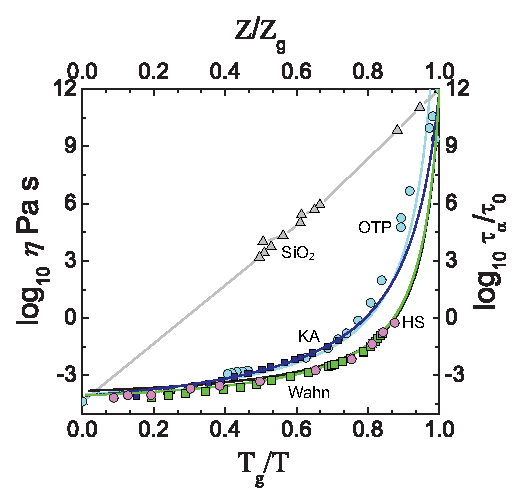
\includegraphics[width=0.9\linewidth,outer]{angell}
  \caption[The Angell plot for model systems undergoing dynamical arrest]{
    The \emph{Angell} plot \cite{AngellJNS1988} for molecular and model glassformers showing the temperature/pressure dependence of viscosity (labelled here as $\eta$) or equivalently relaxation time $\tau_\alpha$.
    The molecular systems \ce{SiO2} and orthoterphenyl (OTP) respectively display the \emph{strong} and \emph{fragile} behaviours described in text, with data obtained from Refs.\ \cite{AngellS1995, BerthierPRE2009}.
    Kob-Anderson (KA) and Wahnstrom (Wahn) are binary mixtures of Lennard-Jones atoms designed to exhibit fragility.
    The compressibility $Z = \beta p / \rho$ is argued to be equivalent to inverse temperature for hard spheres (HS) \cite{BerthierPRE2009}, with data taken from Ref.\ \cite{RoyallJSM2017}.
    Reproduced from Ref.\ \cite{RoyallPR2015}.
  }
  \label{fig:angell}
\end{SCfigure}

Our focus is on soft matter, with hard spheres as the prototypical model, where the  interactions (typically van der Waals attractions) are much weaker than in molecular systems (and absent in hard spheres).
Consequently, there is less of a case for an Arrhenius relationship \eqref{eq:arrhenius-law}, and empirically we find striking deviations from it.
Many systems show \emph{super-Arrhenius} scaling with temperature (Fig.\ \ref{fig:angell}), including mixtures of Lennard-Jones atoms and molecular systems such as orthoterphenyl.
Correspondingly, systems where $\tau_\alpha$ increases more rapidly than exponential are labelled as \emph{fragile}.
A super-Arrhenius scaling of $\tau_\alpha$ implies that the thermodynamic barrier to relaxation $\Delta \Phi_\alpha$ increases with supercooling.
This means that the dynamics fundamentally changes at high densities (or low temperatures), which must be caused by the onset of \emph{collective} (or \emph{cooperative}) effects; given the weakness of bonds in soft matter, we can conclude that many particles must contribute to create a large barrier.
We will discuss this more in the next section.

Some modification is required for hard particle systems, where temperature is not a natural control parameter.
As we argued in the introduction, pressure is the only meaningful state variable.
The authors of Ref.\ \cite{BerthierPRE2009} argue that pressure plays a role equivalent to inverse temperature in athermal systems, because of similarities in their limit behaviour.
Alternatively, we could make a free volume argument, where we expect a relaxation event to involve fluctuations of volume $\Delta V$.
In equilibrium, volume fluctuations are created by reversible work $p \Delta V$ so to leading order%
\marginfootnote{The leading order behaviour can be given more justification by invoking the morphometric approach \eqref{eq:fmt-morphometric-2}, or from more general arguments which we will introduce in section \ref{sec:insertion-as-solvation}.}
we then expect
\begin{equation*}
  \tau_\alpha \sim e^{\beta p \Delta V}.
\end{equation*}
Taking $\Delta V$ as the equivalent of an energy barrier, we find the conjugate variable $\beta p$ does indeed play the role of inverse temperature.
It is usual to work with the dimensionless \emph{compressibility factor}, defined by
\begin{equation}
  Z = \frac{\beta p}{\rho},
\end{equation}
in terms of which hard spheres show the same phenomenology as thermal systems (Fig.\ \ref{fig:angell}); we find that hard spheres are comparable in fragility to various binary Lennard-Jones mixtures.
Relaxation barriers in hard spheres are entropic in nature, so perhaps it is easier to see the need for collective effects.
Moreover, the geometrical interpretation in terms of volume fluctuations $\Delta V$ provides an intuitive picture for collective motion: at high densities more particles have to move out of the way to create space for motion.

\begin{SCfigure}
  \includegraphics[width=0.7\linewidth,outer]{dynamic-heterogeneity}
  \caption[Dynamical heterogeneity in binary hard discs]{
    Dynamical heterogeneity in a binary hard disc system with a size ratio of $1:1.4$.
    Particles are coloured according to distance moved over a relaxation time $\tau_\alpha$, with blue having moved the least and red the most.
    Reproduced from Ref.\ \cite{RoyallPR2015}.
  }
  \label{fig:dynamic-heterogeneities}
\end{SCfigure}

Given the rapid increase in dynamical timescales with supercooling, there comes a point where the relaxation time exceeds the observation time so it is impossible to equilibrate the system.
This is the \emph{experimental glass transition}, operationally set as the point where $\tau_\alpha(T = T_g \textrm{ or } \eta = \eta_g) = \SI{100}{\second}$.
In some sense, this threshold defines a subjective limit of a human observer's patience, and so the point $T_g$ (or $\eta_g$) is not strictly a transition.
However, in practice $\tau_\alpha$ is increasing so rapidly by this point that the location of $T_g$ (or $\eta_g$) is insensitive to the choice of observation time \cite{CavagnaPR2009}.

As the final piece of the phenomenology we introduce two more important dynamical features which differentiates the supercooled liquid from normal liquids.
First, the Stokes-Einstein equation, relating diffusion, temperature and viscosity, holds at high temperatures (low densities) but significant deviations are observed at supercooling to low temperatures (high densities) \cite{BerthierRMP2011}.
This finding possibly suggests the existence of multiple competing relaxation mechanisms in the supercooled liquid, which are probed differently by the two measures \cite{EdigerARPC2000}.
Second, the dynamics becomes highly spatially heterogeneous at increased supercooling (Fig.\ \ref{fig:dynamic-heterogeneities}).
Furthermore, simulation studies have revealed that the initial configuration strongly correlates with the locations of mobile events \cite{Widmer-CooperJPCM2005}.
This suggests that the sites of mobility are encoded in the static configuration, which could be interpreted structurally.
%The size of these hetereogeneities is captured by a dynamic lengthscale $\xi_\mathrm{dyn}$, whereas thermodynamic theories typically concern static lengthscales.
%A requirement of a thermodynamic theory is thus that $\xi_\mathrm{dyn}$ scales with the proposed static length.

%% To unveil static quantities, it is tempting to link dynamical heterogeneity to structural heterogeneity.
%% Stable structures should move less than unstable ones.
%% Widmer-Cooper and Harrowell 11 demonstrated that the initial configuration of a simulation, independently of the initial dynamics, has a role in the heterogeneity of the dynamics.

The main point of contention is over what causes this slow-down: whether it is driven by an underlying phase transition in the thermodynamic viewpoint, or if it is purely a kinetic effect.
The former viewpoint includes the related \emph{mode-coupling} and \emph{random first-order transition} theories, which are loosely based on mean-field theory.
By contrast, the kinetic viewpoint \emph{dynamical facilitation} is based entirely around study of fluctuations.
Having introduced the phenomenology of supercooled liquids we can now proceed to discuss these theories in turn.
We will emphasise the thermodynamic theories because in recent years there has been a substantial shift towards them because of the success of mean-field theories.
Furthermore, our approach focuses on static many-body correlation functions and local structure, which lends itself more towards a thermodynamic viewpoint.

%These are not \emph{completely} mutually exclusive viewpoints, as it is possible hybrid scenarios exist where a phase transition is 

%% We discussed the static correlation functions at length, which is fine for liquids where equilibrium occurs on a \SI{100}{\pico\second} timescale.
%% Dynamical effects are highly nontrivial at high densities.
%% As a practical definition, a glass is defined in the lab as any material for which the relaxation time exceeds \SI{100}{\second}: this point is called the experimental glass transition.
%% This is somewhat arbitrary, although the location of the glass transition point is not particularly sensitive to where you set the threshold because of how rapidly the viscosity/times are increasing around there.
%% So what do we mean by dynamical arrest.

%% Cooling a liquid.
%% Take thermodynamic quantity (e.g.\ volume, entropy, enthalpy): usually crystallise.
%% (Picture)
%% First-order transition bypassed by quick cooling.
%% Enter supercooled liquid phase.

%% Both of these conditions are violated in the glass, as this is a truly non-equilibrium state.
%% That is, we see ageing, and hysteresis in response to perturbations.
%% No longer equilibrates/relax/flows, call it a glass: occurs at glass transition.
%% Glass is a solid for all practical purposes.
%% Distinguished from glass which has dependence on preparation history, hysteresis/memory effect of heating the system (will not follow exactly the same curve until - back to the equilibrium supercooled structure), aging: averages (including correlations) evolve in time.

%% The glass transition itself is not a ``transition'' in the thermodynamic sense; there is no.
%% It's really a kind of impatience transition; the glass transition for a human would be different to the glass transition for a demigod/ent.
%% It's still a relatively robust measurement, because of the superarrhenius scaling (sc-l for pedestrians).

%% A plethora of questions related to the out-of-equilibrium properties.
%% \begin{enumerate}
%% \item Properties of out of equilibrium glass phase: very important questions for material science. Low temperature anomalies, aging behaviour, nonlinear rheology  plasticity.
%% \item Relation between glass and jamming. Jamming=zero temperature, out of equilibrium, infinite pressure.
%% \item How to avoid crystallisation.
%% \end{enumerate}

%% We will talk about this metastable branch as if it were in equilibrium.
%% \todo{create link when mention high density swap data}

%% Relationship with viscosity.
%% Flowing/not flowing is captured by viscosity: viscous slowdown same as relaxation slowdown.
%% Slightly different notion.
%% Short times $t \ll \tau$: elastic system, long times $t \gg \tau$: viscosity.
%% Time barrier is relaxation time.
%% Elasticity, viscosity in Newtonian fluids: viscoelastic behaviour (Maxwell)
%% \begin{equation}
%%   \eta = G_\infty \tau_\mathrm{relax}
%% \end{equation}
%% high frequency shear modulus is elastic property.
%% Shear modulus increases by factor 2-5 times, is dwarfed by change in relaxation time.

\section{Mode-coupling theory}
\label{sec:mct}

The central tenet of mode-coupling theory (MCT) is to separate the liquid's degrees of freedoms into \emph{slow} and \emph{fast} variables.
Fast variables are those that thermalise very quickly, e.g.\ the solvent in a colloidal liquid, so that they can be integrated out leaving only slowly evolving variables of interest.
We advocate essentially the same philosophy, of coarse-graining onto a few dynamically relevant degrees of freedom, in developing a theory for many-body correlations in chapters \ref{chapter:morphometric-framework} and \ref{chapter:morphometric-applications}.
The difference between the two approaches is that MCT explicitly treats \emph{dynamical} processes whereas we focus on \emph{static} correlations.
We will discuss our own approach more in section \ref{sec:correlation-perspective}.

As an example of separation into fast and slow variables, consider classical Langevin equation of motion.
%, which expresses the equations of motion of a subset of the degrees of freedom.
Newton's equation for a particle in an external field becomes
\begin{equation}\label{eq:classical-langevin}
  m \ddot{\vec{r}}
  =
  \vec{\nabla} \phi_\mathrm{ext}(\vec{r})
  - \lambda \dot{\vec{r}} + \vec{f}(t)
\end{equation}
where $m$ is the particle mass, $\lambda$ is a coefficient of damping and $\vec{f}$ is the \emph{fluctuating force} from the fast variables, normally approximated as a Gaussian random field
\begin{equation*}
  \langle f_i(t) f_j(t') \rangle = 2 D \delta_{i,j} \delta(t - t'),
\end{equation*}
with diffusion constant $D$.
Here, the position $\vec{r}$ represents the slowly evolving variable of interest, whereas the remaining degrees of freedom (e.g.\ small solvent particles) are imagined to equilibrate rapidly leaving only the force field $\vec{f}$.

Mode-coupling theory starts from a formally \emph{exact} Langevin equation, which generalises the classical result \eqref{eq:classical-langevin} above.
Defining the instantaneous state of the liquid as
\begin{equation*}
  \vec{X}(t) := \begin{pmatrix} \hat\rho(\vec{r}, t) \\ \vec{\hat{j}}(\vec{r}, t) \end{pmatrix}
\end{equation*}
with instantaneous current $\vec{\hat{j}}(\vec{r}, t) := \partial \hat\rho(\vec{r}, t) / \partial t$, the generalised Langevin equation then reads \cite{ReichmanJSM2005, JanssenFP2018}
\begin{equation}\label{eq:general-langevin}
  \frac{d \vec{\widetilde{X}}(\vec{k}, t)}{dt}
  =
  i \vec{\Omega} \cdot \vec{\widetilde{X}}(\vec{k}, t)
  - \int_0^t \vec{K}(t') \cdot \vec{\widetilde{X}}(\vec{k}, t - t') \, dt'
  + \vec{f}(t)
\end{equation}
where $\vec{f}$ is (again) the fluctuating force obtained by integrating out the fast degrees of freedom, $\vec{K}(t')$ is a time-dependent \emph{memory function} containing the history of $\vec{f}$ as an autocorrelation function \cite{ReichmanJSM2005} and $\vec{\Omega}$ is the \emph{frequency matrix} containing the forces internal to the slow variables \cite{JanssenFP2018}.
Each of these terms has an allegory in the classical Langevin equation \eqref{eq:classical-langevin} above.
Similar equations to \eqref{eq:general-langevin} can be constructed for observables such as the correlation functions; the goal of MCT is to construct (and solve) an equation for $F(\vec{k}, t)$ \eqref{eq:isf} obtaining the dynamical behaviour of the liquid at long times.
The central challenge of this approach is finding suitable approximations for the memory function $\vec{K}$.
%% \begin{equation*}
%%   \vec{K}(t') = \vec{f}(0)^T \vec{f}(t') \cdot (\vec{\widetilde{X}}^T \vec{\widetilde{X}})^{-1}.
%% \end{equation*}

In the standard MCT approach, the fluctuating force is assumed to be dominated by the pair correlations so that $K$ becomes a four-point correlation function.
Then, through a second approximation where $K$ is factorised into a product of two two-point correlation functions, it is possible to construct an evolution equation for the intermediate scattering function \eqref{eq:isf} as \cite{ReichmanJSM2005}
\begin{equation}\label{eq:full-mct}
  \frac{d^2 F(k,t)}{d t^2}
  + \frac{k^2}{\beta m S^{(2)}(k)} F(k, t)
  + \int_0^t K_\mathrm{MCT}(k, t') \frac{d F(k, t - t')}{dt} \, dt'
  =
  0
\end{equation}
with
\begin{subequations}\label{eq:full-mct-coupled}
  \begin{align}
    K_\mathrm{MCT}
    &=
    \frac{\rho}{16 \pi^3 \beta m}
    \int |V_{\vec{q},\vec{k}-\vec{q}}|^2
    F(q, t) F(|\vec{k} - \vec{q}|, t)
    \, d\vec{q},
    \\
    V_{\vec{q},\vec{k}-\vec{q}}
    &=
    \frac{
      \vec{k} \cdot \vec{q} c^{(2)}(q) + \vec{k} \cdot (\vec{k} - \vec{q}) c^{(2)}(|\vec{k} - \vec{q}|)
    }{
      k
    }.
  \end{align}
\end{subequations}
The latter function $V_{\vec{q},\vec{k}-\vec{q}}$ is the so-called \emph{vertex}, which takes the pair direct correlation, and the initial condition for \eqref{eq:full-mct} is $F(k,t=0) = S^{(2)}(k)$; as such, standard MCT takes only pair correlation functions as input.
Together \eqref{eq:full-mct} and \eqref{eq:full-mct-coupled} form a non-linear coupled set of integro-differential equations that can be numerically solved, providing a reasonable description of the \emph{onset} of dynamical arrest, with deviations only becoming noticeable at deep supercooling \cite{FlennerPRE2011,BrambillaPRL2009}.

Crucially, MCT predicts a diverging timescale at $\eta \sim 0.52$ in hard spheres, where the dynamics would become completely arrested, and numerical fits to colloidal experimental data with the same power behaviour law predicted by MCT move this point up to $\eta \sim 0.58$ \cite{VanMegenPRE1994}.
However, this predicted transition must be spurious as recent experiments have managed to equilibrate colloidal hard sphere liquids up to $\eta \lesssim 0.60$ \cite{BrambillaPRL2009,HallettNC2018} and to even higher densities in simulations \cite{BerthierPRL2016}.
Despite this failing of MCT, it remains the only properly first-principles theory for treating liquid dynamics.

Extensions incorporating fluctuations can be found in Refs.\ \cite{BiroliPRL2006,SzamelPTEP2013}, and more recently a generalised MCT has been developed which avoids the uncontrolled factorisation of the pair densities \cite{JanssenPRL2015,JanssenFP2018}.
Importantly, the latter approach incorporates closures of the many-body correlation functions, which will be a central theme of later chapters; by doing this the authors were able to move the diverging timescale to higher densities, bringing the theory into better agreement with available data from simulations and experiments.

\section{Mean-field theories}
\label{sec:mean-field-glass}

We introduced MCT as an explicitly dynamical theory which attempts to model dynamical arrest in supercooled liquids by directly describing the decay of time correlation functions like $F(k, t)$.
Thermodynamics only entered implicitly into MCT through the structural input of the static structure factor $S^{(2)}(k)$.
By contrast, \emph{mean-field theories} of glass take a primarily thermodynamic approach, though they are broadly compatible with the dynamical descriptions of MCT.
The mean-field picture has been rapidly gaining traction in recent years since exact solutions have been developed for hard spheres \cite{ParisiRMP2010,KurchanJSM2012,KurchanJPCB2013,CharbonneauNC2014,CharbonneauJSM2014}.
To describe mean-field theory we will invoke the concept of an \emph{energy landscape}, the natural generalisation of transition state theory introduced in section \ref{sec:glass-phenomenology} and summarised by \eqref{eq:reaction-time}.
While this conceptual framework is not unique to mean-field theories, it is most closely associated with them.

In an energy landscape description, the thermodynamic potential is interpreted \emph{geometrically} as a mapping from every point in configuration space to a `height' representing energy e.g.\ $\Phi: \mathbb{R}^{dN} \mapsto \mathbb{R}$ for an $N$ particle system.
The appeal of this approach is that physical processes can be understood \emph{topographically}: the system will spend more time at the bottom of `valleys' (minima of $\Phi$), especially at lower temperatures, and dynamics will occur primarily through low-lying `mountain passes' (saddles of $\Phi$) \cite{StillingerS1995}.
The timescales of transitions over saddles are expected to scale via the usual Boltzmann weight \eqref{eq:reaction-time}, just as in ordinary transition state theory, however this refined picture emphasises the importance of landscape \emph{connectivity}: the number, separation and relative weights of the various dynamical paths could drive the glass transition.

The energy landscape is particularly relevant in mean-field, formally corresponding to the high dimensional limit%
\marginfootnote{To understand why, consider the typical number of particle neighbours increases with dimensionality.
  Then, formally in the limit $d \to \infty$ a particle is able to achieve a macroscopic number of neighbours, equivalent to an interaction with an average field representing the rest of the system.}
$d \to \infty$, because its \emph{exact} properties can be determined.
In mean-field, hard spheres undergo a \emph{clustering} (or \emph{dynamical}) transition at a volume fraction $\eta_c$ where the landscape splits into disconnected regions \cite{ParisiRMP2010,KurchanJSM2012,KurchanJSM2016}, and the dynamics are described by an almost identical theory to MCT \cite{MaimbourgPRL2016,KurchanJSM2016}.
As configuration space becomes disconnected at $\eta_c$, the system is frozen into a single region and so the relaxation time diverges; contemporaneously, the memory function analogous to $K_\mathrm{MCT}$ in mean-field develops a plateau reflecting the fact that the density profile can no longer completely relax \cite{CharbonneauARCMP2017}.
In this light, the diverging relaxation time predicted by standard MCT is not necessarily a failure of the theory, but is indicative of this genuine mean-field transition.

Although the dynamics is singular at the dynamical transition, the thermodynamic observables are continuous as the system is compressed beyond $\eta_c$ \cite{ParisiRMP2010}.
%% Starting from the definition of the Helmholtz free energy.
%% \begin{equation*}
%%   F = \langle U \rangle - T S.
%% \end{equation*}
We can imagine what happens to the system under further compression if it could continue to sample these disconnected regions in equilibrium, i.e.\ with Boltzmann weighted measure.
The free energy, normally expressed as a sum over all microstates%
\marginfootnote{Which microstates this includes depends on the ensemble.}
$\Gamma$, can be re-expressed as a sum over a collection of \emph{mesostates} $\Gamma = \{\alpha_1, \cdots, \alpha_M\}$ giving
\begin{equation}
%\begin{subequations}
  %\begin{align}
    \Phi = \sum_{i \in \Gamma} p_i \, (\epsilon_i - k_B T \, \ln{p_i})
   % \\
    = \overline{\Phi} - T \Sigma
  %\end{align}
%\end{subequations}
\end{equation}
where $\epsilon_i$ is the energy of microstate $i$ and $p_i$ its probability measure.
In the latter step we defined%
\marginfootnote{This expression is obtained by writing the probability of the system being in mesostate $\alpha$ as $p_\alpha = \sum_{i \in \alpha} p_i$, then $p_i / p_\alpha$ is the probability of microstate $i$ given that the system is in this mesostate.}
\begin{subequations}
  \begin{align}
    \overline{\Phi}
    &=
    \sum_\alpha p_\alpha
    \underbrace{
      \sum_{i \in \alpha} \frac{p_i}{p_\alpha}
      \left(
      \epsilon_i - k_B T \, \ln{\frac{p_i}{p_\alpha}}
      \right)
    }_\textrm{free energy of mesostate $\alpha$},
    \\
    \Sigma &= - k_B \, \sum_\alpha p_\alpha \ln{p_\alpha}.
  \end{align}
\end{subequations}
The \emph{complexity} $\Sigma$ is an extensive quantity characterising the multiplicity of mesostates; at the dynamical transition this becomes a positive non-zero number $\Sigma(\eta = \eta_c) > 0$ corresponding to the clustering in configuration space.
As the system is compressed further $\Sigma$ decreases \cite{KirkpatrickPRB1987,KirkpatrickPRA1989,ParisiRMP2010} corresponding to the rarefaction of clustered regions.
At a volume fraction $\eta_K > \eta_c$ an \emph{entropy crisis} occurs: $\Sigma$ vanishes, leading to the system being frozen into a single, unique region in configuration space called an \emph{ideal glass} phase \cite{KauzmannCR1948,KirkpatrickPRB1987,HallJCP1987,KirkpatrickPRA1989,ParisiRMP2010,BerthierRMP2011}.

If an equilibrium glass state in the regime $\eta \in [\eta_c, \eta_K]$ is compressed out-of-equilibrium without sampling the other clusters, a further phase transition occurs to a so-called \emph{Gardner} phase \cite{KurchanJPCB2013,CharbonneauNC2014,CharbonneauJSM2014}.
Each cluster splits further into fractal sub-regions arranged hierarchically.
Whereas the clustered regions formed at $\eta_c$ are geometrically dissimilar%
\marginfootnote{As measured by e.g.\ the intermediate scattering function},
these regions are close in configuration space to one another.
This phase has deep connections with the jamming transition seen at diverging pressure, providing a unified description of glass and jamming conjectured since the landmark paper of Ref.\ \cite{LiuN1998}.
Remarkably, this mean-field theory is able to predict anomalous $d$-independent critical scaling coefficients, matching those known around jamming \cite{WyartPRL2012,LernerSM2013,DeGiuliPNAS2014}.
The existence of the Gardner phase provides context for the importance of mean-field theory, but it cannot be directly connected to our approach in subsequent chapters so we will not discuss it further.
For more information on the mean-field Gardner phase see the reviews of Refs. \cite{BerthierJCP2019,CharbonneauARCMP2017}.

%% Specifically, the glass transition can be understood as the division of the energy landscape up into subunits??
%% Exact properties of the energy landscape can be determined for many mean-field systems, where it is known to play a leading role in dynamical arrest.

The mean-field picture introduces complexity as the important quantity of interest, relating the number of metastable regions in configuration space.
The relevance of mean-field descriptions in physical dimensions requires a finite-dimensional description of the supercooled liquid and its energy landscape.

%% In physical dimensions, the energy landscape does not become completely disconnected, so transitions between metastable states are possible; the dynamical transition becomes a cross-over.
%% As such, a finite-dimensional description of the supercooled liquid is needed.

%% In physical dimensions, the energy landscape does not become
%% This quantity is well-defined in mean-field because these regions are completely disconnected, however in finite dimensions transitions can always occur between them through nucleation \cite{KirkpatrickPRB1987,KirkpatrickPRA1989,BouchaudJCP2004}.
%% The dynamical transition thus becomes a cross-over, and a finite-dimensional description of the supercooled liquid is needed.

\section{Finite-dimensional theories}
\label{sec:finite-d-glass}

\begin{SCfigure}
  \includegraphics[width=0.9\linewidth,outer]{swap-Sconf}
  \caption[Configurational entropy in hard spheres from Monte-Carlo simulations]{
    Configurational entropy in hard spheres from novel Monte-Carlo (MC) simulations for a system with 23\% polydispersity.
    $Z_0 \approx 18$ ($\eta_0 \approx 0.56$) marks the onset pressure, above which the intermediate scattering function $F(k,t)$ decays non-exponentially, and $Z_c \approx 23.5$ ($\eta_c \approx 0.598$) is the location of the dynamical transition predicted by fitting mode-coupling theory's power-law scaling to the lower density behaviour.
    The various methods used (described in Ref.\ \cite{BerthierPNAS2017}) all broadly agree that this quantity is trending to zero at a finite pressure, suggesting the existence of a thermodynamic glass transition.
    The equation of state for this system is given in Fig.\ \ref{fig:swap-eos}.
    Reproduced from Ref.\ \cite{BerthierPNAS2017}.
  }
  \label{fig:swap-sconf}
\end{SCfigure}

%% Mean-field theories have traditionally been formulated in configuration space, in terms of the energy landscape.
%% By contast, in $d=3$ the existence of dynamical heterogeneity calls for a real space interpretation.

The relevance of mean-field ideas in physical dimensions can be seen by an interpretation of Refs.\ \cite{KirkpatrickPRB1987,HallJCP1987,KirkpatrickPRA1989}, with antecedent ideas found in \cite{KauzmannCR1948,AdamJCP1965}.
This \emph{random first-order transition} (RFOT) scenario acknowledges that the clustering of states appearing at the dynamical transition in mean-field will not be strictly metastable over finite lengthscales in finite $d$ \cite{BouchaudJCP2004,MontanariJSP2006}.
As such, the complexity is not well-defined because the metastable states will not be strictly separated with infinite barriers, though they may be arbitrarily long-lived; the dynamical transition of mean-field thus becomes a cross-over.
In finite dimensions, the \emph{configurational entropy} $S_\mathrm{conf}$ is introduced as the closest equivalent to the complexity; this does not have a generally agreed upon meaning, but a common definition invokes the timescale separation between vibrational ($\beta$--) and liquid-like ($\alpha$--) dynamics.
The configurational entropy then describes the entropy of the latter process, obtained as the residual entropy after removing vibrations
\begin{equation}\label{eq:sconf}
  S_\mathrm{conf} := S - S_\mathrm{vib},
\end{equation}
though some refinement is required for polydisperse systems \cite{OzawaJCP2017,OzawaJCP2018} and where additional non-vibrational processes exist that do not relax the density profile \cite{OzawaPRL2018}.

The RFOT scenario imagines the mean-field dynamical transition as a crossover to an \emph{energy landscape dominated} dynamics.
Specifically, the number of unique (non-vibrational) states possible in a subregion of size $\xi$ will scale $\propto \exp{(s_\mathrm{conf} \xi^d / k_B)}$, where $s_\mathrm{conf} = S_\mathrm{conf} / V$ is the configurational entropy density.
A dynamical event which changes a state is expected to pay an energy penalty $\gamma_\mathrm{eff} \xi^\theta$ where $\theta \le d$ from inducing a mismatch with the surrounding fluid.
The thermodynamic potential for this subregion is then expected to adopt the form
\begin{equation}\label{eq:rfot-barrier}
  \Phi \sim \gamma_\mathrm{eff} \xi^\theta - T s_\mathrm{conf} \, \xi^d.
\end{equation}
The maximum of $\Phi$ occurs at the \emph{point-to-set}%
\marginfootnote{So-named because this lengthscale marks the crossover from the subregion being confined to a single `point' in its configuration space to a `set' of states.}
length
\begin{equation}\label{eq:rfot-xi}
  \xi_\mathrm{PS}
  := \argmax{(\Phi)}
  \sim
  \left(
  \frac{\theta \gamma_\mathrm{eff}}{d T s_\mathrm{conf}}
  \right)^\frac{1}{d-\theta},
\end{equation}
after which $\Phi$ grows infinitely negative, so the metastable states are unstable to activated dynamics for $\xi \gtrsim \xi_\mathrm{PS}$.
The RFOT interpretation thus predicts the formation of a \emph{mosaic} of droplets of typical lengthscale $\xi_\mathrm{PS}$ \cite{KirkpatrickPRB1987,HallJCP1987,KirkpatrickPRA1989,BouchaudJCP2004}.
The nature of the entropic droplets forming the mosaic state and the processes by which they relax is an active area of study \cite{BouchaudJCP2004,DzeroPRB2005,FranzJSM2005,AngeliniJSP2017,RulquinJSM2016,BiroliMeanPRB2018,BiroliFinitePRB2018}.
Notably, a lot of attention has been devoted to the treatment of the subleading term $\gamma_\mathrm{eff} \xi^\theta$.

This thermodynamic argument above concerns whether a region of the liquid \emph{will} relax eventually, but an even more direct connection with relaxation timescale was proven in Ref.\ \cite{MontanariJSP2006}.
Briefly, dynamical barriers must remain finite within a finite subregion, so they scale Arrheniusly via \eqref{eq:reaction-time}; any Arrhenius process will eventually overwhelm the super-Arrhenius scaling of $\tau_\alpha$ at deep supercooling.
Fragile behaviour then suggests a reduction in $S_\mathrm{conf}$ to limit the number of possible Arrhenius processes.
Moreover, the authors of Ref.\ \cite{MontanariJSP2006} then show that the relaxation time is rigorously bounded from above by $S_\mathrm{conf}$, proving that any diverging relaxation time \emph{must} coincide with an entropy crisis where $S_\mathrm{conf}$ becomes sub-extensive.
Measurements of the configurational entropy from simulations of hard spheres suggest a vanishing $S_\mathrm{conf}$ at finite pressure in $d=3$ (Fig.\ \ref{fig:swap-sconf}), pointing to a mean-field/RFOT scenario in hard spheres.
However, this necessarily relies on extrapolation as the point where $S_\mathrm{conf}$ vanishes cannot be reached in finite time because of the argument above.

%% Mean-field argument is thermodynamic, which in some sense is structural.
%% Structural in the sense of the energy landscape, not necessarily in real space/local structure.
%% The real space interpretation of mean-field theory is random first-order transition theory (RFOT), also called \emph{mosaic} theory.

%% In conventional condensed matter physics dynamics is determined by structure.
%% For example, crystalline solids are fixed on a lattice so do not flow, whereas liquids are disordered and are thus able to flow.
%% Soft matter systems (e.g.\ gels, foams, glasses) do not neatly fall into this paradigm: their dynamics are often arrested whilst their structure remains highly disordered.

\begin{SCfigure}
  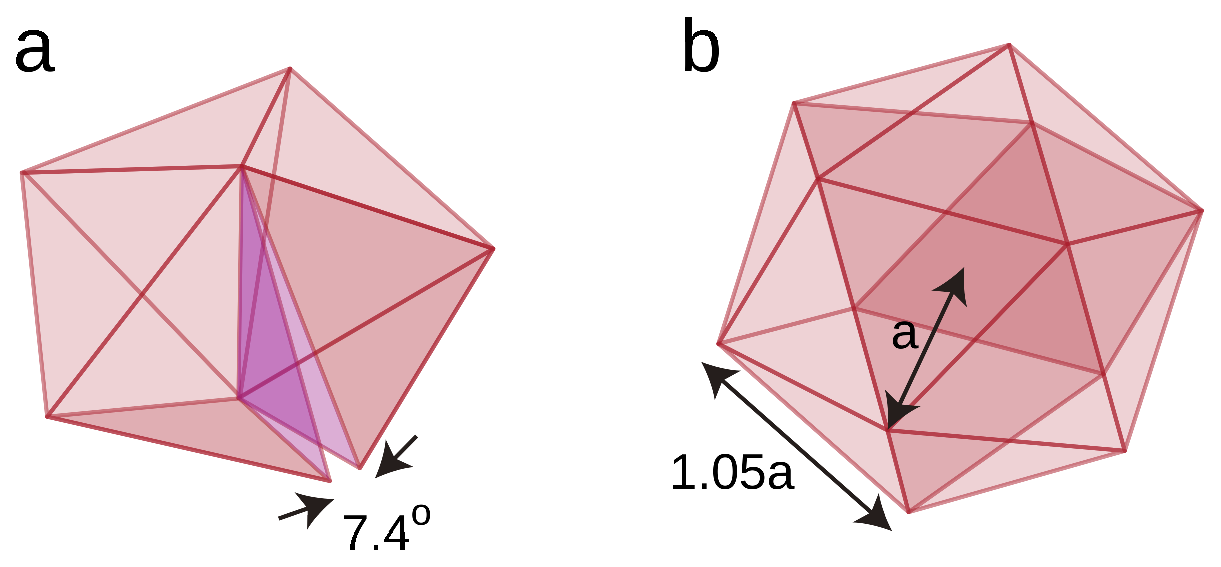
\includegraphics[width=0.7\linewidth,outer]{frustration}
  \caption[Frustration of tetrahedral structures]{
    Structures formed by combining tetrahedra.
    (a) The pentagonal bipyramid constructed from five regular tetrahedra must leave a small gap of \SI{7.4}{\degree}.
    (b) The icosahedron formed by vertices a distance $a$ from the centroid must have edge length $\sim1.05 a$, so if hard spheres of diameter $a$ were placed on the vertices they would not be in contact.
    Reproduced from Ref.\ \cite{RoyallPR2015}.
  }
  \label{fig:frustration}
\end{SCfigure}

A different scenario in physical dimensions focuses on the role of geometry.
This picture starts from the observation that crystal structures (e.g.\ the face-centred cubic introduced for hard spheres at close packing) are generally not the optimal energetic arrangement for small clusters of particles, even though they must be for bulk systems.
For example, 13 isolated Lennard-Jones atoms will preferentially arrange as vertices of a fivefold symmetric \emph{icosahedron} \cite{FrankPRS1952} (Fig.\ \ref{fig:frustration}b).
As fivefold symmetric structures cannot tessellate Euclidean space, Sir Charles Frank conjectured that glassformers suppress crystallisation through formation of icosahedra (or similar structures) \cite{FrankPRS1952}.

The above viewpoint has been developed into the more complete theory called \emph{geometric frustration} \cite{KivelsonPA1995,TarjusJPCM2005}.
This approach characterises the liquid by its \emph{locally favoured structures} (LFS), i.e.\ those structures which are energetically favoured at small length scales.
A system could have a single LFS, or a whole collection; recently, it has been shown through numerical simulations that \emph{competition} between different LFS enhances the propensity for glassformation \cite{TeichNC2019}.
This competition is an example of \emph{frustration} where continual growth of domains of LFS is hindered by geometric constraints.
Frustration can also emerge from a single LFS if it cannot tile space, as is the case of fivefold symmetric structures like icosahedra.
Incorporating frustration into a theory modelling the energy of LFS-rich domains leads to a similar scaling relation as in RFOT \eqref{eq:rfot-barrier}, though the resulting phase behaviour is quite different.
The static lengthscale which emerges from this theory is interpreted as the size of the domains, which is more easily understood than the amorphous lengthscale $\xi_\mathrm{PS}$ of RFOT.
Details can be found in the review of Ref.\ \cite{TarjusJPCM2005}.

The frustration picture is broadly compatible with the mean-field viewpoint: the propensity for a system to form certain structures can be interpreted as a manifestation (or a driving force) of a reduced $S_\mathrm{conf}$.
The downside of this scenario is that the correlation between local structure and dynamics seems to be highly system dependent \cite{HockyPRL2014}.

Whereas RFOT postulates amorphous order, geometric ideas propose simpler static orderings based around e.g.\ LFS domains.

CPR: local structure fixes gel \cite{RoyallNM2008}.
Charbonneau: growth of length scale associated with LFS does not correlate with dynamical length scale \cite{CharbonneauPRL2012}, possibly multiple relaxation mechanisms or a non-static length scale.
Leacmach: \cite{LeocmachNC2012}
Coslovich: \cite{CoslovichJCP2007,CoslovichJCP2007a}
Turci: \cite{TurciPRL2017}

In hard spheres, the dominant LFS are found to be icosahedral motifs in accordance with Frank's original conjecture.
In Fig.\ \ref{fig:icosahedral-domains} we see the growth of large domains of icosahedra in the supercooled liquid, over a range in densities where $\tau_\alpha$ changes by a factor of $\mathcal{O}(10^5)$ (Fig.\ \ref{fig:g2-changes}) \cite{HallettNC2018}.
This fact demonstrates that significant structural change occurs alongside dynamical arrest, even though minimal changes are seen at the pair level.
This does not prove that structural change \emph{causes} the slowdown, but it does suggest the idea is worth investigating.
%Furthermore, the vicinity of an icosahedral motif is found to be highly correlated with local particle mobility \cite{HallettNC2018}.

%At high densities the tetrahedra form large connected domains \cite{HallettNC2018} rich in fivefold symmetric structures.
Spherical packings ideally form regular tetrahedra which cannot perfectly form pentagonal structures (Fig.\ \ref{fig:frustration}), so fivefold symmetric structures are highly frustrated.
A detailed review on the role of local structure in glassy systems can be found in Ref.\ \cite{RoyallPR2015}.
\todo{Should definitely cite more Royall group work here, possibly Tanaka too. What's the most appropriate cross-section of papers?}

%% The mean-field picture of glass formation interprets the dynamical slowdown entirely within a thermodynamic framework.
%% In mean-field hard spheres, formally in the limit of infinite spatial dimensions $d \to \infty$,
%% Hard spheres in mean field have been shown to have a thermodynamic glass transition, however the critical dimensions are unknown so it is unclear what happens in $d=3$. \cite{ParisiRMP2010,KurchanJSM2012,KurchanJPCB2013,CharbonneauNC2014,CharbonneauJSM2014}.
Recent numerical evidence suggests that $S_\mathrm{conf}$ only vanishes at $T=\SI{0}{\kelvin}$ for a model glassformer in $d=2$ \cite{BerthierNC2019}.
As this point cannot be crossed no thermodynamic transition can occur in $d = 2$, pointing to a lower critical dimension for mean-field theory of at least $d_L \ge 2$.
It is possible that low-dimensional fluctuations prevent any thermodynamic transition, and it has been argued that even if there is a thermodynamic transition at $\eta_K$ this may not be responsible for the dynamic slowdown seen around the operational glass transition $\eta_g \ll \eta_K$ \cite{WyartPRL2017}.
As such, there is room for alternative pictures to the mean-field/RFOT scenario.

The main opposition theory is \emph{dynamic facilitation}, which focuses on the dynamic heterogeneities as the fundamental feature of glass.
In this picture dynamical events occur through string-like motion between dynamical defects, and the relaxation time remains finite until $T = \SI{0}{\kelvin}$.
\todo{Paddy: Expand on this substantially}
For more information on dynamic facilitation we direct the reader to the review of Ref.\ \cite{ChandlerARPC2010}.
%This must trivially occur at the very least $T=0\si{K}$ where relaxation timescales diverges, however much like the lack of a phase transition in the Ising model in $d=1$ this is not a true thermodynamic phase transition because it cannot be crossed.
%So the central question of glass is what happens in $d=3$, is there a vanishing configurational entropy at a finite $T > 0$ with an accompanying thermodynamic glass transition?

%Theories concentrating on the high density glass: elastic theories.

\begin{SCfigure}
  \includegraphics[width=\linewidth,outer]{icosahedra-hallett}
  \caption[Growth of icosahedral domains in the supercooled hard sphere liquid]{
    Growth of icosahedral domains in a colloidal hard sphere liquid with supercooling, i.e.\ increased volume fraction $\eta$, over a density change which coincides with minimal structural change at the pair level (Fig.\ \ref{fig:g2-changes}).
    (a) STED nanoscopy image for $\eta = 0.598$, with scale bar \SI{3}{\micro\meter}.
    (b), (c) Rendered coordinates of partial icosahedra (green, top right structure) and full icosahedra (purple, bottom right structure) for volume fractions (b) $\eta = 0.523$ and (c) $\eta = 0.598$.
    Reproduced from Ref.\ \cite{HallettNC2018}.
  }
  \label{fig:icosahedral-domains}
\end{SCfigure}

\section{Perspective: usefulness of many-body correlations}
\label{sec:correlation-perspective}

In subsequent chapters will be heavily focusing on the treatment of static many-body correlation functions in the bulk liquid.
Here, we motivate their study for the treatment of the supercooled liquid.
It is natural to wonder what new information can be obtained from the many-body correlation functions that is not already present at the pair level.
In section \ref{sec:thermodynamic-routes} we saw how the compressibility and virial routes lead to expressions of the free energy in terms of pair correlations.
This is emblematic of conventional routes to the free energy, so in some sense all of the thermodynamically relevant information is contained in the two body correlation functions.

Firstly, while it is true that thermodynamic quantities like the pressure can certainly be inferred from the pair correlations, there is no such simple relationship for dynamical quantities.
In the absence of a thermodynamic phase transition, we would not expect the pair correlation function alone to reveal much about the nature of dynamical arrest, beyond the lack of a transition.
Even supposing the existence of a transition, the precision required to detect such a signal $g^{(2)}(r)$ may be arbitrarily subtle; however, any changes approaching a transition \emph{must} be magnified at the many-body level because of \eqref{eq:correlation-derivatives}.
The many-body correlation functions have potential to place the entropic droplet scenario of \eqref{eq:rfot-barrier} on more rigorous footing, by providing a means to calculate the subleading penalty term $\gamma_\mathrm{eff} \xi^\theta$.
Alternatively, the theories which postulate local mechanisms such as the LFS in geometrical viewpoints or the dynamical defects in facilitation should be identifiable within the many-body correlation functions.

Secondly, even at the thermodynamic level the many-body correlations have advantages.
To illustrate this we borrow an argument originally made by Evans \cite{EvansPrivate2019}.
Pair correlations yield thermodynamic quantities which are \emph{derivatives} of the free energy at an instantaneous state point, so to infer the free energy multiple state points must be sampled.
Equivalently, we could consider the derivatives of the pair correlation function.
It is straightforward to show that \cite{Santos2016}
\begin{equation}\label{eq:correlation-derivatives}
  \chi_T \rho
  \left( \frac{\partial \rho^{(n)}}{\partial \rho} \right)_{V,T}
  =
  (n - \rho V) \rho^{(n)}(\vec{r}^n)
  + \int \rho^{(n+1)}(\vec{r}^{n+1}) \, d\vec{r}_{n+1}.
\end{equation}
The important feature to take away from this expression is the presence of $\rho^{(n+1)}$; we see the emergence of higher-order correlation functions in the derivatives.
This means we could in principle measure the free energy at a single state point by introducing highly accurate measurements of the many-body correlation functions.
This is essentially the spirit of the \emph{entropy route}, which writes \cite{WallaceJCP1987}
\begin{equation}
  S = \sum_{n=1}^\infty S_n
\end{equation}
with entropic terms $S_n$ containing contributions from $n$-particle correlations.
The first few terms are given by \cite{WallaceJCP1987}
\begin{subequations}
  \begin{align}
    \frac{S_1}{V}%\langle N \rangle}
    &=
    k_B \, \rho \left( \frac{d}{2} - \ln{\rho \Lambda^d} \right),
    \\
    \frac{S_2}{V}%\langle N \rangle}
    &=
    \frac{\rho^2}{2 T}
    \int g^{(2)}(\vec{r}) \ln{g^{(2)}(\vec{r})}
    \, d\vec{r},
    \\
    \frac{S_3}{V}%\langle N \rangle}
    &=
    \frac{\rho^3}{6 T}
    %\int g^{(3)}(\vec{r}, \vec{r}') \delta w^{(3)}(\vec{r}, \vec{r}')
    \int g^{(3)}(\vec{r}, \vec{r}')
    \ln{\left(
      \frac{
        g^{(3)}(\vec{r}, \vec{r}')
      }{
        g^{(2)}(\vec{r}) g^{(2)}(\vec{r}') g^{(2)}(\vec{r} - \vec{r}')
      }
      \right)}
    \, d\vec{r} d\vec{r}'.
  \end{align}
\end{subequations}
Then, for a pair-interacting system the excess free energy is obtained as
\begin{equation*}
  \begin{split}
    \frac{\beta F^\mathrm{ex}}{V}
    =& \; \hphantom{ + } \;\,
    \frac{\rho^2}{2} \int g^{(2)}(\vec{r})
    \left( \beta u(\vec{r}) - \ln{g^{(2)}(\vec{r})} \right)
    d\vec{r}
    \\ & \;
    + \frac{\rho^3}{6}
    %\int g^{(3)}(\vec{r}, \vec{r}') \delta w^{(3)}(\vec{r}, \vec{r}')
    \int g^{(3)}(\vec{r}, \vec{r}')
    \ln{\left(
      \frac{
        g^{(3)}(\vec{r}, \vec{r}')
      }{
        g^{(2)}(\vec{r}) g^{(2)}(\vec{r}') g^{(2)}(\vec{r} - \vec{r}')
      }
      \right)}
    \, d\vec{r} d\vec{r}'
    \\ & \;
    + \mathcal{O}\left( \rho^4 g^{(4)}(\vec{r}, \vec{r}', \vec{r}'') \right),
  \end{split}
\end{equation*}
so the free energy can be directly obtained from accurate determination of the correlation functions.
%Similarly, a theory treating the many-body correlation functions must have the free energy (and phase behaviour) built in.

We will be focusing on many-body correlations in real space, to explore the local mechanisms proposed in theories of the glass transition described above.
In some situations the correlations in Fourier space may be more useful, most notably in MCT where many-body generalisations have already found some traction \cite{JanssenPRL2015,JanssenFP2018}.
In principle, our real space correlation functions can be Fourier transformed to obtain these, but in practice this is prohibitively expensive because of the high dimensionality of the arguments for even modest values of $n$.
However, FMT already provides an easy route to obtaining all the correlation functions in Fourier space, as described by the original papers \cite{RosenfeldPRL1989,RosenfeldJCP1990}.
We show how to obtain these below.

Fourier transforming the direct correlation functions for the uniform liquid \eqref{eq:fmt-direct-correlations-uniform-density}, and applying the convolution theorem, allows us to write the rather succinct
\begin{equation}
  \widetilde{c}^{(n)}(\vec{k}^n)
  =
  - \sum_{\alpha_1, \alpha_2, \cdots, \alpha_n}
  \partial^n_{\alpha_1, \alpha_2, \cdots, \alpha_n} \beta f^\mathrm{ex} \;
  \left( \prod_{i=1}^n \widetilde{\omega}_{\alpha_i}(\vec{k}_i) \right)
  \delta(\vec{k}_1 + \vec{k}_2 + \cdots + \vec{k}_n).
\end{equation}
The delta function enforces the `ring' condition $\sum_{i=1}^n \vec{k}_i = 0$ which emerges from translational symmetry of the weight functions, reducing the dimensionality of the domain by $d$.
A further $d(d-1)/2$ degrees of freedom%
\marginfootnote{This many degrees of freedom can be removed for general $n \ge d$, but we expect fewer for $n < d$.
  For example, $n=2$ arrangements (a dimer) are isomorphic to a line so they possess $d-1$ rotational degrees of freedom.}
can be removed by exploiting rotational symmetry.
Many-particle generalisations of the static structure factor can be obtained from $\widetilde{c}^{(n)}(\vec{k}^n)$ by functionally differentiating the Ornstein-Zernike equation \eqref{eq:ornstein-zernike-generic} with respect to density \cite{BarratMP1988}.

\section{Summary}

This concludes the relevant background in supercooled liquids and glasses.
In subsequent chapters we will develop a framework for treating the many-body correlation functions in real space, with the hope that it can address some of the questions outlined here.
\todo{More more more, according to Paddy. ``What does it all mean?'' Static lengthscales $=n$}

\ifdefined\includebibliography
  \newgeometry{margin=1in}
  \printbibliography
\fi

\end{document}

\end{document}

\documentclass[12pt]{report}
\usepackage{preamble}
\setcounter{chapter}{2}

\begin{document}
\chapter{Morphological framework for many-body correlations}
Mostly theoretical but with some numerical experiments which motivate/justify developments to the theory.
The main body of numerical work is left to the following chapter.

\section{Formalism for many-body correlations}
A generalised potential distribution theorem and the potential of mean force.

\section{Morphological form of the potential of mean force}
Justification of assumptions: additivity, continuity and motion invariance
\subsection{Limitations known from DFT literature}
\subsection{As a generalisation of scaled particle theory}
And the limitations this implies.

\section{Worked examples where morphometric form can be exact}
Under certain conditions.
\subsection{Low density limit in arbitrary dimensions from lowest order terms in the virial expansion of the pressure}
\subsection{Arbitrary densities at large lengthscales}
\subsection{Hard rods (dimension d = 1) at all densities}
\subsubsection{Exact result from DFT}
\subsubsection{Morphometric result}
Explore where additivity, continuity and motion invariance apply.
\subsubsection{Implications for higher dimensions}

\section{Derivation of thermodynamic coefficients for hard spheres in $d = 3$}

\section{Accuracy of predicted distribution functions in $d = 3$}
\subsection{Comparison with molecular dynamics simulations}
\subsection{Comparison with Kirkwood superposition approximation}

\end{document}

%TC: macro \marginfootnote [other]
%TC: envir SCfigure [] other
%TC: macrocount beginSCfigure [figure]
\documentclass[11pt,twoside]{report}
\usepackage{preamble}
\setcounter{chapter}{3}
\graphicspath{{../img/}}
\def\includebibliography{}

\externaldocument{background}
\externaldocument{morphometric-framework}

\begin{document}
\chapter{Local structure in the hard sphere liquid}
\epigraph{\textbf{hardball 1.1} \emph{informal} Uncompromising and ruthless methods or dealings.}{Oxford English Dictionary}
\label{chapter:morphometric-applications}
\todo{Check which version of dictionary.}

The majority of this chapter contains work published as Ref.\ \cite{RobinsonPRL2019}.
Later stuff is new.

\section{Introduction}

While mean-field theories provide insight into complex phenomena, physical accuracy is ensured only by a proper treatment of correlations.
For example, the simplest case of two-body correlations is at the foundation of predictive theories of the liquid state \cite{Hansen2013}, colloids, and complex plasmas \cite{LikosPR2001,Ivlev2012}.
%, and some forms of active matter \cite{Bechinger2016}.
In particular, the thermodynamics of simple liquids with solely pairwise interactions can be exactly expressed in terms of two-body correlations \cite{Hansen2013}.
However, to resolve these integrated quantities \emph{spatially} into structural motifs, and \emph{temporally} into specific dynamical events, one needs to calculate many-body correlations.
While such a many-body approach may often be neglected in normal liquids, long-standing challenges such as the dramatic dynamical changes occurring in supercooled liquids approaching their glass transition \cite{BerthierRMP2011,RoyallPR2015} and phase transitions such as crystal nucleation \cite{RussoSR2012} call for a many-body description.

In the case of supercooled liquids, theories based on pair correlations such as the standard mode-coupling framework \cite{goetze} fail to account for activated events thus predicting a spurious ergodicity breaking transition \cite{BrambillaPRL2009,HallettNC2018}.
Activated dynamics are often rationalised through collective (i.e.\ many-body) effects within contrasting thermodynamic and purely dynamic scenarios \cite{LubchenkoARPC2007,TarjusJPCM2005,BiroliPRL2006,JanssenPRL2015,SzamelPTEP2013,ChandlerARPC2010}.
These include exact mean-field results in high dimensions \cite{ParisiRMP2010,CharbonneauARCMP2017} whose relevance in finite-dimensional systems is hotly debated \cite{WyartPRL2017}.
A finite-dimensional theoretical description of many-body effects is therefore much needed.

However, many-body correlations are challenging to compute and typically combine both energetic and entropic contributions.
Physical insight can be gleaned by exploring the potential energy landscape of isolated clusters \cite{Wales2004,ArkusPRL2009}, but such methods are only exhaustive for small system sizes.
This limitation has been partly addressed by embedding clusters in a mean-field approximation of the surrounding liquid \cite{MossaJCP2003,MossaJNS2006}.
\todo{Describe Mossa and Tarjus approach in detail.}
Nonetheless, this approach neglects by construction the intra-cluster entropic contributions that may dominate in the supercooled regime of interest.
Furthermore, computer simulations, which naturally deliver full many-body correlations are limited in the range of dynamics they can access, hampering an approach to the glass transition, except for recent developments for certain models \cite{BerthierPRL2016}.

Here we place theoretical predictions of many-body local structure on a fundamentally more rigorous footing using inhomogeneous liquid state theory \cite{EvansAP1979}, which we reviewed in section \ref{sec:dft} and advanced in the chapter \ref{chapter:morphometric-framework}.
We model the many-body interactions between a local subsystem and the remaining liquid, directly accessing the many-body \textit{free} energy of local arrangements of particles.
This allows us to predict the populations of specific local structures in the bulk system across the entire liquid phase and beyond the dynamically accessible supercooled regime.
\todo{Make clear that in terms of glassy theories our approach does lean more towards a local structure point of view.}

\section{Many-body correlations and surface tension}

We conceptually separate the liquid into $n$ spatially adjacent particles and the remaining degrees of freedom, acting as a solvent, which we treat within the grand-canonical ensemble, as sketched in Fig.\ \ref{fig:system}(a).
The joint probability density for simultaneously finding $n$ identical particles embedded in $\mathbb{R}^d$ at positions $\vec{r}^n := \{\vec{r}_1, \dots, \vec{r}_n\}$ \todo{Move this definition to an earlier chapter} is proportional to the \emph{$n$-particle distribution function} $g^{(n)}(\vec{r}^n)$ \cite{Hansen2013}.
For a homogeneous system, this can be formally expressed in terms of the \emph{potential of mean force}, the reversible work required to insert the particles at $\vec{r}^n$:
\begin{equation}\label{eq:potential-mean-force}
  \begin{split}
    \phi^{(n)}(\vec{r}^n) &\equiv - k_B T \ln g^{(n)}(\vec{r}^n) \\
    &= U(\vec{r}^n) + \Delta \Omega(\vec{r}^n) - n\mu^{ex}.
  \end{split}
\end{equation}
We denote by $U$ the total potential energy of the $n$ interacting particles and by $\Delta\Omega := \Omega - \Omega_\textrm{hom}$ the difference between the grand potential of the homogeneous liquid $\Omega_\textrm{hom}$ (related to the total volume and pressure by the relation $\Omega_\textrm{hom} = -pV$) and the grand potential of the system including the $n$-particle inhomogeneity.
Finally, $k_B T$ and $\mu^{ex}$ are the thermal energy and the excess chemical potential (with respect to the ideal gas) of the homogeneous liquid respectively.

For systems with excluded volume interactions, we can divide the space into a local component $\mathcal{L} \subset \mathbb{R}^d$ of volume $V_\mathcal{L}$ inaccessible to solvent degrees of freedom and the remaining space $\mathcal{R} = \mathbb{R}^d \setminus \mathcal{L}$ filled by solvent (Fig. \ref{fig:system}).
The dividing surface $\partial\mathcal{L}$ separates these two components with surface area $A_{\partial\mathcal{L}}$, creating a surface tension $\gamma$.
The solvent contribution to Eq.\ \eqref{eq:potential-mean-force} is then \begin{equation}\label{eq:surface-tension}
  \Delta \Omega[\mathcal{L}] =
  p V_\mathcal{L} + \gamma[{\partial\mathcal{L}}] A_{\partial\mathcal{L}}.
\end{equation}
Note that the surface tension is not unique as only the total grand potential must be independent of the choice of $\partial\mathcal{L}$ and can even change its sign for some choices of dividing surface \cite{BrykPRE2003}.
For simplicity we will consider one-component liquids with particles of diameter $\sigma$.
Letting $B_R(\vec{r}_i)$ denote a ball of radius $R$ at site $\vec{r}_i$, we choose the \emph{solvent accessible surface} \cite{LeeJMB1971} as the dividing surface such that $\mathcal{L} = \cup_{i=1}^n B_\sigma(\vec{r}_i)$ (Fig.\ \ref{fig:system}).

Following Ref.\ \cite{KonigPRL2004} we assume $\Delta\Omega$ is translation and rotation invariant, continuous (with respect to the Hausdorff metric), and additive.
Hadwiger's characterisation theorem \cite{Hadwiger1957} then ensures the surface tension adopts the so-called \emph{morphometric} form
\begin{equation}\label{eq:morphometric-surface-tension}
  \gamma[\partial\mathcal{L}] =
  \gamma_\infty +
  \frac{\kappa \, C_{\partial\mathcal{L}} + \overline{\kappa} \, X_{\partial\mathcal{L}}}
       {A_{\partial\mathcal{L}}},
\end{equation}
with integrated mean and Gaussian curvatures $C_{\partial\mathcal{L}}$ and $X_{\partial\mathcal{L}}$, and $\gamma_\infty,\kappa,\overline{\kappa}$ as thermodynamic coefficients to be determined.
$\gamma_\infty$ is the surface tension at a planar wall (i.e.\ the familiar macroscopic surface tension), whilst $\kappa$ and $\overline{\kappa}$ are ``bending energies'' accounting for curvature corrections occurring at small length scales.
These values are system (and state point) dependent, but do not depend on the local geometry, making the linear form of Eq.\ \eqref{eq:morphometric-surface-tension} desirable for calculation.
While strictly an approximation, we motivate Eq.\ \eqref{eq:morphometric-surface-tension} from numerical studies where it has been found to be highly accurate below the freezing volume fraction in hard spheres \cite{RothPRL2006,LairdPRE2012,BlokhuisPRE2013,UrrutiaPRE2014,Hansen-GoosJCP2014}, and from the early success of scaled particle theories \cite{ReissJCP1959,ReissJCP1960}.

\begin{SCfigure}
  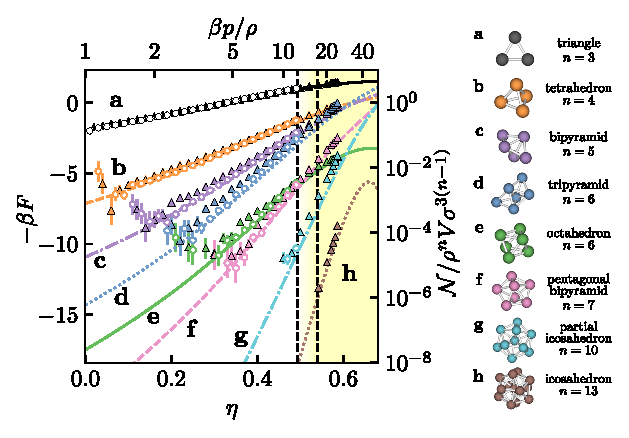
\includegraphics[width=\linewidth,center]{structure-populations}
  \caption[Concentration of local structures in the equilibrium liquid]{
    Static many-body structure in the hard sphere liquid: populations of small local structures in the hard sphere liquid determined from molecular dynamics simulations of 1372 monodisperse (open circles) and 8\% polydisperse (solid triangles) hard spheres against the theoretical prediction of this work (lines).
    Variations against volume fraction $\eta$ and compressibility $Z = \beta p/\rho$ shown.
    The hard sphere freezing and melting volume fractions are indicated by vertical dashed lines.
  }
  \label{fig:structure-populations}
\end{SCfigure}

\begin{SCfigure}
  \includegraphics[width=0.9\linewidth,outer]{n12-dos}
  \caption[Free energy distribution of 12 particle structures]{
    Theoretical free energy distribution for the $n=12$ local library of states at several volume fractions.
    The distribution is shifted to lower energies at higher volume fractions, and develops an increasingly bimodal structure.
    Populations are decomposed into those structures containing pentagonal bipyramids without octahedra (light fill) and the remaining structures (dark fill).
  }
  \label{fig:n12-dos}
\end{SCfigure}

\emph{Existing morphological theories.}---We focus on the hard sphere system because of its fundamental interest in the theory of liquids \cite{WidomS1967,Hansen2013}.
This allows suitable coefficients of Eq.\ \eqref{eq:morphometric-surface-tension} to be derived analytically by exploiting the geometric nature of hard spheres.
We compute morphological quantities and their derivatives following Ref.\ \cite{KleninJCC2011}, which we have extended to calculate curvature measures [see details in the Supplementary Material (SM)].
Note that hard spheres are athermal meaning density is the only control parameter and all free energies are really entropies; here we use ``supercooled'' to mean high density.

We assume the Carnahan-Starling (CS) equation of state \eqref{eq:cs-pressure} \cite{CarnahanJCP1969} because this pressure is used in the WBII theory and is accurate deep within the supercooled regime \cite{BerthierPRL2016} although it will fail at very large densities nearing random close packing.
The pair correlation produced by these coefficients is self-consistent with CS at contact by construction; moreover, the new coefficients provide a theory that outperforms the older WBII approach across the whole range of distances typical of neighbouring particles (SM).
This enables us to accurately model complex many-particle local structures.

\section{Free energy of local structures}

Owing to the high accuracy of the correlations produced with the new morphometric coefficients, we can now calculate many-body correlations in the supercooled regime.
We denote the population of some chosen local structure as $\mathcal{N} = \rho^n V \sigma^{3(n-1)} e^{-\beta F}$, where $F$ is the free energy of the local structure.
From the definition of $g^{(n)}$ as a probability distribution we write the free energy as
\begin{equation}\label{eq:local-structure-free-energy}
  \beta F = -\ln{
    \frac{1}{V \sigma^{3(n-1)}}
    \left(
    \int_{\mathcal{D}}
    g^{(n)}(\vec{r}^n) \, d\vec{r}^n
    \right)
  },
\end{equation}
where the domain of integration $\mathcal{D}$ \emph{defines} the local structure, and $g^{(n)}$ is calculated from the morphometric potential of mean force using Eqs.\ \eqref{eq:potential-mean-force}, \eqref{eq:surface-tension} and \eqref{eq:morphometric-surface-tension} (computational details in SM).
We define a particular local structure by its bond topology, using a pairwise cutoff $\sigma_{cut}$ such that separations between particles are in the range $r_{ij} \in [\sigma, \sigma_{cut}]$ if they are ``bonded'' and $r_{ij} > \sigma$ otherwise.
All results presented use a cutoff of $\sigma_{cut}=1.2 \sigma$, but we have tested our findings are are not significantly affected by a choice of $\sigma_{cut}=1.4 \sigma$ indicating their robustness.

To demonstrate the effectiveness of this approach we have taken rigid structures for $3 \le n \le 13$ which are global minima of clusters in simple liquids \cite{Wales2004}.
We determined their free energies at arbitrary volume fraction by thermodynamic integration (details in SM) of Eq.\ \eqref{eq:local-structure-free-energy}.
In the left panel of Fig.\ \ref{fig:structure-populations} we find excellent agreement between the theoretical prediction and the observed concentration of local structure seen in molecular dynamics simulations of both mono- and moderately polydisperse (8\%) hard spheres at all volume fractions accessed by the simulations i.e.\ $\eta \lesssim 0.585$ (details in SM).

Our approach is able to predict populations of local structures well beyond the regime dynamically accessible to simulation, finding nontrivial structural change deep in the glassy regime highlighted by a rescaling with respect to the trivial $\rho^n$ density contribution.
The free energy of considered structures changes approximately linearly across the entire liquid regime, with deviations from linear becoming more apparent in the supercooled regime.

All structures apart from the fourfold symmetric octahedron in Fig.\ \ref{fig:structure-populations} are subunits of the icosahedron, and increase in concentration more rapidly than the octahedron until high density.
For $n=6$ we consider the free energies of two structures: the tripyramid and octahedron.
We find that the tripyramid occurs $\sim20$ times more often than the octahedron, their free energy difference being dominated by the different point group symmetries following \cite{MalinsJPCM2009,MengS2010}.
We can also estimate vibrational contributions, which allow us to match not only the relative but also the absolute values of free energies obtained from simulation.
In particular, we are able to capture the gradual reduction of the population of octahedral motifs in favour of the tripyramids at high volume fractions.
This is related to the previously observed emergence of fivefold symmetric motifs (such as the full and partial icosahedron) \cite{RoyallPR2015,TarjusJPCM2005,HallettNC2018,DunleavyNC2015}, which is here directly predicted from liquid state theory.

Having tested that the theory is accurate for selected geometries, we now take the exhaustive list of 11980 rigid structures for $n=12$ determined in Ref.\ \cite{Holmes-CerfonSR2016} to obtain a local density of states for a given sized inhomogeneity.
These rigid structures correspond to unique contact topologies, but in thermal systems (i.e. with finite gaps between particles) we expect many of them to be indistinguishable as found in Ref.\ \cite{TrombachPRE2018}.
Nevertheless, because of their exhaustiveness these represent a complete local density of states in the liquid, of fundamental interest to random first-order transition theory \cite{LubchenkoARPC2007}.
We calculated the free energy of all (first-order) rigid (nonsingular) structures using Eq.\ \eqref{eq:local-structure-free-energy} (right panel of Fig.\ \ref{fig:structure-populations}), finding a bimodal distribution with two main peaks separated by a free energy difference that increases with increasing volume fraction.
We find the that lower energy distribution consists of structures rich in fivefold (icosahedral) symmetry in the absence of fourfold (octahedral) symmetry.

\begin{SCfigure}
  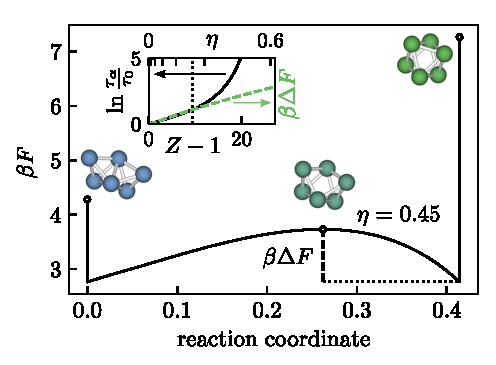
\includegraphics[width=0.9\linewidth,outer]{n6-reaction-path}
  \caption[The simplest nontrivial reaction path in hard spheres: octahedron to tripyramid]{
    Reaction for transition between tripyramid and octahedron $n = 6$ structures.
    Stationary points are indicated by markers: there is a discontinuity in free energy at the end points due to the additional integration over the reaction coordinate, and symmetry in the case of the octahedron.
    Inset: variation of activation barrier with volume fraction $\eta$ and compressibility $Z = \beta p/\rho$ from this theoretical reaction path (dashed line) and measured $\alpha$-relaxation times in bulk molecular dynamics simulations (solid line), where $\eta = 0.45$ is indicated with a vertical dotted line.
  }
  \label{fig:reaction-path-6}
\end{SCfigure}
\todo{Change compressibility factor to pressure}

\todo{Pictures of packings up to n7}

\section{Dynamics: free energy along a reaction path}

We have thus far focused on static thermodynamic properties: yet a connection with dynamics can be made by calculating the free energy along reaction paths between (geometrically similar) structures.
This calculation along unstable directions in the free energy landscape requires an analytic approach (described in the SM), and generates paths such as the one in Fig.\ \ref{fig:reaction-path-6}.
Here we consider transitions between the tripyramid and the octahedron with $n=6$ because this is the simplest nontrivial transition between distinct hard sphere packings (SM).
Comparing this dynamical barrier to the structural relaxation for ($\alpha$-) relaxation timescale $\tau_\alpha$ extracted from simulations relative to a microscopic time $\tau_0$ (inset of Fig.\ \ref{fig:reaction-path-6}), we find this single reaction path barrier agrees with the low density scaling of $\tau_\alpha$ (linear in the compressibility factor $\beta p / \rho$ \cite{BerthierPRE2009}).
However, activated dynamics are not expected in this regime so this agreement may be coincidental.
%Moving to high densities, hard spheres exhibit two-step relaxation when vibrational ($\beta$--) and full ($\alpha$--) relaxations decouple as the system approaches its glass transition \cite{Berthier2011}.
%However, dynamics along the tripyramid--octahedron path continues to increase in an ``Arrhenius'' fashion quite unlike the super-Arrhenius increase exhibited by the $\alpha$--relaxation in the computer simulations (inset of Fig.\ \ref{fig:reaction}).
%It has been shown in molecular systems that $\beta$--relaxation can be Arrhenius in the deeply supercooled regime where $\alpha$-- relaxation is super-Arrhenius \cite{Yu2015}.
%Given that typical particle displacements in the tripyramid--octahedron path are around 0.15$\sigma$ per particle, we observe that this relaxation mechanism may be more characteristic of ($\beta$--) relaxation than full ($\alpha$--) relaxation.
It is possible to extend our methodology for larger rearrangements, which may be sufficient to access ($\alpha$-) relaxation \emph{at very deep supercooling} for equilibrium systems.
However, the rapid growth in the number of possible states presents a considerable numerical challenge requiring new methods and approximations, so we leave this exciting avenue for future study.

\section{Conclusions}

We have presented a formalism for describing many-body correlations in liquids and developed it into an accurate and computationally efficient parameter-free theory for hard spheres using integral geometry relying solely on the choice of the equation of state.
The key approximations involved treating the grand potential as continuous and additive (related to extensivity), and imposing the correct contact value of $g^{(2)}(r)$.

We applied the framework to a selection of local structural correlations, therefore predicting nontrivial changes in the energy landscape with supercooling putting previous empirical observations on more solid ground.
In particular, our analysis provides evidence for the existence of two populations of structures with distinct symmetries and free energies which causes the local density of states to become increasingly bimodal at high densities.
We note that we have treated densities corresponding to a degree of supercooling only accessible using novel swap Monte Carlo techniques \cite{BerthierPRL2016}; however, these simulations introduce large polydispersity, changing the local structure \cite{CoslovichJPCM2018} and thus limiting direct comparison with our calculations for the monodisperse liquid.

Our framework can be easily adapted to more complex liquids such as systems with soft repulsive interactions and polydisperse mixtures \cite{KodamaJCP2011}.
Integral geometry underlies the core equation \eqref{eq:morphometric-surface-tension}, so this approach can extend to hard particles of more complex shapes where the interaction potential is still geometric in nature.
It is applicable to a more general class of liquids where the soft part of the potential may be treated as a perturbation around a hard core \cite{Hansen2013} such that a geometric decomposition still applies.
This suggests a new route for predicting static properties of equilibrium liquids, with direct applications to self-assembly, nucleation and protein structure.

\section{New notes.}

We wish to describe local structure.
Ultimately, we wish to learn about the structure of the energy landscape in hard spheres.
To do so we must characterise the main features of the landscape, namely the different geometric packings and assign weights (free energies) to them.
This is a worthy goal in its own right, perhaps not that interesting for hard spheres but useful for wider applications (e.g.\ predicting self assembly, guiding chemical synthesis, understanding protein folding kinetics and predicting the native state and design).

The path we take is as follows:
\begin{enumerate}
\item We need some means of weighting points in the energy landscape: we do this using the morphometric approach (cf previous chapter)
\item A means of characterising and approximating the entire phase space: energy landscape formalism (next). This has two subgoals:
  \begin{enumerate}
  \item Divide the landscape into stationary points: minima and saddles.
    These stationary points characterise submanifolds of the entire landscape, \emph{basins} in the case of minima and \emph{reaction paths} in the case of saddles.
  \item Integrate over connected manifolds with weight function (potential of mean force) to obtain their free energies.
  \end{enumerate}
\end{enumerate}

%Another way of saying this is we need an integrand and boundary conditions.

\subsection{Connection with energy landscape descriptions}

\begin{itemize}
  \item First describe the energy landscape description.
  \item Based on low-temperature expansion arguments.
  \item Mean-field: Laplace method/saddle-point.
  \item Gaussian expansion around this result (called Harmonic approximation in energy landscape/chemistry literature).
\end{itemize}

\begin{SCfigure}[H]
  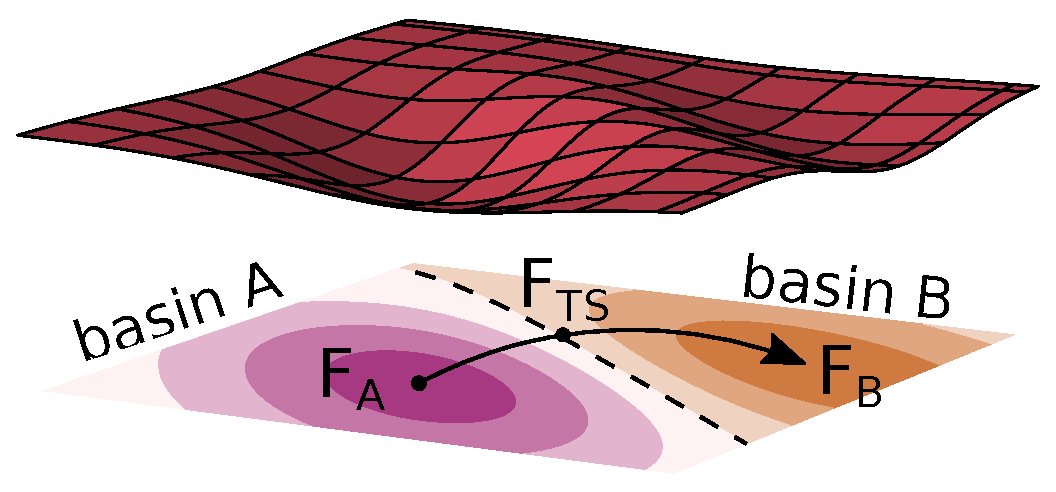
\includegraphics[width=\linewidth,outer]{toy-landscape}
  \caption[A cartoon energy landscape]{A cartoon energy landscape for a 2-dimensional phase space.
    The landscape features two local minima: $A$ and $B$.
    The area surrounding each minima defines its basin: any point from which the minima can be found by moving downhill belongs to the basin.
    Energy landscape approach: at low temperatures the system is expected to oscillate around potential energy minima, so the dynamics can be understood as rare events causing a change of basin.
    Thus a decomposition of the phase space in terms of basins should become exact for the dynamics at low temperatures in the supercooled regime of interest.}
\end{SCfigure}

In the case of local arrangements of hard spheres, rigid packings seem to correspond to minima of the potential of mean force.
I cannot prove this for the case of morphometric approach, but I cannot find a counter example.
Possibly can prove they are minimal volume.

\section{Locally favoured structures in hard spheres}

\subsection{Concentrations of local structure}

How do we define a local structure?
Most of the literature on structure in amorphous systems falls into one of either two categories
Almost all methods for Common methods:
\begin{itemize}
  \item Bond orientational order parameters
  \item Bond networks: take some bond detection algorithm (voronoi, 
Fom the partition function of the potential of mean force
Suppose we have a definition of a
\end{itemize}

From the definition of the probability density function in Eq.\ \eqref{eq:n-density-pdf}, the total number of local structures of a particular type in a volume $V$ is
\begin{equation}\label{eq:structure-population}
  \mathcal{N} =
  \int_{\mathcal{Q}} \rho^n g^{(n)}(\vec{r}^n) \, d\vec{r}^n,
\end{equation}
where $\mathcal{Q}$ is the domain \emph{defining} the local structure.
To get the free energy expression used in the main text we consider the manifold diffeomorphic to translations, defining $\mathcal{Q} = \mathcal{D} \rtimes \mathbb{V}$ where $\mathbb{V}\subset \mathbb{R}^3$ is the system volume.
Exploiting translational invariance of the potential of mean force, we fix one particle at the origin and integrate the center of mass over the system volume giving
\begin{equation}
  \mathcal{N} =
  \rho^n V \int_{\mathcal{D}} g^{(n)}(\vec{r}^n) \, d\vec{r}^{n-1}.
\end{equation}
We defined a free energy by taking $\mathcal{N} = \sigma^{3(n-1)} \rho^n V e^{-\beta F}$, which together with the above expression gives Eq.\ \eqref{eq:local-structure-free-energy} in the main text.

More generally, we consider the manifold diffeomorphic to translations \emph{and} rotations.
We define $\mathcal{Q} = \mathcal{D}' \rtimes SE(3)$ where $\textrm{SE}(d)$ is the $d$-dimensional special Euclidean group, leaving the $\mathcal{D}'$ as the space of the structure's internal motion.
\todo{Make this consistent with the notation of background chapter.}
We separate rigid body from internal motion by applying the following transformation to each particle coordinate
\begin{equation}
  \vec{r}(\{\vec{t}, \vec{\theta}, \vec{x}\}) =
  \vec{t} + \vec{R}(\vec{\theta}) \cdot \vec{q}(\vec{x}),
\end{equation}
where $\vec{t}$ is the translation vector, $\vec{\theta}$ the Euler angles, $\vec{R}$ the rotation matrix, and $\vec{x} \in \mathbb{R}^{3n-6}$ represents the internal coordinates.
We need to compute the metric of this transformation $G_{ij} = \vec{G}_i \vec{G}_i^T$ where the (generally curvilinear) basis vectors are $\vec{G}_i = \partial_i \vec{r}$.
To simplify calculation we choose $\vec{q}(\vec{x})$ to always be in the center-of-mass frame and orthogonal to rotations such that $G_{ij}$ reduces to block-diagonal form.
If the rotation matrix is expressed in Euler-angle representation as $\vec{R}(\vec{\theta}) = \vec{R}_3(\theta_3) \vec{R}_2(\theta_2) \vec{R}_1(\theta_1)$ then we have%
\marginfootnote{There is no elegent omitted step to obtain the form of $\vec{U}$ which gives the block diagonal form; rather, I used a series of educated guesswork within Mathematica to obtain this.
  There is probably a more direct route.}
\begin{equation}
  \vec{G}(\vec{\theta}, \vec{x}) =
  \begin{pmatrix}
    n \vec{E} & 0 & 0 \\
    0 & \vec{U}^T(\vec{\theta}) \vec{I}(\vec{x}) \vec{U}(\vec{\theta}) & 0 \\
    0 & 0 & \overline{\vec{G}}(\vec{x})
  \end{pmatrix},
\end{equation}
where $\vec{E}$ is the identity matrix, $\overline{\vec{G}}$ is the metric for internal motion, and we have defined the matrix $\vec{U}$ as
\begin{equation}
  \vec{U}(\vec{\theta}) =
  \begin{pmatrix}
    1 &  0              & -\sin{\theta_2} \\
    0 &  \cos{\theta_1} &  \cos{\theta_2} \sin{\theta_1} \\
    0 & -\sin{\theta_1} &  \cos{\theta_2} \cos{\theta_1} \\
  \end{pmatrix}
  \qquad
  \begin{aligned}
    \theta_1 &\in [0,2\pi] \\
    \theta_2 &\in \left[-\frac{\pi}{2},\frac{\pi}{2}\right] \\
    \theta_3 &\in [0,2\pi].
  \end{aligned}
\end{equation}
Note $\det{\vec{U}} = \cos{\theta_2}$.
The volume element in the new coordinates is
\begin{equation}
  d\vec{r}^n = \frac{\sqrt{\det G_{ij}(\vec{x})}}{\nu}
  \, d^3 \vec{t} \, d^3 \vec{\theta} \, d^{3n-6} \vec{x},
\end{equation}
where $\nu$ is the symmetry number (discussed below) and
\begin{equation}
  \sqrt{\det G_{ij}(\vec{x})} =
  \cos{\theta_2} \sqrt{\det{\vec{I}(\vec{x})}}
  \sqrt{n^3 \det{\overline{G_{ij}}(\vec{x})}}.
\end{equation}
The symmetry number emerges as the choice of internal coordinates typically fixes the particle labels breaking permutation symmetry; we have to multiply by the $n!$ possible labellings, which introduces double counting if the structure possesses rotational symmetry so we have to divide by the correcting factor $\nu$.
This is explained in detail in Ref.\ \cite{CatesSM2015}.
Thus \eqref{eq:structure-population} reduces to
\begin{equation}\label{eq:structural-partition-function-detailed}
  \frac{\mathcal{N}}{\rho^n V}
  =
  \frac{8\pi^2 \sqrt{n^3}}{\nu} \int_{D'}
  g^{(n)}(\vec{x}) \,
  \sqrt{\det{\overline{G_{ij}}(\vec{x})} \det{\vec{I}(\vec{x})}}
  \, d^{3n-6} \vec{x}.
\end{equation}
Note that in the limit of linear molecules, i.e.\ where all particles fall on a line, the above approach fails as there is one less rotation mode requiring a modified description.

In general, the integrand in \eqref{eq:structural-partition-function-detailed} is only exactly solvable for the simplest geometries due to the high dimensionality of $\vec{x}$.
This is further complicated by the fact that the basis vectors for $\overline{G_{ij}}$ are curvilinear.
We use two methods for evaluating these integrands:
\begin{enumerate}
\item Monte Carlo simulation: described in the next section.
\item Analytically via perturbation theory: described in sections \ref{SI:bond-distance} and \ref{SI:reaction-path}.
  We use this for a similar integrand along a reaction path where Monte-Carlo cannot be used directly.
\end{enumerate}

\subsection{Bond-distance space}
To evaluate the integrand in Eq.\ \eqref{eq:structural-partition-function-detailed} analytically we need to choose a representation for $\vec{x}$ which is diffeomorphic to $\vec{r}^n$.
For \emph{minimally constrained geometries}, i.e.\ structures with exactly $3n-6$ contacts, a convenient representation exists: bond distance space.
Following Ref.\ \cite{Holmes-CerfonPNAS2013} and its accompanying Supplementary Information we choose each element of $\vec{x}$ to represent the distances between particles in contact, where contact occurs at $\vec{x} = (\sigma, \dots, \sigma)$.
Thus increasing elements of $\vec{x}$ corresponds to thermal fluctuations away from contact.
This representation naturally expresses the limits of integration given in the main text as $\sigma \le x_i \le \sigma_{cut}$.

To evaluate the integral we need expressions for the internal metric and moment of inertia terms.
The internal metric is defined in terms of the Jacobian matrix $\vec{J} \in \mathbb{R}^{3n \times 3n-6}$
\begin{equation}
  \overline{G_{ij}} = \vec{J}^T \vec{J}
\end{equation}
where the matrix entries are given by
\begin{equation}
  J_{ij} = \frac{\partial q_i}{\partial y_j}.
\end{equation}
In practice it is easier to calculate its inverse numerically (via finite differences) using
\begin{equation}
  J_{ij}^{-1}
  = \frac{\partial y_j}{\partial q_i}
  = \left. \frac{\partial y_j}{\partial x_i}
  \right|_{\vec{\theta} = \vec{t} = \vec{0}}
\end{equation}
which has linearly independent rows for a minimally constrained geometry so we recover $\vec{J}$ from $\vec{K} = \vec{J}^{-1}$ using the matrix inversion formula $\vec{J} = (\vec{K}^T\vec{K})^{-1} \vec{K}^T$.
The above expressions all depend implicitly on the point $\vec{x}$ as the coordinate scheme is curvilinear, so to keep the integral tractable we approximate this to leading order as
\begin{equation}
  \sqrt{\overline{G_{ij}}(\vec{x})} \simeq \sqrt{\overline{G_{ij}}(\vec{x}_0)}
\end{equation}
where $\vec{x}_0 = (\sigma,\dots,\sigma)$ is contact.
Thus the integral becomes
\begin{equation}\label{eq:structural-partition-function-approximated}
  \frac{\mathcal{N}}{\rho^n V}
  =
  \frac{8\pi^2 G_0}{\nu} \int_{D'}
  g^{(n)}(\vec{x}) \,
  \sqrt{\det{\vec{I}(\vec{x})}}
  \, d^{3n-6} \vec{x}
\end{equation}
where $G_0 = \sqrt{n^3 \det{\overline{G_{ij}}(\vec{x}_0)}}$.

Finally, we write the distribution function in terms of the potential of mean force and expand this and the moment of inertia to first order, as in
\begin{align}
  \phi^{(n)}(\vec{x}) &=
  \phi^{(n)}(\vec{x}_0) +
  (\vec{x} - \vec{x}_0) \cdot
  \left. \vec{\nabla} \phi^{(n)}(\vec{x}) \right|_{\vec{x} = \vec{x}_0} +
  \mathcal{O}(\vec{x}^2), \\
  \sqrt{\det{\vec{I}(\vec{x})}} &=
  \sqrt{\det{\vec{I}(\vec{x}_0)}} +
  (\vec{x} - \vec{x}_0) \cdot
  \left. \vec{\nabla} \sqrt{\det{\vec{I}(\vec{x})}} \right|_{\vec{x} = \vec{x}_0} +
  \mathcal{O}(\vec{x}^2).
\end{align}
Using the analytical gradient expressions given in Section \ref{SI:line-curvature} makes this calculation very efficient.
The integral \eqref{eq:structural-partition-function-approximated} separates into $3n-6$ independent one-dimensional integrals of the form
\begin{equation*}
  \int_\sigma^{\sigma_{cut}} (a_i + b_i x_i) e^{-c_i x_i} dx_i
  = \left[
    - \left(
    \frac{(a + b_i x_i)}{c_i} + \frac{b_i}{c_i^2} \right) e^{-c_i x_i}
  \right]_\sigma^{\sigma_{cut}},
\end{equation*}
where $a_i$, $b_i$ and $c_i$ are constants.

Loosely speaking, this is the hard-particle analogue of the harmonic approximation with the difference here being that the first derivative does not vanish at the minimum.
For $n=6$ this expansion works rather well, as all structures have exactly $3n-6$ bonds and this perturbation theory captures the free energy well when compared with the ``exact'' result from thermodynamic integration.

\section{Introduction}

This study builds on and contributes to work in nonequilibrium statistical physics, particularly relating to glasses and nucleation.
Although small-system studies have examined how dynamics are influenced by topographical properties of the energy landscape for simple systems, there has not been a systematic formalism for extending this to the bulk liquid.
As such, this study provides additional insight into dynamical arrest i.e.\ the supercooled liquid and glasses.

The analytic focus on many-body correlations provides another contribution to the fundamental understanding of simple liquids.
This study analyses depletion forces in order to predict the many-body correlation functions in the bulk liquid.
Although numerous studies have identified the role of local structure in dynamical arrest little analytical attention has been paid to how to properly formulate structure in a quantitative thermodynamic framework.
I address this issue by expressing the solvation free energies in terms of geometrical properties of a small solute, and develop techniques for making quantitative predictions of local structure in the hard sphere liquid.

Energy landscape can be divided into two strands: the topographic view of Stillinger which offers a powerful conceptual tool for understanding complex phenomena.
At low temperatures we can imagine the system oscillating around low energy minima (inherent states), with occasional large fluctuations driving it through `choke points' causing a change to a different energy minimum.
This formalism was turned into a properly quantitative framework by Wales \cite{Wales2004,?}, where stationary point databases are constructed: energy minima connected by saddles.
From the connectivity of the landscape one can understand dynamical arrest: if there are lots of competing low lying minima it can be hard for the system to find the global minimum and we expect it to fall out of equilibrium easily when temperature is lowered.
By contrast, if the minima steadily lower in energy then they act as a funnel to the global minimum so we expect rapid equilibration.

Quantitative predictions are typically only possible for small systems, so it is desirable to extend it to the bulk.
One can to do this focusing on a subset of the total degrees of freedom, integrating out the rest in an approximate fashion.
The selected degrees of freedom act as a small system with a many-body interaction potential, so can be treated with the aforementioned formalism in a quantitative manner.
This was attempted by Tarjus \cite{?} with mixed success.
The morphometric approach \cite{KonigPRL2004,RothPRL2006,RobinsonPRL2019} offers a generic framework to treat many-body correlations allowing a first-principles treatment of local structure in the bulk liquid.
This framework is accurate for hard spheres where it has been extensively tested \cite{Hansen-Goos?,Roth?,Bob?,RobinsonPRL2019}.

Hard particle systems are the fundamental system of interest for simple liquids.
The stationary point database approach, firmly rooted in \emph{potential energy}, fails for hard systems as the potential energy is trivial so the thermodynamics is athermal.
It has never been extended to hard systems until now.
This extension comes with the cost that some of the elegant techniques of soft systems will fail due to the singular nature of hard sphere interactions, so we require new methods to handle the idiosyncrasies of hard systems.
Here we propose a practical definition for basins when working with hard systems, and develop techniques for evaluating thermodynamic quantities with this definition.
We then retroactively justify the meaningfulness of this basins by comparing with simulation/literature data.

\todo{Talk about the past work on hard spheres: penny packing, and sticky spheres.}
A number of unique technical challenges brought about by the hard sphere potential, that we will solve.
The groundwork for this was laid down by Holmes-Cerfon and coworkers.
Note: attempts have been successful at modelling effective interactions close to isostaticity where $z \to 2d$.
This is empirically found to be the case asymptotically as one approaches jamming, however it is worth noting that there is no general requirement that $z = 2d$ for rigid packings, and counter examples where $z < 2d$ are known.

In section \ref{sec:energy-landscapes} we review the energy landscape formalism for soft potentials, with a view to highlighting where it might fail for hard interactions.
We review the liquid state theory/morphological approach used for treating the depletion interactions between hard particles in the bulk liquid in section \ref{?},
followed by the equivalent of the partition function for local structure.
Our core theoertical results are then presented in section \ref{?}, where we propose a definition of local structure and show techniques for evaluating the partition function nonperturbatively.
We then present the results of the topography of the local structural energy landscape in hard spheres in section \ref{?}, our main numerical results.

\section{Energy landscape approaches}
\label{sec:energy-landscapes}

Points to cover:
\begin{itemize}
\item Give a technical definition of local structure with a goal to showing the problems with hard systems.
\item Define structures as manifold: $\mathbb{R}^{dn}$ for $n \ll N$, embedded in $\mathbb{R}^{dN}$
\item Failure of perturbation theory due to singularity of 
\end{itemize}

The energy landscape/inherent structure approach is a powerful theoretical framework for understanding complex phenomena.
At its core, it is a means of coarse-graining the high dimensional phase space into a more manageable mesostates.
Its power comes from the fact that it is essentially exact, though calculations are typically intractable unless the degrees of freedom can be significantly reduced; in practice this is generally only possible in mean field (high spatial dimensions) or for small systems $N = \mathcal{O}(10)$ in physical settings.
The approach is however useful conceptually for developing theories based around the topography of the energy landscape \cite{Stillinger}, and makes detailed calculations tractable typically for small systems \cite{Wales2004}.

In this section we will review the energy landscape approach, how it applies to soft potentials and the complications that arise for our system of interest: hard spheres.
First we talk about coarse-graining into mesostates mentioned above, whether into inherent structures or otherwise.
A mesostate is a collection of microstates which are grouped together, typically these are selected for sharing some desirable property to simplify description.
For practical reasons this means that microstates should be connected in phase space so they are compact manifolds.
In connection with the topographic view we will call these manifolds \emph{basins}.
The total partition function is then decomposed as
\begin{equation}
  Z \equiv \int_{\mathbb{R}^{dN}} e^{-\beta (U_N(\vec{r}^n) + \phi(\vec{r}^n))} \, d\vec{r}^N = \sum_i Z_i
\end{equation}
where $\phi$ is the external potential of the container in order to keep the particles localised in a region where they interact.
Alternatively they could be embedded in a toroidal topology to prevent particle dissociation (as in e.g.\ simulations with periodic boundary conditions).
The basin partition function is
\begin{equation}
  Z_i = \int_{\mathbb{V}_i^{dN}} e^{-\beta U_N(\vec{r}^N)} \, d\vec{r}^N
\end{equation}
if $\mathbb{V}_i^{dN} \subset \mathbb{R}^{dN}$ is the manifold corresponding to basin $i$.
One can define (e.g.\ Wales).
Despite a definition which unambiguously demarcates the basins, the high dimensionality of the phase space renders the integrals in \eqref{eq:basin-partition-function} completely intractable without approximation.

The equilbrium probability of the system being in basin $i$ at any one time is thus
\begin{equation}
  p_i = \frac{Z_i}{Z}
\end{equation}
From the Gibbs-Shannon entropy we find the coarse-graining entropy
\begin{equation}
  \begin{split}
    S_{\textrm{conf}}
    &= -\sum_i p_i \ln{p_i} \\
    &= -\sum_i \left( \frac{Z_i}{Z} \ln{Z_i} - \frac{Z_i}{Z} \ln{Z} \right) \\
    &= \ln{Z} - \sum_i \frac{Z_i}{Z} \ln{Z_i}
  \end{split}
\end{equation}
Noting that the total free energy is $F = -k_B T \ln{Z}$ we thus have
\begin{equation}
  \beta F = \langle \beta F_i \rangle - S_{\textrm{conf}}
\end{equation}
where the average basin free energy $F_i = -k_B T \ln{Z_i}$ is
\begin{equation}
  \langle \beta F_i \rangle = - \frac{1}{Z} \sum_i Z_i \ln{Z_i}
\end{equation}

Finally, we have to choose how to define the basins.
In the energy landscape approach the coarse-graining occurs around local minima of energy where $\vec{\nabla}U_N = 0$ and Hessian $\frac{1}{2}\vec{\nabla}\vec{\nabla}U_N$ is positive definite.
Each basin consists of all the points connected by a steepest descent path to a unique energy minimum.
This description reduces the high dimensional continuous description down to discrete number of zero-dimensional manifolds.
In practice the number of minima scales exponentially in $N$, so this is still an intractably large number of points.
One can even obtain dynamical information by considering the saddles, i.e.\ the unstable stationary points.
The saddles act as the lowest (in energy) lying points that must be crossed to jump from one basin to another, giving the energy barriers to dynamics.

How do we justify this approach?
Energy is smooth so asymptotics around stationary points is valid: inherent state (stable stationary points) description
For infinite systems we could use Laplace method
\begin{equation}
  \int_{\mathbb{V}^{dN}_i} e^{-\beta N u_N(\vec{r}^N)} \, d\vec{r}^N
  \sim
  e^{-\beta \min{U_N(\vec{r}^N)}} \qquad \forall \; N \gg 1
\end{equation}
where $u_N = U_N / N$.
For finite systems we could go beyond this pertubatively by employing a harmonic approximation from the energy-landscape literature
\begin{equation}
  U_N = U_N(\vec{p}_i) +
  \frac{1}{2} \Delta \vec{r} \cdot \left. \nabla \nabla U_N\right|_{\vec{p}_i} \cdot \Delta \vec{r}
  + \mathcal{O}(\Delta \vec{r}^3)
\end{equation}
where \[\vec{p}_i = \argmin_{\vec{r}^n \in \mathbb{V}_i^{dN}}{\left(U_N(\vec{r}^n)\right)}\] is the location of the energy minimum.
\begin{equation}
  Z_i \sim \exp{-\beta U_N(\vec{p}_i)}
\end{equation}
There are two layers of approximation: first we model the pdf as a Gaussian, second we approximate the boundary conditions as being infinite.
The inclusion of the Hessian term in the expansion around the minimum shows that for soft potentials one can perturbatively build a description around the inherent states.
At low temperatures this approach is expected to become exact (for the first layer not the second one).
So for athermal systems perturbation theory should break down.

\begin{SCfigure}
  \missingfigure[figwidth=\linewidth]{}
  \caption{Failure of Laplace method for hard interactions.}
\end{SCfigure}

To make the above discussion concrete we will consider two examples.
First, we examine a symmetric quartic potential
\begin{equation}
  \phi = \epsilon (x^4 - x^2)
\end{equation}
where $x$ is some state variable and $\epsilon$ is an energy scale.
This could represent e.g.\ a ferromagnet below the critical temperature with $x$ representing the spontaneous magnetisation.
The free energy in units of $\epsilon$ is then
\begin{equation}
  F = - T \ln{\left( \int \exp{\left(-\frac{\phi}{T}\right)} \, dx \right)}
\end{equation}
This potential naturally contains two basins for the two half space $x \in [-\infty, 0]$ and $x \in [0, \infty]$, and because of the symmetry of the potential around $x=0$ the contribution of each of these basins is identical, i.e.\
\begin{equation}
  Z = 2 \int_0^\infty \exp{\left(-\frac{\phi}{T}\right)} \, dx.
\end{equation}
Applying the harmonic approximation
\begin{equation}
  \begin{split}
  Z &\simeq
  2 \exp{\left( -\frac{\phi(x_0)}{T} \right)}
  \int_{-\infty}^\infty \exp{\left(-\frac{\phi''(x_0)}{2T}\right)} \, dx \\
  &=
  2 \exp{\left( -\frac{\phi(x_0)}{T} \right)}
  \sqrt{\frac{2 \pi T}{\phi''(x_0)}}
  %+ \mathcal{O}(\phi'''(x_0))
  \end{split}
\end{equation}
where $x_0 = \dfrac{1}{\sqrt{2}}$ is the position of the minimum in the $x > 0$ basin.

The hard sphere potential is a pathological case: the singularity in the pair potential dooms harmonic treatments.
To illustrate this, we consider a worked example.
Consider as a worked example two one-dimensional particles interacting via a repulsive inverse power law $u_{\textrm{pair}}(r) = \epsilon r^{-\gamma}$ for $\gamma > 1$ where $\epsilon > 0$ is the interaction energy, and depletion interactions modelled as a linear term $u_{\textrm{depletion}}(r) = r$.
This toy model approximately corresponds to the small $r$ behaviour close to contact for 3d hard spheres Fig.\ \ref{?}.
The partition function is
\begin{equation}
  %\begin{split}
  Z(\gamma)
  = \int_1^{\infty} \exp{\left(-\frac{\epsilon}{r^\gamma}\right)} \, dr
  = \left[ \frac{r^{1-\gamma}}{1-\gamma} \right]_1^\infty
  = \frac{1}{\gamma - 1}
  %\end{split}
\end{equation}
The free energy is thus
\begin{equation}
  F(\gamma) = \ln{(\gamma - 1)}
\end{equation}
which is a finite quantity for all $r$.
If we compare this against the harmonic approximation, however, we obtain
\begin{equation}
  F(\gamma) \propto \gamma(\gamma - 1)
\end{equation}
which diverges in the hard sphere limit $\gamma \to \infty$.
The hard sphere limit is properly singular, and we must use nonperturbative methods to treat it.
We will however take inspiration of the approach for soft potentials, and hope to adapt these into a framework for doing similar calculations.

To summarise this section, we note that the basin definition of structures for soft potentials has the properties that: \cite{Wales?}
\begin{itemize}
\item Each basin $B_i$ connects to a unique minimal energy state with a unique geometry.
\item Divide the phase space into basins which do not overlap $B_i \cap B_j = \emptyset$ for $i \ne j$ and tile the whole of phase space $\cup_i B_i = \mathbb{R}^q$.
\item Its free energy is well-defined (at least in some asymptotic limit) so it can be approximated with simple methods.
  For soft potentials this is a consequence of the first criterion.
  This makes the choice of coarse-graining (thermo)dynamically meaningful: it is long-lived enough that the microstates making up a basin can be not distinguished, and the dynamics reduces to basin crossing events.
\end{itemize}
A definition satisfying the first two criteria is possible, however due to the singularity in the hard particle interaction potential the region surrounding the (depletion) energy minimum is thermodynamically irrelevant.
This can be interpretted:
\begin{itemize}
\item \emph{Thermodynamically}: the region near contact is entropically suppressed, regions away from contact have many more microstates so are entropically enhanced
\item \emph{Dynamically}: as hard spheres approach one another they collide and bounce away so spend infinitesimally small timescales at contact.
  Collisions almost universally involve only two particles, collisions of more than two particles occur with zero measure.
\end{itemize}
Because of this we cannot obtain the free energy by a small parameter expansion around the contact point.
We must evaluate the full integral over a finite volume.
To make this tractable we will abandon the rigorous definition of structures in terms of basins employed for soft potentials, in favour of a simple one based on intuitive geometrical ideas.
We will later explore the limitations/successes of this definition in order to retroactively justify this approach.

Due to the analogies between the population/concentration integral and the usual partition function, we will refer to this integral simply as a partition function.

\subsection{Molecular partition function}

From the definition of the probability density function in Eq.\ \eqref{eq:n-density-pdf}, the total number of local structures of a particular type in a volume $V$ is
\begin{equation}\label{eq:structure-population}
  \mathcal{N} =
  \int_{\mathcal{Q}} \rho^n g^{(n)}(\vec{r}^n) \, d\vec{r}^n,
\end{equation}
where $\mathcal{Q}$ is the domain \emph{defining} the local structure.
To get the free energy expression used in the main text we consider the manifold diffeomorphic to translations, defining $\mathcal{Q} = \mathcal{D} \rtimes \mathbb{V}$ where $\mathbb{V}\subset \mathbb{R}^3$ is the system volume.
Exploiting translational invariance of the potential of mean force, we fix one particle at the origin and integrate the center of mass over the system volume giving
\begin{equation}
  \mathcal{N} =
  \rho^n V \int_{\mathcal{D}} g^{(n)}(\vec{r}^n) \, d\vec{r}^{n-1}.
\end{equation}
We defined a free energy by taking $\mathcal{N} = \sigma^{3(n-1)} \rho^n V e^{-\beta F}$, which together with the above expression gives Eq.\ \eqref{eq:local-structure-free-energy} in the main text.

There will be $d$ translation modes and $\frac{d(d-1)}{2}$ rotational modes for each plane formed by pairs of coordinate axes (e.g.\ $x^1 \wedge x^2$ for rotations in the $x^1x^2$-plane).
Subtracting the number of rigid body modes from the total degrees of freedom gives \[ q = dn - \frac{d(d+1)}{2} \] internal degrees of freedom.
Exception when rotations are degenerate: $n < d$ (e.g.\ $n=2$ in $d=3$) or pathological cases of unusually high symmetry (e.g.\ when all particles fall on a line) which can in general be excluded.

More generally, we consider the manifold diffeomorphic to translations \emph{and} rotations.
We define $\mathcal{Q} = \mathcal{D}' \rtimes SE(3)$ where $\textrm{SE}(d)$ is the $d$-dimensional special Euclidean group, leaving the $\mathcal{D}'$ as the space of the structure's internal motion.
We separate rigid body from internal motion by applying the following transformation to each particle coordinate
\begin{equation}
  \vec{r}(\{\vec{t}, \vec{\theta}, \vec{x}\}) =
  \vec{t} + \vec{R}(\vec{\theta}) \cdot \vec{q}(\vec{x}),
\end{equation}
where $\vec{t}$ is the translation vector, $\vec{\theta}$ the Euler angles, $\vec{R}$ the rotation matrix, and $\vec{x} \in \mathbb{R}^{3n-6}$ represents the internal coordinates.
We need to compute the metric of this transformation $G_{ij} = \vec{G}_i \vec{G}_i^T$ where the (generally curvilinear) basis vectors are $\vec{G}_i = \partial_i \vec{r}$.
To simplify calculation we choose $\vec{q}(\vec{x})$ to always be in the center-of-mass frame and orthogonal to rotations such that $G_{ij}$ reduces to block-diagonal form.
If the rotation matrix is expressed in Euler-angle representation as $\vec{R}(\vec{\theta}) = \vec{R}_3(\theta_3) \vec{R}_2(\theta_2) \vec{R}_1(\theta_1)$ then we have%
\footnote{While the final form of $\vec{G}$ is elegant, I do not have a straightforward way of getting it; it involved a lot of guesswork and within Mathematica to find a form of $\vec{U}$ which gives the middle block.
  There is probably a more direct route.}
\begin{equation}
  G_{ij}(\{\theta_i\}, \vec{x}) =
  \begin{pmatrix}
    n \vec{E} & 0 & 0 \\
    0 & \vec{U}^T(\vec{\theta}) \vec{M}(\vec{x}) \vec{U}(\vec{\theta}) & 0 \\
    0 & 0 & \overline{G_{ij}}(\vec{x})
  \end{pmatrix},
\end{equation}
where $\vec{E}$ is the identity matrix, $\vec{M}$ is the moment of inertia tensor, $\overline{G_{ij}}$ is the metric for internal motion, and we have defined the matrix $\vec{U}$ as
\begin{equation}
  \vec{U}(\vec{\theta}) =
  \begin{pmatrix}
    1 &  0              & -\sin{\theta_2} \\
    0 &  \cos{\theta_1} &  \cos{\theta_2} \sin{\theta_1} \\
    0 & -\sin{\theta_1} &  \cos{\theta_2} \cos{\theta_1} \\
  \end{pmatrix}
  \qquad
  \begin{aligned}
    \theta_1 &\in [0,2\pi] \\
    \theta_2 &\in \left[-\frac{\pi}{2},\frac{\pi}{2}\right] \\
    \theta_3 &\in [0,2\pi].
  \end{aligned}
\end{equation}
Note $\det{\vec{U}} = \cos{\theta_2}$.
The volume element in the new coordinates is
\begin{equation}
  d\vec{r}^n = \frac{\sqrt{\det G_{ij}(\vec{x})}}{\nu}
  \, d^3 \vec{t} \, d^3 \vec{\theta} \, d^{3n-6} \vec{x},
\end{equation}
where $\nu$ is the symmetry number (discussed below) and
\begin{equation}
  \sqrt{\det G_{ij}(\vec{x})} =
  \cos{\theta_2} \sqrt{\det{\vec{M}(\vec{x})}}
  \sqrt{n^3 \det{\overline{G_{ij}}(\vec{x})}}.
\end{equation}
The symmetry number emerges as the choice of internal coordinates typically fixes the particle labels breaking permutation symmetry; we have to multiply by the $n!$ possible labellings, which introduces double counting if the structure possesses rotational symmetry so we have to divide by the correcting factor $\nu$.
This is explained in detail in Ref.\ \cite{CatesSM2015}.
Thus \eqref{eq:structure-population} reduces to
\begin{equation}\label{eq:structural-partition-function-detailed}
  \frac{\mathcal{N}}{\rho^n V}
  =
  \frac{8\pi^2 \sqrt{n^3}}{\nu} \int_{D'}
  g^{(n)}(\vec{x}) \,
  \sqrt{\det{\overline{G_{ij}}(\vec{x})} \det{\vec{M}(\vec{x})}}
  \, d^{3n-6} \vec{x}.
\end{equation}
Note that in the limit of linear molecules, i.e.\ where all particles fall on a line, the above approach fails as there is one less rotation mode requiring a modified description.

Note that for all of the geometries we have tested this metric seems to be 2, although we could not prove this is in the general case.
We have to actually evaluate the integral.
We will explore thermodynamic integration using Monte Carlo, which is essentially exact to numerical precision but slow, and some analytical approximations.

\subsection{Worked examples}

%% \begin{SCfigure}
%%   \missingfigure[figwidth=\linewidth]{}
%%   \caption{Number of first shell neighbours in the hard sphere liquid.}
%% \end{SCfigure}

%% \begin{SCfigure}
%%   \missingfigure[figwidth=\linewidth]{}
%%   \caption{Number of equilateral triangles in the hard sphere liquid.}
%% \end{SCfigure}

We will consider two worked examples for simple geometries which are readily visualised and for which the metric $G(\vec{x})$ is known exactly and the partition function integral reduces to a simple form.

Our first worked example is at the two-body level: the typical number of neighbours in the first shell.
For a dimer the metric term evaluates to $G(\vec{x}) = r^2$, i.e.\ the usual spherical coordinate Jacobian as expected.
The average number neighbours less than some distance $r$ is then
\begin{equation}
  z(r)
  = 4\pi \int_0^r g^{(2)}(r) r^2 \, dr
  = 4\pi \int_\sigma^r e^{-\beta \phi^{(2)}(r)} r^2 \, dr
\end{equation}
This is a common measurement where $r$ is taken up to the first minimum of the $g(r)$ then $z$ corresponds to the number in the ``first-shell'' (i.e. the coordination number).

Our second worked example considers the average concentration of triangles in the liquid.
Here the relevant coordinates are the tuple $\vec{x} = (r,s,t)$ where the three distances are the lengths of the triangle.
The metric has previously been determined exactly as $G(\vec{x}) = rst$ in \cite{?}.
The number of equilateral triangles with maximum side length $\delta$ is then
\begin{equation}
  N_\Delta(\delta)
  =
  8\pi^2 \int_\sigma^\delta\int_\sigma^\delta\int_\sigma^\delta
  e^{-\beta\phi^{(3)}(r,s,t)} rst \, dr ds dt.
\end{equation}
The results show excellent agreement with molecular dynamics simulations across the entire liquid regime, and even into the supercooled regime where simulations are available for a polydisperse system.

\subsection{Exact result: thermodynamic integration}

\todo{State that we want the saddles: they are the primary reason for developing analytical methods}

Before moving on to our approximate analytical integration schemes we describe a method which is essentially exact to within numerical precision, at the cost of greater computational expense.
We will use thermodynamic integration to test the accuracy of our analytical methods.
Aspects of this method were inspired by Ref.\ \cite{SchillingJCP2009}.
As a Monte-Carlo method it would be very difficult to extend this method to saddles which is of great interest.

We perform a thermodynamic integration between two potentials $V_1$ and $V_2$ by considering the intermediate potential
\begin{equation}
  V(\vec{r}^n; V_1, V_2) = \lambda V_1(\vec{r}^n) + (1-\lambda) V_2(\vec{r}^n).
\end{equation}
where $\lambda \in \{0,1\}$ is a mixing parameter.
Over the course of a Monte-Carlo sweep, in addition to regular steps $\lambda$ is allowed to switch between these values according to the Metropolis-Hastings rule.
The free energy difference between the two systems is determined from the ratio of time spent with each potential active by
\begin{equation}
  \Delta F \equiv F_2 - F_1 = -\log{\left( \frac{t_2}{t_1} \right)},
\end{equation}
where $t_i$ is the total number of sweeps where potential $i$ is active (by $\lambda$ value).

Local structure is defined in the main text by its bond topology.
We define an $n \times n$ adjacency matrix $\mathcal{A}$ giving the bond topology of $n$ particles by
\begin{equation}
  A_{ij} =
  \begin{cases}
  1 \quad i \textrm{ and } j \textrm{ ``bonded''} \\
  0 \quad \textrm{otherwise}
  \end{cases}
\end{equation}
The hard core interaction ensures $r_{ij} \equiv |\vec{r}_i - \vec{r}_j| > \sigma$ for all $(i,j)$ including non-bonded particles, but the ``bonded'' flag forces the stricter condition that $r_{ij} \in [\sigma, \sigma_{cut}]$ when $A_{ij} = 1$.
The latter strict criterion is how we are able to focus on specific local structures.

To do the thermodynamic integration we introduce an intermediate potential which takes into account the boundary conditions of the integral:
\begin{equation}
  \phi(\vec{r}^n; v_\lambda, \eta) =
  \sum_{i < j} A_{ij} v_\lambda(r_{ij})
  + \phi^{(n)}(\vec{r}^n; \eta)
\end{equation}
where $v_\lambda$ is a \emph{confining} potential to restrict the Monte-Carlo to integrate only the structure of interest.
We have indicated the dependence of the potential of mean force on volume fraction, noting that in the ideal gas limit the grand potential (solvation) term vanishes leaving only the potential energy contribution
\begin{equation}
  \phi^{(n)}(\vec{r}^n; \eta=0) = \sum_{i < j} v_{hs}(r_{ij}),
\end{equation}
where the hard sphere (no-overlap) interaction is
\begin{equation}
  v_{hs}(r) =
  \begin{cases}
    0 &r > \sigma \\
    \infty &\textrm{elsewhere}.
  \end{cases}
\end{equation}
The potential of interest is $\phi(\vec{r}^n; v_{hs}, \eta)$, which requires several thermodynamic integration steps to reach.

First, we perform an integration from a reference potential $\phi(\vec{r}^n; v_H, \eta=0)$ to $\phi(\vec{r}^n; v_{SW}, \eta=0)$ where the confining potential $v_\lambda$ takes either the harmonic form
\begin{equation}
  v_H(r) = \epsilon \left(\frac{\sigma_{cut} - r}{\sigma}\right)^2
\end{equation}
with a value of $\epsilon$ discussed below, or the (infinite) square well form
\begin{equation}
  v_{SW}(r) =
  \begin{cases}
    0 &\sigma < r < \sigma_{cut} \\
    \infty &\textrm{elsewhere}
  \end{cases}
\end{equation}
to properly impose the boundary conditions $r_{ij} \in [\sigma, \sigma_{cut}]$ when $A_{ij} = 1$.
To optimise the simulations the value of $\epsilon$ should be chosen to keep the free energy difference between the two systems of order $\mathcal{O}(1 \, k_B T)$; we found $\epsilon = 75\sigma^2$ to be a reasonable choice for cutoff $\sigma_{cut} = 1.2\sigma$ at the system sizes considered ($n \le 12$).
The free energy of the reference harmonic system is found by multivariate Gaussian integration, neglecting the effect of the hard sphere interactions for $\epsilon \gg 1$.
In subsequent steps we integrate between $\phi(\vec{r}^n; v_{SW}, \eta_i)$ and $\phi(\vec{r}^n; v_{SW}, \eta_{i+1})$ until the desired final volume fraction is reached.

\section{Bond distance space and approximate boundary conditions}

Here we consider analytical approximations for evaluating \eqref{eq:?}.
These must first involve a definition of structure to set the limits of integration.
These limits will inform the approximation schemes.
As discussed in section \ref{?} the minimum is not as thermodynamically significant as expected for soft systems because of the singularity of the hard sphere potential.

\subsection{Our definition of structure}

Our minimal energy geometries occur at contact, so we will build our definition of local structure around these as a reference.
We consider a local structure with $m$ contacts at the reference point.
We write the set of contacts as
\begin{equation}
  \mathcal{M} = \{(a_1, b_1), \cdots, (a_m, b_m)\}
\end{equation}
where $a_i, b_i \in \mathbb{N}$ are the indices of touching particles.
Following \cite{Holmes?} we introduce the \emph{bond distance} as the size of the gap between particles
\begin{equation}
  y^k = |\vec{r}_{a_k} - \vec{r}_{b_k}| - \sigma,
\end{equation}
clearly contact occurs where $y^k = 0$ for all $k$.
Our simplifying definition of structure consists of introducing a finite tolerance $\delta$ to these distances so that $y^k \in [0, \delta]$ defines with the lower limit set by the fact that hard particles cannot overlap.
This condition sets the limits $D'$ in \eqref{eq:structural-partition-function-detailed}.

Defining the $n$-particle cavity distribution as
\begin{equation}
  \begin{split}
    y^{(n)}(\vec{r}^n)
    &\equiv e^{\beta U_n} g^{(n)}(\vec{r}^n) \\
    &= e^{-\beta(\Delta\Omega - n\mu^{ex})}.
  \end{split}
\end{equation}
the integral in \eqref{eq:structural-partition-function-detailed} becomes
\begin{equation}
  I
  =
  \int_{D'}
  e^{-\beta U_n(\vec{x})} \, y^{(n)}(\vec{x}) \, G(\vec{x})
  \, d^{q} \vec{x}.
\end{equation}
Note that the cavity function and metric are analytic functions, whereas the hard sphere interactions are not: the singularity in the pair potential complicates evaluating this integral.
Note that the limits of the integration $D'$ take care of the hard sphere interactions between the particle pairs in $\mathcal{M}$, but not the remaining interactions.
In particular, the hard sphere interaction potential has the form
\begin{equation}
  e^{-\beta U_N(\vec{x})} =
  \prod_{i < j} \left(
  \Theta \Big( |\vec{r}_i - \vec{r}_j| - \sigma \Big)
  \right)
\end{equation}
where $\Theta(\cdot)$ is the Heaviside theta function.
This can be thought of as setting complex integration limits, i.e.\ the additional half-space criterion that $|\vec{r}_i - \vec{r}_j| \in [0, \infty]$.

The metric $G(\vec{x})$ is in principle as complicated nonlinear function of geometry, however in numerical experiments we found it to vary weakly.
By contrast the other terms are more rapidly varying, with the cavity function being an exponentially weighted potential of mean force and the hard sphere interaction being singular.
We found Taylor expanding the metric to give sufficient accuracy, i.e.\
\begin{equation*}
  G(\vec{x})
  =
  G(\vec{x}^*)
  + \left. \nabla G \right|_{\vec{x}^*} \cdot \Delta \vec{x}
  + \frac{1}{2} \Delta\vec{x} \cdot \left. \nabla \nabla G \right|_{\vec{x}^*} \cdot \Delta\vec{x}
  + \mathcal{O}(\Delta\vec{x}^3).
\end{equation*}
If we treat the collective effect of the cavity function, hard sphere interactions and boundary conditions as a probability distribution $\mathcal{P}$ acting over \emph{all} of space, so that
\begin{subequations}
  \begin{align}
  I
  &=
  Z \int_{\mathbb{R}^q} p(\vec{x}) G(\vec{x}) d^q \vec{x}
  \\
  Z
  &=
  \int_{\mathbb{R}^q} p(\vec{x}) d^q \vec{x}
  \end{align}
\end{subequations}
where $p(\vec{x}) \sim \mathcal{P}$ and $Z$ is the integral in the absence of the metric.
This leads to
\begin{equation}
  \frac{I}{Z}
  =
  G(\vec{x}^*)
  + \left. \nabla G \right|_{\vec{x}^*} \cdot
  \left\langle \Delta \vec{x} \right\rangle_\mathcal{P}
  + \frac{1}{2} \left. \nabla \nabla G \right|_{\vec{x}^*} :
  \left\langle \Delta\vec{x} \otimes \Delta\vec{x} \right\rangle_\mathcal{P}
  + \mathcal{O}(\langle \Delta\vec{x}^3 \rangle_\mathcal{P})
\end{equation}
with $\langle \cdot \rangle_\mathcal{P} = \int_{\mathbb{R}^q} (\cdot) p(\vec{x}) d^q \vec{x}$ as the average over the distribution $\mathcal{P}$.
With this series expansion in mind, we will concentrate on methods which determine $Z$ and the moments of $\mathcal{P}$ to avoid explicitly considering the nonlinear role of the metric $G(\vec{x})$.

We will write the cavity function in terms of the depletion potential and expand
\begin{equation}
  y^{(n)}(\vec{x})
  =
  y^{(n)}(\vec{x}^*)
  \exp{\left( -\vec{A} \cdot \Delta \vec{x} \right)}
  + \mathcal{O}(\Delta \vec{x}^2)
\end{equation}
where we have expanded to leading order $A = \left. \nabla (\beta\Omega) \right|_{\vec{x}^*}$.
This perturbation in the potential is in the spirit of the harmonic approximation, however leading order here is linear rather than quadratic as $\left. \nabla (\beta\Omega) \right|_{\vec{x}^*} \ne \vec{0}$.
Another difference from conventional harmonic approximations is that we cannot evaluate this perturbatively as the temperature is not a meaningful parameter for hard (athermal) systems.

\subsection{Minimally constrained geometries}

First we consider the simple case for contact geometries with exactly $m=q$ bonds, so that the bond-distance space forms a natural basis for this expansion and we can set $\vec{x} = \{y^k\}$, with the energy minimum occurring at $\vec{x}^* = \vec{0}$.
Such a geometry is called \emph{minimally constrained}, to be distinguished from \emph{isostatic} in the jamming literature which is a bulk phenomenon.
Though these are distinct they share similar simplifying properties, in that the full nonlinear geometry can be reduced to a bond-distance description as was done in \cite{Wyart}.
However, we will have to consider the effects of additional interactions and later we will generalise to case where $z \ne 2d$.

In this basis the definition of structure sets the limits of integration to that of a hypercube, i.e.\
\begin{equation*}
  \int_{D'} d^q x
  =
  \int_0^\delta dx_1 \cdots \int_0^\delta dx_m.
\end{equation*}
As our first approximation we ignore the effects of overlaps between any other particle pairs giving
\begin{subequations}
  \begin{align}
    Z
    &=
    \int_0^\delta dx_1 \cdots \int_0^\delta dx_m
    \, y^{(n)}(\vec{x})
    \\
    \langle \cdot \rangle_\mathcal{P}
    &=
    \frac{1}{Z}
    \int_0^\delta dx_1 \cdots \int_0^\delta dx_m
    \, (\cdot) y^{(n)}(\vec{x}).
  \end{align}
\end{subequations}
Introducing the perturbation expansion of the cavity function we obtain
\begin{equation}
  \begin{split}
    Z
    &=
    y^{(n)}(\vec{x}^*)
    \prod_{i=1}^q
    \int_0^\delta
    \exp{\left( -\vec{A} \cdot \vec{e}_i \, x_i \right)}
    \, dx_i
    \\ &=
    y^{(n)}(\vec{x}^*)
    \prod_{i=1}^q
    \left[
    \frac{1 - \exp{\left( -A_i \, \delta \right)}}{A_i}
    \right]
  \end{split}
\end{equation}
with similar expressions for the first few moments.
Inserting these expressions into the formulae of the previous section yields expressions for the local structure's free energy/population.
This approximation is exact in the case where no overlap between other particle pairs is possible over the range of integration, then the pair potential term in the integrand will evaluate to one and this approximation becomes exact.

The above formulas are rather simple, however the approximation is uncontrolled and we in general expect large errors for all but the most simple geometries: the hard sphere interactions should have a large effect.
For $n \le 6$ this is very accurate \ref{Fig?}, however for $n \ge 7$ it fails for certain geometries where there are nearly touching particles.
In general we expect the majority of stable structures to fall into this latter category as $n$ is increased, so we desire a more robust method.
Additionally, we wish to model hyperstatic structures (impossible) and higher order expansions in the free energy (difficult with the above approximation, as the modes couple so it no longer reduces to a product of one-dimensional integrals).

To go beyond this we will approximate the hard sphere interactions to leading order; in effect, this models the boundary conditions as a polyhedron.
Next, we will use expectation propagation, a technique from Bayesian inference, to evaluate the integral on the resulting polyhedron.

\subsection{Polyhedral approximation}

We have a bond-distance space $\vec{x} \in \mathbb{R}^q$, $m = q$ constraints (minimally constrained for now) and $n(n-1)/2 - m$ potential interactions not already covered by the limits of integration.
We approximate this by measuring the distances not covered by the limits of integration and expanding them to linear order
\begin{equation}
  \Delta_{ij}(\vec{x})
  \simeq
  \Delta_{ij}(\vec{x}^*)
  + \left. \nabla \Delta_{ij} \right|_{\vec{x}^*} \cdot \Delta \vec{x}
  + \mathcal{O}(\Delta \vec{x}^2)
\end{equation}
and determine at this level of expansion the values of $\vec{x}$ where $\Delta_{ij} > \sigma$.
This is expressed as the inequality
\begin{equation}
  \Delta_{ij}(\vec{x}^*)
  + \left. \nabla \Delta_{ij} \right|_{\vec{x}^*} \cdot \Delta \vec{x}
  > \sigma
\end{equation}
to leading order where $\vec{c}_k = \nabla \Delta_{a_k,b_k}$.
This corresponds to assigning the half space constraint
\begin{equation}
  \vec{c}_k \cdot \Delta \vec{x} \in [\sigma - \Delta_{a_k,b_k}, \infty].
\end{equation}
The combination of half spaces and the cubic limits \eqref{?} describes a polyhedron in phase space, so this is a polyhedral approximation.
Similar approximations have been made for hard sphere free energy calculations in the crystal \cite{?} and other stuff \cite{Leoni?}, where this approximation becomes exact at very high densities approaching close packing.

Our partition function becomes an integral of the cavity function, in the exponential family, over a polyhedron.
Besides the simple one dimensional case few exact calculations are possible.
We will use an approximate method from Bayesian inference: expectation propagation.

\subsection{Expectation propagation}

\begin{SCfigure}
  \missingfigure[figwidth=\linewidth]{}
  \caption[Generalisation of harmonic approximation using machine learning]{
    Sketch of integration scheme proposed as generalisation of harmonic approximation: true distribution modelled as a Gaussian.
    We use expectation propagation as criteria for optimal parameters for the Gaussian.}
\end{SCfigure}

Inspired by the Harmonic approximation where the energy is expanded to second order, we will attempt to approximate the basin probability distribution as a Gaussian.
We write this approximate probability distribution as
\begin{equation}
  q(\vec{x}) = Z \mathcal{N}(\vec{x}; \vec{\mu}, \vec{\Sigma}).
\end{equation}
where we have kept it unnormalised for convenience (so it is not strictly a distribution): our goal is to determine $Z$.
The moments of the Gaussian $\vec{\mu}, \vec{\Sigma}$ will be determined alongside $Z$, giving the evaluation of $I$ through \eqref{eq?}.
Note that in the Bayesian inference literature $p(\vec{x}) \sim \mathcal{P}$ would be called the posterior distribution.

Consider the free energy difference between the true and approximate distribution
\begin{equation}
  \Delta F
  =
  - \int p(\vec{x})
  \ln{\left( \frac{q(\vec{x})}{p(\vec{x})} \right)} \, d\vec{x}.
\end{equation}
This would be the Kullback-Leibler divergence in information theory, a measure of information loss from using an approximate distribution.
It is identical to a free energy difference in the physics literature, and it is straightforward to prove that it is only zero when $p = q$ \cite{MerminPR1965, EvansAP1979}.
It is schematically identical to the proof of the uniqueness of the equilibrium free energy.

$\Delta F = 0$ is impossible unless $p$ is also Gaussian, however by minimising $\Delta F$ we can optimise the $q$ distribution to minimise the approximation error.
It is straightforward to show that for distributions in the exponential family this corresponds to matching the moments of $q$ and $p$ \cite{Minka2001,MinkaUAI2001,Rasmussen2006,Cunningham2011}.
This is still intractable however, matching moments is identical to setting the distributions to one another.
However, an approximate technique expectation propagation matches the moments of marginal distributions has been shown to approximate this well \cite{Minka2001,MinkaUAI2001,Rasmussen2006,Cunningham2011}.
This approximation was inspired by the cavity method of spin glasses (unrelated to the cavity distribution), for application to approximate Bayesian inference problems.

Our exposition of the EP method closely follows \cite{Cunningham2011}.

We start by noting that the true probability distribution, which includes the limits of integration, can be expressed as the product of distributions
\begin{equation}
  p(\vec{x})
  = y^{(n)}(\vec{x}) \prod_{i=1}^{m} t_i (x_i)
\end{equation}
where the $t_i$ functions represent the constraints \eqref{??} and \eqref{??}.
The EP algorithm constructs projections in each of these constraints to match moments along, a natural decomposition involves writing the approximate distribution in terms of tile distributions $\tilde{t}_i$
\begin{equation}
  q(\vec{x})
  = p_0(\vec{x}) \prod_{i=1}^{m} \tilde{t}_i (x_i)
  = p_0(\vec{x}) \prod_{i=1}^{m} \tilde{Z}_i \mathcal{N}(\vec{x}; \tilde{\mu}_i, \tilde{\sigma}_i^2)
\end{equation}
with projected values
\begin{subequations}
  \begin{align}
    x_i &= \vec{c}_i \cdot \vec{x} \\
    \mu_i &= \vec{c}_i \cdot \vec{\mu}
  \end{align}
\end{subequations}
for $i \in \{1,\cdots,m\}$.
From \eqref{eq:combined-normals} and \eqref{eq:biased-normal} we have
\begin{equation}
  \begin{split}
    q(\vec{x}) &=
    Z_0
    p_0(\vec{x})
    \mathcal{N}(\vec{x}; \vec{\Sigma} \cdot \vec{\nu}, \vec{\Sigma}) \\
    &=
    Z_0
    \exp{\left( \frac{\vec{a} \cdot \vec{\Sigma} \cdot \vec{a}}{2} - \vec{a} \cdot \vec{\Sigma} \cdot{\vec{\nu}} \right)} \;
    \mathcal{N}(\vec{x}; \vec{\Sigma} \cdot (\vec{\nu} - \vec{a}), \vec{\Sigma})
  \end{split}
\end{equation}
where $\vec{\Sigma}, \vec{\nu}, Z_0$ are given by \eqref{eq:combined-normals-sigma}, \eqref{eq:combined-normals-nu} and \eqref{eq:combined-normals-Z} respectively.
We thus have that
\begin{subequations}
  \begin{align}
    \vec{\mu} &= \vec{\Sigma} \cdot (\vec{\nu} - \vec{a})
    \\
    Z &= Z_0
    \exp{\left( \frac{\vec{a} \cdot \vec{\Sigma} \cdot \vec{a}}{2} - \vec{a} \cdot \vec{\Sigma} \cdot \vec{\nu} \right)}
    \\
    Z_0 &=
    \sqrt{ (2\pi)^{n-m} \det{\vec{\Sigma}} }
    \;
    \exp{\left( \frac{\vec{\nu} \cdot \vec{\Sigma} \cdot \vec{\nu}}{2} \right)}
    \prod_{i=1}^m
    \left(
    \frac{\tilde{Z}_i}{\sqrt{ \tilde{\sigma}_i^2 }}
    \exp{\left(-\frac{\tilde{\nu}_i \tilde{\mu}_i}{2}\right)}
    \right)
  \end{align}
\end{subequations}
We marginalise the full probability distribution along one direction to obtain the cavity distribution
\begin{equation}
  q^{\setminus i}(\vec{x}) =
  \frac{\tilde{Z}_i}{Z} \frac{q(\vec{x})}{\tilde{t}_i(x_i)}
  =
  \frac
      {\mathcal{N}(\vec{x}; \vec{\mu}, \vec{\Sigma})}
      {\mathcal{N}(x_i; \tilde{\mu}_i, \tilde{\sigma}_i^2)}.
\end{equation}
This particular normalisation is chosen such that
\begin{equation}\label{eq:approximate-zeroth-moment}
  \int_{\mathbb{R}^n} q^{\setminus i}(\vec{x}) \tilde{t}_i(x_i) \, d\vec{x} =
  \tilde{Z}_i \int_{\mathbb{R}^n} \mathcal{N}(\vec{x}; \vec{\mu}, \vec{\Sigma}) \, d\vec{x} =
  \tilde{Z}_i.
\end{equation}
Integrating this cavity over the orthogonal affine space gives
\begin{equation}
  \begin{split}
    q_{\setminus i}(x_i) &\equiv
    \int_{\mathbb{R}^n \setminus \vec{c}_i} q^{\setminus i} (\vec{x}_{\setminus i}; x_i) \, d\vec{x}_{\setminus i} \\
    &= \frac{1}{\mathcal{N}(x_i; \tilde{\mu}_i, \tilde{\sigma}_i^2)}
    \int_{\mathbb{R}^n \setminus \vec{c}_i} \mathcal{N}(\vec{x}; \vec{\mu}, \vec{\Sigma}) \, d\vec{x}_{\setminus i} \\
    &=
    \frac
        {\mathcal{N}(x_i; \mu_i, \vec{c}_i \cdot \vec{\Sigma} \cdot \vec{c}_i)}
        {\mathcal{N}(x_i; \tilde{\mu}_i, \tilde{\sigma}_i^2)} \\
    &=
        \sqrt{ \frac{\tilde{\sigma}_i^2}{\vec{c}_i \cdot \vec{\Sigma} \cdot \vec{c}_i} }
        \exp{\left( -\frac{(x_i - \mu_i)^2}{2 \vec{c}_i \cdot \vec{\Sigma} \cdot \vec{c}_i} +
          \frac{(x_i - \tilde{\mu}_i)^2}{2 \tilde{\sigma}_i^2} \right)} \\
    &=
        \sqrt{ \frac{\sigma_{\setminus i}^2 + \tilde{\sigma}_i^2}{\sigma_{\setminus i}^2} }
        \exp{\left(
          - \frac{(x_i - \mu_{\setminus i})^2}{2 \sigma_{\setminus i}^2}
          + \frac{1}{2}
          \frac{(\mu_{\setminus i} - \tilde{\mu}_i)^2}{\sigma_{\setminus i}^2 + \tilde{\sigma}_i^2}
          \right)} \\
     &= Z_{\setminus i} \, \mathcal{N}(x_i; \mu_{\setminus i}, \sigma_{\setminus i}^2)
  \end{split}
\end{equation}
where we completed the square in the penultimate step using the cavity parameters:
\begin{align}
  Z_{\setminus i}
  &=
  \sqrt{2 \pi (\sigma_{\setminus i}^2 + \tilde{\sigma}_i^2)}
  \exp{\left(
    \frac{1}{2}
    \frac{(\mu_{\setminus i} - \tilde{\mu}_i)^2}{\sigma_{\setminus i}^2 + \tilde{\sigma}_i^2}
    \right)}
        \\
  \sigma_{\setminus i}^2 &= \left(
  \frac{1}{\vec{c}_i \cdot \vec{\Sigma} \cdot \vec{c}_i} - \frac{1}{\tilde{\sigma}_i^2}
  \right)^{-1} \\
  \mu_{\setminus i} &= \sigma_{\setminus i}^2 \left(
  \frac{\mu_i}{\vec{c}_i \cdot \vec{\Sigma} \cdot \vec{c}_i} - \frac{\tilde{\mu}_i}{\tilde{\sigma}_i^2}
  \right).
\end{align}
Note that the cavity distribution is the properly normalised quantity $q_{\setminus i}(x_i) / Z_{\setminus i}$.
The exact zeroth cavity moment is found via
\begin{equation}\label{eq:exact-zeroth-moment}
  \frac{\hat{Z}_i}{Z_{\setminus i}} =
  \frac{1}{Z_{\setminus i}}
  \int_{\mathbb{R}} q_{\setminus i}(x_i) t_i(x_i) \, dx_i
  = \frac{1}{2} \left( \erf{\beta_i} - \erf{\alpha_i} \right)
\end{equation}
where we have used the shorthand
\begin{align}
  \alpha_i &= \frac{l_i - \mu_{\setminus i}}{\sqrt{2} \sigma_{\setminus i}} \\
  \beta_i &= \frac{u_i - \mu_{\setminus i}}{\sqrt{2} \sigma_{\setminus i}}.
\end{align}
The above relations are numerically unstable in the limit of small $\sigma_i^2 - \tilde{\sigma}_i^2$, so we have to handle this case by Taylor expansion:
\begin{align}
  q_{\setminus i}(x_i) &=
  \frac{
    \mathcal{N}(x_i; \vec{c}_i \cdot \vec{\mu}, \vec{c}_i \cdot \vec{\Sigma} \cdot \vec{c}_i)
  }{
    \mathcal{N}(x_i; \tilde{\mu}_i, \tilde{\sigma}_i^2)
  }
  =
  \frac{\mathcal{N}(x_i; \mu_i, \sigma_i^2)}{
    \mathcal{N}(x_i; \tilde{\mu}_i, \tilde{\sigma}_i^2)
  }
  \\
  &=
  \exp{\left(-a_i x_i
    - \frac{a_i^2 \sigma_i^2}{2}
    + a_i \mu_i
    \right)}
  \frac{\mathcal{N}(x_i; \mu_i + a_i \sigma_i^2, \sigma_i^2)}{
    \mathcal{N}(x_i; \tilde{\mu}_i, \tilde{\sigma}_i^2)
  }
\end{align}
where $a_i = \vec{a} \cdot \vec{c}_i$, giving
\begin{align}
  \hat{Z}_i
  &=
  \int_{\mathbb{R}} q_{\setminus i}(x_i) t_i(x_i) \, dx_i \\
  &=
  \sqrt{ \frac{\tilde{\sigma}_i^2}{\vec{c}_i \cdot \vec{\Sigma} \cdot \vec{c}_i} }
  \int_0^{\delta_i}
  \exp{\left( -\frac{(x_i - \mu_i)^2}{2 \vec{c}_i \cdot \vec{\Sigma} \cdot \vec{c}_i} +
    \frac{(x_i - \tilde{\mu}_i)^2}{2 \tilde{\sigma}_i^2} \right)} \, dx_i
  \\
  &=
  \sqrt{ \frac{\tilde{\sigma}_i^2}{\vec{c}_i \cdot \vec{\Sigma} \cdot \vec{c}_i} }
  \exp{\left(
    - \frac{a_i^2 \sigma_i^2}{2}
    + a_i \mu_i
    \right)}
  \int_0^{\delta_i}
  \exp{\left( -\frac{(x_i - (\mu_i + a_i \sigma_i^2))^2}{2 \vec{c}_i \cdot \vec{\Sigma} \cdot \vec{c}_i} +
    \frac{(x_i - \tilde{\mu}_i)^2}{2 \tilde{\sigma}_i^2} - a_i x_i \right)} \, dx_i.
\end{align}
Matching moments between \eqref{eq:approximate-zeroth-moment} and \eqref{eq:exact-zeroth-moment} gives us
\begin{equation}
  \tilde{Z}_i = \frac{\hat{Z}_i}{Z_{\setminus i}}
  \sqrt{2 \pi (\sigma_{\setminus i}^2 + \tilde{\sigma}_i^2)}
  \exp{\left(
    \frac{1}{2}
    \frac{(\mu_{\setminus i} - \tilde{\mu}_i)^2}{\sigma_{\setminus i}^2 + \tilde{\sigma}_i^2}
    \right)}.
\end{equation}
We calculate $\hat{Z}_i / Z_{\setminus i}$ from \eqref{eq:exact-zeroth-moment} and then obtain the partition function from
\begin{equation}
  \log{\tilde{Z}_i} =
  \frac{1}{2} \left(
  \log{(2\pi)} +
  \log{(\sigma_{\setminus i}^2 + \tilde{\sigma}_i^2)} +
  \frac{(\mu_{\setminus i} - \tilde{\mu}_i)^2}{\sigma_{\setminus i}^2 + \tilde{\sigma}_i^2}
  + \log{\left(\frac{\erf{\beta_i} - \erf{\alpha_i}}{2}\right)}
  \right)
\end{equation}
Giving the final partition function:
\begin{equation}
  \log{Z} =
  \frac{1}{2} \left(
  (n-m) \log{2\pi}
  + \log\det{\vec{\Sigma}}
  + \vec{\nu} \cdot \vec{\Sigma} \cdot \vec{\nu}
  \right)
  + \sum_{i=1}^m \left(
  \log{\tilde{Z}_i}
  - \frac{1}{2}
  \left(
  \log{\tilde{\sigma}_i^2}
  + \tilde{\nu}_i \tilde{\mu}_i
  \right)
  \right)
\end{equation}
where we have either
\begin{equation}
  \begin{split}
  \log{\tilde{Z}_i}
  - \frac{1}{2}
  \left(
  \log{\tilde{\sigma}_i^2}
  + \tilde{\nu}_i \tilde{\mu}_i
  \right)
  &=
  \frac{1}{2} \left(
  \log{(2\pi)} +
  \log{(\sigma_{\setminus i}^2 + \tilde{\sigma}_i^2)} +
  \frac{(\mu_{\setminus i} - \tilde{\mu}_i)^2}{\sigma_{\setminus i}^2 + \tilde{\sigma}_i^2}
  + \log{\left(\frac{\erf{\beta_i} - \erf{\alpha_i}}{2}\right)}
  - \log{\tilde{\sigma}_i^2}
  - \tilde{\nu}_i \tilde{\mu}_i
  \right)
  \\
  &=
  \frac{1}{2} \left(
  \log{(2\pi)} +
  \log{\left(\frac{\sigma_{\setminus i}^2 + \tilde{\sigma}_i^2}{\tilde{\sigma}_i^2}\right)}
  + \frac{(\mu_{\setminus i} - \tilde{\mu}_i)^2}{\sigma_{\setminus i}^2 + \tilde{\sigma}_i^2}
  - \tilde{\nu}_i \tilde{\mu}_i
  + \log{\left(\frac{\erf{\beta_i} - \erf{\alpha_i}}{2}\right)}
  \right)
  \\
  &=
  \frac{1}{2} \left(
  \log{(2\pi)} +
  \log{(1 + \tilde{\tau}_i \sigma_{\setminus i}^2)}
  + \frac{\tilde{\tau}_i \mu_{\setminus i}^2 - 2\tilde{\nu}_i \mu_{\setminus i} - \tilde{\nu}_i^2 \sigma_{\setminus i}^2}
  {1 + \tilde{\tau}_i \sigma_{\setminus i}^2}
  + \log{\left(\frac{\erf{\beta_i} - \erf{\alpha_i}}{2}\right)}
  \right)
  \end{split}
\end{equation}
or for small $\sigma_i^2 - \tilde{\sigma_i^2}$ we use
\begin{equation}
  \begin{split}
  \log{\tilde{Z}_i}
  - \frac{1}{2}
  \left(
  \log{\tilde{\sigma}_i^2}
  + \tilde{\nu}_i \tilde{\mu}_i
  \right)
  &= \\
  \frac{1}{2} \left( -\log{\vec{c}_i \cdot \vec{\Sigma} \cdot \vec{c}_i} \right)
  + a_i \mu_i
  - \frac{a_i^2 \sigma_i^2}{2}
  - \frac{\tilde{\nu}_i \tilde{\mu}_i}{2}
  + & \\
  \log{\left(
  \int_0^{\delta_i}
  \exp{\left( -\frac{(x_i - (\mu_i + a_i \sigma_i^2))^2}{2 \vec{c}_i \cdot \vec{\Sigma} \cdot \vec{c}_i} +
    \frac{(x_i - \tilde{\mu}_i)^2}{2 \tilde{\sigma}_i^2} -a_i x_i \right)} \, dx_i \right)}&.
  \end{split}
\end{equation}

\marginfootnote{In the zeitgeist of our time this could be construed as a form of machine learning; techniques for Bayesian inference are often thrown in with machine learning in e.g.\ topical reviews like Ref.\ \cite{MehtaPR2019}.
  Personally, I am hesitant to call this machine learning as the techniques more closely resemble the approximation schemes of traditional statistical mechanics (to me at least) than neural networks which have been driving the recent machine learning revolution.}

\todo{Show that EP reduces to the previous integral in the limit that there are no additional constraints: we obtain hypercubic limits.}

\subsection{Worked example: area of a triangle}

As a simple example we consider the area of a triangle as a unit square.
We can write this area as the integral over a box
\begin{equation}
  A_\Delta
  = \int_0^1 \int_0^1 \Theta(1 - x - y) \, dx dy
  = \frac{1}{2}
\end{equation}
where $\Theta(\cdot)$ is the Heaviside function.
The exact result is fairly trivial, but as it can also be evaluated using expectation propagation we can use this as a worked example and to justify the method.

EP gives an area $A_\Delta \simeq 0.515$ for an error of about 3\%.
This is a pathological case: no potential, pure geometry.
We expect the error to improve when integrating functions over the box.
We generalise the integral to
\begin{equation}
  Z_\Delta
  = \int_0^1 \int_0^1 \Theta(1 - x - y) e^{-ax - by} \, dx dy
\end{equation}
with the results shown in Fig.\ \ref{?}.
We see that the effective Gaussian is skewed by the additional constraint, stretching to approximate the triangular shape of the boundary.

\begin{SCfigure}
  \missingfigure[figwidth=\linewidth]{}
  \caption{Panel a: Expectation propagation error for integrating a simple potential over a triangle.
  Panel b: approximate pdf for triangular integral.}
\end{SCfigure}

\section{Results}

We take the minimal energy structures as the stable packings determined in Refs.\ \cite{ArkusPRL2009,Holmes-CerfonSR2016}.
For each landscape with $n \le 5$ there is only a single stable packing, i.e.\
\begin{itemize}
\item Dimer $n=2$
\item Equilateral triangle $n=3$
\item Tetrahedron $n=4$
\item (Triangular) bipyramid $n=5$
\end{itemize}
However for $n = 6$ we first see two competing packings: the tritetrahedron and the octahedron.

At $n = 7$ there are 5 stable packings, including two subgraphs of the pentagonal bipyramid each with a broken bond: one has a broken spindle, the other a broken ring.
This is a well known property of hard sphere packings, and the cause of geometric frustration: it is generally well-established \cite{?,?,?,Robinson?} that 5-fold symmetric structures are lower in (free) energy for simple systems, however they do not tile space perfectly leading to the suppresion of long-range ordering.
For soft systems this frustration can be overcome and all of these `contraints' can be satisfied \cite{Frank,Wales}.
However, if we look at the one-dimensioinal reaction paths for n=7 we see that there is not thermal barrier separating these two structures.
This shows that they should not be distinguished in the liquid regime, showing the limitation of our definition of structure: they are simply thermal fluctuations of one another.
We have overcounted the number of stable structures for $n=7$ by one.
For similar reasons we have likely overestimated number of structures in n = 12 landscape, but does not change the fact that they are lower in energy

Comparing accuracy of analytical integration methods, we find a systematic error increasing with volume fraction likely due to the perturbation in the potential of mean force.
For most of the structures the error scales with a similar magnitude and the same sign (see Fig.\ \ref{?}), suggesting a systematic error.
Numerical experiments for $g^{(3)}$ show that the main source of error is the order of the expansion, with second-order significantly improving it and third-order being essentially exact.
We cannot distinguish the result with the true metric from the that with the approximate metric: this is not a big source of error, at least not for $n=3$ where we can test it.

However for a subset of the structures we find that the error has the opposite sign, due to a different source of error: the neglect of additional hard sphere interactions.
\todo{Collapse all the data onto a single figure.
  Can we rescale the error by the free energy?
  What can we correlate?}
Using expectation propagation the sign of the error is restored showing that we are treating these interactions, though the error is generally larger than for the other structures as it is not an exact method.
\todo{Can we include the potential expansion to second order?}

\begin{SCtable}
  \begin{minipage}[b]{\linewidth}
    \centering
    \begin{tabular}{cccc}
      Structure & $\beta F(\eta=0.45)$ & $\beta F(\eta=0.56)$ & $\beta F(\eta=0.64)$ \\
      \hline
      1 & 0.5 & 0.7 & 0.9 \\
      2 & 0.5 & 0.7 & 0.9 \\
      3 & 0.5 & 0.7 & 0.9 \\
      4 & 0.5 & 0.7 & 0.9 \\
      5 & 0.5 & 0.7 & 0.9 \\
    \end{tabular}
  \end{minipage}
  \caption{Free energies of structures for $n=7$ landscape at varying volume fractions.}
\end{SCtable}

\begin{SCfigure}
  \missingfigure[figwidth=\linewidth]{}
  \caption{Distribution of energy levels for $n \le 9$.
  Include saddles.}
\end{SCfigure}

\begin{SCfigure}
  \missingfigure[figwidth=\linewidth]{}
  \caption{Distribution of energy levels for $10 \le n \le 12$.}
\end{SCfigure}

Next we give the minimal energy structures for $8 \le n \le 12$.

\section{Discussion}

Here we summarise our many layers of approximations.
First, we have to make a \emph{choice} over how to coarse-grain the phase space.
This is not strictly an approximation, but it defines what we mean by a `structure' and informs the approximations used to compute the free energies.
Then, we make the following approximations:
\begin{enumerate}
\item Morphological approach for correlations:
  \begin{enumerate}
  \item Morphometric \emph{ansatz}
  \item Virial choice of closure with Carnahan-Starling equation of state
  \end{enumerate}
\item Expansions of geometrical measures:
  \begin{enumerate}
  \item Second-order expansion of geometric measure (i.e.\ moment of inertia)
  \item Contact measure for bond-distance space (i.e.\ zeroth-order term): this seems to be more or less exact for $n=3$
  \end{enumerate}
\item First-order expansion of potential around contact (can we get second?)
\item Polyhedral approximation of boundary conditions (additional hard sphere bonds).
\item Bayesian inference to perform integral
\end{enumerate}
\todo{Mention how we nudge the coordinates with a small perturbation from the contact point to prevent problems with e.g.\ four-particle intersections (and higher)}

We found that two 5-fold symmetric structures at $n=7$, both pentagonal bipyramids with broken symmetries, are not separated by a thermodynamic barrier.
This means they should be considered as thermal fluctuations of one another, and not be distinguished.
This explains why 5-fold symmetric structures like the icosahedron are thermally stable in the hard sphere liquid.
Note that at jamming the symmetry of these structures must be broken.

\section{Properties of multivariate Gaussians}

The multivariate Gaussian (moment form)
\begin{equation}
  \begin{split}
    \mathcal{N}(\vec{x}; \vec{\mu}, \vec{\Sigma})
    &\equiv
    \frac{1}{\sqrt{ (2\pi)^n \det{\vec{\Sigma}} }}
    \exp{\left(
      - \frac{1}{2} (\vec{x} - \vec{\mu}) \cdot \vec{\Sigma}^{-1} \cdot (\vec{x} - \vec{\mu})
      \right)}
    \\
    &=
    \frac{1}{\sqrt{ (2\pi)^n \det{\vec{\Sigma}} }}
    \exp{\left(
      - \frac{\vec{x} \cdot \vec{\Sigma}^{-1} \cdot \vec{x}}{2}
      + \vec{x} \cdot \vec{\Sigma}^{-1} \cdot \vec{\mu}
      - \frac{\vec{\mu} \cdot \vec{\Sigma}^{-1} \cdot \vec{\mu}}{2}
      \right)}
  \end{split}
\end{equation}
where $\vec{x} \in \mathbb{R}^n$ is a Gaussian distributed vector in our phase space, with mean $\vec{\mu} \in \mathbb{R}^n$ and covariance matrix $\vec{\Sigma} \in \mathbb{R}^{n \times n}$.
The covariance matrix must be positive definite or else this non-normalisable and thus not a probability distribution.

In our EP algorithm we write the multivariate Gaussian approximation in $q$ as the product of univariate Gaussians from the tile distributions approximating the boundary conditions.
To show this, consider the product of univariate Gaussians:
\begin{equation}
  \begin{split}
    \prod_{i=1}^m
    \mathcal{N}(\vec{c}_i \cdot \vec{x}; \tilde{\mu}_i, \tilde{\sigma}_i^2)
    &=
    \prod_{i=1}^m
    \left(
    \frac{1}{\sqrt{ 2\pi \tilde{\sigma}_i^2 }}
    \exp{\left(
      - \frac{1}{2} \frac{(\vec{c}_i \cdot \vec{x} - \tilde{\mu}_i)^2}{\tilde{\sigma}_i^2}
      \right)}
    \right)
    \\
    &=
    \prod_{i=1}^m
    \left(
    \frac{1}{\sqrt{ 2\pi \tilde{\sigma}_i^2 }}
    \exp{\left(
      - \frac{(\vec{c}_i \cdot \vec{x})^2}{2\tilde{\sigma}_i^2}
      + \frac{\tilde{\mu}_i(\vec{c}_i \cdot \vec{x})}{\tilde{\sigma}_i^2}
      - \frac{\tilde{\mu}_i^2}{2\tilde{\sigma}_i^2}
      \right)}
    \right)
    \\
    &=
    \prod_{i=1}^m
    \left(
    \frac{1}{\sqrt{ 2\pi \tilde{\sigma}_i^2 }}
    \exp{\left(-\frac{\tilde{\mu}_i^2}{2\tilde{\sigma}_i^2}\right)}
    \right)
    \exp{\left( \sum_{i=1}^m \left(
      - \frac{(\vec{c}_i \cdot \vec{x})^2}{2\tilde{\sigma}_i^2}
      + \frac{\tilde{\mu}_i(\vec{c}_i \cdot \vec{x})}{\tilde{\sigma}_i^2}
      \right) \right)}
    \\
    &=
    \prod_{i=1}^m
    \left(
    \frac{1}{\sqrt{ 2\pi \tilde{\sigma}_i^2 }}
    \exp{\left(-\frac{\tilde{\nu}_i \tilde{\mu}_i}{2}\right)}
    \right)
    \exp{\left( \sum_{i=1}^m \left(
      - \vec{x} \cdot \frac{\vec{c}_i \otimes \vec{c}_i}{2\tilde{\sigma}_i^2} \cdot \vec{x}
      + (\tilde{\nu}_i\vec{c}_i) \cdot \vec{x}
      \right) \right)}
    \\
    &=
    \prod_{i=1}^m
    \left(
    \frac{1}{\sqrt{ 2\pi \tilde{\sigma}_i^2 }}
    \exp{\left(-\frac{\tilde{\nu}_i \tilde{\mu}_i}{2}\right)}
    \right)
    \mathcal{N}(\vec{x}; \vec{\mu}, \Sigma)
    \;
    \sqrt{ (2\pi)^n \det{\vec{\Sigma}} }
    \;
    \exp{\left( \frac{\vec{\mu} \cdot \vec{\Sigma}^{-1} \cdot \vec{\mu}}{2} \right)}
    \\
    &=
    \prod_{i=1}^m
    \left(
    \frac{1}{\sqrt{ 2\pi \tilde{\sigma}_i^2 }}
    \exp{\left(-\frac{\tilde{\nu}_i \tilde{\mu}_i}{2}\right)}
    \right)
    \mathcal{N}(\vec{x}; \vec{\mu}, \Sigma)
    \;
    \sqrt{ (2\pi)^n \det{\vec{\Sigma}} }
    \;
    \exp{\left( \frac{\vec{\nu} \cdot \vec{\Sigma} \cdot \vec{\nu}}{2} \right)}
    \\
    &=
    Z \mathcal{N}(\vec{x}; \vec{\mu}, \Sigma)
  \end{split}
  \label{eq:combined-normals}
\end{equation}
with
\begin{subequations}
\begin{align}
  \tilde{\nu}_i &= \frac{\tilde{\mu}_i}{\tilde{\sigma}_i^2} \\
  \vec{\Sigma}^{-1} &= \sum_{i=1}^m \frac{\vec{c}_i \otimes \vec{c}_i}{\tilde{\sigma}_i^2}
  \label{eq:combined-normals-sigma}
  \\
  \vec{\mu} &=
  \vec{\Sigma} \cdot \left( \sum_{i=1}^m \tilde{\nu}_i \vec{c}_i \right)
  = \vec{\Sigma} \cdot \vec{\nu}
  \\
  \vec{\nu} &= \sum_{i=1}^m \tilde{\nu}_i \vec{c}_i
  \label{eq:combined-normals-nu}
  \\
  Z &=
  \sqrt{ (2\pi)^{n-m} \det{\vec{\Sigma}} }
  \;
  \exp{\left( \frac{\vec{\nu} \cdot \vec{\Sigma} \cdot \vec{\nu}}{2} \right)}
  \prod_{i=1}^m
  \left(
  \frac{1}{\sqrt{ \tilde{\sigma}_i^2 }}
  \exp{\left(-\frac{\tilde{\nu}_i \tilde{\mu}_i}{2}\right)}
  \right)
  \label{eq:combined-normals-Z}
\end{align}
\end{subequations}
From this we find that
\begin{equation}
  \log{Z} =
  \frac{n-m}{2} \log{2\pi} +
  \frac{1}{2} \log\det{\vec{\Sigma}} +
  \frac{\vec{\nu} \cdot \vec{\Sigma} \cdot \vec{\nu}}{2} -
  \sum_{i=1}^m
  \left(
  \frac{1}{2} \log{\tilde{\sigma}_i^2} +
  \frac{\tilde{\nu}_i \tilde{\mu}_i}{2}
  \right)
\end{equation}
Finally, note that
\begin{equation}\label{eq:biased-normal}
  e^{-\vec{a} \cdot \vec{x}} \mathcal{N}(\vec{x}; \vec{\mu}, \vec{\Sigma})
  =
  \exp{\left( \frac{\vec{a} \cdot \vec{\Sigma} \cdot \vec{a}}{2} - \vec{a} \cdot \vec{\mu} \right)} \;
  \mathcal{N}(\vec{x}; \vec{\mu} - \vec{\Sigma}\cdot\vec{a}, \vec{\Sigma}).
\end{equation}

\ifdefined\includebibliography
  \printbibliography
\fi

\end{document}

\documentclass[12pt]{report}
\usepackage{preamble}
\setcounter{chapter}{4}

\begin{document}
\chapter{Local structure in CuZr metallic glasses}
Molecular dynamics simulations exploring the connection between local structure and dynamics in a model metallic glassformer.
The phenomenology is supported by a mean-field treatment of local structure.

\section{Phenomenology from molecular dynamics simulations}
Using the embedded atom model.
\subsection{Embedded atom model}
\subsection{Role of local structure}
\subsubsection{Importance of the icosahedral motif}
As reported in literature.
\subsubsection{Our simulations}
In molecular dynamics simulations we show icosahedral motif is not as prevalent as previously reported, and correlates poorly with dynamics.
\subsubsection{Role of other structural motifs}
\subsection{Comparison with conventional glassforming liquids}

\section{First principles local structure from a mean field approximation}
\subsection{Mean-field approximation of surrounding fluid}
\subsection{Small system energy-landscape calculations}

\end{document}

%TC: macro \marginfootnote [other]
%TC: envir SCfigure [] other
%TC: macrocount beginSCfigure [figure]
\documentclass[12pt]{report}
\usepackage{preamble}
\setcounter{chapter}{6}
\graphicspath{{../img/}}

\begin{document}
\chapter{Drying kinetics and nucleation of aerosol droplets}
A self-contained chapter.

\section{Motivation}
Connection with rest of thesis: here we attempt ot model nucleation of salt crystals inside of aerosol droplets, whereas in previous chapters we will have attempted to model nucleation of hard spheres.
Presently, the nucleation rates of the droplets are taken from phenomenological fits to available data assuming classical nucleation theory.
A connection with the morphometric work could be made if the applications to nucleation in hard spheres is succesful: this could provide a route to a proper first-principles treatment of nucleation in aerosols avoiding fitting parameters.
As optimistic as this scenario is, it is worth making \emph{some} connection.

\section{Diffusion model for a drying droplet}
A moving boundary problem with diffusion.

\subsection{New}

Continuity equations (total and species)
\begin{align}
  \label{eq:total-continuity}
  \frac{\partial \rho}{\partial t} +
  \vec{\nabla} \cdot (\rho \vec{v}) &= 0 \\
  \label{eq:species-continuity}
  \frac{\partial \rho^{(i)}}{\partial t} +
  \vec{\nabla} \cdot (\rho^{(i)} \vec{v}^{(i)}) &= 0
  \qquad i \in \{f,s\}
\end{align}
where $\vec{v}^{(i)}$ is the velocity of species $i$ and the mass-averaged fluid velocity is
\begin{equation}
  \vec{v} = \sum_i Y^{(i)} \vec{v}^{(i)}
\end{equation}
We have
\begin{equation*}
  \frac{\partial \rho^{(i)}}{\partial t} +
  \vec{\nabla} \cdot (\rho^{(i)} \vec{v}) +
  \vec{\nabla} \cdot (\rho^{(i)} (\vec{v}^{(i)} - \vec{v})) = 0
  \qquad i \in \{f,s\}
\end{equation*}
and defining the relative mass flux as
\begin{equation}\label{eq:relative-mass-flux}
  \vec{j}^{(i)} = \rho^{(i)} (\vec{v}^{(i)} - \vec{v})
  \qquad i \in \{f,s\}
\end{equation}
gives
\begin{equation}\label{eq:species-continuity-relative}
  \frac{\partial \rho^{(i)}}{\partial t} +
  \vec{\nabla} \cdot (\rho^{(i)} \vec{v}) +
  \vec{\nabla} \cdot \vec{j}^{(i)} = 0
  \qquad i \in \{f,s\}
\end{equation}

Note that the divergence term in spherical coordinates is
\begin{equation*}
  \vec{\nabla} \cdot \vec{j} =
  \frac{1}{r^2} \frac{\partial (r^2 \rho u)}{\partial r}
\end{equation*}

\subsection{Liquid phase analysis}

Assume Fick's law for diffusion:
\begin{equation}\label{eq:ficks-law}
  \vec{j}^{(i)} = -D_{\textrm{eff}} \rho \vec{\nabla} Y^{(i)}
\end{equation}
where $D_{\textrm{eff}}$ is an effective \emph{binary} diffusion constant for the relative motion.
Note that as $Y^{(f)} + Y^{(s)} = 1$ we have
\begin{equation*}
  \vec{j}^{(i)} = -\vec{j}^{(i)}
\end{equation*}

Expressing the concentration terms in the species equation in terms of the density and mass fraction gives
\begin{align*}
  \frac{\partial \rho^{(i)}}{\partial t} &=
  \frac{\partial (\rho Y^{(i)})}{\partial t} \\
  &=
  \rho \frac{\partial Y^{(i)}}{\partial t} +
  Y^{(i)} \frac{\partial \rho}{\partial t} \\
  &=
  \rho \frac{\partial Y^{(i)}}{\partial t} -
  Y^{(i)} \vec{\nabla} \cdot (\rho \vec{v})
\end{align*}
and
\begin{equation*}
  \begin{aligned}
    \vec{\nabla} \cdot (\rho^{(i)} \vec{v}) &=
    \vec{\nabla} \cdot (\rho Y^{(i)} \vec{v}) \\
    &=
    \rho \vec{v} \cdot \vec{\nabla} Y^{(i)} +
    Y^{(i)} \vec{\nabla} \cdot (\rho \vec{v})
  \end{aligned}
\end{equation*}
Inserting these expressions into the species equation gives
\begin{equation}\label{eq:advection-continuity-1}
  \begin{aligned}
    \frac{\partial \rho^{(i)}}{\partial t} -
    \vec{\nabla} \cdot (\rho^{(i)} \vec{v}) +
    \vec{\nabla} \cdot \vec{j}^{(i)} &= \\
    \rho \frac{\partial Y^{(i)}}{\partial t} -
    Y^{(i)} \vec{\nabla} \cdot (\rho \vec{v}) +
    \rho \vec{v} \cdot \vec{\nabla} Y^{(i)} +
    Y^{(i)} \vec{\nabla} \cdot (\rho \vec{v}) +
    \vec{\nabla} \cdot \vec{j}^{(i)} &= \\
    \rho \left(
    \frac{\partial Y^{(i)}}{\partial t} +
    \vec{v} \cdot \vec{\nabla} Y^{(i)}
    \right) +
    \vec{\nabla} \cdot \vec{j}^{(i)}
    &= 0 \qquad i \in \{f,s\}
  \end{aligned}
\end{equation}
Thus inserting \eqref{eq:ficks-law} into \eqref{eq:advection-continuity-1} gives the mass fraction form of \eqref{eq:species-continuity-relative} as
\begin{equation}\label{eq:mass-fraction-continuity}
  \rho \left(
  \frac{\partial Y^{(i)}}{\partial t} +
  \underbrace{\vec{v} \cdot \vec{\nabla} Y^{(i)}}_\textrm{advection}
  \right)
  -
  \underbrace{\vec{\nabla} \cdot (D_{\textrm{eff}} \rho \vec{\nabla} Y^{(i)})}_\textrm{diffusion}
  = 0
  \qquad i \in \{f,s\}.
\end{equation}
Note: we only need solve this for a single component, e.g.\ for $i=s$, and then we have the other one through $Y^{(f)} + Y^{(s)} = 1$.
We must deduce the form of the fluid velocity $\vec{v}$ to close this equation.

Using the fact that $\rho = \rho(Y^{(i)})$, i.e.\
\begin{equation*}
  \frac{\partial \rho}{\partial t} =
  \frac{\partial \rho}{\partial Y^{(i)}} \frac{\partial Y^{(i)}}{\partial t}
\end{equation*}
transforms the continuity equation \eqref{eq:total-continuity} as
\begin{equation}\label{eq:advection-continuity-2}
  \begin{aligned}
    \frac{\partial \rho}{\partial t} +
    \vec{\nabla} \cdot (\rho \vec{v})
    &=
    \frac{\partial \rho}{\partial Y^{(i)}} \frac{\partial Y^{(i)}}{\partial t} +
    \vec{v} \cdot \vec{\nabla} \rho +
    \rho \vec{\nabla} \cdot \vec{v} \\
    &=
    \frac{\partial \rho}{\partial Y^{(i)}}
    \left(
    \frac{\partial Y^{(i)}}{\partial t} +
    \vec{v} \cdot \vec{\nabla} Y^{(i)}
    \right) +
    \rho \vec{\nabla} \cdot \vec{v} \\
    &= 0
  \end{aligned}
\end{equation}
Equating the bracketed terms in \eqref{eq:advection-continuity-1} and \eqref{eq:advection-continuity-2} gives
\begin{equation}
  \vec{\nabla} \cdot \vec{v}
  =
  \frac{1}{\rho^2}
  \frac{\partial \rho}{\partial Y^{(i)}}
  \vec{\nabla} \cdot \vec{j}^{(i)}
\end{equation}
which must be inverted to find $\vec{v}$ to model the advection.
Integrating both sides we find
\begin{equation*}
  \int_{\mathbb{V}}
  \vec{\nabla} \cdot \vec{v}
  \, d^3|\vec{r}|
  =
  \int_{\mathbb{V}}
  \frac{1}{\rho^2}
  \frac{\partial \rho}{\partial Y^{(i)}}
  \vec{\nabla} \cdot \vec{j}^{(i)}
  \, d^3|\vec{r}|
\end{equation*}
and applying Stokes' theorem to the LHS gives
\begin{equation*}
  \int_{\partial \mathbb{V}}
  \vec{v} \cdot
  \, d^2\vec{S}
  =
  \int_{\mathbb{V}}
  \frac{1}{\rho^2}
  \frac{\partial \rho}{\partial Y^{(i)}}
  \vec{\nabla} \cdot \vec{j}^{(i)}
  \, d^3|\vec{r}|
\end{equation*}

Volume additivity
\begin{equation}\label{eq:volume-additivity}
  \begin{aligned}
    \frac{1}{\rho} &=
    \sum_{k \in \{f,s\}} \frac{Y^{(k)}}{\rho^{(j)}_0} \\
    &=
    \frac{Y^{(i)}}{\rho^{(i)}_0} +
    \frac{1 - Y^{(i)}}{\rho^{(j)}_0}
    \qquad i,j \in \{f,s\}, \; j \ne i.
  \end{aligned}
\end{equation}
means
(define)
\begin{equation}\label{eq:density-lambda}
  \begin{aligned}
    \Lambda^{(i)} &=
    \frac{1}{\rho^2} \frac{\partial \rho}{\partial Y^{(i)}} \\
    &=
    \frac{1}{\rho^{(i)}_0} -
    \frac{1}{\rho^{(j)}_0}
    \\
    &=
    \frac{\rho^{(j)}_0 - \rho^{(i)}_0}{\rho^{(i)}_0\rho^{(j)}_0}
    \qquad i,j \in \{f,s\}, \; j \ne i.
  \end{aligned}
\end{equation}
From \eqref{eq:volume-additivity} and \eqref{eq:density-lambda} we have
\begin{equation*}
  \begin{aligned}
    \frac{1}{\rho} &=
    \Lambda^{(i)} Y^{(i)} + \frac{1}{\rho^{(j)}_0} \\
    &=
    \Lambda^{(i)} \frac{\rho^{(i)}}{\rho} + \frac{1}{\rho^{(j)}_0}
    \qquad i,j \in \{f,s\}, \; j \ne i,
  \end{aligned}
\end{equation*}
which rearranges to give
\begin{equation*}
  (1 - \rho^{(i)} \Lambda^{(i)})
  \frac{1}{\rho} =
  \frac{1}{\rho^{(j)}_0}
  \qquad i,j \in \{f,s\}, \; j \ne i,
\end{equation*}
and finally we have
\begin{equation}
  \rho =
  \rho^{(j)}_0 (1 - \rho^{(i)} \Lambda^{(i)})
  \qquad i,j \in \{f,s\}, \; j \ne i.
\end{equation}
This means
\begin{equation}
  \begin{aligned}
    \rho - \rho^{(i)} &=
    \rho^{(j)}_0 (1 - \rho^{(i)} \Lambda^{(i)}) - \rho^{(i)} \\
    &=
    \rho^{(j)}_0 - \rho^{(i)}(1 + \rho^{(j)}_0 \Lambda^{(i)})
    \qquad i,j \in \{f,s\}, \; j \ne i.
  \end{aligned}
\end{equation}
or more importantly
\begin{equation}
  \frac{\rho^{(i)}}{\rho} =
  \frac{\rho^{(i)}}{\rho^{(j)}_0 (1 - \rho^{(i)} \Lambda^{(i)})}
  \qquad i,j \in \{f,s\}, \; j \ne i.
\end{equation}
Note:
\begin{equation*}
  \Lambda^{(f)} = -\Lambda^{(s)}.
\end{equation*}
So we have
\begin{equation*}
  \begin{aligned}
  \int_{\partial \mathbb{V}}
  \vec{v} \cdot
  \, d^2\vec{S}
  &=
  \Lambda^{(i)}
  \int_{\mathbb{V}}
  \vec{\nabla} \cdot \vec{j}^{(i)}
  \, d^3|\vec{r}| \\
  &=
  \Lambda^{(i)}
  \int_{\partial \mathbb{V}}
  \vec{j}^{(i)} \cdot
  \, d^2\vec{S}
  \end{aligned}
\end{equation*}
i.e.\ we obtain
\begin{equation*}
  \int_{\partial \mathbb{V}}
  (\vec{v} - \Lambda^{(i)} \vec{j}^{(i)})
  \cdot \, d^2\vec{S}
  = 0
\end{equation*}
or in differential form
\begin{equation}
  \left.
  (\vec{v} - \Lambda^{(i)} \vec{j}^{(i)})
  \right|_{\partial \mathbb{V}}
  = 0
\end{equation}
As we could have drawn arbitrary boundaries inside the droplet, we have
\begin{equation}
  \vec{v} =
  \Lambda^{(i)} \vec{j}^{(i)} =
  -D_{\textrm{eff}} \Lambda^{(i)} \rho \vec{\nabla} Y^{(i)}
\end{equation}
The concentration species equation \eqref{eq:species-continuity-relative} becomes
\begin{equation}\label{eq:species-continuity-advection-corrected}
  \begin{aligned}
    0 &=
    \frac{\partial \rho^{(i)}}{\partial t} +
    \vec{\nabla} \cdot
    \left(
    \rho^{(i)} \vec{v} +
    \vec{j}^{(i)}
    \right)
    \\
    &=
    \frac{\partial \rho^{(i)}}{\partial t} +
    \vec{\nabla} \cdot
    \Big(
    (1 + \rho^{(i)} \Lambda^{(i)})
    \vec{j}^{(i)} \Big)
    \qquad i \in \{f,s\}
  \end{aligned}
\end{equation}
whereas the mass fraction form \eqref{eq:mass-fraction-continuity} becomes
\begin{equation}
  \begin{aligned}
    0 &=
    \rho \left(
    \frac{\partial Y^{(i)}}{\partial t} +
    \vec{v} \cdot \vec{\nabla} Y^{(i)}
    \right)
    -
    \vec{\nabla} \cdot (D_{\textrm{eff}} \rho \vec{\nabla} Y^{(i)}) \\
    &=
    \rho
    \frac{\partial Y^{(i)}}{\partial t} +
    \rho \Lambda^{(i)} \; \vec{j}^{(i)} \cdot \vec{\nabla} Y^{(i)}
    +
    \vec{\nabla} \cdot \vec{j}^{(i)} \\
    &=
    \rho
    \frac{\partial Y^{(i)}}{\partial t} +
    \vec{\nabla} \cdot
    (\rho \Lambda^{(i)} \; \vec{j}^{(i)} Y^{(i)}) -
    Y^{(i)} \vec{\nabla} \cdot
    (\rho \Lambda^{(i)} \; \vec{j}^{(i)}) +
    \vec{\nabla} \cdot \vec{j}^{(i)}
    %\vec{\nabla} \cdot (D_{\textrm{eff}} \rho \vec{\nabla} Y^{(i)})
    \\
    &=
    \rho
    \frac{\partial Y^{(i)}}{\partial t} +
    \vec{\nabla} \cdot
    \Big(
    (1 + \rho^{(i)} \Lambda^{(i)}) \;
    \vec{j}^{(i)} \Big) -
    Y^{(i)} \vec{\nabla} \cdot
    (\rho \Lambda^{(i)} \; \vec{j}^{(i)})
    \qquad i \in \{f,s\}.
  \end{aligned}
\end{equation}

Note:
\begin{equation}
  \begin{aligned}
    \rho \Lambda^{(i)} &=
    \left(
    \frac{Y^{(i)}}{\rho^{(i)}_0} +
    \frac{1 - Y^{(i)}}{\rho^{(j)}_0}
    \right)^{-1}
    \frac{\rho^{(j)}_0 - \rho^{(i)}_0}{\rho^{(i)}_0\rho^{(j)}_0} \\
    &=
    \left(
    \frac{Y^{(i)} (\rho^{(j)}_0 - \rho^{(i)}_0) + \rho^{(i)}_0}{\rho^{(i)}_0 \rho^{(j)}_0}
    \right)^{-1}
    \frac{\rho^{(j)}_0 - \rho^{(i)}_0}{\rho^{(i)}_0\rho^{(j)}_0}
    \\
    &=
    \frac{\rho^{(i)}_0 \rho^{(j)}_0}{Y^{(i)} (\rho^{(j)}_0 - \rho^{(i)}_0) + \rho^{(i)}_0}
    \frac{\rho^{(j)}_0 - \rho^{(i)}_0}{\rho^{(i)}_0\rho^{(j)}_0}
    \\
    &=
    \frac{\rho^{(j)}_0 - \rho^{(i)}_0}{Y^{(i)} (\rho^{(j)}_0 - \rho^{(i)}_0) + \rho^{(i)}_0}
    \\
    &=
    \frac{1}{Y^{(i)} + \frac{\rho^{(i)}_0}{\rho^{(j)}_0 - \rho^{(i)}_0}}
    \qquad i,j \in \{f,s\}, \; j \ne i.
  \end{aligned}
\end{equation}

\subsection{Boundary conditions}

The mass of each species inside the droplet is obtained from its concentration profile as
\begin{equation}
  m^{(i)}(t) = \int_{\mathbb{V}(t)} \rho^{(i)}(\vec{r},t) \, d^3|\vec{r}|
  \qquad i \in \{f,s\}
\end{equation}
where $\mathbb{V}$ is the volume of the droplet.
Differentiating this expression gives the mass flow into the droplet (of this species) as
\begin{equation}\label{eq:integral-continuity}
  \frac{d m^{(i)}}{dt} =
  \int_{\mathbb{V}(t)} \frac{\partial \rho^{(i)}}{\partial t} \, d^3|\vec{r}| +
  \int_{\partial \mathbb{V}(t)} \rho^{(i)} \, \vec{v}_{\partial \mathbb{V}(t)} \cdot d^2\vec{S}
  \qquad i \in \{f,s\}
\end{equation}
where $\vec{v}_{\partial \mathbb{V}(t)}$ is the velocity of the boundary and the vectorial surface element $d^2\vec{S}$ points in the direction of the outer normal vector.
\eqref{eq:integral-continuity} is the integral form of \eqref{eq:species-continuity}.
Note that solute does not leave the droplet, so all mass entering/leaving the droplet must be due to the solvent.
We write these conditions as
\begin{subequations}
  \begin{align}
    \frac{d m^{(s)}}{dt} &= 0 \\
    \frac{d m^{(f)}}{dt} &= \frac{d m}{dt}
  \end{align}
\end{subequations}
where $m = m^{(s)} + m^{(f)}$ is the total solute mass.
\eqref{eq:species-continuity-advection-corrected} gives
\begin{equation}\label{eq:species-evolution-current}
  \begin{aligned}
    \frac{\partial \rho^{(i)}}{\partial t} &=
    - \vec{\nabla} \cdot \Big(
    \rho^{(i)} \vec{v} + \vec{j}^{(i)}
    \Big)
    \\
    &=
    - \vec{\nabla} \cdot \Big(
    (1 + \rho^{(i)} \Lambda^{(i)}) \vec{j}^{(i)}
    \Big)
    \qquad i \in \{f,s\}
  \end{aligned}
\end{equation}
Using \eqref{eq:density-lambda} we have
\begin{equation*}
  \begin{aligned}
    \vec{\nabla} \rho^{(i)} &=
    \rho \vec{\nabla} Y^{(i)} +
    Y^{(i)} \vec{\nabla} \rho \\
    &=
    \left(
    \rho + Y^{(i)} \frac{\partial \rho}{\partial Y^{(i)}}
    \right)
    \vec{\nabla} Y^{(i)}
    \\
    &=
    \left(
    \rho +
    Y^{(i)} \rho^2 \Lambda^{(i)}
    \right)
    \vec{\nabla} Y^{(i)} \\
    &=
    \left(
    1 +
    \rho^{(i)} \Lambda^{(i)}
    \right)
    \rho
    \vec{\nabla} Y^{(i)}
  \end{aligned}
\end{equation*}
so inserting this and \eqref{eq:ficks-law} into \eqref{eq:species-evolution-current} gives
\begin{equation}\label{eq:species-evolution-final}
  \begin{aligned}
    \frac{\partial \rho^{(i)}}{\partial t} &=
    \vec{\nabla} \cdot \Big(
    (1 + \rho^{(i)} \Lambda^{(i)})
    D_{\textrm{eff}} \rho \vec{\nabla} Y^{(i)}
    \Big) \\
    &=
    \vec{\nabla} \cdot \Big(
    D_{\textrm{eff}} \vec{\nabla} \rho^{(i)}
    \Big)
    \qquad i \in \{f,s\}
  \end{aligned}
\end{equation}
Inserting this into \eqref{eq:integral-continuity} and applying Stokes' theorem to the volume integral gives
\begin{equation}
  \begin{aligned}
    \frac{d m^{(i)}}{dt} &=
    \int_{\partial \mathbb{V}(t)}
    (\rho^{(i)} (\vec{v}_{\partial \mathbb{V}(t)} - \vec{v}) - \vec{j}^{(i)})
    \cdot d^2\vec{S} \\
    &=
    \int_{\partial \mathbb{V}(t)}
    \rho^{(i)} (\vec{v}_{\partial \mathbb{V}(t)} - \vec{v}^{(i)})
    \cdot d^2\vec{S} \\
    &=
    \int_{\partial \mathbb{V}(t)}
    \Big(
    \rho^{(i)} \vec{v}_{\partial \mathbb{V}(t)} -
    (1 + \rho^{(i)} \Lambda^{(i)}) \vec{j}^{(i)}
    \Big)
    \cdot d^2\vec{S} \\
    &=
    \int_{\partial \mathbb{V}(t)}
    \Big(
    \rho^{(i)} \vec{v}_{\partial \mathbb{V}(t)} +
    (1 + \rho^{(i)} \Lambda^{(i)})
    D_{\textrm{eff}} \rho \vec{\nabla} Y^{(i)}
    \Big)
    \cdot d^2\vec{S} \\
    &=
    \int_{\partial \mathbb{V}(t)}
    \Big(
    \rho^{(i)} \vec{v}_{\partial \mathbb{V}(t)} +
    D_{\textrm{eff}} \vec{\nabla} \rho^{(i)}
    \Big)
    \cdot d^2\vec{S}
    \qquad i \in \{f,s\}
  \end{aligned}
\end{equation}
after making use of \eqref{eq:relative-mass-flux} in the latter step.
For our spherical droplets this becomes
\begin{equation}
  \begin{aligned}
    \frac{d m^{(i)}}{dt} &=
    4 \pi R^2
    \rho^{(i)}(R) \left( \frac{dR}{dt} - v^{(i)}(R) \right) \\
    &=
    4 \pi R^2
    \rho^{(i)}(R) \left(
    \frac{dR}{dt} +
    \left.\left(
    (1 + \rho^{(i)} \Lambda^{(i)})
    \frac{D_{\textrm{eff}}}{Y^{(i)}}
    \frac{\partial Y^{(i)}}{\partial r}
    \right)\right|_{r=R(t)}
    \right)
    \qquad i \in \{f,s\}
  \end{aligned}
\end{equation}
\begin{equation}
  \left. \frac{\partial Y^{(s)}}{\partial r} \right|_{r=R(t)} =
  -
  \frac{Y^{(s)}}{(1 + \rho^{(s)} \Lambda^{(s)}) D_{\textrm{eff}}}
  \frac{dR}{dt}
\end{equation}
so
\begin{equation}
  \left. \frac{\partial \rho^{(s)}}{\partial r} \right|_{r=R(t)} =
  -
  \frac{\rho^{(s)}}{D_{\textrm{eff}}}
  \frac{dR}{dt}
\end{equation}

Some new stuff
\begin{equation*}
  \rho^{(f)} = Y^{(f)} \rho = (1 - Y^{(s)}) \rho = \rho - \rho^{(s)}
\end{equation*}
Reminder:
\begin{equation*}
  \rho =
  \rho^{(j)}_0 (1 - \rho^{(i)} \Lambda^{(i)})
  \qquad i,j \in \{f,s\}, \; j \ne i.
\end{equation*}
so we have
\begin{equation*}
  \frac{\partial \rho}{\partial \rho^{(i)}} =
  - \rho^{(j)}_0 \Lambda^{(i)}
  \qquad i,j \in \{f,s\}, \; j \ne i.
\end{equation*}
\begin{equation}
  \begin{aligned}
    \frac{d m}{dt} &=
    \frac{d m^{(f)}}{dt} \\
    &=
    4 \pi R^2
    \left(
    \rho^{(f)}(R)  \frac{dR}{dt} +
    \left[
    D_{\textrm{eff}}
    \frac{\partial \rho^{(f)}}{\partial r}
    \right]_{r=R(t)}
    \right) \\
    &=
    4 \pi R^2
    \left(
    \rho^{(f)}(R)
    \frac{dR}{dt} +
    \left[
    D_{\textrm{eff}}
    \left(
    \frac{\partial \rho}{\partial r} -
    \frac{\partial \rho^{(s)}}{\partial r}
    \right)
    \right]_{r=R(t)}
    \right) \\
    &=
    4 \pi R^2
    \left(
    \rho^{(f)}(R)
    \frac{dR}{dt} +
    \left[
    D_{\textrm{eff}}
    \left(
    1 - \frac{\partial \rho}{\partial \rho^{(s)}}
    \right)
    \frac{\partial \rho^{(s)}}{\partial r}
    \right]_{r=R(t)}
    \right) \\
    &=
    4 \pi R^2
    \left(
    \rho^{(f)}(R)
    \frac{dR}{dt} +
    \left[
    D_{\textrm{eff}}
    \left(
    1 - \rho^{(f)}_0 \Lambda^{(s)}
    \right)
    \frac{\partial \rho^{(s)}}{\partial r}
    \right]_{r=R(t)}
    \right) \\
    &=
    4 \pi R^2
    \left(
    \rho^{(f)}(R)
    \frac{dR}{dt} +
    \left( 1 - \rho^{(f)}_0 \Lambda^{(s)} \right)
    \rho^{(s)}(R)
    \frac{d R}{d t}
    \right) \\
    &=
    4 \pi R^2
    \left(
    \rho(R) - \rho^{(s)}(R) \rho^{(f)}_0 \Lambda^{(s)}
    \right)
    \frac{dR}{dt} \\
    &=
    4 \pi R^2
    \left(
    \rho_0^{(f)}(1 - \rho^{(s)}(R) \Lambda^{(s)}) - \rho^{(s)}(R) \rho^{(f)}_0 \Lambda^{(s)}
    \right)
    \frac{dR}{dt} \\
    &=
    4 \pi R^2 \rho_0^{(f)} \frac{dR}{dt}
  \end{aligned}
\end{equation}
or
\begin{equation}
  \frac{dR}{dt} =
  \frac{1}{4\pi R^2 \rho^{(f)}_0} \frac{dm}{dt}.
\end{equation}

\begin{equation}
  \begin{aligned}
  \frac{dR}{dt} &=
  -\frac{1}{4\pi R^2 \rho^{(f)}_0}
  2\pi Sh \rho_V D_V R \ln{(1 + B)} \\
  &=
  -\frac{Sh}{2 R \rho^{(f)}_0}
  \rho_V D_V \ln{(1 + B)} =
  \frac{A}{2 R} \\
  Sh &= \frac{A \rho^{(f)}_0}{\rho_V D_V \ln{(1+B)}}
  \end{aligned}
\end{equation}

Taking into account the latent heat across the phase boundary, we expect
\begin{equation}
  \frac{\rho^{(f)}(R^+)}{\rho^{(f)}(R^-)} =
  e^{-\beta L}
\end{equation}
where $T$ is the temperature at the droplet surface, $L$ is the latent heat of vaporisation (per unit mole) and $R$ is the molar gas constant.
So the mass fraction ratios become
\begin{equation}
  \begin{aligned}
    \frac{Y^{(f)}(R^+)}{Y^{(f)}(R^-)} &=
    \frac{\rho^{(f)}(R^+)}{\rho(R^+)}
    \frac{\rho(R^-)}{\rho^{(f)}(R^-)} \\
    &=
    \frac{\rho(R^-)}{\rho_V}
    e^{-\beta L}
  \end{aligned}
\end{equation}
assuming $\rho(R+) = \rho_V$.

\begin{equation*}
  \ln{(1 + B)} = B + \mathcal{O}(B^2)
\end{equation*}
recall:
\begin{equation*}
  \begin{aligned}
    1 + B &=
    \frac{1 - Y_F(R^+)}{1 - \displaystyle{\lim_{r \to \infty}} Y_F(r)} \\
    &=
    \frac{1 - \frac{\rho_V}{\rho(R^-)}
      e^{-\beta L} Y_F(R^-)}{1 - \displaystyle{\lim_{r \to \infty}} Y_F(r)} \\
    &=
    1 - \frac{\rho_V}{\rho(R^-)} e^{-\beta L} Y_F(R^-)
  \end{aligned}
\end{equation*}
for $\lim_{r \to \infty} Y_F(r) = 0$ in the final step

So we have
\begin{equation*}
  \begin{aligned}
    \frac{dR}{dt} &=
    -\frac{Sh}{2 R \rho^{(f)}_0}
    \rho_V D_V B + \mathcal{O}(B^2) \\
    &=
    -\frac{Sh}{2 R \rho^{(f)}_0}
    \rho_V D_V B + \mathcal{O}(B^2)
  \end{aligned}
\end{equation*}

\subsection{Evolution equation}

We consider a droplet of radius $R(t)$ and consider concentration profiles at radius $r$ from its centre.
The droplet consists of a binary fluid, with solute and solvent (mass) concentration profiles labelled $c_s(r)$ and $c_w(r)$ respectively.
The mass fraction of each component is written
\begin{equation}\label{eq:mass-fraction}
  Y^{(i)}(r) = \frac{\rho^{(i)}(r)}{\sum_j \rho^{(j)}(r)} = \frac{\rho^{(i)}(r)}{c_w(r) + c_s(r)} \qquad i \in \{w,s\}
\end{equation}
Clearly $\phi_w = 1 - \phi_s$ as they must sum to unity, so we can choose either to describe the fluid;
we will henceforth use solute mass fraction $\phi_s$.
The density of the droplet is
\begin{equation}
  \rho(r) = \sum_i c_i(r) = c_w(r) + c_s(r) = \frac{c_s(r)}{\phi_s(r)},
\end{equation}
but $c_s$ and $\phi_s$ are related by an equation of state so we could equivalently write:
\begin{equation}
  \rho(r) = \frac{c_s(r)}{\phi_s(c_s(r))} = \frac{c_s(\phi_s(r))}{\phi_s(r)}.
\end{equation}
We use an empirical form for this density by fitting it to a polynomial i.e. the leading order terms in its Taylor series expansion
\begin{equation}
  \rho(c_s) = \sum_{n=0}^{\infty} \frac{\rho^{(n)}(c_s^{(0)})}{n!} (c_s - c_s^{(0)})^n,
\end{equation}
where $c_s^{(0)}$ is the reference state point with known density and concentrations.
While a high order polynomial would normally be used in the full numerical calculations, we will truncate this series to its linear term in order to estimate leading order terms in evolution equations giving
\begin{equation}\label{eq:density-expansion}
  \rho(c_s) = \rho(c_s^{(0)}) + \rho'(c_s^{(0)}) \Delta c_s + \mathcal{O}(\Delta c_s^2)
\end{equation}
where $\Delta c_s = c_s - c_s^{(0)}$.
With any order of polynomial it follows that
\begin{equation}\label{eq:linear-density-regime}
  \frac{\partial \rho}{\partial t}
  = \frac{\partial \rho}{\partial \phi_s} \frac{\partial \phi_s}{\partial t}
  = \frac{\partial \rho}{\partial c_s} \frac{\partial c_s}{\partial t}
\end{equation}

The concentration of solute evolves according to the diffusion equation
\begin{equation}\label{eq:diffusion-equation}
  \frac{\partial c_s}{\partial t}
  = D_s \nabla^2 c_s
  = D_s \frac{1}{r^2} \frac{\partial}{\partial r} \left( r^2 \frac{\partial c_s}{\partial r} \right)
\end{equation}
The total solute mass is obtained from this concentration profile as
\begin{equation}\label{eq:solute-mass-equation}
  m_s(t) = 4\pi \int_0^{R(t)} c_s(r,t) r^2 \, dr.
\end{equation}
Differentiating this expression using Leibniz's rule gives
\begin{equation}
  \begin{aligned}
    \frac{dm_s}{dt} &=
    4\pi \left(
    c_s(R) R^2 \frac{dR}{dt} + \int_0^R \frac{\partial c_s}{\partial t} r^2 dr
    \right) \\
    &=
    4\pi R^2 \left(
    c_s(R) \frac{dR}{dt} + D_s \left.\frac{\partial c_s}{\partial r}\right|_{r=R}
    \right),
  \end{aligned}
\end{equation}
where we used \eqref{eq:diffusion-equation} in the final step.
Assuming there is no solute flux outside the droplet $m_s = const$ we obtain the outer boundary condition
\begin{equation}
  \left.\frac{\partial c_s}{\partial r}\right|_{r=R} = -\frac{c_s(R)}{D_s} \frac{dR}{dt}
\end{equation}

The total droplet mass is obtained from the internal density profile as
\begin{equation}\label{eq:mass-equation}
  m(t) = 4\pi \int_0^{R(t)} \rho(r,t) r^2 \, dr.
\end{equation}
Differentiating this expression using Leibniz's rule gives
\begin{equation}
  \frac{dm}{dt} = 4\pi \left(
  \rho(R) R^2 \frac{dR}{dt} + \int_0^R \frac{\partial \rho}{\partial t} r^2 dr
  \right),
\end{equation}
and rearranging for the evolution of the boundary gives
\begin{equation}
  \frac{dR}{dt} =
  \frac{1}{\rho(R) R^2} \left(
  \frac{1}{4\pi} \frac{dm}{dt} - \int_0^R \frac{\partial \rho}{\partial t} r^2 dr
  \right).
\end{equation}
Writing the density in terms of the concentration profile and using \eqref{eq:diffusion-equation} gives
\begin{equation}\label{eq:radial-evolution}
  \frac{dR}{dt} =
  \frac{\phi_s(c_s(R))}{c_s(R)} \frac{1}{R^2} \left(
  \frac{1}{4\pi} \frac{dm}{dt} -
  D_s \int_0^R
  \frac{\partial \rho}{\partial c_s}
  \frac{\partial}{\partial r} \left( r^2 \frac{\partial c_s}{\partial r} \right) dr
  \right).
\end{equation}
%% In the linear density regime given by equation \eqref{eq:linear-density-regime} this expression reduces to
%% \begin{equation}
%%   \frac{dR}{dt} =
%%   \frac{\phi_s(c_s(R))}{c_s(R)} \left(
%%   \frac{1}{4\pi R^2} \frac{dm}{dt} -
%%   \rho'(c_s^{(0)}) \left.\frac{\partial c_s}{\partial r}\right| _{r=R}
%%   + \mathcal{O}(\Delta c_s)
%%   \right).
%% \end{equation}

\subsection{Updated notation}

Book describes 6 vaporisation models that differ primarily by their treatment of heat/temp of fluid phase.
In order of increasing complexity these are:
\begin{enumerate}
\item const $T$ (enough to get $\Delta R^2 \propto t$ law)
\item Uniform but varying $T$
\item Conduction limit
\item Effective-conduction: treats internal circulation/convection of heat in an ad hoc manner
\item Vortex models
\item Navier-Stokes: in principle exact
\end{enumerate}

Some general notes:
\begin{itemize}
\item Generally, the thermal diffusivity of gas phase is much larger than that in the liquid phase (except near a critical point where physical properties become identical).
  Therefore transient liquid heating takes longer, and can often treat gas-phase as quasi-steady.
\item Internal heat circulation ignored in first three models above.
\item Gas has mass diffusion $\sim$ heat diffusion whereas in the liquid mass diffusion is much slower than heat diffusion
\end{itemize}

\subsection{Evaporation condition}

Kulmala equation for mass flow:
\begin{equation}
  I(R, \phi_s)%; \; T_\infty, S_\infty, P)
  \equiv \frac{dm}{dt}
  \simeq -2\pi \, S_h \, R \frac{S_{\infty} - a_w(\phi_s(R))}{\kappa_1(\phi_s) + \kappa_2(R, \phi_s)}
\end{equation}
with
\begin{align}
  \kappa_1(\phi_s) &= \frac{R_{mol} \, T_\infty}{M_w \, \beta_M \, D_w^{(air)} \, p_{eq} \, A(\phi_s)} \\
  \kappa_2(R, \phi_s) &= \frac{L^2 \, M_w}{K \, R_{mol} \, \beta_T \, T_\infty^2} a_w(\phi_s(R))
\end{align}
The water activity $a_w$ is a fitted function of $\phi_s$ using experimental data.
The constants I used are given as
\begin{itemize}
\item Sherwood number: $S_h \simeq 2.15479$
\item Relative humidity of gas phase: $S_\infty = 0$ (dry experiments)
\item Gas temperature: $T_\infty$ (\SI{}{\kelvin})
\item Gas pressure: $p(T_\infty) \simeq \frac{T_\infty}{\SI{293}{\kelvin}} \SI{101325}{\newton}$
\item Gas thermal conductivity (nitrogen): $K(T_\infty) = \left(\sum_{n=0}^2 \alpha_n T_\infty^n \right) \SI{}{\watt\per\meter\per\kelvin}$
  \begin{itemize}
  \item $\alpha_0 = \SI{3.95e-4}{}$
  \item $\alpha_1 = \SI{9.805e-5}{\per\kelvin}$
  \item $\alpha_2 = \SI{-4.3032e-8}{\per\square\kelvin}$
  \end{itemize}
\item Molar gas constant: $R_{mol} = \SI{8.314}{\joule\kelvin\per\mol}$
\item $M_w = \SI{0.018016}{\kilogram\per\mol}$
\item Diffusion constant of solvent through gas:
  $D_w^{(air)} \simeq \left(\frac{T_\infty}{\SI{273.15}{\kelvin}}\right)^{1.81} \frac{T_\infty}{\SI{293}{\kelvin}} \, \SI{2.19e-5}{\square\meter\per\second}$
\item Equilibrium water vapour pressure: $p_{eq} = \SI{2338.77}{\newton\per\meter}$
\item Stefan flow correction: $A(\phi_s) = 1 + \frac{S_\infty + a_w(\phi_s)}{2} \frac{p_{eq}}{p(T_\infty)}$
\item Latent heat of evaporation (water): $L = \SI{2455595}{\joule\per\kilogram}$
\item Mass flux correction: $\beta_M \simeq 0.996175$
\item Heat flux correction: $\beta_T \simeq 0.995228$
\end{itemize}

\subsubsection{Vapour phase analysis (new)}

Gas-field continuity equation
\begin{equation}
  \frac{\partial}{\partial t} ( \rho r^2 ) +
  \frac{\partial}{\partial r} ( \rho r^2 u ) = 0
\end{equation}
Momentum equation (from Navier-Stokes, so assumes Newtonian fluid, Stokes hypothesis and no body forces):
\begin{equation}
  \frac{\partial}{\partial t} ( \rho r^2 u ) +
  \frac{\partial}{\partial r} ( \rho r^2 u^2 ) +
  r^2 \frac{\partial p}{\partial r}
  = \frac{4 r^2}{3} \frac{\partial}{\partial r}
  \left( \mu \frac{\partial u}{\partial r} - \mu \frac{u}{r} \right)
  + 4 r^2 \mu \frac{\partial}{\partial r} \left( \frac{u}{r} \right)
\end{equation}
where $\mu$ is dynamic viscosity\todo{Also symbol used for chemical potential in previous chapters, need to make this clearer or choose a new symbol.}.
Fourier's law of heat conduction
\begin{equation}
  \vec{q} = -k \vec{\nabla} T
\end{equation}
$\vec{q}$ is heat flux, $k$ conductivity and $T$ is local temperature.
Energy equation:
\begin{equation}
  \frac{\partial}{\partial t} ( \rho r^2 h ) +
  \frac{\partial}{\partial r} ( \rho r^2 u h ) -
  \frac{\partial}{\partial r} ( \lambda r^2 \frac{\partial T}{\partial r} ) +
  \frac{\partial}{\partial r} ( \sum_m \rho r^2 V_m h_m Y_m ) =
  r^2 \frac{\partial p}{\partial t} +
  r^2 u \frac{\partial p}{\partial r} + r^2 \phi
\end{equation}
$h = \sum_m h_m$ is enthalpy, $\phi = \tau_{ij} \frac{\partial u_i}{\partial x_j}$, $V_m = - \frac{D}{Y_m} \frac{\partial Y_m}{\partial r}$.
Assumed $D_m = D \forall m$\todo{Book suggests citation by Megandis and Sirignanco (1991).}, and equal molecular weights.
Species equation (continuity equation for individual components):
\begin{equation}
  \frac{\partial}{\partial t} ( \rho r^2 Y_m ) +
  \frac{\partial}{\partial r} ( \rho r^2 u Y_m ) +
  \frac{\partial}{\partial r} ( \rho r^2 V_m Y_m ) = 0
\end{equation}

Assuming constant density and ideal gas ($\beta p = \rho$), quasi-steady so time derivatives disappear
\begin{align}
  \frac{4 r^2}{3} \frac{\partial}{\partial r}
  \left( \mu \frac{\partial u}{\partial r} - \mu \frac{u}{r} \right)
  + 4 r^2 \mu \frac{\partial}{\partial r} \left( \frac{u}{r} \right)
  &= \frac{\partial}{\partial r} ( \rho r^2 u^2 ) \\
  \frac{\partial}{\partial r} ( \rho r^2 u h ) -
  \frac{\partial}{\partial r} ( \lambda r^2 \frac{\partial T}{\partial r} ) -
  \frac{\partial}{\partial r} ( \sum_m \rho r^2 D h_m \frac{\partial Y_m}{\partial r} ) &=
  r^2 u \frac{\partial p}{\partial r} + r^2 \phi
\end{align}

Our boundary conditions:
\begin{itemize}
\item Ambient conditions at $r \to \infty$ ($T$, $p$, $\rho$, $\{ Y_m \}$)
\item Phase equilibrium at $r = R$, i.e.\ Clausius-Clapeyron relation:
  \begin{align}
    X_m(R) &= \frac{A}{p} e^{-\frac{L}{RT}} \\
    A &= p_0 e^{\frac{L}{RT_b(p_0)}}
  \end{align}
  $p_0$ is reference pressure, $T_b$ is the (pressure dependent) boiling point.
\item mass balance at $r = R$, if $\rho$ const:
  \begin{align}
    \frac{\dot{m}}{4\pi} Y_F(R) + \rho D R^2 \left. \frac{\partial Y_F}{\partial r} \right|_{r=R} &= \frac{\dot{m}}{4\pi} \\
    \frac{\dot{m}}{4\pi} Y_m(R) + \rho D R^2 \left. \frac{\partial Y_m}{\partial r} \right|_{r=R} &= 0 \qquad m \ne F
  \end{align}
\item Ambient gas dot not enter the droplet
  \begin{equation}
    \rho u Y_A(R) - \rho D \left.\frac{d Y_A}{dr}\right|_{r=R} = 0
  \end{equation}
  combining with \eqref{eq:quasistatic-vapour-species-conservation} gives
  \begin{equation}
    \rho u Y_A - \rho D \frac{d Y_A}{dr} = 0 \quad \forall \; r \ge R.
  \end{equation}
\end{itemize}

\subsubsection{Numerical implementation}

$\rho(r)$ will later be discretised into the density at equally spaced points of separation $\Delta r$, so it is natural to think of it as a vector of points $\vec{\rho} = \{\rho(0), \rho(\Delta r), \rho(2 \Delta r), \cdots, \rho(1)\} = \{\rho_1, \cdots, \rho_N\}$ so we will use the notation $\vec{\rho}$ from
now on to mean $\rho(r)$.

To integrate a timestep $\Delta t$ we use the Crank-Nicolson \cite{Crank1947} method where the time derivative for integration is taken as the average of the instantaneous derivatives at the start and end of integration.
This is essentially a midpoint method, but requires a bit of linear algebra to solve as we do not know the value of $\partial \vec{\rho} / \partial t$ until we also know $\vec{\rho}$.
Starting from
\begin{equation}
  \frac{\partial \vec{\rho}}{\partial t} =
  \lim_{\Delta t \to 0} \frac{\vec{\rho}(t + \Delta t) - \vec{\rho}(t)}{\Delta t}
\end{equation}
after discretising we obtain
\begin{equation}
  \frac{\vec{\rho}(t + \Delta t) - \vec{\rho}(t)}{\Delta t}
  =
  \frac{1}{2}
  \left(
  \left. \frac{\partial \vec{\rho}}{\partial t} \right|_{t + \Delta t}
  +
  \left. \frac{\partial \vec{\rho}}{\partial t} \right|_t
  \right)
  + \mathcal{O}(\Delta t^2).
\end{equation}
The main advantage of this scheme over more simple schemes (e.g. forward Euler method where we just take the initial $\partial \vec{\rho} / \partial t$) is that the error is of order $\Delta t^2$; this ensures rapid convergence to the correct solution with small integration steps.

Labelling $\vec{\rho}(t) = \vec{\rho}_n$ and $\vec{\rho}(t + \Delta t) = \vec{\rho}_{n+1}$, the goal is to make progressively better guesses for $\vec{\rho}_{n+1}$.
We label the $k^\textrm{th}$ approximation for $\vec{\rho}_{n+1}$ as $\vec{\rho}_{n+1}^{(k)}$ where the initial guess is $\vec{\rho}_{n+1}^{(1)} = \vec{\rho}_n$, and derive an iterative formula to find $\vec{\rho}_{n+1}^{(k+1)}$ which converges to $\vec{\rho}_{n+1}$ in the limit $k \to \infty$, although in practice only a few iterations should be enough to achieve an approximate solution.
Using the Crank-Nicolson scheme we write
\begin{equation}
  \frac{\vec{\rho}_{n+1}^{(k+1)} - \vec{\rho}_n}{\Delta t}
  =
  \frac{\vec{\rho}_{n+1}^{(k)} + \delta \vec{\rho}_{n+1}^{(k)} - \vec{\rho}_n}{\Delta t}
  =
  \frac{1}{2}
  \left(
  \frac{\partial (\vec{\rho}_{n+1}^{(k)} + \delta \vec{\rho}_{n+1}^{(k)})}{\partial t}
  +
  \frac{\partial \vec{\rho}_n}{\partial t}
  \right)
\end{equation}
This is complicated by the fact that $\rho(r)$ depends on $R(t)$ making this equation nonlinear as it couples with the evolution of $R(t)$.
As such, the above equation implicitly involves terms $R_{n+1}^{(k)} + \delta R_{n+1}^{(k)}$.
To find the form of the right-hand side we expand in powers of $\delta \vec{\rho}_{n+1}^{(k)}$ and $\delta R_{n+1}^{(k)}$ retaining only those linear.
Doing this we find...
\begin{equation}
  \frac{\vec{\rho}_{n+1}^{(k)} + \delta \vec{\rho}_{n+1}^{(k)} - \vec{\rho}_n}{\Delta t}
  =
  F_\rho^{(k)} (\vec{\rho}_n, \vec{\rho}_{n+1}^{(k)}, R_n, R_{n+1}^{(k)}) +
  G_\rho^{(k)} (\vec{\rho}_{n+1}^{(k)}, R_{n+1}^{(k)}) \delta \vec{\rho}_{n+1}^{(k)} +
  H_\rho^{(k)} (\vec{\rho}_{n+1}^{(k)}, R_{n+1}^{(k)}) \delta R_{n+1}^{(k)}
\end{equation}
where the functions $F_\rho^{(k)},G_\rho^{(k)},H_\rho^{(k)}$ are long and not particularly illuminating so we omit their explicit form for the sake of brevity.
Importantly $F_\rho^{(k)},G_\rho^{(k)},H_\rho^{(k)}$ are functions of known variables and $\delta \vec{\rho}_{n+1}^{(k)}, \delta R_{n+1}^{(k)}$.
We can do a similar expansion for the evolution of the boundary, i.e.\
\begin{equation}\label{eq:discrete-evolution-rho}
  \frac{R_{n+1}^{(k)} + \delta R_{n+1}^{(k)} - R_n}{\Delta t}
  =
  \frac{1}{2}
  \left(
  \frac{\partial (R_{n+1}^{(k)} + \delta R_{n+1}^{(k)})}{\partial t}
  +
  \frac{\partial R_n}{\partial t}
  \right)
\end{equation}
and we perform the same expansion as before to obtain something of in the form of
\begin{equation}\label{eq:discrete-evolution-R}
  \frac{R_{n+1}^{(k)} + \delta R_{n+1}^{(k)} - R_n}{\Delta t}
  =
  F_R^{(k)} (\vec{\rho}_n, \vec{\rho}_{n+1}^{(k)}, R_n, R_{n+1}^{(k)}) +
  G_R^{(k)} (\vec{\rho}_{n+1}^{(k)}, R_{n+1}^{(k)}) \delta \vec{\rho}_{n+1}^{(k)} +
  H_R^{(k)} (\vec{\rho}_{n+1}^{(k)}, R_{n+1}^{(k)}) \delta R_{n+1}^{(k)}
\end{equation}
with new functions $F_R^{(k)},\vec{G}_R^{(k)},H_R^{(k)}$ which are also of known variables.
In all likelyhood, these only depend on the density of the solute at the boundary.
We can combine equations \eqref{eq:discrete-evolution-rho} and \eqref{eq:discrete-evolution-R} into a single matrix equation, i.e.
\begin{equation}
  \begin{pmatrix}
    \vec{G}_\rho^{(k)} \Delta t - 1 & H_\rho^{(k)} \Delta t \\
    G_R^{(k)} \Delta t & H_R^{(k)} \Delta t - 1
  \end{pmatrix}
  \begin{pmatrix}
    \delta \vec{\rho}_{n+1}^{(k)} \\
    \delta R_{n+1}^{(k)}
  \end{pmatrix}
  =
  \begin{pmatrix}
    \vec{\rho}_{n+1}^{(k)} - \vec{\rho}_n^{(k)} -
    F_\rho^{(k)} (\vec{\rho}_n, \vec{\rho}_{n+1}^{(k)}, R_n, R_{n+1}^{(k)})
    \Delta t
    \\
    R_{n+1}^{(k)} - R_n^{(k)} -
    F_R^{(k)} (\vec{\rho}_n, \vec{\rho}_{n+1}^{(k)}, R_n, R_{n+1}^{(k)})
    \Delta t
  \end{pmatrix}.
\end{equation}
The terms on the right-hand side of this matrix equation are called th eresiduals, and the left-hand side consists of the (Jacobian) matrix and the vector of unknowns.
The solution is found by inverting the matrix.
If we write $\vec{x}_n = (\vec{\rho}_n, R_n)^T$ we have
\begin{equation}
  \delta \vec{F} \cdot \delta \vec{x}_{n+1}^{(k)} =
  \vec{F}(\vec{x}_n, \vec{x}_{n+1}^{(k)}
\end{equation}
where $\vec{F}(\vec{x}_n, \vec{x}_{n+1}^{(k)}) = \vec{x}_{n+1}^{(k)} - \vec{x}_n - \Delta t (F_\rho^{(k)} (\vec{x}_n, \vec{x}_{n+1}^{(k)}), F_R^{(k)} (\vec{x}_n, \vec{x}_{n+1}^{(k)}))^T$ giving solution
\begin{equation}
  \delta \vec{x}_{n+1}^{(k)} =
  (\delta \vec{F}^{(k)})^{-1} \cdot \vec{F}(\vec{x}_n, \vec{x}_{n+1}^{(k)}).
\end{equation}
We iterate this inversion procedure until some stop criterion is met (i.e.\ we find $\vec{x}_{n+1}$ to some desired accuracy), giving the final solution after $k_{stop}$ iterations:
\begin{equation}
  \vec{x}_{n+1} =
  \vec{x}_n + \sum_{k=1}^{k_{stop}}
  (\delta \vec{F}^{(k)})^{-1} \cdot \vec{F}(\vec{x}_n, \vec{x}_{n+1}^{(k)})
  + \mathcal{O}(\Delta t^2).
\end{equation}
A sensible stop criterion is that the residuals $F(\vec{x}_n, \vec{x}_{n+1}^{(k)}$ fall to some small value close to zero, meaning $\delta\vec{x}^{(k+1)}$ is small and we are sufficiently close to the true $\vec{x}_{n+1}$.
Note that the true $\vec{x}_{n+1}$ is not `true' in the sense that it is the exact result, i.e. $(\rho(t + \Delta t), R(t + \Delta t))^T$, but rather true in the sense that it is the correct result predicted by this method (i.e. to $\mathcal{O}(\Delta t^2)$ accuracy).

\subsubsection{Vapour phase analysis}

Key assumptions\todo{Also reference Slattery, \emph{Advanced transport phenomena}, (1999)}
\begin{enumerate}
\item Spherical symmetry
\item Quasi-steady
%\item Lack of convection currents: $\vec{j} = D \vec{\nabla} \rho$ omits $-\vec{u} \rho$ term.
\end{enumerate}

Starting from the continuity equation\todo{Insert key reference for this section is: Sirignano, W. A. \emph{Fluid dynamics and transport of droplets and sprays - Second edition} (2010).}:
\begin{equation}\label{eq:continuity-eqn}
  \frac{\partial \rho}{\partial t}
  + \vec{\nabla} \cdot \vec{j} = 0,
\end{equation}
where the divergence term in spherical coordinates is
\begin{equation}
  \vec{\nabla} \cdot \vec{j} =
  \frac{1}{r^2} \frac{\partial (r^2 \rho u)}{\partial r}
\end{equation}

We treat the vapour phase as a binary system of the water vapour and an ambient gas phase, $Y_W + Y_A = 1$%
\marginfootnote{We have a solute (\ce{NaCl} or \ce{NaNO3}) and an evaporating solvent (water), which unfortunately both have the initial $S$ so we need an alternative subscript to distinguish them.
  \textbf{What to use for the solute?}
  We use $W$ for the water component and $A$ for the ambient gas phase.
I find it more memorable to think of the subscript $A$ as standing for `atmosphere'.}[-2cm].
Absent any chemical reactions the total number of each species is conserved, so the continuity equation must be satisfied for each constituent:
\begin{equation}
  \frac{\partial (\rho Y_i)}{\partial t}
  + \vec{\nabla} \cdot \vec{j}_i = 0
\end{equation}
\begin{equation}
  \vec{\nabla} \cdot \vec{j}_i =
  \frac{1}{r^2} \frac{d}{dr} \left(
  r^2 \rho u Y_i - r^2 D_V \frac{d(\rho Y_i)}{dr}
  \right)
\end{equation}
here $D_V$ is understood as a binary diffusion constant%
\marginfootnote{The subscript $V$ stands for vapour.},
the same for both species, as there is no net flow of mass: the species merely mix.

If we assume relaxation in the vapour phase a quasi-steady vapour relaxation the time derivative in \eqref{eq:continuity-eqn} disappears leaving
\begin{equation}
  \frac{d}{dr} ( r^2 \rho u ) = 0
\end{equation}
which allows us to write
\begin{equation}\label{eq:mass-conservation}
  r ^2 \rho u = \textrm{constant} = -\frac{\dot{m}}{4\pi}.
\end{equation}
Similarly, for the species equation we have
\begin{equation}
  \frac{d}{dr} \left(
  r^2 \rho u Y_i - r^2 \rho D_V \frac{d Y_i}{dr}
  \right) = 0
  \label{eq:quasistatic-vapour-species-conservation}
\end{equation}
Using \eqref{eq:mass-conservation} we have
\begin{equation}\label{eq:ambient-gas-ode}
  -\frac{\dot{m}}{4\pi r^2 \rho D_V} Y_A - \frac{d Y_A}{dr} = 0.
\end{equation}
Defining
\begin{equation*}
  \phi_A(r) = -\frac{\dot{m}}{4\pi}
  \int_r^\infty  \frac{1}{\rho D_V (r')^2} \, dr'
\end{equation*}
\eqref{eq:ambient-gas-ode} becomes
\begin{equation}
  \frac{d\phi_A}{dr} Y_A - \frac{d Y_A}{dr} = 0.
\end{equation}
which can be integrated%
\marginfootnote{One way to do this integral involves multiplying through by the integrating factor $e^{-\phi_A(r)}$.}
giving
\begin{equation}
  Y_A(r) e^{-\phi_A(r)} = \textrm{constant}.
\end{equation}
Thus, we have
\begin{equation}
  \frac{Y_A(R)}{\displaystyle{\lim_{r \to \infty}} Y_A(r)} = e^{\phi_A(R)}.
\end{equation}
using the fact that $\displaystyle{\lim_{r \to \infty} \phi_A(r) = 0}$.
Transforming this in terms of the mass fraction of the water component $Y_F = 1 - Y_A$ we have
\begin{equation}
  \frac{1 - Y_F(R)}{1 - \displaystyle{\lim_{r \to \infty}} Y_F(r)} =
  1 + B = e^{\phi_A(R)},
\end{equation}
where we have defined the \emph{Spalding number} as
\begin{equation}
  %B(Y_F(R); \displaystyle{\lim_{r \to \infty}} Y_F(r)) =
  B =
  \frac{\displaystyle{\lim_{r \to \infty}} Y_F(r) - Y_F(R)}
       {1 - \displaystyle{\lim_{r \to \infty}} Y_F(r)}.
\end{equation}
Upon reinserting the definition of $\phi_A$ and rearranging we obtain the equation for the evaporation rate as
\begin{equation}
  \dot{m} = -
  \frac{4\pi \ln{(1 + B)}}
       {\int_r^\infty  \frac{1}{\rho D_V (r')^2} \, dr'}
\end{equation}
If we take the product $\rho D_V$ as a constant in the vapour phase, then we obtain the classic result for quasistatic evaporation:
\begin{equation}
  \dot{m} = - 4\pi \rho D_V R \ln{(1 + B)}.
\end{equation}

Empirical modification \cite{Abramzon1988}
\begin{align}
  \dot{m} &= - 2\pi \rho D_V R \; Sh^* \ln{(1 + B)}, \\
  \dot{m} &= - 2\pi \frac{k_F}{C_{pF}} R \; Nu^* \ln{(1 + B_T)} \\
  Sh^* &= 2 + \frac{(Sh_0 - 2)}{F_M} \\
  Nu^* &= 2 + \frac{(Nu_0 - 2)}{F_T} \\
  B_T &= \frac{C_{pF} (T_\infty - T(R))}{L(T_s) + Q_L / \dot{m}}.
\end{align}
I guess $Sh_0$ is a widely used fudge factor (to account for convection?), and this constitutes further corrections to it.

The heat penetrating into the liquid droplet is \cite{Abramzon1988}
\begin{equation}
  Q_L = \dot{m} \left( \frac{C_{pF} (T_\infty - T(R))}{B_T} - L(T(R)) \right)
\end{equation}

\subsection{Quasistatic expressions}

In the quasistatic limit the density profile relaxes instantaneously leaving only
\begin{equation}
  \rho_{hom}(t) = \lim_{D\to\infty}{\rho(r,t)}
\end{equation}
which inserted back into \eqref{eq:mass-equation} gives the droplet mass in this limit as
\begin{equation}
  m_{hom}(t) = 4\pi \rho_{hom}(t) \int_0^{R(t)} r^2 \, dr = \frac{4\pi R(t)^3}{3} \rho_{hom}(t)
\end{equation}
We can rearrange this relation for $R(t)$
\begin{equation}\label{eq:homogeneous-droplet-radius}
  R(t) = \left( \frac{3 \, m_{hom}(t)}{4\pi \rho_{hom}(t)} \right)^\frac{1}{3}
\end{equation}
where the corrections arise due to deviations from the homogeneous density profile $\Delta \rho = \rho(r) - \rho_{hom}$.
The solute mass fraction \eqref{eq:mass-fraction} reduces to
\begin{equation}\label{eq:homogeneous-solute-mass-fraction}
  \phi_{s,hom}(t) = \frac{m_s}{m_{hom}(t)}.
\end{equation}
In what follows we will drop the subscript $hom$ in all expressions

The trick to this method is realising that at short times the Kulmala coefficients remain approximately constant, leading to the following ODE and solution:
\begin{equation*}
  \frac{dR}{dt} = \frac{c}{R(t)} \quad \implies R(t) = \sqrt{R(0)^2 + 2ct}.
\end{equation*}

Differentiating \eqref{eq:homogeneous-droplet-radius} gives
\begin{equation}
  \frac{1}{3} \frac{d}{dt} \left( R^3 \right)
  = R^2 \frac{dR}{dt}
  = \frac{1}{4\pi} \frac{d}{dt} \left( \frac{m}{\rho} \right)
  = \frac{1}{4\pi} \left(
  \frac{1}{\rho} \frac{d m}{dt}
  - \frac{m}{\rho^2} \frac{d \rho}{dt}
  \right).
\end{equation}

We use \eqref{eq:homogeneous-solute-mass-fraction} to differentiate the density as
\begin{equation*}
  \frac{d\rho}{dt}
  = \rho'(\phi_s) \frac{d\phi_s}{dt}
  = -\rho'(\phi_s) \frac{m_s}{m^2} \frac{dm}{dt}
  = -\rho'(\phi_s) \frac{\phi_s}{m} \frac{dm}{dt}.
\end{equation*}
\begin{equation}
  \implies \quad \frac{dR}{dt}
  = \frac{1}{4\pi \rho} \left(
  1 + \phi_s \frac{\rho'(\phi_s)}{\rho}
  \right)
  \underbrace{\frac{1}{R^2} \frac{dm}{dt}}_{\propto 1/R}
\end{equation}

Giving the time integral from the ODE solution:
\begin{equation}
  \begin{aligned}
    R(t + \Delta t)
    &= \sqrt{R(t)^2 + \frac{1}{2\pi \rho R(t)}
      \left(
      1 + \phi_s \frac{\rho'(\phi_s)}{\rho}
      \right)
      \frac{dm}{dt} \Delta t} \\
    &= R(t) \left(
    1 + \frac{1}{4\pi \rho R(t)^3}
    \left(
    1 + \phi_s \frac{\rho'(\phi_s)}{\rho}
    \right)
    \frac{dm}{dt} \Delta t
    \right)
    + \mathcal{O}(\Delta t^2) \\
    &= R(t) \left(
    1 +
    \left(
    1 + \phi_s \frac{\rho'(\phi_s)}{\rho}
    \right)
    \frac{\dot{m}}{3m} \Delta t
    \right)
    + \mathcal{O}(\Delta t^2).
  \end{aligned}
\end{equation}

We model the diffusion constant by calibrating dynamic viscosity measurements
\todo{Need a Reid group citation} against molecular dynamics measures of the diffusion constant \todo{Lyubartsev and Laaksonen citation here}[2cm].
We assume the Stokes-Einstein form
\begin{equation}
  D(c;T) = D_0 \frac{\eta_0}{\eta(c)} \frac{T}{T_0}
\end{equation}
where $\eta_0$ is the dynamic viscosity of water in ambient conditions, $T_0 = \SI{293}{\kelvin}$ and $D_0 = \SI{1266}{\micro\metre^2\per\second}$ is a constant determined by fitting the two datasets.

\subsection{Treating evaporation}
\subsection{Evolution of the concentration profile}

\section{Nucleation model}
\subsection{Classical nucleation theory}

Numerical values taken from capilliary paper.

Nucleation rate per unit volume:
\begin{equation}
  \Gamma = \kappa \exp{\left(-\frac{\Delta G^{*}}{k_B T}\right)}
\end{equation}
where $\kappa$ is a kinetic prefactor.
CNT equation:
\begin{equation}
  \Delta G(R) = \frac{4}{3} \pi R^3 \rho_s \Delta \mu + 4\pi R^2 \gamma
\end{equation}
Defining $\Delta G^{*} = \max{(\Delta G)}$ and $R^{*} = \argmax{(\Delta G)}$ we have
\begin{align}
  \Delta G^{*} &= \frac{4}{3} \pi (R^{*})^2 \gamma \\
  (R^{*}) &= -\frac{2\gamma}{\rho_s \Delta\mu}
\end{align}
NB: $\Delta \mu < 0$.

Chemical potential expressed in terms of mean ionic activity:
\begin{equation}
  \begin{aligned}
  \exp{-\frac{\Delta \mu}{k_B T}} &=
  \nu \ln{\left( \frac{a_\pm}{a_{0\pm}} \right)} \\
  &=
  \nu \ln{\left( \frac{\gamma_\pm}{\gamma_{0\pm}} \frac{m}{m_0} \right)}
  \end{aligned}
\end{equation}
$nu$ is sum of ions (2 for NaCl), $a_\pm$ is mean ionic activity, $\gamma_\pm$ is mean ionic activity coefficient, $m$ and $m_0$ are molarities at equilibrium and crystal stabilisation respectively, no idea what $a_{0\pm}$ and $\gamma_{0\pm}$ are.

Kinetic prefactor:
\begin{align}
  \kappa &= \rho_l j Z \\
  j &\sim \rho_l D_l R^* \\
  Z &\sim (n^*)^{-\tfrac{2}{3}}
\end{align}
$\rho_l$ is liquid phase density, $j$ is rate of aggregation, $Z$ is Zeldovich factor, $n^*$ is excess number of molecules in critical nucleus (check references!).

\subsection{Density dependence of nucleation rate}
\subsection{Decay rates with droplet evolution}

Nucleation rate/unit volume is $\Gamma(Y_S)$.
Total nucleation rate (nucleation events per second across whole droplet):
\begin{equation}
  W = \int \Gamma dV
  = 4\pi \int_0^{R(t)} \Gamma(Y_S(r); t) \, dr
\end{equation}

In the volume element $r \to r + \Delta r$ Between $t \to t+\Delta t$ we have a Poisson process.
Mean events:
\begin{equation}
  \begin{aligned}
    \mu(r) &= \frac{4\pi}{3} ( (r+\Delta r)^3 - r^3)
    \int_t^{t+\Delta t} \Gamma(r,t') \, dt' \\
    &\simeq
    4\pi r^2 \Delta r \Gamma(r, t) \Delta t
  \end{aligned}
\end{equation}
Poisson process so we have probability of exactly $n$ events as
\begin{equation}
  P(n) = \frac{e^{-\mu} \mu^n}{n!}
\end{equation}
Giving probability of no event (`survival') as $P(0) = e^{-\mu}$.
Survival across all $r$ in this time period:
\begin{equation}
  \begin{aligned}
  \textrm{Probability}\left( \textrm{no event in } t \to t + \Delta t \right)
  &= \prod_i P(0;i) \\
  &= \prod_i \exp{\left(-4\pi (i\Delta r)^2 \Gamma(i\Delta r) \Delta t \Delta r\right)} \\
  &= \exp{\left(
    -4\pi \int_t^{t+\Delta t} dt' \int_0^{R(t')} dr r^2 \Gamma(r, t')
    \right)}
  \end{aligned}
\end{equation}

We have $\Gamma(r,t') = \Gamma(Y_S(r,t'), T(r,t'))$ so need a phenomenological model (CNT) for this.
Initially ignore temperature so we have $\Gamma(Y_S(r,t'))$.
We know: nucleation impossible below saturation limit.

\end{document}

%TC: macro \marginfootnote [other]
%TC: envir SCfigure [] other
%TC: macrocount beginSCfigure [figure]
\documentclass[11pt]{report}
\usepackage{preamble}
\setcounter{chapter}{7}
\graphicspath{{../img/}}

\begin{document}
\chapter{Conclusion}
To conclude...
\end{document}


\printbibliography

\begin{appendices}
  %TC: macro \marginfootnote [other]
%TC: envir SCfigure [] other
%TC: macrocount beginSCfigure [figure]
\documentclass[12pt]{report}
\usepackage{preamble}
\setcounter{chapter}{0}
\renewcommand{\chaptername}{Appendix}
\renewcommand{\thechapter}{\Alph{chapter}}
\graphicspath{{../img/}}

\begin{document}
\chapter{Explicit morphology for two particles}
In the previous section we gave computational details for calculating morphological quantities of the solvent accessible surfaces.
Here we give the explicit form for the special case where there are two particles.
These formulas can provide some intuition for the general case, and will be directly used in section \ref{SI:coefficients} to derive new thermodynamic coefficients.

For two particles $g^{(2)}(\vec{r}_1, \vec{r}_2)$ reduces to $g^{(2)}(|\vec{r}_1 - \vec{r}_2|)$ as the system is completely isotropic.
All morphological quantities are then functions of $r = |\vec{r}_1 - \vec{r}_2|$.
As $r \to 2\sigma$ the solvent accessible surface $\partial\mathcal{L}$ self-intersects, and two separate (perfectly spherical) surfaces form for $r > 2\sigma$.
The Euler characteristic of $\partial\mathcal{L}$ is thus
\begin{equation}
  \chi(r) =
  \begin{cases}
    2 & r < 2\sigma \\
    4 & r > 2\sigma.
  \end{cases}
\end{equation}
Written explicitly, the resulting distribution function is
\begin{equation}\label{eq:g2-explicit}
  g^{(2)}(r) =
  \begin{cases}
    0 & r < \sigma \\
    \exp{\Big(-\beta (pV(r) + \gamma_\infty A(r) + \kappa C(r) + \overline{\kappa} X(r) - 2\mu^{ex})\Big)} &
    \sigma \le r \le 2\sigma \\
    1 & r > 2\sigma.
  \end{cases}
\end{equation}
with morphological quantities
\begin{subequations}\label{eq:g2-explicit-morph}
\begin{align}
  V(r) &= \frac{8\pi}{3} \sigma^3 - (r^2 + 4\sigma r) \frac{\pi (2\sigma - r)^2}{12 r} \, \Theta(2\sigma-r), \\
  A(r) &= 8\pi\sigma^2 - 2\pi\sigma \, (2\sigma-r) \, \Theta(2\sigma-r), \\
  C(r) &=
  8\pi\sigma - 2\pi \, \left[ \sqrt{\sigma^2 - \left(\frac{r}{2}\right)^2} \arcsin{\left(\frac{r}{2\sigma}\right)}
    + (2\sigma-r) \right] \, \Theta(2\sigma-r), \\
  X(r) &= 2\pi \chi(r)
\end{align}
\end{subequations}
where $\Theta(\cdots)$ is the Heaviside step function.
The mean curvature stated is a special case of the more general result worked out in \cite{Oettel2009}.
The first term of the expressions for $V,A,C$ contains the morphological measures for two \emph{independent} particles (e.g.\ twice the volume of a single particle), whilst the remaining terms are corrections due to their mutual intersections.
\end{document}

  %TC: macro \marginfootnote [other]
%TC: envir SCfigure [] other
%TC: macrocount beginSCfigure [figure]
\documentclass[12pt]{report}
\usepackage{preamble}
\setcounter{chapter}{1}
\renewcommand{\chaptername}{Appendix}
\renewcommand{\thechapter}{\Alph{chapter}}
\graphicspath{{../img/}}

\begin{document}
\chapter{Computational geometry for the union of many spheres}
\section{Line curvature}
\input{appendix-line-curvature}
\end{document}

  %TC: macro \marginfootnote [other]
%TC: envir SCfigure [] other
%TC: macrocount beginSCfigure [figure]
\documentclass[12pt]{report}
\usepackage{preamble}
\setcounter{chapter}{2}
\renewcommand{\chaptername}{Appendix}
\renewcommand{\thechapter}{\Alph{chapter}}
\graphicspath{{../img/}}

\begin{document}
\chapter{Finite-difference schemes for numerical integration}
Second-order scheme (Crank-Nicolson).
\end{document}

\end{appendices}

\end{document}
}
\definecolor{bristolred}{RGB}{191,47,56}

\usepackage{setspace}
\usepackage{bibentry}

\begin{document}

\newgeometry{margin=1in}

%\maketitle
\thispagestyle{empty}
\begin{center}
  \begin{minipage}{0.8\linewidth}
    \centering
    %\includegraphics[width=0.6\linewidth]{bristol-logo}\par
    %\rule{0.4\linewidth}{0.15\linewidth}\par
    \vspace{3cm}
    %\hline
    {\Large \sc University of Bristol \par}
    \vspace{2cm}
    {\Large \sc Doctoral Thesis \par}
    \vspace{1cm}
    \rule{\textwidth}{0.4pt} \par
    {\LARGE \sc \color{bristolred} Quasi-equilibrium approaches to the high-density liquid \par}
    \rule{\textwidth}{0.4pt} \par
    %\hline
    \vspace{2cm}
    {\large \it Author:}
    \hfill
    {\large \it Supervisor:} \\
    {\sc \large \href{mailto:joshua.robinson@bristol.ac.uk}{Joshua F.\ Robinson}}
    \hfill
    {\sc \large Prof.\ C.\ P.\ Royall \par}
    \vspace{3.5cm}
   {\large \it A dissertation submitted to the University of Bristol in accordance with the requirements for award of the degree of Doctor of Philosophy in the Faculty of Science, H.\ H.\ Wills Physics Laboratory. \par}
    \vspace{1em}
    {\large August 2019 \par}
  \end{minipage}
  \mbox{}
  \vfill
  \begin{minipage}{0.8\linewidth}
    \raggedleft
    {\large \wordcount words}
  \end{minipage}
\end{center}

\pagenumbering{roman}
\cleardoublepage\chapter*{Abstract}
\addcontentsline{toc}{chapter}{Abstract}

This dissertation describes an investigation into methods for advancing understanding of liquids at high densities, where dynamical processes become highly non-trivial.
Specifically, we address structure in supercooled liquids approaching their glass transition, and the kinetics of nucleating the stable cystal phase.
In both cases we describe the liquid using equilibrium physics, even though the system is metastable and not strictly in equilibrium.
The first three results chapters focus on the supercooled liquid, while the final results chapter addresses nucleation.

In the first part we combine geometric techniques with liquid state theory to develop an approach for treating local structure inside the bulk hard sphere liquid.
We describe methods for calculating many-body correlation functions to do this
We are able to predict the concentrations of complex many-particle structures in the bulk liquid, of relevance to theories of supercooled liquids and glasses.
In addition, the problem we solve has potential to advance study of self-assembly and protein folding in aqueous environments.

In the final part we address nucleation of salt crystals in drying aerosol droplets, of particular relevance to climate models.
Treating the droplet in the continuum limit we solve the diffusion equation with moving boundary conditions.
By comparison with experimental data we are able to assess the accuracy of classical nucleation theory in this system.
We find it successly predicts the nucleation kinetics of \ce{NaCl} aerosol droplets but fails for \ce{NaNO3}.
We find a complex interplay between inhomogeneity of the droplet concentration profile and droplet temperature affects the nucleation kinetics.

\cleardoublepage\chapter*{}
\vspace*{0.2\textheight}
\begin{center}
\noindent\emph{Dedicated to all of the cats of the internet, whose rheological properties inspired this delve into liquids.}
\end{center}

\cleardoublepage%\restoregeometry

\chapter*{Acknowledgements}

It has now been 4 years since Paddy gave me the `humble' task of solving the glass transition once and for all.
Having failed spectacularly at this, I hope we can collectively agree that the real glass transition was the friends we made along the way.
In particular, all of the water-dwelling mammals of G.39 who survived toaster theft, near-total sunlight deprivation, icosahedral fever dreams, mass exodus into promised lands, countless water features, two fumigations, an incident with an electric fence, more mice than I care to remember and Paddy.
I will treasure these memories, and your friendship, until the end of my days.

I have learned that research is an almost constant uphill struggle, with the occasional false summit.
Members of the group, past and present.
I want to thank Kate Oliver, Nick Wood and Max Meissner for keeping me sane in difficult times, and Kirsty Wynne for teaching me perspective and the meaning of a `false summit'.

Francesco, invaluable.

Paddy: freedom to develop the ideas.

Bob Evans, from the beginning.
Upon reading the published material which forms parts of chapters \ref{chapter:morphometric-framework} and \ref{chapter:morphometric-applications}, Bob described me as ``completely mad'', which I \emph{think} was a compliment, so I must additionally thank him for inadverently suggesting an `insanity defence' to rely upon in my viva.

Roland Roth, a founding member of the Bristol's White Bear institute: conjured up the initial idea with Paddy, which I have added to along the way.
Our collaborators in chemistry for a fun and fruitful project: Flo Gregson, Rachel Miles and Jonathan Reid.
I thank Flo Gregson in particular for doing the experiments which made this collaboration possible, and for providing valuable feedback on my initial attempts at describing them in chapter \ref{chapter:aerosols}.

Boulder was influential.
I've had the pleasure to encounter Gilles Tarjus multiple times throughout these years, who was always warm, supportive and optimistic about my work in stark contrast to my own views; this.

I have failed at this, but hopefully in an entertaining way: I have stumbled upon a scheme to predict things about a macroscopic system from fewer particles than a person (traditionally) has fingers.

Financially, I acknowledge the European Research Council under the FP7 / ERC Grant Agreement No.\ 617266 ``NANOPRS'' and Paddy for continuing to find ways to support me after my 3.5 years ran out.

Last, and certainly not least, I thank my close friends and family.
You know who you are.
My mothers.
I have tried to keep the introduction minimally mathematical for them.

%\newgeometry{margin=1in}

\cleardoublepage\chapter*{Author's declaration}
\addcontentsline{toc}{chapter}{Author's declaration}

I declare that the work in this dissertation was carried out in accordance with the requirements of the University's Regulations and Code of Practice for Research Degree Programmes and that it has not been submitted for any other academic award.
Except where indicated by specific reference in the text, the work is the candidate's own work.
Work done in collaboration with, or with the assistance of, others, is indicated as such. Any views expressed in the dissertation are those of the author.

\vspace{1cm}

SIGNED: .............................................................
\qquad
DATE: ..........................

\vspace{1cm}

\section*{Significant contributions:}

\cite{RobinsonPRL2019}\; \fullcite{RobinsonPRL2019}. \\
\cite{GregsonJPCB2019}\; \fullcite{GregsonJPCB2019}. \\
%\section*{Prospective publications:}
\cite{RobinsonPRE2019}\; \fullcite{RobinsonPRE2019}. \\
\cite{RobinsonResummation2019}\; \fullcite{RobinsonResummation2019}. \\
\cite{RobinsonTBD2019}\; \fullcite{RobinsonTBD2019}. \\
\cite{GregsonTBD2019}\; \fullcite{GregsonTBD2019}. \\

\section*{Other contributions:}

\cite{RoyallJPCM2018}\; \fullcite{RoyallJPCM2018}.

\cleardoublepage\chapter*{}
\vspace*{0.2\textheight}
\begin{center}
\noindent\enquote{\itshape Keep cool, never freeze.}\hspace{1.5cm} \bigbreak

\hspace{1.5cm} -- Hellmann's\textsuperscript{\textregistered} mayonnaise bottle.
\end{center}


\cleardoublepage\tableofcontents
\cleardoublepage\listoffigures
\addcontentsline{toc}{chapter}{List of figures}
\cleardoublepage\listoftables
\addcontentsline{toc}{chapter}{List of tables}
%\cleardoublepage\listoftodos

\cleardoublepage
\restoregeometry

%\begin{spacing}{1.25}

\pagenumbering{arabic}
\setcounter{page}{1}
%TC: macro \marginfootnote [other]
%TC: envir SCfigure [] other
%TC: macrocount beginSCfigure [figure]
\documentclass[11pt,twoside]{report}
\usepackage{preamble}
\setcounter{chapter}{0}
\graphicspath{{../img/}}
\def\includebibliography{}

\begin{document}
\chapter{Introduction}

\section{Overview}

$\cdots$

%Begin with a short (1–2 pages) broader introduction for a general audience: one that my mother could understand so she knows what I’ve been working on all these years.

\section{Simple liquids}

Physics is filled with toy models.
The Ising model is the most widely studied magnetic model, and the usual starting point for students learning statistical mechanics/phase transitions particular the critical point where this is \emph{the} model system.

What are simple liquids, with hard spheres at the forefront.
\hl{Hard spheres serve as a good touchstone for some of the fundamental knowns and controversies in liquid state theory and, by extension, soft matter.}
The physicists favourite toy model is the hard sphere liquid.
Interaction potential is the no-overlap condition%
\marginfootnote{I like to imagine them as ideal billiard balls, i.e.\ without any dissipative forces like friction so they continue to bounce off one another forever.}:
\begin{equation}
  U =
  \begin{cases}
    \infty & \; r < \sigma \\
    0 & \; \textrm{otherwise}.
  \end{cases}
\end{equation}
As the potential is everywhere zero or divergent, temperature has no effect on the interactions making this system athermal.
Instead, the natural control parameter is (number) density $\rho = N/V$, or as it is normally rescaled into volume fraction: the volume of space occupied by the spheres i.e.\
\begin{equation}
  \eta = \frac{N v}{V} = \rho v
\end{equation}
where $v$ is the volume of a single hard sphere.

When van der Waals wrote down their famous equation of state for real gases, i.e.\
\begin{equation}
  (p - a N)(V - Nv) = N k_B T
\end{equation}
where $V - Nv$ corrects for the volume occupied by finite-sized particles and $p - aN$ for the interactions,
it was widely believed that to go beyond this to understand liquids more sophisticated treatments of the \emph{attractions} would be required.
History shows that in actual fact the treatment of \emph{repulsions} were lacking.
It turns out that to a large degree simple liquids can be considered as hard spheres plus an attractive perturbation: an accurate treatment of the repulsion is needed, attractions can be less accurate.

\begin{SCfigure}
  \includegraphics[width=\linewidth]{shade-balls}
  \caption{
    Shade balls covering the Los Angeles reservoir to prevent water evaporation.
    These balls spontaneously form long-range hexagonal ordering, reminiscent of crystallisation in atomic systems.
    As macroscopic objects these balls interact primarily as hard spheres.
    Image by Gerd Ludwig, \emph{National Geographic}.}
  \label{fig:shade-balls}
\end{SCfigure}

Despite their coarse simplification of real atomic interactions, we see that hard spheres actually capture a lot of the essential physics.
To illustrate this consider the phase diagram of hard spheres Fig.\ \ref{?}.
We see there is a freezing transition at $\eta = 0.493$, suggesting that the liquid will spontaneously order into a crystal at high densities.
This is surprising, in everyday scenarios (e.g.\ water) we are used to seeing crystallisation as one lowers temperature and the explanation normally given in classrooms is that the crystal is favoured due to attractions between molecules.
Now, in real systems crystallisation can also be triggered by changes to density also so density being a control parameter is not a problem, however the lack of attractions should, if this intuition were correct, prohibit crystallisation.

It turns out in the case of hard spheres that the crystal has a larger entropy above freezing, so entropy itself triggers crystallisation.
This was a hotly debated topic \cite{?,?,?} until is was solved by computer simulation in \cite{?,?,?} and experiment \cite{?,?,?}.
Part of the reason people could not believe that the crystal is entropically favoured, is because we often mistakenly take entropy to be a measure of disorder when it in fact more complicated.
The crystal might be more ordered than the liquid, with a lower \emph{configurational} entropy, however the entropy includes \emph{all} microstates not just averaged ones: the crystal is compensated by having a much larger \emph{vibrational} entropy than the liquid at high densities.
Including both these contributions leads to the phase diagram that we know today.

A similar effect is seen in balls floating on water as in e.g.\ peas in a saucepan or shade balls covering a reservoir.
The hard interactions between the balls causes%
\marginfootnote{In my desperate desire to use everyday examples I am cheating somewhat: while the balls certainly interact as hard spheres close to contact, I suspect there are in fact effective attractions at mid-range due to \emph{hydrodynamic} interactions at the water surface.
  When cooking peas in a saucepan one sees that they group together hexagonally even when very few of them float on the surface, i.e.\ at low densities.
  By contrast, hard disks in a vacuum should only do this at high densities.}[-8cm]
them to `crystallise'%
\marginfootnote{I am cheating again, though in a smaller way this time.
  Strictly speaking, floating balls are two dimensionsal as they are confined to the water surface.
  In two dimensions it is not possible to form a crystal in the sense of long-range \emph{translational} order\cite{Mermin}, however it is possible to form a `crystal' in a less formal way through long-range \emph{orientational} order.}[-1cm]
at high densities as seen in Figure \ref{fig:shade-balls}.

We have extolled the virtues of hard spheres, however this should not be interpretted as saying that this model system capture \emph{all} of the physics of real systems: it is a toy system after all.
They are merely a very good starting point for more complex systems.
As an example of physics they do \emph{not} capture, consider the critical point of real liquids.
Liquid-gas critical phenomena emerges from a competition between attractive and repulsive forces, with divergent fluctuations at the critical point.
It is thus impossible for a system with purely repulsive interactions, like hard spheres, to feature a critical point.
That being said, many theories predict critical phenomena quite well by taking a hard sphere potential and incorporating a mean-field like attractive perturbation \cite{?} so a hard sphere system provides a good reference point.

Hard spheres exist in more than just a theorist's imagination: they can be experimentally realised in colloidal experiments.
Colloidal suspensions are mixtures of solute immersed in a solvent composed of much smaller particles.
Colloidal particles are typically at the micron-scale.
These typically feature complex interactions \cite{Royall?,?,?} however these can be tailored to closely approximate hard sphere like interactions through steric stabilisation.
\todo{What is an aerosol? What is a dispersion?}
Colloidal experiments closely match hard simulations and theoretical predicitons \cite{?}.
Notably one can determine the phase diagram see Fig.\ \ref{?}.
Note the glass at very high densities.

\begin{SCfigure}[H]
  \missingfigure[figwidth=\linewidth]{}%
  \caption{The hard sphere phase diagram, including the metastable branch.
    a: theoretical phase diagram.
    b: experiments, including the glass (image reproduced from \cite{?}).
    This is one of the most iconic images in the field, and no discussion of colloidal hard spheres would be complete without it.}
\end{SCfigure}

As the most widely studied model interaction potential we know a lot about its equilibrium structure (phase diagram) in bulk and even inhomogeneous thanks to density functional theory \cite{?,?,?}.
However, its behaviour off-equilibrium at high densities is hotly debated.
The two biggest unresolved research topics for this subject:
\begin{itemize}
\item \emph{Nucleation}: given that above freezing the crystal ? Theoretically predicted nucleation rates from simulation studies differ by 12 orders of magnitudes from experiments, purported to be the second biggest disagreement between theory and experiment in all of science \cite{?}.
\item \emph{Metastable liquid}: if one could avoid crystallisation and equilibrate only over the liquid microstates, what would be the ultimate fate of the liquid?
  We will talk more about this in \ref{?}.
\end{itemize}

There is a deep connection between hard spheres and computer science.
Packing problems have been studied \cite{Cohn,Conway,Sloane} and they are notoriously difficult; Kepler conjectured the optimal packing in 3d was the face-centred cubic/hexagonal close packing but it took 300(?check) years to solve this.
The final proof was computer aided, and not simple.
Packing problems are connected with encoding/encryption.
Transmitting a signal requires a way to encode a message across a band(?): if packed too tightly on the band(?) then noise will destroy the signal to it is desirable to optimise the sites for bits \cite{Cohn,?,?}.
Additionally, lattice based encryption techniques are one of the alternatives to prime factorisation: the coming development of quantum computers \cite{?,?} would render prime factorisation easy because of Shor's algorithm \cite{Shor?} rendering standard encryption techniques insecure.
The techniques developed for the mean field hard sphere problem have been applied to the perceptron model \cite{?}, and deep-learning neural networks which are naturally high dimensional problems lending themselves to a mean field treatment \cite{?}.

Although hard spheres will be our focus, we will mention the importance of systems of hard particles of other shapes for self-assembly.
Self-assembly is an active area of soft matter: it is technologically desirable to tailor the final structure by controlling the building blocks.
Imagine assembling nanomachines or artificial cells by controlling the chemistry.
It is found that varying the size and shape of hard particles can reproduce all the complexity of the periodic table \cite{Glotzer?,Dijkstra?}.
Hard spheres are the simplest such system, so a theory which can treat other geometries is desirable.

The primary goal of this thesis is to advance the methods of treating liquids at high densities, particularly concerning the role of thermodynamics in dynamical arrest and nucleation.
These methods can be readily adapted to more complex systems, such as protein folding in aqueous solution or self-assembly of complex structures.

A secondary goal would be to advance the understanding of the fundamental theory of hard particles in some small way.
I have attempted to develop the geometrical theory behind the methods of Chapters \ref{?} and \ref{?} in a generally applicable way;
I have done this to the best of my ability, but my primary skills lie in numerical methods and I am a second-rate theoretician.

\section{Supercooled liquids and glasses}

It is widely reported that glass is actually liquid, and as evidence of this the thickness of old windows at the bottom is pointed to.
This is actually a matter of some dispute, but contains a grain of truth.
Pre-modern methods of creating window glass involved spinning molten glass on magma to flatten it out.
Centrifugal forces caused the glass to be thicker on the outer disk, so panes of glass would always be heavier in one direction.
Personally, if I were setting a pane of glass in place, which was significantly heavier at one end, I would place the heavy part at the bottom.

To a soft matter physicist glass is a broader term, referring to a wide class of materials while the window glass of common parlance is referred to by its chemical name \emph{silicate}.
This class of materials share many features of being disordered etc \cite{?} although in some sense they are connected by what they do \emph{not} do: which is flow on human timescales.
When I refer to `glass' I will be using it in this broad technical sense of a state of matter.
Some examples besides silicate:
\begin{itemize}
\item Most of the ice in the universe exists in an amorphous state in comets \cite{?}
\item Ceramics
\item Plastics: amorphous polymers
\end{itemize}
Of more abstract nature which could be called glassy though they are not materials
\begin{itemize}
\item Gels: super glasses, liquid like bit plus a network/backbone which has glassy dynamics
\item Neural networks
\item Non-deterministic polynomial time (NP) problems
\end{itemize}
We will not be directly addressing the latter type of more abstract problems which could be considered glasses, although they are arguably related due to a similar underlying disorder.
We will be focusing on only the most rudimentary of glassy phenomenology: the dynamical arrest of liquids at high densities/low temperatures when crystallisation is avoided.
Especially as it manifests in hard spheres, which as discussed is the reference system of choice for simple liquids.

So what do we mean by dynamical arrest.
Typically we can look at one of two (related) quantities: viscosity or relaxation time.
Viscosity measures how resistant the thing is to flow, while relaxation time measures the typical microscopic time for things to move around i.e.\ liquid like behaviour.
As a practical definition, a glass is defined in the lab as any material for which the relaxation time exceeds 100\ce{s}: this point is called the experimental glass transition.
This is somewhat arbitrary, although the location of the glass transition point is not particularly sensitive to where you set the threshold because of how rapidly the viscosity/times are increasing around there.
\todo{Need: Angell plot, fragile vs strong}

Personally, the observation that got me interested in the field is the entropy argument.
If one compares the difference between the entropy of the crystal and the glass, and extrapolates wildly one expects there to be a point where the glass has a lower entropy than the crystal.
This is not very meaningful by itself, as we have already established by discussing the crystal vibrational entropy can be quite subtle so it is possible for the liquid to have a lower vibrational entropy.
However, if one corrects this with more modern techniques to measure just the entropy corresponding to non-trivial motion we see that there is a point where the configurational (i.e.\ not purely vibrational) entropy vanishes: this would imply the system is frozen in a single configuration.
Such a point would define a transition to a genuine thermodynamic phase, an ideal glass.
\todo{Plots of configurational entropy}

A diverging timescale necessarily requires a diverging point-to-set length scale and a vanishing configurational entropy, a proof given in \cite{?}.
This must trivially occur at the very least $T=0\si{K}$ where relaxation timescales diverges, however much like the lack of a phase transition in the Ising model in $d=1$ this is not a true thermodynamic phase transition because it cannot be crossed.
Recent numerical evidence suggests that a model glassformer in $d=2$ does not show a transition, also vanishing at $T=0\si{K}$ \cite{Berthier?}.
So the central question of glass is what happens in $d=3$, is there a vanishing configurational entropy at a finite $T > 0$ with an accompanying thermodynamic glass transition?
In mean-field, formally in the limit of infinite spatial dimensions $d \to \infty$, the hard sphere system has been shown to have a true transition, however the critical dimensions are unknown so it is unclear what happens in $d=3$ \cite{Parisi,Zamboni,Charbonneau,Kurchan,?,?}.

\todo{Jamming: how does it relate to glass}

\section{Notes from Tarjus}

Overview of the glass transition.
Salient features: why hard, interesting, unique.

What is a glass?
Frozen in a (apparently) disordered state.
All sorts of glasses, structural, spin, orientational, electron, vortex.
Glasses formed by liquids, colloidal suspensions and polymers: traditional structural glasses.
Solid: doesn't flow on observational time, resists small/infinitesimal shear (acts like solid).
Amorphous, apparently amorphous: no periodic arrangement like in crystal.
Homogeneous makes useful for technology: useful for e.g.\ optical properties.

Hard glasses: high elastic constants.
Colloidal suspensions: soft matter version, small elastic constants.
Same phenomenology though.

Cooling a liquid.
Take thermodynamic quantity (e.g.\ volume, entropy, enthalpy): usually crystallise.
(Picture)
First-order transition bypassed by quick cooling.
Enter supercooled liquid phase.
No longer equilibrates/relax/flows, call it a glass: occurs at glass transition.
Glass is a solid for all practical purposes.

SC liquid: same characteristics as at equilibrium.
Independent of preparation: loses memory of initial preparation.
Measureable properties have time translational invariance/are stationary.
Time independence of all observables, i.e.\
\begin{equation}
  \langle A(t) \rangle = \langle A \rangle
\end{equation}
including correlation functions e.g.\
\begin{equation}
  \langle A(t) A(t') \rangle = \langle A(0) A(t - t') \rangle
\end{equation}
(equation for stationary)
Fluctuation-dissipation theorems.
Linear response regime: response to perturbation related to correlation function (spontaneous fluctuations).
\begin{equation}
  \chi_A (t, t')
  =
  - \beta \Theta(t - t')
  \frac{d}{dt}
  \left(
  \bigg\langle
  (A(t) - \langle A \rangle)
  (A(0) - \langle A \rangle)
  \bigg\rangle
  \right)
\end{equation}

\ifdefined\includebibliography
  \printbibliography
\fi

\end{document}

%TC: macro \marginfootnote [other]
%TC: envir SCfigure [] other
%TC: macrocount beginSCfigure [figure]
\documentclass[11pt,twoside]{report}
\usepackage{preamble}
\setcounter{chapter}{1}
\graphicspath{{../img/}}
\def\includebibliography{}

\externaldocument{morphometric-framework}

\begin{document}
\chapter{Background}
\epigraph{It tells me that the Creator used the wrong kind of circles.}{Terry Pratchett, \emph{Pyramids} (1989).}

In this chapter we provide a \emph{concise} account of the foundational frameworks underlying the two themes of this thesis: \emph{integral geometry} and \emph{liquid state theory}.
I expect the reader to have a background in statistical physics, so my account of liquid state theory is not intended to be exhaustive; for more in-depth treatments see the references therein.
By contrast, I do \emph{not} expect much familiarity with integral geometry.
Understanding the underlying mathematical detail is not essential to follow the rest of the thesis, so I will focus more on the key concepts and notation than detailed derivation.
I anticipate the expert reader will skim over this chapter, so I have placed the important theorems in boxes as a guide to the most relevant parts.

\section{Integral geometry}
The mathematical formalism which provides elegant and unified description of sizes, underlying the morphological approach taken in the thesis.
Ideas from this branch of mathematics were crucial to the development of fundamental measure theory, so it makes sense to place this before the section
on liquid state theory.
Integral geometry is generally unfamiliar to people from a physics background, so I will attempt to describe this area with additional care.

\subsection{Motivation}

\subsection{Generalised functions acting on sets}
\subsubsection{Set arithmetic}
Minkowski addition and its inverse
\subsubsection{Distances between sets}
The Hausdorff metric.
\subsubsection{Valuations on sets}
Additivity criterion and its significance

\subsection{Important theorems for continuous invariant valuations}
\subsubsection{Principal kinematic formula}
\subsubsection{Steiner formula for parallel surfaces}
\subsubsection{Hadwiger’s characterisation theorem}

\section{Liquid state theory}

Here we talk in general terms about descriptions of the liquid state.
Broadly speaking, in its historical development approaches can be placed inside one of two categories.
Namely, theories involving
\begin{enumerate}
  \item Local geometric approximations capturing the short range interactions (free volume theory/cell theory, scaled particle theory), and
  \item Integral equations (Ornstein-Zernike closures, density functional theory) which properly treat the long range correlations.
\end{enumerate}
These two approaches are not mutually exclusive, and hybrid theories can improve on.
For instance, fundamental measure theory (FMT) involves the synthesis of integral geometry with the formalism of density functional theory which involves minimising a functional (i.e.\ an integral equation).

Classical theory of phase transitions (Landau).
Van der waals theory.
How does the transition occur?
Metastability leads into kinetics.

Kinetics vs thermodynamics.
Thermodynamic driving force vs activation barrier.

Relaxation behaviour controlled by activation barrier.
A thermal fluctuation which takes the system over the barrier%
\marginfootnote{These fluctuations are conventionally called \emph{instantons} as they spontaneously appear and vanish just like virtual particles in fundamental physics.
  The name for this relatively straightforward phenomenon is thus a reference to a much more counterintuitive and bizarre phenomenon, because physicists are good at making helpful analogies.}
occurs with rate $\exp{-\beta \Delta U}$ \cite{Langer}.

Liquids:
Free volume theory.
Early curvature corrections.
Free volume theory depends on the free volume (duh).
This is an example of an integral geometric theory.
Morphological 

Technical - handwavey:
Motion invariance: translation and rotation invariance.
Additivity: the energy is extensive (even for small system sizes)
Continuity: the function is well behaved

A summary of results in the modern formalism as given by standard texts (notably references \cite{Hansen2013} and \cite{Santos2016}) that will be used throughout the thesis.

\subsection{Interaction potentials}
\subsection{Simple liquids}
\subsection{Hard sphere model system}

\subsubsection{Grand canonical ensemble}
\paragraph{Averages}
The partition function and free energy
\paragraph{Correlations}
Particle densities $\rho^{(n)}$ and distribution functions $g^{(n)}$.

\subsection{Homogeneous liquid state theory}

\subsubsection{Virial expansion of the equation of state}

\paragraph{Distribution function form}
Pressure in terms of pair distribution function $g(r)$.

For pair potentials:
\begin{equation}
  \frac{\beta P}{\rho} =
  1 - \frac{2 \pi \beta \rho}{3}
  \int_0^\infty v'(r) g(r) r^3 \, dr
\end{equation}
Generalisation to many-body potentials requires higher order distribution functions.
Difficulty of discontinuities overcome by introducing cavity function
\begin{equation}
  y(r) = e^{\beta v(r)} g(r)
\end{equation}
which is continuous \todo{Find out why this is continuous} leading to
\begin{equation}
  \frac{\beta P}{\rho} =
  1 + \frac{2 \pi \beta \rho}{3}
  \int_0^\infty e'(r) g(r) r^3 \, dr,
\end{equation}
where Boltzmann factor of pair potential is
\begin{equation}
  e(r) = e^{\beta v(r)}.
\end{equation}

\paragraph{Diagrammatic form}
Low density expansion of pressure in series with virial coefficients.

\begin{equation}
  \frac{\beta P}{\rho} =
  1 + \sum_{i=2}^\infty B_i(T) \rho^{i-1}
\end{equation}
where $B_i$ are the virial coefficients.

Generalisation to a binary mixture \todo{Where does this come from? What do the diagrams look like? Are they simpler than the distribution function diagrams?}: \cite{Hansen-Goos2014}
\begin{equation}\label{eq:virial-series-binary}
  \Phi = \sum_{n=2}^\infty \sum_{j=0}^{n}
  \frac{1}{n-1} {n \choose j} B_n^{[j]} \rho_1^{n-j} \rho_2^j
\end{equation}

\paragraph{Empirical Carnahan-Starling equation of state for hard spheres}

The excess free energy is determined from the equation of state by
\begin{equation}
  \frac{\beta F^{ex}}{N}
  = \int_0^\eta \left( \frac{\beta p}{\rho} - 1 \right) \, \frac{d\eta'}{\eta'},
\end{equation}
giving the excess chemical potential from the thermodynamic relation
\begin{equation}\label{eq:chemical-potential}
  \beta \mu^{ex}[p]
  = \beta \left( \frac{\partial F^{ex}}{\partial N} \right)_{V,T}
  = \left( \frac{\beta p}{\rho} - 1 \right)
  + \int_0^\eta \left( \frac{\beta p}{\rho} - 1 \right) \, \frac{d\eta'}{\eta'}.
\end{equation}

The Carnahan-Starling equation of state approximates the pressure for hard spheres as \cite{Carnahan1969}
\begin{equation}\label{eq:cs-pressure}
  \frac{\beta p_{cs}}{\rho} = \frac{1 + \eta + \eta^2 - \eta^3}{(1-\eta)^3},
\end{equation}
which gives the excess chemical potential using \eqref{eq:chemical-potential} as
\begin{equation}\label{eq:cs-mu}
  \beta \mu_{cs}^{ex} = \frac{8\eta - 9\eta^2 + 3\eta^3}{(1-\eta)^3}.
\end{equation}

\subsubsection{Free energy from distribution functions}
\paragraph{Distribution function theories}
\paragraph{Kirkwood superposition approximation}
\paragraph{Distribution functions from direct correlation functions: Ornstein-Zernike equation}

\subsubsection{Beyond hard spheres: perturbation theory and the mean field approximation}

\subsection{Inhomogeneous liquid state theory}

\subsubsection{Solvation physics}

\section{Functional calculus}

The chain rule of functional calculus is
\todo{Insert citation to some calculus of variations reference, and Hansen2013/Bob's reviews for application to liquids.}
\begin{equation*}
  \frac{\delta f}{\delta u(\vec{r})} =
  \int
  \frac{\delta f}{\delta v(\vec{r}')}
  \frac{\delta v(\vec{r}')}{\delta u(\vec{r})}
  \, d\vec{r}'
\end{equation*}
and inverse derivatives are found via
\begin{equation*}
  \int
  \frac{\delta u(\vec{r})}{\delta v(\vec{r}')}
  \frac{\delta v(\vec{r}')}{\delta u(\vec{r})}
  \, d\vec{r} =
  \delta(\vec{r} - \vec{r}')
\end{equation*}

\section{Correlation functions}

\begin{equation}
  H^{(n)}(\vec{r}^n) =
  \left\langle
  \prod_{i=1}^n
  \Big[ \rho(\vec{r}_i) - \rho^{(1)}(\vec{r}_i) \Big]
  \right\rangle
  \qquad \forall \; n \ge 2
\end{equation}
\begin{equation}
  \begin{aligned}
    H^{(2)}(\vec{r}_1, \vec{r}_2) &=
    \left\langle
    \left[ \rho(\vec{r}_1) - \rho^{(1)}(\vec{r}_1) \right]
    \left[ \rho(\vec{r}_2) - \rho^{(1)}(\vec{r}_2) \right]
    \right\rangle \\
    &=
    \big\langle \rho(\vec{r}_1) \rho(\vec{r}_2) \big\rangle -
    \rho^{(1)}(\vec{r}_1) \rho^{(1)}(\vec{r}_2) \\
    &=
    \rho^{(2)}(\vec{r}_1, \vec{r}_2) +
    \rho^{(1)}(\vec{r}_1) \delta(\vec{r}_1 - \vec{r}_2) -
    \rho^{(1)}(\vec{r}_1) \rho^{(1)}(\vec{r}_2) \\
    &=
    \rho^{(1)}(\vec{r}_1) \rho^{(1)}(\vec{r}_2) h^{(2)}(\vec{r}_1, \vec{r}_2)
    +
    \rho^{(1)}(\vec{r}_1) \delta(\vec{r}_1 - \vec{r}_2)
  \end{aligned}
\end{equation}
where
\begin{equation}
  h^{(n)}(\vec{r}^n) \equiv g^{(n)}(\vec{r}^n) - 1
\end{equation}

Density-density correlation functions
\begin{equation}
  H^{(n)}(\vec{r}^n) =
  \left\langle
  \prod_{i=1}^n
  \Big[ \rho(\vec{r}_i) - \big\langle\rho(\vec{r}_i)\big\rangle \Big]
  \right\rangle
  \qquad \forall \; n \ge 2
\end{equation}
They are obtained from the total grand potential by repeat functional differentiation, as in
\begin{equation}
  \begin{aligned}
  H^{(n)}(\vec{r}^n) &=
  - \frac{\delta^n \beta \Omega}{\delta \beta\psi(\vec{r}_1) \delta \beta\psi(\vec{r}_2) \cdots \delta \beta\psi(\vec{r}_n)} \\
  &=
  \frac{\delta^{n-1} \rho(\vec{r}_1)}{\delta \beta\psi(\vec{r}_2) \delta \beta\psi(\vec{r}_3) \cdots \delta \beta\psi(\vec{r}_n)}.
  \end{aligned}
\end{equation}
I.e.\ the grand potential is the generating functional for the density-density correlation functions.

\section{Density functional theory}

\subsection{Functional form of thermodynamic potentials}

From the Legendre transform of $\beta \Omega$
\begin{equation}
  \begin{aligned}
    \Omega[\rho(\vec{r})] &=
    F[\rho(\vec{r})] -
    \int \rho(\vec{r}) \psi(\vec{r}) \, d\vec{r} \\
    &=
    F_{id}[\rho(\vec{r})] +
    F_{ex}[\rho(\vec{r})] -
    \int \rho(\vec{r}) \psi(\vec{r}) \, d\vec{r}
  \end{aligned}
\end{equation}
after defining intrinsic chemical potential
\begin{equation}\label{eq:intrinsic-chemical-potential}
  \psi(\vec{r}) = \mu - V_{ext}(\vec{r})
\end{equation}

For the ideal gas
\begin{align*}
  \Xi_{id} &=
  \sum_{N=0}^\infty
  \frac{(e^{\beta\mu} Z_1)^N}{N!}
  = \exp{\left( Z_1 e^{\beta \mu} \right)} \\
  Z_1 &= \int e^{-\beta V_{ext}(\vec{r})} \, d\vec{r} \\
  \beta\Omega_{id}[V_{ext}] &=
  - \ln{\Xi_{id}}
  =
  - e^{\beta\mu} \int e^{-\beta V_{ext}(\vec{r})} \, d\vec{r} \\
  \rho^{(1)}(\vec{r}) &=
  \frac{\langle N \rangle e^{-\beta V_{ext}(\vec{r})}}
       {\int e^{-\beta V_{ext}(\vec{r}')} \, d\vec{r}'} =
  \frac{\langle N \rangle}{Z_1} e^{-\beta V_{ext}(\vec{r})}
  \\
  \beta V_{ext}(\vec{r})
  &=
  -\ln
  \left(
  \frac{\rho^{(1)}(\vec{r})}{\langle N \rangle}
  \int e^{-\beta V_{ext}(\vec{r}')} \, d\vec{r}'
  \right)
  \\
  e^{\beta \mu} &= \lambda^d \rho
  \\
  F[\rho]
  &=
  - \lambda^d \rho
  \int e^{-\beta V_{ext}(\vec{r})} \, d\vec{r} -
  \int
  \rho(\vec{r})
  (V_{ext}(\vec{r}) - \mu)
  \, d\vec{r}
  \\
  &=
  - \lambda^d \rho
  \int e^{-\beta V_{ext}(\vec{r})} \, d\vec{r} -
  \int
  \rho(\vec{r})
  V_{ext}(\vec{r})
  \, d\vec{r} -
  \int
  \rho(\vec{r}) \mu
  \, d\vec{r}
  \\
  &=
  - \lambda^d \rho
  \int e^{-\beta V_{ext}(\vec{r})} \, d\vec{r} -
  \int
  \rho(\vec{r})
  \ln {\frac{Z_1}{\langle N \rangle} \rho(\vec{r})}
  \, d\vec{r} +
  \int
  \rho(\vec{r}) \mu
  \, d\vec{r}
  \\
  &=
  - \lambda^d \rho
  \int
  \frac{\rho^{(1)}(\vec{r})}{\langle N \rangle}
  \left( \int e^{-\beta V_{ext}(\vec{r}')} \, d\vec{r}' \right)
  \, d\vec{r} -
  \int
  \rho(\vec{r})
  \ln{\left(
  \frac{\rho^{(1)}(\vec{r})}{\langle N \rangle}
  \int e^{-\beta V_{ext}(\vec{r}')} \, d\vec{r}'
  \right)}
  (V_{ext}(\vec{r}) - \mu)
  \, d\vec{r}
  \\
  \beta\Omega_{id}[\rho] &=
  F[\rho] + \int \rho(\vec{r}) (V_{ext}(\vec{r}) - \mu) \\
  &=
  F[\rho] + \int \rho(\vec{r}) (V_{ext}(\vec{r}) - \mu) \\
\end{align*}
Following \cite{Ashcroft1996}, we write the single-particle density as
\begin{equation*}
  \rho^{(1)}(\vec{r}) =
  \frac{1}{\Xi}
  \Tr{ \left(
    e^{-\beta U_N(\vec{r}^N)} \sum_{i=1}^N \delta(\vec{r} - \vec{r}')
    \right)
  }
\end{equation*}
which in the absence of particle interactions reduces to
\begin{equation*}
  \rho^{(1)}(\vec{r}) =
  \frac{\langle N \rangle e^{-\beta V_{ext}(\vec{r})}}
       {\int e^{-\beta V_{ext}(\vec{r}')} \, d\vec{r}'}
\end{equation*}
We note that the energetic contribution to the free energy arising solely from the external potential is
\begin{equation*}
  \int \rho(\vec{r}') V_{ext}(\vec{r}') \, d\vec{r}'
\end{equation*}
The intrinsic free energy of the ideal gas is then obtained by subtracting the contributions from the external potential, as in
\begin{equation*}
  \begin{aligned}
  F_{id}[\rho] &=
  F[\rho] -
  \int \rho(\vec{r}') V_{ext}(\vec{r}') \, d\vec{r}' \\
  &=
  F[\rho] -
  \int \rho(\vec{r}') V_{ext}(\vec{r}') \, d\vec{r}' \\
  \end{aligned}
\end{equation*}

Derivatives of the ideal gas free energy.
The ideal gas free energy is given as
\begin{equation*}
  \beta F_{id}[\rho(\vec{r})] =
  \int \rho(\vec{r}) (\ln{\lambda^d \rho(\vec{r})} - 1) \, d\vec{r},
\end{equation*}
so the first functional derivative is
\begin{equation*}
  \frac{\delta \beta F_{id}}{\delta \rho(\vec{r})} =
  \ln{\lambda^d \rho(\vec{r})}.
\end{equation*}
To obtain the higher order functional derivatives it is helpful to write this as an integral with a delta function
\begin{equation*}
  \frac{\delta \beta F_{id}}{\delta \rho(\vec{r})} =
  \int \delta{(\vec{r}' - \vec{r})}
  \ln{\lambda^d \rho(\vec{r}')} \, d\vec{r}',
\end{equation*}
so we can obtain the second derivative as
\begin{equation*}
  \frac{\delta^2 \beta F_{id}}{\delta \rho(\vec{r}) \delta \rho(\vec{r}')} =
  \frac{\delta(\vec{r}'-\vec{r})}{\rho(\vec{r})}.
\end{equation*}
Iterating this procedure gives us the $n$th functional derivative as
\begin{equation}
  \begin{aligned}
    \frac{\delta^n \beta F_{id}}{\delta \rho(\vec{r}_1) \delta \rho(\vec{r}_2) \cdots \delta \rho(\vec{r}_n)} &=
    \frac{\partial^{n-1} (\ln{\lambda^d \rho(\vec{r})})}{\partial \rho(\vec{r})^{n-1}}
    \prod_{i=2}^n \delta(\vec{r}_i - \vec{r}_1) \\
    &=
    (-1)^{n-1}
    \frac{(n-2)!}{\rho(\vec{r})^{n-1}}
    \prod_{i=2}^n \delta(\vec{r}_i - \vec{r}_1),
  \end{aligned}
\end{equation}
where the last line is valid for all $n \ge 2$.

\subsection{Correlation functions}

Excess free energy is the generating functional for direct correlations
\begin{equation}\label{eq:direct-correlations}
  c^{(n)}(\vec{r}^n) =
  - \frac{\delta^n \beta F_{ex}}{\delta \rho(\vec{r}_1)\delta \rho(\vec{r}_2) \cdots \delta \rho(\vec{r}_n)}
\end{equation}

We have to compute a derivative like
\begin{equation}\label{eq:intrinsic-chemical-potential-derivative-1}
  \frac{\delta}{\delta\rho(\vec{r})}
  \left(
  \int \psi(\vec{r}') \rho(\vec{r}') \, d\vec{r}'
  \right)
  =
  \psi(\vec{r}) +
  \int
  \rho(\vec{r}') \frac{\delta\psi(\vec{r}')}{\delta\rho(\vec{r})}
  \, d\vec{r}'.
\end{equation}
The functional derivative on the right-hand side of \eqref{eq:intrinsic-chemical-potential-derivative-1} is a little odd.
In general the external potential $V_{ext}(\vec{r})$%
\marginfootnote{And thus $\psi(\vec{r})$ through \eqref{eq:intrinsic-chemical-potential}}
is fixed so we consider the density profile as relaxing in response to perturbations from the potential i.e.\ terms like \[ \frac{\delta \rho(\vec{r})}{\delta \psi(\vec{r}')}. \]
However, here the \emph{inverse} derivative appears.
This must satisfy the inversion formula
\begin{equation}\label{eq:intrinsic-chemical-potential-inverse-derivative}
  \int
  \frac{\delta \rho(\vec{r}_1)}{\delta \psi(\vec{r}')}
  \frac{\delta \psi(\vec{r}')}{\delta \rho(\vec{r}_2)}
  \, d\vec{r}' =
  \delta(\vec{r}_1 - \vec{r}_2),
\end{equation}
which will be very important for obtaining Ornstein-Zernike relations later.
Considering the external field as the control parameter, and noting the definition of $\psi(\vec{r})$ in \eqref{eq:intrinsic-chemical-potential} we take
\begin{equation*}
  \frac{\delta\psi(\vec{r}')}{\delta\rho(\vec{r})} = 0.
\end{equation*}
This expression satisfies \eqref{eq:intrinsic-chemical-potential-inverse-derivative}, being zero in general except where $\psi(\vec{r}')$ is used as an intermediate function in the (functional) chain rule expression.
With this expression \eqref{eq:intrinsic-chemical-potential-derivative-2} becomes
\begin{equation}\label{eq:intrinsic-chemical-potential-derivative-2}
  \frac{\delta}{\delta\rho(\vec{r})}
  \left(
  \int \psi(\vec{r}') \rho(\vec{r}') \, d\vec{r}'
  \right)
  =
  \psi(\vec{r}).
\end{equation}

In equilibrium
\begin{equation}
  \left.
  \frac{\delta \Omega[\rho]}{\delta\rho(\vec{r})}
  \right|_{\rho(\vec{r}) = \rho^{(1)}(\vec{r})}
  = 0
\end{equation}
and consequently all higher-order derivatives must be zero, i.e.\
\begin{equation}
  \frac{\delta^n \Omega[\rho]}{\delta\rho(\vec{r}_1) \delta\rho(\vec{r}_2) \cdots \delta\rho(\vec{r}_n)} = 0 \qquad \forall \; n \ge 1
\end{equation}
therefore we have
\begin{equation}
  \frac{\delta^n F[\rho]}{\delta \rho(\vec{r}_1) \delta \rho(\vec{r}_2) \cdots \delta \rho(\vec{r}_n)} -
  \frac{\delta}{\delta\rho(\vec{r})}
  \left(
  \int \psi(\vec{r}') \rho(\vec{r}') \, d\vec{r}'
  \right)
  = 0
\end{equation}
or using \eqref{eq:direct-correlations} this becomes
\begin{equation*}
  c^{(n)}(\vec{r}^n) =
  \frac{\delta^n \beta F_{id}[\rho]}{\delta \rho(\vec{r}_1) \delta \rho(\vec{r}_2) \cdots \delta \rho(\vec{r}_n)} -
  \frac{\delta^n}{\delta \rho(\vec{r}_1) \delta \rho(\vec{r}_2) \cdots \delta \rho(\vec{r}_n)}
  \left(
  \int \beta\psi(\vec{r}') \rho(\vec{r}') \, d\vec{r}'
  \right)
\end{equation*}
At the one-body level we have:
\begin{equation}\label{eq:c1}
  \begin{aligned}
    c^{(1)}(\vec{r}) &=
    \frac{\delta \beta F_{id}}{\delta \rho(\vec{r})} -
    \frac{\delta}{\delta \rho(\vec{r})^{(1)}}
    \left(
    \int \beta\psi(\vec{r}') \rho(\vec{r}') \, d\vec{r}'
    \right) \\
    &=
    \ln{\lambda^d \rho(\vec{r})} -
    \beta\psi(\vec{r})
  \end{aligned}
\end{equation}
Which gives the equilibrium density as
\begin{equation}
  \rho^{(1)}(\vec{r}) = \lambda^{-d} \exp{\left(\beta\psi(\vec{r}) + c^{(1)}(\vec{r})\right)}
\end{equation}
We obtain the two-body correlations by functionally differentiating \eqref{eq:c1}, as in
\begin{equation}\label{eq:c2}
  \begin{aligned}
    c^{(2)}(\vec{r}_1, \vec{r}_2) &=
    \frac{\delta c^{(1)}(\vec{r}_1)}{\delta \rho^{(1)}(\vec{r}_2)} \\
    &=
    \frac{\delta(\vec{r}_2 - \vec{r}_1)}{\rho^{(1)}(\vec{r}_1)} -
    \frac{\delta\beta\psi(\vec{r}_1)}{\delta \rho(\vec{r}_2)}
  \end{aligned}
\end{equation}
From \eqref{eq:intrinsic-chemical-potential-inverse-derivative} we get
\begin{equation*}
  \begin{aligned}
    \delta(\vec{r}_1 - \vec{r}_2) &=
    \int
    \frac{\delta \rho(\vec{r}_1)}{\delta \psi(\vec{r}')}
    \frac{\delta \psi(\vec{r}')}{\delta \rho(\vec{r}_2)}
    \, d\vec{r}' \\
    &=
    \int
    H^{(2)}(\vec{r}_1, \vec{r}')
    \left(
    \frac{\delta(\vec{r}' - \vec{r}_2)}{\rho^{(1)}(\vec{r}')} -
    c^{(2)}(\vec{r}', \vec{r}_2)
    \right)
    \, d\vec{r}' \\
    &=
    \rho^{(1)}(\vec{r}_1)
    \left(
    h^{(2)}(\vec{r}_1, \vec{r}_2) -
    c^{(2)}(\vec{r}_1, \vec{r}_2)
    \right) +
    \delta(\vec{r}_1 - \vec{r}_2) - \\
    &\qquad
    \rho^{(1)}(\vec{r}_1)
    \int
    \rho^{(1)}(\vec{r}')
    h^{(2)}(\vec{r}_1, \vec{r}')
    c^{(2)}(\vec{r}', \vec{r}_2)
    \, d\vec{r}'
  \end{aligned}
\end{equation*}
which rearranges to give the Ornstein-Zernike equation
\begin{equation}
  h^{(2)}(\vec{r}_1, \vec{r}_2) =
  c^{(2)}(\vec{r}_1, \vec{r}_2) +
  \int
  \rho^{(1)}(\vec{r}')
  h^{(2)}(\vec{r}_1, \vec{r}')
  c^{(2)}(\vec{r}', \vec{r}_2)
  \, d\vec{r}'.
\end{equation}
This is a classic result in liquid state theory (cf.\ Refs.\ \cite{Ornstein1914,Hansen2010,Evans1979}) though normally it is expressed for the uniform liquid $\rho^{(1)}(\vec{r}) = \rho$ for spherically symmetric pair potentials thus
\begin{equation}
  h^{(2)}(r) =
  c^{(2)}(r) +
  \rho
  \int
  h^{(2)}(r)
  c^{(2)}(|\vec{r}' - \vec{r}|)
  \, d\vec{r}',
\end{equation}
where $r = |\vec{r}_2 - \vec{r}_1|$.
The integral is a convolution, so it simplifies under Fourier transform to
\begin{equation}
  \tilde{h}(\vec{k}) =
  \tilde{c}(\vec{k}) +
  \rho \tilde{h}(\vec{k}) \tilde{c}(\vec{k})
\end{equation}
or rearranging for
\begin{equation}
  \tilde{h}(\vec{k}) =
  \frac{\tilde{c}(\vec{k})}{1 - \rho \tilde{c}(\vec{k})}.
\end{equation}
Note that the static structure factor is defined as the Fourier transform of the two-body distribution function, i.e.\
\begin{equation}
  \begin{aligned}
    S(\vec{k}) \equiv \tilde{g}^{(2)}(\vec{k}) &=
    \delta(\vec{k}) + \tilde{h}(\vec{k}) \\
    &=
    \delta(\vec{k}) +
    \frac{\tilde{c}(\vec{k})}{1 - \rho \tilde{c}(\vec{k})}.
  \end{aligned}
\end{equation}

\subsection{Generalised Ornstein-Zernike equations}

This section follows \cite{Barrat1988}.

Thus for higher $n$ we have
\begin{equation}
  \begin{aligned}
    c^{(n)}(\vec{r}^n) &=
    \frac{\delta^{n-1} c^{(1)}(\vec{r}_1)}{\delta \rho(\vec{r}_2) \delta \rho(\vec{r}_3) \cdots \delta \rho(\vec{r}_n)} \\
    &=
    (-1)^n
    \frac{(n-2)!}{\rho(\vec{r}_1)^{n-1}}
    \prod_{i=2}^n \delta(\vec{r}_i - \vec{r}_1) -
    \frac{\delta^{n-1} \beta\psi(\vec{r}_1)}{\delta \rho(\vec{r}_2) \delta \rho(\vec{r}_3) \cdots \delta \rho(\vec{r}_n)}
  \end{aligned}
\end{equation}
or
\begin{equation}
  \frac{\delta^{n-1} \beta\psi(\vec{r}_1)}{\delta \rho(\vec{r}_2) \delta \rho(\vec{r}_3) \cdots \delta \rho(\vec{r}_n)} =
  (-1)^n
  \frac{(n-2)!}{\rho(\vec{r}_1)^{n-1}}
  \prod_{i=2}^n \delta(\vec{r}_i - \vec{r}_1) -
  c^{(n)}(\vec{r}^n)
\end{equation}

\begin{equation*}
  H^{(n)}(\vec{r}^n) =
  \frac{\delta^{n-1} \rho(\vec{r}_1)}{\delta \beta\psi(\vec{r}_2) \delta \beta\psi(\vec{r}_3) \cdots \delta \beta\psi(\vec{r}_n)}.
\end{equation*}

Defining
\begin{equation*}
  K^{(n)}(\vec{r}^n) =
  \frac{\delta^{n-1} \beta\psi(\vec{r}_1)}{\delta \rho(\vec{r}_2) \delta \rho(\vec{r}_3) \cdots \delta \rho(\vec{r}_n)}
\end{equation*}
we have
\begin{equation*}
  \frac{\delta K^{(n)}(\vec{r}^n)}{\delta \rho(\vec{r}_{n+1})} =
  K^{(n+1)}(\vec{r}^{n+1}).
\end{equation*}
and
\begin{equation*}
  \begin{aligned}
    \frac{\delta H^{(n)}(\vec{r}^n)}{\delta \rho(\vec{r}_{n+1})}
    &=
    \int
    \frac{\delta H^{(n)}(\vec{r}^n)}{\delta \psi(\vec{r}')}
    \frac{\delta \psi(\vec{r}')}{\delta \psi(\vec{r}_{n+1})}
    \, d\vec{r}' \\
    &=
    \int
    H^{(n+1)}(\vec{r}^n, \vec{r}')
    K^{(2)}(\vec{r}', \vec{r}_{n+1})
    \, d\vec{r}' \\
    &=
    H^{(n+1)} \otimes K^{(2)}(\vec{r}^{n+1}).
  \end{aligned}
\end{equation*}
In this form the Ornstein-Zernike equation can be written.
\begin{equation*}
  \begin{aligned}
    \delta(\vec{r}_1 - \vec{r}_2) &=
    \int
    \frac{\delta \rho(\vec{r}_1)}{\delta \psi(\vec{r}')}
    \frac{\delta \psi(\vec{r}')}{\delta \rho(\vec{r}_2)}
    \, d\vec{r}' \\
    &=
    \int
    H^{(2)}(\vec{r}_1, \vec{r}') K^{(2)}(\vec{r}', \vec{r}_2)
    \, d\vec{r}' \\
    &=
    H^{(2)} \otimes K^{(2)} (\vec{r}^2)
  \end{aligned}
\end{equation*}
Taking functional derivatives of this expression gives us a hierarchy of generalised Ornstein-Zernike equations.
For example, the next equation in the hierarchy is
\begin{equation*}
  H^{(2)} \otimes K^{(3)} (\vec{r}^3) +
  H^{(3)} \otimes K^{(2)} \otimes K^{(2)} (\vec{r}^3) = 0
\end{equation*}
The next functional derivative
\begin{equation}
  \begin{aligned}
  H^{(2)} \otimes K^{(4)} (\vec{r}^4) & \\
  + \; 2 H^{(3)} \otimes K^{(3)} \otimes K^{(2)} (\vec{r}^4) & \\
  + \; H^{(4)} \otimes K^{(2)} \otimes K^{(2)} \otimes K^{(2)} (\vec{r}^4)
  &= 0
  \end{aligned}
\end{equation}
And the next one%
\todo{Can we find a general formula? I notice some constraints on the indices: the sum of the indices $\{m\}$ in the $K^{(m)}$ terms must add up to $n-1$ so that the right number of independent variables are returned (the extra one is provided by the $H^{(l)}$ function giving the $\vec{r}^n$ total.}
\begin{equation}
  \begin{aligned}
    H^{(2)} \otimes K^{(5)} (\vec{r}^5) & \\
    + \; 3 H^{(3)} \otimes K^{(3)} \otimes K^{(3)} (\vec{r}^5) & \\
    + \; 2 H^{(3)} \otimes K^{(4)} \otimes K^{(2)} (\vec{r}^5) & \\
    + \; 5 H^{(4)} \otimes K^{(3)} \otimes K^{(2)} \otimes K^{(2)} (\vec{r}^5) & \\
    + \; H^{(5)} \otimes K^{(2)} \otimes K^{(2)} \otimes K^{(2)} \otimes K^{(2)} (\vec{r}^5)
    &= 0
  \end{aligned}
\end{equation}

\subsubsection{Density functional theory (DFT)}

Classic texts are \cite{Evans1979,Evans1992}, and a more recent review \cite{Roth2010}.
Also mention \cite{Lutsko2010} for more of a focus on crystallisation.
This exposition follows \cite{Roth2010} mainly.

Density functional theory traces back to 

Rigorously prove that \cite{Evans1979,Evans1992}
\begin{equation}
  \Omega[\{\rho_i\}] =
  \mathcal{F}[\{\rho_i\}]
  + \sum_{i=1}^\nu \int d^d \vec{r} \rho_i(\vec{r}) (\phi(\vec{r}) - \mu_i)
\end{equation}

\begin{equation}
  \left.
  \frac{\delta \Omega[\{\rho_i\}]}{\delta \rho_i(\vec{r})}
  \right|_{\{\rho_i(\vec{r}) = \rho_i^0(\vec{r})\}}
  = 0.
\end{equation}

Split into ideal and excess parts
\begin{equation}
  \mathcal{F}[\{\rho_i\}] =
  \mathcal{F}_{id}[\{\rho_i\}] + \mathcal{F}_{ex}[\{\rho_i\}]
\end{equation}
where the ideal part is
\begin{equation}
  \beta \mathcal{F}_{id}[\{\rho_i\}] =
  \sum_{i=1}^\nu \int d^d \vec{r} \rho_i(\vec{r})
  (\ln{\Lambda_i^d \rho_i(\vec{r})} - 1)
\end{equation}

\begin{itemize}
\item Contrast mechanical problem (e.g.\ simulations) with inverse problem
\item Summarise successes
\end{itemize}

\subsubsection{Heterogeneous approaches to the homogeneous liquid}
\paragraph{Potential distribution theorem}
\paragraph{Scaled particle theory}

\section{Density functional theory}

\subsection{Functional form of the thermodynamic potentials}

\todo{Insert references to classic texts i.e.\ \cite{Evans1979,Evans1992}}

For inhomogeneous systems the Legendre transform of $\Omega$ \eqref{eq:grand-potential-legendre-transform} generalises to
\begin{equation}
  \Omega = F - \int \rho^{(1)}(\vec{r}) \mu \, d\vec{r}.
\end{equation}
Subtracting external potential contributions from the Helmholtz free energy defines an \emph{intrinsic free energy} containing contributions arising solely from the internal interactions, i.e.\
\begin{equation}\label{eq:intrinsic-free-energy}
  \mathcal{F}
  =
  F - \int \rho^{(1)}(\vec{r}) \phi_\mathrm{ext}(\vec{r}) \, d\vec{r}
\end{equation}
so that the grand potential becomes
\begin{equation}\label{eq:dft-grand-potential}
  \begin{split}
    \Omega
    &=
    \mathcal{F}
    - \int \rho^{(1)}(\vec{r}) (\mu - \phi_\mathrm{ext}(\vec{r})) \, d\vec{r}
    \\ &=
    \mathcal{F}
    - \int \rho^{(1)}(\vec{r}) \psi(\vec{r}) \, d\vec{r}
  \end{split}
\end{equation}
where we defined the \emph{intrinsic chemical potential} $\psi(\vec{r}) = \mu - \phi_\mathrm{ext}(\vec{r})$ in the final step.

Furthermore, the intrinsic free energy can be decomposed into an \emph{ideal} and \emph{excess} part as in
\begin{equation}\label{eq:F-decomposition}
  \mathcal{F}
  =
  \mathcal{F}^\mathrm{id} +
  \mathcal{F}^\mathrm{ex}.
\end{equation}
The excess component emerges as from the interactions between particles and in general it is intractably hard to determine this exactly except in special limits (e.g.\ in the one-dimensional limit).
As such, approximate forms for $\mathcal{F}^\mathrm{ex}$ must be used in general which contrains the success of applications of DFT to the accuracy of this contribution.
By contrast, the ideal component can be computed explicitly.
The partition function for the ideal gas is easily calculated giving
\begin{equation}\label{eq:ideal-grand-canonical-partition}
  \Xi^\mathrm{id}
  =
  \sum_{N=0}^\infty
  \frac{(e^{\beta\mu} Z_1)^N}{N!}
  =
  \exp{\left( \frac{Z_1 e^{\beta \mu}}{\Lambda^d} \right)}.
\end{equation}
Then, following Ref.\ \cite{Ashcroft1996}, we write the equilibrium single-particle density as
\begin{equation*}
  \rho^{(1)}(\vec{r})
  =
  \left\langle
  \sum_{i=1}^N \delta(\vec{r} - \vec{r}_i)
  e^{-\beta \phi_\mathrm{ext}(\vec{r})}
  \right\rangle
\end{equation*}
which in the absence of particle interactions reduces to
\begin{equation}\label{eq:ideal-density}
  \rho^{(1)}(\vec{r})
  =
  \frac{
    \langle N \rangle e^{-\beta \phi_\mathrm{ext}(\vec{r})}
  }{
    \int e^{-\beta \phi_\mathrm{ext}(\vec{r}')} \, d\vec{r}'
  }
  =
  \frac{e^{-\beta (\mu - \phi_\mathrm{ext}(\vec{r}))}}{\Lambda^d}.
\end{equation}
We can express the grand potential for the non-interacting system as a functional of the external potential from the partition function \eqref{eq:ideal-grand-canonical-partition} as
\begin{equation*}
  \beta\Omega^\mathrm{id}
  =
  - \ln{\Xi^\mathrm{id}}
  =
  - \int \frac{e^{-\beta (\phi_\mathrm{ext}(\vec{r}) - \mu)}}{\Lambda^d} d\vec{r}
\end{equation*}
or in its dual form as a functional of density \eqref{eq:dft-grand-potential} as
\begin{equation*}
  \beta\Omega^\mathrm{id}
  =
  \beta \mathcal{F}^\mathrm{id}
  - \int \rho^{(1)}(\vec{r}) \beta \psi(\vec{r}) \, d\vec{r}.
\end{equation*}
Equating these two forms and rearranging we find the ideal part of the Helmholtz free energy as
\begin{align}\
  \beta \mathcal{F}^\mathrm{id}
  &=
  \int
  \left(
  \rho^{(1)}(\vec{r}) \beta (\phi_\mathrm{ext}(\vec{r}) - \mu)
  - \frac{e^{-\beta (\phi_\mathrm{ext}(\vec{r}) - \mu)}}{\Lambda^d}
  \right)
  \, d\vec{r}
  \nonumber \\ &=
  \int
  \rho^{(1)}(\vec{r})
  \left(
  \ln{(\Lambda^d \rho^{(1)}(\vec{r}))} - 1
  \right)
  \, d\vec{r}
  \label{eq:ideal-free-energy-functional}
\end{align}
using the ideal density \eqref{eq:ideal-density} in the final step.
The inhomogeneous ideal gas free energy density is thus identical to the homogeneous case \eqref{eq:ideal-free-energy-density} after replacing the global density with a local one.

\subsection{Thermodynamic potentials as generating functionals}

The fundamental thermodynamic relation describing an infinitesimal change in the Helmholtz free energy, i.e.\
\begin{equation*}
  dF = -S dT - p dV + \mu dN,
\end{equation*}
generalises to an inhomogeneous system as
\begin{equation*}
  \begin{split}
    \delta F
    =
    - S \delta T
    + \int \rho^{(1)}(\vec{r}) \delta \phi_\mathrm{ext}(\vec{r}) \, d\vec{r}
    + \int \mu \delta \rho^{(1)}(\vec{r}) \, d\vec{r}
  \end{split}
\end{equation*}
The change in the intrinsic free energy is then
\begin{equation}\label{eq:infinitesimal-free-energy}
  \begin{split}
    \delta \mathcal{F}
    &=
    \delta F
    - \int \delta \rho^{(1)}(\vec{r}) \phi_\mathrm{ext}(\vec{r}) \, d\vec{r}
    - \int \rho^{(1)}(\vec{r}) \delta \phi_\mathrm{ext}(\vec{r}) \, d\vec{r}
    \\ &=
    - S \delta T
    + \int \delta \rho^{(1)}(\vec{r}) \psi(\vec{r}) \, d\vec{r}.
  \end{split}
\end{equation}
By similar steps, or using the Legendre transform of the grand potential \eqref{eq:grand-potential-legendre-transform}, it follows that
\begin{equation}\label{eq:infinitesimal-grand-potential}
  \delta \Omega
  =
  - S \delta T
  - \int \rho^{(1)}(\vec{r}) \delta \psi(\vec{r}) \, d\vec{r}
\end{equation}
Hence, from functional differentiation of \eqref{eq:infinitesimal-free-energy} and \eqref{eq:infinitesimal-grand-potential} it follows that
\begin{align}
  \label{eq:psi-generator}
  \frac{\delta \mathcal{F}}{\delta \rho^{(1)}(\vec{r})}
  &=
  \psi(\vec{r})
  \\
  \label{eq:rho-generator}
  \frac{\delta \Omega}{\delta \psi(\vec{r})}
  &=
  - \rho^{(1)}(\vec{r})
\end{align}
i.e.\ the intrinsic free energy and grand potentials act as \emph{generating functionals} for the intrinsic chemical potential and density respectively.

Repeated functional differentiation of the thermodynamic potentials produces a whole hierarchy of correlation functions.
The hierarchy obtained from the grand potential is the density-density correlations which we already introduced in \eqref{eq:density-density-correlations};
these are generated by the grand potential as \cite{Hansen2013}
\begin{equation}\label{eq:density-density-generator}
  H^{(n)}(\vec{r}^n)
  =
  - \frac{
    \delta^n \beta \Omega
  }{
    \delta \beta\psi(\vec{r}_1) \cdots \delta \beta\psi(\vec{r}_n)
  }
  =
  \frac{
    \delta^{n-1} \rho^{(1)}(\vec{r}_1)
  }{
    \delta \beta\psi(\vec{r}_2) \cdots \delta \beta\psi(\vec{r}_n)
  }.
\end{equation}
The intrinsic free energy also generates a new hierarchy of correlation functions, however the contribution from the ideal part is not especially interesting.
We thus define the \emph{direct correlation functions} emerging from the excess part as
\begin{equation}\label{eq:direct-correlations}
  c^{(n)}(\vec{r}^n)
  =
  - \frac{
    \delta^n \beta \mathcal{F}^\mathrm{ex}
  }{
    \delta \rho^{(1)}(\vec{r}_1) \cdots \delta \rho^{(1)}(\vec{r}_n)
  }.
\end{equation}
These correlation functions form the basis of integral equation theories which we will outline in the next section.

\subsection{Integral equation theories}
\label{sec:oz-equation}

In this section we derive the Ornstein-Zernike equation which forms the basis of many theories of the liquid state.
This is an integral equation which connects the density-density and direct correlation functions through the chain rule of functional calculus, i.e.\
\begin{equation}\label{eq:oz-chain-rule}
  \delta(\vec{r}_1 - \vec{r}_2) =
  \int
  \frac{\delta \rho^{(1)}(\vec{r}_1)}{\delta \beta\psi(\vec{r}')}
  \frac{\delta \beta\psi(\vec{r}')}{\delta \rho^{(1)}(\vec{r}_2)}
  \, d\vec{r}'.
\end{equation}
The first term appearing in the integrand is simply the pair density-density correlation function $H^{(2)}$ via \eqref{eq:density-density-generator},
so we will require an explicit expression for the second term to proceed.

The first functional derivative of the ideal intrinsic free energy \eqref{eq:ideal-free-energy-functional} yields
\begin{equation*}
  \frac{
    \delta \beta \mathcal{F}^\mathrm{id}
  }{
    \delta \rho^{(1)}(\vec{r})
  }
  =
  \ln{(\Lambda^d \rho^{(1)}(\vec{r}))}.
\end{equation*}
To obtain the higher order functional derivatives it is helpful to write this as an integral with a delta function
\begin{equation*}
  \frac{
    \delta \beta \mathcal{F}^\mathrm{id}
  }{
    \delta \rho^{(1)}(\vec{r})
  }
  =
  \int \delta{(\vec{r}' - \vec{r})}
  \ln{(\Lambda^d \rho^{(1)}(\vec{r}'))} \, d\vec{r}',
\end{equation*}
so we can obtain the second derivative as
\begin{equation*}
  \frac{
    \delta^2 \beta \mathcal{F}^\mathrm{id}
  }{
    \delta \rho^{(1)}(\vec{r}) \delta \rho^{(1)}(\vec{r}')
  }
  =
  \frac{\delta(\vec{r}'-\vec{r})}{\rho^{(1)}(\vec{r})}.
\end{equation*}
%% Iterating this procedure gives us the $n$th functional derivative as
%% \begin{equation}
%%   \begin{split}
%%     \frac{
%%       \delta^n \beta \mathcal{F}^\mathrm{id}
%%     }{
%%       \delta \rho^{(1)}(\vec{r}_1) \cdots \delta \rho^{(1)}(\vec{r}_n)
%%     }
%%     &=
%%     \frac{
%%       \partial^{n-1} (\ln{(\Lambda^d \rho^{(1)}(\vec{r}))})
%%     }{
%%       \partial \rho^{(1)}(\vec{r})^{n-1}
%%     }
%%     \prod_{i=2}^n \delta(\vec{r}_i - \vec{r}_1)
%%     \\ &=
%%     (-1)^{n-1}
%%     \frac{(n-2)!}{\rho^{(1)}(\vec{r})^{n-1}}
%%     \prod_{i=2}^n \delta(\vec{r}_i - \vec{r}_1),
%%   \end{split}
%% \end{equation}
%% where the last line is valid for all $n \ge 2$.
From the free energy as a generating functional \eqref{eq:psi-generator} and the decomposition of the free energy into ideal and excess parts \eqref{eq:F-decomposition} it follows that
\begin{equation*}
  \begin{split}
    \beta \psi(\vec{r})
    =
    \frac{\delta \beta \mathcal{F}}{\delta \rho^{(1)}(\vec{r})}
    &=
    \frac{\delta \beta \mathcal{F}^\mathrm{id}}{\delta \rho^{(1)}(\vec{r})}
    + \frac{\delta \beta \mathcal{F}^\mathrm{ex}}{\delta \rho^{(1)}(\vec{r})}
    \\
    &=
    \ln{(\Lambda^d \rho^{(1)}(\vec{r}))} - c^{(1)}(\vec{r}),
  \end{split}
\end{equation*}
using the definition of the direct correlation function \eqref{eq:direct-correlations} in the latter step.
Further functional differentiation yields
\begin{equation*}\label{eq:intrinsic-chemical-potential-inverse-derivative}
  \frac{\delta \beta \psi(\vec{r})}{\delta \rho^{(1)}(\vec{r}')}
  =
  \frac{\delta(\vec{r} - \vec{r}')}{\rho^{(1)}(\vec{r}')}
  - c^{(2)}(\vec{r}, \vec{r}').
\end{equation*}
Inserting this expression into \eqref{eq:oz-chain-rule} gives
\begin{equation*}
  \begin{split}
    \delta(\vec{r}_1 - \vec{r}_2)
    &=
    \int
    H^{(2)}(\vec{r}_1, \vec{r}')
    \left(
    \frac{\delta(\vec{r}' - \vec{r}_2)}{\rho^{(1)}(\vec{r}')} -
    c^{(2)}(\vec{r}', \vec{r}_2)
    \right)
    \, d\vec{r}'
    %% \\ &=
    %% \rho^{(1)}(\vec{r}_1)
    %% \left(
    %% h^{(2)}(\vec{r}_1, \vec{r}_2) -
    %% c^{(2)}(\vec{r}_1, \vec{r}_2)
    %% \right) +
    %% \delta(\vec{r}_1 - \vec{r}_2) -
    %% \\ &\qquad
    %% \rho^{(1)}(\vec{r}_1)
    %% \int
    %% \rho^{(1)}(\vec{r}')
    %% h^{(2)}(\vec{r}_1, \vec{r}')
    %% c^{(2)}(\vec{r}', \vec{r}_2)
    %% \, d\vec{r}'
  \end{split}
\end{equation*}
which rearranges to give the Ornstein-Zernike equation
\begin{equation}
  h^{(2)}(\vec{r}_1, \vec{r}_2) =
  c^{(2)}(\vec{r}_1, \vec{r}_2) +
  \int
  \rho^{(1)}(\vec{r}')
  h^{(2)}(\vec{r}_1, \vec{r}')
  c^{(2)}(\vec{r}', \vec{r}_2)
  \, d\vec{r}',
\end{equation}
which is a classic result of liquid state theory (cf.\ Refs.\ \cite{OrnsteinPAS1914,Hansen2013,EvansAP1979}).

For a uniform liquid interacting through a spherically symmetric pair potential the Ornstein-Zernike equation becomes
\begin{equation}
  \begin{split}
    h^{(2)}(r)
    &=
    c^{(2)}(r) +
    \rho
    \int
    h^{(2)}(r)
    c^{(2)}(|\vec{r}' - \vec{r}|)
    \, d\vec{r}'
    \\ &=
    c^{(2)}(r) + \rho \, (h^{(2)} * c^{(2)})(r),
  \end{split}
\end{equation}
where $r = |\vec{r}_2 - \vec{r}_1|$ and $(f*g)(\vec{r})$ denotes a convolution between functions $f$ and $g$.
In Fourier space the convolution becomes a product so we obtain
\begin{equation*}
  \tilde{h}^{(2)}(\vec{k})
  =
  \tilde{c}^{(2)}(\vec{k}) +
  \rho \, \tilde{h}^{(2)}(\vec{k}) \tilde{c}^{(2)}(\vec{k})
\end{equation*}
where the tildes over a function denotes its Fourier transform.
This rearranges to give
\begin{equation*}
  \tilde{h}^{(2)}(\vec{k})
  =
  \frac{\tilde{c}^{(2)}(\vec{k})}{1 - \rho \tilde{c}^{(2)}(\vec{k})}
\end{equation*}
which gives the static structure factor \eqref{eq:static-structure-factor} as
\begin{equation*}
  S^{(2)}(\vec{k})
  =
  \rho \delta(\vec{k}) +
  \frac{1}{1 - \rho \tilde{c}^{(2)}(\vec{k})}.
\end{equation*}
If the pair direct correlation function is known it is thus straightforward to obtain the equation of state through the compressibility route \eqref{eq:compressibility-route}
\begin{equation*}
  \frac{\beta p}{\rho}
  =
  1 - \frac{1}{\rho} \int_0^\rho \tilde{c}^{(2)}(0) \rho' d\rho'.
\end{equation*}

The main task of integral equation approaches is to find approximate closures for $c^{(2)}$ and then solve the Ornstein-Zernike equation.
The process of determining the direct correlation functions is equivalent (at least formally) to finding its generating function $\mathcal{F}^\mathrm{ex}$.

\subsection{Generalised Ornstein-Zernike equations}

This section follows \cite{Barrat1988}.\todo{Check this reference and rewrite accordingly}

Thus for higher $n$ we have
\begin{equation}
  \begin{split}
    c^{(n)}(\vec{r}^n)
    &=
    \frac{
      \delta^{n-1} c^{(1)}(\vec{r}_1)
    }{
      \delta \rho^{(1)}(\vec{r}_2) \cdots \delta \rho^{(1)}(\vec{r}_n)
    }
    \\ &=
    (-1)^n
    \frac{(n-2)!}{\rho^{(1)}(\vec{r}_1)^{n-1}}
    \prod_{i=2}^n \delta(\vec{r}_i - \vec{r}_1)
    - \frac{
      \delta^{n-1} \beta\psi(\vec{r}_1)
    }{
      \delta \rho^{(1)}(\vec{r}_2) \cdots \delta \rho^{(1)}(\vec{r}_n)
    }
  \end{split}
\end{equation}
or
\begin{equation}
  \frac{\delta^{n-1} \beta\psi(\vec{r}_1)}{\delta \rho^{(1)}(\vec{r}_2) \cdots \delta \rho^{(1)}(\vec{r}_n)}
  =
  (-1)^n
  \frac{(n-2)!}{\rho^{(1)}(\vec{r}_1)^{n-1}}
  \prod_{i=2}^n \delta(\vec{r}_i - \vec{r}_1)
  - c^{(n)}(\vec{r}^n)
\end{equation}

\begin{equation*}
  H^{(n)}(\vec{r}^n)
  =
  \frac{
    \delta^{n-1} \rho^{(1)}(\vec{r}_1)
  }{
    \delta \beta\psi(\vec{r}_2) \cdots \delta \beta\psi(\vec{r}_n)
  }.
\end{equation*}

Defining
\begin{equation*}
  K^{(n)}(\vec{r}^n)
  =
  \frac{
    \delta^{n-1} \beta\psi(\vec{r}_1)
  }{
    \delta \rho^{(1)}(\vec{r}_2) \cdots \delta \rho^{(1)}(\vec{r}_n)
  }
\end{equation*}
we have
\begin{equation*}
  \frac{
    \delta K^{(n)}(\vec{r}^n)
  }{
    \delta \rho^{(1)}(\vec{r}_{n+1})
  }
  =
  K^{(n+1)}(\vec{r}^{n+1}).
\end{equation*}
and
\begin{equation*}
  \begin{split}
    \frac{\delta H^{(n)}(\vec{r}^n)}{\delta \rho^{(1)}(\vec{r}_{n+1})}
    &=
    \int
    \frac{\delta H^{(n)}(\vec{r}^n)}{\delta \psi(\vec{r}')}
    \frac{\delta \psi(\vec{r}')}{\delta \rho^{(1)}(\vec{r}_{n+1})}
    \, d\vec{r}' \\
    &=
    \int
    H^{(n+1)}(\vec{r}^n, \vec{r}')
    K^{(2)}(\vec{r}', \vec{r}_{n+1})
    \, d\vec{r}' \\
    &=
    H^{(n+1)} * K^{(2)}(\vec{r}^{n+1}).
  \end{split}
\end{equation*}
In this form the Ornstein-Zernike equation can be written.
\begin{equation*}
  \begin{split}
    \delta(\vec{r}_1 - \vec{r}_2)
    &=
    \int
    \frac{\delta \rho^{(1)}(\vec{r}_1)}{\delta \psi(\vec{r}')}
    \frac{\delta \psi(\vec{r}')}{\delta \rho^{(1)}(\vec{r}_2)}
    \, d\vec{r}' \\
    &=
    \int
    H^{(2)}(\vec{r}_1, \vec{r}') K^{(2)}(\vec{r}', \vec{r}_2)
    \, d\vec{r}' \\
    &=
    H^{(2)} * K^{(2)} (\vec{r}^2)
  \end{split}
\end{equation*}
Taking functional derivatives of this expression gives us a hierarchy of generalised Ornstein-Zernike equations.
For example, the next equation in the hierarchy is
\begin{equation*}
  H^{(2)} * K^{(3)} (\vec{r}^3) +
  H^{(3)} * K^{(2)} * K^{(2)} (\vec{r}^3)
  = 0
\end{equation*}
The next functional derivative
\begin{equation}
  \begin{split}
  H^{(2)} * K^{(4)} (\vec{r}^4) & \\
  + \; 3 H^{(3)} * K^{(3)} * K^{(2)} (\vec{r}^4) & \\
  + \; H^{(4)} * K^{(2)} * K^{(2)} * K^{(2)} (\vec{r}^4)
  &= 0
  \end{split}
\end{equation}
And the next one%
\todo{Can we find a general formula? I notice some constraints on the indices: the sum of the indices $\{m\}$ in the $K^{(m)}$ terms must add up to $n-1$ so that the right number of independent variables are returned (the extra one is provided by the $H^{(l)}$ function giving the $\vec{r}^n$ total.}
\begin{equation}
  \begin{split}
    H^{(2)} * K^{(5)} (\vec{r}^5) & \\
    + \; 3 H^{(3)} * K^{(3)} * K^{(3)} (\vec{r}^5) & \\
    + \; 4 H^{(3)} * K^{(4)} * K^{(2)} (\vec{r}^5) & \\
    + \; 6 H^{(4)} * K^{(3)} * K^{(2)} * K^{(2)} (\vec{r}^5) & \\
    + \; H^{(5)} * K^{(2)} * K^{(2)} * K^{(2)} * K^{(2)} (\vec{r}^5)
    &=
    0
  \end{split}
\end{equation}

\subsection{Fundamental measure theory}

\todo{Finish this section}
FMT: a recent review \cite{Roth2010}.
Also mention \cite{Lutsko2010} for more of a focus on crystallisation.
This exposition follows \cite{Roth2010} mainly.

%\subsection{Many-body correlations from fundamental measure theory}

\begin{itemize}
\item $d+1$ weight functions
\item Exact decomposition of Mayer-f bond
\end{itemize}

We have 4 scalar weight functions
\begin{subequations}
  \begin{align}
    \omega_3^i(\vec{r}) &= \Theta(R_i - r), \\
    \omega_2^i(\vec{r}) &= \delta(R_i - r), \\
    \omega_1^i(\vec{r}) &= \frac{\omega_2^i(\vec{r})}{4\pi R_i}, \\
    \omega_0^i(\vec{r}) &= \frac{\omega_2^i(\vec{r})}{4\pi R_i^2},
  \end{align}
\end{subequations}
and 2 vector weight functions
\begin{subequations}
  \begin{align}
    \vec{\omega}_2^i(\vec{r}) &=
    \frac{\vec{r}}{r} \delta(R_i - r), \\
    \vec{\omega}_1^i(\vec{r}) &=
    \frac{\vec{\omega}_1^i(\vec{r})}{4\pi R_i}.
  \end{align}
\end{subequations}

Fourier transforming weight functions:
\begin{equation}
  \widetilde{\omega}_\alpha(\vec{k}) =
  \int \omega_\alpha (\vec{r}) e^{-i \vec{k}\cdot\vec{r}} \, d\vec{r}
\end{equation}
%% \begin{align}
%%   \widetilde{\omega}_3(\vec{k}) &=
%%   4\pi \frac{\sin{kR} - kR\cos{kR}}{k^3} \\
%%   \widetilde{\omega}_2(\vec{k}) &=
%%   4\pi R^2 \frac{\sin{kR}}{kR} \\
%%   \widetilde{\vec{\omega}}_2(\vec{k}) &=
%%   - i \vec{k} \widetilde{\omega}_3(\vec{k})
%% \end{align}
\begin{equation}
  \begin{aligned}
    c_{22}(\vec{r} = \vec{r}_2 - \vec{r}_1) &=
    \frac{1}{(2\pi)^3}
    \iint
    e^{-i (\vec{k}_1\cdot\vec{r}_1 + \vec{k}_2\cdot\vec{r}_2)}
    \widetilde{\omega}_2(\vec{k}_1)
    \widetilde{\omega}_2(\vec{k}_2)
    \delta{(\vec{k}_1 + \vec{k}_2)}
    \, d\vec{k}_1 d\vec{k}_2 \\
    &=
    \frac{1}{(2\pi)^3}
    \int
    e^{i \vec{k}_1 \cdot (\vec{r}_2 - \vec{r}_1)}
    \widetilde{\omega}_2(\vec{k}_1)
    \widetilde{\omega}_2(-\vec{k}_1)
    \, d\vec{k}_1 \\
    &=
    \frac{1}{(2\pi)^3}
    \int
    e^{i \vec{k} \cdot \vec{r}}
    \widetilde{\omega}_2(\vec{k})^2
    \, d\vec{k}
    =
    \frac{8\pi^2 R^2}{(2\pi)^3}
    \int
    e^{i \vec{k} \cdot \vec{r}}
    \left( \frac{\sin{kR}}{k} \right)^2
    \, d\vec{k} \\
    &=
    \frac{R^2}{\pi}
    \int
    e^{i k r \cos\theta}
    \left( \frac{\sin{kR}}{k} \right)^2
    \, 2\pi k^2 \sin\theta \, dr d\theta \\
    &=
    2 R^2
    \int
    e^{i k r \cos\theta}
    \sin^2{(kR)}
    \, \sin\theta \, dr d\theta
  \end{aligned}
\end{equation}

Following \cite{Rosenfeld1990} we have
\begin{equation}\label{eq:fmt-direct-correlations}
  \begin{aligned}
    c^{(n)}(\vec{r}^n) &=
    - \frac{
      \delta^n \beta F_{ex}
    }{
      \delta \rho^{(1)}(\vec{r}_1) \cdots \delta \rho(\vec{r}_n)
    }
    \\ &=
    - \sum_{\alpha_1, \alpha_2, \cdots, \alpha_n}
    \int d\vec{r}'
    \prod_{i=1}^n \Big( \omega_{\alpha_i}(\vec{r}' - \vec{r}_i) \Big)
    \partial^n_{\alpha_1, \alpha_2, \cdots, \alpha_n} \beta\Phi_{ex}(\vec{r}')
  \end{aligned}
\end{equation}
where
\begin{equation*}
  \partial^n_{\alpha_1, \alpha_2, \cdots, \alpha_n} \beta\Phi_{ex}(\vec{r}') =
  \left.
  \frac{\partial^n \beta\Phi_{ex}}{\partial n_{\alpha_1} \partial n_{\alpha_2} \cdots \partial n_{\alpha_n}}
  \right|_{\{n_\alpha\} = \{n_\alpha(\vec{r}')\}}.
\end{equation*}
At uniform density $\partial^n_{\alpha_1, \alpha_2, \cdots, \alpha_n} \beta\Phi_{ex}$ is position independent, so \eqref{eq:fmt-direct-correlations} becomes
\begin{equation}\label{eq:fmt-direct-correlations-uniform-density}
  \begin{aligned}
    c^{(n)}(\vec{r}^n) &=
    - \sum_{\alpha_1, \alpha_2, \cdots, \alpha_n}
    \partial^n_{\alpha_1, \alpha_2, \cdots, \alpha_n} \beta\Phi_{ex}
    \int d\vec{r}'
    \prod_{i=1}^n \Big( \omega_{\alpha_i}(\vec{r}' - \vec{r}_i) \Big) \\
    &=
    - \sum_{\alpha_1, \alpha_2, \cdots, \alpha_n}
    \partial^n_{\alpha_1, \alpha_2, \cdots, \alpha_n} \beta\Phi_{ex} \;
    \Big(
    \omega_{\alpha_1} \otimes \omega_{\alpha_2} \otimes \cdots \otimes \omega_{\alpha_n}
    (\vec{r}^n)
    \Big)
  \end{aligned}
\end{equation}
where the $\otimes$-notation in the latter step denotes the $n$-body convolution.
For example, the two body convolution would be written%
\todo{This is not the standard convolution! See \cite{Rosenfeld1997}.}
%\marginfootnote{The `standard' convolution, i.e.\ $f \otimes g(\vec{r} \equiv \vec{r}_1 - \vec{r}_2)$, is recovered after transforming to the new integration variable $\vec{r}'' = \vec{r}' - \vec{r}_1$.}
\begin{equation*}
  f \otimes g(\vec{r}_1, \vec{r}_2) =
  \int d\vec{r}' f(\vec{r}' - \vec{r}_1) g(\vec{r}' - \vec{r}_2).
\end{equation*}
\todo{Also, the standard convolution symbol is an asterisk, not an outer product.}
Applying the convolution theorem allows the Fourier transform of \eqref{eq:fmt-direct-correlations-uniform-density} to be written rather succinctly as
\begin{equation}
  \tilde{c}^{(n)}(\vec{k}^n) =
  - \sum_{\alpha_1, \alpha_2, \cdots, \alpha_n}
  \partial^n_{\alpha_1, \alpha_2, \cdots, \alpha_n} \beta\Phi_{ex} \;
  \left( \prod_{i=1}^n \widetilde{\omega}_{\alpha_i}(\vec{k}_i) \right)
  \delta(\vec{k}_1 + \vec{k}_2 + \cdots + \vec{k}_n).
\end{equation}
The delta function enforces the `ring' condition $\sum_{i=1}^n \vec{k}_i = 0$ which emerges from translational symmetry of the weight functions%
\marginfootnote{In the previous note this occurred by change of integration variables to a relative displacement, which was only possible because of this translational symmetry.}[-3cm],
reducing the dimensionality of the domain by $d$.
A further $d(d-1)/2$ degrees of freedom%
\marginfootnote{This many degrees of freedom can be removed for general $n \ge d$, but we expect fewer for $n < d$.
  For example, $n=2$ arrangements (a dimer) are isomorphic to a line so they possess $d-1$ rotational degrees of freedom.}
can be removed by exploiting rotational symmetry.

From \cite{Rosenfeld1990}:
\begin{align}
  \widetilde{\omega}_0 &= \cos{(kR)} \\
  \widetilde{\omega}_1 &= 2\frac{\sin{(kR)}}{k} \\
  \widetilde{\omega}_0 &= \cos{(kR)}
\end{align}

White bear I:
\begin{equation}
  c^{(2)}(r)
\end{equation}

\begin{tcolorbox}[title=Percus-Yevick theory in hard spheres]
  Virial route
  \begin{equation}
    \frac{\beta p^\mathrm{PY-V}}{\rho}
    =
    \frac{1 + 2 \eta + 3 \eta^2}{(1 - \eta)^2}
  \end{equation}
  Compressibility route
  \begin{equation}\label{eq:pyc-pressure}
    \frac{\beta p^\mathrm{PY-C}}{\rho}
    =
    \frac{1 + \eta + \eta^2}{(1 - \eta)^3}
  \end{equation}
  The interpolation
  \begin{equation}\label{eq:cs-pressure}
    \begin{split}
      \frac{\beta p^\mathrm{CS}}{\rho}
      &=
      \frac{1}{3} \frac{\beta p^\mathrm{PY-V}}{\rho}
      + \frac{2}{3} \frac{\beta p^\mathrm{PY-C}}{\rho}
      \\ &=
      \frac{1 + \eta + \eta^2 - \eta^3}{(1-\eta)^3},
    \end{split}
  \end{equation}
\end{tcolorbox}


%% \begin{SCfigure}[H]
%%   \missingfigure[figwidth=\linewidth]{}
%%   \caption{Static structure factor for convolution, Rosenfeld and White Bear closures.}
%% \end{SCfigure}

%% \begin{SCfigure}[H]
%%   \missingfigure[figwidth=\linewidth]{}
%%   \caption{Triplet static structure factors for convolution, Rosenfeld and White Bear closures.}
%% \end{SCfigure}

\subsection{Superposition and convolution approximations}

\todo{Finish this section}
In the Kirkwood superposition approximation \cite{Kirkwood1935} many-body correlations are expressed as pairwise products of the two-body correlation function, i.e.
\begin{equation}
  g^{(n)}(\vec{r}^n) =
  \prod_{i < j} g^{(2)}(\vec{r}_i, \vec{r}_j),
\end{equation}
which correctly satisfies the hard-core condition, but violates the sum rule
\begin{equation}
  \begin{aligned}
    \rho^{(n)}(\vec{r}^n) &=
    \frac{1}{\Xi} \sum_{N=n}^\infty \frac{z^N}{(N-n)!} \int e^{-\beta U_N} \, d\vec{r}^{(N-n)} \\
    &=
    \int d\vec{r}_n \left(
    \frac{1}{\Xi} \sum_{N=n}^\infty \frac{z^N}{(N+1 - (n+1))!} \int e^{-\beta U_N} \, d\vec{r}^{(N-(n+1))}
    \right) \\
    &=
    \int d\vec{r}_n \left(
    \frac{1}{\Xi} \sum_{N=n}^\infty \frac{z^N}{(N - (n+1))!} \int e^{-\beta U_N} \, d\vec{r}^{(N-(n+1))}
    \right) \\
    &=
    \frac{1}{N-n}
    \int \rho^{(n+1)}(\{\vec{r}^n, \vec{r}_{n+1}\}) d\vec{r}_{n+1},
  \end{aligned}
\end{equation}
and the related convolution approximation \cite{Jackson1962,Ichimaru1970,Barrat1988}%
\todo{Check this expression is correct - it almost certainly is not.}
\begin{equation}
  S^{(n)}(\vec{k}^n) =
  (1 + \tilde{c}^{(n)}(\vec{k}^n))
  \prod_{i < j} S^{(2)}(\vec{k}_i, \vec{k}_j)
\end{equation}
satisfies the sum rule but fails to satisfy the hard-core condition.

%% In equilibrium
%% \begin{equation}
%%   c^{(n)}(\vec{r}^n) =
%%   \left.
%%   \frac{\delta^n \beta F_{ex}}{\delta \rho(\vec{r}_1)\delta \rho(\vec{r}_2) \cdots \delta \rho(\vec{r}_n)}
%%   \right|_{\rho(\vec{r})=\rho}
%% \end{equation}

\subsection{Variational formulation}

In density functional theory the ...
\todo{Finish this section}

Properties:
\begin{equation}
  \Omega[\rho(\vec{r})] > \Omega[\rho^{(1)}(\vec{r})]
\end{equation}
and
\begin{equation}\label{eq:dft-equilibrium}
  \left.
  \frac{
    \delta \Omega[\rho(\vec{r})]
  }{
    \delta \rho
  }
  \right|_{\rho(\vec{r})=\rho^{(1)}(\vec{r})} = 0
\end{equation}

\begin{align*}
  \Omega &\to \Omega[\rho]
  \\
  \mathcal{F}^\mathrm{id} &\to \mathcal{F}^\mathrm{id}[\rho]
  \\
  \mathcal{F}^\mathrm{ex} &\to \mathcal{F}^\mathrm{ex}[\rho]
\end{align*}

Which gives the equilibrium density as
\begin{equation}
  \rho^{(1)}(\vec{r})
  =
  \frac{
    \exp{\left(\beta\psi(\vec{r}) + c^{(1)}(\vec{r})\right)}
  }{ \Lambda^d }
\end{equation}

%%TC: macro \marginfootnote [other]
%TC: envir SCfigure [] other
%TC: macrocount beginSCfigure [figure]
\documentclass[11pt,twoside]{report}
\usepackage{preamble}
\setcounter{chapter}{2}
\graphicspath{{../img/}}
\def\includebibliography{}

\externaldocument{introduction}
\externaldocument{background}
\externaldocument{morphometric-framework}
\externaldocument{morphometric-applications}
\externaldocument{resummation}
\externaldocument{aerosols}

\begin{document}
\chapter{Supercooled liquids and glasses}
\epigraph{Truly, he thought, the way of enlightenment is like unto half a mile of broken glass.}{Terry Pratchett, \emph{Mort}, (1987).}
\label{chapter:glass}

In the introduction we established the supercooled liquid in hard spheres as the extension of the stable liquid above the freezing density, where it is metastable to the crystal phase.
To provide proper context we will discuss supercooled liquids more generally here, including thermal systems where temperature is the more natural control parameter.
As such, we will be considering the effect of decreasing temperature on the supercooled liquid.

%\hl{This chapter is more of a conventional literature review.}

%% \subsection{Mean-field picture}
%% The infinite dimensional limit $d \to \infty$.

%% \subsection{Random first-order transition theory}
%% Perturbation from mean-field in $1/d$.

%% \subsection{Alternative pictures in physical dimensions}
%% For $d \le 3$
%% \subsubsection{Frustration-limited domain theory}
%% \subsubsection{Dynamical theories}

%% \subsection{Old intro stuff}

%% It is widely reported that glass is actually liquid, and as evidence of this the thickness of old windows at the bottom is pointed to.
%% This is actually a matter of some dispute, but contains a grain of truth.
%% Pre-modern methods of creating window glass involved spinning molten glass on magma to flatten it out.
%% Centrifugal forces caused the glass to be thicker on the outer disc, so panes of glass would always be heavier in one direction%
%% \marginfootnote{And personally, if I were setting an uneven pane of glass I would place the thicker and heavier part at the bottom.}.

%% To a soft matter physicist glass is a broader term, referring to a wide class of materials while the window glass of common parlance is referred to by its chemical name \emph{silicate}.
%% This class of materials share many features of being disordered etc \cite{?} although in some sense they are connected by what they do \emph{not} do: which is flow on human timescales.
%% When I refer to `glass' I will be using it in this broad technical sense of a state of matter.
%% Some examples besides silicate:
%% \begin{itemize}
%% \item Most of the ice in the universe exists in an amorphous state in comets \cite{?}
%% \item Ceramics
%% \item Plastics: amorphous polymers
%% \end{itemize}
%% Of more abstract nature which could be called glassy though they are not materials
%% \begin{itemize}
%% \item Gels: super glasses, liquid like bit plus a network/backbone which has glassy dynamics
%% \item Neural networks
%% \item Non-deterministic polynomial time (NP) problems
%% \end{itemize}
%% We will not be directly addressing the latter type of more abstract problems which could be considered glasses, although they are arguably related due to a similar underlying disorder.
%% We will be focusing on only the most rudimentary of glassy phenomenology: the dynamical arrest of liquids at high densities/low temperatures when crystallisation is avoided.
%% Especially as it manifests in hard spheres, which as discussed is the reference system of choice for simple liquids.

%% Personally, the observation that got me interested in the field is the entropy argument.
%% If one compares the difference between the entropy of the crystal and the glass, and extrapolates wildly one expects there to be a point where the glass has a lower entropy than the crystal.
%% This is not very meaningful by itself, as we have already established by discussing the crystal vibrational entropy can be quite subtle so it is possible for the liquid to have a lower vibrational entropy.
%% However, if one corrects this with more modern techniques to measure just the entropy corresponding to non-trivial motion we see that there is a point where the configurational (i.e.\ not purely vibrational) entropy vanishes: this would imply the system is frozen in a single configuration.
%% Such a point would define a transition to a genuine thermodynamic phase, an ideal glass.

%% Hard glasses: high elastic constants.
%% Colloidal suspensions: soft matter version, small elastic constants.
%% Same phenomenology though.
%% What is a glass?
%% Frozen in a (apparently) disordered state.
%% All sorts of glasses, structural, spin, orientational, electron, vortex.
%% Glasses formed by liquids, colloidal suspensions and polymers: traditional structural glasses.
%% Solid: doesn't flow on observational time, resists small/infinitesimal shear (acts like solid).
%% Amorphous, apparently amorphous: no periodic arrangement like in crystal.
%% Homogeneous makes useful for technology: useful for e.g.\ optical properties.

%First, we describe the phenomenology of supercooled liquids before delving into the specific theories to explain them.

\section{Properties of the supercooled liquid}
\label{sec:glass-phenomenology}

We will start by exploring the ways in which supercooled liquids are the \emph{same} as regular liquids, expanding in more detail on ideas discussed in the introduction.
Then we will move onto the ways in which they \emph{differ} from ordinary liquids, notably in their dynamical properties and their structure at the many-body level.

\begin{SCfigure}
  \includegraphics[width=0.9\linewidth,outer]{g2-evolution}
  %\missingfigure[figwidth=\linewidth]{$g^{(2)}$}%
  \caption[Structural change in the supercooled liquid (at the pair level)]{
    Change occurring in pairwise structure of hard spheres as density is increased above the melting point, as measured by the pair distribution function \eqref{eq:n-particle-distribution}.
    Each state-point is offset for clarity.
    Results for $\eta = 0.45$ were obtained for a 7-component equimolar mixture with 16\% polydispersity using the DynamO software package \cite{BannermanJCC2011}, whereas the data in the metastable regime is from colloidal experiments kindly provided by the authors of Ref.\ \cite{HallettNC2018}.
    The $\alpha$-relaxation times (described in text) in terms of a microscopic time $\tau_0$ are indicated for each state-point, with the last two state-points displaying a large dynamical change with minimal accompanying change in pairwise structure.
  }
  \label{fig:g2-changes}
\end{SCfigure}

Thermodynamically, supercooled liquids are not meaningfully different from their ordinary counterparts.
Operationally, a supercooled liquid is equilibrated in the sense that all observables are time independent and the thermodynamics is self-consistent%
\marginfootnote{Different routes to measuring thermodynamic quantities, e.g.\ the pressure, may give different values in an out-of-equilibrium system.
  This is not the case in supercooled liquids, even though they are not strictly in equilibrium.}.
Formally speaking, the system is sometimes said to be in \emph{local equilibrium}, where it samples all the liquid microstates ergodically; or that it obeys \emph{detailed balance}, where the dynamics is microscopically reversible.
%have very similar structural characteristics as at equilibrium.
As a consequence, the liquid loses any memory of its preparation and all observables become time independent.
That is, for some observable $A$ we can write
\begin{equation*}
  \langle A(t) \rangle = \langle A \rangle.
\end{equation*}
This includes the static correlation functions, introduced in section \ref{sec:liquid-structure}, which remain well-defined in the supercooled regime.
Furthermore, the pair distribution function $g^{(2)}(r)$ changes very little as the density (or temperature) is increased (decreased) from the normal liquid; as an example, we show this for hard spheres in Fig.\ \ref{fig:g2-changes}.
As pair correlations are the main measure of structure in simple liquids, this \emph{seems} to suggest that minimal structural change occurs in the high density liquid.
As a corollary, time correlation functions become \emph{time-translation invariant} meaning they depend only on time differences i.e.\
\begin{equation*}
  \langle A(t) A(t') \rangle = \langle A(0) A(t - t') \rangle.
\end{equation*}
A more sophisticated way in which supercooled liquids can be thought of as equilibrium systems involves the response functions.
In an equilibrium system, the response of a system to a small perturbation is directly related to the microscopic source of fluctuations%
\marginfootnote{Temperature, in the case of liquids.}.
The \emph{fluctuation-dissipation relation} for an observable $A$ expresses the system's susceptibility to a perturbation at time $t'$ as \cite{Chandler1987}
\begin{equation*}
  \chi_A (t, t')
  =
  - \beta \Theta(t - t')
  \frac{d}{dt}
  %\left(
  \big\langle
  \delta A(0)
  \delta A(t - t')
  %% (A(t - t') - \langle A \rangle)
  %% (A(0) - \langle A \rangle)
  \big\rangle
  %\right)
\end{equation*}
where $\delta A(\cdot)$ is the spontaneous and instantaneous fluctuation in $A$, and the Heaviside theta function imposes causality.
These relations are obeyed in supercooled liquids, even though they are not a proper equilibrium state.

In spite of these similarities, supercooled liquids are markedly different from normal liquids in their \emph{dynamics}.
Typically, this is discussed in the context of two (related) quantities: the \emph{viscosity} and the \emph{relaxation time}.
Viscosity measures how resistant the system is to flow, while relaxation time measures the typical microscopic time for the density profile to relax i.e.\ for liquid-like behaviour caused by particle diffusion.
A defining feature of supercooled liquids is that these numbers become so large that the precise details of the measurement used do not matter.
We will discuss this dynamical slowdown further on, but for now we introduce a specific time correlation function in order to frame the discussion.
A popular measurement is the intermediate scattering function, defined by \cite{JanssenFP2018}
\begin{equation}\label{eq:isf}
  F(k, t)
  =
  \frac{
    \big\langle \widetilde{\rho}(\vec{k}, t) \widetilde{\rho}(-\vec{k}, 0) \big\rangle
  }{
    \langle N \rangle
  }
\end{equation}
which reduces to the static structure factor \eqref{eq:static-structure-factor} at zero elapsed time $F(k, t=0) = S^{(2)}(k)$.
An example $F(k,t)$ is shown in Fig.\ \ref{fig:isf}, displaying features which distinguish the supercooled liquid from a regular liquid.
In particular, there is a timescale separation between distinct dynamical processes.
For short times there is a ballistic regime, where particles are essentially free to move unencumbered.
At intermediate times, highly correlated interactions with neighbours inhibit motion and $F(k,t)$ plateaus; this plateau is absent in regular liquids.
Finally, in the long time limit particles are able to diffuse so that $F(k,t)$ completely relaxes to zero.
The latter two processes are called $\beta$- and $\alpha$-relaxation respectively.
The timescale of the longer $\alpha$-relaxation $\tau_\alpha$ is more central to our discussion as it corresponds to the timescale of liquid-like behaviour.

\begin{SCfigure}
  \includegraphics[width=0.9\linewidth,outer]{isf}
  \caption[Intermediate scattering function in a supercooled liquid]{
    Typical intermediate scattering functions in a supercooled liquid.
    In the ordinary liquid decay is purely exponential, but as a liquid is supercooled we observe a timescale separation between short-time vibrational ($\beta$-) and longer time liquid-like ($\alpha$-) relaxation processes.
  }
  \label{fig:isf}
\end{SCfigure}

A helpful framework to guide discussion of dynamical processes is \emph{transition state theory}.
In this approach a dynamical process, e.g.\ a chemical reaction, is imagined to occur through a dynamical bottleneck (Fig.\ \ref{fig:transition-state}).
We imagine evaluating a thermodynamic potential%
\marginfootnote{Which thermodynamic potential this corresponds to will depend on the ensemble.}
$\Phi$ at every point along the reaction path.
The process will then be limited by the rate of thermal fluctuations of size $\Delta \Phi$, i.e.\ those able to reach the transition state.
In equilibrium, the timescale for the process will then scale by the Boltzmann weight
\begin{equation}\label{eq:reaction-time}
  \tau \sim e^{\beta \Delta \Phi}.
\end{equation}
There will be additional kinetic prefactors out in front, however for large barriers we expect the thermodynamic contribution to dominate because of its exponential weighting.
This framework can be more rigorously justified through e.g.\ an \emph{instanton} approach \cite{LangerAP1969}.
The main limitation of transition state theory is the assumption that dynamical processes occur through effectively one-dimensional reaction paths; later, we will introduce a more sophisticated form of this framework which considers the high dimensional \emph{energy landscape}.

As an example of how useful transition state theory can be, we very briefly consider \emph{classical nucleation theory} which we will return to in more detail in chapter \ref{chapter:aerosols}.
Imagining crystallisation to occur by the spontaneous formation of the new phase inside of the liquid, then the timescale for this process will scale as
\begin{equation*}
  \tau_\mathrm{crys} \sim e^{ \beta \Delta \Phi_\mathrm{crys}}.
\end{equation*}
Then, assuming a temperature-independent barrier $\Delta \Phi_\mathrm{crys}$, the timescale for nucleation will increase exponentially as temperature is lowered allowing for the supercooled liquid to become long-lived%
\marginfootnote{Note: the time for crystallisation also scales inversely with system size, so in the thermodynamic limit nucleation occurs instantaneously unless it is strictly forbidden.}
\cite{CavagnaPR2009}.
%This is essentially the reason it is possible for supercooled liquids to exist at all, and reach an effectively time-translation invariant state without decaying to the crystal \cite{CavagnaPR2009}.
This argument is highly system dependent, as systems with small barriers to crystallisation will not be long-lived enough for the metastable liquid to be observed.
Single-component hard spheres are particularly prone to crystallise at very high densities, so polydispersity is typically introduced to frustrate the crystal structure and extend the lifetime of the supercooled liquid.
However, this process is imperfect, as even highly polydisperse systems have been found to crystallise without careful fine tuning of the size distribution \cite{BommineniPRL2019,BerthierPRL2016}.

\begin{SCfigure}
  \includegraphics[width=0.7\linewidth,center]{transition-state}
  \caption[A double-well potential illustrating transition state theory]{
    A double-well potential featuring a barrier $\Delta\Phi$, representing the minimum energy required for the system to pass between the two \emph{basins}.
    The $x$-axis is the \emph{reaction coordinate}, representing a one-dimensional projection of the complete degrees of freedom.
  }
  \label{fig:transition-state}
\end{SCfigure}

Applying transition-state theory \eqref{eq:reaction-time} to relaxation time in the liquid, we may expect the $\alpha$-relaxation time to scale as
\begin{equation}\label{eq:tau-barrier}
  \tau_\alpha \sim e^{\beta \Delta \Phi_\alpha}
\end{equation}
where $\Delta \Phi_\alpha$ is the barrier to relaxation.
Naively, we might expect the barrier to remain constant with temperature, corresponding to e.g.\ the cost of breaking a bond, then we arrive at the Arrhenius law
\begin{equation}\label{eq:arrhenius-law}
  \ln{\tau_\alpha} \propto \frac{1}{T}.
\end{equation}
This argument captures the high temperature behaviour very well and, outside of soft matter, it applies reasonably well to many molecular glassformers e.g.\ silica-based materials%
\marginfootnote{That is, the material which the average person would mean when they say ``glass''.}[-1cm],
where relaxation essentially depends on the timescale to break a chemical bond.
Experimental data for \ce{SiO2} \cite{AngellS1995} confirms that $\ln{\tau_\alpha}$ scales linearly with $\beta$ (Fig.\ \ref{fig:angell}).
By convention, systems which scale in an Arrhenius fashion are called \emph{strong}%
\marginfootnote{This baffling naming convention has nothing to do with the mechanical properties.}
glassformers.

\begin{SCfigure}
  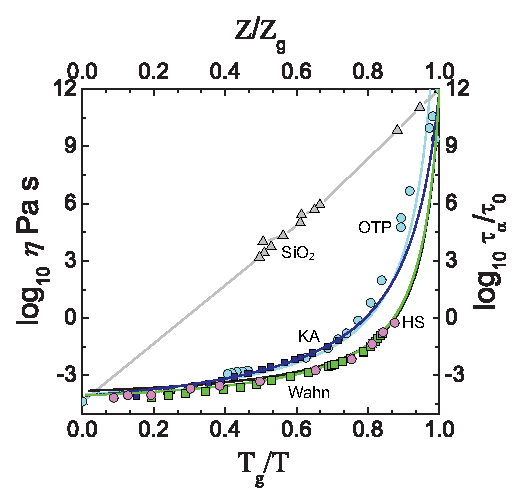
\includegraphics[width=0.9\linewidth,outer]{angell}
  \caption[The Angell plot for model systems undergoing dynamical arrest]{
    The \emph{Angell} plot \cite{AngellJNS1988} for molecular and model glassformers showing the temperature/pressure dependence of viscosity (labelled here as $\eta$) or equivalently relaxation time $\tau_\alpha$.
    The molecular systems \ce{SiO2} and orthoterphenyl (OTP) respectively display the \emph{strong} and \emph{fragile} behaviours described in text, with data obtained from Refs.\ \cite{AngellS1995, BerthierPRE2009}.
    Kob-Anderson (KA) and Wahnstrom (Wahn) are binary mixtures of Lennard-Jones atoms designed to exhibit fragility.
    The compressibility $Z = \beta p / \rho$ is argued to be equivalent to inverse temperature for hard spheres (HS) \cite{BerthierPRE2009}, with data taken from Ref.\ \cite{RoyallJSM2017}.
    Reproduced from Ref.\ \cite{RoyallPR2015}.
  }
  \label{fig:angell}
\end{SCfigure}

Our focus is on soft matter, with hard spheres as the prototypical model, where the  interactions (typically van der Waals attractions) are much weaker than in molecular systems (and absent in hard spheres).
Consequently, there is less of a case for an Arrhenius relationship \eqref{eq:arrhenius-law}, and empirically we find striking deviations from it.
Many systems show \emph{super-Arrhenius} scaling with temperature (Fig.\ \ref{fig:angell}), including mixtures of Lennard-Jones atoms and molecular systems such as orthoterphenyl.
Correspondingly, systems where $\tau_\alpha$ increases more rapidly than exponential are labelled as \emph{fragile}.
A super-Arrhenius scaling of $\tau_\alpha$ implies that the thermodynamic barrier to relaxation $\Delta \Phi_\alpha$ increases with supercooling.
This means that the dynamics fundamentally changes at high densities (or low temperatures), which must be caused by the onset of \emph{collective} (or \emph{cooperative}) effects; given the weakness of bonds in soft matter, we can conclude that many particles must contribute to create a large barrier.
We will discuss this more in the next section.

Some modification is required for hard particle systems, where temperature is not a natural control parameter.
As we argued in the introduction, pressure is the only meaningful state variable.
The authors of Ref.\ \cite{BerthierPRE2009} argue that pressure plays a role equivalent to inverse temperature in athermal systems, because of similarities in their limit behaviour.
Alternatively, we could make a free volume argument, where we expect a relaxation event to involve fluctuations of volume $\Delta V$.
In equilibrium, volume fluctuations are created by reversible work $p \Delta V$ so to leading order%
\marginfootnote{The leading order behaviour can be given more justification by invoking the morphometric approach \eqref{eq:fmt-morphometric-2}, or from more general arguments which we will introduce in section \ref{sec:insertion-as-solvation}.}
we then expect
\begin{equation*}
  \tau_\alpha \sim e^{\beta p \Delta V}.
\end{equation*}
Taking $\Delta V$ as the equivalent of an energy barrier, we find the conjugate variable $\beta p$ does indeed play the role of inverse temperature.
It is usual to work with the dimensionless \emph{compressibility factor}, defined by
\begin{equation}
  Z = \frac{\beta p}{\rho},
\end{equation}
in terms of which hard spheres show the same phenomenology as thermal systems (Fig.\ \ref{fig:angell}); we find that hard spheres are comparable in fragility to various binary Lennard-Jones mixtures.
Relaxation barriers in hard spheres are entropic in nature, so perhaps it is easier to see the need for collective effects.
Moreover, the geometrical interpretation in terms of volume fluctuations $\Delta V$ provides an intuitive picture for collective motion: at high densities more particles have to move out of the way to create space for motion.

\begin{SCfigure}
  \includegraphics[width=0.7\linewidth,outer]{dynamic-heterogeneity}
  \caption[Dynamical heterogeneity in binary hard discs]{
    Dynamical heterogeneity in a binary hard disc system with a size ratio of $1:1.4$.
    Particles are coloured according to distance moved over a relaxation time $\tau_\alpha$, with blue having moved the least and red the most.
    Reproduced from Ref.\ \cite{RoyallPR2015}.
  }
  \label{fig:dynamic-heterogeneities}
\end{SCfigure}

Given the rapid increase in dynamical timescales with supercooling, there comes a point where the relaxation time exceeds the observation time so it is impossible to equilibrate the system.
This is the \emph{experimental glass transition}, operationally set as the point where $\tau_\alpha(T = T_g \textrm{ or } \eta = \eta_g) = \SI{100}{\second}$.
In some sense, this threshold defines a subjective limit of a human observer's patience, and so the point $T_g$ (or $\eta_g$) is not strictly a transition.
However, in practice $\tau_\alpha$ is increasing so rapidly by this point that the location of $T_g$ (or $\eta_g$) is insensitive to the choice of observation time \cite{CavagnaPR2009}.

As the final piece of the phenomenology we introduce two more important dynamical features which differentiates the supercooled liquid from normal liquids.
First, the Stokes-Einstein equation, relating diffusion, temperature and viscosity, holds at high temperatures (low densities) but significant deviations are observed at supercooling to low temperatures (high densities) \cite{BerthierRMP2011}.
This finding possibly suggests the existence of multiple competing relaxation mechanisms in the supercooled liquid, which are probed differently by the two measures \cite{EdigerARPC2000}.
Second, the dynamics becomes highly spatially heterogeneous at increased supercooling (Fig.\ \ref{fig:dynamic-heterogeneities}).
Furthermore, simulation studies have revealed that the initial configuration strongly correlates with the locations of mobile events \cite{Widmer-CooperJPCM2005}.
This suggests that the sites of mobility are encoded in the static configuration, which could be interpreted structurally.
%The size of these hetereogeneities is captured by a dynamic lengthscale $\xi_\mathrm{dyn}$, whereas thermodynamic theories typically concern static lengthscales.
%A requirement of a thermodynamic theory is thus that $\xi_\mathrm{dyn}$ scales with the proposed static length.

%% To unveil static quantities, it is tempting to link dynamical heterogeneity to structural heterogeneity.
%% Stable structures should move less than unstable ones.
%% Widmer-Cooper and Harrowell 11 demonstrated that the initial configuration of a simulation, independently of the initial dynamics, has a role in the heterogeneity of the dynamics.

The main point of contention is over what causes this slow-down: whether it is driven by an underlying phase transition in the thermodynamic viewpoint, or if it is purely a kinetic effect.
The former viewpoint includes the related \emph{mode-coupling} and \emph{random first-order transition} theories, which are loosely based on mean-field theory.
By contrast, the kinetic viewpoint \emph{dynamical facilitation} is based entirely around study of fluctuations.
Having introduced the phenomenology of supercooled liquids we can now proceed to discuss these theories in turn.
We will emphasise the thermodynamic theories because in recent years there has been a substantial shift towards them because of the success of mean-field theories.
Furthermore, our approach focuses on static many-body correlation functions and local structure, which lends itself more towards a thermodynamic viewpoint.

%These are not \emph{completely} mutually exclusive viewpoints, as it is possible hybrid scenarios exist where a phase transition is 

%% We discussed the static correlation functions at length, which is fine for liquids where equilibrium occurs on a \SI{100}{\pico\second} timescale.
%% Dynamical effects are highly nontrivial at high densities.
%% As a practical definition, a glass is defined in the lab as any material for which the relaxation time exceeds \SI{100}{\second}: this point is called the experimental glass transition.
%% This is somewhat arbitrary, although the location of the glass transition point is not particularly sensitive to where you set the threshold because of how rapidly the viscosity/times are increasing around there.
%% So what do we mean by dynamical arrest.

%% Cooling a liquid.
%% Take thermodynamic quantity (e.g.\ volume, entropy, enthalpy): usually crystallise.
%% (Picture)
%% First-order transition bypassed by quick cooling.
%% Enter supercooled liquid phase.

%% Both of these conditions are violated in the glass, as this is a truly non-equilibrium state.
%% That is, we see ageing, and hysteresis in response to perturbations.
%% No longer equilibrates/relax/flows, call it a glass: occurs at glass transition.
%% Glass is a solid for all practical purposes.
%% Distinguished from glass which has dependence on preparation history, hysteresis/memory effect of heating the system (will not follow exactly the same curve until - back to the equilibrium supercooled structure), aging: averages (including correlations) evolve in time.

%% The glass transition itself is not a ``transition'' in the thermodynamic sense; there is no.
%% It's really a kind of impatience transition; the glass transition for a human would be different to the glass transition for a demigod/ent.
%% It's still a relatively robust measurement, because of the superarrhenius scaling (sc-l for pedestrians).

%% A plethora of questions related to the out-of-equilibrium properties.
%% \begin{enumerate}
%% \item Properties of out of equilibrium glass phase: very important questions for material science. Low temperature anomalies, aging behaviour, nonlinear rheology  plasticity.
%% \item Relation between glass and jamming. Jamming=zero temperature, out of equilibrium, infinite pressure.
%% \item How to avoid crystallisation.
%% \end{enumerate}

%% We will talk about this metastable branch as if it were in equilibrium.
%% \todo{create link when mention high density swap data}

%% Relationship with viscosity.
%% Flowing/not flowing is captured by viscosity: viscous slowdown same as relaxation slowdown.
%% Slightly different notion.
%% Short times $t \ll \tau$: elastic system, long times $t \gg \tau$: viscosity.
%% Time barrier is relaxation time.
%% Elasticity, viscosity in Newtonian fluids: viscoelastic behaviour (Maxwell)
%% \begin{equation}
%%   \eta = G_\infty \tau_\mathrm{relax}
%% \end{equation}
%% high frequency shear modulus is elastic property.
%% Shear modulus increases by factor 2-5 times, is dwarfed by change in relaxation time.

\section{Mode-coupling theory}
\label{sec:mct}

The central tenet of mode-coupling theory (MCT) is to separate the liquid's degrees of freedoms into \emph{slow} and \emph{fast} variables.
Fast variables are those that thermalise very quickly, e.g.\ the solvent in a colloidal liquid, so that they can be integrated out leaving only slowly evolving variables of interest.
We advocate essentially the same philosophy, of coarse-graining onto a few dynamically relevant degrees of freedom, in developing a theory for many-body correlations in chapters \ref{chapter:morphometric-framework} and \ref{chapter:morphometric-applications}.
The difference between the two approaches is that MCT explicitly treats \emph{dynamical} processes whereas we focus on \emph{static} correlations.
We will discuss our own approach more in section \ref{sec:correlation-perspective}.

As an example of separation into fast and slow variables, consider classical Langevin equation of motion.
%, which expresses the equations of motion of a subset of the degrees of freedom.
Newton's equation for a particle in an external field becomes
\begin{equation}\label{eq:classical-langevin}
  m \ddot{\vec{r}}
  =
  \vec{\nabla} \phi_\mathrm{ext}(\vec{r})
  - \lambda \dot{\vec{r}} + \vec{f}(t)
\end{equation}
where $m$ is the particle mass, $\lambda$ is a coefficient of damping and $\vec{f}$ is the \emph{fluctuating force} from the fast variables, normally approximated as a Gaussian random field
\begin{equation*}
  \langle f_i(t) f_j(t') \rangle = 2 D \delta_{i,j} \delta(t - t'),
\end{equation*}
with diffusion constant $D$.
Here, the position $\vec{r}$ represents the slowly evolving variable of interest, whereas the remaining degrees of freedom (e.g.\ small solvent particles) are imagined to equilibrate rapidly leaving only the force field $\vec{f}$.

Mode-coupling theory starts from a formally \emph{exact} Langevin equation, which generalises the classical result \eqref{eq:classical-langevin} above.
Defining the instantaneous state of the liquid as
\begin{equation*}
  \vec{X}(t) := \begin{pmatrix} \hat\rho(\vec{r}, t) \\ \vec{\hat{j}}(\vec{r}, t) \end{pmatrix}
\end{equation*}
with instantaneous current $\vec{\hat{j}}(\vec{r}, t) := \partial \hat\rho(\vec{r}, t) / \partial t$, the generalised Langevin equation then reads \cite{ReichmanJSM2005, JanssenFP2018}
\begin{equation}\label{eq:general-langevin}
  \frac{d \vec{\widetilde{X}}(\vec{k}, t)}{dt}
  =
  i \vec{\Omega} \cdot \vec{\widetilde{X}}(\vec{k}, t)
  - \int_0^t \vec{K}(t') \cdot \vec{\widetilde{X}}(\vec{k}, t - t') \, dt'
  + \vec{f}(t)
\end{equation}
where $\vec{f}$ is (again) the fluctuating force obtained by integrating out the fast degrees of freedom, $\vec{K}(t')$ is a time-dependent \emph{memory function} containing the history of $\vec{f}$ as an autocorrelation function \cite{ReichmanJSM2005} and $\vec{\Omega}$ is the \emph{frequency matrix} containing the forces internal to the slow variables \cite{JanssenFP2018}.
Each of these terms has an allegory in the classical Langevin equation \eqref{eq:classical-langevin} above.
Similar equations to \eqref{eq:general-langevin} can be constructed for observables such as the correlation functions; the goal of MCT is to construct (and solve) an equation for $F(\vec{k}, t)$ \eqref{eq:isf} obtaining the dynamical behaviour of the liquid at long times.
The central challenge of this approach is finding suitable approximations for the memory function $\vec{K}$.
%% \begin{equation*}
%%   \vec{K}(t') = \vec{f}(0)^T \vec{f}(t') \cdot (\vec{\widetilde{X}}^T \vec{\widetilde{X}})^{-1}.
%% \end{equation*}

In the standard MCT approach, the fluctuating force is assumed to be dominated by the pair correlations so that $K$ becomes a four-point correlation function.
Then, through a second approximation where $K$ is factorised into a product of two two-point correlation functions, it is possible to construct an evolution equation for the intermediate scattering function \eqref{eq:isf} as \cite{ReichmanJSM2005}
\begin{equation}\label{eq:full-mct}
  \frac{d^2 F(k,t)}{d t^2}
  + \frac{k^2}{\beta m S^{(2)}(k)} F(k, t)
  + \int_0^t K_\mathrm{MCT}(k, t') \frac{d F(k, t - t')}{dt} \, dt'
  =
  0
\end{equation}
with
\begin{subequations}\label{eq:full-mct-coupled}
  \begin{align}
    K_\mathrm{MCT}
    &=
    \frac{\rho}{16 \pi^3 \beta m}
    \int |V_{\vec{q},\vec{k}-\vec{q}}|^2
    F(q, t) F(|\vec{k} - \vec{q}|, t)
    \, d\vec{q},
    \\
    V_{\vec{q},\vec{k}-\vec{q}}
    &=
    \frac{
      \vec{k} \cdot \vec{q} c^{(2)}(q) + \vec{k} \cdot (\vec{k} - \vec{q}) c^{(2)}(|\vec{k} - \vec{q}|)
    }{
      k
    }.
  \end{align}
\end{subequations}
The latter function $V_{\vec{q},\vec{k}-\vec{q}}$ is the so-called \emph{vertex}, which takes the pair direct correlation, and the initial condition for \eqref{eq:full-mct} is $F(k,t=0) = S^{(2)}(k)$; as such, standard MCT takes only pair correlation functions as input.
Together \eqref{eq:full-mct} and \eqref{eq:full-mct-coupled} form a non-linear coupled set of integro-differential equations that can be numerically solved, providing a reasonable description of the \emph{onset} of dynamical arrest, with deviations only becoming noticeable at deep supercooling \cite{FlennerPRE2011,BrambillaPRL2009}.

Crucially, MCT predicts a diverging timescale at $\eta \sim 0.52$ in hard spheres, where the dynamics would become completely arrested, and numerical fits to colloidal experimental data with the same power behaviour law predicted by MCT move this point up to $\eta \sim 0.58$ \cite{VanMegenPRE1994}.
However, this predicted transition must be spurious as recent experiments have managed to equilibrate colloidal hard sphere liquids up to $\eta \lesssim 0.60$ \cite{BrambillaPRL2009,HallettNC2018} and to even higher densities in simulations \cite{BerthierPRL2016}.
Despite this failing of MCT, it remains the only properly first-principles theory for treating liquid dynamics.

Extensions incorporating fluctuations can be found in Refs.\ \cite{BiroliPRL2006,SzamelPTEP2013}, and more recently a generalised MCT has been developed which avoids the uncontrolled factorisation of the pair densities \cite{JanssenPRL2015,JanssenFP2018}.
Importantly, the latter approach incorporates closures of the many-body correlation functions, which will be a central theme of later chapters; by doing this the authors were able to move the diverging timescale to higher densities, bringing the theory into better agreement with available data from simulations and experiments.

\section{Mean-field theories}
\label{sec:mean-field-glass}

We introduced MCT as an explicitly dynamical theory which attempts to model dynamical arrest in supercooled liquids by directly describing the decay of time correlation functions like $F(k, t)$.
Thermodynamics only entered implicitly into MCT through the structural input of the static structure factor $S^{(2)}(k)$.
By contrast, \emph{mean-field theories} of glass take a primarily thermodynamic approach, though they are broadly compatible with the dynamical descriptions of MCT.
The mean-field picture has been rapidly gaining traction in recent years since exact solutions have been developed for hard spheres \cite{ParisiRMP2010,KurchanJSM2012,KurchanJPCB2013,CharbonneauNC2014,CharbonneauJSM2014}.
To describe mean-field theory we will invoke the concept of an \emph{energy landscape}, the natural generalisation of transition state theory introduced in section \ref{sec:glass-phenomenology} and summarised by \eqref{eq:reaction-time}.
While this conceptual framework is not unique to mean-field theories, it is most closely associated with them.

In an energy landscape description, the thermodynamic potential is interpreted \emph{geometrically} as a mapping from every point in configuration space to a `height' representing energy e.g.\ $\Phi: \mathbb{R}^{dN} \mapsto \mathbb{R}$ for an $N$ particle system.
The appeal of this approach is that physical processes can be understood \emph{topographically}: the system will spend more time at the bottom of `valleys' (minima of $\Phi$), especially at lower temperatures, and dynamics will occur primarily through low-lying `mountain passes' (saddles of $\Phi$) \cite{StillingerS1995}.
The timescales of transitions over saddles are expected to scale via the usual Boltzmann weight \eqref{eq:reaction-time}, just as in ordinary transition state theory, however this refined picture emphasises the importance of landscape \emph{connectivity}: the number, separation and relative weights of the various dynamical paths could drive the glass transition.

The energy landscape is particularly relevant in mean-field, formally corresponding to the high dimensional limit%
\marginfootnote{To understand why, consider the typical number of particle neighbours increases with dimensionality.
  Then, formally in the limit $d \to \infty$ a particle is able to achieve a macroscopic number of neighbours, equivalent to an interaction with an average field representing the rest of the system.}
$d \to \infty$, because its \emph{exact} properties can be determined.
In mean-field, hard spheres undergo a \emph{clustering} (or \emph{dynamical}) transition at a volume fraction $\eta_c$ where the landscape splits into disconnected regions \cite{ParisiRMP2010,KurchanJSM2012,KurchanJSM2016}, and the dynamics are described by an almost identical theory to MCT \cite{MaimbourgPRL2016,KurchanJSM2016}.
As configuration space becomes disconnected at $\eta_c$, the system is frozen into a single region and so the relaxation time diverges; contemporaneously, the memory function analogous to $K_\mathrm{MCT}$ in mean-field develops a plateau reflecting the fact that the density profile can no longer completely relax \cite{CharbonneauARCMP2017}.
In this light, the diverging relaxation time predicted by standard MCT is not necessarily a failure of the theory, but is indicative of this genuine mean-field transition.

Although the dynamics is singular at the dynamical transition, the thermodynamic observables are continuous as the system is compressed beyond $\eta_c$ \cite{ParisiRMP2010}.
%% Starting from the definition of the Helmholtz free energy.
%% \begin{equation*}
%%   F = \langle U \rangle - T S.
%% \end{equation*}
We can imagine what happens to the system under further compression if it could continue to sample these disconnected regions in equilibrium, i.e.\ with Boltzmann weighted measure.
The free energy, normally expressed as a sum over all microstates%
\marginfootnote{Which microstates this includes depends on the ensemble.}
$\Gamma$, can be re-expressed as a sum over a collection of \emph{mesostates} $\Gamma = \{\alpha_1, \cdots, \alpha_M\}$ giving
\begin{equation}
%\begin{subequations}
  %\begin{align}
    \Phi = \sum_{i \in \Gamma} p_i \, (\epsilon_i - k_B T \, \ln{p_i})
   % \\
    = \overline{\Phi} - T \Sigma
  %\end{align}
%\end{subequations}
\end{equation}
where $\epsilon_i$ is the energy of microstate $i$ and $p_i$ its probability measure.
In the latter step we defined%
\marginfootnote{This expression is obtained by writing the probability of the system being in mesostate $\alpha$ as $p_\alpha = \sum_{i \in \alpha} p_i$, then $p_i / p_\alpha$ is the probability of microstate $i$ given that the system is in this mesostate.}
\begin{subequations}
  \begin{align}
    \overline{\Phi}
    &=
    \sum_\alpha p_\alpha
    \underbrace{
      \sum_{i \in \alpha} \frac{p_i}{p_\alpha}
      \left(
      \epsilon_i - k_B T \, \ln{\frac{p_i}{p_\alpha}}
      \right)
    }_\textrm{free energy of mesostate $\alpha$},
    \\
    \Sigma &= - k_B \, \sum_\alpha p_\alpha \ln{p_\alpha}.
  \end{align}
\end{subequations}
The \emph{complexity} $\Sigma$ is an extensive quantity characterising the multiplicity of mesostates; at the dynamical transition this becomes a positive non-zero number $\Sigma(\eta = \eta_c) > 0$ corresponding to the clustering in configuration space.
As the system is compressed further $\Sigma$ decreases \cite{KirkpatrickPRB1987,KirkpatrickPRA1989,ParisiRMP2010} corresponding to the rarefaction of clustered regions.
At a volume fraction $\eta_K > \eta_c$ an \emph{entropy crisis} occurs: $\Sigma$ vanishes, leading to the system being frozen into a single, unique region in configuration space called an \emph{ideal glass} phase \cite{KauzmannCR1948,KirkpatrickPRB1987,HallJCP1987,KirkpatrickPRA1989,ParisiRMP2010,BerthierRMP2011}.

If an equilibrium glass state in the regime $\eta \in [\eta_c, \eta_K]$ is compressed out-of-equilibrium without sampling the other clusters, a further phase transition occurs to a so-called \emph{Gardner} phase \cite{KurchanJPCB2013,CharbonneauNC2014,CharbonneauJSM2014}.
Each cluster splits further into fractal sub-regions arranged hierarchically.
Whereas the clustered regions formed at $\eta_c$ are geometrically dissimilar%
\marginfootnote{As measured by e.g.\ the intermediate scattering function},
these regions are close in configuration space to one another.
This phase has deep connections with the jamming transition seen at diverging pressure, providing a unified description of glass and jamming conjectured since the landmark paper of Ref.\ \cite{LiuN1998}.
Remarkably, this mean-field theory is able to predict anomalous $d$-independent critical scaling coefficients, matching those known around jamming \cite{WyartPRL2012,LernerSM2013,DeGiuliPNAS2014}.
The existence of the Gardner phase provides context for the importance of mean-field theory, but it cannot be directly connected to our approach in subsequent chapters so we will not discuss it further.
For more information on the mean-field Gardner phase see the reviews of Refs. \cite{BerthierJCP2019,CharbonneauARCMP2017}.

%% Specifically, the glass transition can be understood as the division of the energy landscape up into subunits??
%% Exact properties of the energy landscape can be determined for many mean-field systems, where it is known to play a leading role in dynamical arrest.

The mean-field picture introduces complexity as the important quantity of interest, relating the number of metastable regions in configuration space.
The relevance of mean-field descriptions in physical dimensions requires a finite-dimensional description of the supercooled liquid and its energy landscape.

%% In physical dimensions, the energy landscape does not become completely disconnected, so transitions between metastable states are possible; the dynamical transition becomes a cross-over.
%% As such, a finite-dimensional description of the supercooled liquid is needed.

%% In physical dimensions, the energy landscape does not become
%% This quantity is well-defined in mean-field because these regions are completely disconnected, however in finite dimensions transitions can always occur between them through nucleation \cite{KirkpatrickPRB1987,KirkpatrickPRA1989,BouchaudJCP2004}.
%% The dynamical transition thus becomes a cross-over, and a finite-dimensional description of the supercooled liquid is needed.

\section{Finite-dimensional theories}
\label{sec:finite-d-glass}

\begin{SCfigure}
  \includegraphics[width=0.9\linewidth,outer]{swap-Sconf}
  \caption[Configurational entropy in hard spheres from Monte-Carlo simulations]{
    Configurational entropy in hard spheres from novel Monte-Carlo (MC) simulations for a system with 23\% polydispersity.
    $Z_0 \approx 18$ ($\eta_0 \approx 0.56$) marks the onset pressure, above which the intermediate scattering function $F(k,t)$ decays non-exponentially, and $Z_c \approx 23.5$ ($\eta_c \approx 0.598$) is the location of the dynamical transition predicted by fitting mode-coupling theory's power-law scaling to the lower density behaviour.
    The various methods used (described in Ref.\ \cite{BerthierPNAS2017}) all broadly agree that this quantity is trending to zero at a finite pressure, suggesting the existence of a thermodynamic glass transition.
    The equation of state for this system is given in Fig.\ \ref{fig:swap-eos}.
    Reproduced from Ref.\ \cite{BerthierPNAS2017}.
  }
  \label{fig:swap-sconf}
\end{SCfigure}

%% Mean-field theories have traditionally been formulated in configuration space, in terms of the energy landscape.
%% By contast, in $d=3$ the existence of dynamical heterogeneity calls for a real space interpretation.

The relevance of mean-field ideas in physical dimensions can be seen by an interpretation of Refs.\ \cite{KirkpatrickPRB1987,HallJCP1987,KirkpatrickPRA1989}, with antecedent ideas found in \cite{KauzmannCR1948,AdamJCP1965}.
This \emph{random first-order transition} (RFOT) scenario acknowledges that the clustering of states appearing at the dynamical transition in mean-field will not be strictly metastable over finite lengthscales in finite $d$ \cite{BouchaudJCP2004,MontanariJSP2006}.
As such, the complexity is not well-defined because the metastable states will not be strictly separated with infinite barriers, though they may be arbitrarily long-lived; the dynamical transition of mean-field thus becomes a cross-over.
In finite dimensions, the \emph{configurational entropy} $S_\mathrm{conf}$ is introduced as the closest equivalent to the complexity; this does not have a generally agreed upon meaning, but a common definition invokes the timescale separation between vibrational ($\beta$--) and liquid-like ($\alpha$--) dynamics.
The configurational entropy then describes the entropy of the latter process, obtained as the residual entropy after removing vibrations
\begin{equation}\label{eq:sconf}
  S_\mathrm{conf} := S - S_\mathrm{vib},
\end{equation}
though some refinement is required for polydisperse systems \cite{OzawaJCP2017,OzawaJCP2018} and where additional non-vibrational processes exist that do not relax the density profile \cite{OzawaPRL2018}.

The RFOT scenario imagines the mean-field dynamical transition as a crossover to an \emph{energy landscape dominated} dynamics.
Specifically, the number of unique (non-vibrational) states possible in a subregion of size $\xi$ will scale $\propto \exp{(s_\mathrm{conf} \xi^d / k_B)}$, where $s_\mathrm{conf} = S_\mathrm{conf} / V$ is the configurational entropy density.
A dynamical event which changes a state is expected to pay an energy penalty $\gamma_\mathrm{eff} \xi^\theta$ where $\theta \le d$ from inducing a mismatch with the surrounding fluid.
The thermodynamic potential for this subregion is then expected to adopt the form
\begin{equation}\label{eq:rfot-barrier}
  \Phi \sim \gamma_\mathrm{eff} \xi^\theta - T s_\mathrm{conf} \, \xi^d.
\end{equation}
The maximum of $\Phi$ occurs at the \emph{point-to-set}%
\marginfootnote{So-named because this lengthscale marks the crossover from the subregion being confined to a single `point' in its configuration space to a `set' of states.}
length
\begin{equation}\label{eq:rfot-xi}
  \xi_\mathrm{PS}
  := \argmax{(\Phi)}
  \sim
  \left(
  \frac{\theta \gamma_\mathrm{eff}}{d T s_\mathrm{conf}}
  \right)^\frac{1}{d-\theta},
\end{equation}
after which $\Phi$ grows infinitely negative, so the metastable states are unstable to activated dynamics for $\xi \gtrsim \xi_\mathrm{PS}$.
The RFOT interpretation thus predicts the formation of a \emph{mosaic} of droplets of typical lengthscale $\xi_\mathrm{PS}$ \cite{KirkpatrickPRB1987,HallJCP1987,KirkpatrickPRA1989,BouchaudJCP2004}.
The nature of the entropic droplets forming the mosaic state and the processes by which they relax is an active area of study \cite{BouchaudJCP2004,DzeroPRB2005,FranzJSM2005,AngeliniJSP2017,RulquinJSM2016,BiroliMeanPRB2018,BiroliFinitePRB2018}.
Notably, a lot of attention has been devoted to the treatment of the subleading term $\gamma_\mathrm{eff} \xi^\theta$.

This thermodynamic argument above concerns whether a region of the liquid \emph{will} relax eventually, but an even more direct connection with relaxation timescale was proven in Ref.\ \cite{MontanariJSP2006}.
Briefly, dynamical barriers must remain finite within a finite subregion, so they scale Arrheniusly via \eqref{eq:reaction-time}; any Arrhenius process will eventually overwhelm the super-Arrhenius scaling of $\tau_\alpha$ at deep supercooling.
Fragile behaviour then suggests a reduction in $S_\mathrm{conf}$ to limit the number of possible Arrhenius processes.
Moreover, the authors of Ref.\ \cite{MontanariJSP2006} then show that the relaxation time is rigorously bounded from above by $S_\mathrm{conf}$, proving that any diverging relaxation time \emph{must} coincide with an entropy crisis where $S_\mathrm{conf}$ becomes sub-extensive.
Measurements of the configurational entropy from simulations of hard spheres suggest a vanishing $S_\mathrm{conf}$ at finite pressure in $d=3$ (Fig.\ \ref{fig:swap-sconf}), pointing to a mean-field/RFOT scenario in hard spheres.
However, this necessarily relies on extrapolation as the point where $S_\mathrm{conf}$ vanishes cannot be reached in finite time because of the argument above.

%% Mean-field argument is thermodynamic, which in some sense is structural.
%% Structural in the sense of the energy landscape, not necessarily in real space/local structure.
%% The real space interpretation of mean-field theory is random first-order transition theory (RFOT), also called \emph{mosaic} theory.

%% In conventional condensed matter physics dynamics is determined by structure.
%% For example, crystalline solids are fixed on a lattice so do not flow, whereas liquids are disordered and are thus able to flow.
%% Soft matter systems (e.g.\ gels, foams, glasses) do not neatly fall into this paradigm: their dynamics are often arrested whilst their structure remains highly disordered.

\begin{SCfigure}
  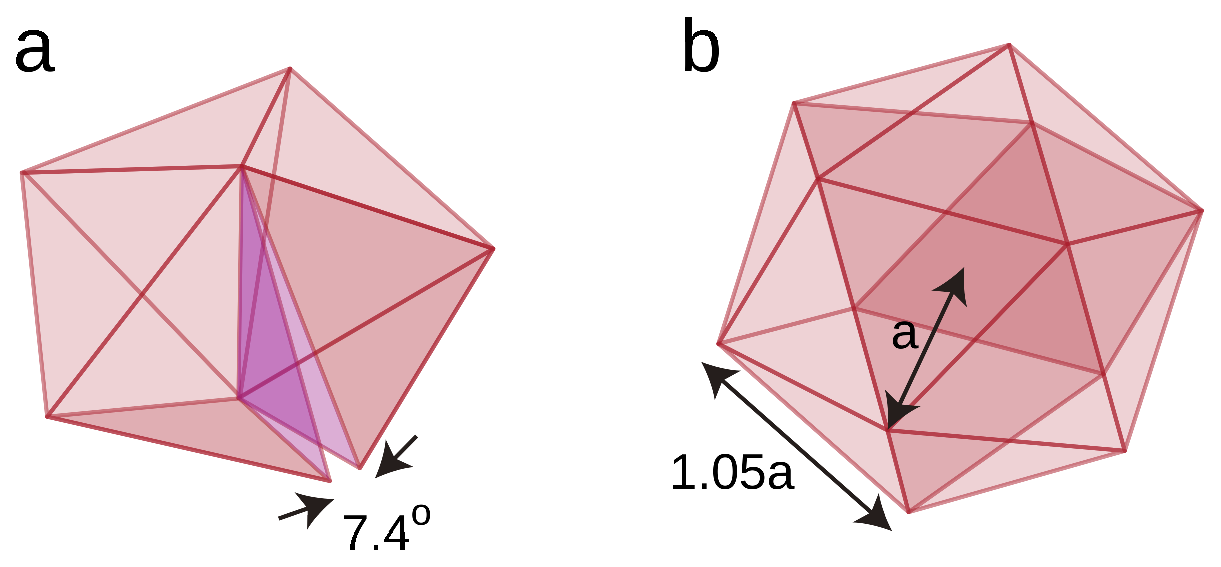
\includegraphics[width=0.7\linewidth,outer]{frustration}
  \caption[Frustration of tetrahedral structures]{
    Structures formed by combining tetrahedra.
    (a) The pentagonal bipyramid constructed from five regular tetrahedra must leave a small gap of \SI{7.4}{\degree}.
    (b) The icosahedron formed by vertices a distance $a$ from the centroid must have edge length $\sim1.05 a$, so if hard spheres of diameter $a$ were placed on the vertices they would not be in contact.
    Reproduced from Ref.\ \cite{RoyallPR2015}.
  }
  \label{fig:frustration}
\end{SCfigure}

A different scenario in physical dimensions focuses on the role of geometry.
This picture starts from the observation that crystal structures (e.g.\ the face-centred cubic introduced for hard spheres at close packing) are generally not the optimal energetic arrangement for small clusters of particles, even though they must be for bulk systems.
For example, 13 isolated Lennard-Jones atoms will preferentially arrange as vertices of a fivefold symmetric \emph{icosahedron} \cite{FrankPRS1952} (Fig.\ \ref{fig:frustration}b).
As fivefold symmetric structures cannot tessellate Euclidean space, Sir Charles Frank conjectured that glassformers suppress crystallisation through formation of icosahedra (or similar structures) \cite{FrankPRS1952}.

The above viewpoint has been developed into the more complete theory called \emph{geometric frustration} \cite{KivelsonPA1995,TarjusJPCM2005}.
This approach characterises the liquid by its \emph{locally favoured structures} (LFS), i.e.\ those structures which are energetically favoured at small length scales.
A system could have a single LFS, or a whole collection; recently, it has been shown through numerical simulations that \emph{competition} between different LFS enhances the propensity for glassformation \cite{TeichNC2019}.
This competition is an example of \emph{frustration} where continual growth of domains of LFS is hindered by geometric constraints.
Frustration can also emerge from a single LFS if it cannot tile space, as is the case of fivefold symmetric structures like icosahedra.
Incorporating frustration into a theory modelling the energy of LFS-rich domains leads to a similar scaling relation as in RFOT \eqref{eq:rfot-barrier}, though the resulting phase behaviour is quite different.
The static lengthscale which emerges from this theory is interpreted as the size of the domains, which is more easily understood than the amorphous lengthscale $\xi_\mathrm{PS}$ of RFOT.
Details can be found in the review of Ref.\ \cite{TarjusJPCM2005}.

The frustration picture is broadly compatible with the mean-field viewpoint: the propensity for a system to form certain structures can be interpreted as a manifestation (or a driving force) of a reduced $S_\mathrm{conf}$.
The downside of this scenario is that the correlation between local structure and dynamics seems to be highly system dependent \cite{HockyPRL2014}.

Whereas RFOT postulates amorphous order, geometric ideas propose simpler static orderings based around e.g.\ LFS domains.

CPR: local structure fixes gel \cite{RoyallNM2008}.
Charbonneau: growth of length scale associated with LFS does not correlate with dynamical length scale \cite{CharbonneauPRL2012}, possibly multiple relaxation mechanisms or a non-static length scale.
Leacmach: \cite{LeocmachNC2012}
Coslovich: \cite{CoslovichJCP2007,CoslovichJCP2007a}
Turci: \cite{TurciPRL2017}

In hard spheres, the dominant LFS are found to be icosahedral motifs in accordance with Frank's original conjecture.
In Fig.\ \ref{fig:icosahedral-domains} we see the growth of large domains of icosahedra in the supercooled liquid, over a range in densities where $\tau_\alpha$ changes by a factor of $\mathcal{O}(10^5)$ (Fig.\ \ref{fig:g2-changes}) \cite{HallettNC2018}.
This fact demonstrates that significant structural change occurs alongside dynamical arrest, even though minimal changes are seen at the pair level.
This does not prove that structural change \emph{causes} the slowdown, but it does suggest the idea is worth investigating.
%Furthermore, the vicinity of an icosahedral motif is found to be highly correlated with local particle mobility \cite{HallettNC2018}.

%At high densities the tetrahedra form large connected domains \cite{HallettNC2018} rich in fivefold symmetric structures.
Spherical packings ideally form regular tetrahedra which cannot perfectly form pentagonal structures (Fig.\ \ref{fig:frustration}), so fivefold symmetric structures are highly frustrated.
A detailed review on the role of local structure in glassy systems can be found in Ref.\ \cite{RoyallPR2015}.
\todo{Should definitely cite more Royall group work here, possibly Tanaka too. What's the most appropriate cross-section of papers?}

%% The mean-field picture of glass formation interprets the dynamical slowdown entirely within a thermodynamic framework.
%% In mean-field hard spheres, formally in the limit of infinite spatial dimensions $d \to \infty$,
%% Hard spheres in mean field have been shown to have a thermodynamic glass transition, however the critical dimensions are unknown so it is unclear what happens in $d=3$. \cite{ParisiRMP2010,KurchanJSM2012,KurchanJPCB2013,CharbonneauNC2014,CharbonneauJSM2014}.
Recent numerical evidence suggests that $S_\mathrm{conf}$ only vanishes at $T=\SI{0}{\kelvin}$ for a model glassformer in $d=2$ \cite{BerthierNC2019}.
As this point cannot be crossed no thermodynamic transition can occur in $d = 2$, pointing to a lower critical dimension for mean-field theory of at least $d_L \ge 2$.
It is possible that low-dimensional fluctuations prevent any thermodynamic transition, and it has been argued that even if there is a thermodynamic transition at $\eta_K$ this may not be responsible for the dynamic slowdown seen around the operational glass transition $\eta_g \ll \eta_K$ \cite{WyartPRL2017}.
As such, there is room for alternative pictures to the mean-field/RFOT scenario.

The main opposition theory is \emph{dynamic facilitation}, which focuses on the dynamic heterogeneities as the fundamental feature of glass.
In this picture dynamical events occur through string-like motion between dynamical defects, and the relaxation time remains finite until $T = \SI{0}{\kelvin}$.
\todo{Paddy: Expand on this substantially}
For more information on dynamic facilitation we direct the reader to the review of Ref.\ \cite{ChandlerARPC2010}.
%This must trivially occur at the very least $T=0\si{K}$ where relaxation timescales diverges, however much like the lack of a phase transition in the Ising model in $d=1$ this is not a true thermodynamic phase transition because it cannot be crossed.
%So the central question of glass is what happens in $d=3$, is there a vanishing configurational entropy at a finite $T > 0$ with an accompanying thermodynamic glass transition?

%Theories concentrating on the high density glass: elastic theories.

\begin{SCfigure}
  \includegraphics[width=\linewidth,outer]{icosahedra-hallett}
  \caption[Growth of icosahedral domains in the supercooled hard sphere liquid]{
    Growth of icosahedral domains in a colloidal hard sphere liquid with supercooling, i.e.\ increased volume fraction $\eta$, over a density change which coincides with minimal structural change at the pair level (Fig.\ \ref{fig:g2-changes}).
    (a) STED nanoscopy image for $\eta = 0.598$, with scale bar \SI{3}{\micro\meter}.
    (b), (c) Rendered coordinates of partial icosahedra (green, top right structure) and full icosahedra (purple, bottom right structure) for volume fractions (b) $\eta = 0.523$ and (c) $\eta = 0.598$.
    Reproduced from Ref.\ \cite{HallettNC2018}.
  }
  \label{fig:icosahedral-domains}
\end{SCfigure}

\section{Perspective: usefulness of many-body correlations}
\label{sec:correlation-perspective}

In subsequent chapters will be heavily focusing on the treatment of static many-body correlation functions in the bulk liquid.
Here, we motivate their study for the treatment of the supercooled liquid.
It is natural to wonder what new information can be obtained from the many-body correlation functions that is not already present at the pair level.
In section \ref{sec:thermodynamic-routes} we saw how the compressibility and virial routes lead to expressions of the free energy in terms of pair correlations.
This is emblematic of conventional routes to the free energy, so in some sense all of the thermodynamically relevant information is contained in the two body correlation functions.

Firstly, while it is true that thermodynamic quantities like the pressure can certainly be inferred from the pair correlations, there is no such simple relationship for dynamical quantities.
In the absence of a thermodynamic phase transition, we would not expect the pair correlation function alone to reveal much about the nature of dynamical arrest, beyond the lack of a transition.
Even supposing the existence of a transition, the precision required to detect such a signal $g^{(2)}(r)$ may be arbitrarily subtle; however, any changes approaching a transition \emph{must} be magnified at the many-body level because of \eqref{eq:correlation-derivatives}.
The many-body correlation functions have potential to place the entropic droplet scenario of \eqref{eq:rfot-barrier} on more rigorous footing, by providing a means to calculate the subleading penalty term $\gamma_\mathrm{eff} \xi^\theta$.
Alternatively, the theories which postulate local mechanisms such as the LFS in geometrical viewpoints or the dynamical defects in facilitation should be identifiable within the many-body correlation functions.

Secondly, even at the thermodynamic level the many-body correlations have advantages.
To illustrate this we borrow an argument originally made by Evans \cite{EvansPrivate2019}.
Pair correlations yield thermodynamic quantities which are \emph{derivatives} of the free energy at an instantaneous state point, so to infer the free energy multiple state points must be sampled.
Equivalently, we could consider the derivatives of the pair correlation function.
It is straightforward to show that \cite{Santos2016}
\begin{equation}\label{eq:correlation-derivatives}
  \chi_T \rho
  \left( \frac{\partial \rho^{(n)}}{\partial \rho} \right)_{V,T}
  =
  (n - \rho V) \rho^{(n)}(\vec{r}^n)
  + \int \rho^{(n+1)}(\vec{r}^{n+1}) \, d\vec{r}_{n+1}.
\end{equation}
The important feature to take away from this expression is the presence of $\rho^{(n+1)}$; we see the emergence of higher-order correlation functions in the derivatives.
This means we could in principle measure the free energy at a single state point by introducing highly accurate measurements of the many-body correlation functions.
This is essentially the spirit of the \emph{entropy route}, which writes \cite{WallaceJCP1987}
\begin{equation}
  S = \sum_{n=1}^\infty S_n
\end{equation}
with entropic terms $S_n$ containing contributions from $n$-particle correlations.
The first few terms are given by \cite{WallaceJCP1987}
\begin{subequations}
  \begin{align}
    \frac{S_1}{V}%\langle N \rangle}
    &=
    k_B \, \rho \left( \frac{d}{2} - \ln{\rho \Lambda^d} \right),
    \\
    \frac{S_2}{V}%\langle N \rangle}
    &=
    \frac{\rho^2}{2 T}
    \int g^{(2)}(\vec{r}) \ln{g^{(2)}(\vec{r})}
    \, d\vec{r},
    \\
    \frac{S_3}{V}%\langle N \rangle}
    &=
    \frac{\rho^3}{6 T}
    %\int g^{(3)}(\vec{r}, \vec{r}') \delta w^{(3)}(\vec{r}, \vec{r}')
    \int g^{(3)}(\vec{r}, \vec{r}')
    \ln{\left(
      \frac{
        g^{(3)}(\vec{r}, \vec{r}')
      }{
        g^{(2)}(\vec{r}) g^{(2)}(\vec{r}') g^{(2)}(\vec{r} - \vec{r}')
      }
      \right)}
    \, d\vec{r} d\vec{r}'.
  \end{align}
\end{subequations}
Then, for a pair-interacting system the excess free energy is obtained as
\begin{equation*}
  \begin{split}
    \frac{\beta F^\mathrm{ex}}{V}
    =& \; \hphantom{ + } \;\,
    \frac{\rho^2}{2} \int g^{(2)}(\vec{r})
    \left( \beta u(\vec{r}) - \ln{g^{(2)}(\vec{r})} \right)
    d\vec{r}
    \\ & \;
    + \frac{\rho^3}{6}
    %\int g^{(3)}(\vec{r}, \vec{r}') \delta w^{(3)}(\vec{r}, \vec{r}')
    \int g^{(3)}(\vec{r}, \vec{r}')
    \ln{\left(
      \frac{
        g^{(3)}(\vec{r}, \vec{r}')
      }{
        g^{(2)}(\vec{r}) g^{(2)}(\vec{r}') g^{(2)}(\vec{r} - \vec{r}')
      }
      \right)}
    \, d\vec{r} d\vec{r}'
    \\ & \;
    + \mathcal{O}\left( \rho^4 g^{(4)}(\vec{r}, \vec{r}', \vec{r}'') \right),
  \end{split}
\end{equation*}
so the free energy can be directly obtained from accurate determination of the correlation functions.
%Similarly, a theory treating the many-body correlation functions must have the free energy (and phase behaviour) built in.

We will be focusing on many-body correlations in real space, to explore the local mechanisms proposed in theories of the glass transition described above.
In some situations the correlations in Fourier space may be more useful, most notably in MCT where many-body generalisations have already found some traction \cite{JanssenPRL2015,JanssenFP2018}.
In principle, our real space correlation functions can be Fourier transformed to obtain these, but in practice this is prohibitively expensive because of the high dimensionality of the arguments for even modest values of $n$.
However, FMT already provides an easy route to obtaining all the correlation functions in Fourier space, as described by the original papers \cite{RosenfeldPRL1989,RosenfeldJCP1990}.
We show how to obtain these below.

Fourier transforming the direct correlation functions for the uniform liquid \eqref{eq:fmt-direct-correlations-uniform-density}, and applying the convolution theorem, allows us to write the rather succinct
\begin{equation}
  \widetilde{c}^{(n)}(\vec{k}^n)
  =
  - \sum_{\alpha_1, \alpha_2, \cdots, \alpha_n}
  \partial^n_{\alpha_1, \alpha_2, \cdots, \alpha_n} \beta f^\mathrm{ex} \;
  \left( \prod_{i=1}^n \widetilde{\omega}_{\alpha_i}(\vec{k}_i) \right)
  \delta(\vec{k}_1 + \vec{k}_2 + \cdots + \vec{k}_n).
\end{equation}
The delta function enforces the `ring' condition $\sum_{i=1}^n \vec{k}_i = 0$ which emerges from translational symmetry of the weight functions, reducing the dimensionality of the domain by $d$.
A further $d(d-1)/2$ degrees of freedom%
\marginfootnote{This many degrees of freedom can be removed for general $n \ge d$, but we expect fewer for $n < d$.
  For example, $n=2$ arrangements (a dimer) are isomorphic to a line so they possess $d-1$ rotational degrees of freedom.}
can be removed by exploiting rotational symmetry.
Many-particle generalisations of the static structure factor can be obtained from $\widetilde{c}^{(n)}(\vec{k}^n)$ by functionally differentiating the Ornstein-Zernike equation \eqref{eq:ornstein-zernike-generic} with respect to density \cite{BarratMP1988}.

\section{Summary}

This concludes the relevant background in supercooled liquids and glasses.
In subsequent chapters we will develop a framework for treating the many-body correlation functions in real space, with the hope that it can address some of the questions outlined here.
\todo{More more more, according to Paddy. ``What does it all mean?'' Static lengthscales $=n$}

\ifdefined\includebibliography
  \newgeometry{margin=1in}
  \printbibliography
\fi

\end{document}


\ifdefined\includebibliography
  \printbibliography
\fi

\end{document}

%TC: macro \marginfootnote [other]
%TC: envir SCfigure [] other
%TC: macrocount beginSCfigure [figure]
\documentclass[11pt,twoside]{report}
\usepackage{preamble}
\setcounter{chapter}{2}
\graphicspath{{../img/}}
\def\includebibliography{}

\externaldocument{introduction}
\externaldocument{background}
\externaldocument{morphometric-framework}
\externaldocument{morphometric-applications}
\externaldocument{resummation}
\externaldocument{aerosols}

\begin{document}
\chapter{Supercooled liquids and glasses}
\epigraph{Truly, he thought, the way of enlightenment is like unto half a mile of broken glass.}{Terry Pratchett, \emph{Mort}, (1987).}
\label{chapter:glass}

In the introduction we established the supercooled liquid in hard spheres as the extension of the stable liquid above the freezing density, where it is metastable to the crystal phase.
To provide proper context we will discuss supercooled liquids more generally here, including thermal systems where temperature is the more natural control parameter.
As such, we will be considering the effect of decreasing temperature on the supercooled liquid.

%\hl{This chapter is more of a conventional literature review.}

%% \subsection{Mean-field picture}
%% The infinite dimensional limit $d \to \infty$.

%% \subsection{Random first-order transition theory}
%% Perturbation from mean-field in $1/d$.

%% \subsection{Alternative pictures in physical dimensions}
%% For $d \le 3$
%% \subsubsection{Frustration-limited domain theory}
%% \subsubsection{Dynamical theories}

%% \subsection{Old intro stuff}

%% It is widely reported that glass is actually liquid, and as evidence of this the thickness of old windows at the bottom is pointed to.
%% This is actually a matter of some dispute, but contains a grain of truth.
%% Pre-modern methods of creating window glass involved spinning molten glass on magma to flatten it out.
%% Centrifugal forces caused the glass to be thicker on the outer disc, so panes of glass would always be heavier in one direction%
%% \marginfootnote{And personally, if I were setting an uneven pane of glass I would place the thicker and heavier part at the bottom.}.

%% To a soft matter physicist glass is a broader term, referring to a wide class of materials while the window glass of common parlance is referred to by its chemical name \emph{silicate}.
%% This class of materials share many features of being disordered etc \cite{?} although in some sense they are connected by what they do \emph{not} do: which is flow on human timescales.
%% When I refer to `glass' I will be using it in this broad technical sense of a state of matter.
%% Some examples besides silicate:
%% \begin{itemize}
%% \item Most of the ice in the universe exists in an amorphous state in comets \cite{?}
%% \item Ceramics
%% \item Plastics: amorphous polymers
%% \end{itemize}
%% Of more abstract nature which could be called glassy though they are not materials
%% \begin{itemize}
%% \item Gels: super glasses, liquid like bit plus a network/backbone which has glassy dynamics
%% \item Neural networks
%% \item Non-deterministic polynomial time (NP) problems
%% \end{itemize}
%% We will not be directly addressing the latter type of more abstract problems which could be considered glasses, although they are arguably related due to a similar underlying disorder.
%% We will be focusing on only the most rudimentary of glassy phenomenology: the dynamical arrest of liquids at high densities/low temperatures when crystallisation is avoided.
%% Especially as it manifests in hard spheres, which as discussed is the reference system of choice for simple liquids.

%% Personally, the observation that got me interested in the field is the entropy argument.
%% If one compares the difference between the entropy of the crystal and the glass, and extrapolates wildly one expects there to be a point where the glass has a lower entropy than the crystal.
%% This is not very meaningful by itself, as we have already established by discussing the crystal vibrational entropy can be quite subtle so it is possible for the liquid to have a lower vibrational entropy.
%% However, if one corrects this with more modern techniques to measure just the entropy corresponding to non-trivial motion we see that there is a point where the configurational (i.e.\ not purely vibrational) entropy vanishes: this would imply the system is frozen in a single configuration.
%% Such a point would define a transition to a genuine thermodynamic phase, an ideal glass.

%% Hard glasses: high elastic constants.
%% Colloidal suspensions: soft matter version, small elastic constants.
%% Same phenomenology though.
%% What is a glass?
%% Frozen in a (apparently) disordered state.
%% All sorts of glasses, structural, spin, orientational, electron, vortex.
%% Glasses formed by liquids, colloidal suspensions and polymers: traditional structural glasses.
%% Solid: doesn't flow on observational time, resists small/infinitesimal shear (acts like solid).
%% Amorphous, apparently amorphous: no periodic arrangement like in crystal.
%% Homogeneous makes useful for technology: useful for e.g.\ optical properties.

%First, we describe the phenomenology of supercooled liquids before delving into the specific theories to explain them.

\section{Properties of the supercooled liquid}
\label{sec:glass-phenomenology}

We will start by exploring the ways in which supercooled liquids are the \emph{same} as regular liquids, expanding in more detail on ideas discussed in the introduction.
Then we will move onto the ways in which they \emph{differ} from ordinary liquids, notably in their dynamical properties and their structure at the many-body level.

\begin{SCfigure}
  \includegraphics[width=0.9\linewidth,outer]{g2-evolution}
  %\missingfigure[figwidth=\linewidth]{$g^{(2)}$}%
  \caption[Structural change in the supercooled liquid (at the pair level)]{
    Change occurring in pairwise structure of hard spheres as density is increased above the melting point, as measured by the pair distribution function \eqref{eq:n-particle-distribution}.
    Each state-point is offset for clarity.
    Results for $\eta = 0.45$ were obtained for a 7-component equimolar mixture with 16\% polydispersity using the DynamO software package \cite{BannermanJCC2011}, whereas the data in the metastable regime is from colloidal experiments kindly provided by the authors of Ref.\ \cite{HallettNC2018}.
    The $\alpha$-relaxation times (described in text) in terms of a microscopic time $\tau_0$ are indicated for each state-point, with the last two state-points displaying a large dynamical change with minimal accompanying change in pairwise structure.
  }
  \label{fig:g2-changes}
\end{SCfigure}

Thermodynamically, supercooled liquids are not meaningfully different from their ordinary counterparts.
Operationally, a supercooled liquid is equilibrated in the sense that all observables are time independent and the thermodynamics is self-consistent%
\marginfootnote{Different routes to measuring thermodynamic quantities, e.g.\ the pressure, may give different values in an out-of-equilibrium system.
  This is not the case in supercooled liquids, even though they are not strictly in equilibrium.}.
Formally speaking, the system is sometimes said to be in \emph{local equilibrium}, where it samples all the liquid microstates ergodically; or that it obeys \emph{detailed balance}, where the dynamics is microscopically reversible.
%have very similar structural characteristics as at equilibrium.
As a consequence, the liquid loses any memory of its preparation and all observables become time independent.
That is, for some observable $A$ we can write
\begin{equation*}
  \langle A(t) \rangle = \langle A \rangle.
\end{equation*}
This includes the static correlation functions, introduced in section \ref{sec:liquid-structure}, which remain well-defined in the supercooled regime.
Furthermore, the pair distribution function $g^{(2)}(r)$ changes very little as the density (or temperature) is increased (decreased) from the normal liquid; as an example, we show this for hard spheres in Fig.\ \ref{fig:g2-changes}.
As pair correlations are the main measure of structure in simple liquids, this \emph{seems} to suggest that minimal structural change occurs in the high density liquid.
As a corollary, time correlation functions become \emph{time-translation invariant} meaning they depend only on time differences i.e.\
\begin{equation*}
  \langle A(t) A(t') \rangle = \langle A(0) A(t - t') \rangle.
\end{equation*}
A more sophisticated way in which supercooled liquids can be thought of as equilibrium systems involves the response functions.
In an equilibrium system, the response of a system to a small perturbation is directly related to the microscopic source of fluctuations%
\marginfootnote{Temperature, in the case of liquids.}.
The \emph{fluctuation-dissipation relation} for an observable $A$ expresses the system's susceptibility to a perturbation at time $t'$ as \cite{Chandler1987}
\begin{equation*}
  \chi_A (t, t')
  =
  - \beta \Theta(t - t')
  \frac{d}{dt}
  %\left(
  \big\langle
  \delta A(0)
  \delta A(t - t')
  %% (A(t - t') - \langle A \rangle)
  %% (A(0) - \langle A \rangle)
  \big\rangle
  %\right)
\end{equation*}
where $\delta A(\cdot)$ is the spontaneous and instantaneous fluctuation in $A$, and the Heaviside theta function imposes causality.
These relations are obeyed in supercooled liquids, even though they are not a proper equilibrium state.

In spite of these similarities, supercooled liquids are markedly different from normal liquids in their \emph{dynamics}.
Typically, this is discussed in the context of two (related) quantities: the \emph{viscosity} and the \emph{relaxation time}.
Viscosity measures how resistant the system is to flow, while relaxation time measures the typical microscopic time for the density profile to relax i.e.\ for liquid-like behaviour caused by particle diffusion.
A defining feature of supercooled liquids is that these numbers become so large that the precise details of the measurement used do not matter.
We will discuss this dynamical slowdown further on, but for now we introduce a specific time correlation function in order to frame the discussion.
A popular measurement is the intermediate scattering function, defined by \cite{JanssenFP2018}
\begin{equation}\label{eq:isf}
  F(k, t)
  =
  \frac{
    \big\langle \widetilde{\rho}(\vec{k}, t) \widetilde{\rho}(-\vec{k}, 0) \big\rangle
  }{
    \langle N \rangle
  }
\end{equation}
which reduces to the static structure factor \eqref{eq:static-structure-factor} at zero elapsed time $F(k, t=0) = S^{(2)}(k)$.
An example $F(k,t)$ is shown in Fig.\ \ref{fig:isf}, displaying features which distinguish the supercooled liquid from a regular liquid.
In particular, there is a timescale separation between distinct dynamical processes.
For short times there is a ballistic regime, where particles are essentially free to move unencumbered.
At intermediate times, highly correlated interactions with neighbours inhibit motion and $F(k,t)$ plateaus; this plateau is absent in regular liquids.
Finally, in the long time limit particles are able to diffuse so that $F(k,t)$ completely relaxes to zero.
The latter two processes are called $\beta$- and $\alpha$-relaxation respectively.
The timescale of the longer $\alpha$-relaxation $\tau_\alpha$ is more central to our discussion as it corresponds to the timescale of liquid-like behaviour.

\begin{SCfigure}
  \includegraphics[width=0.9\linewidth,outer]{isf}
  \caption[Intermediate scattering function in a supercooled liquid]{
    Typical intermediate scattering functions in a supercooled liquid.
    In the ordinary liquid decay is purely exponential, but as a liquid is supercooled we observe a timescale separation between short-time vibrational ($\beta$-) and longer time liquid-like ($\alpha$-) relaxation processes.
  }
  \label{fig:isf}
\end{SCfigure}

A helpful framework to guide discussion of dynamical processes is \emph{transition state theory}.
In this approach a dynamical process, e.g.\ a chemical reaction, is imagined to occur through a dynamical bottleneck (Fig.\ \ref{fig:transition-state}).
We imagine evaluating a thermodynamic potential%
\marginfootnote{Which thermodynamic potential this corresponds to will depend on the ensemble.}
$\Phi$ at every point along the reaction path.
The process will then be limited by the rate of thermal fluctuations of size $\Delta \Phi$, i.e.\ those able to reach the transition state.
In equilibrium, the timescale for the process will then scale by the Boltzmann weight
\begin{equation}\label{eq:reaction-time}
  \tau \sim e^{\beta \Delta \Phi}.
\end{equation}
There will be additional kinetic prefactors out in front, however for large barriers we expect the thermodynamic contribution to dominate because of its exponential weighting.
This framework can be more rigorously justified through e.g.\ an \emph{instanton} approach \cite{LangerAP1969}.
The main limitation of transition state theory is the assumption that dynamical processes occur through effectively one-dimensional reaction paths; later, we will introduce a more sophisticated form of this framework which considers the high dimensional \emph{energy landscape}.

As an example of how useful transition state theory can be, we very briefly consider \emph{classical nucleation theory} which we will return to in more detail in chapter \ref{chapter:aerosols}.
Imagining crystallisation to occur by the spontaneous formation of the new phase inside of the liquid, then the timescale for this process will scale as
\begin{equation*}
  \tau_\mathrm{crys} \sim e^{ \beta \Delta \Phi_\mathrm{crys}}.
\end{equation*}
Then, assuming a temperature-independent barrier $\Delta \Phi_\mathrm{crys}$, the timescale for nucleation will increase exponentially as temperature is lowered allowing for the supercooled liquid to become long-lived%
\marginfootnote{Note: the time for crystallisation also scales inversely with system size, so in the thermodynamic limit nucleation occurs instantaneously unless it is strictly forbidden.}
\cite{CavagnaPR2009}.
%This is essentially the reason it is possible for supercooled liquids to exist at all, and reach an effectively time-translation invariant state without decaying to the crystal \cite{CavagnaPR2009}.
This argument is highly system dependent, as systems with small barriers to crystallisation will not be long-lived enough for the metastable liquid to be observed.
Single-component hard spheres are particularly prone to crystallise at very high densities, so polydispersity is typically introduced to frustrate the crystal structure and extend the lifetime of the supercooled liquid.
However, this process is imperfect, as even highly polydisperse systems have been found to crystallise without careful fine tuning of the size distribution \cite{BommineniPRL2019,BerthierPRL2016}.

\begin{SCfigure}
  \includegraphics[width=0.7\linewidth,center]{transition-state}
  \caption[A double-well potential illustrating transition state theory]{
    A double-well potential featuring a barrier $\Delta\Phi$, representing the minimum energy required for the system to pass between the two \emph{basins}.
    The $x$-axis is the \emph{reaction coordinate}, representing a one-dimensional projection of the complete degrees of freedom.
  }
  \label{fig:transition-state}
\end{SCfigure}

Applying transition-state theory \eqref{eq:reaction-time} to relaxation time in the liquid, we may expect the $\alpha$-relaxation time to scale as
\begin{equation}\label{eq:tau-barrier}
  \tau_\alpha \sim e^{\beta \Delta \Phi_\alpha}
\end{equation}
where $\Delta \Phi_\alpha$ is the barrier to relaxation.
Naively, we might expect the barrier to remain constant with temperature, corresponding to e.g.\ the cost of breaking a bond, then we arrive at the Arrhenius law
\begin{equation}\label{eq:arrhenius-law}
  \ln{\tau_\alpha} \propto \frac{1}{T}.
\end{equation}
This argument captures the high temperature behaviour very well and, outside of soft matter, it applies reasonably well to many molecular glassformers e.g.\ silica-based materials%
\marginfootnote{That is, the material which the average person would mean when they say ``glass''.}[-1cm],
where relaxation essentially depends on the timescale to break a chemical bond.
Experimental data for \ce{SiO2} \cite{AngellS1995} confirms that $\ln{\tau_\alpha}$ scales linearly with $\beta$ (Fig.\ \ref{fig:angell}).
By convention, systems which scale in an Arrhenius fashion are called \emph{strong}%
\marginfootnote{This baffling naming convention has nothing to do with the mechanical properties.}
glassformers.

\begin{SCfigure}
  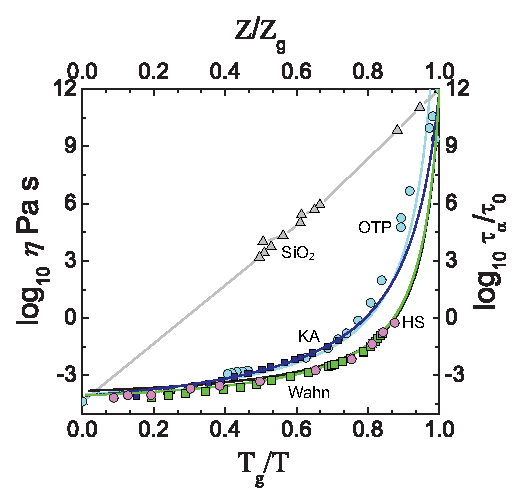
\includegraphics[width=0.9\linewidth,outer]{angell}
  \caption[The Angell plot for model systems undergoing dynamical arrest]{
    The \emph{Angell} plot \cite{AngellJNS1988} for molecular and model glassformers showing the temperature/pressure dependence of viscosity (labelled here as $\eta$) or equivalently relaxation time $\tau_\alpha$.
    The molecular systems \ce{SiO2} and orthoterphenyl (OTP) respectively display the \emph{strong} and \emph{fragile} behaviours described in text, with data obtained from Refs.\ \cite{AngellS1995, BerthierPRE2009}.
    Kob-Anderson (KA) and Wahnstrom (Wahn) are binary mixtures of Lennard-Jones atoms designed to exhibit fragility.
    The compressibility $Z = \beta p / \rho$ is argued to be equivalent to inverse temperature for hard spheres (HS) \cite{BerthierPRE2009}, with data taken from Ref.\ \cite{RoyallJSM2017}.
    Reproduced from Ref.\ \cite{RoyallPR2015}.
  }
  \label{fig:angell}
\end{SCfigure}

Our focus is on soft matter, with hard spheres as the prototypical model, where the  interactions (typically van der Waals attractions) are much weaker than in molecular systems (and absent in hard spheres).
Consequently, there is less of a case for an Arrhenius relationship \eqref{eq:arrhenius-law}, and empirically we find striking deviations from it.
Many systems show \emph{super-Arrhenius} scaling with temperature (Fig.\ \ref{fig:angell}), including mixtures of Lennard-Jones atoms and molecular systems such as orthoterphenyl.
Correspondingly, systems where $\tau_\alpha$ increases more rapidly than exponential are labelled as \emph{fragile}.
A super-Arrhenius scaling of $\tau_\alpha$ implies that the thermodynamic barrier to relaxation $\Delta \Phi_\alpha$ increases with supercooling.
This means that the dynamics fundamentally changes at high densities (or low temperatures), which must be caused by the onset of \emph{collective} (or \emph{cooperative}) effects; given the weakness of bonds in soft matter, we can conclude that many particles must contribute to create a large barrier.
We will discuss this more in the next section.

Some modification is required for hard particle systems, where temperature is not a natural control parameter.
As we argued in the introduction, pressure is the only meaningful state variable.
The authors of Ref.\ \cite{BerthierPRE2009} argue that pressure plays a role equivalent to inverse temperature in athermal systems, because of similarities in their limit behaviour.
Alternatively, we could make a free volume argument, where we expect a relaxation event to involve fluctuations of volume $\Delta V$.
In equilibrium, volume fluctuations are created by reversible work $p \Delta V$ so to leading order%
\marginfootnote{The leading order behaviour can be given more justification by invoking the morphometric approach \eqref{eq:fmt-morphometric-2}, or from more general arguments which we will introduce in section \ref{sec:insertion-as-solvation}.}
we then expect
\begin{equation*}
  \tau_\alpha \sim e^{\beta p \Delta V}.
\end{equation*}
Taking $\Delta V$ as the equivalent of an energy barrier, we find the conjugate variable $\beta p$ does indeed play the role of inverse temperature.
It is usual to work with the dimensionless \emph{compressibility factor}, defined by
\begin{equation}
  Z = \frac{\beta p}{\rho},
\end{equation}
in terms of which hard spheres show the same phenomenology as thermal systems (Fig.\ \ref{fig:angell}); we find that hard spheres are comparable in fragility to various binary Lennard-Jones mixtures.
Relaxation barriers in hard spheres are entropic in nature, so perhaps it is easier to see the need for collective effects.
Moreover, the geometrical interpretation in terms of volume fluctuations $\Delta V$ provides an intuitive picture for collective motion: at high densities more particles have to move out of the way to create space for motion.

\begin{SCfigure}
  \includegraphics[width=0.7\linewidth,outer]{dynamic-heterogeneity}
  \caption[Dynamical heterogeneity in binary hard discs]{
    Dynamical heterogeneity in a binary hard disc system with a size ratio of $1:1.4$.
    Particles are coloured according to distance moved over a relaxation time $\tau_\alpha$, with blue having moved the least and red the most.
    Reproduced from Ref.\ \cite{RoyallPR2015}.
  }
  \label{fig:dynamic-heterogeneities}
\end{SCfigure}

Given the rapid increase in dynamical timescales with supercooling, there comes a point where the relaxation time exceeds the observation time so it is impossible to equilibrate the system.
This is the \emph{experimental glass transition}, operationally set as the point where $\tau_\alpha(T = T_g \textrm{ or } \eta = \eta_g) = \SI{100}{\second}$.
In some sense, this threshold defines a subjective limit of a human observer's patience, and so the point $T_g$ (or $\eta_g$) is not strictly a transition.
However, in practice $\tau_\alpha$ is increasing so rapidly by this point that the location of $T_g$ (or $\eta_g$) is insensitive to the choice of observation time \cite{CavagnaPR2009}.

As the final piece of the phenomenology we introduce two more important dynamical features which differentiates the supercooled liquid from normal liquids.
First, the Stokes-Einstein equation, relating diffusion, temperature and viscosity, holds at high temperatures (low densities) but significant deviations are observed at supercooling to low temperatures (high densities) \cite{BerthierRMP2011}.
This finding possibly suggests the existence of multiple competing relaxation mechanisms in the supercooled liquid, which are probed differently by the two measures \cite{EdigerARPC2000}.
Second, the dynamics becomes highly spatially heterogeneous at increased supercooling (Fig.\ \ref{fig:dynamic-heterogeneities}).
Furthermore, simulation studies have revealed that the initial configuration strongly correlates with the locations of mobile events \cite{Widmer-CooperJPCM2005}.
This suggests that the sites of mobility are encoded in the static configuration, which could be interpreted structurally.
%The size of these hetereogeneities is captured by a dynamic lengthscale $\xi_\mathrm{dyn}$, whereas thermodynamic theories typically concern static lengthscales.
%A requirement of a thermodynamic theory is thus that $\xi_\mathrm{dyn}$ scales with the proposed static length.

%% To unveil static quantities, it is tempting to link dynamical heterogeneity to structural heterogeneity.
%% Stable structures should move less than unstable ones.
%% Widmer-Cooper and Harrowell 11 demonstrated that the initial configuration of a simulation, independently of the initial dynamics, has a role in the heterogeneity of the dynamics.

The main point of contention is over what causes this slow-down: whether it is driven by an underlying phase transition in the thermodynamic viewpoint, or if it is purely a kinetic effect.
The former viewpoint includes the related \emph{mode-coupling} and \emph{random first-order transition} theories, which are loosely based on mean-field theory.
By contrast, the kinetic viewpoint \emph{dynamical facilitation} is based entirely around study of fluctuations.
Having introduced the phenomenology of supercooled liquids we can now proceed to discuss these theories in turn.
We will emphasise the thermodynamic theories because in recent years there has been a substantial shift towards them because of the success of mean-field theories.
Furthermore, our approach focuses on static many-body correlation functions and local structure, which lends itself more towards a thermodynamic viewpoint.

%These are not \emph{completely} mutually exclusive viewpoints, as it is possible hybrid scenarios exist where a phase transition is 

%% We discussed the static correlation functions at length, which is fine for liquids where equilibrium occurs on a \SI{100}{\pico\second} timescale.
%% Dynamical effects are highly nontrivial at high densities.
%% As a practical definition, a glass is defined in the lab as any material for which the relaxation time exceeds \SI{100}{\second}: this point is called the experimental glass transition.
%% This is somewhat arbitrary, although the location of the glass transition point is not particularly sensitive to where you set the threshold because of how rapidly the viscosity/times are increasing around there.
%% So what do we mean by dynamical arrest.

%% Cooling a liquid.
%% Take thermodynamic quantity (e.g.\ volume, entropy, enthalpy): usually crystallise.
%% (Picture)
%% First-order transition bypassed by quick cooling.
%% Enter supercooled liquid phase.

%% Both of these conditions are violated in the glass, as this is a truly non-equilibrium state.
%% That is, we see ageing, and hysteresis in response to perturbations.
%% No longer equilibrates/relax/flows, call it a glass: occurs at glass transition.
%% Glass is a solid for all practical purposes.
%% Distinguished from glass which has dependence on preparation history, hysteresis/memory effect of heating the system (will not follow exactly the same curve until - back to the equilibrium supercooled structure), aging: averages (including correlations) evolve in time.

%% The glass transition itself is not a ``transition'' in the thermodynamic sense; there is no.
%% It's really a kind of impatience transition; the glass transition for a human would be different to the glass transition for a demigod/ent.
%% It's still a relatively robust measurement, because of the superarrhenius scaling (sc-l for pedestrians).

%% A plethora of questions related to the out-of-equilibrium properties.
%% \begin{enumerate}
%% \item Properties of out of equilibrium glass phase: very important questions for material science. Low temperature anomalies, aging behaviour, nonlinear rheology  plasticity.
%% \item Relation between glass and jamming. Jamming=zero temperature, out of equilibrium, infinite pressure.
%% \item How to avoid crystallisation.
%% \end{enumerate}

%% We will talk about this metastable branch as if it were in equilibrium.
%% \todo{create link when mention high density swap data}

%% Relationship with viscosity.
%% Flowing/not flowing is captured by viscosity: viscous slowdown same as relaxation slowdown.
%% Slightly different notion.
%% Short times $t \ll \tau$: elastic system, long times $t \gg \tau$: viscosity.
%% Time barrier is relaxation time.
%% Elasticity, viscosity in Newtonian fluids: viscoelastic behaviour (Maxwell)
%% \begin{equation}
%%   \eta = G_\infty \tau_\mathrm{relax}
%% \end{equation}
%% high frequency shear modulus is elastic property.
%% Shear modulus increases by factor 2-5 times, is dwarfed by change in relaxation time.

\section{Mode-coupling theory}
\label{sec:mct}

The central tenet of mode-coupling theory (MCT) is to separate the liquid's degrees of freedoms into \emph{slow} and \emph{fast} variables.
Fast variables are those that thermalise very quickly, e.g.\ the solvent in a colloidal liquid, so that they can be integrated out leaving only slowly evolving variables of interest.
We advocate essentially the same philosophy, of coarse-graining onto a few dynamically relevant degrees of freedom, in developing a theory for many-body correlations in chapters \ref{chapter:morphometric-framework} and \ref{chapter:morphometric-applications}.
The difference between the two approaches is that MCT explicitly treats \emph{dynamical} processes whereas we focus on \emph{static} correlations.
We will discuss our own approach more in section \ref{sec:correlation-perspective}.

As an example of separation into fast and slow variables, consider classical Langevin equation of motion.
%, which expresses the equations of motion of a subset of the degrees of freedom.
Newton's equation for a particle in an external field becomes
\begin{equation}\label{eq:classical-langevin}
  m \ddot{\vec{r}}
  =
  \vec{\nabla} \phi_\mathrm{ext}(\vec{r})
  - \lambda \dot{\vec{r}} + \vec{f}(t)
\end{equation}
where $m$ is the particle mass, $\lambda$ is a coefficient of damping and $\vec{f}$ is the \emph{fluctuating force} from the fast variables, normally approximated as a Gaussian random field
\begin{equation*}
  \langle f_i(t) f_j(t') \rangle = 2 D \delta_{i,j} \delta(t - t'),
\end{equation*}
with diffusion constant $D$.
Here, the position $\vec{r}$ represents the slowly evolving variable of interest, whereas the remaining degrees of freedom (e.g.\ small solvent particles) are imagined to equilibrate rapidly leaving only the force field $\vec{f}$.

Mode-coupling theory starts from a formally \emph{exact} Langevin equation, which generalises the classical result \eqref{eq:classical-langevin} above.
Defining the instantaneous state of the liquid as
\begin{equation*}
  \vec{X}(t) := \begin{pmatrix} \hat\rho(\vec{r}, t) \\ \vec{\hat{j}}(\vec{r}, t) \end{pmatrix}
\end{equation*}
with instantaneous current $\vec{\hat{j}}(\vec{r}, t) := \partial \hat\rho(\vec{r}, t) / \partial t$, the generalised Langevin equation then reads \cite{ReichmanJSM2005, JanssenFP2018}
\begin{equation}\label{eq:general-langevin}
  \frac{d \vec{\widetilde{X}}(\vec{k}, t)}{dt}
  =
  i \vec{\Omega} \cdot \vec{\widetilde{X}}(\vec{k}, t)
  - \int_0^t \vec{K}(t') \cdot \vec{\widetilde{X}}(\vec{k}, t - t') \, dt'
  + \vec{f}(t)
\end{equation}
where $\vec{f}$ is (again) the fluctuating force obtained by integrating out the fast degrees of freedom, $\vec{K}(t')$ is a time-dependent \emph{memory function} containing the history of $\vec{f}$ as an autocorrelation function \cite{ReichmanJSM2005} and $\vec{\Omega}$ is the \emph{frequency matrix} containing the forces internal to the slow variables \cite{JanssenFP2018}.
Each of these terms has an allegory in the classical Langevin equation \eqref{eq:classical-langevin} above.
Similar equations to \eqref{eq:general-langevin} can be constructed for observables such as the correlation functions; the goal of MCT is to construct (and solve) an equation for $F(\vec{k}, t)$ \eqref{eq:isf} obtaining the dynamical behaviour of the liquid at long times.
The central challenge of this approach is finding suitable approximations for the memory function $\vec{K}$.
%% \begin{equation*}
%%   \vec{K}(t') = \vec{f}(0)^T \vec{f}(t') \cdot (\vec{\widetilde{X}}^T \vec{\widetilde{X}})^{-1}.
%% \end{equation*}

In the standard MCT approach, the fluctuating force is assumed to be dominated by the pair correlations so that $K$ becomes a four-point correlation function.
Then, through a second approximation where $K$ is factorised into a product of two two-point correlation functions, it is possible to construct an evolution equation for the intermediate scattering function \eqref{eq:isf} as \cite{ReichmanJSM2005}
\begin{equation}\label{eq:full-mct}
  \frac{d^2 F(k,t)}{d t^2}
  + \frac{k^2}{\beta m S^{(2)}(k)} F(k, t)
  + \int_0^t K_\mathrm{MCT}(k, t') \frac{d F(k, t - t')}{dt} \, dt'
  =
  0
\end{equation}
with
\begin{subequations}\label{eq:full-mct-coupled}
  \begin{align}
    K_\mathrm{MCT}
    &=
    \frac{\rho}{16 \pi^3 \beta m}
    \int |V_{\vec{q},\vec{k}-\vec{q}}|^2
    F(q, t) F(|\vec{k} - \vec{q}|, t)
    \, d\vec{q},
    \\
    V_{\vec{q},\vec{k}-\vec{q}}
    &=
    \frac{
      \vec{k} \cdot \vec{q} c^{(2)}(q) + \vec{k} \cdot (\vec{k} - \vec{q}) c^{(2)}(|\vec{k} - \vec{q}|)
    }{
      k
    }.
  \end{align}
\end{subequations}
The latter function $V_{\vec{q},\vec{k}-\vec{q}}$ is the so-called \emph{vertex}, which takes the pair direct correlation, and the initial condition for \eqref{eq:full-mct} is $F(k,t=0) = S^{(2)}(k)$; as such, standard MCT takes only pair correlation functions as input.
Together \eqref{eq:full-mct} and \eqref{eq:full-mct-coupled} form a non-linear coupled set of integro-differential equations that can be numerically solved, providing a reasonable description of the \emph{onset} of dynamical arrest, with deviations only becoming noticeable at deep supercooling \cite{FlennerPRE2011,BrambillaPRL2009}.

Crucially, MCT predicts a diverging timescale at $\eta \sim 0.52$ in hard spheres, where the dynamics would become completely arrested, and numerical fits to colloidal experimental data with the same power behaviour law predicted by MCT move this point up to $\eta \sim 0.58$ \cite{VanMegenPRE1994}.
However, this predicted transition must be spurious as recent experiments have managed to equilibrate colloidal hard sphere liquids up to $\eta \lesssim 0.60$ \cite{BrambillaPRL2009,HallettNC2018} and to even higher densities in simulations \cite{BerthierPRL2016}.
Despite this failing of MCT, it remains the only properly first-principles theory for treating liquid dynamics.

Extensions incorporating fluctuations can be found in Refs.\ \cite{BiroliPRL2006,SzamelPTEP2013}, and more recently a generalised MCT has been developed which avoids the uncontrolled factorisation of the pair densities \cite{JanssenPRL2015,JanssenFP2018}.
Importantly, the latter approach incorporates closures of the many-body correlation functions, which will be a central theme of later chapters; by doing this the authors were able to move the diverging timescale to higher densities, bringing the theory into better agreement with available data from simulations and experiments.

\section{Mean-field theories}
\label{sec:mean-field-glass}

We introduced MCT as an explicitly dynamical theory which attempts to model dynamical arrest in supercooled liquids by directly describing the decay of time correlation functions like $F(k, t)$.
Thermodynamics only entered implicitly into MCT through the structural input of the static structure factor $S^{(2)}(k)$.
By contrast, \emph{mean-field theories} of glass take a primarily thermodynamic approach, though they are broadly compatible with the dynamical descriptions of MCT.
The mean-field picture has been rapidly gaining traction in recent years since exact solutions have been developed for hard spheres \cite{ParisiRMP2010,KurchanJSM2012,KurchanJPCB2013,CharbonneauNC2014,CharbonneauJSM2014}.
To describe mean-field theory we will invoke the concept of an \emph{energy landscape}, the natural generalisation of transition state theory introduced in section \ref{sec:glass-phenomenology} and summarised by \eqref{eq:reaction-time}.
While this conceptual framework is not unique to mean-field theories, it is most closely associated with them.

In an energy landscape description, the thermodynamic potential is interpreted \emph{geometrically} as a mapping from every point in configuration space to a `height' representing energy e.g.\ $\Phi: \mathbb{R}^{dN} \mapsto \mathbb{R}$ for an $N$ particle system.
The appeal of this approach is that physical processes can be understood \emph{topographically}: the system will spend more time at the bottom of `valleys' (minima of $\Phi$), especially at lower temperatures, and dynamics will occur primarily through low-lying `mountain passes' (saddles of $\Phi$) \cite{StillingerS1995}.
The timescales of transitions over saddles are expected to scale via the usual Boltzmann weight \eqref{eq:reaction-time}, just as in ordinary transition state theory, however this refined picture emphasises the importance of landscape \emph{connectivity}: the number, separation and relative weights of the various dynamical paths could drive the glass transition.

The energy landscape is particularly relevant in mean-field, formally corresponding to the high dimensional limit%
\marginfootnote{To understand why, consider the typical number of particle neighbours increases with dimensionality.
  Then, formally in the limit $d \to \infty$ a particle is able to achieve a macroscopic number of neighbours, equivalent to an interaction with an average field representing the rest of the system.}
$d \to \infty$, because its \emph{exact} properties can be determined.
In mean-field, hard spheres undergo a \emph{clustering} (or \emph{dynamical}) transition at a volume fraction $\eta_c$ where the landscape splits into disconnected regions \cite{ParisiRMP2010,KurchanJSM2012,KurchanJSM2016}, and the dynamics are described by an almost identical theory to MCT \cite{MaimbourgPRL2016,KurchanJSM2016}.
As configuration space becomes disconnected at $\eta_c$, the system is frozen into a single region and so the relaxation time diverges; contemporaneously, the memory function analogous to $K_\mathrm{MCT}$ in mean-field develops a plateau reflecting the fact that the density profile can no longer completely relax \cite{CharbonneauARCMP2017}.
In this light, the diverging relaxation time predicted by standard MCT is not necessarily a failure of the theory, but is indicative of this genuine mean-field transition.

Although the dynamics is singular at the dynamical transition, the thermodynamic observables are continuous as the system is compressed beyond $\eta_c$ \cite{ParisiRMP2010}.
%% Starting from the definition of the Helmholtz free energy.
%% \begin{equation*}
%%   F = \langle U \rangle - T S.
%% \end{equation*}
We can imagine what happens to the system under further compression if it could continue to sample these disconnected regions in equilibrium, i.e.\ with Boltzmann weighted measure.
The free energy, normally expressed as a sum over all microstates%
\marginfootnote{Which microstates this includes depends on the ensemble.}
$\Gamma$, can be re-expressed as a sum over a collection of \emph{mesostates} $\Gamma = \{\alpha_1, \cdots, \alpha_M\}$ giving
\begin{equation}
%\begin{subequations}
  %\begin{align}
    \Phi = \sum_{i \in \Gamma} p_i \, (\epsilon_i - k_B T \, \ln{p_i})
   % \\
    = \overline{\Phi} - T \Sigma
  %\end{align}
%\end{subequations}
\end{equation}
where $\epsilon_i$ is the energy of microstate $i$ and $p_i$ its probability measure.
In the latter step we defined%
\marginfootnote{This expression is obtained by writing the probability of the system being in mesostate $\alpha$ as $p_\alpha = \sum_{i \in \alpha} p_i$, then $p_i / p_\alpha$ is the probability of microstate $i$ given that the system is in this mesostate.}
\begin{subequations}
  \begin{align}
    \overline{\Phi}
    &=
    \sum_\alpha p_\alpha
    \underbrace{
      \sum_{i \in \alpha} \frac{p_i}{p_\alpha}
      \left(
      \epsilon_i - k_B T \, \ln{\frac{p_i}{p_\alpha}}
      \right)
    }_\textrm{free energy of mesostate $\alpha$},
    \\
    \Sigma &= - k_B \, \sum_\alpha p_\alpha \ln{p_\alpha}.
  \end{align}
\end{subequations}
The \emph{complexity} $\Sigma$ is an extensive quantity characterising the multiplicity of mesostates; at the dynamical transition this becomes a positive non-zero number $\Sigma(\eta = \eta_c) > 0$ corresponding to the clustering in configuration space.
As the system is compressed further $\Sigma$ decreases \cite{KirkpatrickPRB1987,KirkpatrickPRA1989,ParisiRMP2010} corresponding to the rarefaction of clustered regions.
At a volume fraction $\eta_K > \eta_c$ an \emph{entropy crisis} occurs: $\Sigma$ vanishes, leading to the system being frozen into a single, unique region in configuration space called an \emph{ideal glass} phase \cite{KauzmannCR1948,KirkpatrickPRB1987,HallJCP1987,KirkpatrickPRA1989,ParisiRMP2010,BerthierRMP2011}.

If an equilibrium glass state in the regime $\eta \in [\eta_c, \eta_K]$ is compressed out-of-equilibrium without sampling the other clusters, a further phase transition occurs to a so-called \emph{Gardner} phase \cite{KurchanJPCB2013,CharbonneauNC2014,CharbonneauJSM2014}.
Each cluster splits further into fractal sub-regions arranged hierarchically.
Whereas the clustered regions formed at $\eta_c$ are geometrically dissimilar%
\marginfootnote{As measured by e.g.\ the intermediate scattering function},
these regions are close in configuration space to one another.
This phase has deep connections with the jamming transition seen at diverging pressure, providing a unified description of glass and jamming conjectured since the landmark paper of Ref.\ \cite{LiuN1998}.
Remarkably, this mean-field theory is able to predict anomalous $d$-independent critical scaling coefficients, matching those known around jamming \cite{WyartPRL2012,LernerSM2013,DeGiuliPNAS2014}.
The existence of the Gardner phase provides context for the importance of mean-field theory, but it cannot be directly connected to our approach in subsequent chapters so we will not discuss it further.
For more information on the mean-field Gardner phase see the reviews of Refs. \cite{BerthierJCP2019,CharbonneauARCMP2017}.

%% Specifically, the glass transition can be understood as the division of the energy landscape up into subunits??
%% Exact properties of the energy landscape can be determined for many mean-field systems, where it is known to play a leading role in dynamical arrest.

The mean-field picture introduces complexity as the important quantity of interest, relating the number of metastable regions in configuration space.
The relevance of mean-field descriptions in physical dimensions requires a finite-dimensional description of the supercooled liquid and its energy landscape.

%% In physical dimensions, the energy landscape does not become completely disconnected, so transitions between metastable states are possible; the dynamical transition becomes a cross-over.
%% As such, a finite-dimensional description of the supercooled liquid is needed.

%% In physical dimensions, the energy landscape does not become
%% This quantity is well-defined in mean-field because these regions are completely disconnected, however in finite dimensions transitions can always occur between them through nucleation \cite{KirkpatrickPRB1987,KirkpatrickPRA1989,BouchaudJCP2004}.
%% The dynamical transition thus becomes a cross-over, and a finite-dimensional description of the supercooled liquid is needed.

\section{Finite-dimensional theories}
\label{sec:finite-d-glass}

\begin{SCfigure}
  \includegraphics[width=0.9\linewidth,outer]{swap-Sconf}
  \caption[Configurational entropy in hard spheres from Monte-Carlo simulations]{
    Configurational entropy in hard spheres from novel Monte-Carlo (MC) simulations for a system with 23\% polydispersity.
    $Z_0 \approx 18$ ($\eta_0 \approx 0.56$) marks the onset pressure, above which the intermediate scattering function $F(k,t)$ decays non-exponentially, and $Z_c \approx 23.5$ ($\eta_c \approx 0.598$) is the location of the dynamical transition predicted by fitting mode-coupling theory's power-law scaling to the lower density behaviour.
    The various methods used (described in Ref.\ \cite{BerthierPNAS2017}) all broadly agree that this quantity is trending to zero at a finite pressure, suggesting the existence of a thermodynamic glass transition.
    The equation of state for this system is given in Fig.\ \ref{fig:swap-eos}.
    Reproduced from Ref.\ \cite{BerthierPNAS2017}.
  }
  \label{fig:swap-sconf}
\end{SCfigure}

%% Mean-field theories have traditionally been formulated in configuration space, in terms of the energy landscape.
%% By contast, in $d=3$ the existence of dynamical heterogeneity calls for a real space interpretation.

The relevance of mean-field ideas in physical dimensions can be seen by an interpretation of Refs.\ \cite{KirkpatrickPRB1987,HallJCP1987,KirkpatrickPRA1989}, with antecedent ideas found in \cite{KauzmannCR1948,AdamJCP1965}.
This \emph{random first-order transition} (RFOT) scenario acknowledges that the clustering of states appearing at the dynamical transition in mean-field will not be strictly metastable over finite lengthscales in finite $d$ \cite{BouchaudJCP2004,MontanariJSP2006}.
As such, the complexity is not well-defined because the metastable states will not be strictly separated with infinite barriers, though they may be arbitrarily long-lived; the dynamical transition of mean-field thus becomes a cross-over.
In finite dimensions, the \emph{configurational entropy} $S_\mathrm{conf}$ is introduced as the closest equivalent to the complexity; this does not have a generally agreed upon meaning, but a common definition invokes the timescale separation between vibrational ($\beta$--) and liquid-like ($\alpha$--) dynamics.
The configurational entropy then describes the entropy of the latter process, obtained as the residual entropy after removing vibrations
\begin{equation}\label{eq:sconf}
  S_\mathrm{conf} := S - S_\mathrm{vib},
\end{equation}
though some refinement is required for polydisperse systems \cite{OzawaJCP2017,OzawaJCP2018} and where additional non-vibrational processes exist that do not relax the density profile \cite{OzawaPRL2018}.

The RFOT scenario imagines the mean-field dynamical transition as a crossover to an \emph{energy landscape dominated} dynamics.
Specifically, the number of unique (non-vibrational) states possible in a subregion of size $\xi$ will scale $\propto \exp{(s_\mathrm{conf} \xi^d / k_B)}$, where $s_\mathrm{conf} = S_\mathrm{conf} / V$ is the configurational entropy density.
A dynamical event which changes a state is expected to pay an energy penalty $\gamma_\mathrm{eff} \xi^\theta$ where $\theta \le d$ from inducing a mismatch with the surrounding fluid.
The thermodynamic potential for this subregion is then expected to adopt the form
\begin{equation}\label{eq:rfot-barrier}
  \Phi \sim \gamma_\mathrm{eff} \xi^\theta - T s_\mathrm{conf} \, \xi^d.
\end{equation}
The maximum of $\Phi$ occurs at the \emph{point-to-set}%
\marginfootnote{So-named because this lengthscale marks the crossover from the subregion being confined to a single `point' in its configuration space to a `set' of states.}
length
\begin{equation}\label{eq:rfot-xi}
  \xi_\mathrm{PS}
  := \argmax{(\Phi)}
  \sim
  \left(
  \frac{\theta \gamma_\mathrm{eff}}{d T s_\mathrm{conf}}
  \right)^\frac{1}{d-\theta},
\end{equation}
after which $\Phi$ grows infinitely negative, so the metastable states are unstable to activated dynamics for $\xi \gtrsim \xi_\mathrm{PS}$.
The RFOT interpretation thus predicts the formation of a \emph{mosaic} of droplets of typical lengthscale $\xi_\mathrm{PS}$ \cite{KirkpatrickPRB1987,HallJCP1987,KirkpatrickPRA1989,BouchaudJCP2004}.
The nature of the entropic droplets forming the mosaic state and the processes by which they relax is an active area of study \cite{BouchaudJCP2004,DzeroPRB2005,FranzJSM2005,AngeliniJSP2017,RulquinJSM2016,BiroliMeanPRB2018,BiroliFinitePRB2018}.
Notably, a lot of attention has been devoted to the treatment of the subleading term $\gamma_\mathrm{eff} \xi^\theta$.

This thermodynamic argument above concerns whether a region of the liquid \emph{will} relax eventually, but an even more direct connection with relaxation timescale was proven in Ref.\ \cite{MontanariJSP2006}.
Briefly, dynamical barriers must remain finite within a finite subregion, so they scale Arrheniusly via \eqref{eq:reaction-time}; any Arrhenius process will eventually overwhelm the super-Arrhenius scaling of $\tau_\alpha$ at deep supercooling.
Fragile behaviour then suggests a reduction in $S_\mathrm{conf}$ to limit the number of possible Arrhenius processes.
Moreover, the authors of Ref.\ \cite{MontanariJSP2006} then show that the relaxation time is rigorously bounded from above by $S_\mathrm{conf}$, proving that any diverging relaxation time \emph{must} coincide with an entropy crisis where $S_\mathrm{conf}$ becomes sub-extensive.
Measurements of the configurational entropy from simulations of hard spheres suggest a vanishing $S_\mathrm{conf}$ at finite pressure in $d=3$ (Fig.\ \ref{fig:swap-sconf}), pointing to a mean-field/RFOT scenario in hard spheres.
However, this necessarily relies on extrapolation as the point where $S_\mathrm{conf}$ vanishes cannot be reached in finite time because of the argument above.

%% Mean-field argument is thermodynamic, which in some sense is structural.
%% Structural in the sense of the energy landscape, not necessarily in real space/local structure.
%% The real space interpretation of mean-field theory is random first-order transition theory (RFOT), also called \emph{mosaic} theory.

%% In conventional condensed matter physics dynamics is determined by structure.
%% For example, crystalline solids are fixed on a lattice so do not flow, whereas liquids are disordered and are thus able to flow.
%% Soft matter systems (e.g.\ gels, foams, glasses) do not neatly fall into this paradigm: their dynamics are often arrested whilst their structure remains highly disordered.

\begin{SCfigure}
  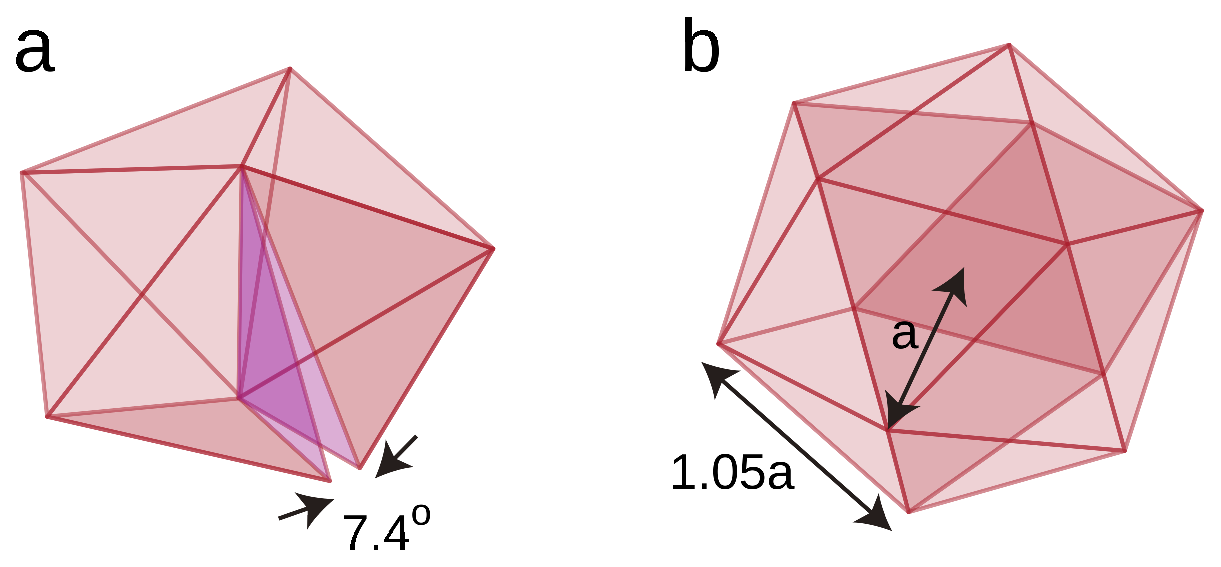
\includegraphics[width=0.7\linewidth,outer]{frustration}
  \caption[Frustration of tetrahedral structures]{
    Structures formed by combining tetrahedra.
    (a) The pentagonal bipyramid constructed from five regular tetrahedra must leave a small gap of \SI{7.4}{\degree}.
    (b) The icosahedron formed by vertices a distance $a$ from the centroid must have edge length $\sim1.05 a$, so if hard spheres of diameter $a$ were placed on the vertices they would not be in contact.
    Reproduced from Ref.\ \cite{RoyallPR2015}.
  }
  \label{fig:frustration}
\end{SCfigure}

A different scenario in physical dimensions focuses on the role of geometry.
This picture starts from the observation that crystal structures (e.g.\ the face-centred cubic introduced for hard spheres at close packing) are generally not the optimal energetic arrangement for small clusters of particles, even though they must be for bulk systems.
For example, 13 isolated Lennard-Jones atoms will preferentially arrange as vertices of a fivefold symmetric \emph{icosahedron} \cite{FrankPRS1952} (Fig.\ \ref{fig:frustration}b).
As fivefold symmetric structures cannot tessellate Euclidean space, Sir Charles Frank conjectured that glassformers suppress crystallisation through formation of icosahedra (or similar structures) \cite{FrankPRS1952}.

The above viewpoint has been developed into the more complete theory called \emph{geometric frustration} \cite{KivelsonPA1995,TarjusJPCM2005}.
This approach characterises the liquid by its \emph{locally favoured structures} (LFS), i.e.\ those structures which are energetically favoured at small length scales.
A system could have a single LFS, or a whole collection; recently, it has been shown through numerical simulations that \emph{competition} between different LFS enhances the propensity for glassformation \cite{TeichNC2019}.
This competition is an example of \emph{frustration} where continual growth of domains of LFS is hindered by geometric constraints.
Frustration can also emerge from a single LFS if it cannot tile space, as is the case of fivefold symmetric structures like icosahedra.
Incorporating frustration into a theory modelling the energy of LFS-rich domains leads to a similar scaling relation as in RFOT \eqref{eq:rfot-barrier}, though the resulting phase behaviour is quite different.
The static lengthscale which emerges from this theory is interpreted as the size of the domains, which is more easily understood than the amorphous lengthscale $\xi_\mathrm{PS}$ of RFOT.
Details can be found in the review of Ref.\ \cite{TarjusJPCM2005}.

The frustration picture is broadly compatible with the mean-field viewpoint: the propensity for a system to form certain structures can be interpreted as a manifestation (or a driving force) of a reduced $S_\mathrm{conf}$.
The downside of this scenario is that the correlation between local structure and dynamics seems to be highly system dependent \cite{HockyPRL2014}.

Whereas RFOT postulates amorphous order, geometric ideas propose simpler static orderings based around e.g.\ LFS domains.

CPR: local structure fixes gel \cite{RoyallNM2008}.
Charbonneau: growth of length scale associated with LFS does not correlate with dynamical length scale \cite{CharbonneauPRL2012}, possibly multiple relaxation mechanisms or a non-static length scale.
Leacmach: \cite{LeocmachNC2012}
Coslovich: \cite{CoslovichJCP2007,CoslovichJCP2007a}
Turci: \cite{TurciPRL2017}

In hard spheres, the dominant LFS are found to be icosahedral motifs in accordance with Frank's original conjecture.
In Fig.\ \ref{fig:icosahedral-domains} we see the growth of large domains of icosahedra in the supercooled liquid, over a range in densities where $\tau_\alpha$ changes by a factor of $\mathcal{O}(10^5)$ (Fig.\ \ref{fig:g2-changes}) \cite{HallettNC2018}.
This fact demonstrates that significant structural change occurs alongside dynamical arrest, even though minimal changes are seen at the pair level.
This does not prove that structural change \emph{causes} the slowdown, but it does suggest the idea is worth investigating.
%Furthermore, the vicinity of an icosahedral motif is found to be highly correlated with local particle mobility \cite{HallettNC2018}.

%At high densities the tetrahedra form large connected domains \cite{HallettNC2018} rich in fivefold symmetric structures.
Spherical packings ideally form regular tetrahedra which cannot perfectly form pentagonal structures (Fig.\ \ref{fig:frustration}), so fivefold symmetric structures are highly frustrated.
A detailed review on the role of local structure in glassy systems can be found in Ref.\ \cite{RoyallPR2015}.
\todo{Should definitely cite more Royall group work here, possibly Tanaka too. What's the most appropriate cross-section of papers?}

%% The mean-field picture of glass formation interprets the dynamical slowdown entirely within a thermodynamic framework.
%% In mean-field hard spheres, formally in the limit of infinite spatial dimensions $d \to \infty$,
%% Hard spheres in mean field have been shown to have a thermodynamic glass transition, however the critical dimensions are unknown so it is unclear what happens in $d=3$. \cite{ParisiRMP2010,KurchanJSM2012,KurchanJPCB2013,CharbonneauNC2014,CharbonneauJSM2014}.
Recent numerical evidence suggests that $S_\mathrm{conf}$ only vanishes at $T=\SI{0}{\kelvin}$ for a model glassformer in $d=2$ \cite{BerthierNC2019}.
As this point cannot be crossed no thermodynamic transition can occur in $d = 2$, pointing to a lower critical dimension for mean-field theory of at least $d_L \ge 2$.
It is possible that low-dimensional fluctuations prevent any thermodynamic transition, and it has been argued that even if there is a thermodynamic transition at $\eta_K$ this may not be responsible for the dynamic slowdown seen around the operational glass transition $\eta_g \ll \eta_K$ \cite{WyartPRL2017}.
As such, there is room for alternative pictures to the mean-field/RFOT scenario.

The main opposition theory is \emph{dynamic facilitation}, which focuses on the dynamic heterogeneities as the fundamental feature of glass.
In this picture dynamical events occur through string-like motion between dynamical defects, and the relaxation time remains finite until $T = \SI{0}{\kelvin}$.
\todo{Paddy: Expand on this substantially}
For more information on dynamic facilitation we direct the reader to the review of Ref.\ \cite{ChandlerARPC2010}.
%This must trivially occur at the very least $T=0\si{K}$ where relaxation timescales diverges, however much like the lack of a phase transition in the Ising model in $d=1$ this is not a true thermodynamic phase transition because it cannot be crossed.
%So the central question of glass is what happens in $d=3$, is there a vanishing configurational entropy at a finite $T > 0$ with an accompanying thermodynamic glass transition?

%Theories concentrating on the high density glass: elastic theories.

\begin{SCfigure}
  \includegraphics[width=\linewidth,outer]{icosahedra-hallett}
  \caption[Growth of icosahedral domains in the supercooled hard sphere liquid]{
    Growth of icosahedral domains in a colloidal hard sphere liquid with supercooling, i.e.\ increased volume fraction $\eta$, over a density change which coincides with minimal structural change at the pair level (Fig.\ \ref{fig:g2-changes}).
    (a) STED nanoscopy image for $\eta = 0.598$, with scale bar \SI{3}{\micro\meter}.
    (b), (c) Rendered coordinates of partial icosahedra (green, top right structure) and full icosahedra (purple, bottom right structure) for volume fractions (b) $\eta = 0.523$ and (c) $\eta = 0.598$.
    Reproduced from Ref.\ \cite{HallettNC2018}.
  }
  \label{fig:icosahedral-domains}
\end{SCfigure}

\section{Perspective: usefulness of many-body correlations}
\label{sec:correlation-perspective}

In subsequent chapters will be heavily focusing on the treatment of static many-body correlation functions in the bulk liquid.
Here, we motivate their study for the treatment of the supercooled liquid.
It is natural to wonder what new information can be obtained from the many-body correlation functions that is not already present at the pair level.
In section \ref{sec:thermodynamic-routes} we saw how the compressibility and virial routes lead to expressions of the free energy in terms of pair correlations.
This is emblematic of conventional routes to the free energy, so in some sense all of the thermodynamically relevant information is contained in the two body correlation functions.

Firstly, while it is true that thermodynamic quantities like the pressure can certainly be inferred from the pair correlations, there is no such simple relationship for dynamical quantities.
In the absence of a thermodynamic phase transition, we would not expect the pair correlation function alone to reveal much about the nature of dynamical arrest, beyond the lack of a transition.
Even supposing the existence of a transition, the precision required to detect such a signal $g^{(2)}(r)$ may be arbitrarily subtle; however, any changes approaching a transition \emph{must} be magnified at the many-body level because of \eqref{eq:correlation-derivatives}.
The many-body correlation functions have potential to place the entropic droplet scenario of \eqref{eq:rfot-barrier} on more rigorous footing, by providing a means to calculate the subleading penalty term $\gamma_\mathrm{eff} \xi^\theta$.
Alternatively, the theories which postulate local mechanisms such as the LFS in geometrical viewpoints or the dynamical defects in facilitation should be identifiable within the many-body correlation functions.

Secondly, even at the thermodynamic level the many-body correlations have advantages.
To illustrate this we borrow an argument originally made by Evans \cite{EvansPrivate2019}.
Pair correlations yield thermodynamic quantities which are \emph{derivatives} of the free energy at an instantaneous state point, so to infer the free energy multiple state points must be sampled.
Equivalently, we could consider the derivatives of the pair correlation function.
It is straightforward to show that \cite{Santos2016}
\begin{equation}\label{eq:correlation-derivatives}
  \chi_T \rho
  \left( \frac{\partial \rho^{(n)}}{\partial \rho} \right)_{V,T}
  =
  (n - \rho V) \rho^{(n)}(\vec{r}^n)
  + \int \rho^{(n+1)}(\vec{r}^{n+1}) \, d\vec{r}_{n+1}.
\end{equation}
The important feature to take away from this expression is the presence of $\rho^{(n+1)}$; we see the emergence of higher-order correlation functions in the derivatives.
This means we could in principle measure the free energy at a single state point by introducing highly accurate measurements of the many-body correlation functions.
This is essentially the spirit of the \emph{entropy route}, which writes \cite{WallaceJCP1987}
\begin{equation}
  S = \sum_{n=1}^\infty S_n
\end{equation}
with entropic terms $S_n$ containing contributions from $n$-particle correlations.
The first few terms are given by \cite{WallaceJCP1987}
\begin{subequations}
  \begin{align}
    \frac{S_1}{V}%\langle N \rangle}
    &=
    k_B \, \rho \left( \frac{d}{2} - \ln{\rho \Lambda^d} \right),
    \\
    \frac{S_2}{V}%\langle N \rangle}
    &=
    \frac{\rho^2}{2 T}
    \int g^{(2)}(\vec{r}) \ln{g^{(2)}(\vec{r})}
    \, d\vec{r},
    \\
    \frac{S_3}{V}%\langle N \rangle}
    &=
    \frac{\rho^3}{6 T}
    %\int g^{(3)}(\vec{r}, \vec{r}') \delta w^{(3)}(\vec{r}, \vec{r}')
    \int g^{(3)}(\vec{r}, \vec{r}')
    \ln{\left(
      \frac{
        g^{(3)}(\vec{r}, \vec{r}')
      }{
        g^{(2)}(\vec{r}) g^{(2)}(\vec{r}') g^{(2)}(\vec{r} - \vec{r}')
      }
      \right)}
    \, d\vec{r} d\vec{r}'.
  \end{align}
\end{subequations}
Then, for a pair-interacting system the excess free energy is obtained as
\begin{equation*}
  \begin{split}
    \frac{\beta F^\mathrm{ex}}{V}
    =& \; \hphantom{ + } \;\,
    \frac{\rho^2}{2} \int g^{(2)}(\vec{r})
    \left( \beta u(\vec{r}) - \ln{g^{(2)}(\vec{r})} \right)
    d\vec{r}
    \\ & \;
    + \frac{\rho^3}{6}
    %\int g^{(3)}(\vec{r}, \vec{r}') \delta w^{(3)}(\vec{r}, \vec{r}')
    \int g^{(3)}(\vec{r}, \vec{r}')
    \ln{\left(
      \frac{
        g^{(3)}(\vec{r}, \vec{r}')
      }{
        g^{(2)}(\vec{r}) g^{(2)}(\vec{r}') g^{(2)}(\vec{r} - \vec{r}')
      }
      \right)}
    \, d\vec{r} d\vec{r}'
    \\ & \;
    + \mathcal{O}\left( \rho^4 g^{(4)}(\vec{r}, \vec{r}', \vec{r}'') \right),
  \end{split}
\end{equation*}
so the free energy can be directly obtained from accurate determination of the correlation functions.
%Similarly, a theory treating the many-body correlation functions must have the free energy (and phase behaviour) built in.

We will be focusing on many-body correlations in real space, to explore the local mechanisms proposed in theories of the glass transition described above.
In some situations the correlations in Fourier space may be more useful, most notably in MCT where many-body generalisations have already found some traction \cite{JanssenPRL2015,JanssenFP2018}.
In principle, our real space correlation functions can be Fourier transformed to obtain these, but in practice this is prohibitively expensive because of the high dimensionality of the arguments for even modest values of $n$.
However, FMT already provides an easy route to obtaining all the correlation functions in Fourier space, as described by the original papers \cite{RosenfeldPRL1989,RosenfeldJCP1990}.
We show how to obtain these below.

Fourier transforming the direct correlation functions for the uniform liquid \eqref{eq:fmt-direct-correlations-uniform-density}, and applying the convolution theorem, allows us to write the rather succinct
\begin{equation}
  \widetilde{c}^{(n)}(\vec{k}^n)
  =
  - \sum_{\alpha_1, \alpha_2, \cdots, \alpha_n}
  \partial^n_{\alpha_1, \alpha_2, \cdots, \alpha_n} \beta f^\mathrm{ex} \;
  \left( \prod_{i=1}^n \widetilde{\omega}_{\alpha_i}(\vec{k}_i) \right)
  \delta(\vec{k}_1 + \vec{k}_2 + \cdots + \vec{k}_n).
\end{equation}
The delta function enforces the `ring' condition $\sum_{i=1}^n \vec{k}_i = 0$ which emerges from translational symmetry of the weight functions, reducing the dimensionality of the domain by $d$.
A further $d(d-1)/2$ degrees of freedom%
\marginfootnote{This many degrees of freedom can be removed for general $n \ge d$, but we expect fewer for $n < d$.
  For example, $n=2$ arrangements (a dimer) are isomorphic to a line so they possess $d-1$ rotational degrees of freedom.}
can be removed by exploiting rotational symmetry.
Many-particle generalisations of the static structure factor can be obtained from $\widetilde{c}^{(n)}(\vec{k}^n)$ by functionally differentiating the Ornstein-Zernike equation \eqref{eq:ornstein-zernike-generic} with respect to density \cite{BarratMP1988}.

\section{Summary}

This concludes the relevant background in supercooled liquids and glasses.
In subsequent chapters we will develop a framework for treating the many-body correlation functions in real space, with the hope that it can address some of the questions outlined here.
\todo{More more more, according to Paddy. ``What does it all mean?'' Static lengthscales $=n$}

\ifdefined\includebibliography
  \newgeometry{margin=1in}
  \printbibliography
\fi

\end{document}

\documentclass[12pt]{report}
\usepackage{preamble}
\setcounter{chapter}{2}

\begin{document}
\chapter{Morphological framework for many-body correlations}
Mostly theoretical but with some numerical experiments which motivate/justify developments to the theory.
The main body of numerical work is left to the following chapter.

\section{Formalism for many-body correlations}
A generalised potential distribution theorem and the potential of mean force.

\section{Morphological form of the potential of mean force}
Justification of assumptions: additivity, continuity and motion invariance
\subsection{Limitations known from DFT literature}
\subsection{As a generalisation of scaled particle theory}
And the limitations this implies.

\section{Worked examples where morphometric form can be exact}
Under certain conditions.
\subsection{Low density limit in arbitrary dimensions from lowest order terms in the virial expansion of the pressure}
\subsection{Arbitrary densities at large lengthscales}
\subsection{Hard rods (dimension d = 1) at all densities}
\subsubsection{Exact result from DFT}
\subsubsection{Morphometric result}
Explore where additivity, continuity and motion invariance apply.
\subsubsection{Implications for higher dimensions}

\section{Derivation of thermodynamic coefficients for hard spheres in $d = 3$}

\section{Accuracy of predicted distribution functions in $d = 3$}
\subsection{Comparison with molecular dynamics simulations}
\subsection{Comparison with Kirkwood superposition approximation}

\end{document}

%TC: macro \marginfootnote [other]
%TC: envir SCfigure [] other
%TC: macrocount beginSCfigure [figure]
\documentclass[11pt,twoside]{report}
\usepackage{preamble}
\setcounter{chapter}{3}
\graphicspath{{../img/}}
\def\includebibliography{}

\externaldocument{background}
\externaldocument{morphometric-framework}

\begin{document}
\chapter{Local structure in the hard sphere liquid}
\epigraph{\textbf{hardball 1.1} \emph{informal} Uncompromising and ruthless methods or dealings.}{Oxford English Dictionary}
\label{chapter:morphometric-applications}
\todo{Check which version of dictionary.}

The majority of this chapter contains work published as Ref.\ \cite{RobinsonPRL2019}.
Later stuff is new.

\section{Introduction}

While mean-field theories provide insight into complex phenomena, physical accuracy is ensured only by a proper treatment of correlations.
For example, the simplest case of two-body correlations is at the foundation of predictive theories of the liquid state \cite{Hansen2013}, colloids, and complex plasmas \cite{LikosPR2001,Ivlev2012}.
%, and some forms of active matter \cite{Bechinger2016}.
In particular, the thermodynamics of simple liquids with solely pairwise interactions can be exactly expressed in terms of two-body correlations \cite{Hansen2013}.
However, to resolve these integrated quantities \emph{spatially} into structural motifs, and \emph{temporally} into specific dynamical events, one needs to calculate many-body correlations.
While such a many-body approach may often be neglected in normal liquids, long-standing challenges such as the dramatic dynamical changes occurring in supercooled liquids approaching their glass transition \cite{BerthierRMP2011,RoyallPR2015} and phase transitions such as crystal nucleation \cite{RussoSR2012} call for a many-body description.

In the case of supercooled liquids, theories based on pair correlations such as the standard mode-coupling framework \cite{goetze} fail to account for activated events thus predicting a spurious ergodicity breaking transition \cite{BrambillaPRL2009,HallettNC2018}.
Activated dynamics are often rationalised through collective (i.e.\ many-body) effects within contrasting thermodynamic and purely dynamic scenarios \cite{LubchenkoARPC2007,TarjusJPCM2005,BiroliPRL2006,JanssenPRL2015,SzamelPTEP2013,ChandlerARPC2010}.
These include exact mean-field results in high dimensions \cite{ParisiRMP2010,CharbonneauARCMP2017} whose relevance in finite-dimensional systems is hotly debated \cite{WyartPRL2017}.
A finite-dimensional theoretical description of many-body effects is therefore much needed.

However, many-body correlations are challenging to compute and typically combine both energetic and entropic contributions.
Physical insight can be gleaned by exploring the potential energy landscape of isolated clusters \cite{Wales2004,ArkusPRL2009}, but such methods are only exhaustive for small system sizes.
This limitation has been partly addressed by embedding clusters in a mean-field approximation of the surrounding liquid \cite{MossaJCP2003,MossaJNS2006}.
\todo{Describe Mossa and Tarjus approach in detail.}
Nonetheless, this approach neglects by construction the intra-cluster entropic contributions that may dominate in the supercooled regime of interest.
Furthermore, computer simulations, which naturally deliver full many-body correlations are limited in the range of dynamics they can access, hampering an approach to the glass transition, except for recent developments for certain models \cite{BerthierPRL2016}.

Here we place theoretical predictions of many-body local structure on a fundamentally more rigorous footing using inhomogeneous liquid state theory \cite{EvansAP1979}, which we reviewed in section \ref{sec:dft} and advanced in the chapter \ref{chapter:morphometric-framework}.
We model the many-body interactions between a local subsystem and the remaining liquid, directly accessing the many-body \textit{free} energy of local arrangements of particles.
This allows us to predict the populations of specific local structures in the bulk system across the entire liquid phase and beyond the dynamically accessible supercooled regime.
\todo{Make clear that in terms of glassy theories our approach does lean more towards a local structure point of view.}

\section{Many-body correlations and surface tension}

We conceptually separate the liquid into $n$ spatially adjacent particles and the remaining degrees of freedom, acting as a solvent, which we treat within the grand-canonical ensemble, as sketched in Fig.\ \ref{fig:system}(a).
The joint probability density for simultaneously finding $n$ identical particles embedded in $\mathbb{R}^d$ at positions $\vec{r}^n := \{\vec{r}_1, \dots, \vec{r}_n\}$ \todo{Move this definition to an earlier chapter} is proportional to the \emph{$n$-particle distribution function} $g^{(n)}(\vec{r}^n)$ \cite{Hansen2013}.
For a homogeneous system, this can be formally expressed in terms of the \emph{potential of mean force}, the reversible work required to insert the particles at $\vec{r}^n$:
\begin{equation}\label{eq:potential-mean-force}
  \begin{split}
    \phi^{(n)}(\vec{r}^n) &\equiv - k_B T \ln g^{(n)}(\vec{r}^n) \\
    &= U(\vec{r}^n) + \Delta \Omega(\vec{r}^n) - n\mu^{ex}.
  \end{split}
\end{equation}
We denote by $U$ the total potential energy of the $n$ interacting particles and by $\Delta\Omega := \Omega - \Omega_\textrm{hom}$ the difference between the grand potential of the homogeneous liquid $\Omega_\textrm{hom}$ (related to the total volume and pressure by the relation $\Omega_\textrm{hom} = -pV$) and the grand potential of the system including the $n$-particle inhomogeneity.
Finally, $k_B T$ and $\mu^{ex}$ are the thermal energy and the excess chemical potential (with respect to the ideal gas) of the homogeneous liquid respectively.

For systems with excluded volume interactions, we can divide the space into a local component $\mathcal{L} \subset \mathbb{R}^d$ of volume $V_\mathcal{L}$ inaccessible to solvent degrees of freedom and the remaining space $\mathcal{R} = \mathbb{R}^d \setminus \mathcal{L}$ filled by solvent (Fig. \ref{fig:system}).
The dividing surface $\partial\mathcal{L}$ separates these two components with surface area $A_{\partial\mathcal{L}}$, creating a surface tension $\gamma$.
The solvent contribution to Eq.\ \eqref{eq:potential-mean-force} is then \begin{equation}\label{eq:surface-tension}
  \Delta \Omega[\mathcal{L}] =
  p V_\mathcal{L} + \gamma[{\partial\mathcal{L}}] A_{\partial\mathcal{L}}.
\end{equation}
Note that the surface tension is not unique as only the total grand potential must be independent of the choice of $\partial\mathcal{L}$ and can even change its sign for some choices of dividing surface \cite{BrykPRE2003}.
For simplicity we will consider one-component liquids with particles of diameter $\sigma$.
Letting $B_R(\vec{r}_i)$ denote a ball of radius $R$ at site $\vec{r}_i$, we choose the \emph{solvent accessible surface} \cite{LeeJMB1971} as the dividing surface such that $\mathcal{L} = \cup_{i=1}^n B_\sigma(\vec{r}_i)$ (Fig.\ \ref{fig:system}).

Following Ref.\ \cite{KonigPRL2004} we assume $\Delta\Omega$ is translation and rotation invariant, continuous (with respect to the Hausdorff metric), and additive.
Hadwiger's characterisation theorem \cite{Hadwiger1957} then ensures the surface tension adopts the so-called \emph{morphometric} form
\begin{equation}\label{eq:morphometric-surface-tension}
  \gamma[\partial\mathcal{L}] =
  \gamma_\infty +
  \frac{\kappa \, C_{\partial\mathcal{L}} + \overline{\kappa} \, X_{\partial\mathcal{L}}}
       {A_{\partial\mathcal{L}}},
\end{equation}
with integrated mean and Gaussian curvatures $C_{\partial\mathcal{L}}$ and $X_{\partial\mathcal{L}}$, and $\gamma_\infty,\kappa,\overline{\kappa}$ as thermodynamic coefficients to be determined.
$\gamma_\infty$ is the surface tension at a planar wall (i.e.\ the familiar macroscopic surface tension), whilst $\kappa$ and $\overline{\kappa}$ are ``bending energies'' accounting for curvature corrections occurring at small length scales.
These values are system (and state point) dependent, but do not depend on the local geometry, making the linear form of Eq.\ \eqref{eq:morphometric-surface-tension} desirable for calculation.
While strictly an approximation, we motivate Eq.\ \eqref{eq:morphometric-surface-tension} from numerical studies where it has been found to be highly accurate below the freezing volume fraction in hard spheres \cite{RothPRL2006,LairdPRE2012,BlokhuisPRE2013,UrrutiaPRE2014,Hansen-GoosJCP2014}, and from the early success of scaled particle theories \cite{ReissJCP1959,ReissJCP1960}.

\begin{SCfigure}
  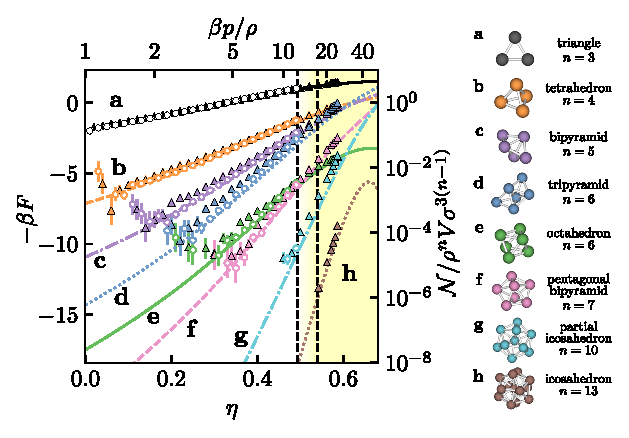
\includegraphics[width=\linewidth,center]{structure-populations}
  \caption[Concentration of local structures in the equilibrium liquid]{
    Static many-body structure in the hard sphere liquid: populations of small local structures in the hard sphere liquid determined from molecular dynamics simulations of 1372 monodisperse (open circles) and 8\% polydisperse (solid triangles) hard spheres against the theoretical prediction of this work (lines).
    Variations against volume fraction $\eta$ and compressibility $Z = \beta p/\rho$ shown.
    The hard sphere freezing and melting volume fractions are indicated by vertical dashed lines.
  }
  \label{fig:structure-populations}
\end{SCfigure}

\begin{SCfigure}
  \includegraphics[width=0.9\linewidth,outer]{n12-dos}
  \caption[Free energy distribution of 12 particle structures]{
    Theoretical free energy distribution for the $n=12$ local library of states at several volume fractions.
    The distribution is shifted to lower energies at higher volume fractions, and develops an increasingly bimodal structure.
    Populations are decomposed into those structures containing pentagonal bipyramids without octahedra (light fill) and the remaining structures (dark fill).
  }
  \label{fig:n12-dos}
\end{SCfigure}

\emph{Existing morphological theories.}---We focus on the hard sphere system because of its fundamental interest in the theory of liquids \cite{WidomS1967,Hansen2013}.
This allows suitable coefficients of Eq.\ \eqref{eq:morphometric-surface-tension} to be derived analytically by exploiting the geometric nature of hard spheres.
We compute morphological quantities and their derivatives following Ref.\ \cite{KleninJCC2011}, which we have extended to calculate curvature measures [see details in the Supplementary Material (SM)].
Note that hard spheres are athermal meaning density is the only control parameter and all free energies are really entropies; here we use ``supercooled'' to mean high density.

We assume the Carnahan-Starling (CS) equation of state \eqref{eq:cs-pressure} \cite{CarnahanJCP1969} because this pressure is used in the WBII theory and is accurate deep within the supercooled regime \cite{BerthierPRL2016} although it will fail at very large densities nearing random close packing.
The pair correlation produced by these coefficients is self-consistent with CS at contact by construction; moreover, the new coefficients provide a theory that outperforms the older WBII approach across the whole range of distances typical of neighbouring particles (SM).
This enables us to accurately model complex many-particle local structures.

\section{Free energy of local structures}

Owing to the high accuracy of the correlations produced with the new morphometric coefficients, we can now calculate many-body correlations in the supercooled regime.
We denote the population of some chosen local structure as $\mathcal{N} = \rho^n V \sigma^{3(n-1)} e^{-\beta F}$, where $F$ is the free energy of the local structure.
From the definition of $g^{(n)}$ as a probability distribution we write the free energy as
\begin{equation}\label{eq:local-structure-free-energy}
  \beta F = -\ln{
    \frac{1}{V \sigma^{3(n-1)}}
    \left(
    \int_{\mathcal{D}}
    g^{(n)}(\vec{r}^n) \, d\vec{r}^n
    \right)
  },
\end{equation}
where the domain of integration $\mathcal{D}$ \emph{defines} the local structure, and $g^{(n)}$ is calculated from the morphometric potential of mean force using Eqs.\ \eqref{eq:potential-mean-force}, \eqref{eq:surface-tension} and \eqref{eq:morphometric-surface-tension} (computational details in SM).
We define a particular local structure by its bond topology, using a pairwise cutoff $\sigma_{cut}$ such that separations between particles are in the range $r_{ij} \in [\sigma, \sigma_{cut}]$ if they are ``bonded'' and $r_{ij} > \sigma$ otherwise.
All results presented use a cutoff of $\sigma_{cut}=1.2 \sigma$, but we have tested our findings are are not significantly affected by a choice of $\sigma_{cut}=1.4 \sigma$ indicating their robustness.

To demonstrate the effectiveness of this approach we have taken rigid structures for $3 \le n \le 13$ which are global minima of clusters in simple liquids \cite{Wales2004}.
We determined their free energies at arbitrary volume fraction by thermodynamic integration (details in SM) of Eq.\ \eqref{eq:local-structure-free-energy}.
In the left panel of Fig.\ \ref{fig:structure-populations} we find excellent agreement between the theoretical prediction and the observed concentration of local structure seen in molecular dynamics simulations of both mono- and moderately polydisperse (8\%) hard spheres at all volume fractions accessed by the simulations i.e.\ $\eta \lesssim 0.585$ (details in SM).

Our approach is able to predict populations of local structures well beyond the regime dynamically accessible to simulation, finding nontrivial structural change deep in the glassy regime highlighted by a rescaling with respect to the trivial $\rho^n$ density contribution.
The free energy of considered structures changes approximately linearly across the entire liquid regime, with deviations from linear becoming more apparent in the supercooled regime.

All structures apart from the fourfold symmetric octahedron in Fig.\ \ref{fig:structure-populations} are subunits of the icosahedron, and increase in concentration more rapidly than the octahedron until high density.
For $n=6$ we consider the free energies of two structures: the tripyramid and octahedron.
We find that the tripyramid occurs $\sim20$ times more often than the octahedron, their free energy difference being dominated by the different point group symmetries following \cite{MalinsJPCM2009,MengS2010}.
We can also estimate vibrational contributions, which allow us to match not only the relative but also the absolute values of free energies obtained from simulation.
In particular, we are able to capture the gradual reduction of the population of octahedral motifs in favour of the tripyramids at high volume fractions.
This is related to the previously observed emergence of fivefold symmetric motifs (such as the full and partial icosahedron) \cite{RoyallPR2015,TarjusJPCM2005,HallettNC2018,DunleavyNC2015}, which is here directly predicted from liquid state theory.

Having tested that the theory is accurate for selected geometries, we now take the exhaustive list of 11980 rigid structures for $n=12$ determined in Ref.\ \cite{Holmes-CerfonSR2016} to obtain a local density of states for a given sized inhomogeneity.
These rigid structures correspond to unique contact topologies, but in thermal systems (i.e. with finite gaps between particles) we expect many of them to be indistinguishable as found in Ref.\ \cite{TrombachPRE2018}.
Nevertheless, because of their exhaustiveness these represent a complete local density of states in the liquid, of fundamental interest to random first-order transition theory \cite{LubchenkoARPC2007}.
We calculated the free energy of all (first-order) rigid (nonsingular) structures using Eq.\ \eqref{eq:local-structure-free-energy} (right panel of Fig.\ \ref{fig:structure-populations}), finding a bimodal distribution with two main peaks separated by a free energy difference that increases with increasing volume fraction.
We find the that lower energy distribution consists of structures rich in fivefold (icosahedral) symmetry in the absence of fourfold (octahedral) symmetry.

\begin{SCfigure}
  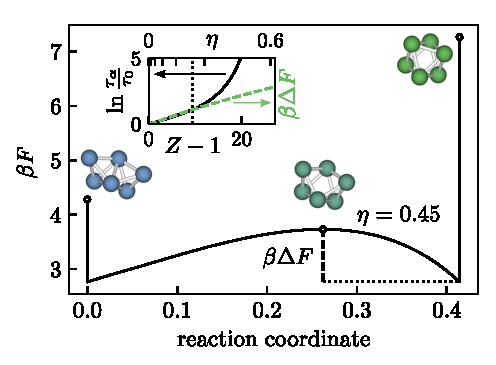
\includegraphics[width=0.9\linewidth,outer]{n6-reaction-path}
  \caption[The simplest nontrivial reaction path in hard spheres: octahedron to tripyramid]{
    Reaction for transition between tripyramid and octahedron $n = 6$ structures.
    Stationary points are indicated by markers: there is a discontinuity in free energy at the end points due to the additional integration over the reaction coordinate, and symmetry in the case of the octahedron.
    Inset: variation of activation barrier with volume fraction $\eta$ and compressibility $Z = \beta p/\rho$ from this theoretical reaction path (dashed line) and measured $\alpha$-relaxation times in bulk molecular dynamics simulations (solid line), where $\eta = 0.45$ is indicated with a vertical dotted line.
  }
  \label{fig:reaction-path-6}
\end{SCfigure}
\todo{Change compressibility factor to pressure}

\todo{Pictures of packings up to n7}

\section{Dynamics: free energy along a reaction path}

We have thus far focused on static thermodynamic properties: yet a connection with dynamics can be made by calculating the free energy along reaction paths between (geometrically similar) structures.
This calculation along unstable directions in the free energy landscape requires an analytic approach (described in the SM), and generates paths such as the one in Fig.\ \ref{fig:reaction-path-6}.
Here we consider transitions between the tripyramid and the octahedron with $n=6$ because this is the simplest nontrivial transition between distinct hard sphere packings (SM).
Comparing this dynamical barrier to the structural relaxation for ($\alpha$-) relaxation timescale $\tau_\alpha$ extracted from simulations relative to a microscopic time $\tau_0$ (inset of Fig.\ \ref{fig:reaction-path-6}), we find this single reaction path barrier agrees with the low density scaling of $\tau_\alpha$ (linear in the compressibility factor $\beta p / \rho$ \cite{BerthierPRE2009}).
However, activated dynamics are not expected in this regime so this agreement may be coincidental.
%Moving to high densities, hard spheres exhibit two-step relaxation when vibrational ($\beta$--) and full ($\alpha$--) relaxations decouple as the system approaches its glass transition \cite{Berthier2011}.
%However, dynamics along the tripyramid--octahedron path continues to increase in an ``Arrhenius'' fashion quite unlike the super-Arrhenius increase exhibited by the $\alpha$--relaxation in the computer simulations (inset of Fig.\ \ref{fig:reaction}).
%It has been shown in molecular systems that $\beta$--relaxation can be Arrhenius in the deeply supercooled regime where $\alpha$-- relaxation is super-Arrhenius \cite{Yu2015}.
%Given that typical particle displacements in the tripyramid--octahedron path are around 0.15$\sigma$ per particle, we observe that this relaxation mechanism may be more characteristic of ($\beta$--) relaxation than full ($\alpha$--) relaxation.
It is possible to extend our methodology for larger rearrangements, which may be sufficient to access ($\alpha$-) relaxation \emph{at very deep supercooling} for equilibrium systems.
However, the rapid growth in the number of possible states presents a considerable numerical challenge requiring new methods and approximations, so we leave this exciting avenue for future study.

\section{Conclusions}

We have presented a formalism for describing many-body correlations in liquids and developed it into an accurate and computationally efficient parameter-free theory for hard spheres using integral geometry relying solely on the choice of the equation of state.
The key approximations involved treating the grand potential as continuous and additive (related to extensivity), and imposing the correct contact value of $g^{(2)}(r)$.

We applied the framework to a selection of local structural correlations, therefore predicting nontrivial changes in the energy landscape with supercooling putting previous empirical observations on more solid ground.
In particular, our analysis provides evidence for the existence of two populations of structures with distinct symmetries and free energies which causes the local density of states to become increasingly bimodal at high densities.
We note that we have treated densities corresponding to a degree of supercooling only accessible using novel swap Monte Carlo techniques \cite{BerthierPRL2016}; however, these simulations introduce large polydispersity, changing the local structure \cite{CoslovichJPCM2018} and thus limiting direct comparison with our calculations for the monodisperse liquid.

Our framework can be easily adapted to more complex liquids such as systems with soft repulsive interactions and polydisperse mixtures \cite{KodamaJCP2011}.
Integral geometry underlies the core equation \eqref{eq:morphometric-surface-tension}, so this approach can extend to hard particles of more complex shapes where the interaction potential is still geometric in nature.
It is applicable to a more general class of liquids where the soft part of the potential may be treated as a perturbation around a hard core \cite{Hansen2013} such that a geometric decomposition still applies.
This suggests a new route for predicting static properties of equilibrium liquids, with direct applications to self-assembly, nucleation and protein structure.

\section{New notes.}

We wish to describe local structure.
Ultimately, we wish to learn about the structure of the energy landscape in hard spheres.
To do so we must characterise the main features of the landscape, namely the different geometric packings and assign weights (free energies) to them.
This is a worthy goal in its own right, perhaps not that interesting for hard spheres but useful for wider applications (e.g.\ predicting self assembly, guiding chemical synthesis, understanding protein folding kinetics and predicting the native state and design).

The path we take is as follows:
\begin{enumerate}
\item We need some means of weighting points in the energy landscape: we do this using the morphometric approach (cf previous chapter)
\item A means of characterising and approximating the entire phase space: energy landscape formalism (next). This has two subgoals:
  \begin{enumerate}
  \item Divide the landscape into stationary points: minima and saddles.
    These stationary points characterise submanifolds of the entire landscape, \emph{basins} in the case of minima and \emph{reaction paths} in the case of saddles.
  \item Integrate over connected manifolds with weight function (potential of mean force) to obtain their free energies.
  \end{enumerate}
\end{enumerate}

%Another way of saying this is we need an integrand and boundary conditions.

\subsection{Connection with energy landscape descriptions}

\begin{itemize}
  \item First describe the energy landscape description.
  \item Based on low-temperature expansion arguments.
  \item Mean-field: Laplace method/saddle-point.
  \item Gaussian expansion around this result (called Harmonic approximation in energy landscape/chemistry literature).
\end{itemize}

\begin{SCfigure}[H]
  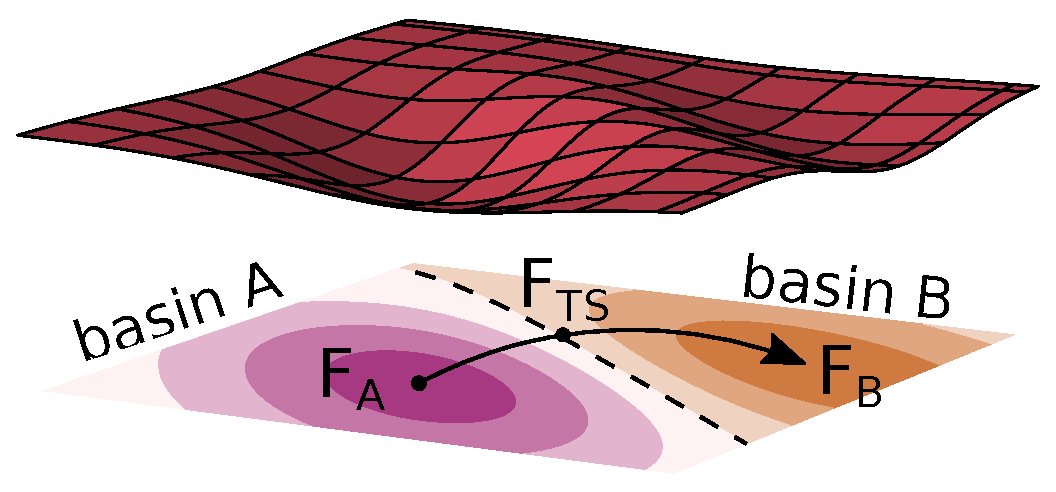
\includegraphics[width=\linewidth,outer]{toy-landscape}
  \caption[A cartoon energy landscape]{A cartoon energy landscape for a 2-dimensional phase space.
    The landscape features two local minima: $A$ and $B$.
    The area surrounding each minima defines its basin: any point from which the minima can be found by moving downhill belongs to the basin.
    Energy landscape approach: at low temperatures the system is expected to oscillate around potential energy minima, so the dynamics can be understood as rare events causing a change of basin.
    Thus a decomposition of the phase space in terms of basins should become exact for the dynamics at low temperatures in the supercooled regime of interest.}
\end{SCfigure}

In the case of local arrangements of hard spheres, rigid packings seem to correspond to minima of the potential of mean force.
I cannot prove this for the case of morphometric approach, but I cannot find a counter example.
Possibly can prove they are minimal volume.

\section{Locally favoured structures in hard spheres}

\subsection{Concentrations of local structure}

How do we define a local structure?
Most of the literature on structure in amorphous systems falls into one of either two categories
Almost all methods for Common methods:
\begin{itemize}
  \item Bond orientational order parameters
  \item Bond networks: take some bond detection algorithm (voronoi, 
Fom the partition function of the potential of mean force
Suppose we have a definition of a
\end{itemize}

From the definition of the probability density function in Eq.\ \eqref{eq:n-density-pdf}, the total number of local structures of a particular type in a volume $V$ is
\begin{equation}\label{eq:structure-population}
  \mathcal{N} =
  \int_{\mathcal{Q}} \rho^n g^{(n)}(\vec{r}^n) \, d\vec{r}^n,
\end{equation}
where $\mathcal{Q}$ is the domain \emph{defining} the local structure.
To get the free energy expression used in the main text we consider the manifold diffeomorphic to translations, defining $\mathcal{Q} = \mathcal{D} \rtimes \mathbb{V}$ where $\mathbb{V}\subset \mathbb{R}^3$ is the system volume.
Exploiting translational invariance of the potential of mean force, we fix one particle at the origin and integrate the center of mass over the system volume giving
\begin{equation}
  \mathcal{N} =
  \rho^n V \int_{\mathcal{D}} g^{(n)}(\vec{r}^n) \, d\vec{r}^{n-1}.
\end{equation}
We defined a free energy by taking $\mathcal{N} = \sigma^{3(n-1)} \rho^n V e^{-\beta F}$, which together with the above expression gives Eq.\ \eqref{eq:local-structure-free-energy} in the main text.

More generally, we consider the manifold diffeomorphic to translations \emph{and} rotations.
We define $\mathcal{Q} = \mathcal{D}' \rtimes SE(3)$ where $\textrm{SE}(d)$ is the $d$-dimensional special Euclidean group, leaving the $\mathcal{D}'$ as the space of the structure's internal motion.
\todo{Make this consistent with the notation of background chapter.}
We separate rigid body from internal motion by applying the following transformation to each particle coordinate
\begin{equation}
  \vec{r}(\{\vec{t}, \vec{\theta}, \vec{x}\}) =
  \vec{t} + \vec{R}(\vec{\theta}) \cdot \vec{q}(\vec{x}),
\end{equation}
where $\vec{t}$ is the translation vector, $\vec{\theta}$ the Euler angles, $\vec{R}$ the rotation matrix, and $\vec{x} \in \mathbb{R}^{3n-6}$ represents the internal coordinates.
We need to compute the metric of this transformation $G_{ij} = \vec{G}_i \vec{G}_i^T$ where the (generally curvilinear) basis vectors are $\vec{G}_i = \partial_i \vec{r}$.
To simplify calculation we choose $\vec{q}(\vec{x})$ to always be in the center-of-mass frame and orthogonal to rotations such that $G_{ij}$ reduces to block-diagonal form.
If the rotation matrix is expressed in Euler-angle representation as $\vec{R}(\vec{\theta}) = \vec{R}_3(\theta_3) \vec{R}_2(\theta_2) \vec{R}_1(\theta_1)$ then we have%
\marginfootnote{There is no elegent omitted step to obtain the form of $\vec{U}$ which gives the block diagonal form; rather, I used a series of educated guesswork within Mathematica to obtain this.
  There is probably a more direct route.}
\begin{equation}
  \vec{G}(\vec{\theta}, \vec{x}) =
  \begin{pmatrix}
    n \vec{E} & 0 & 0 \\
    0 & \vec{U}^T(\vec{\theta}) \vec{I}(\vec{x}) \vec{U}(\vec{\theta}) & 0 \\
    0 & 0 & \overline{\vec{G}}(\vec{x})
  \end{pmatrix},
\end{equation}
where $\vec{E}$ is the identity matrix, $\overline{\vec{G}}$ is the metric for internal motion, and we have defined the matrix $\vec{U}$ as
\begin{equation}
  \vec{U}(\vec{\theta}) =
  \begin{pmatrix}
    1 &  0              & -\sin{\theta_2} \\
    0 &  \cos{\theta_1} &  \cos{\theta_2} \sin{\theta_1} \\
    0 & -\sin{\theta_1} &  \cos{\theta_2} \cos{\theta_1} \\
  \end{pmatrix}
  \qquad
  \begin{aligned}
    \theta_1 &\in [0,2\pi] \\
    \theta_2 &\in \left[-\frac{\pi}{2},\frac{\pi}{2}\right] \\
    \theta_3 &\in [0,2\pi].
  \end{aligned}
\end{equation}
Note $\det{\vec{U}} = \cos{\theta_2}$.
The volume element in the new coordinates is
\begin{equation}
  d\vec{r}^n = \frac{\sqrt{\det G_{ij}(\vec{x})}}{\nu}
  \, d^3 \vec{t} \, d^3 \vec{\theta} \, d^{3n-6} \vec{x},
\end{equation}
where $\nu$ is the symmetry number (discussed below) and
\begin{equation}
  \sqrt{\det G_{ij}(\vec{x})} =
  \cos{\theta_2} \sqrt{\det{\vec{I}(\vec{x})}}
  \sqrt{n^3 \det{\overline{G_{ij}}(\vec{x})}}.
\end{equation}
The symmetry number emerges as the choice of internal coordinates typically fixes the particle labels breaking permutation symmetry; we have to multiply by the $n!$ possible labellings, which introduces double counting if the structure possesses rotational symmetry so we have to divide by the correcting factor $\nu$.
This is explained in detail in Ref.\ \cite{CatesSM2015}.
Thus \eqref{eq:structure-population} reduces to
\begin{equation}\label{eq:structural-partition-function-detailed}
  \frac{\mathcal{N}}{\rho^n V}
  =
  \frac{8\pi^2 \sqrt{n^3}}{\nu} \int_{D'}
  g^{(n)}(\vec{x}) \,
  \sqrt{\det{\overline{G_{ij}}(\vec{x})} \det{\vec{I}(\vec{x})}}
  \, d^{3n-6} \vec{x}.
\end{equation}
Note that in the limit of linear molecules, i.e.\ where all particles fall on a line, the above approach fails as there is one less rotation mode requiring a modified description.

In general, the integrand in \eqref{eq:structural-partition-function-detailed} is only exactly solvable for the simplest geometries due to the high dimensionality of $\vec{x}$.
This is further complicated by the fact that the basis vectors for $\overline{G_{ij}}$ are curvilinear.
We use two methods for evaluating these integrands:
\begin{enumerate}
\item Monte Carlo simulation: described in the next section.
\item Analytically via perturbation theory: described in sections \ref{SI:bond-distance} and \ref{SI:reaction-path}.
  We use this for a similar integrand along a reaction path where Monte-Carlo cannot be used directly.
\end{enumerate}

\subsection{Bond-distance space}
To evaluate the integrand in Eq.\ \eqref{eq:structural-partition-function-detailed} analytically we need to choose a representation for $\vec{x}$ which is diffeomorphic to $\vec{r}^n$.
For \emph{minimally constrained geometries}, i.e.\ structures with exactly $3n-6$ contacts, a convenient representation exists: bond distance space.
Following Ref.\ \cite{Holmes-CerfonPNAS2013} and its accompanying Supplementary Information we choose each element of $\vec{x}$ to represent the distances between particles in contact, where contact occurs at $\vec{x} = (\sigma, \dots, \sigma)$.
Thus increasing elements of $\vec{x}$ corresponds to thermal fluctuations away from contact.
This representation naturally expresses the limits of integration given in the main text as $\sigma \le x_i \le \sigma_{cut}$.

To evaluate the integral we need expressions for the internal metric and moment of inertia terms.
The internal metric is defined in terms of the Jacobian matrix $\vec{J} \in \mathbb{R}^{3n \times 3n-6}$
\begin{equation}
  \overline{G_{ij}} = \vec{J}^T \vec{J}
\end{equation}
where the matrix entries are given by
\begin{equation}
  J_{ij} = \frac{\partial q_i}{\partial y_j}.
\end{equation}
In practice it is easier to calculate its inverse numerically (via finite differences) using
\begin{equation}
  J_{ij}^{-1}
  = \frac{\partial y_j}{\partial q_i}
  = \left. \frac{\partial y_j}{\partial x_i}
  \right|_{\vec{\theta} = \vec{t} = \vec{0}}
\end{equation}
which has linearly independent rows for a minimally constrained geometry so we recover $\vec{J}$ from $\vec{K} = \vec{J}^{-1}$ using the matrix inversion formula $\vec{J} = (\vec{K}^T\vec{K})^{-1} \vec{K}^T$.
The above expressions all depend implicitly on the point $\vec{x}$ as the coordinate scheme is curvilinear, so to keep the integral tractable we approximate this to leading order as
\begin{equation}
  \sqrt{\overline{G_{ij}}(\vec{x})} \simeq \sqrt{\overline{G_{ij}}(\vec{x}_0)}
\end{equation}
where $\vec{x}_0 = (\sigma,\dots,\sigma)$ is contact.
Thus the integral becomes
\begin{equation}\label{eq:structural-partition-function-approximated}
  \frac{\mathcal{N}}{\rho^n V}
  =
  \frac{8\pi^2 G_0}{\nu} \int_{D'}
  g^{(n)}(\vec{x}) \,
  \sqrt{\det{\vec{I}(\vec{x})}}
  \, d^{3n-6} \vec{x}
\end{equation}
where $G_0 = \sqrt{n^3 \det{\overline{G_{ij}}(\vec{x}_0)}}$.

Finally, we write the distribution function in terms of the potential of mean force and expand this and the moment of inertia to first order, as in
\begin{align}
  \phi^{(n)}(\vec{x}) &=
  \phi^{(n)}(\vec{x}_0) +
  (\vec{x} - \vec{x}_0) \cdot
  \left. \vec{\nabla} \phi^{(n)}(\vec{x}) \right|_{\vec{x} = \vec{x}_0} +
  \mathcal{O}(\vec{x}^2), \\
  \sqrt{\det{\vec{I}(\vec{x})}} &=
  \sqrt{\det{\vec{I}(\vec{x}_0)}} +
  (\vec{x} - \vec{x}_0) \cdot
  \left. \vec{\nabla} \sqrt{\det{\vec{I}(\vec{x})}} \right|_{\vec{x} = \vec{x}_0} +
  \mathcal{O}(\vec{x}^2).
\end{align}
Using the analytical gradient expressions given in Section \ref{SI:line-curvature} makes this calculation very efficient.
The integral \eqref{eq:structural-partition-function-approximated} separates into $3n-6$ independent one-dimensional integrals of the form
\begin{equation*}
  \int_\sigma^{\sigma_{cut}} (a_i + b_i x_i) e^{-c_i x_i} dx_i
  = \left[
    - \left(
    \frac{(a + b_i x_i)}{c_i} + \frac{b_i}{c_i^2} \right) e^{-c_i x_i}
  \right]_\sigma^{\sigma_{cut}},
\end{equation*}
where $a_i$, $b_i$ and $c_i$ are constants.

Loosely speaking, this is the hard-particle analogue of the harmonic approximation with the difference here being that the first derivative does not vanish at the minimum.
For $n=6$ this expansion works rather well, as all structures have exactly $3n-6$ bonds and this perturbation theory captures the free energy well when compared with the ``exact'' result from thermodynamic integration.

\section{Introduction}

This study builds on and contributes to work in nonequilibrium statistical physics, particularly relating to glasses and nucleation.
Although small-system studies have examined how dynamics are influenced by topographical properties of the energy landscape for simple systems, there has not been a systematic formalism for extending this to the bulk liquid.
As such, this study provides additional insight into dynamical arrest i.e.\ the supercooled liquid and glasses.

The analytic focus on many-body correlations provides another contribution to the fundamental understanding of simple liquids.
This study analyses depletion forces in order to predict the many-body correlation functions in the bulk liquid.
Although numerous studies have identified the role of local structure in dynamical arrest little analytical attention has been paid to how to properly formulate structure in a quantitative thermodynamic framework.
I address this issue by expressing the solvation free energies in terms of geometrical properties of a small solute, and develop techniques for making quantitative predictions of local structure in the hard sphere liquid.

Energy landscape can be divided into two strands: the topographic view of Stillinger which offers a powerful conceptual tool for understanding complex phenomena.
At low temperatures we can imagine the system oscillating around low energy minima (inherent states), with occasional large fluctuations driving it through `choke points' causing a change to a different energy minimum.
This formalism was turned into a properly quantitative framework by Wales \cite{Wales2004,?}, where stationary point databases are constructed: energy minima connected by saddles.
From the connectivity of the landscape one can understand dynamical arrest: if there are lots of competing low lying minima it can be hard for the system to find the global minimum and we expect it to fall out of equilibrium easily when temperature is lowered.
By contrast, if the minima steadily lower in energy then they act as a funnel to the global minimum so we expect rapid equilibration.

Quantitative predictions are typically only possible for small systems, so it is desirable to extend it to the bulk.
One can to do this focusing on a subset of the total degrees of freedom, integrating out the rest in an approximate fashion.
The selected degrees of freedom act as a small system with a many-body interaction potential, so can be treated with the aforementioned formalism in a quantitative manner.
This was attempted by Tarjus \cite{?} with mixed success.
The morphometric approach \cite{KonigPRL2004,RothPRL2006,RobinsonPRL2019} offers a generic framework to treat many-body correlations allowing a first-principles treatment of local structure in the bulk liquid.
This framework is accurate for hard spheres where it has been extensively tested \cite{Hansen-Goos?,Roth?,Bob?,RobinsonPRL2019}.

Hard particle systems are the fundamental system of interest for simple liquids.
The stationary point database approach, firmly rooted in \emph{potential energy}, fails for hard systems as the potential energy is trivial so the thermodynamics is athermal.
It has never been extended to hard systems until now.
This extension comes with the cost that some of the elegant techniques of soft systems will fail due to the singular nature of hard sphere interactions, so we require new methods to handle the idiosyncrasies of hard systems.
Here we propose a practical definition for basins when working with hard systems, and develop techniques for evaluating thermodynamic quantities with this definition.
We then retroactively justify the meaningfulness of this basins by comparing with simulation/literature data.

\todo{Talk about the past work on hard spheres: penny packing, and sticky spheres.}
A number of unique technical challenges brought about by the hard sphere potential, that we will solve.
The groundwork for this was laid down by Holmes-Cerfon and coworkers.
Note: attempts have been successful at modelling effective interactions close to isostaticity where $z \to 2d$.
This is empirically found to be the case asymptotically as one approaches jamming, however it is worth noting that there is no general requirement that $z = 2d$ for rigid packings, and counter examples where $z < 2d$ are known.

In section \ref{sec:energy-landscapes} we review the energy landscape formalism for soft potentials, with a view to highlighting where it might fail for hard interactions.
We review the liquid state theory/morphological approach used for treating the depletion interactions between hard particles in the bulk liquid in section \ref{?},
followed by the equivalent of the partition function for local structure.
Our core theoertical results are then presented in section \ref{?}, where we propose a definition of local structure and show techniques for evaluating the partition function nonperturbatively.
We then present the results of the topography of the local structural energy landscape in hard spheres in section \ref{?}, our main numerical results.

\section{Energy landscape approaches}
\label{sec:energy-landscapes}

Points to cover:
\begin{itemize}
\item Give a technical definition of local structure with a goal to showing the problems with hard systems.
\item Define structures as manifold: $\mathbb{R}^{dn}$ for $n \ll N$, embedded in $\mathbb{R}^{dN}$
\item Failure of perturbation theory due to singularity of 
\end{itemize}

The energy landscape/inherent structure approach is a powerful theoretical framework for understanding complex phenomena.
At its core, it is a means of coarse-graining the high dimensional phase space into a more manageable mesostates.
Its power comes from the fact that it is essentially exact, though calculations are typically intractable unless the degrees of freedom can be significantly reduced; in practice this is generally only possible in mean field (high spatial dimensions) or for small systems $N = \mathcal{O}(10)$ in physical settings.
The approach is however useful conceptually for developing theories based around the topography of the energy landscape \cite{Stillinger}, and makes detailed calculations tractable typically for small systems \cite{Wales2004}.

In this section we will review the energy landscape approach, how it applies to soft potentials and the complications that arise for our system of interest: hard spheres.
First we talk about coarse-graining into mesostates mentioned above, whether into inherent structures or otherwise.
A mesostate is a collection of microstates which are grouped together, typically these are selected for sharing some desirable property to simplify description.
For practical reasons this means that microstates should be connected in phase space so they are compact manifolds.
In connection with the topographic view we will call these manifolds \emph{basins}.
The total partition function is then decomposed as
\begin{equation}
  Z \equiv \int_{\mathbb{R}^{dN}} e^{-\beta (U_N(\vec{r}^n) + \phi(\vec{r}^n))} \, d\vec{r}^N = \sum_i Z_i
\end{equation}
where $\phi$ is the external potential of the container in order to keep the particles localised in a region where they interact.
Alternatively they could be embedded in a toroidal topology to prevent particle dissociation (as in e.g.\ simulations with periodic boundary conditions).
The basin partition function is
\begin{equation}
  Z_i = \int_{\mathbb{V}_i^{dN}} e^{-\beta U_N(\vec{r}^N)} \, d\vec{r}^N
\end{equation}
if $\mathbb{V}_i^{dN} \subset \mathbb{R}^{dN}$ is the manifold corresponding to basin $i$.
One can define (e.g.\ Wales).
Despite a definition which unambiguously demarcates the basins, the high dimensionality of the phase space renders the integrals in \eqref{eq:basin-partition-function} completely intractable without approximation.

The equilbrium probability of the system being in basin $i$ at any one time is thus
\begin{equation}
  p_i = \frac{Z_i}{Z}
\end{equation}
From the Gibbs-Shannon entropy we find the coarse-graining entropy
\begin{equation}
  \begin{split}
    S_{\textrm{conf}}
    &= -\sum_i p_i \ln{p_i} \\
    &= -\sum_i \left( \frac{Z_i}{Z} \ln{Z_i} - \frac{Z_i}{Z} \ln{Z} \right) \\
    &= \ln{Z} - \sum_i \frac{Z_i}{Z} \ln{Z_i}
  \end{split}
\end{equation}
Noting that the total free energy is $F = -k_B T \ln{Z}$ we thus have
\begin{equation}
  \beta F = \langle \beta F_i \rangle - S_{\textrm{conf}}
\end{equation}
where the average basin free energy $F_i = -k_B T \ln{Z_i}$ is
\begin{equation}
  \langle \beta F_i \rangle = - \frac{1}{Z} \sum_i Z_i \ln{Z_i}
\end{equation}

Finally, we have to choose how to define the basins.
In the energy landscape approach the coarse-graining occurs around local minima of energy where $\vec{\nabla}U_N = 0$ and Hessian $\frac{1}{2}\vec{\nabla}\vec{\nabla}U_N$ is positive definite.
Each basin consists of all the points connected by a steepest descent path to a unique energy minimum.
This description reduces the high dimensional continuous description down to discrete number of zero-dimensional manifolds.
In practice the number of minima scales exponentially in $N$, so this is still an intractably large number of points.
One can even obtain dynamical information by considering the saddles, i.e.\ the unstable stationary points.
The saddles act as the lowest (in energy) lying points that must be crossed to jump from one basin to another, giving the energy barriers to dynamics.

How do we justify this approach?
Energy is smooth so asymptotics around stationary points is valid: inherent state (stable stationary points) description
For infinite systems we could use Laplace method
\begin{equation}
  \int_{\mathbb{V}^{dN}_i} e^{-\beta N u_N(\vec{r}^N)} \, d\vec{r}^N
  \sim
  e^{-\beta \min{U_N(\vec{r}^N)}} \qquad \forall \; N \gg 1
\end{equation}
where $u_N = U_N / N$.
For finite systems we could go beyond this pertubatively by employing a harmonic approximation from the energy-landscape literature
\begin{equation}
  U_N = U_N(\vec{p}_i) +
  \frac{1}{2} \Delta \vec{r} \cdot \left. \nabla \nabla U_N\right|_{\vec{p}_i} \cdot \Delta \vec{r}
  + \mathcal{O}(\Delta \vec{r}^3)
\end{equation}
where \[\vec{p}_i = \argmin_{\vec{r}^n \in \mathbb{V}_i^{dN}}{\left(U_N(\vec{r}^n)\right)}\] is the location of the energy minimum.
\begin{equation}
  Z_i \sim \exp{-\beta U_N(\vec{p}_i)}
\end{equation}
There are two layers of approximation: first we model the pdf as a Gaussian, second we approximate the boundary conditions as being infinite.
The inclusion of the Hessian term in the expansion around the minimum shows that for soft potentials one can perturbatively build a description around the inherent states.
At low temperatures this approach is expected to become exact (for the first layer not the second one).
So for athermal systems perturbation theory should break down.

\begin{SCfigure}
  \missingfigure[figwidth=\linewidth]{}
  \caption{Failure of Laplace method for hard interactions.}
\end{SCfigure}

To make the above discussion concrete we will consider two examples.
First, we examine a symmetric quartic potential
\begin{equation}
  \phi = \epsilon (x^4 - x^2)
\end{equation}
where $x$ is some state variable and $\epsilon$ is an energy scale.
This could represent e.g.\ a ferromagnet below the critical temperature with $x$ representing the spontaneous magnetisation.
The free energy in units of $\epsilon$ is then
\begin{equation}
  F = - T \ln{\left( \int \exp{\left(-\frac{\phi}{T}\right)} \, dx \right)}
\end{equation}
This potential naturally contains two basins for the two half space $x \in [-\infty, 0]$ and $x \in [0, \infty]$, and because of the symmetry of the potential around $x=0$ the contribution of each of these basins is identical, i.e.\
\begin{equation}
  Z = 2 \int_0^\infty \exp{\left(-\frac{\phi}{T}\right)} \, dx.
\end{equation}
Applying the harmonic approximation
\begin{equation}
  \begin{split}
  Z &\simeq
  2 \exp{\left( -\frac{\phi(x_0)}{T} \right)}
  \int_{-\infty}^\infty \exp{\left(-\frac{\phi''(x_0)}{2T}\right)} \, dx \\
  &=
  2 \exp{\left( -\frac{\phi(x_0)}{T} \right)}
  \sqrt{\frac{2 \pi T}{\phi''(x_0)}}
  %+ \mathcal{O}(\phi'''(x_0))
  \end{split}
\end{equation}
where $x_0 = \dfrac{1}{\sqrt{2}}$ is the position of the minimum in the $x > 0$ basin.

The hard sphere potential is a pathological case: the singularity in the pair potential dooms harmonic treatments.
To illustrate this, we consider a worked example.
Consider as a worked example two one-dimensional particles interacting via a repulsive inverse power law $u_{\textrm{pair}}(r) = \epsilon r^{-\gamma}$ for $\gamma > 1$ where $\epsilon > 0$ is the interaction energy, and depletion interactions modelled as a linear term $u_{\textrm{depletion}}(r) = r$.
This toy model approximately corresponds to the small $r$ behaviour close to contact for 3d hard spheres Fig.\ \ref{?}.
The partition function is
\begin{equation}
  %\begin{split}
  Z(\gamma)
  = \int_1^{\infty} \exp{\left(-\frac{\epsilon}{r^\gamma}\right)} \, dr
  = \left[ \frac{r^{1-\gamma}}{1-\gamma} \right]_1^\infty
  = \frac{1}{\gamma - 1}
  %\end{split}
\end{equation}
The free energy is thus
\begin{equation}
  F(\gamma) = \ln{(\gamma - 1)}
\end{equation}
which is a finite quantity for all $r$.
If we compare this against the harmonic approximation, however, we obtain
\begin{equation}
  F(\gamma) \propto \gamma(\gamma - 1)
\end{equation}
which diverges in the hard sphere limit $\gamma \to \infty$.
The hard sphere limit is properly singular, and we must use nonperturbative methods to treat it.
We will however take inspiration of the approach for soft potentials, and hope to adapt these into a framework for doing similar calculations.

To summarise this section, we note that the basin definition of structures for soft potentials has the properties that: \cite{Wales?}
\begin{itemize}
\item Each basin $B_i$ connects to a unique minimal energy state with a unique geometry.
\item Divide the phase space into basins which do not overlap $B_i \cap B_j = \emptyset$ for $i \ne j$ and tile the whole of phase space $\cup_i B_i = \mathbb{R}^q$.
\item Its free energy is well-defined (at least in some asymptotic limit) so it can be approximated with simple methods.
  For soft potentials this is a consequence of the first criterion.
  This makes the choice of coarse-graining (thermo)dynamically meaningful: it is long-lived enough that the microstates making up a basin can be not distinguished, and the dynamics reduces to basin crossing events.
\end{itemize}
A definition satisfying the first two criteria is possible, however due to the singularity in the hard particle interaction potential the region surrounding the (depletion) energy minimum is thermodynamically irrelevant.
This can be interpretted:
\begin{itemize}
\item \emph{Thermodynamically}: the region near contact is entropically suppressed, regions away from contact have many more microstates so are entropically enhanced
\item \emph{Dynamically}: as hard spheres approach one another they collide and bounce away so spend infinitesimally small timescales at contact.
  Collisions almost universally involve only two particles, collisions of more than two particles occur with zero measure.
\end{itemize}
Because of this we cannot obtain the free energy by a small parameter expansion around the contact point.
We must evaluate the full integral over a finite volume.
To make this tractable we will abandon the rigorous definition of structures in terms of basins employed for soft potentials, in favour of a simple one based on intuitive geometrical ideas.
We will later explore the limitations/successes of this definition in order to retroactively justify this approach.

Due to the analogies between the population/concentration integral and the usual partition function, we will refer to this integral simply as a partition function.

\subsection{Molecular partition function}

From the definition of the probability density function in Eq.\ \eqref{eq:n-density-pdf}, the total number of local structures of a particular type in a volume $V$ is
\begin{equation}\label{eq:structure-population}
  \mathcal{N} =
  \int_{\mathcal{Q}} \rho^n g^{(n)}(\vec{r}^n) \, d\vec{r}^n,
\end{equation}
where $\mathcal{Q}$ is the domain \emph{defining} the local structure.
To get the free energy expression used in the main text we consider the manifold diffeomorphic to translations, defining $\mathcal{Q} = \mathcal{D} \rtimes \mathbb{V}$ where $\mathbb{V}\subset \mathbb{R}^3$ is the system volume.
Exploiting translational invariance of the potential of mean force, we fix one particle at the origin and integrate the center of mass over the system volume giving
\begin{equation}
  \mathcal{N} =
  \rho^n V \int_{\mathcal{D}} g^{(n)}(\vec{r}^n) \, d\vec{r}^{n-1}.
\end{equation}
We defined a free energy by taking $\mathcal{N} = \sigma^{3(n-1)} \rho^n V e^{-\beta F}$, which together with the above expression gives Eq.\ \eqref{eq:local-structure-free-energy} in the main text.

There will be $d$ translation modes and $\frac{d(d-1)}{2}$ rotational modes for each plane formed by pairs of coordinate axes (e.g.\ $x^1 \wedge x^2$ for rotations in the $x^1x^2$-plane).
Subtracting the number of rigid body modes from the total degrees of freedom gives \[ q = dn - \frac{d(d+1)}{2} \] internal degrees of freedom.
Exception when rotations are degenerate: $n < d$ (e.g.\ $n=2$ in $d=3$) or pathological cases of unusually high symmetry (e.g.\ when all particles fall on a line) which can in general be excluded.

More generally, we consider the manifold diffeomorphic to translations \emph{and} rotations.
We define $\mathcal{Q} = \mathcal{D}' \rtimes SE(3)$ where $\textrm{SE}(d)$ is the $d$-dimensional special Euclidean group, leaving the $\mathcal{D}'$ as the space of the structure's internal motion.
We separate rigid body from internal motion by applying the following transformation to each particle coordinate
\begin{equation}
  \vec{r}(\{\vec{t}, \vec{\theta}, \vec{x}\}) =
  \vec{t} + \vec{R}(\vec{\theta}) \cdot \vec{q}(\vec{x}),
\end{equation}
where $\vec{t}$ is the translation vector, $\vec{\theta}$ the Euler angles, $\vec{R}$ the rotation matrix, and $\vec{x} \in \mathbb{R}^{3n-6}$ represents the internal coordinates.
We need to compute the metric of this transformation $G_{ij} = \vec{G}_i \vec{G}_i^T$ where the (generally curvilinear) basis vectors are $\vec{G}_i = \partial_i \vec{r}$.
To simplify calculation we choose $\vec{q}(\vec{x})$ to always be in the center-of-mass frame and orthogonal to rotations such that $G_{ij}$ reduces to block-diagonal form.
If the rotation matrix is expressed in Euler-angle representation as $\vec{R}(\vec{\theta}) = \vec{R}_3(\theta_3) \vec{R}_2(\theta_2) \vec{R}_1(\theta_1)$ then we have%
\footnote{While the final form of $\vec{G}$ is elegant, I do not have a straightforward way of getting it; it involved a lot of guesswork and within Mathematica to find a form of $\vec{U}$ which gives the middle block.
  There is probably a more direct route.}
\begin{equation}
  G_{ij}(\{\theta_i\}, \vec{x}) =
  \begin{pmatrix}
    n \vec{E} & 0 & 0 \\
    0 & \vec{U}^T(\vec{\theta}) \vec{M}(\vec{x}) \vec{U}(\vec{\theta}) & 0 \\
    0 & 0 & \overline{G_{ij}}(\vec{x})
  \end{pmatrix},
\end{equation}
where $\vec{E}$ is the identity matrix, $\vec{M}$ is the moment of inertia tensor, $\overline{G_{ij}}$ is the metric for internal motion, and we have defined the matrix $\vec{U}$ as
\begin{equation}
  \vec{U}(\vec{\theta}) =
  \begin{pmatrix}
    1 &  0              & -\sin{\theta_2} \\
    0 &  \cos{\theta_1} &  \cos{\theta_2} \sin{\theta_1} \\
    0 & -\sin{\theta_1} &  \cos{\theta_2} \cos{\theta_1} \\
  \end{pmatrix}
  \qquad
  \begin{aligned}
    \theta_1 &\in [0,2\pi] \\
    \theta_2 &\in \left[-\frac{\pi}{2},\frac{\pi}{2}\right] \\
    \theta_3 &\in [0,2\pi].
  \end{aligned}
\end{equation}
Note $\det{\vec{U}} = \cos{\theta_2}$.
The volume element in the new coordinates is
\begin{equation}
  d\vec{r}^n = \frac{\sqrt{\det G_{ij}(\vec{x})}}{\nu}
  \, d^3 \vec{t} \, d^3 \vec{\theta} \, d^{3n-6} \vec{x},
\end{equation}
where $\nu$ is the symmetry number (discussed below) and
\begin{equation}
  \sqrt{\det G_{ij}(\vec{x})} =
  \cos{\theta_2} \sqrt{\det{\vec{M}(\vec{x})}}
  \sqrt{n^3 \det{\overline{G_{ij}}(\vec{x})}}.
\end{equation}
The symmetry number emerges as the choice of internal coordinates typically fixes the particle labels breaking permutation symmetry; we have to multiply by the $n!$ possible labellings, which introduces double counting if the structure possesses rotational symmetry so we have to divide by the correcting factor $\nu$.
This is explained in detail in Ref.\ \cite{CatesSM2015}.
Thus \eqref{eq:structure-population} reduces to
\begin{equation}\label{eq:structural-partition-function-detailed}
  \frac{\mathcal{N}}{\rho^n V}
  =
  \frac{8\pi^2 \sqrt{n^3}}{\nu} \int_{D'}
  g^{(n)}(\vec{x}) \,
  \sqrt{\det{\overline{G_{ij}}(\vec{x})} \det{\vec{M}(\vec{x})}}
  \, d^{3n-6} \vec{x}.
\end{equation}
Note that in the limit of linear molecules, i.e.\ where all particles fall on a line, the above approach fails as there is one less rotation mode requiring a modified description.

Note that for all of the geometries we have tested this metric seems to be 2, although we could not prove this is in the general case.
We have to actually evaluate the integral.
We will explore thermodynamic integration using Monte Carlo, which is essentially exact to numerical precision but slow, and some analytical approximations.

\subsection{Worked examples}

%% \begin{SCfigure}
%%   \missingfigure[figwidth=\linewidth]{}
%%   \caption{Number of first shell neighbours in the hard sphere liquid.}
%% \end{SCfigure}

%% \begin{SCfigure}
%%   \missingfigure[figwidth=\linewidth]{}
%%   \caption{Number of equilateral triangles in the hard sphere liquid.}
%% \end{SCfigure}

We will consider two worked examples for simple geometries which are readily visualised and for which the metric $G(\vec{x})$ is known exactly and the partition function integral reduces to a simple form.

Our first worked example is at the two-body level: the typical number of neighbours in the first shell.
For a dimer the metric term evaluates to $G(\vec{x}) = r^2$, i.e.\ the usual spherical coordinate Jacobian as expected.
The average number neighbours less than some distance $r$ is then
\begin{equation}
  z(r)
  = 4\pi \int_0^r g^{(2)}(r) r^2 \, dr
  = 4\pi \int_\sigma^r e^{-\beta \phi^{(2)}(r)} r^2 \, dr
\end{equation}
This is a common measurement where $r$ is taken up to the first minimum of the $g(r)$ then $z$ corresponds to the number in the ``first-shell'' (i.e. the coordination number).

Our second worked example considers the average concentration of triangles in the liquid.
Here the relevant coordinates are the tuple $\vec{x} = (r,s,t)$ where the three distances are the lengths of the triangle.
The metric has previously been determined exactly as $G(\vec{x}) = rst$ in \cite{?}.
The number of equilateral triangles with maximum side length $\delta$ is then
\begin{equation}
  N_\Delta(\delta)
  =
  8\pi^2 \int_\sigma^\delta\int_\sigma^\delta\int_\sigma^\delta
  e^{-\beta\phi^{(3)}(r,s,t)} rst \, dr ds dt.
\end{equation}
The results show excellent agreement with molecular dynamics simulations across the entire liquid regime, and even into the supercooled regime where simulations are available for a polydisperse system.

\subsection{Exact result: thermodynamic integration}

\todo{State that we want the saddles: they are the primary reason for developing analytical methods}

Before moving on to our approximate analytical integration schemes we describe a method which is essentially exact to within numerical precision, at the cost of greater computational expense.
We will use thermodynamic integration to test the accuracy of our analytical methods.
Aspects of this method were inspired by Ref.\ \cite{SchillingJCP2009}.
As a Monte-Carlo method it would be very difficult to extend this method to saddles which is of great interest.

We perform a thermodynamic integration between two potentials $V_1$ and $V_2$ by considering the intermediate potential
\begin{equation}
  V(\vec{r}^n; V_1, V_2) = \lambda V_1(\vec{r}^n) + (1-\lambda) V_2(\vec{r}^n).
\end{equation}
where $\lambda \in \{0,1\}$ is a mixing parameter.
Over the course of a Monte-Carlo sweep, in addition to regular steps $\lambda$ is allowed to switch between these values according to the Metropolis-Hastings rule.
The free energy difference between the two systems is determined from the ratio of time spent with each potential active by
\begin{equation}
  \Delta F \equiv F_2 - F_1 = -\log{\left( \frac{t_2}{t_1} \right)},
\end{equation}
where $t_i$ is the total number of sweeps where potential $i$ is active (by $\lambda$ value).

Local structure is defined in the main text by its bond topology.
We define an $n \times n$ adjacency matrix $\mathcal{A}$ giving the bond topology of $n$ particles by
\begin{equation}
  A_{ij} =
  \begin{cases}
  1 \quad i \textrm{ and } j \textrm{ ``bonded''} \\
  0 \quad \textrm{otherwise}
  \end{cases}
\end{equation}
The hard core interaction ensures $r_{ij} \equiv |\vec{r}_i - \vec{r}_j| > \sigma$ for all $(i,j)$ including non-bonded particles, but the ``bonded'' flag forces the stricter condition that $r_{ij} \in [\sigma, \sigma_{cut}]$ when $A_{ij} = 1$.
The latter strict criterion is how we are able to focus on specific local structures.

To do the thermodynamic integration we introduce an intermediate potential which takes into account the boundary conditions of the integral:
\begin{equation}
  \phi(\vec{r}^n; v_\lambda, \eta) =
  \sum_{i < j} A_{ij} v_\lambda(r_{ij})
  + \phi^{(n)}(\vec{r}^n; \eta)
\end{equation}
where $v_\lambda$ is a \emph{confining} potential to restrict the Monte-Carlo to integrate only the structure of interest.
We have indicated the dependence of the potential of mean force on volume fraction, noting that in the ideal gas limit the grand potential (solvation) term vanishes leaving only the potential energy contribution
\begin{equation}
  \phi^{(n)}(\vec{r}^n; \eta=0) = \sum_{i < j} v_{hs}(r_{ij}),
\end{equation}
where the hard sphere (no-overlap) interaction is
\begin{equation}
  v_{hs}(r) =
  \begin{cases}
    0 &r > \sigma \\
    \infty &\textrm{elsewhere}.
  \end{cases}
\end{equation}
The potential of interest is $\phi(\vec{r}^n; v_{hs}, \eta)$, which requires several thermodynamic integration steps to reach.

First, we perform an integration from a reference potential $\phi(\vec{r}^n; v_H, \eta=0)$ to $\phi(\vec{r}^n; v_{SW}, \eta=0)$ where the confining potential $v_\lambda$ takes either the harmonic form
\begin{equation}
  v_H(r) = \epsilon \left(\frac{\sigma_{cut} - r}{\sigma}\right)^2
\end{equation}
with a value of $\epsilon$ discussed below, or the (infinite) square well form
\begin{equation}
  v_{SW}(r) =
  \begin{cases}
    0 &\sigma < r < \sigma_{cut} \\
    \infty &\textrm{elsewhere}
  \end{cases}
\end{equation}
to properly impose the boundary conditions $r_{ij} \in [\sigma, \sigma_{cut}]$ when $A_{ij} = 1$.
To optimise the simulations the value of $\epsilon$ should be chosen to keep the free energy difference between the two systems of order $\mathcal{O}(1 \, k_B T)$; we found $\epsilon = 75\sigma^2$ to be a reasonable choice for cutoff $\sigma_{cut} = 1.2\sigma$ at the system sizes considered ($n \le 12$).
The free energy of the reference harmonic system is found by multivariate Gaussian integration, neglecting the effect of the hard sphere interactions for $\epsilon \gg 1$.
In subsequent steps we integrate between $\phi(\vec{r}^n; v_{SW}, \eta_i)$ and $\phi(\vec{r}^n; v_{SW}, \eta_{i+1})$ until the desired final volume fraction is reached.

\section{Bond distance space and approximate boundary conditions}

Here we consider analytical approximations for evaluating \eqref{eq:?}.
These must first involve a definition of structure to set the limits of integration.
These limits will inform the approximation schemes.
As discussed in section \ref{?} the minimum is not as thermodynamically significant as expected for soft systems because of the singularity of the hard sphere potential.

\subsection{Our definition of structure}

Our minimal energy geometries occur at contact, so we will build our definition of local structure around these as a reference.
We consider a local structure with $m$ contacts at the reference point.
We write the set of contacts as
\begin{equation}
  \mathcal{M} = \{(a_1, b_1), \cdots, (a_m, b_m)\}
\end{equation}
where $a_i, b_i \in \mathbb{N}$ are the indices of touching particles.
Following \cite{Holmes?} we introduce the \emph{bond distance} as the size of the gap between particles
\begin{equation}
  y^k = |\vec{r}_{a_k} - \vec{r}_{b_k}| - \sigma,
\end{equation}
clearly contact occurs where $y^k = 0$ for all $k$.
Our simplifying definition of structure consists of introducing a finite tolerance $\delta$ to these distances so that $y^k \in [0, \delta]$ defines with the lower limit set by the fact that hard particles cannot overlap.
This condition sets the limits $D'$ in \eqref{eq:structural-partition-function-detailed}.

Defining the $n$-particle cavity distribution as
\begin{equation}
  \begin{split}
    y^{(n)}(\vec{r}^n)
    &\equiv e^{\beta U_n} g^{(n)}(\vec{r}^n) \\
    &= e^{-\beta(\Delta\Omega - n\mu^{ex})}.
  \end{split}
\end{equation}
the integral in \eqref{eq:structural-partition-function-detailed} becomes
\begin{equation}
  I
  =
  \int_{D'}
  e^{-\beta U_n(\vec{x})} \, y^{(n)}(\vec{x}) \, G(\vec{x})
  \, d^{q} \vec{x}.
\end{equation}
Note that the cavity function and metric are analytic functions, whereas the hard sphere interactions are not: the singularity in the pair potential complicates evaluating this integral.
Note that the limits of the integration $D'$ take care of the hard sphere interactions between the particle pairs in $\mathcal{M}$, but not the remaining interactions.
In particular, the hard sphere interaction potential has the form
\begin{equation}
  e^{-\beta U_N(\vec{x})} =
  \prod_{i < j} \left(
  \Theta \Big( |\vec{r}_i - \vec{r}_j| - \sigma \Big)
  \right)
\end{equation}
where $\Theta(\cdot)$ is the Heaviside theta function.
This can be thought of as setting complex integration limits, i.e.\ the additional half-space criterion that $|\vec{r}_i - \vec{r}_j| \in [0, \infty]$.

The metric $G(\vec{x})$ is in principle as complicated nonlinear function of geometry, however in numerical experiments we found it to vary weakly.
By contrast the other terms are more rapidly varying, with the cavity function being an exponentially weighted potential of mean force and the hard sphere interaction being singular.
We found Taylor expanding the metric to give sufficient accuracy, i.e.\
\begin{equation*}
  G(\vec{x})
  =
  G(\vec{x}^*)
  + \left. \nabla G \right|_{\vec{x}^*} \cdot \Delta \vec{x}
  + \frac{1}{2} \Delta\vec{x} \cdot \left. \nabla \nabla G \right|_{\vec{x}^*} \cdot \Delta\vec{x}
  + \mathcal{O}(\Delta\vec{x}^3).
\end{equation*}
If we treat the collective effect of the cavity function, hard sphere interactions and boundary conditions as a probability distribution $\mathcal{P}$ acting over \emph{all} of space, so that
\begin{subequations}
  \begin{align}
  I
  &=
  Z \int_{\mathbb{R}^q} p(\vec{x}) G(\vec{x}) d^q \vec{x}
  \\
  Z
  &=
  \int_{\mathbb{R}^q} p(\vec{x}) d^q \vec{x}
  \end{align}
\end{subequations}
where $p(\vec{x}) \sim \mathcal{P}$ and $Z$ is the integral in the absence of the metric.
This leads to
\begin{equation}
  \frac{I}{Z}
  =
  G(\vec{x}^*)
  + \left. \nabla G \right|_{\vec{x}^*} \cdot
  \left\langle \Delta \vec{x} \right\rangle_\mathcal{P}
  + \frac{1}{2} \left. \nabla \nabla G \right|_{\vec{x}^*} :
  \left\langle \Delta\vec{x} \otimes \Delta\vec{x} \right\rangle_\mathcal{P}
  + \mathcal{O}(\langle \Delta\vec{x}^3 \rangle_\mathcal{P})
\end{equation}
with $\langle \cdot \rangle_\mathcal{P} = \int_{\mathbb{R}^q} (\cdot) p(\vec{x}) d^q \vec{x}$ as the average over the distribution $\mathcal{P}$.
With this series expansion in mind, we will concentrate on methods which determine $Z$ and the moments of $\mathcal{P}$ to avoid explicitly considering the nonlinear role of the metric $G(\vec{x})$.

We will write the cavity function in terms of the depletion potential and expand
\begin{equation}
  y^{(n)}(\vec{x})
  =
  y^{(n)}(\vec{x}^*)
  \exp{\left( -\vec{A} \cdot \Delta \vec{x} \right)}
  + \mathcal{O}(\Delta \vec{x}^2)
\end{equation}
where we have expanded to leading order $A = \left. \nabla (\beta\Omega) \right|_{\vec{x}^*}$.
This perturbation in the potential is in the spirit of the harmonic approximation, however leading order here is linear rather than quadratic as $\left. \nabla (\beta\Omega) \right|_{\vec{x}^*} \ne \vec{0}$.
Another difference from conventional harmonic approximations is that we cannot evaluate this perturbatively as the temperature is not a meaningful parameter for hard (athermal) systems.

\subsection{Minimally constrained geometries}

First we consider the simple case for contact geometries with exactly $m=q$ bonds, so that the bond-distance space forms a natural basis for this expansion and we can set $\vec{x} = \{y^k\}$, with the energy minimum occurring at $\vec{x}^* = \vec{0}$.
Such a geometry is called \emph{minimally constrained}, to be distinguished from \emph{isostatic} in the jamming literature which is a bulk phenomenon.
Though these are distinct they share similar simplifying properties, in that the full nonlinear geometry can be reduced to a bond-distance description as was done in \cite{Wyart}.
However, we will have to consider the effects of additional interactions and later we will generalise to case where $z \ne 2d$.

In this basis the definition of structure sets the limits of integration to that of a hypercube, i.e.\
\begin{equation*}
  \int_{D'} d^q x
  =
  \int_0^\delta dx_1 \cdots \int_0^\delta dx_m.
\end{equation*}
As our first approximation we ignore the effects of overlaps between any other particle pairs giving
\begin{subequations}
  \begin{align}
    Z
    &=
    \int_0^\delta dx_1 \cdots \int_0^\delta dx_m
    \, y^{(n)}(\vec{x})
    \\
    \langle \cdot \rangle_\mathcal{P}
    &=
    \frac{1}{Z}
    \int_0^\delta dx_1 \cdots \int_0^\delta dx_m
    \, (\cdot) y^{(n)}(\vec{x}).
  \end{align}
\end{subequations}
Introducing the perturbation expansion of the cavity function we obtain
\begin{equation}
  \begin{split}
    Z
    &=
    y^{(n)}(\vec{x}^*)
    \prod_{i=1}^q
    \int_0^\delta
    \exp{\left( -\vec{A} \cdot \vec{e}_i \, x_i \right)}
    \, dx_i
    \\ &=
    y^{(n)}(\vec{x}^*)
    \prod_{i=1}^q
    \left[
    \frac{1 - \exp{\left( -A_i \, \delta \right)}}{A_i}
    \right]
  \end{split}
\end{equation}
with similar expressions for the first few moments.
Inserting these expressions into the formulae of the previous section yields expressions for the local structure's free energy/population.
This approximation is exact in the case where no overlap between other particle pairs is possible over the range of integration, then the pair potential term in the integrand will evaluate to one and this approximation becomes exact.

The above formulas are rather simple, however the approximation is uncontrolled and we in general expect large errors for all but the most simple geometries: the hard sphere interactions should have a large effect.
For $n \le 6$ this is very accurate \ref{Fig?}, however for $n \ge 7$ it fails for certain geometries where there are nearly touching particles.
In general we expect the majority of stable structures to fall into this latter category as $n$ is increased, so we desire a more robust method.
Additionally, we wish to model hyperstatic structures (impossible) and higher order expansions in the free energy (difficult with the above approximation, as the modes couple so it no longer reduces to a product of one-dimensional integrals).

To go beyond this we will approximate the hard sphere interactions to leading order; in effect, this models the boundary conditions as a polyhedron.
Next, we will use expectation propagation, a technique from Bayesian inference, to evaluate the integral on the resulting polyhedron.

\subsection{Polyhedral approximation}

We have a bond-distance space $\vec{x} \in \mathbb{R}^q$, $m = q$ constraints (minimally constrained for now) and $n(n-1)/2 - m$ potential interactions not already covered by the limits of integration.
We approximate this by measuring the distances not covered by the limits of integration and expanding them to linear order
\begin{equation}
  \Delta_{ij}(\vec{x})
  \simeq
  \Delta_{ij}(\vec{x}^*)
  + \left. \nabla \Delta_{ij} \right|_{\vec{x}^*} \cdot \Delta \vec{x}
  + \mathcal{O}(\Delta \vec{x}^2)
\end{equation}
and determine at this level of expansion the values of $\vec{x}$ where $\Delta_{ij} > \sigma$.
This is expressed as the inequality
\begin{equation}
  \Delta_{ij}(\vec{x}^*)
  + \left. \nabla \Delta_{ij} \right|_{\vec{x}^*} \cdot \Delta \vec{x}
  > \sigma
\end{equation}
to leading order where $\vec{c}_k = \nabla \Delta_{a_k,b_k}$.
This corresponds to assigning the half space constraint
\begin{equation}
  \vec{c}_k \cdot \Delta \vec{x} \in [\sigma - \Delta_{a_k,b_k}, \infty].
\end{equation}
The combination of half spaces and the cubic limits \eqref{?} describes a polyhedron in phase space, so this is a polyhedral approximation.
Similar approximations have been made for hard sphere free energy calculations in the crystal \cite{?} and other stuff \cite{Leoni?}, where this approximation becomes exact at very high densities approaching close packing.

Our partition function becomes an integral of the cavity function, in the exponential family, over a polyhedron.
Besides the simple one dimensional case few exact calculations are possible.
We will use an approximate method from Bayesian inference: expectation propagation.

\subsection{Expectation propagation}

\begin{SCfigure}
  \missingfigure[figwidth=\linewidth]{}
  \caption[Generalisation of harmonic approximation using machine learning]{
    Sketch of integration scheme proposed as generalisation of harmonic approximation: true distribution modelled as a Gaussian.
    We use expectation propagation as criteria for optimal parameters for the Gaussian.}
\end{SCfigure}

Inspired by the Harmonic approximation where the energy is expanded to second order, we will attempt to approximate the basin probability distribution as a Gaussian.
We write this approximate probability distribution as
\begin{equation}
  q(\vec{x}) = Z \mathcal{N}(\vec{x}; \vec{\mu}, \vec{\Sigma}).
\end{equation}
where we have kept it unnormalised for convenience (so it is not strictly a distribution): our goal is to determine $Z$.
The moments of the Gaussian $\vec{\mu}, \vec{\Sigma}$ will be determined alongside $Z$, giving the evaluation of $I$ through \eqref{eq?}.
Note that in the Bayesian inference literature $p(\vec{x}) \sim \mathcal{P}$ would be called the posterior distribution.

Consider the free energy difference between the true and approximate distribution
\begin{equation}
  \Delta F
  =
  - \int p(\vec{x})
  \ln{\left( \frac{q(\vec{x})}{p(\vec{x})} \right)} \, d\vec{x}.
\end{equation}
This would be the Kullback-Leibler divergence in information theory, a measure of information loss from using an approximate distribution.
It is identical to a free energy difference in the physics literature, and it is straightforward to prove that it is only zero when $p = q$ \cite{MerminPR1965, EvansAP1979}.
It is schematically identical to the proof of the uniqueness of the equilibrium free energy.

$\Delta F = 0$ is impossible unless $p$ is also Gaussian, however by minimising $\Delta F$ we can optimise the $q$ distribution to minimise the approximation error.
It is straightforward to show that for distributions in the exponential family this corresponds to matching the moments of $q$ and $p$ \cite{Minka2001,MinkaUAI2001,Rasmussen2006,Cunningham2011}.
This is still intractable however, matching moments is identical to setting the distributions to one another.
However, an approximate technique expectation propagation matches the moments of marginal distributions has been shown to approximate this well \cite{Minka2001,MinkaUAI2001,Rasmussen2006,Cunningham2011}.
This approximation was inspired by the cavity method of spin glasses (unrelated to the cavity distribution), for application to approximate Bayesian inference problems.

Our exposition of the EP method closely follows \cite{Cunningham2011}.

We start by noting that the true probability distribution, which includes the limits of integration, can be expressed as the product of distributions
\begin{equation}
  p(\vec{x})
  = y^{(n)}(\vec{x}) \prod_{i=1}^{m} t_i (x_i)
\end{equation}
where the $t_i$ functions represent the constraints \eqref{??} and \eqref{??}.
The EP algorithm constructs projections in each of these constraints to match moments along, a natural decomposition involves writing the approximate distribution in terms of tile distributions $\tilde{t}_i$
\begin{equation}
  q(\vec{x})
  = p_0(\vec{x}) \prod_{i=1}^{m} \tilde{t}_i (x_i)
  = p_0(\vec{x}) \prod_{i=1}^{m} \tilde{Z}_i \mathcal{N}(\vec{x}; \tilde{\mu}_i, \tilde{\sigma}_i^2)
\end{equation}
with projected values
\begin{subequations}
  \begin{align}
    x_i &= \vec{c}_i \cdot \vec{x} \\
    \mu_i &= \vec{c}_i \cdot \vec{\mu}
  \end{align}
\end{subequations}
for $i \in \{1,\cdots,m\}$.
From \eqref{eq:combined-normals} and \eqref{eq:biased-normal} we have
\begin{equation}
  \begin{split}
    q(\vec{x}) &=
    Z_0
    p_0(\vec{x})
    \mathcal{N}(\vec{x}; \vec{\Sigma} \cdot \vec{\nu}, \vec{\Sigma}) \\
    &=
    Z_0
    \exp{\left( \frac{\vec{a} \cdot \vec{\Sigma} \cdot \vec{a}}{2} - \vec{a} \cdot \vec{\Sigma} \cdot{\vec{\nu}} \right)} \;
    \mathcal{N}(\vec{x}; \vec{\Sigma} \cdot (\vec{\nu} - \vec{a}), \vec{\Sigma})
  \end{split}
\end{equation}
where $\vec{\Sigma}, \vec{\nu}, Z_0$ are given by \eqref{eq:combined-normals-sigma}, \eqref{eq:combined-normals-nu} and \eqref{eq:combined-normals-Z} respectively.
We thus have that
\begin{subequations}
  \begin{align}
    \vec{\mu} &= \vec{\Sigma} \cdot (\vec{\nu} - \vec{a})
    \\
    Z &= Z_0
    \exp{\left( \frac{\vec{a} \cdot \vec{\Sigma} \cdot \vec{a}}{2} - \vec{a} \cdot \vec{\Sigma} \cdot \vec{\nu} \right)}
    \\
    Z_0 &=
    \sqrt{ (2\pi)^{n-m} \det{\vec{\Sigma}} }
    \;
    \exp{\left( \frac{\vec{\nu} \cdot \vec{\Sigma} \cdot \vec{\nu}}{2} \right)}
    \prod_{i=1}^m
    \left(
    \frac{\tilde{Z}_i}{\sqrt{ \tilde{\sigma}_i^2 }}
    \exp{\left(-\frac{\tilde{\nu}_i \tilde{\mu}_i}{2}\right)}
    \right)
  \end{align}
\end{subequations}
We marginalise the full probability distribution along one direction to obtain the cavity distribution
\begin{equation}
  q^{\setminus i}(\vec{x}) =
  \frac{\tilde{Z}_i}{Z} \frac{q(\vec{x})}{\tilde{t}_i(x_i)}
  =
  \frac
      {\mathcal{N}(\vec{x}; \vec{\mu}, \vec{\Sigma})}
      {\mathcal{N}(x_i; \tilde{\mu}_i, \tilde{\sigma}_i^2)}.
\end{equation}
This particular normalisation is chosen such that
\begin{equation}\label{eq:approximate-zeroth-moment}
  \int_{\mathbb{R}^n} q^{\setminus i}(\vec{x}) \tilde{t}_i(x_i) \, d\vec{x} =
  \tilde{Z}_i \int_{\mathbb{R}^n} \mathcal{N}(\vec{x}; \vec{\mu}, \vec{\Sigma}) \, d\vec{x} =
  \tilde{Z}_i.
\end{equation}
Integrating this cavity over the orthogonal affine space gives
\begin{equation}
  \begin{split}
    q_{\setminus i}(x_i) &\equiv
    \int_{\mathbb{R}^n \setminus \vec{c}_i} q^{\setminus i} (\vec{x}_{\setminus i}; x_i) \, d\vec{x}_{\setminus i} \\
    &= \frac{1}{\mathcal{N}(x_i; \tilde{\mu}_i, \tilde{\sigma}_i^2)}
    \int_{\mathbb{R}^n \setminus \vec{c}_i} \mathcal{N}(\vec{x}; \vec{\mu}, \vec{\Sigma}) \, d\vec{x}_{\setminus i} \\
    &=
    \frac
        {\mathcal{N}(x_i; \mu_i, \vec{c}_i \cdot \vec{\Sigma} \cdot \vec{c}_i)}
        {\mathcal{N}(x_i; \tilde{\mu}_i, \tilde{\sigma}_i^2)} \\
    &=
        \sqrt{ \frac{\tilde{\sigma}_i^2}{\vec{c}_i \cdot \vec{\Sigma} \cdot \vec{c}_i} }
        \exp{\left( -\frac{(x_i - \mu_i)^2}{2 \vec{c}_i \cdot \vec{\Sigma} \cdot \vec{c}_i} +
          \frac{(x_i - \tilde{\mu}_i)^2}{2 \tilde{\sigma}_i^2} \right)} \\
    &=
        \sqrt{ \frac{\sigma_{\setminus i}^2 + \tilde{\sigma}_i^2}{\sigma_{\setminus i}^2} }
        \exp{\left(
          - \frac{(x_i - \mu_{\setminus i})^2}{2 \sigma_{\setminus i}^2}
          + \frac{1}{2}
          \frac{(\mu_{\setminus i} - \tilde{\mu}_i)^2}{\sigma_{\setminus i}^2 + \tilde{\sigma}_i^2}
          \right)} \\
     &= Z_{\setminus i} \, \mathcal{N}(x_i; \mu_{\setminus i}, \sigma_{\setminus i}^2)
  \end{split}
\end{equation}
where we completed the square in the penultimate step using the cavity parameters:
\begin{align}
  Z_{\setminus i}
  &=
  \sqrt{2 \pi (\sigma_{\setminus i}^2 + \tilde{\sigma}_i^2)}
  \exp{\left(
    \frac{1}{2}
    \frac{(\mu_{\setminus i} - \tilde{\mu}_i)^2}{\sigma_{\setminus i}^2 + \tilde{\sigma}_i^2}
    \right)}
        \\
  \sigma_{\setminus i}^2 &= \left(
  \frac{1}{\vec{c}_i \cdot \vec{\Sigma} \cdot \vec{c}_i} - \frac{1}{\tilde{\sigma}_i^2}
  \right)^{-1} \\
  \mu_{\setminus i} &= \sigma_{\setminus i}^2 \left(
  \frac{\mu_i}{\vec{c}_i \cdot \vec{\Sigma} \cdot \vec{c}_i} - \frac{\tilde{\mu}_i}{\tilde{\sigma}_i^2}
  \right).
\end{align}
Note that the cavity distribution is the properly normalised quantity $q_{\setminus i}(x_i) / Z_{\setminus i}$.
The exact zeroth cavity moment is found via
\begin{equation}\label{eq:exact-zeroth-moment}
  \frac{\hat{Z}_i}{Z_{\setminus i}} =
  \frac{1}{Z_{\setminus i}}
  \int_{\mathbb{R}} q_{\setminus i}(x_i) t_i(x_i) \, dx_i
  = \frac{1}{2} \left( \erf{\beta_i} - \erf{\alpha_i} \right)
\end{equation}
where we have used the shorthand
\begin{align}
  \alpha_i &= \frac{l_i - \mu_{\setminus i}}{\sqrt{2} \sigma_{\setminus i}} \\
  \beta_i &= \frac{u_i - \mu_{\setminus i}}{\sqrt{2} \sigma_{\setminus i}}.
\end{align}
The above relations are numerically unstable in the limit of small $\sigma_i^2 - \tilde{\sigma}_i^2$, so we have to handle this case by Taylor expansion:
\begin{align}
  q_{\setminus i}(x_i) &=
  \frac{
    \mathcal{N}(x_i; \vec{c}_i \cdot \vec{\mu}, \vec{c}_i \cdot \vec{\Sigma} \cdot \vec{c}_i)
  }{
    \mathcal{N}(x_i; \tilde{\mu}_i, \tilde{\sigma}_i^2)
  }
  =
  \frac{\mathcal{N}(x_i; \mu_i, \sigma_i^2)}{
    \mathcal{N}(x_i; \tilde{\mu}_i, \tilde{\sigma}_i^2)
  }
  \\
  &=
  \exp{\left(-a_i x_i
    - \frac{a_i^2 \sigma_i^2}{2}
    + a_i \mu_i
    \right)}
  \frac{\mathcal{N}(x_i; \mu_i + a_i \sigma_i^2, \sigma_i^2)}{
    \mathcal{N}(x_i; \tilde{\mu}_i, \tilde{\sigma}_i^2)
  }
\end{align}
where $a_i = \vec{a} \cdot \vec{c}_i$, giving
\begin{align}
  \hat{Z}_i
  &=
  \int_{\mathbb{R}} q_{\setminus i}(x_i) t_i(x_i) \, dx_i \\
  &=
  \sqrt{ \frac{\tilde{\sigma}_i^2}{\vec{c}_i \cdot \vec{\Sigma} \cdot \vec{c}_i} }
  \int_0^{\delta_i}
  \exp{\left( -\frac{(x_i - \mu_i)^2}{2 \vec{c}_i \cdot \vec{\Sigma} \cdot \vec{c}_i} +
    \frac{(x_i - \tilde{\mu}_i)^2}{2 \tilde{\sigma}_i^2} \right)} \, dx_i
  \\
  &=
  \sqrt{ \frac{\tilde{\sigma}_i^2}{\vec{c}_i \cdot \vec{\Sigma} \cdot \vec{c}_i} }
  \exp{\left(
    - \frac{a_i^2 \sigma_i^2}{2}
    + a_i \mu_i
    \right)}
  \int_0^{\delta_i}
  \exp{\left( -\frac{(x_i - (\mu_i + a_i \sigma_i^2))^2}{2 \vec{c}_i \cdot \vec{\Sigma} \cdot \vec{c}_i} +
    \frac{(x_i - \tilde{\mu}_i)^2}{2 \tilde{\sigma}_i^2} - a_i x_i \right)} \, dx_i.
\end{align}
Matching moments between \eqref{eq:approximate-zeroth-moment} and \eqref{eq:exact-zeroth-moment} gives us
\begin{equation}
  \tilde{Z}_i = \frac{\hat{Z}_i}{Z_{\setminus i}}
  \sqrt{2 \pi (\sigma_{\setminus i}^2 + \tilde{\sigma}_i^2)}
  \exp{\left(
    \frac{1}{2}
    \frac{(\mu_{\setminus i} - \tilde{\mu}_i)^2}{\sigma_{\setminus i}^2 + \tilde{\sigma}_i^2}
    \right)}.
\end{equation}
We calculate $\hat{Z}_i / Z_{\setminus i}$ from \eqref{eq:exact-zeroth-moment} and then obtain the partition function from
\begin{equation}
  \log{\tilde{Z}_i} =
  \frac{1}{2} \left(
  \log{(2\pi)} +
  \log{(\sigma_{\setminus i}^2 + \tilde{\sigma}_i^2)} +
  \frac{(\mu_{\setminus i} - \tilde{\mu}_i)^2}{\sigma_{\setminus i}^2 + \tilde{\sigma}_i^2}
  + \log{\left(\frac{\erf{\beta_i} - \erf{\alpha_i}}{2}\right)}
  \right)
\end{equation}
Giving the final partition function:
\begin{equation}
  \log{Z} =
  \frac{1}{2} \left(
  (n-m) \log{2\pi}
  + \log\det{\vec{\Sigma}}
  + \vec{\nu} \cdot \vec{\Sigma} \cdot \vec{\nu}
  \right)
  + \sum_{i=1}^m \left(
  \log{\tilde{Z}_i}
  - \frac{1}{2}
  \left(
  \log{\tilde{\sigma}_i^2}
  + \tilde{\nu}_i \tilde{\mu}_i
  \right)
  \right)
\end{equation}
where we have either
\begin{equation}
  \begin{split}
  \log{\tilde{Z}_i}
  - \frac{1}{2}
  \left(
  \log{\tilde{\sigma}_i^2}
  + \tilde{\nu}_i \tilde{\mu}_i
  \right)
  &=
  \frac{1}{2} \left(
  \log{(2\pi)} +
  \log{(\sigma_{\setminus i}^2 + \tilde{\sigma}_i^2)} +
  \frac{(\mu_{\setminus i} - \tilde{\mu}_i)^2}{\sigma_{\setminus i}^2 + \tilde{\sigma}_i^2}
  + \log{\left(\frac{\erf{\beta_i} - \erf{\alpha_i}}{2}\right)}
  - \log{\tilde{\sigma}_i^2}
  - \tilde{\nu}_i \tilde{\mu}_i
  \right)
  \\
  &=
  \frac{1}{2} \left(
  \log{(2\pi)} +
  \log{\left(\frac{\sigma_{\setminus i}^2 + \tilde{\sigma}_i^2}{\tilde{\sigma}_i^2}\right)}
  + \frac{(\mu_{\setminus i} - \tilde{\mu}_i)^2}{\sigma_{\setminus i}^2 + \tilde{\sigma}_i^2}
  - \tilde{\nu}_i \tilde{\mu}_i
  + \log{\left(\frac{\erf{\beta_i} - \erf{\alpha_i}}{2}\right)}
  \right)
  \\
  &=
  \frac{1}{2} \left(
  \log{(2\pi)} +
  \log{(1 + \tilde{\tau}_i \sigma_{\setminus i}^2)}
  + \frac{\tilde{\tau}_i \mu_{\setminus i}^2 - 2\tilde{\nu}_i \mu_{\setminus i} - \tilde{\nu}_i^2 \sigma_{\setminus i}^2}
  {1 + \tilde{\tau}_i \sigma_{\setminus i}^2}
  + \log{\left(\frac{\erf{\beta_i} - \erf{\alpha_i}}{2}\right)}
  \right)
  \end{split}
\end{equation}
or for small $\sigma_i^2 - \tilde{\sigma_i^2}$ we use
\begin{equation}
  \begin{split}
  \log{\tilde{Z}_i}
  - \frac{1}{2}
  \left(
  \log{\tilde{\sigma}_i^2}
  + \tilde{\nu}_i \tilde{\mu}_i
  \right)
  &= \\
  \frac{1}{2} \left( -\log{\vec{c}_i \cdot \vec{\Sigma} \cdot \vec{c}_i} \right)
  + a_i \mu_i
  - \frac{a_i^2 \sigma_i^2}{2}
  - \frac{\tilde{\nu}_i \tilde{\mu}_i}{2}
  + & \\
  \log{\left(
  \int_0^{\delta_i}
  \exp{\left( -\frac{(x_i - (\mu_i + a_i \sigma_i^2))^2}{2 \vec{c}_i \cdot \vec{\Sigma} \cdot \vec{c}_i} +
    \frac{(x_i - \tilde{\mu}_i)^2}{2 \tilde{\sigma}_i^2} -a_i x_i \right)} \, dx_i \right)}&.
  \end{split}
\end{equation}

\marginfootnote{In the zeitgeist of our time this could be construed as a form of machine learning; techniques for Bayesian inference are often thrown in with machine learning in e.g.\ topical reviews like Ref.\ \cite{MehtaPR2019}.
  Personally, I am hesitant to call this machine learning as the techniques more closely resemble the approximation schemes of traditional statistical mechanics (to me at least) than neural networks which have been driving the recent machine learning revolution.}

\todo{Show that EP reduces to the previous integral in the limit that there are no additional constraints: we obtain hypercubic limits.}

\subsection{Worked example: area of a triangle}

As a simple example we consider the area of a triangle as a unit square.
We can write this area as the integral over a box
\begin{equation}
  A_\Delta
  = \int_0^1 \int_0^1 \Theta(1 - x - y) \, dx dy
  = \frac{1}{2}
\end{equation}
where $\Theta(\cdot)$ is the Heaviside function.
The exact result is fairly trivial, but as it can also be evaluated using expectation propagation we can use this as a worked example and to justify the method.

EP gives an area $A_\Delta \simeq 0.515$ for an error of about 3\%.
This is a pathological case: no potential, pure geometry.
We expect the error to improve when integrating functions over the box.
We generalise the integral to
\begin{equation}
  Z_\Delta
  = \int_0^1 \int_0^1 \Theta(1 - x - y) e^{-ax - by} \, dx dy
\end{equation}
with the results shown in Fig.\ \ref{?}.
We see that the effective Gaussian is skewed by the additional constraint, stretching to approximate the triangular shape of the boundary.

\begin{SCfigure}
  \missingfigure[figwidth=\linewidth]{}
  \caption{Panel a: Expectation propagation error for integrating a simple potential over a triangle.
  Panel b: approximate pdf for triangular integral.}
\end{SCfigure}

\section{Results}

We take the minimal energy structures as the stable packings determined in Refs.\ \cite{ArkusPRL2009,Holmes-CerfonSR2016}.
For each landscape with $n \le 5$ there is only a single stable packing, i.e.\
\begin{itemize}
\item Dimer $n=2$
\item Equilateral triangle $n=3$
\item Tetrahedron $n=4$
\item (Triangular) bipyramid $n=5$
\end{itemize}
However for $n = 6$ we first see two competing packings: the tritetrahedron and the octahedron.

At $n = 7$ there are 5 stable packings, including two subgraphs of the pentagonal bipyramid each with a broken bond: one has a broken spindle, the other a broken ring.
This is a well known property of hard sphere packings, and the cause of geometric frustration: it is generally well-established \cite{?,?,?,Robinson?} that 5-fold symmetric structures are lower in (free) energy for simple systems, however they do not tile space perfectly leading to the suppresion of long-range ordering.
For soft systems this frustration can be overcome and all of these `contraints' can be satisfied \cite{Frank,Wales}.
However, if we look at the one-dimensioinal reaction paths for n=7 we see that there is not thermal barrier separating these two structures.
This shows that they should not be distinguished in the liquid regime, showing the limitation of our definition of structure: they are simply thermal fluctuations of one another.
We have overcounted the number of stable structures for $n=7$ by one.
For similar reasons we have likely overestimated number of structures in n = 12 landscape, but does not change the fact that they are lower in energy

Comparing accuracy of analytical integration methods, we find a systematic error increasing with volume fraction likely due to the perturbation in the potential of mean force.
For most of the structures the error scales with a similar magnitude and the same sign (see Fig.\ \ref{?}), suggesting a systematic error.
Numerical experiments for $g^{(3)}$ show that the main source of error is the order of the expansion, with second-order significantly improving it and third-order being essentially exact.
We cannot distinguish the result with the true metric from the that with the approximate metric: this is not a big source of error, at least not for $n=3$ where we can test it.

However for a subset of the structures we find that the error has the opposite sign, due to a different source of error: the neglect of additional hard sphere interactions.
\todo{Collapse all the data onto a single figure.
  Can we rescale the error by the free energy?
  What can we correlate?}
Using expectation propagation the sign of the error is restored showing that we are treating these interactions, though the error is generally larger than for the other structures as it is not an exact method.
\todo{Can we include the potential expansion to second order?}

\begin{SCtable}
  \begin{minipage}[b]{\linewidth}
    \centering
    \begin{tabular}{cccc}
      Structure & $\beta F(\eta=0.45)$ & $\beta F(\eta=0.56)$ & $\beta F(\eta=0.64)$ \\
      \hline
      1 & 0.5 & 0.7 & 0.9 \\
      2 & 0.5 & 0.7 & 0.9 \\
      3 & 0.5 & 0.7 & 0.9 \\
      4 & 0.5 & 0.7 & 0.9 \\
      5 & 0.5 & 0.7 & 0.9 \\
    \end{tabular}
  \end{minipage}
  \caption{Free energies of structures for $n=7$ landscape at varying volume fractions.}
\end{SCtable}

\begin{SCfigure}
  \missingfigure[figwidth=\linewidth]{}
  \caption{Distribution of energy levels for $n \le 9$.
  Include saddles.}
\end{SCfigure}

\begin{SCfigure}
  \missingfigure[figwidth=\linewidth]{}
  \caption{Distribution of energy levels for $10 \le n \le 12$.}
\end{SCfigure}

Next we give the minimal energy structures for $8 \le n \le 12$.

\section{Discussion}

Here we summarise our many layers of approximations.
First, we have to make a \emph{choice} over how to coarse-grain the phase space.
This is not strictly an approximation, but it defines what we mean by a `structure' and informs the approximations used to compute the free energies.
Then, we make the following approximations:
\begin{enumerate}
\item Morphological approach for correlations:
  \begin{enumerate}
  \item Morphometric \emph{ansatz}
  \item Virial choice of closure with Carnahan-Starling equation of state
  \end{enumerate}
\item Expansions of geometrical measures:
  \begin{enumerate}
  \item Second-order expansion of geometric measure (i.e.\ moment of inertia)
  \item Contact measure for bond-distance space (i.e.\ zeroth-order term): this seems to be more or less exact for $n=3$
  \end{enumerate}
\item First-order expansion of potential around contact (can we get second?)
\item Polyhedral approximation of boundary conditions (additional hard sphere bonds).
\item Bayesian inference to perform integral
\end{enumerate}
\todo{Mention how we nudge the coordinates with a small perturbation from the contact point to prevent problems with e.g.\ four-particle intersections (and higher)}

We found that two 5-fold symmetric structures at $n=7$, both pentagonal bipyramids with broken symmetries, are not separated by a thermodynamic barrier.
This means they should be considered as thermal fluctuations of one another, and not be distinguished.
This explains why 5-fold symmetric structures like the icosahedron are thermally stable in the hard sphere liquid.
Note that at jamming the symmetry of these structures must be broken.

\section{Properties of multivariate Gaussians}

The multivariate Gaussian (moment form)
\begin{equation}
  \begin{split}
    \mathcal{N}(\vec{x}; \vec{\mu}, \vec{\Sigma})
    &\equiv
    \frac{1}{\sqrt{ (2\pi)^n \det{\vec{\Sigma}} }}
    \exp{\left(
      - \frac{1}{2} (\vec{x} - \vec{\mu}) \cdot \vec{\Sigma}^{-1} \cdot (\vec{x} - \vec{\mu})
      \right)}
    \\
    &=
    \frac{1}{\sqrt{ (2\pi)^n \det{\vec{\Sigma}} }}
    \exp{\left(
      - \frac{\vec{x} \cdot \vec{\Sigma}^{-1} \cdot \vec{x}}{2}
      + \vec{x} \cdot \vec{\Sigma}^{-1} \cdot \vec{\mu}
      - \frac{\vec{\mu} \cdot \vec{\Sigma}^{-1} \cdot \vec{\mu}}{2}
      \right)}
  \end{split}
\end{equation}
where $\vec{x} \in \mathbb{R}^n$ is a Gaussian distributed vector in our phase space, with mean $\vec{\mu} \in \mathbb{R}^n$ and covariance matrix $\vec{\Sigma} \in \mathbb{R}^{n \times n}$.
The covariance matrix must be positive definite or else this non-normalisable and thus not a probability distribution.

In our EP algorithm we write the multivariate Gaussian approximation in $q$ as the product of univariate Gaussians from the tile distributions approximating the boundary conditions.
To show this, consider the product of univariate Gaussians:
\begin{equation}
  \begin{split}
    \prod_{i=1}^m
    \mathcal{N}(\vec{c}_i \cdot \vec{x}; \tilde{\mu}_i, \tilde{\sigma}_i^2)
    &=
    \prod_{i=1}^m
    \left(
    \frac{1}{\sqrt{ 2\pi \tilde{\sigma}_i^2 }}
    \exp{\left(
      - \frac{1}{2} \frac{(\vec{c}_i \cdot \vec{x} - \tilde{\mu}_i)^2}{\tilde{\sigma}_i^2}
      \right)}
    \right)
    \\
    &=
    \prod_{i=1}^m
    \left(
    \frac{1}{\sqrt{ 2\pi \tilde{\sigma}_i^2 }}
    \exp{\left(
      - \frac{(\vec{c}_i \cdot \vec{x})^2}{2\tilde{\sigma}_i^2}
      + \frac{\tilde{\mu}_i(\vec{c}_i \cdot \vec{x})}{\tilde{\sigma}_i^2}
      - \frac{\tilde{\mu}_i^2}{2\tilde{\sigma}_i^2}
      \right)}
    \right)
    \\
    &=
    \prod_{i=1}^m
    \left(
    \frac{1}{\sqrt{ 2\pi \tilde{\sigma}_i^2 }}
    \exp{\left(-\frac{\tilde{\mu}_i^2}{2\tilde{\sigma}_i^2}\right)}
    \right)
    \exp{\left( \sum_{i=1}^m \left(
      - \frac{(\vec{c}_i \cdot \vec{x})^2}{2\tilde{\sigma}_i^2}
      + \frac{\tilde{\mu}_i(\vec{c}_i \cdot \vec{x})}{\tilde{\sigma}_i^2}
      \right) \right)}
    \\
    &=
    \prod_{i=1}^m
    \left(
    \frac{1}{\sqrt{ 2\pi \tilde{\sigma}_i^2 }}
    \exp{\left(-\frac{\tilde{\nu}_i \tilde{\mu}_i}{2}\right)}
    \right)
    \exp{\left( \sum_{i=1}^m \left(
      - \vec{x} \cdot \frac{\vec{c}_i \otimes \vec{c}_i}{2\tilde{\sigma}_i^2} \cdot \vec{x}
      + (\tilde{\nu}_i\vec{c}_i) \cdot \vec{x}
      \right) \right)}
    \\
    &=
    \prod_{i=1}^m
    \left(
    \frac{1}{\sqrt{ 2\pi \tilde{\sigma}_i^2 }}
    \exp{\left(-\frac{\tilde{\nu}_i \tilde{\mu}_i}{2}\right)}
    \right)
    \mathcal{N}(\vec{x}; \vec{\mu}, \Sigma)
    \;
    \sqrt{ (2\pi)^n \det{\vec{\Sigma}} }
    \;
    \exp{\left( \frac{\vec{\mu} \cdot \vec{\Sigma}^{-1} \cdot \vec{\mu}}{2} \right)}
    \\
    &=
    \prod_{i=1}^m
    \left(
    \frac{1}{\sqrt{ 2\pi \tilde{\sigma}_i^2 }}
    \exp{\left(-\frac{\tilde{\nu}_i \tilde{\mu}_i}{2}\right)}
    \right)
    \mathcal{N}(\vec{x}; \vec{\mu}, \Sigma)
    \;
    \sqrt{ (2\pi)^n \det{\vec{\Sigma}} }
    \;
    \exp{\left( \frac{\vec{\nu} \cdot \vec{\Sigma} \cdot \vec{\nu}}{2} \right)}
    \\
    &=
    Z \mathcal{N}(\vec{x}; \vec{\mu}, \Sigma)
  \end{split}
  \label{eq:combined-normals}
\end{equation}
with
\begin{subequations}
\begin{align}
  \tilde{\nu}_i &= \frac{\tilde{\mu}_i}{\tilde{\sigma}_i^2} \\
  \vec{\Sigma}^{-1} &= \sum_{i=1}^m \frac{\vec{c}_i \otimes \vec{c}_i}{\tilde{\sigma}_i^2}
  \label{eq:combined-normals-sigma}
  \\
  \vec{\mu} &=
  \vec{\Sigma} \cdot \left( \sum_{i=1}^m \tilde{\nu}_i \vec{c}_i \right)
  = \vec{\Sigma} \cdot \vec{\nu}
  \\
  \vec{\nu} &= \sum_{i=1}^m \tilde{\nu}_i \vec{c}_i
  \label{eq:combined-normals-nu}
  \\
  Z &=
  \sqrt{ (2\pi)^{n-m} \det{\vec{\Sigma}} }
  \;
  \exp{\left( \frac{\vec{\nu} \cdot \vec{\Sigma} \cdot \vec{\nu}}{2} \right)}
  \prod_{i=1}^m
  \left(
  \frac{1}{\sqrt{ \tilde{\sigma}_i^2 }}
  \exp{\left(-\frac{\tilde{\nu}_i \tilde{\mu}_i}{2}\right)}
  \right)
  \label{eq:combined-normals-Z}
\end{align}
\end{subequations}
From this we find that
\begin{equation}
  \log{Z} =
  \frac{n-m}{2} \log{2\pi} +
  \frac{1}{2} \log\det{\vec{\Sigma}} +
  \frac{\vec{\nu} \cdot \vec{\Sigma} \cdot \vec{\nu}}{2} -
  \sum_{i=1}^m
  \left(
  \frac{1}{2} \log{\tilde{\sigma}_i^2} +
  \frac{\tilde{\nu}_i \tilde{\mu}_i}{2}
  \right)
\end{equation}
Finally, note that
\begin{equation}\label{eq:biased-normal}
  e^{-\vec{a} \cdot \vec{x}} \mathcal{N}(\vec{x}; \vec{\mu}, \vec{\Sigma})
  =
  \exp{\left( \frac{\vec{a} \cdot \vec{\Sigma} \cdot \vec{a}}{2} - \vec{a} \cdot \vec{\mu} \right)} \;
  \mathcal{N}(\vec{x}; \vec{\mu} - \vec{\Sigma}\cdot\vec{a}, \vec{\Sigma}).
\end{equation}

\ifdefined\includebibliography
  \printbibliography
\fi

\end{document}

%TC: macro \marginfootnote [other]
%TC: envir SCfigure [] other
%TC: macrocount beginSCfigure [figure]
\documentclass[11pt,twoside]{report}
\usepackage{preamble}
\setcounter{chapter}{5}
\graphicspath{{../img/}}
\def\includebibliography{}

\externaldocument{background}
\externaldocument{supercooled-liquids}
\externaldocument{morphometric-framework}
\externaldocument{appendix-spt-singularities}

\begin{document}
\chapter{Morphological thermodynamics for hard bodies from a controlled expansion}
\epigraph{He said that the geometry of the dream-place he saw was abnormal, non-Euclidean, and loathsomely redolent of spheres and dimensions apart from ours.}{H.\ P.\ Lovecraft, \emph{The Call of Cthulhu} (1926).}
\label{chapter:resummation}

This is the final chapter on the morphometric approach, but has a different focus from the previous two.
Here we derive the morphometric approach from first-principles in the case of hard particle systems, to place it on more rigorous footing and potentially indicate how the approximation may be improved.
We intend to publish part of this work at a later time as Ref.\ \cite{RobinsonResummation2019}.

\section{Introduction}

The standard theoretical framework for treating inhomogeneous liquids is classical density functional theory (DFT), which we introduced in section \ref{sec:dft}.
Central to this theory is the result that the free energy can be \emph{exactly} expressed as a functional of the density $\Omega = \Omega[\rho(\vec{r})]$ \cite{EvansAP1979}, though approximate functionals must be used in general.
For example, fundamental measure theory (FMT) \cite{RosenfeldPRL1989} provides a class of highly accurate functionals for the hard sphere liquid (cf.\ section \ref{sec:fmt}).
% relying on physical ingenuity.
A common practical application of DFT is to its \emph{dual} problem: determining the free energy $\Omega = \Omega[\phi_\mathrm{ext}(\vec{r})]$ for a fixed external potential $\phi_\mathrm{ext}(\vec{r})$.
Approaching this through DFT requires minimisation of $\Omega$ to obtain the equilibrium density profile, a tractable but expensive procedure.
In situations where many function evaluations are required, e.g.\ when integrating over many different realisations of $\phi_\mathrm{ext}$, this minimisation operation can become prohibitively expensive.
It is worthwhile to investigate more direct routes to approximating $\Omega[\phi_\mathrm{ext}(\vec{r})]$, especially where accuracy may be less important than fast calculation.

Unsurprisingly, we advocate the morphometric approach of previous chapters as a promising alternative to the dual problem outlined above, which has the potential to enable fast and accurate calculations in hard spheres \cite{RothPRL2006,Hansen-GoosPRL2007,RobinsonPRL2019}.
The morphometric approach concerns sharply repulsive external potentials where $\phi_\mathrm{ext}$ acts as a container for the fluid or as an exclusion volume for e.g.\ a solute.
In this limit, the density profile is negligible over a volume $V$ and the free energy is expanded in terms involving $V$ and its boundary $\partial V$.
We have hitherto focused on the morphometric approach in three dimensions%
\marginfootnote{See \eqref{eq:fmt-morphometric} for the morphometric approach as a limit of FMT, or \eqref{eq:morph-ansatz} as a generalisation of scaled particle theory.},
but in this chapter we will examine its fundamental basis and we will find it useful to consider the $d$-dimensional generalisation.
Motivated by integral geometry, we approximate the free energy change due to the inhomogeneous potential $\Delta \Omega := \Omega[\phi_\mathrm{ext}] - \Omega_\mathrm{hom}$ as the \emph{strictly extensive} quantity
\begin{equation}\label{eq:morphometric-approach-d}
  \Delta \Omega
  =
  \sum_{k=0}^d a_k V_k,
\end{equation}
with $V_k$ as the intrinsic volumes of the region defined by $\phi_\mathrm{ext}$.
This form of the grand potential is motivated by Hadwiger's characterisation theorem \eqref{eq:extensive-integral-geometry-d}.
%% \begin{equation}\label{eq:morphometric-approach}
%%   %\Omega[\phi_\mathrm{ext}] - \Omega_\mathrm{hom}
%%   \Delta \Omega
%%   =
%%   p V + a_2 A + a_1 C + a_0 X,
%% \end{equation}

Despite its accuracy in hard spheres, the morphometric expansion \eqref{eq:morphometric-approach-d} is still an approximation as has been demonstrated in numerous detailed investigations \cite{OettelEL2009,AshtonPRE2011,LairdPRE2012,BlokhuisPRE2013,UrrutiaPRE2014,Hansen-GoosJCP2014}.
Fundamental questions remain over \emph{why} it is accurate and how one might improve the approximation.
Inaccuracies become significant in hard spheres at very high densities approaching the glass transition, as we have seen in previous chapters, so an approximation scheme including additional terms could be desirable.
In this chapter we will attempt to start the path towards supplementing the morphometric approach \eqref{eq:morphometric-approach-d} with higher-order terms, by deriving the known terms as the leading contribution in the only properly rigorous free energy expansion: the \emph{virial series} introduced in section \ref{sec:virial-series}.
This route suggests a properly controlled way of including successive corrections to the approach.
The virial series is dimension-independent so this approach could potentially connect with calculations in high dimensions \cite{LeithallPRE2011,ParisiRMP2010}; though we work in physical dimensions $d \le 3$ it would be straightforward to extend to $d > 3$.

Traditionally, expansions of $\Delta \Omega$ have been obtained in an \emph{ad hoc} way rather than as part of a controlled expansion.
To illustrate this we consider what happens if one attempts to extend \eqref{eq:morphometric-approach-d} by including higher moments of curvature.
A prototypical example of this is the \emph{Helfrich expansion} for elastic membranes \cite{HelfrichZFNC1973}, which is often argued to be the most general expansion for the surface tension \cite{BlokhuisPRE2013}.
In this expansion, the next leading order correction to \eqref{eq:morphometric-approach-d} would be%
\marginfootnote{We remind the reader that $H(\vec{r})$ is the mean curvature along the surface, in the notation we used to introduce the key geometric quantities of integral geometry in $d=3$ in \eqref{eq:intrinsic-volumes-surface-integrals}.}
\begin{equation*}
  \int_{\partial V} H(\vec{r})^2 d\vec{r},
\end{equation*}
which is not well-defined for general surfaces, in particular for surfaces containing vertices and/or arcs as occurs in e.g.\ polyhedra.
To demonstrate this we consider the line where two planes intersect with dihedral angle $\Delta \theta$.
This can be considered as a cylindrical sector in the limit of vanishing radius $r$, giving the contribution per unit length
\begin{equation*}
  \int H^2 r d\theta
  = \frac{\Delta \theta}{r}
\end{equation*}
diverging as $1 / r$ in the limit where the sector becomes an arc $r \to 0$.
By contrast, the geometric terms already present in the morphometric approach remain well defined even where a curvature tensor is not locally definable, at e.g.\ a cusp.
%this property is central to the success of the expansion \eqref{eq:morphometric-approach-d} so that the coefficients can be independent of the geometry.
Thus, the coefficients of any higher-order moments of curvature must necessarily be zero within a controlled expansion.
The inclusion of higher-order curvatures was originally motivated by continuum elasticity \cite{HelfrichZFNC1973}, so it is not surprising that features on small lengthscales are pathological.

More generally, we find that \emph{any} analytic geometric expansion of $\Delta \Omega$ cannot be exact.
It was shown in the original papers on scaled particle theory \cite{ReissJCP1959,ReissJCP1960} that $\Delta \Omega$ contains singularities, which cannot be captured by simple geometric expansions; we recount this argument in Appendix \ref{appendix:spt-singularities}.
The virial series is in principle exact%
\marginfootnote{This is true within the radius of convergence of the series, which is not known for $d > 1$.
The weak convergence of this series has been a major obstacle in being used to predict e.g.\ bulk phase behaviour.}
, so any singularities should be captured by resumming its terms which could suggest forms for new approximation schemes.
%Correspondingly, proposed approximations of $\Omega[\phi_\mathrm{ext}(\vec{r})]$ which do not share this feature can be ruled out as general expansions.

%% Our argument can be summarised by.
%% This is not a surprising fact in itself as the morphometric approach can be obtained as a limit case of FMT \cite{Hansen-GoosJPCM2006}.
%% Our central argument is that the strength of the morphometric approach comes from underlying agreement with the leading contributions in the (exact) virial expansion, so a proper extension should be rooted in the virial series.
%% Homogeneous is simpler, so extensions may be possible where they are not in the inhomogeneous case.

%% To do this we will explore how this approach emerges from the virial expansion and what form it takes for other shapes and mixtures.
%% The virial expansion provides a few exact results which can be used to explore the limitations of approximate theories.

In sections \ref{sec:low-densities} and \ref{sec:hard-rods} we will present the limiting cases where the insertion cost rigorously takes the morphometric form, i.e.\ the low density limit and for one-dimensional hard rods.
In section \ref{sec:finite-densities} we resum the terms contributing in these exact limits to obtain a piece of the solvation energy which \emph{exactly} obeys the morphometric form, and we are able to calculate the thermodynamic coefficients explicitly.
Our main result is valid for hard interactions where the solute and solvent particles are compact and convex.
Though applicable to arbitrary mixtures of particle geometries, the resulting form is equivalent to the standard morphometric approach \eqref{eq:morphometric-approach-d}.
The methods we use are identical to those used in analysis of inhomogeneous FMT, reflecting the deep underlying connections between FMT and the morphometric approach \cite{LeithallPRE2011,KordenPRE2012,MarechalPRE2014}.

%% The motivation for doing this is primarily to justify the morphometric approach by demonstrating that additional contributions are small for hard spheres, and from this develop an understanding of where the approach may fail.
%% The analytical thermodynamic coefficients we obtain provide a starting point for modelling new systems where a theory may not be available.
%% Furthermore, we use the form of the exact contribution to argue that the generalisation to mixtures suggested in \eqref{eq:morphometric-approach-mixtures} is unnecessary, as the exact contribution has the simpler form of \eqref{eq:morphometric-approach}.
%% Finally, the framework we use to obtain this contribution is \emph{identical} to the virial expansion approach for FMT; this approach has been systematically explored in the more general case of inhomogeneous systems \cite{LeithallPRE2011,KordenPRE2012,MarechalPRE2014}.
%% By applying this approach to our much simpler (essentially homogeneous) system we hope to make the ideas and techniques more accessible.

%% Historically, the morphometric approach has been argued on the grounds laid out above, and as a limiting case of FMT.
%% The goal in subsequent sections will be to review the many arguments to understand why it works, reveal its limitations and inform better approximation schemes.
%% FMT is not needed to justify the morphometric approach, although the two theories are deeply related by the same underlying geometric framework.

%% In section \ref{sec:singularities} we show that the cost of inserting a solute is not necessarily analytic, so an expansion in terms of geometrical properties will only be approximate in general.

\section{Exact morphometric limits}

\subsection{One-dimensional hard rods}
\label{sec:hard-rods}

The one-dimensional analogue of a hard sphere is a hard rod%
\marginfootnote{In fact, rods are the only convex shape possible in 1d (as line segments) so they are really the one-dimensional analogue of \emph{any} convex object.}.
The cost of inserting a new rod of length $L$ exactly fits the morphometric form independent of density.

Imagine a hard rod fluid occupying all of space.
If we insert a single fixed hard point at the origin, this splits the fluid into two half spaces on either side of the origin, i.e.\ $x < 0$ (left) and $x > 0$ (right).
Because the interactions are hard the two half spaces will be completely decorrelated; thus, growing the point to become a rod of finite size $L$ will simply correspond to translating one of the spaces a distance $L$ requiring work $p L$.
In the limit $L \to 0$ where the rod becomes a point there will be a fixed insertion cost
\begin{equation*}
  \beta \Delta \Omega(L=0) = -\ln{(1-\eta)}
\end{equation*}
coming from the fact that the probability that a randomly chosen position is unoccupied is simply the free volume $1-\eta$ \cite{ReissJCP1959}.
Combining these two terms gives the total cost of inserting a finite sized rod as
\begin{equation}\label{eq:hard-rods-morphometric}
  \beta \Delta \Omega(L) = \beta p L - \ln{(1-\eta)}
\end{equation}
which is exactly of morphometric form (cf.\ \eqref{eq:extensive-integral-geometry-d}).
The pressure can be determined as \cite{TonksPR1936}
\begin{equation}\label{eq:hard-rods-eos}
  \frac{\beta p}{\rho} = \frac{1}{1 - \eta}.
\end{equation}

The morphometric form is violated when multiple rods are inserted at such a distance apart that a liquid is confined between them.
In this case long-range correlation effects form between the rods which are not captured by the geometric expansion.

\subsection{Low densities in arbitrary dimensions}
\label{sec:low-densities}

We will now obtain the low density asymptotics of the chemical potential, and show that this exactly follows the morphometric form for convex bodies.
This argument is very similar to the one we used in the introduction of FMT in section \ref{sec:fmt}, and an argument from Ref.\ \cite{WertheimMP1994}.

Hard particles feature purely geometric interactions, a property that allows us to make progress.
In particular, the interaction potential between two compact and convex hard bodies $A,B \in \mathcal{K}^d$ is normally written
\begin{equation*}\label{eq:hard-mayer-f}
  u(A,B)
  =
  \begin{cases}
    0 & \textrm{ if } A \cap B = \emptyset \\
    \infty & \textrm{ if } A \cap B \ne \emptyset
  \end{cases}
\end{equation*}
from which the Mayer function \eqref{eq:mayer-function} can be written in the revealing form
\begin{equation*}\label{eq:hard-mayer-f}
  -f_{AB}
  =
  1 - e^{-\beta u(A,B)}
  =
  \begin{cases}
    0 & \textrm{ if } A \cap B = \emptyset \\
    1 & \textrm{ if } A \cap B \ne \emptyset
  \end{cases}
\end{equation*}
The latter form is identical in form to the Euler characteristic, introduced in \eqref{eq:euler-characteristic-definition}, of their intersection i.e.\
\begin{equation*}
  \chi[A \cap B] =
    \begin{cases}
    0 & \textrm{ if } A \cap B = \emptyset \\
    1 & \textrm{ if } A \cap B \ne \emptyset
    \end{cases}
\end{equation*}
valid for convex bodies.
Comparing this expression with \eqref{eq:hard-mayer-f} we can rewrite the thermodynamic quantity as the purely geometrical measure
\begin{equation}\label{eq:chi-replacement}
  1 - e^{-\beta u(A,B)} = \chi[A \cap B] = -f_{AB}.
\end{equation}
Rewriting the interactions in terms of the Euler characteristic allows us to exploit theorems from integral geometry to evaluate thermodynamic quantities.

Including their relative orientations, the cost of inserting a solute $A$ into a liquid of $B$ particles in the low density limit $\rho \to 0$ is determined from the leading contribution to the virial series using \cite{Hansen2013,Santos2016}
\begin{equation}\label{eq:low-density-insertion}
  \begin{split}
    \beta\Delta\Omega
    &=
    \frac{\rho}{2}
    \mayerdiagram[|][t.]{2}
    %% \frac{\rho}{2} \int_{G_d} \left( 1 - e^{-\beta u(A, gB)} \right) dg
    + \mathcal{O}(\rho^2)
    \\ &=
    \frac{\rho}{2} \int_{G_d} \chi[A \cap gB] \, dg
    + \mathcal{O}(\rho^2)
  \end{split}
\end{equation}
where we indicate the $A$ particle with a triangle and the $B$ particle by a circle in the diagram, and we made the replacement \eqref{eq:chi-replacement} in the second line.
The integrand in the latter line of \eqref{eq:low-density-insertion} can be directly evaluated using the principal kinematic formula \eqref{eq:binomial-kinematic-formula} giving the morphometric form \eqref{eq:morphometric-approach-d} with coefficients
\begin{equation*}
  a_k = \frac{V_{d-k}[B]}{C_{k,d-k}},
\end{equation*}
with coefficients $C_{k,d-k}$ defined in \eqref{eq:flag-coefficients}.
Thus the morphometric approach is exact in the low density limit.
This leads to elegant formulae e.g.\ for $d = 3$ we obtain
\begin{equation*}\label{eq:low-density-morphometric-result}
  \frac{\beta \Delta \Omega}{2 \pi \rho} =
  V[A] X[B] + A[A] C[B] + C[A] A[B] + X[A] V[B]
\end{equation*}
for $\rho \ll 1$, where we have used normalisations of intrinsic volumes as surface measures given in \eqref{eq:intrinsic-volumes-surface-integrals} and Table \ref{table:geometric-quantities}.
The low density result is a classic application of integral geometry to the liquid state, first obtained by Isihara \cite{IsiharaJCP1950}.

\section{Extension to finite densities in arbitrary dimensions}
\label{sec:finite-densities}

We can identify the insertion cost of a solute particle with the chemical potential of a new species of particle (a single solute) in the infinitely dilute limit \cite{ReissJCP1959,Hansen-GoosJPCM2006,Hansen-GoosJCP2014}.
Interestingly, taking this limit for a bulk hard sphere system modelled with fundamental measure theory (FMT) gives the morphometric approach (cf.\ section \ref{sec:fmt} and Ref.\ \cite{Hansen-GoosJPCM2006}); this is due to the approximation underlying FMT, i.e.\ that the free energy density can be represented in terms of weighted densities which are deeply connected to intrinsic volumes.
Alternatively, the exact free energy of this system can be expressed as a virial expansion \cite{Hansen2013}.
This idea was explored in Ref.\ \cite{Hansen-GoosJPCM2006} to show that the morphometric approach \eqref{eq:morphometric-approach-d} is inexact, however here we will attempt a different strategy: we will identify a contribution in the virial expansion which guarantees an insertion cost of morphometric form.
The remaining contributions are unlikely to be rigorously of this form, and their omission is an approximation.

We consider an $(m+1)$-component mixture and we label each species with index $s \in \{0, 1, \cdots, m\}$: the components labelled $\{1, \cdots, m\}$ make up those species present the bulk liquid while the additional component with index $\{0\}$ represents the solute.
Furthermore, we assume each particle in this mixture is a compact and convex body $K_0, K_1, \cdots K_m \in \mathcal{K}^d$.
We will shortly find the chemical potential of the solute by considering the infinitely dilute limit.
For convenience, we restate the virial series for the excess free energy density \eqref{eq:free-energy-density} here as
\begin{equation}
  %% \beta f^\mathrm{ex}
  %% :=
  \frac{\beta F^\mathrm{ex}}{V}
  =
  \sum_{n=2}^\infty
  \frac{1}{n-1}
  B_n
  \rho^n,
\end{equation}
and restating the $n$th virial coefficient \label{eq:virial-coefficients-mixtures} as
\begin{equation}
  B_n
  =
  \sum_{s_1=0}^m \cdots \sum_{s_n=0}^m
  B_{s_1, \cdots, s_n} \prod_{i=0}^n x_{s_i},
\end{equation}
where $x_i$ is the mole fraction of species $i$ such that $x_i > 0$ and $\sum_{i=0}^m x_i = 1$.
$B_{s_1, \cdots, s_n}$ are the composition independent virial coefficients describing the contribution from interactions between $n$ particles of species $\{s_0, s_1, \cdots, s_n\}$.
Each contribution contains integrals over all configurations of the $n$ particles \cite{Hansen2013,Santos2016}.
We will refer to these integrals as diagrams because they are normally represented using graph theoretic tools, such as when they were introduced in section \ref{sec:virial-series}.

We now identify the insertion cost for a new solute particle with its chemical potential in the dilute limit.
The chemical potential of the solute species is
\begin{equation}  
  \beta \mu^\mathrm{ex}_0
  =
  \frac{1}{\rho}
  \frac{\partial}{\partial x_0}
  \left( \frac{\beta F^\mathrm{ex}}{V} \right)_{V,T}
\end{equation}
giving in the dilute limit $x_0 \ll 1$
\begin{equation}\label{eq:chemical-potential-mixture}
  \begin{split}
    \beta \Delta\Omega
    &=
    \lim_{\substack{x_0 \to 0}}
    \sum_{n=2}^\infty
    \frac{1}{n-1}
    \frac{\partial B_n}{\partial x_0}
    \rho^{n-1}
    \\
    &=
    \sum_{n=2}^\infty
    \frac{n}{n-1}
    B_{n-1}^*
    \rho^{n-1}
    =
    \sum_{n=1}^\infty
    \frac{n+1}{n}
    B_n^*
    \rho^n
  \end{split}
\end{equation}
with modified virial coefficient
\begin{equation}
  B_n^* =
  \sum_{s_1=1}^m \cdots \sum_{s_n=1}^m
  B_{0, s_1, \cdots, s_n}
  \prod_{i=1}^n x_{s_i}
\end{equation}
which contains contributions from all diagrams containing a single member of the solute species.
In a single-component system we obtain the first few terms as \cite{Santos2016}
\begin{subequations}
  \begin{align}
    B_2
    &=
    - \frac{1}{2} \mayerdiagram[|][t.]{2},
    \\
    B_3
    &=
    - \frac{2}{3!} \mayerdiagram[|||][t..]{3},
    \\
    B_4
    &=
    - \frac{3}{4!}
    \left(
    3 \mayerdiagram[|.||.|][t...]{4}
    + 3 \mayerdiagram[|.||||][t...]{4}
    + 3 \mayerdiagram[||||.|][t...]{4}
    + \mayerdiagram[||||||][t...]{4}
    \right)
  \end{align}
\end{subequations}
using the diagrammatic notation for the integrals introduced in section \ref{sec:virial-series} with the small modification being that the solute is represented by a triangle.

We now introduce our central approximation which generically results in a morphometric form for $\beta \Delta \Omega$, for arbitrary mixtures of hard particles and in all densities and dimensions: we select only contributions to $B_{0, s_1, \cdots, s_n}$ where there is a common point of intersection between the $n+1$ particles.
The intuition behind this approximation can be understood by considering again the two limits where the morphometric approach is rigorously exact.
First, in the low density limit the integral \eqref{eq:binomial-kinematic-formula} selects only those geometries where the solute and solvent particle intersect at a common point.
Second, in the one-dimensional limit all of the nonzero contributions to the virial expansion occur where there is a common point of intersection \cite{MarechalPRE2014}.
This approximation scheme has been systematically explored in the more general case of inhomogeneous systems \cite{LeithallPRE2011,KordenPRE2012,MarechalPRE2014}, and can be used to derive FMT from first-principles.
This approximation allows us to write \eqref{eq:chemical-potential-mixture} as
\begin{equation}\label{eq:insertion-with-lambda}
  \beta \Delta \Omega
  =
  \sum_{n=1}^\infty
  c_n
  \rho^n
  \sum_{s_1=1}^m \cdots \sum_{s_n=1}^m
  \Lambda_{s_1, \cdots, s_n}
  \prod_{i=1}^n x_{s_i}
\end{equation}
where $c_n$ is a combinatorial prefactor independent of the interactions or dimensionality, and
\begin{equation}\label{eq:n-particle-intersection-integral}
  \Lambda_{s_1, \cdots, s_n}
  =
  \int_{G_d^n} dg^n \chi[K_0 \cap g_1 K_{s_1} \cap \cdots \cap g_n K_{s_n}]
\end{equation}
with $\int_{G_d^n} dg^n = \int_{G_d} dg_1 \cdots \int_{G_d} dg_n$ counts the number of microstates where there is a region of mutual overlap.
This expression $\Lambda_{s_1, \cdots, s_n}$ is a real contribution in the $n$-particle diagrams of the full virial expansion, and the only approximation here is in neglecting additional terms; this feature makes the resulting theory part of a controlled approximation.

Formally, the terms retained in this approximation contain contributions from multiple Mayer diagrams.
The diagrams contributing to $\Lambda_{s_1, \cdots, s_n}$ can be determined by introducing \emph{Ree-Hoover diagrams} \cite{ReeJCP1964}.
To obtain these new diagrams we can rewrite the Mayer function \eqref{eq:mayer-function} as
\begin{equation*}
  1 = e_{ij} - f_{ij}
\end{equation*}
where $e_{ij} := \exp{(-\beta u_{ij})}$ is the Boltzmann weight of the pair potential.
We represent this rule \emph{graphically} as
\begin{equation*}
  \mayerdiagram[.][oo]{2} =
  \mayerdiagram[:][oo]{2} -
  \mayerdiagram[|][oo]{2}
\end{equation*}
with dashed lines indicating the Boltzmann term.
By repeatedly applying this rule to the Mayer diagrams we obtain the fully connected Ree-Hoover diagrams, for example
\begin{equation*}
  \begin{split}
    \mayerdiagram[|.||.|][t...]{4}
    &=
    \mayerdiagram[|.||:|][t...]{4} -
    \mayerdiagram[|.||||][t...]{4}
    \\ &=
    \mayerdiagram[|:||:|][t...]{4}
    + \mayerdiagram[||||||][t...]{4}
    %\hphantom{2}
    - \mayerdiagram[|:||||][t...]{4}
    - \mayerdiagram[||||:|][t...]{4}.
    %% \\ &=
    %% \mayerdiagram[|:||:|]{4} +
    %% \mayerdiagram[||||||]{4} -
    %% 2 \mayerdiagram[|:||||]{4}
  \end{split}
\end{equation*}
These diagrams have two distinct advantages: firstly, cancellations occur reducing the overall number of diagrams, and secondly each diagram corresponds to unique and disjoint regions of phase space reducing the redundancy of calculation \cite{ReeJCP1964}.
This approach has been laid out in detail in Refs.\ \cite{KordenPRE2012,MarechalPRE2014} in the context of FMT.
The main result of this formalism is that the only diagrams contributing to $\Lambda_{s_1, \cdots, s_n}$ are the fully $f$-connected diagrams, i.e.\ those without any $e$-bonds.
%after using permutation invariance in the final step.
So as a first approximation, the free energy density is approximated by the series
\begin{equation*}
  \frac{\beta F^\mathrm{ex}}{V}
  \approx
  \mayerdiagram[|][t.]{2}
  + \mayerdiagram[|||][t..]{3}
  + \mayerdiagram[||||||][t...]{4}
  + \mayerdiagram[||||||||||][t....]{5}
  + \mathcal{O}(\rho^6),
\end{equation*}
with prefactors $c_n \rho^n$ omitted for clarity.
In a second approximation, the fully connected diagrams are approximated by $n$-particle intersections e.g.\ \cite{KordenPRE2012,MarechalPRE2014}
\begin{equation*}
  \begin{split}\label{eq:ring-integral-3}
    \mayerdiagram[|||][t..]{3}
    :=&
    \int_{G_d^2}
    \chi[K \cap g_1 K_{s_1}] \, \chi[K \cap g_2 K_{s_2}] \, \chi[g_1 K_{s_1} \cap g_2 K_{s_2}]
    \, dg_1 dg_2.
    \\ \simeq&
    \int_{G_d^2} dg^2 \chi[K_0 \cap g_1 K_{s_1} \cap g_2 K_{s_2}]
    = \Lambda_{s_1, s_2} := \fmtdiagram{3}
  \end{split}
\end{equation*}
using a diagram with a single-vertex to represent an integral of an $n$-particle intersection \eqref{eq:n-particle-intersection-integral}.
Making these replacements approximates the free energy density as
\begin{equation}\label{eq:fmt-diagrams}
  \frac{\beta F^\mathrm{ex}}{V}
  \approx
  \fmtdiagram{2}
  + \fmtdiagram{3}
  + \fmtdiagram{4}
  + \fmtdiagram{5}
  %% + \rho^2 \fmtdiagram{2}
  %% + \rho^3 \fmtdiagram{3}
  %% + \rho^4 \fmtdiagram{4}
  %% + \rho^5 \fmtdiagram{5}
  + \mathcal{O}(\rho^6).
\end{equation}
This diagrammatic formulation provides a formal context, but is unnecessary for the derivation to follow.

The iterated kinematic formula \eqref{eq:multinomial-kinematic-formula} gives the explicit value of the intersections of many bodies $\{K_i\}$ as \cite{Santalo2004,MarechalPRE2014}
\begin{subequations}\label{eq:multinomial-kinematic-equation}
  \begin{equation}
    \Lambda_{s_1, \cdots, s_n}
    =
      \sum_{\substack{i_0, \cdots, i_n = 0 \\ i_0 + \cdots + i_n = nd}}^d
      (C_{i_0, \cdots, i_n})^{-1}
      V_{i_0}[K_0]
      \prod_{j=1}^n
      V_{i_j}[K_{s_j}],
  \end{equation}
  \begin{equation}
    \textrm{with} \qquad
    C_{i_0, \cdots, i_n}
    := \frac{1}{i_0! \omega_{i_0}}
    \prod_{j=1}^n
    \left(
    \frac{d!}{i_j!} \frac{\omega_d}{\omega_{i_j}}
    \right).
  \end{equation}
\end{subequations}
Introducing the rescaled volumes%
\marginfootnote{As a reminder to the reader, the $\omega_d$ terms appearing in these expressions are the volumes of the $d$-dimensional unit ball $\ball_d$ defined in \eqref{eq:unit-ball-volumes}.
  Explicit values are given in Table \ref{table:ball-intrinsic-volumes}, along with their corresponding intrinsic volumes $V_k[\ball_d]$.}
\begin{equation}\label{eq:rescaled-intrinsic-volumes}
  \widetilde{V}_k[K_s]
  =
  \frac{k! \omega_k}{d! \omega_d} V_k[K_s]
\end{equation}
eliminates the combinatorial factor in \eqref{eq:n-particle-intersection-integral} giving
\begin{equation}\label{eq:lambda-reduced}
  \Lambda_{s_1, \cdots, s_n}
  =
  d! \omega_d
  \sum_{\substack{i_0, \cdots, i_n = 0 \\ i_0 + \cdots + i_n = nd}}^d
  \widetilde{V}_{i_0}[K_0]
  \prod_{j=1}^n
  \widetilde{V}_{i_j}[K_{s_j}].
\end{equation}
Summing this equation over all the different species in the mixture gives
\begin{equation}
  \label{eq:final-lambda}
  \begin{split}
    \Lambda^*
    :=&
    \sum_{s_1, \cdots s_n = 1}^m
    \Lambda_{s_1, \cdots, s_n}
    \prod_{i=1}^n x_{s_i}
    \\ =&
    d! \omega_d
    \sum_{\substack{i_0, \cdots, i_n = 0 \\ i_0 + \cdots + i_n = nd}}^d
    \widetilde{V}_{i_0}[K_0]
    \prod_{j=1}^n
    \xi_{i_j}
    \\ =&
    d! \omega_d
    \sum_{k = 0}^d
    \frac{\lambda_k^{(n)}}{\rho^n}
    \widetilde{V}_{k}[K_0],
  \end{split}
\end{equation}
where we simplified the final expression by reintroducing the \emph{scaled particle variables}%
\marginfootnote{These are different normalisations of the scaled particle variables introduced in \eqref{eq:spt-variables} in the context of FMT, and originally derived in Ref.\ \cite{LebowitzJCP1965}.}
\begin{subequations}
  \begin{align}
    \label{eq:spt-variables-resummation}
    \xi_k
    &=
    \rho \sum_{s = 1}^m x_s \widetilde{V}_k[K_s]
    \\
    \label{eq:little-lambda}
    \lambda_k^{(n)}
    &=
    \sum_{\substack{i_1, \cdots, i_n = 0 \\ i_1 + \cdots + i_n = nd - k}}^d
    \prod_{j=1}^n
    \xi_{i_j}.
  \end{align}
\end{subequations}
The bulk volume fraction is generically $\eta = \xi_d$, and the Euler characteristic of the particles must be unity for convex particles giving $\xi_0 = \rho / (d! \omega_d)$.

At this point we can observe that the resulting free energy is already of morphometric form, as can be seen by combining \eqref{eq:insertion-with-lambda}, \eqref{eq:rescaled-intrinsic-volumes} and \eqref{eq:final-lambda} giving
\begin{subequations}\label{eq:morphometric-approach-from-virial}
  \begin{align}
    \beta \Delta \Omega
    &=
    \sum_{k=0}^d \beta a_k V_k[K_0]
    \\ \textrm{with} \qquad
    \beta a_k
    &=
    k! \omega_k \sum_{n=1}^\infty c_n \lambda_k^{(n)}
    \label{eq:a-coefficient}
  \end{align}
\end{subequations}
which has the form of the morphometric approach \eqref{eq:morphometric-approach-d}.
This is not surprising as the integral in \eqref{eq:n-particle-intersection-integral} rigorously has the properties of intrinsic volumes outlined in section \ref{sec:what-is-size}, so Hadwiger's theorem \eqref{eq:extensive-integral-geometry-d} (and Ref.\ \cite{Hadwiger1957}) states that it \emph{must} adopt this form i.e.\ as a linear combination of the intrinsic volumes.
To find explicit expressions for the thermodynamic coefficients $a_k$ we have to determine the combinatorial prefactor $c_n$ and evaluate the geometric/mixture contribution $\lambda_k^{(n)}$.

To obtain the combinatorial coefficient $c_n$ we use a technique suggested in \cite{MarechalPRE2014}: the coefficients are independent of dimensionality so we can compare the form of \eqref{eq:morphometric-approach-from-virial} against the exact free energy known for $d=0$.
The (quasi--) zero dimensional limit can be thought of as a small cavity which is only able to fit a single particle, as the system size approaches the particle size $V \sim \xi_d$.
The exact free energy is known to be \cite{RosenfeldJPCM1996,MarechalPRE2014}
\begin{equation}\label{eq:free-energy-zero-d-1}
  \begin{split}
    \lim_{d \to 0}
    \beta F^\mathrm{ex}
    &=
    (1 - \rho V) \ln{(1 - \rho V)} + \rho V
    \\ &=
    \sum_{n=2}^\infty \frac{(\rho V)^n}{n(n-1)}
  \end{split}
\end{equation}
where $\rho V < 1$ is the average occupancy of the cavity.
To make comparison with our expression for the chemical potential, we observe that the $k=d$ term in \eqref{eq:morphometric-approach-from-virial} involves the volume of the inserting particle $\widetilde{V}_d(K_0)$ so its conjugate variable must be the pressure $a_d = \beta p$ \cite{ReissJCP1959}.
Explicit evaluation in the $d \to 0$ limit then gives
\begin{equation*}
  \lim_{d \to 0}
  \left(
  \frac{\beta p}{\rho} - 1
  \right)
  =
  \sum_{n=2}^\infty c_n (\rho V)^{n-1}
\end{equation*}
where we recognised $c_1 = 1$ for consistency with the ideal gas law, from which we can obtain the excess free energy through the thermodynamic relation
\begin{equation}\label{eq:free-energy-zero-d-2}
  \begin{split}
    \lim_{d \to 0}
    \beta F^\mathrm{ex}
    &=
    \rho V \int_0^\rho
    \lim_{d \to 0}
    \left(
    \frac{\beta p}{\rho'} - 1
    \right)
    \, \frac{d\rho'}{\rho'}
    \\ &=
    \sum_{n=2}^\infty
    \frac{c_n}{n-1} (\rho V)^n.
  \end{split}
\end{equation}
Comparing \eqref{eq:free-energy-zero-d-1} and \eqref{eq:free-energy-zero-d-2} allows us to read off the combinatorial term as
\begin{equation}\label{eq:c-coefficient}
  c_n = \frac{1}{n}.
\end{equation}
Finally, collecting terms of the same index in \eqref{eq:little-lambda} gives the more tractable sum \cite{MarechalPRE2014}
\begin{equation}\label{eq:horrible-lambda-sum}
  \lambda_k^{(n)}
  =
  \sum_{\substack{
      N_0, N_1, \cdots, N_d \ge 0 \\
      d N_0 + (d-1)N_1 + \cdots + N_{d-1} = k \\
      N_0 + N_1 + \cdots + N_d = n}}^d
  n!
  \prod_{j=0}^d
  \frac{\xi_{j}^{N_j}}{N_j!}
\end{equation}
with the factorials accounting for the different combinations of terms.

Despite the complicated form of the summation limits in \eqref{eq:horrible-lambda-sum}, there are very few contributing terms in physical dimensions $d \le 3$; we will work these out explicitly in the next section.
Resumming the $\lambda_k^{(n)}$ terms gives the thermodynamic coefficients $a_k$ through \eqref{eq:a-coefficient} after inserting the combinatorial term \eqref{eq:c-coefficient} giving
\begin{equation}\label{eq:final-a-coefficient}
  \beta a_k = k! \omega_k \sum_{n=1}^\infty \frac{\lambda_k^{(n)}}{n}.
\end{equation}
Notably, $a_d = p$ gives the equation of state.
%We will consider specific examples of the general result in the next section.

\section{Explicit morphometric contributions in the virial expansion}
\label{sec:explicit-lambda}

Here we explicitly evaluate the contributions in the virial expansion from configurations sharing a common point of intersection via \eqref{eq:little-lambda}.

For $d=1$ the index runs over $k \in \{0,1\}$, so the criteria on the summation indices is that $N_0 = k$ and $N_1 = n - N_0$ leading to a single term for each value of $k$:
\begin{subequations}
  \label{eq:little-lambda-d=1}
  \begin{align}
    \lambda_0^{(n)} &= \xi_1^n,
    \\
    \lambda_1^{(n)} &= n \xi_0 \xi_1^{n-1}.
  \end{align}
\end{subequations}
For $d=2$ we have $k \in \{0,1,2\}$, with summation conditions $2N_0 + N_1 = k$ and $N_2 = n - N_1 - N_0$ giving:
\begin{subequations}
  \label{eq:little-lambda-d=2}
  \begin{align}
    \lambda_0^{(n)} &= \xi_2^n,
    \\
    \lambda_1^{(n)} &= n \xi_1 \xi_2^{n-1},
    \\
    \lambda_2^{(n)} &=
    n \xi_0 \xi_2^{n-1}
    + \frac{n(n-1)}{2} \xi_1^2 \xi_2^{n-2}.
  \end{align}
\end{subequations}
Finally, for $d=3$ we have $k \in \{0,1,2,3\}$, with summation conditions $3N_0 + 2N_1 + N_2 = k$ and $N_3 = n - N_2 - N_1 - N_0$ giving:
\begin{subequations}
  \label{eq:little-lambda-d=3}
  \begin{align}
    \lambda_0^{(n)} &= \xi_3^n,
    \\
    \lambda_1^{(n)} &= n \xi_2 \xi_3^{n-1},
    \\
    \lambda_2^{(n)} &=
    n \xi_1 \xi_3^{n-1}
    + \frac{n(n-1)}{2} \xi_2^2 \xi_3^{n-2},
    \\
    \lambda_3^{(n)} &=
    n \xi_0 \xi_3^{n-1}
    + n(n-1) \xi_1 \xi_2 \xi_3^{n-2}
    \nonumber \\ & \qquad
    + \frac{n(n-1)(n-2)}{6} \xi_2^3 \xi_3^{n-3}.
  \end{align}
\end{subequations}

We will now resum $\lambda_k^{(n)}$ over $n$ in order to determine the values of $a_k$ for $d \le 3$.
For $d=1$ we insert \eqref{eq:little-lambda-d=1} into \eqref{eq:final-a-coefficient}:
\begin{subequations}
  \begin{align}
    \beta a_0
    &= - \ln{(1 - \xi_1)},
    \\
    \beta p =
    \beta a_1 &=
    \frac{2 \xi_0}{1-\xi_1},
  \end{align}
\end{subequations}
with $\xi_0 = \rho / 2$ and $\xi_1 = \eta$ giving the exact result for hard rods \eqref{eq:hard-rods-morphometric} and \eqref{eq:hard-rods-eos}.

For $d=2$ we insert \eqref{eq:little-lambda-d=2} into \eqref{eq:final-a-coefficient}:
\begin{subequations}
  \begin{align}
    \beta a_0 &= -\ln{(1 - \xi_2)},
    \\
    \beta a_1 &= \frac{2 \xi_1}{1-\xi_2},
    \\
    \beta p =
    \beta a_2 &=
    2\pi \left(
    \frac{\xi_0}{1 - \xi_2}
    + \frac{\xi_1^2}{2(1-\xi_2)^2}
    \right).
  \end{align}
\end{subequations}
For hard discs of diameter $\sigma$ we obtain $V_1 = \pi \sigma / 2$ so $\xi_0 = \rho / (2\pi)$, $\xi_1 = \rho \sigma / 2$ and $\xi_2 = \eta$ for the single-component fluid, which produces coefficients identical to two-dimensional scaled particle theory.
In this limit the chemical potential of inserting a disc of radius $R$ becomes
\begin{equation*}
  \Delta\Omega(R)
  =
  \frac{1}{\sigma^2 (1-\eta)^2} \, \pi R^2
  + \frac{4 \eta}{\sigma (1 - \eta)} R
  - \ln{(1 - \eta)}.
\end{equation*}
It is straightforward to verify by insertion that this satisfies the two-dimensional equivalents of the scaled particle conditions \eqref{eq:spt-point}, \eqref{eq:spt-point-d1} and \eqref{eq:spt-mu}, demonstrating that this is indeed the scaled particle theory solution.

\begin{SCfigure}
  \includegraphics[width=0.9\linewidth,outer]{resummation-pressure}
  \caption[Accuracy of the equation of state obtained from partially resumming the virial series]{
    Equations of state for the single-component hard sphere liquid in $d=3$: Carnahan-Starling (CS), scaled particle/Percus-Yevick (SPT/PY) and the equation obtained from resumming terms in the virial series where there is a common point of intersection.
    Top panel: pressure equations of state.
    Bottom panel: errors in the SPT/PY and resummation pressures are comparable across the whole liquid regime, taking the CS equation as the quasi-exact result.}
  \label{fig:resummation-pressure}
\end{SCfigure}

Finally, for $d=3$ we insert \eqref{eq:little-lambda-d=3} into \eqref{eq:final-a-coefficient}:
\begin{subequations}
  \begin{align}
    \beta a_0 &= -\ln{(1 - \xi_3)},
    \\
    \beta a_1 &= \frac{2 \xi_2}{1-\xi_3},
    \\
    \beta a_2 &=
    2 \pi
    \left(
    \frac{\xi_1}{1-\xi_3}
    + \frac{\xi_2^2}{2(1-\xi_3)^2}
    \right),
    \\
    \beta p =
    \beta a_3 &=
    8 \pi
    \left(
    \frac{\xi_0}{1-\xi_3}
    + \frac{\xi_1 \xi_2}{(1-\xi_3)^2}
    + \frac{\xi_2^3}{3 (1-\xi_3)^3}
    \right).
    \label{eq:a3-d=3}
  \end{align}
\end{subequations}
For hard spheres of diameter $\sigma$ we obtain $V_1 = 2\sigma$ and $V_2 = \pi \sigma^2 / 2$ so $\xi_0 = \rho / (8\pi)$, $\xi_1 = \rho \sigma / (2\pi)$, $\xi_2 = \rho \pi \sigma^2 / 8$ and $\xi_3 = \eta$ for the single-component fluid.
This is similar but not identical to the Percus-Yevick equation of state%
\marginfootnote{Specifically via the compressibility route.
  See section \ref{sec:fmt} for a description of the single-component case.}
for additive mixtures, which in terms of this chapter's normalisations of the scaled particle variables reads \cite{Santos2016}
\begin{equation}\label{eq:py-pressure-mixtures}
  \beta p^\mathrm{PY} =
  8 \pi
  \left(
  \frac{\xi_0}{1-\xi_3}
  + \frac{\xi_1 \xi_2}{(1-\xi_3)^2}
  + \frac{16 \xi_2^3}{3 \pi^2 (1-\xi_3)^3}
  \right),
\end{equation}
which is exact up to the third virial coefficient $B_3$, and reduces to the SPT/PY equation \eqref{eq:py-pressure} in the case of single-component hard spheres.
By contrast, the resummation approach only provides a lower bound on $B_3$; the omitted configurations are known in the FMT literature as ``lost cases'' \cite{TarazonaPRE1997}.
A semi-empirical approach to obtain \eqref{eq:py-pressure-mixtures} could involve reweighting the final term in \eqref{eq:a3-d=3} to produce the exact third virial coefficient, giving an equation of state for arbitrary mixtures of convex particles.
This reweighting is implicit in scaled particle theory and the Rosenfeld FMT functional \eqref{eq:rosenfeld-functional} \cite{TarazonaPRE1997,MarechalPRE2014}.
In particular, scaled particle theory in $d=3$ is able to achieve accuracy at the $B_3$ level because of the additional constraint at the origin \eqref{eq:spt-point-d2} which is not available in $d=2$.
Such a reweighting approach is redundant because \eqref{eq:py-pressure-mixtures} and the Rosenfeld functional are already known, so this of fundamental rather than practical interest.

%Generically $V_d$ is the $d$-dimensional volume, so we will find $\xi_d = \eta$.

\section{Numerical results for single-component hard spheres}

\begin{SCfigure}
  \includegraphics[width=0.9\linewidth,outer]{resummation-a2}
  \caption[Accuracy of surface tension obtained from partially resumming the virial series]{
    Comparison of surface tensions for different morphometric theories.
  using the highly accurate result \eqref{eq:quasi-exact-surface-tension} from Ref.\ \cite{DavidchackMP2015} valid until $\eta \sim 0.5$.}
  \label{fig:resummation-a2}
\end{SCfigure}

For single-component hard spheres the pressure obtained from the resummation in the previous section yields
\begin{equation}
  \frac{\beta p}{\rho} =
  \begin{cases}
    \frac{1}{1-\eta} & \; d=1 \\
    \frac{1}{(1-\eta)^2} & \; d=2 \\
    \frac{1 + \eta + (\frac{3\pi^2}{16} - 2) \eta^2}{(1-\eta)^3} & \; d=3.
  \end{cases}
\end{equation}
The resulting pressures for $d \le 2$ are identical to those obtained by scaled particle theory, where the first is actually exact \eqref{eq:hard-rods-eos}.
For $d=3$ the resulting equation of state has a similar structure to the scaled particle theory solution (or equivalently the Percus-Yevick equation of state by the compressibility route) (SPT/PY) but it is slightly less accurate: at the freezing point $\eta_f \simeq 0.494$ the PY equation overestimates the pressure by $\sim7\%$ while for the above equation this is underestimated by $\sim11\%$, taking the Carnahan-Starling (CS) equation of state \cite{CarnahanJCP1969} as an estimate of the exact value.
The three equations of state mentioned in $d=3$ are plotted together in Fig.\ \ref{fig:resummation-pressure} across the whole liquid regime in hard spheres.
While not exact, this shows that the morphometric contributions account for $\sim$90\% of the equation of state which may suggest why morphological thermodynamics has been found to be highly accurate for descriptions of the hard sphere liquid \cite{RothPRL2006,LairdPRE2012,BlokhuisPRE2013,UrrutiaPRE2014,Hansen-GoosJCP2014,RobinsonPRL2019}.
This is discussed in more detail in the context of FMT in \cite{MarechalPRE2014}, and is partially attributable to cancellations of terms omitted from the resummation.

We see similar accuracy in the predicted surface tension at an infinite planar wall determined by%
\marginfootnote{This is true up to a normalisation constant, as $a_2$ conjugates with the intrinsic volume $V_2$ rather than the area $A = 2V_2$.
  The usual planar surface tension is thus obtained as $\gamma_\infty = a_2/2$.}
$a_2$.
To measure accuracy we restate the quasi-exact result \eqref{eq:quasi-exact-surface-tension} of Ref.\ \cite{DavidchackMP2015} in terms of the normalisations used in this chapter as
\begin{equation}\label{eq:quasi-exact-surface-tension}
  %\begin{split}
  \beta a_2
  =
  \frac{2}{\pi \sigma^2} \left(
  \frac{\eta (2 + 3\eta - \frac{9}{5}\eta^2 - \frac{4}{5}\eta^3 - (5 \times 10^4) \eta^{20})}{(1 - \eta)^2}
  %% \right.
  %% \\
  %% &
  %% \left.
  %% \vphantom{\frac{1}{1}}
  - \ln{(1 - \eta)}
  \right).
  %\end{split}
\end{equation}
We also compare the values of $a_2$ predicted by other morphometric theories of \eqref{eq:cs-spt-coefficients} (SPT/CS, or equivalently the coefficients \eqref{eq:wbii-coefficients} of Ref.\ \cite{Hansen-GoosJPCM2006}) and the coefficients derived in chapter \ref{chapter:morphometric-framework} (virial/CS) given in \eqref{eq:virial-coefficients}.
The surface tensions are plotted in Fig.\ \ref{fig:resummation-a2}; the accuracy of the new result is comparable to SPT/PY in the liquid regime with the maximum error reaching $\sim12\%$.
Unsurprisingly, the other morphometric theories feature more accurate surface tensions; this is likely because they were constructed to satisfy thermodynamic relations which improves their accuracy.
%By contrast, the resummation route was not constructed for accuracy nor to satisfy thermodynamic relations.
Curiously, the error in the new theory scales almost identically to virial/CS theory at small $\eta$ even though it has the opposing sign; all of the previous morphometric theories overestimate the surface tension, whereas the resummation route underestimates it.

%% \subsection{Beyond convex geometries and the choice of dividing surface}
%% \label{sec:general-geometries}

%% \begin{figure*}
%%   \includegraphics[width=0.65\linewidth,outer]{minkowski_addition}
%%   \caption{A dimer geometry considered in pair correlations in a fluid of $B$ particles showing (a) solute of two spheres $A$ generating an excluded volume $A \minkplus B$ and (b) the effective connected solute $A \minkplus B \minkminus B$.
%%   The exluded volume in each case is identical i.e.\ $A \minkplus B \minkminus B \minkplus B = A \minkplus B$.}
%%   \label{fig:minkowski_addition}
%% \end{figure*}

%% Until now we have focused on convex bodies, but we will now argue that the results apply for more general bodies.
%% In particular, for many-body correlations the ``solute'' consists of the disjoint union of particles see e.g.\ Fig.\ \ref{fig:system}.
%% We will determine necessary conditions for validity of the morphometric approach in in general solutes by examining the exact morphometric contributions described in previous sections.
%% A related problem is thermodynamic consistency for different choices of dividing surfaces in \eqref{eq:surface-tension}, which we will address in parallel.

%% Based on the exact results there are two ways the approach could fail:
%% \begin{enumerate}
%% \item For geometries where the integral geometric formula are invalid, e.g.\ the kinematic integrals, for non-convex geometries kinematic formula, and
%% \item Where the interaction with the solute cannot be reduced to the Euler characteristic, i.e.\ \eqref{eq:interactions-euler-equivalence}.
%% \end{enumerate}
%% As there are exact morphometric contributions to the free energy, a good approximation scheme should contain these; conversely, where these contributions are not captured provides necessary conditions for the scheme's validity.
%% We will address both potential failures in turn.

%% We used the kinematic integral \eqref{eq:binomial-kinematic-equation}, and its iterated form \eqref{eq:multinomial-kinematic-equation}, with convex bodies but it is valid for many more physically relevant geometries.
%% They can be extended \cite{Klain1997} to so-called \emph{polyconvex} bodies (also known as the convex ring), meaning any body formed by the countable union of convex objects.
%% This latter category covers most physically meaningful geometries, omitting pathological cases where size measures lose their meaning creating paradoxes \cite{BanachFM1924}.
%% The argument from Hadwiger's theorem similarly extends to polyconvex bodies.

%% Though the integral theorems hold for geometries of relevant physical interest, the equivalence between interaction and geometry \eqref{eq:interactions-euler-equivalence} may not.
%% We will consider two examples below in order to extend the geometric formalism to cases of physical interest.

%% First, consider the geometry formed by creating an infinitesimally small cavity inside a convex object.
%% Its Euler characteristic will deviate by $\pm 1$ (with sign dependent on dimension), however the interactions are unchanged because the cavity is not large enough to contain a finite-sized object.
%% In this case \eqref{eq:interactions-euler-equivalence} holds so long as the original convex geometry is used in place of the `true' body with the cavity.
%% %Going a step further, for finite-sized cavities able to contain a solvent particle, the cavity will be dynamically inaccessible to solvent particles (unless initially prepared inside) so the whole body can be treated as if it were solid, i.e.\ the interior of $\partial B$.

%% Next, we consider a geometry more typical of correlations in liquids: a dimer formed by two unit balls a distance $r$ apart i.e.\
%% \begin{equation*}
%%   A(r) = B^d \cup \mathcal{T}(r) B^d,
%% \end{equation*}
%% sketched in Fig.\ \ref{fig:minkowski_addition}.
%% This geometry is non-convex, and for $r > 1$ it is not even simply connected.
%% For interactions with a convex solvent particle $B$ we have possible Euler characteristics of intersection $\chi[A \cap B] \in \{0, 1, 2\}$ whereas $e^{-\beta u(A, B)} \in \{0, 1\}$, so it is not possible to establish an exact correspondence between the two.
%% We can proceed by determining an effective geometry where this relation does hold.
%% The exact result \eqref{eq:exact-mayer-exclusion} can be written
%% \begin{equation}
%%   \begin{split}
%%     e^{-\beta u(A, \mathcal{T} B)} - 1
%%     &= -\chi[(A \minkplus B) \cap \{\vec{r}\}] \\
%%     &= -\chi[(A \minkplus B \minkminus B) \cap B],
%%   \end{split}
%% \end{equation}
%% with the last line valid so long as $A \minkplus B \minkminus B = \{\vec{c} \, | \, (\vec{c} \minkplus B) \subseteq A \minkplus B\}$ is simply connected, otherwise the Euler characteristic of the intersecting geometry can be greater than one $\chi[(A \minkplus B \minkminus B) \cap B] > 1$.
%% The effective geometry $A \minkplus B \minkminus B$ recovers the correspondence between interaction and geometry \eqref{eq:interactions-euler-equivalence}.
%% Addition (dilation) and subtraction (erosion) operations are not inverse operations so $A \minkplus B \minkminus B \ne A$, however $A \minkplus B \minkminus B \minkplus B = A \minkplus B$ so $A \minkplus B \minkminus B$ acts as an effective generator of the exclusion region.
%% The effective geometry for the previous example, a nearly convex body with an infinitesimal cavity, recovers the convex object.

%% Related to the above discussion is the effect of the choice of dividing surface on the decomposition of surface and volume terms in \eqref{eq:surface-tension}.
%% The thermodynamics should not depend on the choice of boundary, i.e.\ we can define a functional working with the parallel surface
%% \begin{equation*}
%%   \Delta \Omega'[A \minkplus \epsilon B]
%%   =
%%   \sum_{k=0}^d a_k' V_k(A \minkplus \epsilon B)
%% \end{equation*}
%% but thermodynamic consistency requires
%% \begin{equation*}
%%   \Delta \Omega[A] =
%%   \Delta \Omega'[A \minkplus \epsilon B].
%% \end{equation*}
%% A controlled expansion of the solvation energy which allows for different choices of dividing surface must be invariant to the particular choice.
%% The transformation between the coefficients $\{a_k\}$ and $\{a'_k\}$, which we give explicitly in Appendix \ref{appendix:parallel-surfaces}, are straightforward which is a particular strength of using the morphometric \emph{ansatz}.
%% When this transformation fails leading to inconsistent thermodynamics, we know the theory has failed.
%% We find a necessary condition for the theory's validity is thus that $\chi[A \minkplus B^d \minkminus B^d] = \chi[A \minkplus B^d]$.

%% The boundary of the effective volume $\partial(A \minkplus B \minkminus B)$ is commonly called the \emph{molecular surface} \cite{?}, while the boundary of the excluded volume $\partial(A \minkminus B)$ is referred to as the \emph{solvent accessible surface}.
%% There is also an infinite family of equivalent parallel surfaces in between i.e.\ $\partial(A \minkplus B \minkminus \epsilon B)$ for $\epsilon \in [0, 1]$ but the two extremes are the most natural choices.
%% When the boundary of the effective geometry (molecular surface) self-intersects, we expect the theory to break down.
%% In the previous example this occurs at $r = 2\sqrt{3}$ for spherical solvent particles $B = B^d$ \cite{OettelEL2009}.
%% At this point, descriptions with different choices of boundary become inconsistent.
%% Consider the Euler characteristic of the effective body (molecular surface)
%% \begin{equation}
%%   \chi[A \minkplus B^d \minkminus B^d]
%%   =
%%   \begin{cases}
%%     1 & r < 2\sqrt{3} \\
%%     2 & r > 2\sqrt{3}
%%   \end{cases}
%% \end{equation}
%% whilst for the parallel volume (solvent accessible surface)
%% \begin{equation}
%%   \chi[A \minkplus B^d]
%%   =
%%   \begin{cases}
%%     1 & r < 2 \\
%%     2 & r > 2
%%   \end{cases}
%% \end{equation}

\section{Conclusions}

We have derived an exact morphometric contribution for a general class of hard particle liquids by resumming terms in the virial series.
Previous studies have primarily used FMT to develop morphometric theories, so we have successfully developed an independent justification for the morphometric approach as the leading term in a controlled expansion.
The exact result applies for mixtures of hard convex particles in an isotropic phase.

%This result is not that surprising as the morphometric approach can be obtained as a limit case of FMT \cite{Hansen-GoosJPCM2006}, which itself can be formulated as the resummation of the same terms in the virial expansion \cite{LeithallPRE2011,KordenPRE2012,MarechalPRE2014}.

In hard spheres, this exact contribution features similar accuracy as scaled particle theory, and exactly coincides with it for $d \le 2$.
Numerical comparison in $d=3$ shows that the pressure and surface tension are comparable in accuracy to the classic SPT/PY route, so it captures the dominant contributions to the bulk free energy across a large density range; this latter fact seems to suggest why the approach has been successful.
Though as noted in Ref.\ \cite{MarechalPRE2014}, this is partially due to a cancellation in the omitted terms of the virial expansion.
%, so it may still be desirable to improve the morphometric approach by inclusion of additional terms.
%We have derived the morphometric solvation free energy for mixtures of hard convex particles from first-principles using the virial series.
%% The morphometric theory we have derived from the virial series is less accurate than theories obtained from other routes, so these results are of fundamental rather than practical interest.
%% Specifically, in $d=3$ the pressure and surface tension are comparable in accuracy to the classic SPT/PY route, and in $d=2$ the approach is identical to scaled particle theory.
The usefulness of the new route extends beyond mere accuracy; the free energy we have identified emerges \emph{rigorously} as a contribution from the virial series.

The free energy we have identified emerges \emph{rigorously} as a contribution from the virial series, and its accuracy indicates that the success of morphological theories reported in previous investigations \cite{RothPRL2006,LairdPRE2012,BlokhuisPRE2013,UrrutiaPRE2014,Hansen-GoosJCP2014,RobinsonPRL2019} is enabled by this being a significant leading contribution.
%The fact that the exact contribution is reasonably accurate suggests that the corrections are small, providing further justification of the morphometric approach.
Moreover, the exact contribution provides a suitable starting point for including additional terms where improved accuracy is needed at e.g.\ high densities approaching dynamical arrest.
We could write the insertion cost for a solute $K$ as the \emph{exact} decomposition
\begin{equation}\label{eq:exact-morph-decomposition}
  \Delta \Omega[K]
  =
  \sum_{k=0}^d a_k V_k[K]
  + \Delta \Omega_\mathrm{extra}[K]
\end{equation}
with coefficients $a_k$ as previously calculated, and $\Delta \Omega_\mathrm{extra}$ containing the subleading corrections.
Notably, the exponentially damped oscillations occurring in pair correlations at asymptotically large separations must be contained within $\Delta \Omega_\mathrm{extra}$.
The insertion cost is known to contain singularities \cite{ReissJCP1959} so it is unlikely that $\Delta \Omega_\mathrm{extra}$ possesses a simple analytic form.
It is possible that additional exact morphometric contributions exist, and they would be contained in $\Delta \Omega_\mathrm{extra}$ also.
Furthermore, the formal derivation we have followed naturally leads to explicit expressions for $\Delta \Omega_\mathrm{extra}$.

The next leading contribution from the virial series would be:
\begin{equation}
  \begin{split}
    \Delta \Omega_\mathrm{extra}[K]
    =&
    \frac{\rho^2}{2}
    \sum_{s_1=1}^m \sum_{s_2=1}^m
    x_{s_1} x_{s_2}
    \left(
    \Delta_{s_1,s_2}
    %% \int_{G_d^2} \chi[K \cap g_1 K_{s_1}]
    %% \right.
    %% \\
    %% &
    %% \left.
    %% \chi[K \cap g_2 K_{s_2}] \chi[g_1 K_{s_1} \cap g_2 K_{s_2}] dg_1 dg_2
    - \Lambda_{s_1,s_2} \right)
    + \mathcal{O}(\rho^3),
  \end{split}
\end{equation}
where $\Delta_{s_1,s_2}$ is the three-body \emph{ring integral} given explicitly in the first line of \eqref{eq:ring-integral-3}.
%% \begin{equation}\label{eq:ring-integral-3}
%%   \Delta_{s_1,s_2}
%%   =
%%   \int_{G_d^2}
%%   \chi[K \cap g_1 K_{s_1}] \, \chi[K \cap g_2 K_{s_2}] \, \chi[g_1 K_{s_1} \cap g_2 K_{s_2}]
%%   \, dg_1 dg_2.
%% \end{equation}
Ring integrals can be calculated straightforwardly in hard spheres \cite{MontrollJCP1941}, or using the Radon transform for convex geometries of arbitrary shapes \cite{WertheimMP1994,WertheimMP1996,WertheimMP1996a}.
Corrections to the morphometric approximation could be systematically included by further resummations over other classes of diagrams, with ring integrals as the leading order terms.
The integral corrections are discussed in Ref.\ \cite{MarechalPRE2014} in the context of free energy functionals for inhomogeneous liquids; our system is effectively homogeneous so we expect it to be easier to construct a theory with these higher-order terms.
Notably, the ring integrals are argued to be the sole contributions in the mean-field infinite-dimensional limit, i.e.\ for a single-component system \cite{ParisiRMP2010,Parisi2020}
\begin{equation*}
  \lim_{d \to \infty}
  \frac{\beta F_{ex}}{V}
  =
  \rho^2 \mayerdiagram[|][t.]{2} +
  \rho^3 \mayerdiagram[|||][t..]{3} +
  \rho^4 \, \mayerdiagram[|.||.|][t...]{4} +
  \rho^5 \; \mayerdiagram[|..||..|.|][t....]{5} +
  \mathcal{O}(\rho^6),
\end{equation*}
ignoring combinatorial prefactors for clarity.
The equivalent diagrams in the morphometric/FMT approaches are given in \eqref{eq:fmt-diagrams}.
Resumming the ring diagrams would lead to a contribution in $\Delta \Omega$ involving a double volume integral over the solute geometry, and their inclusion could possibly provide more of a connection between the morphometric approach and the results of mean-field hard sphere calculations (section \ref{sec:mean-field-glass}).

The form of the exact contribution is instructive in how it applies to mixtures.
It is argued in Ref.\ \cite{KodamaJCP2011} that for an $m$-component mixture the appropriate morphometric form reads
\begin{equation}\label{eq:morphometric-approach-mixtures}
  \Delta \Omega[K]
  =
  \sum_{i=1}^m
  a_3^{(i)} V_i[K]
  + a_2^{(i)} A_i[K]
  + a_1^{(i)} C_i[K]
  + a_0^{(i)} X_i[K]
\end{equation}
where the coefficients $a_k^{(i)}$ now depend on the specific interactions with each species and their composition, and $\{V_i, A_i, C_i, X_i\}$ are geometric measures on some composite body of the solute with solvent particles of species $i$, e.g.\ their specific excluded volume.
By contrast, our exact morphometric contribution does not involve different intrinsic volumes for the different cross-species interactions, suggesting \eqref{eq:morphometric-approach-d} is a general enough \emph{ansatz} and the extension for mixtures \eqref{eq:morphometric-approach-mixtures} proposed in Ref.\ \cite{KodamaJCP2011} may be unnecessary.
Moreover, as functions of the scaled particle variables $\{\xi_i\}$ the coefficients we derive remain well-defined in the polydisperse limit $m \to \infty$, discussion of which can be found in section \ref{sec:truncatable-free-energy} and in more detail in Refs.\ \cite{GualtieriJCP1982,WarrenPRL1998,SollichPRL1998,SollichAiCP2001}.
With the number of coefficients growing with $m$ in \eqref{eq:morphometric-approach-mixtures}, it is unclear how well-posed this \emph{ansatz} is in that limit.

\ifdefined\includebibliography
  \newgeometry{margin=1in}
  \printbibliography
\fi

\end{document}

%TC: macro \marginfootnote [other]
%TC: envir SCfigure [] other
%TC: macrocount beginSCfigure [figure]
\documentclass[12pt]{report}
\usepackage{preamble}
\setcounter{chapter}{6}
\graphicspath{{../img/}}

\begin{document}
\chapter{Drying kinetics and nucleation of aerosol droplets}
A self-contained chapter.

\section{Motivation}
Connection with rest of thesis: here we attempt ot model nucleation of salt crystals inside of aerosol droplets, whereas in previous chapters we will have attempted to model nucleation of hard spheres.
Presently, the nucleation rates of the droplets are taken from phenomenological fits to available data assuming classical nucleation theory.
A connection with the morphometric work could be made if the applications to nucleation in hard spheres is succesful: this could provide a route to a proper first-principles treatment of nucleation in aerosols avoiding fitting parameters.
As optimistic as this scenario is, it is worth making \emph{some} connection.

\section{Diffusion model for a drying droplet}
A moving boundary problem with diffusion.

\subsection{New}

Continuity equations (total and species)
\begin{align}
  \label{eq:total-continuity}
  \frac{\partial \rho}{\partial t} +
  \vec{\nabla} \cdot (\rho \vec{v}) &= 0 \\
  \label{eq:species-continuity}
  \frac{\partial \rho^{(i)}}{\partial t} +
  \vec{\nabla} \cdot (\rho^{(i)} \vec{v}^{(i)}) &= 0
  \qquad i \in \{f,s\}
\end{align}
where $\vec{v}^{(i)}$ is the velocity of species $i$ and the mass-averaged fluid velocity is
\begin{equation}
  \vec{v} = \sum_i Y^{(i)} \vec{v}^{(i)}
\end{equation}
We have
\begin{equation*}
  \frac{\partial \rho^{(i)}}{\partial t} +
  \vec{\nabla} \cdot (\rho^{(i)} \vec{v}) +
  \vec{\nabla} \cdot (\rho^{(i)} (\vec{v}^{(i)} - \vec{v})) = 0
  \qquad i \in \{f,s\}
\end{equation*}
and defining the relative mass flux as
\begin{equation}\label{eq:relative-mass-flux}
  \vec{j}^{(i)} = \rho^{(i)} (\vec{v}^{(i)} - \vec{v})
  \qquad i \in \{f,s\}
\end{equation}
gives
\begin{equation}\label{eq:species-continuity-relative}
  \frac{\partial \rho^{(i)}}{\partial t} +
  \vec{\nabla} \cdot (\rho^{(i)} \vec{v}) +
  \vec{\nabla} \cdot \vec{j}^{(i)} = 0
  \qquad i \in \{f,s\}
\end{equation}

Note that the divergence term in spherical coordinates is
\begin{equation*}
  \vec{\nabla} \cdot \vec{j} =
  \frac{1}{r^2} \frac{\partial (r^2 \rho u)}{\partial r}
\end{equation*}

\subsection{Liquid phase analysis}

Assume Fick's law for diffusion:
\begin{equation}\label{eq:ficks-law}
  \vec{j}^{(i)} = -D_{\textrm{eff}} \rho \vec{\nabla} Y^{(i)}
\end{equation}
where $D_{\textrm{eff}}$ is an effective \emph{binary} diffusion constant for the relative motion.
Note that as $Y^{(f)} + Y^{(s)} = 1$ we have
\begin{equation*}
  \vec{j}^{(i)} = -\vec{j}^{(i)}
\end{equation*}

Expressing the concentration terms in the species equation in terms of the density and mass fraction gives
\begin{align*}
  \frac{\partial \rho^{(i)}}{\partial t} &=
  \frac{\partial (\rho Y^{(i)})}{\partial t} \\
  &=
  \rho \frac{\partial Y^{(i)}}{\partial t} +
  Y^{(i)} \frac{\partial \rho}{\partial t} \\
  &=
  \rho \frac{\partial Y^{(i)}}{\partial t} -
  Y^{(i)} \vec{\nabla} \cdot (\rho \vec{v})
\end{align*}
and
\begin{equation*}
  \begin{aligned}
    \vec{\nabla} \cdot (\rho^{(i)} \vec{v}) &=
    \vec{\nabla} \cdot (\rho Y^{(i)} \vec{v}) \\
    &=
    \rho \vec{v} \cdot \vec{\nabla} Y^{(i)} +
    Y^{(i)} \vec{\nabla} \cdot (\rho \vec{v})
  \end{aligned}
\end{equation*}
Inserting these expressions into the species equation gives
\begin{equation}\label{eq:advection-continuity-1}
  \begin{aligned}
    \frac{\partial \rho^{(i)}}{\partial t} -
    \vec{\nabla} \cdot (\rho^{(i)} \vec{v}) +
    \vec{\nabla} \cdot \vec{j}^{(i)} &= \\
    \rho \frac{\partial Y^{(i)}}{\partial t} -
    Y^{(i)} \vec{\nabla} \cdot (\rho \vec{v}) +
    \rho \vec{v} \cdot \vec{\nabla} Y^{(i)} +
    Y^{(i)} \vec{\nabla} \cdot (\rho \vec{v}) +
    \vec{\nabla} \cdot \vec{j}^{(i)} &= \\
    \rho \left(
    \frac{\partial Y^{(i)}}{\partial t} +
    \vec{v} \cdot \vec{\nabla} Y^{(i)}
    \right) +
    \vec{\nabla} \cdot \vec{j}^{(i)}
    &= 0 \qquad i \in \{f,s\}
  \end{aligned}
\end{equation}
Thus inserting \eqref{eq:ficks-law} into \eqref{eq:advection-continuity-1} gives the mass fraction form of \eqref{eq:species-continuity-relative} as
\begin{equation}\label{eq:mass-fraction-continuity}
  \rho \left(
  \frac{\partial Y^{(i)}}{\partial t} +
  \underbrace{\vec{v} \cdot \vec{\nabla} Y^{(i)}}_\textrm{advection}
  \right)
  -
  \underbrace{\vec{\nabla} \cdot (D_{\textrm{eff}} \rho \vec{\nabla} Y^{(i)})}_\textrm{diffusion}
  = 0
  \qquad i \in \{f,s\}.
\end{equation}
Note: we only need solve this for a single component, e.g.\ for $i=s$, and then we have the other one through $Y^{(f)} + Y^{(s)} = 1$.
We must deduce the form of the fluid velocity $\vec{v}$ to close this equation.

Using the fact that $\rho = \rho(Y^{(i)})$, i.e.\
\begin{equation*}
  \frac{\partial \rho}{\partial t} =
  \frac{\partial \rho}{\partial Y^{(i)}} \frac{\partial Y^{(i)}}{\partial t}
\end{equation*}
transforms the continuity equation \eqref{eq:total-continuity} as
\begin{equation}\label{eq:advection-continuity-2}
  \begin{aligned}
    \frac{\partial \rho}{\partial t} +
    \vec{\nabla} \cdot (\rho \vec{v})
    &=
    \frac{\partial \rho}{\partial Y^{(i)}} \frac{\partial Y^{(i)}}{\partial t} +
    \vec{v} \cdot \vec{\nabla} \rho +
    \rho \vec{\nabla} \cdot \vec{v} \\
    &=
    \frac{\partial \rho}{\partial Y^{(i)}}
    \left(
    \frac{\partial Y^{(i)}}{\partial t} +
    \vec{v} \cdot \vec{\nabla} Y^{(i)}
    \right) +
    \rho \vec{\nabla} \cdot \vec{v} \\
    &= 0
  \end{aligned}
\end{equation}
Equating the bracketed terms in \eqref{eq:advection-continuity-1} and \eqref{eq:advection-continuity-2} gives
\begin{equation}
  \vec{\nabla} \cdot \vec{v}
  =
  \frac{1}{\rho^2}
  \frac{\partial \rho}{\partial Y^{(i)}}
  \vec{\nabla} \cdot \vec{j}^{(i)}
\end{equation}
which must be inverted to find $\vec{v}$ to model the advection.
Integrating both sides we find
\begin{equation*}
  \int_{\mathbb{V}}
  \vec{\nabla} \cdot \vec{v}
  \, d^3|\vec{r}|
  =
  \int_{\mathbb{V}}
  \frac{1}{\rho^2}
  \frac{\partial \rho}{\partial Y^{(i)}}
  \vec{\nabla} \cdot \vec{j}^{(i)}
  \, d^3|\vec{r}|
\end{equation*}
and applying Stokes' theorem to the LHS gives
\begin{equation*}
  \int_{\partial \mathbb{V}}
  \vec{v} \cdot
  \, d^2\vec{S}
  =
  \int_{\mathbb{V}}
  \frac{1}{\rho^2}
  \frac{\partial \rho}{\partial Y^{(i)}}
  \vec{\nabla} \cdot \vec{j}^{(i)}
  \, d^3|\vec{r}|
\end{equation*}

Volume additivity
\begin{equation}\label{eq:volume-additivity}
  \begin{aligned}
    \frac{1}{\rho} &=
    \sum_{k \in \{f,s\}} \frac{Y^{(k)}}{\rho^{(j)}_0} \\
    &=
    \frac{Y^{(i)}}{\rho^{(i)}_0} +
    \frac{1 - Y^{(i)}}{\rho^{(j)}_0}
    \qquad i,j \in \{f,s\}, \; j \ne i.
  \end{aligned}
\end{equation}
means
(define)
\begin{equation}\label{eq:density-lambda}
  \begin{aligned}
    \Lambda^{(i)} &=
    \frac{1}{\rho^2} \frac{\partial \rho}{\partial Y^{(i)}} \\
    &=
    \frac{1}{\rho^{(i)}_0} -
    \frac{1}{\rho^{(j)}_0}
    \\
    &=
    \frac{\rho^{(j)}_0 - \rho^{(i)}_0}{\rho^{(i)}_0\rho^{(j)}_0}
    \qquad i,j \in \{f,s\}, \; j \ne i.
  \end{aligned}
\end{equation}
From \eqref{eq:volume-additivity} and \eqref{eq:density-lambda} we have
\begin{equation*}
  \begin{aligned}
    \frac{1}{\rho} &=
    \Lambda^{(i)} Y^{(i)} + \frac{1}{\rho^{(j)}_0} \\
    &=
    \Lambda^{(i)} \frac{\rho^{(i)}}{\rho} + \frac{1}{\rho^{(j)}_0}
    \qquad i,j \in \{f,s\}, \; j \ne i,
  \end{aligned}
\end{equation*}
which rearranges to give
\begin{equation*}
  (1 - \rho^{(i)} \Lambda^{(i)})
  \frac{1}{\rho} =
  \frac{1}{\rho^{(j)}_0}
  \qquad i,j \in \{f,s\}, \; j \ne i,
\end{equation*}
and finally we have
\begin{equation}
  \rho =
  \rho^{(j)}_0 (1 - \rho^{(i)} \Lambda^{(i)})
  \qquad i,j \in \{f,s\}, \; j \ne i.
\end{equation}
This means
\begin{equation}
  \begin{aligned}
    \rho - \rho^{(i)} &=
    \rho^{(j)}_0 (1 - \rho^{(i)} \Lambda^{(i)}) - \rho^{(i)} \\
    &=
    \rho^{(j)}_0 - \rho^{(i)}(1 + \rho^{(j)}_0 \Lambda^{(i)})
    \qquad i,j \in \{f,s\}, \; j \ne i.
  \end{aligned}
\end{equation}
or more importantly
\begin{equation}
  \frac{\rho^{(i)}}{\rho} =
  \frac{\rho^{(i)}}{\rho^{(j)}_0 (1 - \rho^{(i)} \Lambda^{(i)})}
  \qquad i,j \in \{f,s\}, \; j \ne i.
\end{equation}
Note:
\begin{equation*}
  \Lambda^{(f)} = -\Lambda^{(s)}.
\end{equation*}
So we have
\begin{equation*}
  \begin{aligned}
  \int_{\partial \mathbb{V}}
  \vec{v} \cdot
  \, d^2\vec{S}
  &=
  \Lambda^{(i)}
  \int_{\mathbb{V}}
  \vec{\nabla} \cdot \vec{j}^{(i)}
  \, d^3|\vec{r}| \\
  &=
  \Lambda^{(i)}
  \int_{\partial \mathbb{V}}
  \vec{j}^{(i)} \cdot
  \, d^2\vec{S}
  \end{aligned}
\end{equation*}
i.e.\ we obtain
\begin{equation*}
  \int_{\partial \mathbb{V}}
  (\vec{v} - \Lambda^{(i)} \vec{j}^{(i)})
  \cdot \, d^2\vec{S}
  = 0
\end{equation*}
or in differential form
\begin{equation}
  \left.
  (\vec{v} - \Lambda^{(i)} \vec{j}^{(i)})
  \right|_{\partial \mathbb{V}}
  = 0
\end{equation}
As we could have drawn arbitrary boundaries inside the droplet, we have
\begin{equation}
  \vec{v} =
  \Lambda^{(i)} \vec{j}^{(i)} =
  -D_{\textrm{eff}} \Lambda^{(i)} \rho \vec{\nabla} Y^{(i)}
\end{equation}
The concentration species equation \eqref{eq:species-continuity-relative} becomes
\begin{equation}\label{eq:species-continuity-advection-corrected}
  \begin{aligned}
    0 &=
    \frac{\partial \rho^{(i)}}{\partial t} +
    \vec{\nabla} \cdot
    \left(
    \rho^{(i)} \vec{v} +
    \vec{j}^{(i)}
    \right)
    \\
    &=
    \frac{\partial \rho^{(i)}}{\partial t} +
    \vec{\nabla} \cdot
    \Big(
    (1 + \rho^{(i)} \Lambda^{(i)})
    \vec{j}^{(i)} \Big)
    \qquad i \in \{f,s\}
  \end{aligned}
\end{equation}
whereas the mass fraction form \eqref{eq:mass-fraction-continuity} becomes
\begin{equation}
  \begin{aligned}
    0 &=
    \rho \left(
    \frac{\partial Y^{(i)}}{\partial t} +
    \vec{v} \cdot \vec{\nabla} Y^{(i)}
    \right)
    -
    \vec{\nabla} \cdot (D_{\textrm{eff}} \rho \vec{\nabla} Y^{(i)}) \\
    &=
    \rho
    \frac{\partial Y^{(i)}}{\partial t} +
    \rho \Lambda^{(i)} \; \vec{j}^{(i)} \cdot \vec{\nabla} Y^{(i)}
    +
    \vec{\nabla} \cdot \vec{j}^{(i)} \\
    &=
    \rho
    \frac{\partial Y^{(i)}}{\partial t} +
    \vec{\nabla} \cdot
    (\rho \Lambda^{(i)} \; \vec{j}^{(i)} Y^{(i)}) -
    Y^{(i)} \vec{\nabla} \cdot
    (\rho \Lambda^{(i)} \; \vec{j}^{(i)}) +
    \vec{\nabla} \cdot \vec{j}^{(i)}
    %\vec{\nabla} \cdot (D_{\textrm{eff}} \rho \vec{\nabla} Y^{(i)})
    \\
    &=
    \rho
    \frac{\partial Y^{(i)}}{\partial t} +
    \vec{\nabla} \cdot
    \Big(
    (1 + \rho^{(i)} \Lambda^{(i)}) \;
    \vec{j}^{(i)} \Big) -
    Y^{(i)} \vec{\nabla} \cdot
    (\rho \Lambda^{(i)} \; \vec{j}^{(i)})
    \qquad i \in \{f,s\}.
  \end{aligned}
\end{equation}

Note:
\begin{equation}
  \begin{aligned}
    \rho \Lambda^{(i)} &=
    \left(
    \frac{Y^{(i)}}{\rho^{(i)}_0} +
    \frac{1 - Y^{(i)}}{\rho^{(j)}_0}
    \right)^{-1}
    \frac{\rho^{(j)}_0 - \rho^{(i)}_0}{\rho^{(i)}_0\rho^{(j)}_0} \\
    &=
    \left(
    \frac{Y^{(i)} (\rho^{(j)}_0 - \rho^{(i)}_0) + \rho^{(i)}_0}{\rho^{(i)}_0 \rho^{(j)}_0}
    \right)^{-1}
    \frac{\rho^{(j)}_0 - \rho^{(i)}_0}{\rho^{(i)}_0\rho^{(j)}_0}
    \\
    &=
    \frac{\rho^{(i)}_0 \rho^{(j)}_0}{Y^{(i)} (\rho^{(j)}_0 - \rho^{(i)}_0) + \rho^{(i)}_0}
    \frac{\rho^{(j)}_0 - \rho^{(i)}_0}{\rho^{(i)}_0\rho^{(j)}_0}
    \\
    &=
    \frac{\rho^{(j)}_0 - \rho^{(i)}_0}{Y^{(i)} (\rho^{(j)}_0 - \rho^{(i)}_0) + \rho^{(i)}_0}
    \\
    &=
    \frac{1}{Y^{(i)} + \frac{\rho^{(i)}_0}{\rho^{(j)}_0 - \rho^{(i)}_0}}
    \qquad i,j \in \{f,s\}, \; j \ne i.
  \end{aligned}
\end{equation}

\subsection{Boundary conditions}

The mass of each species inside the droplet is obtained from its concentration profile as
\begin{equation}
  m^{(i)}(t) = \int_{\mathbb{V}(t)} \rho^{(i)}(\vec{r},t) \, d^3|\vec{r}|
  \qquad i \in \{f,s\}
\end{equation}
where $\mathbb{V}$ is the volume of the droplet.
Differentiating this expression gives the mass flow into the droplet (of this species) as
\begin{equation}\label{eq:integral-continuity}
  \frac{d m^{(i)}}{dt} =
  \int_{\mathbb{V}(t)} \frac{\partial \rho^{(i)}}{\partial t} \, d^3|\vec{r}| +
  \int_{\partial \mathbb{V}(t)} \rho^{(i)} \, \vec{v}_{\partial \mathbb{V}(t)} \cdot d^2\vec{S}
  \qquad i \in \{f,s\}
\end{equation}
where $\vec{v}_{\partial \mathbb{V}(t)}$ is the velocity of the boundary and the vectorial surface element $d^2\vec{S}$ points in the direction of the outer normal vector.
\eqref{eq:integral-continuity} is the integral form of \eqref{eq:species-continuity}.
Note that solute does not leave the droplet, so all mass entering/leaving the droplet must be due to the solvent.
We write these conditions as
\begin{subequations}
  \begin{align}
    \frac{d m^{(s)}}{dt} &= 0 \\
    \frac{d m^{(f)}}{dt} &= \frac{d m}{dt}
  \end{align}
\end{subequations}
where $m = m^{(s)} + m^{(f)}$ is the total solute mass.
\eqref{eq:species-continuity-advection-corrected} gives
\begin{equation}\label{eq:species-evolution-current}
  \begin{aligned}
    \frac{\partial \rho^{(i)}}{\partial t} &=
    - \vec{\nabla} \cdot \Big(
    \rho^{(i)} \vec{v} + \vec{j}^{(i)}
    \Big)
    \\
    &=
    - \vec{\nabla} \cdot \Big(
    (1 + \rho^{(i)} \Lambda^{(i)}) \vec{j}^{(i)}
    \Big)
    \qquad i \in \{f,s\}
  \end{aligned}
\end{equation}
Using \eqref{eq:density-lambda} we have
\begin{equation*}
  \begin{aligned}
    \vec{\nabla} \rho^{(i)} &=
    \rho \vec{\nabla} Y^{(i)} +
    Y^{(i)} \vec{\nabla} \rho \\
    &=
    \left(
    \rho + Y^{(i)} \frac{\partial \rho}{\partial Y^{(i)}}
    \right)
    \vec{\nabla} Y^{(i)}
    \\
    &=
    \left(
    \rho +
    Y^{(i)} \rho^2 \Lambda^{(i)}
    \right)
    \vec{\nabla} Y^{(i)} \\
    &=
    \left(
    1 +
    \rho^{(i)} \Lambda^{(i)}
    \right)
    \rho
    \vec{\nabla} Y^{(i)}
  \end{aligned}
\end{equation*}
so inserting this and \eqref{eq:ficks-law} into \eqref{eq:species-evolution-current} gives
\begin{equation}\label{eq:species-evolution-final}
  \begin{aligned}
    \frac{\partial \rho^{(i)}}{\partial t} &=
    \vec{\nabla} \cdot \Big(
    (1 + \rho^{(i)} \Lambda^{(i)})
    D_{\textrm{eff}} \rho \vec{\nabla} Y^{(i)}
    \Big) \\
    &=
    \vec{\nabla} \cdot \Big(
    D_{\textrm{eff}} \vec{\nabla} \rho^{(i)}
    \Big)
    \qquad i \in \{f,s\}
  \end{aligned}
\end{equation}
Inserting this into \eqref{eq:integral-continuity} and applying Stokes' theorem to the volume integral gives
\begin{equation}
  \begin{aligned}
    \frac{d m^{(i)}}{dt} &=
    \int_{\partial \mathbb{V}(t)}
    (\rho^{(i)} (\vec{v}_{\partial \mathbb{V}(t)} - \vec{v}) - \vec{j}^{(i)})
    \cdot d^2\vec{S} \\
    &=
    \int_{\partial \mathbb{V}(t)}
    \rho^{(i)} (\vec{v}_{\partial \mathbb{V}(t)} - \vec{v}^{(i)})
    \cdot d^2\vec{S} \\
    &=
    \int_{\partial \mathbb{V}(t)}
    \Big(
    \rho^{(i)} \vec{v}_{\partial \mathbb{V}(t)} -
    (1 + \rho^{(i)} \Lambda^{(i)}) \vec{j}^{(i)}
    \Big)
    \cdot d^2\vec{S} \\
    &=
    \int_{\partial \mathbb{V}(t)}
    \Big(
    \rho^{(i)} \vec{v}_{\partial \mathbb{V}(t)} +
    (1 + \rho^{(i)} \Lambda^{(i)})
    D_{\textrm{eff}} \rho \vec{\nabla} Y^{(i)}
    \Big)
    \cdot d^2\vec{S} \\
    &=
    \int_{\partial \mathbb{V}(t)}
    \Big(
    \rho^{(i)} \vec{v}_{\partial \mathbb{V}(t)} +
    D_{\textrm{eff}} \vec{\nabla} \rho^{(i)}
    \Big)
    \cdot d^2\vec{S}
    \qquad i \in \{f,s\}
  \end{aligned}
\end{equation}
after making use of \eqref{eq:relative-mass-flux} in the latter step.
For our spherical droplets this becomes
\begin{equation}
  \begin{aligned}
    \frac{d m^{(i)}}{dt} &=
    4 \pi R^2
    \rho^{(i)}(R) \left( \frac{dR}{dt} - v^{(i)}(R) \right) \\
    &=
    4 \pi R^2
    \rho^{(i)}(R) \left(
    \frac{dR}{dt} +
    \left.\left(
    (1 + \rho^{(i)} \Lambda^{(i)})
    \frac{D_{\textrm{eff}}}{Y^{(i)}}
    \frac{\partial Y^{(i)}}{\partial r}
    \right)\right|_{r=R(t)}
    \right)
    \qquad i \in \{f,s\}
  \end{aligned}
\end{equation}
\begin{equation}
  \left. \frac{\partial Y^{(s)}}{\partial r} \right|_{r=R(t)} =
  -
  \frac{Y^{(s)}}{(1 + \rho^{(s)} \Lambda^{(s)}) D_{\textrm{eff}}}
  \frac{dR}{dt}
\end{equation}
so
\begin{equation}
  \left. \frac{\partial \rho^{(s)}}{\partial r} \right|_{r=R(t)} =
  -
  \frac{\rho^{(s)}}{D_{\textrm{eff}}}
  \frac{dR}{dt}
\end{equation}

Some new stuff
\begin{equation*}
  \rho^{(f)} = Y^{(f)} \rho = (1 - Y^{(s)}) \rho = \rho - \rho^{(s)}
\end{equation*}
Reminder:
\begin{equation*}
  \rho =
  \rho^{(j)}_0 (1 - \rho^{(i)} \Lambda^{(i)})
  \qquad i,j \in \{f,s\}, \; j \ne i.
\end{equation*}
so we have
\begin{equation*}
  \frac{\partial \rho}{\partial \rho^{(i)}} =
  - \rho^{(j)}_0 \Lambda^{(i)}
  \qquad i,j \in \{f,s\}, \; j \ne i.
\end{equation*}
\begin{equation}
  \begin{aligned}
    \frac{d m}{dt} &=
    \frac{d m^{(f)}}{dt} \\
    &=
    4 \pi R^2
    \left(
    \rho^{(f)}(R)  \frac{dR}{dt} +
    \left[
    D_{\textrm{eff}}
    \frac{\partial \rho^{(f)}}{\partial r}
    \right]_{r=R(t)}
    \right) \\
    &=
    4 \pi R^2
    \left(
    \rho^{(f)}(R)
    \frac{dR}{dt} +
    \left[
    D_{\textrm{eff}}
    \left(
    \frac{\partial \rho}{\partial r} -
    \frac{\partial \rho^{(s)}}{\partial r}
    \right)
    \right]_{r=R(t)}
    \right) \\
    &=
    4 \pi R^2
    \left(
    \rho^{(f)}(R)
    \frac{dR}{dt} +
    \left[
    D_{\textrm{eff}}
    \left(
    1 - \frac{\partial \rho}{\partial \rho^{(s)}}
    \right)
    \frac{\partial \rho^{(s)}}{\partial r}
    \right]_{r=R(t)}
    \right) \\
    &=
    4 \pi R^2
    \left(
    \rho^{(f)}(R)
    \frac{dR}{dt} +
    \left[
    D_{\textrm{eff}}
    \left(
    1 - \rho^{(f)}_0 \Lambda^{(s)}
    \right)
    \frac{\partial \rho^{(s)}}{\partial r}
    \right]_{r=R(t)}
    \right) \\
    &=
    4 \pi R^2
    \left(
    \rho^{(f)}(R)
    \frac{dR}{dt} +
    \left( 1 - \rho^{(f)}_0 \Lambda^{(s)} \right)
    \rho^{(s)}(R)
    \frac{d R}{d t}
    \right) \\
    &=
    4 \pi R^2
    \left(
    \rho(R) - \rho^{(s)}(R) \rho^{(f)}_0 \Lambda^{(s)}
    \right)
    \frac{dR}{dt} \\
    &=
    4 \pi R^2
    \left(
    \rho_0^{(f)}(1 - \rho^{(s)}(R) \Lambda^{(s)}) - \rho^{(s)}(R) \rho^{(f)}_0 \Lambda^{(s)}
    \right)
    \frac{dR}{dt} \\
    &=
    4 \pi R^2 \rho_0^{(f)} \frac{dR}{dt}
  \end{aligned}
\end{equation}
or
\begin{equation}
  \frac{dR}{dt} =
  \frac{1}{4\pi R^2 \rho^{(f)}_0} \frac{dm}{dt}.
\end{equation}

\begin{equation}
  \begin{aligned}
  \frac{dR}{dt} &=
  -\frac{1}{4\pi R^2 \rho^{(f)}_0}
  2\pi Sh \rho_V D_V R \ln{(1 + B)} \\
  &=
  -\frac{Sh}{2 R \rho^{(f)}_0}
  \rho_V D_V \ln{(1 + B)} =
  \frac{A}{2 R} \\
  Sh &= \frac{A \rho^{(f)}_0}{\rho_V D_V \ln{(1+B)}}
  \end{aligned}
\end{equation}

Taking into account the latent heat across the phase boundary, we expect
\begin{equation}
  \frac{\rho^{(f)}(R^+)}{\rho^{(f)}(R^-)} =
  e^{-\beta L}
\end{equation}
where $T$ is the temperature at the droplet surface, $L$ is the latent heat of vaporisation (per unit mole) and $R$ is the molar gas constant.
So the mass fraction ratios become
\begin{equation}
  \begin{aligned}
    \frac{Y^{(f)}(R^+)}{Y^{(f)}(R^-)} &=
    \frac{\rho^{(f)}(R^+)}{\rho(R^+)}
    \frac{\rho(R^-)}{\rho^{(f)}(R^-)} \\
    &=
    \frac{\rho(R^-)}{\rho_V}
    e^{-\beta L}
  \end{aligned}
\end{equation}
assuming $\rho(R+) = \rho_V$.

\begin{equation*}
  \ln{(1 + B)} = B + \mathcal{O}(B^2)
\end{equation*}
recall:
\begin{equation*}
  \begin{aligned}
    1 + B &=
    \frac{1 - Y_F(R^+)}{1 - \displaystyle{\lim_{r \to \infty}} Y_F(r)} \\
    &=
    \frac{1 - \frac{\rho_V}{\rho(R^-)}
      e^{-\beta L} Y_F(R^-)}{1 - \displaystyle{\lim_{r \to \infty}} Y_F(r)} \\
    &=
    1 - \frac{\rho_V}{\rho(R^-)} e^{-\beta L} Y_F(R^-)
  \end{aligned}
\end{equation*}
for $\lim_{r \to \infty} Y_F(r) = 0$ in the final step

So we have
\begin{equation*}
  \begin{aligned}
    \frac{dR}{dt} &=
    -\frac{Sh}{2 R \rho^{(f)}_0}
    \rho_V D_V B + \mathcal{O}(B^2) \\
    &=
    -\frac{Sh}{2 R \rho^{(f)}_0}
    \rho_V D_V B + \mathcal{O}(B^2)
  \end{aligned}
\end{equation*}

\subsection{Evolution equation}

We consider a droplet of radius $R(t)$ and consider concentration profiles at radius $r$ from its centre.
The droplet consists of a binary fluid, with solute and solvent (mass) concentration profiles labelled $c_s(r)$ and $c_w(r)$ respectively.
The mass fraction of each component is written
\begin{equation}\label{eq:mass-fraction}
  Y^{(i)}(r) = \frac{\rho^{(i)}(r)}{\sum_j \rho^{(j)}(r)} = \frac{\rho^{(i)}(r)}{c_w(r) + c_s(r)} \qquad i \in \{w,s\}
\end{equation}
Clearly $\phi_w = 1 - \phi_s$ as they must sum to unity, so we can choose either to describe the fluid;
we will henceforth use solute mass fraction $\phi_s$.
The density of the droplet is
\begin{equation}
  \rho(r) = \sum_i c_i(r) = c_w(r) + c_s(r) = \frac{c_s(r)}{\phi_s(r)},
\end{equation}
but $c_s$ and $\phi_s$ are related by an equation of state so we could equivalently write:
\begin{equation}
  \rho(r) = \frac{c_s(r)}{\phi_s(c_s(r))} = \frac{c_s(\phi_s(r))}{\phi_s(r)}.
\end{equation}
We use an empirical form for this density by fitting it to a polynomial i.e. the leading order terms in its Taylor series expansion
\begin{equation}
  \rho(c_s) = \sum_{n=0}^{\infty} \frac{\rho^{(n)}(c_s^{(0)})}{n!} (c_s - c_s^{(0)})^n,
\end{equation}
where $c_s^{(0)}$ is the reference state point with known density and concentrations.
While a high order polynomial would normally be used in the full numerical calculations, we will truncate this series to its linear term in order to estimate leading order terms in evolution equations giving
\begin{equation}\label{eq:density-expansion}
  \rho(c_s) = \rho(c_s^{(0)}) + \rho'(c_s^{(0)}) \Delta c_s + \mathcal{O}(\Delta c_s^2)
\end{equation}
where $\Delta c_s = c_s - c_s^{(0)}$.
With any order of polynomial it follows that
\begin{equation}\label{eq:linear-density-regime}
  \frac{\partial \rho}{\partial t}
  = \frac{\partial \rho}{\partial \phi_s} \frac{\partial \phi_s}{\partial t}
  = \frac{\partial \rho}{\partial c_s} \frac{\partial c_s}{\partial t}
\end{equation}

The concentration of solute evolves according to the diffusion equation
\begin{equation}\label{eq:diffusion-equation}
  \frac{\partial c_s}{\partial t}
  = D_s \nabla^2 c_s
  = D_s \frac{1}{r^2} \frac{\partial}{\partial r} \left( r^2 \frac{\partial c_s}{\partial r} \right)
\end{equation}
The total solute mass is obtained from this concentration profile as
\begin{equation}\label{eq:solute-mass-equation}
  m_s(t) = 4\pi \int_0^{R(t)} c_s(r,t) r^2 \, dr.
\end{equation}
Differentiating this expression using Leibniz's rule gives
\begin{equation}
  \begin{aligned}
    \frac{dm_s}{dt} &=
    4\pi \left(
    c_s(R) R^2 \frac{dR}{dt} + \int_0^R \frac{\partial c_s}{\partial t} r^2 dr
    \right) \\
    &=
    4\pi R^2 \left(
    c_s(R) \frac{dR}{dt} + D_s \left.\frac{\partial c_s}{\partial r}\right|_{r=R}
    \right),
  \end{aligned}
\end{equation}
where we used \eqref{eq:diffusion-equation} in the final step.
Assuming there is no solute flux outside the droplet $m_s = const$ we obtain the outer boundary condition
\begin{equation}
  \left.\frac{\partial c_s}{\partial r}\right|_{r=R} = -\frac{c_s(R)}{D_s} \frac{dR}{dt}
\end{equation}

The total droplet mass is obtained from the internal density profile as
\begin{equation}\label{eq:mass-equation}
  m(t) = 4\pi \int_0^{R(t)} \rho(r,t) r^2 \, dr.
\end{equation}
Differentiating this expression using Leibniz's rule gives
\begin{equation}
  \frac{dm}{dt} = 4\pi \left(
  \rho(R) R^2 \frac{dR}{dt} + \int_0^R \frac{\partial \rho}{\partial t} r^2 dr
  \right),
\end{equation}
and rearranging for the evolution of the boundary gives
\begin{equation}
  \frac{dR}{dt} =
  \frac{1}{\rho(R) R^2} \left(
  \frac{1}{4\pi} \frac{dm}{dt} - \int_0^R \frac{\partial \rho}{\partial t} r^2 dr
  \right).
\end{equation}
Writing the density in terms of the concentration profile and using \eqref{eq:diffusion-equation} gives
\begin{equation}\label{eq:radial-evolution}
  \frac{dR}{dt} =
  \frac{\phi_s(c_s(R))}{c_s(R)} \frac{1}{R^2} \left(
  \frac{1}{4\pi} \frac{dm}{dt} -
  D_s \int_0^R
  \frac{\partial \rho}{\partial c_s}
  \frac{\partial}{\partial r} \left( r^2 \frac{\partial c_s}{\partial r} \right) dr
  \right).
\end{equation}
%% In the linear density regime given by equation \eqref{eq:linear-density-regime} this expression reduces to
%% \begin{equation}
%%   \frac{dR}{dt} =
%%   \frac{\phi_s(c_s(R))}{c_s(R)} \left(
%%   \frac{1}{4\pi R^2} \frac{dm}{dt} -
%%   \rho'(c_s^{(0)}) \left.\frac{\partial c_s}{\partial r}\right| _{r=R}
%%   + \mathcal{O}(\Delta c_s)
%%   \right).
%% \end{equation}

\subsection{Updated notation}

Book describes 6 vaporisation models that differ primarily by their treatment of heat/temp of fluid phase.
In order of increasing complexity these are:
\begin{enumerate}
\item const $T$ (enough to get $\Delta R^2 \propto t$ law)
\item Uniform but varying $T$
\item Conduction limit
\item Effective-conduction: treats internal circulation/convection of heat in an ad hoc manner
\item Vortex models
\item Navier-Stokes: in principle exact
\end{enumerate}

Some general notes:
\begin{itemize}
\item Generally, the thermal diffusivity of gas phase is much larger than that in the liquid phase (except near a critical point where physical properties become identical).
  Therefore transient liquid heating takes longer, and can often treat gas-phase as quasi-steady.
\item Internal heat circulation ignored in first three models above.
\item Gas has mass diffusion $\sim$ heat diffusion whereas in the liquid mass diffusion is much slower than heat diffusion
\end{itemize}

\subsection{Evaporation condition}

Kulmala equation for mass flow:
\begin{equation}
  I(R, \phi_s)%; \; T_\infty, S_\infty, P)
  \equiv \frac{dm}{dt}
  \simeq -2\pi \, S_h \, R \frac{S_{\infty} - a_w(\phi_s(R))}{\kappa_1(\phi_s) + \kappa_2(R, \phi_s)}
\end{equation}
with
\begin{align}
  \kappa_1(\phi_s) &= \frac{R_{mol} \, T_\infty}{M_w \, \beta_M \, D_w^{(air)} \, p_{eq} \, A(\phi_s)} \\
  \kappa_2(R, \phi_s) &= \frac{L^2 \, M_w}{K \, R_{mol} \, \beta_T \, T_\infty^2} a_w(\phi_s(R))
\end{align}
The water activity $a_w$ is a fitted function of $\phi_s$ using experimental data.
The constants I used are given as
\begin{itemize}
\item Sherwood number: $S_h \simeq 2.15479$
\item Relative humidity of gas phase: $S_\infty = 0$ (dry experiments)
\item Gas temperature: $T_\infty$ (\SI{}{\kelvin})
\item Gas pressure: $p(T_\infty) \simeq \frac{T_\infty}{\SI{293}{\kelvin}} \SI{101325}{\newton}$
\item Gas thermal conductivity (nitrogen): $K(T_\infty) = \left(\sum_{n=0}^2 \alpha_n T_\infty^n \right) \SI{}{\watt\per\meter\per\kelvin}$
  \begin{itemize}
  \item $\alpha_0 = \SI{3.95e-4}{}$
  \item $\alpha_1 = \SI{9.805e-5}{\per\kelvin}$
  \item $\alpha_2 = \SI{-4.3032e-8}{\per\square\kelvin}$
  \end{itemize}
\item Molar gas constant: $R_{mol} = \SI{8.314}{\joule\kelvin\per\mol}$
\item $M_w = \SI{0.018016}{\kilogram\per\mol}$
\item Diffusion constant of solvent through gas:
  $D_w^{(air)} \simeq \left(\frac{T_\infty}{\SI{273.15}{\kelvin}}\right)^{1.81} \frac{T_\infty}{\SI{293}{\kelvin}} \, \SI{2.19e-5}{\square\meter\per\second}$
\item Equilibrium water vapour pressure: $p_{eq} = \SI{2338.77}{\newton\per\meter}$
\item Stefan flow correction: $A(\phi_s) = 1 + \frac{S_\infty + a_w(\phi_s)}{2} \frac{p_{eq}}{p(T_\infty)}$
\item Latent heat of evaporation (water): $L = \SI{2455595}{\joule\per\kilogram}$
\item Mass flux correction: $\beta_M \simeq 0.996175$
\item Heat flux correction: $\beta_T \simeq 0.995228$
\end{itemize}

\subsubsection{Vapour phase analysis (new)}

Gas-field continuity equation
\begin{equation}
  \frac{\partial}{\partial t} ( \rho r^2 ) +
  \frac{\partial}{\partial r} ( \rho r^2 u ) = 0
\end{equation}
Momentum equation (from Navier-Stokes, so assumes Newtonian fluid, Stokes hypothesis and no body forces):
\begin{equation}
  \frac{\partial}{\partial t} ( \rho r^2 u ) +
  \frac{\partial}{\partial r} ( \rho r^2 u^2 ) +
  r^2 \frac{\partial p}{\partial r}
  = \frac{4 r^2}{3} \frac{\partial}{\partial r}
  \left( \mu \frac{\partial u}{\partial r} - \mu \frac{u}{r} \right)
  + 4 r^2 \mu \frac{\partial}{\partial r} \left( \frac{u}{r} \right)
\end{equation}
where $\mu$ is dynamic viscosity\todo{Also symbol used for chemical potential in previous chapters, need to make this clearer or choose a new symbol.}.
Fourier's law of heat conduction
\begin{equation}
  \vec{q} = -k \vec{\nabla} T
\end{equation}
$\vec{q}$ is heat flux, $k$ conductivity and $T$ is local temperature.
Energy equation:
\begin{equation}
  \frac{\partial}{\partial t} ( \rho r^2 h ) +
  \frac{\partial}{\partial r} ( \rho r^2 u h ) -
  \frac{\partial}{\partial r} ( \lambda r^2 \frac{\partial T}{\partial r} ) +
  \frac{\partial}{\partial r} ( \sum_m \rho r^2 V_m h_m Y_m ) =
  r^2 \frac{\partial p}{\partial t} +
  r^2 u \frac{\partial p}{\partial r} + r^2 \phi
\end{equation}
$h = \sum_m h_m$ is enthalpy, $\phi = \tau_{ij} \frac{\partial u_i}{\partial x_j}$, $V_m = - \frac{D}{Y_m} \frac{\partial Y_m}{\partial r}$.
Assumed $D_m = D \forall m$\todo{Book suggests citation by Megandis and Sirignanco (1991).}, and equal molecular weights.
Species equation (continuity equation for individual components):
\begin{equation}
  \frac{\partial}{\partial t} ( \rho r^2 Y_m ) +
  \frac{\partial}{\partial r} ( \rho r^2 u Y_m ) +
  \frac{\partial}{\partial r} ( \rho r^2 V_m Y_m ) = 0
\end{equation}

Assuming constant density and ideal gas ($\beta p = \rho$), quasi-steady so time derivatives disappear
\begin{align}
  \frac{4 r^2}{3} \frac{\partial}{\partial r}
  \left( \mu \frac{\partial u}{\partial r} - \mu \frac{u}{r} \right)
  + 4 r^2 \mu \frac{\partial}{\partial r} \left( \frac{u}{r} \right)
  &= \frac{\partial}{\partial r} ( \rho r^2 u^2 ) \\
  \frac{\partial}{\partial r} ( \rho r^2 u h ) -
  \frac{\partial}{\partial r} ( \lambda r^2 \frac{\partial T}{\partial r} ) -
  \frac{\partial}{\partial r} ( \sum_m \rho r^2 D h_m \frac{\partial Y_m}{\partial r} ) &=
  r^2 u \frac{\partial p}{\partial r} + r^2 \phi
\end{align}

Our boundary conditions:
\begin{itemize}
\item Ambient conditions at $r \to \infty$ ($T$, $p$, $\rho$, $\{ Y_m \}$)
\item Phase equilibrium at $r = R$, i.e.\ Clausius-Clapeyron relation:
  \begin{align}
    X_m(R) &= \frac{A}{p} e^{-\frac{L}{RT}} \\
    A &= p_0 e^{\frac{L}{RT_b(p_0)}}
  \end{align}
  $p_0$ is reference pressure, $T_b$ is the (pressure dependent) boiling point.
\item mass balance at $r = R$, if $\rho$ const:
  \begin{align}
    \frac{\dot{m}}{4\pi} Y_F(R) + \rho D R^2 \left. \frac{\partial Y_F}{\partial r} \right|_{r=R} &= \frac{\dot{m}}{4\pi} \\
    \frac{\dot{m}}{4\pi} Y_m(R) + \rho D R^2 \left. \frac{\partial Y_m}{\partial r} \right|_{r=R} &= 0 \qquad m \ne F
  \end{align}
\item Ambient gas dot not enter the droplet
  \begin{equation}
    \rho u Y_A(R) - \rho D \left.\frac{d Y_A}{dr}\right|_{r=R} = 0
  \end{equation}
  combining with \eqref{eq:quasistatic-vapour-species-conservation} gives
  \begin{equation}
    \rho u Y_A - \rho D \frac{d Y_A}{dr} = 0 \quad \forall \; r \ge R.
  \end{equation}
\end{itemize}

\subsubsection{Numerical implementation}

$\rho(r)$ will later be discretised into the density at equally spaced points of separation $\Delta r$, so it is natural to think of it as a vector of points $\vec{\rho} = \{\rho(0), \rho(\Delta r), \rho(2 \Delta r), \cdots, \rho(1)\} = \{\rho_1, \cdots, \rho_N\}$ so we will use the notation $\vec{\rho}$ from
now on to mean $\rho(r)$.

To integrate a timestep $\Delta t$ we use the Crank-Nicolson \cite{Crank1947} method where the time derivative for integration is taken as the average of the instantaneous derivatives at the start and end of integration.
This is essentially a midpoint method, but requires a bit of linear algebra to solve as we do not know the value of $\partial \vec{\rho} / \partial t$ until we also know $\vec{\rho}$.
Starting from
\begin{equation}
  \frac{\partial \vec{\rho}}{\partial t} =
  \lim_{\Delta t \to 0} \frac{\vec{\rho}(t + \Delta t) - \vec{\rho}(t)}{\Delta t}
\end{equation}
after discretising we obtain
\begin{equation}
  \frac{\vec{\rho}(t + \Delta t) - \vec{\rho}(t)}{\Delta t}
  =
  \frac{1}{2}
  \left(
  \left. \frac{\partial \vec{\rho}}{\partial t} \right|_{t + \Delta t}
  +
  \left. \frac{\partial \vec{\rho}}{\partial t} \right|_t
  \right)
  + \mathcal{O}(\Delta t^2).
\end{equation}
The main advantage of this scheme over more simple schemes (e.g. forward Euler method where we just take the initial $\partial \vec{\rho} / \partial t$) is that the error is of order $\Delta t^2$; this ensures rapid convergence to the correct solution with small integration steps.

Labelling $\vec{\rho}(t) = \vec{\rho}_n$ and $\vec{\rho}(t + \Delta t) = \vec{\rho}_{n+1}$, the goal is to make progressively better guesses for $\vec{\rho}_{n+1}$.
We label the $k^\textrm{th}$ approximation for $\vec{\rho}_{n+1}$ as $\vec{\rho}_{n+1}^{(k)}$ where the initial guess is $\vec{\rho}_{n+1}^{(1)} = \vec{\rho}_n$, and derive an iterative formula to find $\vec{\rho}_{n+1}^{(k+1)}$ which converges to $\vec{\rho}_{n+1}$ in the limit $k \to \infty$, although in practice only a few iterations should be enough to achieve an approximate solution.
Using the Crank-Nicolson scheme we write
\begin{equation}
  \frac{\vec{\rho}_{n+1}^{(k+1)} - \vec{\rho}_n}{\Delta t}
  =
  \frac{\vec{\rho}_{n+1}^{(k)} + \delta \vec{\rho}_{n+1}^{(k)} - \vec{\rho}_n}{\Delta t}
  =
  \frac{1}{2}
  \left(
  \frac{\partial (\vec{\rho}_{n+1}^{(k)} + \delta \vec{\rho}_{n+1}^{(k)})}{\partial t}
  +
  \frac{\partial \vec{\rho}_n}{\partial t}
  \right)
\end{equation}
This is complicated by the fact that $\rho(r)$ depends on $R(t)$ making this equation nonlinear as it couples with the evolution of $R(t)$.
As such, the above equation implicitly involves terms $R_{n+1}^{(k)} + \delta R_{n+1}^{(k)}$.
To find the form of the right-hand side we expand in powers of $\delta \vec{\rho}_{n+1}^{(k)}$ and $\delta R_{n+1}^{(k)}$ retaining only those linear.
Doing this we find...
\begin{equation}
  \frac{\vec{\rho}_{n+1}^{(k)} + \delta \vec{\rho}_{n+1}^{(k)} - \vec{\rho}_n}{\Delta t}
  =
  F_\rho^{(k)} (\vec{\rho}_n, \vec{\rho}_{n+1}^{(k)}, R_n, R_{n+1}^{(k)}) +
  G_\rho^{(k)} (\vec{\rho}_{n+1}^{(k)}, R_{n+1}^{(k)}) \delta \vec{\rho}_{n+1}^{(k)} +
  H_\rho^{(k)} (\vec{\rho}_{n+1}^{(k)}, R_{n+1}^{(k)}) \delta R_{n+1}^{(k)}
\end{equation}
where the functions $F_\rho^{(k)},G_\rho^{(k)},H_\rho^{(k)}$ are long and not particularly illuminating so we omit their explicit form for the sake of brevity.
Importantly $F_\rho^{(k)},G_\rho^{(k)},H_\rho^{(k)}$ are functions of known variables and $\delta \vec{\rho}_{n+1}^{(k)}, \delta R_{n+1}^{(k)}$.
We can do a similar expansion for the evolution of the boundary, i.e.\
\begin{equation}\label{eq:discrete-evolution-rho}
  \frac{R_{n+1}^{(k)} + \delta R_{n+1}^{(k)} - R_n}{\Delta t}
  =
  \frac{1}{2}
  \left(
  \frac{\partial (R_{n+1}^{(k)} + \delta R_{n+1}^{(k)})}{\partial t}
  +
  \frac{\partial R_n}{\partial t}
  \right)
\end{equation}
and we perform the same expansion as before to obtain something of in the form of
\begin{equation}\label{eq:discrete-evolution-R}
  \frac{R_{n+1}^{(k)} + \delta R_{n+1}^{(k)} - R_n}{\Delta t}
  =
  F_R^{(k)} (\vec{\rho}_n, \vec{\rho}_{n+1}^{(k)}, R_n, R_{n+1}^{(k)}) +
  G_R^{(k)} (\vec{\rho}_{n+1}^{(k)}, R_{n+1}^{(k)}) \delta \vec{\rho}_{n+1}^{(k)} +
  H_R^{(k)} (\vec{\rho}_{n+1}^{(k)}, R_{n+1}^{(k)}) \delta R_{n+1}^{(k)}
\end{equation}
with new functions $F_R^{(k)},\vec{G}_R^{(k)},H_R^{(k)}$ which are also of known variables.
In all likelyhood, these only depend on the density of the solute at the boundary.
We can combine equations \eqref{eq:discrete-evolution-rho} and \eqref{eq:discrete-evolution-R} into a single matrix equation, i.e.
\begin{equation}
  \begin{pmatrix}
    \vec{G}_\rho^{(k)} \Delta t - 1 & H_\rho^{(k)} \Delta t \\
    G_R^{(k)} \Delta t & H_R^{(k)} \Delta t - 1
  \end{pmatrix}
  \begin{pmatrix}
    \delta \vec{\rho}_{n+1}^{(k)} \\
    \delta R_{n+1}^{(k)}
  \end{pmatrix}
  =
  \begin{pmatrix}
    \vec{\rho}_{n+1}^{(k)} - \vec{\rho}_n^{(k)} -
    F_\rho^{(k)} (\vec{\rho}_n, \vec{\rho}_{n+1}^{(k)}, R_n, R_{n+1}^{(k)})
    \Delta t
    \\
    R_{n+1}^{(k)} - R_n^{(k)} -
    F_R^{(k)} (\vec{\rho}_n, \vec{\rho}_{n+1}^{(k)}, R_n, R_{n+1}^{(k)})
    \Delta t
  \end{pmatrix}.
\end{equation}
The terms on the right-hand side of this matrix equation are called th eresiduals, and the left-hand side consists of the (Jacobian) matrix and the vector of unknowns.
The solution is found by inverting the matrix.
If we write $\vec{x}_n = (\vec{\rho}_n, R_n)^T$ we have
\begin{equation}
  \delta \vec{F} \cdot \delta \vec{x}_{n+1}^{(k)} =
  \vec{F}(\vec{x}_n, \vec{x}_{n+1}^{(k)}
\end{equation}
where $\vec{F}(\vec{x}_n, \vec{x}_{n+1}^{(k)}) = \vec{x}_{n+1}^{(k)} - \vec{x}_n - \Delta t (F_\rho^{(k)} (\vec{x}_n, \vec{x}_{n+1}^{(k)}), F_R^{(k)} (\vec{x}_n, \vec{x}_{n+1}^{(k)}))^T$ giving solution
\begin{equation}
  \delta \vec{x}_{n+1}^{(k)} =
  (\delta \vec{F}^{(k)})^{-1} \cdot \vec{F}(\vec{x}_n, \vec{x}_{n+1}^{(k)}).
\end{equation}
We iterate this inversion procedure until some stop criterion is met (i.e.\ we find $\vec{x}_{n+1}$ to some desired accuracy), giving the final solution after $k_{stop}$ iterations:
\begin{equation}
  \vec{x}_{n+1} =
  \vec{x}_n + \sum_{k=1}^{k_{stop}}
  (\delta \vec{F}^{(k)})^{-1} \cdot \vec{F}(\vec{x}_n, \vec{x}_{n+1}^{(k)})
  + \mathcal{O}(\Delta t^2).
\end{equation}
A sensible stop criterion is that the residuals $F(\vec{x}_n, \vec{x}_{n+1}^{(k)}$ fall to some small value close to zero, meaning $\delta\vec{x}^{(k+1)}$ is small and we are sufficiently close to the true $\vec{x}_{n+1}$.
Note that the true $\vec{x}_{n+1}$ is not `true' in the sense that it is the exact result, i.e. $(\rho(t + \Delta t), R(t + \Delta t))^T$, but rather true in the sense that it is the correct result predicted by this method (i.e. to $\mathcal{O}(\Delta t^2)$ accuracy).

\subsubsection{Vapour phase analysis}

Key assumptions\todo{Also reference Slattery, \emph{Advanced transport phenomena}, (1999)}
\begin{enumerate}
\item Spherical symmetry
\item Quasi-steady
%\item Lack of convection currents: $\vec{j} = D \vec{\nabla} \rho$ omits $-\vec{u} \rho$ term.
\end{enumerate}

Starting from the continuity equation\todo{Insert key reference for this section is: Sirignano, W. A. \emph{Fluid dynamics and transport of droplets and sprays - Second edition} (2010).}:
\begin{equation}\label{eq:continuity-eqn}
  \frac{\partial \rho}{\partial t}
  + \vec{\nabla} \cdot \vec{j} = 0,
\end{equation}
where the divergence term in spherical coordinates is
\begin{equation}
  \vec{\nabla} \cdot \vec{j} =
  \frac{1}{r^2} \frac{\partial (r^2 \rho u)}{\partial r}
\end{equation}

We treat the vapour phase as a binary system of the water vapour and an ambient gas phase, $Y_W + Y_A = 1$%
\marginfootnote{We have a solute (\ce{NaCl} or \ce{NaNO3}) and an evaporating solvent (water), which unfortunately both have the initial $S$ so we need an alternative subscript to distinguish them.
  \textbf{What to use for the solute?}
  We use $W$ for the water component and $A$ for the ambient gas phase.
I find it more memorable to think of the subscript $A$ as standing for `atmosphere'.}[-2cm].
Absent any chemical reactions the total number of each species is conserved, so the continuity equation must be satisfied for each constituent:
\begin{equation}
  \frac{\partial (\rho Y_i)}{\partial t}
  + \vec{\nabla} \cdot \vec{j}_i = 0
\end{equation}
\begin{equation}
  \vec{\nabla} \cdot \vec{j}_i =
  \frac{1}{r^2} \frac{d}{dr} \left(
  r^2 \rho u Y_i - r^2 D_V \frac{d(\rho Y_i)}{dr}
  \right)
\end{equation}
here $D_V$ is understood as a binary diffusion constant%
\marginfootnote{The subscript $V$ stands for vapour.},
the same for both species, as there is no net flow of mass: the species merely mix.

If we assume relaxation in the vapour phase a quasi-steady vapour relaxation the time derivative in \eqref{eq:continuity-eqn} disappears leaving
\begin{equation}
  \frac{d}{dr} ( r^2 \rho u ) = 0
\end{equation}
which allows us to write
\begin{equation}\label{eq:mass-conservation}
  r ^2 \rho u = \textrm{constant} = -\frac{\dot{m}}{4\pi}.
\end{equation}
Similarly, for the species equation we have
\begin{equation}
  \frac{d}{dr} \left(
  r^2 \rho u Y_i - r^2 \rho D_V \frac{d Y_i}{dr}
  \right) = 0
  \label{eq:quasistatic-vapour-species-conservation}
\end{equation}
Using \eqref{eq:mass-conservation} we have
\begin{equation}\label{eq:ambient-gas-ode}
  -\frac{\dot{m}}{4\pi r^2 \rho D_V} Y_A - \frac{d Y_A}{dr} = 0.
\end{equation}
Defining
\begin{equation*}
  \phi_A(r) = -\frac{\dot{m}}{4\pi}
  \int_r^\infty  \frac{1}{\rho D_V (r')^2} \, dr'
\end{equation*}
\eqref{eq:ambient-gas-ode} becomes
\begin{equation}
  \frac{d\phi_A}{dr} Y_A - \frac{d Y_A}{dr} = 0.
\end{equation}
which can be integrated%
\marginfootnote{One way to do this integral involves multiplying through by the integrating factor $e^{-\phi_A(r)}$.}
giving
\begin{equation}
  Y_A(r) e^{-\phi_A(r)} = \textrm{constant}.
\end{equation}
Thus, we have
\begin{equation}
  \frac{Y_A(R)}{\displaystyle{\lim_{r \to \infty}} Y_A(r)} = e^{\phi_A(R)}.
\end{equation}
using the fact that $\displaystyle{\lim_{r \to \infty} \phi_A(r) = 0}$.
Transforming this in terms of the mass fraction of the water component $Y_F = 1 - Y_A$ we have
\begin{equation}
  \frac{1 - Y_F(R)}{1 - \displaystyle{\lim_{r \to \infty}} Y_F(r)} =
  1 + B = e^{\phi_A(R)},
\end{equation}
where we have defined the \emph{Spalding number} as
\begin{equation}
  %B(Y_F(R); \displaystyle{\lim_{r \to \infty}} Y_F(r)) =
  B =
  \frac{\displaystyle{\lim_{r \to \infty}} Y_F(r) - Y_F(R)}
       {1 - \displaystyle{\lim_{r \to \infty}} Y_F(r)}.
\end{equation}
Upon reinserting the definition of $\phi_A$ and rearranging we obtain the equation for the evaporation rate as
\begin{equation}
  \dot{m} = -
  \frac{4\pi \ln{(1 + B)}}
       {\int_r^\infty  \frac{1}{\rho D_V (r')^2} \, dr'}
\end{equation}
If we take the product $\rho D_V$ as a constant in the vapour phase, then we obtain the classic result for quasistatic evaporation:
\begin{equation}
  \dot{m} = - 4\pi \rho D_V R \ln{(1 + B)}.
\end{equation}

Empirical modification \cite{Abramzon1988}
\begin{align}
  \dot{m} &= - 2\pi \rho D_V R \; Sh^* \ln{(1 + B)}, \\
  \dot{m} &= - 2\pi \frac{k_F}{C_{pF}} R \; Nu^* \ln{(1 + B_T)} \\
  Sh^* &= 2 + \frac{(Sh_0 - 2)}{F_M} \\
  Nu^* &= 2 + \frac{(Nu_0 - 2)}{F_T} \\
  B_T &= \frac{C_{pF} (T_\infty - T(R))}{L(T_s) + Q_L / \dot{m}}.
\end{align}
I guess $Sh_0$ is a widely used fudge factor (to account for convection?), and this constitutes further corrections to it.

The heat penetrating into the liquid droplet is \cite{Abramzon1988}
\begin{equation}
  Q_L = \dot{m} \left( \frac{C_{pF} (T_\infty - T(R))}{B_T} - L(T(R)) \right)
\end{equation}

\subsection{Quasistatic expressions}

In the quasistatic limit the density profile relaxes instantaneously leaving only
\begin{equation}
  \rho_{hom}(t) = \lim_{D\to\infty}{\rho(r,t)}
\end{equation}
which inserted back into \eqref{eq:mass-equation} gives the droplet mass in this limit as
\begin{equation}
  m_{hom}(t) = 4\pi \rho_{hom}(t) \int_0^{R(t)} r^2 \, dr = \frac{4\pi R(t)^3}{3} \rho_{hom}(t)
\end{equation}
We can rearrange this relation for $R(t)$
\begin{equation}\label{eq:homogeneous-droplet-radius}
  R(t) = \left( \frac{3 \, m_{hom}(t)}{4\pi \rho_{hom}(t)} \right)^\frac{1}{3}
\end{equation}
where the corrections arise due to deviations from the homogeneous density profile $\Delta \rho = \rho(r) - \rho_{hom}$.
The solute mass fraction \eqref{eq:mass-fraction} reduces to
\begin{equation}\label{eq:homogeneous-solute-mass-fraction}
  \phi_{s,hom}(t) = \frac{m_s}{m_{hom}(t)}.
\end{equation}
In what follows we will drop the subscript $hom$ in all expressions

The trick to this method is realising that at short times the Kulmala coefficients remain approximately constant, leading to the following ODE and solution:
\begin{equation*}
  \frac{dR}{dt} = \frac{c}{R(t)} \quad \implies R(t) = \sqrt{R(0)^2 + 2ct}.
\end{equation*}

Differentiating \eqref{eq:homogeneous-droplet-radius} gives
\begin{equation}
  \frac{1}{3} \frac{d}{dt} \left( R^3 \right)
  = R^2 \frac{dR}{dt}
  = \frac{1}{4\pi} \frac{d}{dt} \left( \frac{m}{\rho} \right)
  = \frac{1}{4\pi} \left(
  \frac{1}{\rho} \frac{d m}{dt}
  - \frac{m}{\rho^2} \frac{d \rho}{dt}
  \right).
\end{equation}

We use \eqref{eq:homogeneous-solute-mass-fraction} to differentiate the density as
\begin{equation*}
  \frac{d\rho}{dt}
  = \rho'(\phi_s) \frac{d\phi_s}{dt}
  = -\rho'(\phi_s) \frac{m_s}{m^2} \frac{dm}{dt}
  = -\rho'(\phi_s) \frac{\phi_s}{m} \frac{dm}{dt}.
\end{equation*}
\begin{equation}
  \implies \quad \frac{dR}{dt}
  = \frac{1}{4\pi \rho} \left(
  1 + \phi_s \frac{\rho'(\phi_s)}{\rho}
  \right)
  \underbrace{\frac{1}{R^2} \frac{dm}{dt}}_{\propto 1/R}
\end{equation}

Giving the time integral from the ODE solution:
\begin{equation}
  \begin{aligned}
    R(t + \Delta t)
    &= \sqrt{R(t)^2 + \frac{1}{2\pi \rho R(t)}
      \left(
      1 + \phi_s \frac{\rho'(\phi_s)}{\rho}
      \right)
      \frac{dm}{dt} \Delta t} \\
    &= R(t) \left(
    1 + \frac{1}{4\pi \rho R(t)^3}
    \left(
    1 + \phi_s \frac{\rho'(\phi_s)}{\rho}
    \right)
    \frac{dm}{dt} \Delta t
    \right)
    + \mathcal{O}(\Delta t^2) \\
    &= R(t) \left(
    1 +
    \left(
    1 + \phi_s \frac{\rho'(\phi_s)}{\rho}
    \right)
    \frac{\dot{m}}{3m} \Delta t
    \right)
    + \mathcal{O}(\Delta t^2).
  \end{aligned}
\end{equation}

We model the diffusion constant by calibrating dynamic viscosity measurements
\todo{Need a Reid group citation} against molecular dynamics measures of the diffusion constant \todo{Lyubartsev and Laaksonen citation here}[2cm].
We assume the Stokes-Einstein form
\begin{equation}
  D(c;T) = D_0 \frac{\eta_0}{\eta(c)} \frac{T}{T_0}
\end{equation}
where $\eta_0$ is the dynamic viscosity of water in ambient conditions, $T_0 = \SI{293}{\kelvin}$ and $D_0 = \SI{1266}{\micro\metre^2\per\second}$ is a constant determined by fitting the two datasets.

\subsection{Treating evaporation}
\subsection{Evolution of the concentration profile}

\section{Nucleation model}
\subsection{Classical nucleation theory}

Numerical values taken from capilliary paper.

Nucleation rate per unit volume:
\begin{equation}
  \Gamma = \kappa \exp{\left(-\frac{\Delta G^{*}}{k_B T}\right)}
\end{equation}
where $\kappa$ is a kinetic prefactor.
CNT equation:
\begin{equation}
  \Delta G(R) = \frac{4}{3} \pi R^3 \rho_s \Delta \mu + 4\pi R^2 \gamma
\end{equation}
Defining $\Delta G^{*} = \max{(\Delta G)}$ and $R^{*} = \argmax{(\Delta G)}$ we have
\begin{align}
  \Delta G^{*} &= \frac{4}{3} \pi (R^{*})^2 \gamma \\
  (R^{*}) &= -\frac{2\gamma}{\rho_s \Delta\mu}
\end{align}
NB: $\Delta \mu < 0$.

Chemical potential expressed in terms of mean ionic activity:
\begin{equation}
  \begin{aligned}
  \exp{-\frac{\Delta \mu}{k_B T}} &=
  \nu \ln{\left( \frac{a_\pm}{a_{0\pm}} \right)} \\
  &=
  \nu \ln{\left( \frac{\gamma_\pm}{\gamma_{0\pm}} \frac{m}{m_0} \right)}
  \end{aligned}
\end{equation}
$nu$ is sum of ions (2 for NaCl), $a_\pm$ is mean ionic activity, $\gamma_\pm$ is mean ionic activity coefficient, $m$ and $m_0$ are molarities at equilibrium and crystal stabilisation respectively, no idea what $a_{0\pm}$ and $\gamma_{0\pm}$ are.

Kinetic prefactor:
\begin{align}
  \kappa &= \rho_l j Z \\
  j &\sim \rho_l D_l R^* \\
  Z &\sim (n^*)^{-\tfrac{2}{3}}
\end{align}
$\rho_l$ is liquid phase density, $j$ is rate of aggregation, $Z$ is Zeldovich factor, $n^*$ is excess number of molecules in critical nucleus (check references!).

\subsection{Density dependence of nucleation rate}
\subsection{Decay rates with droplet evolution}

Nucleation rate/unit volume is $\Gamma(Y_S)$.
Total nucleation rate (nucleation events per second across whole droplet):
\begin{equation}
  W = \int \Gamma dV
  = 4\pi \int_0^{R(t)} \Gamma(Y_S(r); t) \, dr
\end{equation}

In the volume element $r \to r + \Delta r$ Between $t \to t+\Delta t$ we have a Poisson process.
Mean events:
\begin{equation}
  \begin{aligned}
    \mu(r) &= \frac{4\pi}{3} ( (r+\Delta r)^3 - r^3)
    \int_t^{t+\Delta t} \Gamma(r,t') \, dt' \\
    &\simeq
    4\pi r^2 \Delta r \Gamma(r, t) \Delta t
  \end{aligned}
\end{equation}
Poisson process so we have probability of exactly $n$ events as
\begin{equation}
  P(n) = \frac{e^{-\mu} \mu^n}{n!}
\end{equation}
Giving probability of no event (`survival') as $P(0) = e^{-\mu}$.
Survival across all $r$ in this time period:
\begin{equation}
  \begin{aligned}
  \textrm{Probability}\left( \textrm{no event in } t \to t + \Delta t \right)
  &= \prod_i P(0;i) \\
  &= \prod_i \exp{\left(-4\pi (i\Delta r)^2 \Gamma(i\Delta r) \Delta t \Delta r\right)} \\
  &= \exp{\left(
    -4\pi \int_t^{t+\Delta t} dt' \int_0^{R(t')} dr r^2 \Gamma(r, t')
    \right)}
  \end{aligned}
\end{equation}

We have $\Gamma(r,t') = \Gamma(Y_S(r,t'), T(r,t'))$ so need a phenomenological model (CNT) for this.
Initially ignore temperature so we have $\Gamma(Y_S(r,t'))$.
We know: nucleation impossible below saturation limit.

\end{document}

%TC: macro \marginfootnote [other]
%TC: envir SCfigure [] other
%TC: macrocount beginSCfigure [figure]
\documentclass[11pt]{report}
\usepackage{preamble}
\setcounter{chapter}{7}
\graphicspath{{../img/}}

\begin{document}
\chapter{Conclusion}
To conclude...
\end{document}


\begin{appendices}
  %TC: macro \marginfootnote [other]
%TC: envir SCfigure [] other
%TC: macrocount beginSCfigure [figure]
\documentclass[11pt,twoside]{report}
\usepackage{preamble}
\setcounter{chapter}{0}
\graphicspath{{../img/}}
\def\includebibliography{}
\renewcommand{\chaptername}{Appendix}
\renewcommand{\thechapter}{\Alph{chapter}}

\externaldocument{introduction}
\externaldocument{background}
\externaldocument{morphometric-framework}
\externaldocument{morphometric-applications}
\externaldocument{resummation}
\externaldocument{aerosols}

\begin{document}
\chapter{Existence of singularities in the chemical potential}
\label{appendix:spt-singularities}

This appendix is intended to supplement chapters \ref{chapter:morphometric-framework} and \ref{chapter:resummation} by emphasising the fundamental limitations of the theories we advocate there.
In those chapters we advanced the \emph{morphometric approach}, an approximate theory for solvation in hard particle systems.
This approximation scheme expresses a chemical potential as an expansion in terms of geometric properties.
This expansion is found in any one of equations \eqref{eq:extensive-integral-geometry}, \eqref{eq:extensive-integral-geometry-d}, \eqref{eq:fmt-morphometric-2}, \eqref{eq:morph-ansatz}, or \eqref{eq:morphometric-approach-from-virial}.
This approach is numerically very accurate, within its regime of validity, however there are fundamental limitations which prevent it from being readily extended.
Here we revisit old arguments made by Reiss and coworkers \cite{ReissJCP1959,ReissJCP1960} which demonstrate that the cost of inserting a solute is not generally analytic in geometric measures.
This argument demonstrates that \emph{any} regular expansion of $\Delta \Omega$ in terms of geometrical measures like curvature must necessarily be approximate.

We consider a single-component hard sphere liquid with particles of diameter $\sigma$, and we imagine inserting a hard spherical solute of radius $R$.
A sphere of radius $R + \sigma/2$ around the solute is then excluded to the centers of solvent particles.
We write this excluded volume as $V_\mathrm{ex}$, which is clearly the minimum size of cavity required to contain the solute.
The insertion cost is simply the probability that a randomly chosen position for insertion contains such a cavity, i.e.\
\begin{equation}\label{eq:insertion-from-p}
  \Delta \Omega(R)
  =
  -k_B T \ln p_0(R)
\end{equation}
where $p_0$ is the probability that the excluded region is empty.
This can be determined as \cite{ReissJCP1959}
\begin{equation}\label{eq:spt-zero-cavity-p}
  p_0(R) = 1 + \sum_{n=1}^\infty (-1)^n F^{(n)}(R)
\end{equation}
where $F^{(n)}(R)$ is the average number of $n$-tuples of solvent particles contained in the excluded region, as in
\begin{equation}\label{eq:spt-tuple-function}
  F^{(n)}(R)
  =
  \frac{\rho^n}{n!}
  \int_{V_\mathrm{ex}^n} g^{(n)}(\vec{r}^n) \, d\vec{r}^n.
\end{equation}
Clearly $F^{(n)}(R) = 0$ for $R < R_n$, the minimum radius capable of containing $n$ hard spheres.
At any given state point $g^{(n)}$ will be bounded from above by some finite number, so we can write the inequality%
\marginfootnote{Typically, we would expect this to occur where the maximum number of particles are in contact, however that is not a necessary assumption for this argument.}
\begin{equation}\label{eq:spt-tuple-function-upper-bound}
  \begin{split}
    F^{(n)}(R) &\le
    \frac{\rho^n}{n!}
    \max_{\mathbb{R}^{dn}}{\left(g^{(n)}\right)}
    \int_{V_\mathrm{ex}} \, d\vec{r}^n \\
    &=
    \frac{\rho^n}{n!}
    \max_{\mathbb{R}^{dn}}{\left(g^{(n)}\right)}
    (V_\mathrm{ex})^n,
  \end{split}
\end{equation}
but because of the hard core interaction there will be heavy restrictions on allowable values of $n$ for any $R$.
Defining $R_n$ as the smallest $R$ such that $n$ particles can be accommodated, we expect
\begin{equation}\label{eq:F-scaling}
  F^{(n)}(R) =
  \begin{cases}
    0 & \quad R < R_n \\
    \mathcal{O}\left( \left(V_\mathrm{ex}\right)^n \right) & \quad R > R_n
  \end{cases}
\end{equation}
where the latter polynomial is motivated by the same argument as used in \eqref{eq:spt-tuple-function-upper-bound}.
Noting that $V_\mathrm{ex} \propto R^d$ this can be expressed alternatively as a polynomial in $R$.
\begin{equation*}
  F^{(n)}(R) =
  \begin{cases}
    0 & \quad R < R_n \\
    \mathcal{O}\left( R^{dn} \right) & \quad R > R_n
  \end{cases}
\end{equation*}
Applying this bound to \eqref{eq:spt-zero-cavity-p} gives bounds on the scaling of $p_0$ as
\begin{equation}\label{eq:spt-p-scaling}
  p_0(R) =
  \mathcal{O}\left( R^{dn} \right)
  \quad R_n < R < R_{n+1}.
\end{equation}
From \eqref{eq:spt-p-scaling} we expect to see singular behaviour at the points $\{R_n\}$.
To look at this in more detail we define
\begin{equation*}
  p_0^{(n)}(R) := 1 + \sum_{m=1}^n (-1)^m F^{(m)}(R)
\end{equation*}
such that $p_0 = p_0^{(n)}$ for $R \le R_{n+1}$.
Approaching the singular point $R_n$ we find the deviation from the solution for $R < R_n$ is thus
\begin{equation*}
  \begin{split}
    \Delta p_0(R) :=& \;
    p_0(R) - p_0^{(n-1)}(R)
    \\ =& \;
    (-1)^n F^{(n)}(R)
    \qquad R < R_{n+1}
  \end{split}
\end{equation*}
i.e.\ the singular behaviour is entirely contained in $F^{(n)}$.
Noting that polynomials of degree $n$ have vanishing $(n+1)$th derivatives, and $V_\mathrm{ex} \propto R^d$, we thus expect a discontinuity in the $dn$th derivative of $p_0$ about $R=R_n$; from \eqref{eq:insertion-from-p} we find $\Delta \Omega$ will similarly feature a discontinuity in its $dn$th derivative at $R=R_n$.
A summary of the first few singularities in three-dimensions is given in Table \ref{table:spt-singularities}.

Again, these singularities have long been known since the first papers on scaled particle theory \cite{ReissJCP1959,ReissJCP1960}.
They are worth reiterating because any geometric expansion in simple powers of $R$ will not capture these singularities; the morphometric approach is an example of such an expansion, albeit generalised beyond spherical solutes, so it must necessarily be approximate.

\begin{SCtable}
  \begin{minipage}[b]{\linewidth}
    \centering
    \begin{tabular}{ccc}
      \toprule
      $n$ & $R_n / \sigma$ & Discontinuity \\
      \midrule
      %% 2 & $\frac{\sigma}{2}$ & $\Delta \Omega'''(R)$
      %% \\
      %% 3 & $\frac{\sigma}{\sqrt{3}}$ &
      %% $\dfrac{\partial^6 \Delta \Omega}{\partial R^6}$
      %% \vspace{0.25em} \\
      %% 4 & ${\sqrt{\frac{3}{8}}} \sigma$ &
      %% $\dfrac{\partial^9 \Delta \Omega}{\partial R^9}$
      2 & 0 & $\Delta \Omega'''(R)$
      \\
      3 & $\dfrac{1}{\sqrt{3}} - \dfrac{1}{2}$ &
      $\dfrac{\partial^6 \Delta \Omega}{\partial R^6}$
      \vspace{0.25em} \\
      4 & $\sqrt{\dfrac{3}{8}} - \dfrac{1}{2}$ &
      $\dfrac{\partial^9 \Delta \Omega}{\partial R^9}$ \\
      \bottomrule
    \end{tabular}
  \end{minipage}
  \caption[First few singularities in the insertion cost]{
    First few singularities in the cost of inserting a sphere of radius $R$ into a one-component hard sphere liquid of diameter $\sigma$ in $d=3$.
    $R = R_n$ is the minimum radius required for a sphere to contain $n$ spheres, and the corresponding singularity is determined from equations \eqref{eq:insertion-from-p} and \eqref{eq:spt-p-scaling}.}
  \label{table:spt-singularities}
\end{SCtable}

\ifdefined\includebibliography
  \printbibliography
\fi

\end{document}

  %%TC: macro \marginfootnote [other]
%TC: envir SCfigure [] other
%TC: macrocount beginSCfigure [figure]
\documentclass[12pt]{report}
\usepackage{preamble}
\setcounter{chapter}{0}
\renewcommand{\chaptername}{Appendix}
\renewcommand{\thechapter}{\Alph{chapter}}
\graphicspath{{../img/}}

\begin{document}
\chapter{Explicit morphology for two particles}
In the previous section we gave computational details for calculating morphological quantities of the solvent accessible surfaces.
Here we give the explicit form for the special case where there are two particles.
These formulas can provide some intuition for the general case, and will be directly used in section \ref{SI:coefficients} to derive new thermodynamic coefficients.

For two particles $g^{(2)}(\vec{r}_1, \vec{r}_2)$ reduces to $g^{(2)}(|\vec{r}_1 - \vec{r}_2|)$ as the system is completely isotropic.
All morphological quantities are then functions of $r = |\vec{r}_1 - \vec{r}_2|$.
As $r \to 2\sigma$ the solvent accessible surface $\partial\mathcal{L}$ self-intersects, and two separate (perfectly spherical) surfaces form for $r > 2\sigma$.
The Euler characteristic of $\partial\mathcal{L}$ is thus
\begin{equation}
  \chi(r) =
  \begin{cases}
    2 & r < 2\sigma \\
    4 & r > 2\sigma.
  \end{cases}
\end{equation}
Written explicitly, the resulting distribution function is
\begin{equation}\label{eq:g2-explicit}
  g^{(2)}(r) =
  \begin{cases}
    0 & r < \sigma \\
    \exp{\Big(-\beta (pV(r) + \gamma_\infty A(r) + \kappa C(r) + \overline{\kappa} X(r) - 2\mu^{ex})\Big)} &
    \sigma \le r \le 2\sigma \\
    1 & r > 2\sigma.
  \end{cases}
\end{equation}
with morphological quantities
\begin{subequations}\label{eq:g2-explicit-morph}
\begin{align}
  V(r) &= \frac{8\pi}{3} \sigma^3 - (r^2 + 4\sigma r) \frac{\pi (2\sigma - r)^2}{12 r} \, \Theta(2\sigma-r), \\
  A(r) &= 8\pi\sigma^2 - 2\pi\sigma \, (2\sigma-r) \, \Theta(2\sigma-r), \\
  C(r) &=
  8\pi\sigma - 2\pi \, \left[ \sqrt{\sigma^2 - \left(\frac{r}{2}\right)^2} \arcsin{\left(\frac{r}{2\sigma}\right)}
    + (2\sigma-r) \right] \, \Theta(2\sigma-r), \\
  X(r) &= 2\pi \chi(r)
\end{align}
\end{subequations}
where $\Theta(\cdots)$ is the Heaviside step function.
The mean curvature stated is a special case of the more general result worked out in \cite{Oettel2009}.
The first term of the expressions for $V,A,C$ contains the morphological measures for two \emph{independent} particles (e.g.\ twice the volume of a single particle), whilst the remaining terms are corrections due to their mutual intersections.
\end{document}

  %TC: macro \marginfootnote [other]
%TC: envir SCfigure [] other
%TC: macrocount beginSCfigure [figure]
\documentclass[12pt]{report}
\usepackage{preamble}
\setcounter{chapter}{1}
\renewcommand{\chaptername}{Appendix}
\renewcommand{\thechapter}{\Alph{chapter}}
\graphicspath{{../img/}}

\begin{document}
\chapter{Computational geometry for the union of many spheres}
\section{Line curvature}
\input{appendix-line-curvature}
\end{document}

  %TC: macro \marginfootnote [other]
%TC: envir SCfigure [] other
%TC: macrocount beginSCfigure [figure]
\documentclass[11pt,twoside]{report}
\usepackage{preamble}
\setcounter{chapter}{2}
\graphicspath{{../img/}}
\def\includebibliography{}
\renewcommand{\chaptername}{Appendix}
\renewcommand{\thechapter}{\Alph{chapter}}

\externaldocument{morphometric-applications}

\begin{document}
\chapter{Evaluating free energies of hard sphere structures analytically}
\label{appendix:bayesian}

This appendix describes analytical methods for evaluating the free energy of hard sphere structures used in chapter \ref{chapter:morphometric-applications} to obtain free energies along reaction paths.
We need to evaluate integrals of the form of \eqref{eq:schematic-partition-function} which we repeat here as
\begin{equation*}
  \mathcal{I}
  =
  \int_{D'}
  %e^{-\beta U_n(\vec{x})} \, y^{(n)}(\vec{x})
  g^{(n)}(\vec{x}) R(\vec{x})
  \, d^l \vec{x},
\end{equation*}
where $R(\vec{x})$ rotational metric.
In section \eqref{sec:analytic-integrals} we demonstrated that it is sufficient to solve
\begin{equation*}
  Z = \int_{\mathcal{D}'} g^{(n)}(\vec{x}) \, d^l \vec{x},
\end{equation*}
and to evaluate the effects of rotations perturbatively using \eqref{eq:rotation-metric-perturbations} it is sufficient to determine the first few moments of the probability distribution $p(\vec{x})$.
We restate its definition \eqref{eq:expanded-structure-p} as a reminder here as
\begin{equation*}
  \begin{split}
    p(\vec{x})
    &=
    \frac{y^{(n)}(\vec{x})}{Z}
    \,
    \prod_{(i,j) \in \mathcal{M}} \mathbb{I}_{[0, \delta]}(h_{ij})
    \prod_{\substack{i < j \\ (i,j) \notin \mathcal{M}}}
    \mathbb{I}_{[0, \infty]} (h_{ij}),
    %% \prod_{k = 1}^m \mathbb{I}_{[0, \delta]}(h_k)
    %% \prod_{\substack{i < j \\ (i,j) \notin \mathcal{M}}}
    %% \mathbb{I}_{[0, \infty]}(|\vec{r}_i - \vec{r}_j| - \sigma).
    \\ &\simeq
    \frac{y^{(n)}(\vec{x}^*) e^{-\vec{A} \cdot \Delta \vec{x}}}{Z}
    \,
    \prod_{(i,j) \in \mathcal{M}} \mathbb{I}_{[0, \delta]}(h_{ij})
    \prod_{\substack{i < j \\ (i,j) \notin \mathcal{M}}}
    \mathbb{I}_{[0, \infty]} (h_{ij}),
    %% \prod_{k = 1}^m \mathbb{I}_{[0, \delta]}(h_k)
    %% \prod_{\substack{i < j \\ (i,j) \notin \mathcal{M}}}
    %% \mathbb{I}_{[0, \infty]}(|\vec{r}_i - \vec{r}_j| - \sigma),
    %+ \mathcal{O}(\Delta \vec{x}^2)
  \end{split}
\end{equation*}
%% \begin{equation*}
%%   \begin{split}
%%   p(\vec{x})
%%   &=
%%   \frac{g^{(n)}(\vec{x}) \chi_{\mathcal{D}'}(\vec{x})}{Z}
%%   \\ &=
%%   \underbrace{
%%     \frac{y^{(n)}(\vec{x})}{Z}
%%     \vphantom{\prod_{i < j}}
%%   }_\textrm{smooth}
%%   \;
%%   \underbrace{
%%     \chi_{\mathcal{D}'}(\vec{x})
%%     \prod_{i < j}
%%     \Theta \Big( |\vec{r}_i - \vec{r}_j| - \sigma \Big)
%%   }_\textrm{singular terms},
%%   \\ &\simeq
%%   \frac{y^{(n)}(\vec{x}^*) e^{-\vec{A} \cdot \Delta \vec{x}}}{Z}
%%   \;
%%   \chi_{\mathcal{D}'}(\vec{x})
%%   \prod_{i < j}
%%   \Theta \Big( |\vec{r}_i - \vec{r}_j| - \sigma \Big)
%%   \end{split}
%% \end{equation*}
with $\int_{\mathbb{R}^l} p(\vec{x}) d^l\vec{x} = 1$, and in the final line we have used the first-order expansion of the potential of mean force \eqref{eq:cavity-perturbation} $\vec{A} = \nabla \beta\Omega(\vec{x}^*)$.
Introducing the \emph{tile distribution}
\begin{equation}\label{eq:ep-tile-distribution}
  t_{ij}(h_{ij})
  =
  \begin{cases}
    \mathbb{I}_{[0, \delta]}(h_{ij}) & \textrm{ if } (i,j) \in \mathcal{M} \\
    \mathbb{I}_{[0, \infty]}(h_{ij}) & \textrm{ if } (i,j) \notin \mathcal{M}
  \end{cases}
\end{equation}
then the probability distribution becomes
\begin{equation}\label{eq:ep-p-tiles}
  p(\vec{x})
  =
  \frac{y^{(n)}(\vec{x}^*) e^{-\vec{A} \cdot \Delta \vec{x}}}{Z}
  \,
  \prod_{i < j} t_{ij}(h_{ij}).
\end{equation}

Inspired by the Harmonic approximation \eqref{eq:harmonic-approximation}, where the energy is expanded to second order, we will attempt to approximate the basin probability distribution $p(\vec{x})$ as a Gaussian.
We write this approximate probability distribution as
\begin{equation}
  q(\vec{x}) = Z \mathcal{N}(\vec{x}; \vec{\mu}, \vec{\Sigma}).
\end{equation}
where we have kept it unnormalised for convenience (so it is not strictly a distribution): our goal is to determine $Z$.
The moments of the Gaussian $\vec{\mu}, \vec{\Sigma}$ will be determined alongside $Z$, giving the evaluation of $I$ through \eqref{eq:rotation-metric-perturbations}.
%Note that in the Bayesian inference literature $p(\vec{x})$ would be called the posterior distribution.
Some relevant properties of multivariate Gaussians, including its explicit form, are given in section \ref{sec:gaussian-properties}

Consider the free energy difference between the true and approximate distribution
\begin{equation}
  \Delta F
  =
  - \int p(\vec{x})
  \ln{\left( \frac{q(\vec{x})}{p(\vec{x})} \right)} \, d\vec{x}.
\end{equation}
In information theory this would be called the \emph{Kullback-Leibler divergence}, a measure of information loss from using the approximate distribution $\vec{q}$.
It is identical to a free energy difference in the physics literature, and it is straightforward to prove that it is only zero when $p = q$ \cite{MerminPR1965, EvansAP1979}.
It is schematically identical to the proof of the uniqueness of the equilibrium free energy.

$\Delta F = 0$ is impossible unless $p$ is also Gaussian, however by minimising $\Delta F$ we can optimise the $q$ distribution to minimise the approximation error.
It is straightforward to show that for distributions in the exponential family this corresponds to matching the moments of $q$ and $p$ \cite{Minka2001,MinkaUAI2001,Rasmussen2006,Cunningham2011}.
This is still intractable however, matching moments is identical to setting the distributions to one another.
However, an approximate technique expectation propagation matches the moments of marginal distributions has been shown to approximate this well \cite{Minka2001,MinkaUAI2001,Rasmussen2006,Cunningham2011}.
This approximation was inspired by the cavity method of spin glasses (unrelated to the cavity distribution), for application to approximate Bayesian inference problems.

First, we show how this integral can be solved for the simplest case of minimally constrained geometries and where no additional hard sphere overlaps can occur over the integration domain; this approximation is valid for the smallest geometries up to $n \le 6$, however fails for $n=7$ where frustrated packings appear.
In section ? we generalise to the the more general case with additional hard sphere interactions.
\todo{A bit of editing needed.}

%As discussed in section \ref{?} the minimum is not as thermodynamically significant as expected for soft systems because of the singularity of the hard sphere potential.

%% \section{Simple integral}

%% Finally, we write the distribution function in terms of the potential of mean force and expand this and the moment of inertia to first order, as in
%% \begin{align}
%%   \phi^{(n)}(\vec{x}) &=
%%   \phi^{(n)}(\vec{x}_0) +
%%   (\vec{x} - \vec{x}_0) \cdot
%%   \left. \vec{\nabla} \phi^{(n)}(\vec{x}) \right|_{\vec{x} = \vec{x}_0} +
%%   \mathcal{O}(\vec{x}^2), \\
%%   \sqrt{\det{\vec{I}(\vec{x})}} &=
%%   \sqrt{\det{\vec{I}(\vec{x}_0)}} +
%%   (\vec{x} - \vec{x}_0) \cdot
%%   \left. \vec{\nabla} \sqrt{\det{\vec{I}(\vec{x})}} \right|_{\vec{x} = \vec{x}_0} +
%%   \mathcal{O}(\vec{x}^2).
%% \end{align}
%% Using the analytical gradient expressions given in Section \ref{SI:line-curvature} makes this calculation very efficient.
%% The integral \eqref{eq:structural-partition-function-approximated} separates into $3n-6$ independent one-dimensional integrals of the form
%% \begin{equation*}
%%   \int_\sigma^{\sigma_{cut}} (a_i + b_i x_i) e^{-c_i x_i} dx_i
%%   = \left[
%%     - \left(
%%     \frac{(a + b_i x_i)}{c_i} + \frac{b_i}{c_i^2} \right) e^{-c_i x_i}
%%   \right]_\sigma^{\sigma_{cut}},
%% \end{equation*}
%% where $a_i$, $b_i$ and $c_i$ are constants.

%% Loosely speaking, this is the hard-particle analogue of the harmonic approximation with the difference here being that the first derivative does not vanish at the minimum.
%% For $n=6$ this expansion works rather well, as all structures have exactly $3n-6$ bonds and this perturbation theory captures the free energy well when compared with the ``exact'' result from thermodynamic integration.

\section{Minimally constrained geometries}
\label{sec:no-ep-integration}

First, we consider the simplest case of \emph{minimally constrained} geometries which have exactly $m = l$ bonds%
\marginfootnote{As a reminder, $l = 3n - 6$ is the number of (non-rigid body) degrees of freedom.},
so that the bond-distance space forms a natural basis for this expansion and we can set $\vec{x} = \{h_{a_1 b_1}, \cdots, h_{a_m b_m}\}$, with the energy minimum occurring at $\vec{x}^* = \{0, \cdots, 0\} = \vec{0}$.
This special case simplifies calculation in a similar way that isostaticity can be exploited to derive theories for systems approaching jamming, \cite{WyartAP2005,BritoEEL2006}.
However, we will have to consider the effects of additional hard sphere interactions and later we will generalise to the case where $m \ge l$.

As an aside, we describe how to calculate the internal metric entering into $R(\vec{x})$ for this choice of coordinates.
This metric is defined by
\begin{equation*}
  \overline{G_{ij}} = \vec{J}^T \vec{J}
\end{equation*}
where the Jacobian matrix entries are given by
\begin{equation*}
  J_{ij} = \frac{\partial x_i}{\partial h_{a_j b_j}}.
\end{equation*}
In practice it is usually easier to calculate its inverse numerically (via e.g.\ finite differences) using
\begin{equation*}
  J_{ij}^{-1} = \frac{\partial h_{a_i b_i}}{\partial x_j},
\end{equation*}
which has linearly independent rows for a minimally constrained geometry.
We can recover $\vec{J}$ from $\vec{K} := \vec{J}^{-1}$ using the matrix inversion formula $\vec{J} = (\vec{K}^T\vec{K})^{-1} \vec{K}^T$.

In this basis, the definition of structure (and limits of integration) is equivalent to a hypercube, i.e.\
\begin{equation*}
  \int_{D'} d^l x
  =
  \int_0^\delta dx_1 \cdots \int_0^\delta dx_m.
\end{equation*}
Helpfully, the hard sphere interactions between particle pairs $a_k,b_k \in \mathcal{M}$ have been absorbed into the integration limits, so we only have to consider the remaining $n(n-1)/2 - m$ interactions.
As our first approximation we ignore the effects of overlaps between any other particle pairs giving
\begin{subequations}
  \begin{align}
    Z
    &=
    \int_0^\delta dx_1 \cdots \int_0^\delta dx_m
    \, y^{(n)}(\vec{x})
    \\
    \langle \cdot \rangle_\mathcal{P}
    &=
    \frac{1}{Z}
    \int_0^\delta dx_1 \cdots \int_0^\delta dx_m
    \, (\cdot) y^{(n)}(\vec{x}).
  \end{align}
\end{subequations}
Introducing the perturbation expansion of the cavity function \eqref{eq:cavity-perturbation} we obtain
\begin{equation}
  \begin{split}
    Z
    &=
    y^{(n)}(\vec{x}^*)
    \prod_{i=1}^l
    \int_0^\delta
    \exp{\left( -\vec{A} \cdot \vec{e}_i \, x_i \right)}
    \, dx_i
    \\ &=
    y^{(n)}(\vec{x}^*)
    \prod_{i=1}^l
    \left[
    \frac{1 - \exp{\left( -A_i \, \delta \right)}}{A_i}
    \right]
  \end{split}
\end{equation}
with similar expressions for the first few moments.
Inserting this expression into the structural partition function \eqref{eq:structural-partition-function-detailed} yields expressions for the local structure's free energy/concentration.

The above formulae are rather simple, however the approximation is uncontrolled and we in general expect large errors for all but the most simple geometries: the hard sphere interactions should have a large effect.
We find that ignoring the effect of hard sphere interactions not in $\mathcal{M}$ to be a reasonably accurate approximation for $n \le 6$, however it fails for $n \ge 7$ with selected geometries.
In Fig.\ \ref{fig:ep-n7} (top panel) we see that the error in this method is comparable between 4 out of the 5 possible structures, with a similar trend against density.
However, one structure deviates strongly from the main trend with the error becoming substantial at high densities.
The geometry in question is a variant of the frustrated pentagonal bipyramid with broken five-fold symmetry (top variant Fig.\ \ref{fig:packings}); the particles with the broken bond are almost touching so ignoring their interaction is a serious approximation.
In general, we expect the majority of stable structures to require treatment of more hard sphere interactions than just the contacts.

To go beyond this approximation we will approximate the geometry of hard sphere interactions to leading order; in effect, this models the boundary conditions as a polyhedron.
Finally, we will use expectation propagation to evaluate the integral on the resulting polyhedron.

\section{Polyhedral approximation}
\label{sec:polyhedral-approximation}

If not minimally constrained then need to choose a subset of the pairs in $\mathcal{M}$ as a basis first.

We have a bond-distance space $\vec{x} \in \mathbb{R}^l$, $l = m$ constraints (minimally constrained for now) and 
We approximate this by measuring the distances not covered by the limits of integration and expanding them to linear order
\begin{equation}
  h_{ij}(\vec{x})
  \simeq
  h_{ij}(\vec{x}^*)
  + \nabla h_{ij}(\vec{x}^*) \cdot \Delta \vec{x}
  + \mathcal{O}(\Delta \vec{x}^2)
\end{equation}
and determine at this level of expansion the values of $\vec{x}$ where $h_{ij} > 0$.
To leading order, the tile distribution \eqref{eq:ep-tile-distribution} then constrains the bond distances to the regions
\begin{equation*}
  \nabla h_{ij}(\vec{x}^*) \cdot \Delta \vec{x}
  \in
  \begin{cases}
    [-h_{ij}(\vec{x}^*), \delta - h_{ij}(\vec{x}^*)] & \textrm{ if } (i,j) \in \mathcal{M} \\
    [-h_{ij}(\vec{x}^*), \infty] & \textrm{ if } (i,j) \notin \mathcal{M}
  \end{cases}
\end{equation*}
The latter line includes the $n(n-1)/2 - m$ interactions not covered by $\mathcal{M}$; empirically, for $n \le 7$ we find that most of these constraints are satisfied for all $\vec{x}$ (with $\delta \le 0.4\sigma$) and can be ignored.
This corresponds to assigning the half space constraint
\begin{equation}
  \vec{c}_k \cdot \Delta \vec{x} \in [\sigma - \Delta_{a_k,b_k}, \infty].
\end{equation}
Similar approximations have been made for hard sphere free energy calculations in the crystal \cite{RadinPRL2005,KochPRE2005} and related systems \cite{LeoniPRL2017}; these approximations become exact at very high densities approaching close packing.

Our partition function becomes an integral of the cavity function, in the exponential family, over a polyhedron.
Besides the simple one dimensional case few exact calculations are possible.
We will use an approximate method from Bayesian inference: expectation propagation.
\todo{Write closer}

\section{Expectation propagation}
\label{sec:ep-integration}

Our exposition of the expectation propagation (EP) method closely follows \cite{Cunningham2011}.

We start by noting that the true probability distribution, which includes the limits of integration, can be expressed as the product of distributions
\begin{equation}
  p(\vec{x})
  = y^{(n)}(\vec{x}) \prod_{i=1}^{m} t_i (x_i)
\end{equation}
where the $t_i$ functions represent the constraints \eqref{??} and \eqref{??}.
\todo{Edit this section.}
The EP algorithm constructs projections in each of these constraints to match moments along, a natural decomposition involves writing the approximate distribution in terms of tile distributions $\widetilde{t}_i$
\begin{equation}
  q(\vec{x})
  = p_0(\vec{x}) \prod_{i=1}^{m} \widetilde{t}_i (x_i)
  = p_0(\vec{x}) \prod_{i=1}^{m} \widetilde{Z}_i \mathcal{N}(\vec{x}; \widetilde{\mu}_i, \widetilde{\sigma}_i^2)
\end{equation}
with projected values
\begin{subequations}
  \begin{align}
    x_i &= \vec{c}_i \cdot \vec{x} \\
    \mu_i &= \vec{c}_i \cdot \vec{\mu}
  \end{align}
\end{subequations}
for $i \in \{1,\cdots,m\}$.
From \eqref{eq:combined-normals} and \eqref{eq:biased-normal} we have
\begin{equation}
  \begin{split}
    q(\vec{x}) &=
    Z_0 \,
    p_0(\vec{x}) \,
    \mathcal{N}(\vec{x}; \vec{\Sigma} \cdot \vec{\nu}, \vec{\Sigma}) \\
    &=
    Z_0
    \exp{\left( \frac{\vec{a} \cdot \vec{\Sigma} \cdot \vec{a}}{2} - \vec{a} \cdot \vec{\Sigma} \cdot{\vec{\nu}} \right)} \,
    \mathcal{N}(\vec{x}; \vec{\Sigma} \cdot (\vec{\nu} - \vec{a}), \vec{\Sigma})
  \end{split}
\end{equation}
where $\vec{\Sigma}, \vec{\nu}, Z_0$ are given by \eqref{eq:combined-normals-sigma}, \eqref{eq:combined-normals-nu} and \eqref{eq:combined-normals-Z} respectively.
We thus have
\begin{subequations}
  \begin{align}
    \vec{\mu} &= \vec{\Sigma} \cdot (\vec{\nu} - \vec{a})
    \\
    Z &= Z_0
    \exp{\left( \frac{\vec{a} \cdot \vec{\Sigma} \cdot \vec{a}}{2} - \vec{a} \cdot \vec{\Sigma} \cdot \vec{\nu} \right)}
    \\
    Z_0 &=
    \sqrt{ (2\pi)^{l-m} \det{\vec{\Sigma}} }
    \;
    \exp{\left( \frac{\vec{\nu} \cdot \vec{\Sigma} \cdot \vec{\nu}}{2} \right)}
    \prod_{i=1}^m
    \left(
    \frac{\widetilde{Z}_i}{\sqrt{ \widetilde{\sigma}_i^2 }}
    \exp{\left(-\frac{\widetilde{\nu}_i \widetilde{\mu}_i}{2}\right)}
    \right)
  \end{align}
\end{subequations}
We marginalise the full probability distribution along one direction to obtain the cavity distribution
\begin{equation}
  q^{\setminus i}(\vec{x}) =
  \frac{\widetilde{Z}_i}{Z} \frac{q(\vec{x})}{\widetilde{t}_i(x_i)}
  =
  \frac
      {\mathcal{N}(\vec{x}; \vec{\mu}, \vec{\Sigma})}
      {\mathcal{N}(x_i; \widetilde{\mu}_i, \widetilde{\sigma}_i^2)}.
\end{equation}
This particular normalisation is chosen such that
\begin{equation}\label{eq:approximate-zeroth-moment}
  \int_{\mathbb{R}^l} q^{\setminus i}(\vec{x}) \widetilde{t}_i(x_i) \, d\vec{x} =
  \widetilde{Z}_i \int_{\mathbb{R}^l} \mathcal{N}(\vec{x}; \vec{\mu}, \vec{\Sigma}) \, d\vec{x} =
  \widetilde{Z}_i.
\end{equation}
Integrating this cavity over the orthogonal affine space gives
\begin{equation}
  \begin{split}
    q_{\setminus i}(x_i) :=&
    \int_{\mathbb{R}^l \setminus \vec{c}_i} q^{\setminus i} (\vec{x}_{\setminus i}; x_i) \, d\vec{x}_{\setminus i} \\
    =& \frac{1}{\mathcal{N}(x_i; \widetilde{\mu}_i, \widetilde{\sigma}_i^2)}
    \int_{\mathbb{R}^l \setminus \vec{c}_i} \mathcal{N}(\vec{x}; \vec{\mu}, \vec{\Sigma}) \, d\vec{x}_{\setminus i} \\
    =&
    \frac
        {\mathcal{N}(x_i; \mu_i, \vec{c}_i \cdot \vec{\Sigma} \cdot \vec{c}_i)}
        {\mathcal{N}(x_i; \widetilde{\mu}_i, \widetilde{\sigma}_i^2)} \\
    =&
        \sqrt{ \frac{\widetilde{\sigma}_i^2}{\vec{c}_i \cdot \vec{\Sigma} \cdot \vec{c}_i} }
        \exp{\left( -\frac{(x_i - \mu_i)^2}{2 \vec{c}_i \cdot \vec{\Sigma} \cdot \vec{c}_i} +
          \frac{(x_i - \widetilde{\mu}_i)^2}{2 \widetilde{\sigma}_i^2} \right)} \\
    =&
        \sqrt{ \frac{\sigma_{\setminus i}^2 + \widetilde{\sigma}_i^2}{\sigma_{\setminus i}^2} }
        \exp{\left(
          - \frac{(x_i - \mu_{\setminus i})^2}{2 \sigma_{\setminus i}^2}
          + \frac{1}{2}
          \frac{(\mu_{\setminus i} - \widetilde{\mu}_i)^2}{\sigma_{\setminus i}^2 + \widetilde{\sigma}_i^2}
          \right)} \\
     =& Z_{\setminus i} \, \mathcal{N}(x_i; \mu_{\setminus i}, \sigma_{\setminus i}^2)
  \end{split}
\end{equation}
where we completed the square in the penultimate step using the cavity parameters: \cite{Rasmussen2006,Cunningham2011}
\begin{align}
  Z_{\setminus i}
  &=
  \sqrt{2 \pi (\sigma_{\setminus i}^2 + \widetilde{\sigma}_i^2)}
  \exp{\left(
    \frac{1}{2}
    \frac{(\mu_{\setminus i} - \widetilde{\mu}_i)^2}{\sigma_{\setminus i}^2 + \widetilde{\sigma}_i^2}
    \right)}
        \\
  \sigma_{\setminus i}^2 &= \left(
  \frac{1}{\vec{c}_i \cdot \vec{\Sigma} \cdot \vec{c}_i} - \frac{1}{\widetilde{\sigma}_i^2}
  \right)^{-1} \\
  \mu_{\setminus i} &= \sigma_{\setminus i}^2 \left(
  \frac{\mu_i}{\vec{c}_i \cdot \vec{\Sigma} \cdot \vec{c}_i} - \frac{\widetilde{\mu}_i}{\widetilde{\sigma}_i^2}
  \right).
\end{align}
Note that the cavity distribution is the properly normalised quantity $q_{\setminus i}(x_i) / Z_{\setminus i}$.
The exact zeroth cavity moment is found via \cite{Cunningham2011}
\begin{equation}\label{eq:exact-zeroth-moment}
  \frac{\widehat{Z}_i}{Z_{\setminus i}} =
  \frac{1}{Z_{\setminus i}}
  \int_{\mathbb{R}} q_{\setminus i}(x_i) t_i(x_i) \, dx_i
  = \frac{1}{2} \left( \erf{\beta_i} - \erf{\alpha_i} \right)
\end{equation}
where we have used the shorthand
\begin{align}
  \alpha_i &= \frac{l_i - \mu_{\setminus i}}{\sqrt{2} \sigma_{\setminus i}} \\
  \beta_i &= \frac{u_i - \mu_{\setminus i}}{\sqrt{2} \sigma_{\setminus i}}.
\end{align}
The above relations are numerically unstable in the limit of small $\sigma_i^2 - \widetilde{\sigma}_i^2$, so we have to handle this case by Taylor expansion:
\begin{align}
  q_{\setminus i}(x_i) &=
  \frac{
    \mathcal{N}(x_i; \vec{c}_i \cdot \vec{\mu}, \vec{c}_i \cdot \vec{\Sigma} \cdot \vec{c}_i)
  }{
    \mathcal{N}(x_i; \widetilde{\mu}_i, \widetilde{\sigma}_i^2)
  }
  =
  \frac{\mathcal{N}(x_i; \mu_i, \sigma_i^2)}{
    \mathcal{N}(x_i; \widetilde{\mu}_i, \widetilde{\sigma}_i^2)
  }
  \nonumber \\ &=
  \exp{\left(-a_i x_i
    - \frac{a_i^2 \sigma_i^2}{2}
    + a_i \mu_i
    \right)}
  \frac{\mathcal{N}(x_i; \mu_i + a_i \sigma_i^2, \sigma_i^2)}{
    \mathcal{N}(x_i; \widetilde{\mu}_i, \widetilde{\sigma}_i^2)
  }
\end{align}
where $a_i = \vec{a} \cdot \vec{c}_i$, giving
\begin{align}
  \widehat{Z}_i
  =&
  \int_{\mathbb{R}} q_{\setminus i}(x_i) t_i(x_i) \, dx_i
  \nonumber \\ =&
  \sqrt{ \frac{\widetilde{\sigma}_i^2}{\vec{c}_i \cdot \vec{\Sigma} \cdot \vec{c}_i} }
  \int_0^{\delta_i}
  \exp{\left( -\frac{(x_i - \mu_i)^2}{2 \vec{c}_i \cdot \vec{\Sigma} \cdot \vec{c}_i} +
    \frac{(x_i - \widetilde{\mu}_i)^2}{2 \widetilde{\sigma}_i^2} \right)} \, dx_i
  \nonumber \\ =&
  \sqrt{ \frac{\widetilde{\sigma}_i^2}{\vec{c}_i \cdot \vec{\Sigma} \cdot \vec{c}_i} }
  \exp{\left(
    - \frac{a_i^2 \sigma_i^2}{2}
    + a_i \mu_i
    \right)}
  \nonumber \\ &
  \times \int_0^{\delta_i}
  \exp{\left( -\frac{(x_i - (\mu_i + a_i \sigma_i^2))^2}{2 \vec{c}_i \cdot \vec{\Sigma} \cdot \vec{c}_i} +
    \frac{(x_i - \widetilde{\mu}_i)^2}{2 \widetilde{\sigma}_i^2} - a_i x_i \right)} \, dx_i.
\end{align}

\begin{SCfigure}
  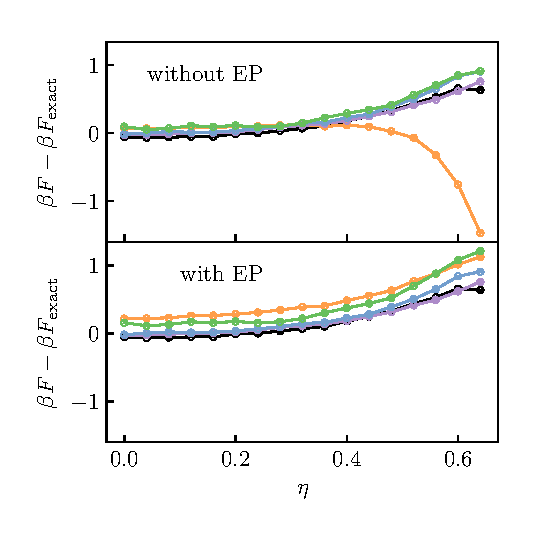
\includegraphics[width=0.9\linewidth,outer]{ep-n7}
  \caption[Errors in analytical integration techniques for the free energies of $n=7$ structures]{
    Errors in analytic integration techniques for free energies of the five $n = 7$ structures in Fig.\ \ref{fig:packings}.
    Top panel: simple integration ignoring hard sphere interactions not explicitly captured by the boundary conditions (section \ref{sec:no-ep-integration}).
    Bottom panel: expectation propagation (EP) integration which approximates the combined effect of boundary conditions and hard sphere interactions using (section \ref{sec:ep-integration}).
    In each case, the numerically exact result was obtained using thermodynamic integration described in chapter \ref{chapter:morphometric-applications}.
    The orange curve which deviates from the main trend without EP is the structure corresponding to a pentagonal bipyramid with broken five-fold symmetry; treatment of the broken bond with EP corrects the deviation.
  }
  \label{fig:ep-n7}
\end{SCfigure}

Matching moments between \eqref{eq:approximate-zeroth-moment} and \eqref{eq:exact-zeroth-moment} gives us
\begin{equation}
  \widetilde{Z}_i = \frac{\widehat{Z}_i}{Z_{\setminus i}}
  \sqrt{2 \pi (\sigma_{\setminus i}^2 + \widetilde{\sigma}_i^2)}
  \exp{\left(
    \frac{1}{2}
    \frac{(\mu_{\setminus i} - \widetilde{\mu}_i)^2}{\sigma_{\setminus i}^2 + \widetilde{\sigma}_i^2}
    \right)}.
\end{equation}
We calculate $\widehat{Z}_i / Z_{\setminus i}$ from \eqref{eq:exact-zeroth-moment} and then obtain the partition function from
\begin{equation}
  \begin{split}
    \log{\widetilde{Z}_i}
    =
    \frac{1}{2} \left(
    \log{(2\pi)} +
    \log{(\sigma_{\setminus i}^2 + \widetilde{\sigma}_i^2)} +
    \frac{(\mu_{\setminus i} - \widetilde{\mu}_i)^2}{\sigma_{\setminus i}^2 + \widetilde{\sigma}_i^2}
    \right.&
    \\
    \left.
    + \log{\left(\frac{\erf{\beta_i} - \erf{\alpha_i}}{2}\right)}
    \right)&
  \end{split}
\end{equation}
Giving the final partition function:
\begin{equation}
  \begin{split}
    \log{Z}
    =&
    \frac{1}{2} \left(
    (l-m) \log{2\pi}
    + \log\det{\vec{\Sigma}}
    + \vec{\nu} \cdot \vec{\Sigma} \cdot \vec{\nu}
    \right)
    \\ &
    + \sum_{i=1}^m \left(
    \log{\widetilde{Z}_i}
    - \frac{1}{2}
    \left(
    \log{\widetilde{\sigma}_i^2}
    + \widetilde{\nu}_i \widetilde{\mu}_i
    \right)
    \right)
  \end{split}
\end{equation}
where we have either
\begin{align}
  & \log{\widetilde{Z}_i}
  - \frac{1}{2}
  \left(
  \log{\widetilde{\sigma}_i^2}
  + \widetilde{\nu}_i \widetilde{\mu}_i
  \right)
  \nonumber \\ =&
  \frac{1}{2} \left(
  \log{(2\pi)} +
  \log{(\sigma_{\setminus i}^2 + \widetilde{\sigma}_i^2)} +
  \frac{(\mu_{\setminus i} - \widetilde{\mu}_i)^2}{\sigma_{\setminus i}^2 + \widetilde{\sigma}_i^2}
  \right.
  \nonumber \\ & \qquad
  \left.
  + \log{\left(\frac{\erf{\beta_i} - \erf{\alpha_i}}{2}\right)}
  - \log{\widetilde{\sigma}_i^2}
  - \widetilde{\nu}_i \widetilde{\mu}_i
  \right)
  \nonumber \\ =&
  \frac{1}{2} \left(
  \log{(2\pi)} +
  \log{\left(\frac{\sigma_{\setminus i}^2 + \widetilde{\sigma}_i^2}{\widetilde{\sigma}_i^2}\right)}
  + \frac{(\mu_{\setminus i} - \widetilde{\mu}_i)^2}{\sigma_{\setminus i}^2 + \widetilde{\sigma}_i^2}
  \right.
  \nonumber \\ & \qquad
  \left.
  - \widetilde{\nu}_i \widetilde{\mu}_i
  + \log{\left(\frac{\erf{\beta_i} - \erf{\alpha_i}}{2}\right)}
  \right)
  \nonumber \\ =&
  \frac{1}{2} \left(
  \log{(2\pi)} +
  \log{(1 + \widetilde{\tau}_i \sigma_{\setminus i}^2)}
  + \frac{\widetilde{\tau}_i \mu_{\setminus i}^2 - 2\widetilde{\nu}_i \mu_{\setminus i} - \widetilde{\nu}_i^2 \sigma_{\setminus i}^2}
  {1 + \widetilde{\tau}_i \sigma_{\setminus i}^2}
  \right.
  \nonumber \\ & \qquad
  \left.
  + \log{\left(\frac{\erf{\beta_i} - \erf{\alpha_i}}{2}\right)}
  \right)
\end{align}
or for small $\sigma_i^2 - \widetilde{\sigma}_i^2$ we use
\begin{equation}
  \begin{split}
    &
    \log{\widetilde{Z}_i}
    - \frac{1}{2}
    \left(
    \log{\widetilde{\sigma}_i^2}
    + \widetilde{\nu}_i \widetilde{\mu}_i
    \right)
    \\ =&
    \frac{1}{2} \left( -\log{\vec{c}_i \cdot \vec{\Sigma} \cdot \vec{c}_i} \right)
    + a_i \mu_i
    - \frac{a_i^2 \sigma_i^2}{2}
    - \frac{\widetilde{\nu}_i \widetilde{\mu}_i}{2}
    \\ & + 
    \log{\left(
      \int_0^{\delta_i}
      \exp{\left( -\frac{(x_i - (\mu_i + a_i \sigma_i^2))^2}{2 \vec{c}_i \cdot \vec{\Sigma} \cdot \vec{c}_i} +
        \frac{(x_i - \widetilde{\mu}_i)^2}{2 \widetilde{\sigma}_i^2} -a_i x_i \right)} \, dx_i
      \right)}.
  \end{split}
\end{equation}

\begin{SCfigure}
  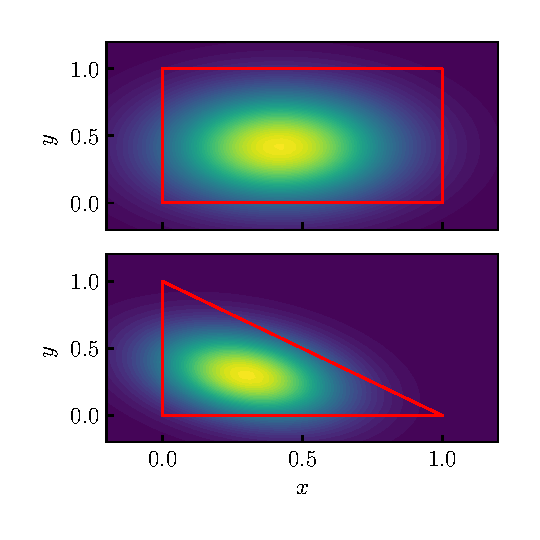
\includegraphics[width=0.9\linewidth,outer]{ep-pdf}
  \caption[Approximate probability distribution for integrating areas of simple 2d shapes]{
    Approximate (Gaussian) probability distribution $q(x,y)$ produced by expectation propagation for integrating over a square (top) and a right-angled triangle (bottom).
    In each panel the boundary of the true integration area is indicated by red lines.
  }
  \label{fig:ep-pdf}
\end{SCfigure}

\section{Worked example: area of a triangle}

As a simple worked example we consider the area of a right-angled triangle with vertices $(0,0)$, $(1,0)$, and $(0,1)$ i.e.\ half of the unit square.
We can write this area as the integral over a box
\begin{equation}\label{eq:ep-area-integral}
  A_\Delta = \int_0^1 \int_0^1 \Theta(1 - x - y) \, dx dy
  = \frac{1}{2}
\end{equation}
where $\Theta(\cdot)$ is the Heaviside function.
The exact result is fairly trivial, but it has the same form as the integrals we have been studying with e.g.\ $x,y$ representing the contact particles and $\Theta(1 - x - y)$ representing an additional hard sphere interaction between non-contact particles.
As such, we can evaluate the area using expectation propagation giving $A_\Delta^\mathrm{EP} \simeq 0.515$ for an error of about 3\%.
The effective probability distribution $p(x,y)$ for this integral is shown in \ref{fig:ep-pdf} (lower panel) which illustrates how the method builds in geometric information of additional constraints (in this case $\Theta(1 - x - y)$.
The distribution for the equivalent integral without this constraint is shown in the same figure (upper panel).
As an extension of the above problem we introduce an external field representing the perturbation expansion of the potential of mean force $\phi^{(n)}$.
We obtain the integral
\begin{equation}\label{eq:ep-triangle-integral}
  Z_\Delta = \int_0^1 \int_0^1 \Theta(1 - x - y) e^{-A_x x  A_y y} \, dx dy
\end{equation}
with the errors of expectation propagation shown in Fig.\ \ref{fig:ep-errors}.
The error of 3\% in the area is recovered in the limit $\vec{A} \to 0$, which increases to a maximum of around 4\% at moderate field strength.
At very large field strengths the error drops to essentially zero as the effect of the extra boundary condition is not seen, and the method becomes exact.

\begin{SCfigure}
  \includegraphics[width=0.9\linewidth,outer]{ep-errors}
  \caption[Errors in expectation propagation for integrating a field over a triangle]{
    Errors in expecation propagation for integrating a field over a triangle.
    The exact integral is given by \eqref{eq:ep-triangle-integral}, taking field $\vec{A} = (A, A)$.
  }
  \label{fig:ep-errors}
\end{SCfigure}

\section{Properties of multivariate Gaussians}
\label{sec:gaussian-properties}

\todo{Write opener}

The multivariate Gaussian is defined as
\begin{equation}
  \begin{split}
    \mathcal{N}(\vec{x}; \vec{\mu}, \vec{\Sigma})
    :=&
    \frac{1}{\sqrt{ (2\pi)^l \det{\vec{\Sigma}} }}
    \exp{\left(
      - \frac{1}{2} (\vec{x} - \vec{\mu}) \cdot \vec{\Sigma}^{-1} \cdot (\vec{x} - \vec{\mu})
      \right)}
    \\
    =&
    \frac{1}{\sqrt{ (2\pi)^l \det{\vec{\Sigma}} }}
    \exp{\left(
      - \frac{\vec{x} \cdot \vec{\Sigma}^{-1} \cdot \vec{x}}{2}
      + \vec{x} \cdot \vec{\Sigma}^{-1} \cdot \vec{\mu}
      - \frac{\vec{\mu} \cdot \vec{\Sigma}^{-1} \cdot \vec{\mu}}{2}
      \right)}
  \end{split}
\end{equation}
where $\vec{x} \in \mathbb{R}^l$ is the Gaussian distributed vector in our phase space, with mean $\vec{\mu} \in \mathbb{R}^l$ and (positive-definite) covariance matrix $\vec{\Sigma} \in \mathbb{R}^{l \times l}$.

In the EP algorithm we wrote the multivariate Gaussian approximation in $q$ as the product of univariate Gaussians from the tile distributions approximating the boundary conditions.
To show this, consider the product of univariate Gaussians:
\begin{align}
  %\begin{split}
    &
    \prod_{i=1}^m
    \mathcal{N}(\vec{c}_i \cdot \vec{x}; \widetilde{\mu}_i, \widetilde{\sigma}_i^2)
    %\nonumber \\ =&
    =
    \prod_{i=1}^m
    \left(
    \frac{1}{\sqrt{ 2\pi \widetilde{\sigma}_i^2 }}
    \exp{\left(
      - \frac{1}{2} \frac{(\vec{c}_i \cdot \vec{x} - \widetilde{\mu}_i)^2}{\widetilde{\sigma}_i^2}
      \right)}
    \right)
    %% \nonumber \\ =&
    %% \prod_{i=1}^m
    %% \left(
    %% \frac{1}{\sqrt{ 2\pi \widetilde{\sigma}_i^2 }}
    %% \exp{\left(
    %%   - \frac{(\vec{c}_i \cdot \vec{x})^2}{2\widetilde{\sigma}_i^2}
    %%   + \frac{\widetilde{\mu}_i(\vec{c}_i \cdot \vec{x})}{\widetilde{\sigma}_i^2}
    %%   - \frac{\widetilde{\mu}_i^2}{2\widetilde{\sigma}_i^2}
    %%   \right)}
    %% \right)
    \nonumber \\ =&
    \prod_{i=1}^m
    \left(
    \frac{1}{\sqrt{ 2\pi \widetilde{\sigma}_i^2 }}
    \exp{\left(-\frac{\widetilde{\mu}_i^2}{2\widetilde{\sigma}_i^2}\right)}
    \right)
    \exp{\left( \sum_{i=1}^m \left(
      - \frac{(\vec{c}_i \cdot \vec{x})^2}{2\widetilde{\sigma}_i^2}
      + \frac{\widetilde{\mu}_i(\vec{c}_i \cdot \vec{x})}{\widetilde{\sigma}_i^2}
      \right) \right)}
    %% \nonumber \\ =&
    %% \prod_{i=1}^m
    %% \left(
    %% \frac{1}{\sqrt{ 2\pi \widetilde{\sigma}_i^2 }}
    %% \exp{\left(-\frac{\widetilde{\nu}_i \widetilde{\mu}_i}{2}\right)}
    %% \right)
    %% \exp{\left( \sum_{i=1}^m \left(
    %%   - \vec{x} \cdot \frac{\vec{c}_i \otimes \vec{c}_i}{2\widetilde{\sigma}_i^2} \cdot \vec{x}
    %%   + (\widetilde{\nu}_i\vec{c}_i) \cdot \vec{x}
    %%   \right) \right)}
    %% \nonumber \\ =&
    %% \prod_{i=1}^m
    %% \left(
    %% \frac{1}{\sqrt{ 2\pi \widetilde{\sigma}_i^2 }}
    %% \exp{\left(-\frac{\widetilde{\nu}_i \widetilde{\mu}_i}{2}\right)}
    %% \right)
    %% \mathcal{N}(\vec{x}; \vec{\mu}, \Sigma)
    %% \;
    %% \sqrt{ (2\pi)^l \det{\vec{\Sigma}} }
    %% \;
    %% \exp{\left( \frac{\vec{\mu} \cdot \vec{\Sigma}^{-1} \cdot \vec{\mu}}{2} \right)}
    \nonumber \\ =&
    \prod_{i=1}^m
    \left(
    \frac{1}{\sqrt{ 2\pi \widetilde{\sigma}_i^2 }}
    \exp{\left(-\frac{\widetilde{\nu}_i \widetilde{\mu}_i}{2}\right)}
    \right)
    \mathcal{N}(\vec{x}; \vec{\mu}, \Sigma)
    \;
    \sqrt{ (2\pi)^l \det{\vec{\Sigma}} }
    \;
    \exp{\left( \frac{\vec{\nu} \cdot \vec{\Sigma} \cdot \vec{\nu}}{2} \right)}
    \nonumber \\ =&
    Z \mathcal{N}(\vec{x}; \vec{\mu}, \Sigma)
  %\end{split}
  \label{eq:combined-normals}
\end{align}
with
\begin{subequations}
\begin{align}
  \widetilde{\nu}_i &= \frac{\widetilde{\mu}_i}{\widetilde{\sigma}_i^2} \\
  \vec{\Sigma}^{-1} &= \sum_{i=1}^m \frac{\vec{c}_i \otimes \vec{c}_i}{\widetilde{\sigma}_i^2}
  \label{eq:combined-normals-sigma}
  \\
  \vec{\mu} &=
  \vec{\Sigma} \cdot \left( \sum_{i=1}^m \widetilde{\nu}_i \vec{c}_i \right)
  = \vec{\Sigma} \cdot \vec{\nu}
  \\
  \vec{\nu} &= \sum_{i=1}^m \widetilde{\nu}_i \vec{c}_i
  \label{eq:combined-normals-nu}
  \\
  Z &=
  \sqrt{ (2\pi)^{l-m} \det{\vec{\Sigma}} }
  \;
  \exp{\left( \frac{\vec{\nu} \cdot \vec{\Sigma} \cdot \vec{\nu}}{2} \right)}
  \prod_{i=1}^m
  %\left(
  \frac{1}{\sqrt{ \widetilde{\sigma}_i^2 }}
  \exp{\left(-\frac{\widetilde{\nu}_i \widetilde{\mu}_i}{2}\right)}
  %\right)
  \label{eq:combined-normals-Z}
\end{align}
\end{subequations}
From this we find that
\begin{equation}
  \log{Z} =
  \frac{l-m}{2} \log{2\pi} +
  \frac{1}{2} \log\det{\vec{\Sigma}} +
  \frac{\vec{\nu} \cdot \vec{\Sigma} \cdot \vec{\nu}}{2} -
  \sum_{i=1}^m
  \left(
  \frac{1}{2} \log{\widetilde{\sigma}_i^2} +
  \frac{\widetilde{\nu}_i \widetilde{\mu}_i}{2}
  \right)
\end{equation}
Finally, note that
\begin{equation}\label{eq:biased-normal}
  e^{-\vec{a} \cdot \vec{x}} \mathcal{N}(\vec{x}; \vec{\mu}, \vec{\Sigma})
  =
  \exp{\left( \frac{\vec{a} \cdot \vec{\Sigma} \cdot \vec{a}}{2} - \vec{a} \cdot \vec{\mu} \right)} \;
  \mathcal{N}(\vec{x}; \vec{\mu} - \vec{\Sigma}\cdot\vec{a}, \vec{\Sigma}).
\end{equation}

\todo{Write closer}

\ifdefined\includebibliography
  \newgeometry{margin=1in}
  \printbibliography
\fi

\end{document}

\end{appendices}

%\end{spacing}

\newgeometry{margin=1in}
\printbibliography[heading=bibintoc]

\end{document}
